% Options for packages loaded elsewhere
\PassOptionsToPackage{unicode}{hyperref}
\PassOptionsToPackage{hyphens}{url}
\PassOptionsToPackage{dvipsnames,svgnames,x11names}{xcolor}
%
\documentclass[
  12pt,
]{book}
\usepackage{amsmath,amssymb}
\usepackage{lmodern}
\usepackage{iftex}
\ifPDFTeX
  \usepackage[T1]{fontenc}
  \usepackage[utf8]{inputenc}
  \usepackage{textcomp} % provide euro and other symbols
\else % if luatex or xetex
  \usepackage{unicode-math}
  \defaultfontfeatures{Scale=MatchLowercase}
  \defaultfontfeatures[\rmfamily]{Ligatures=TeX,Scale=1}
\fi
% Use upquote if available, for straight quotes in verbatim environments
\IfFileExists{upquote.sty}{\usepackage{upquote}}{}
\IfFileExists{microtype.sty}{% use microtype if available
  \usepackage[]{microtype}
  \UseMicrotypeSet[protrusion]{basicmath} % disable protrusion for tt fonts
}{}
\makeatletter
\@ifundefined{KOMAClassName}{% if non-KOMA class
  \IfFileExists{parskip.sty}{%
    \usepackage{parskip}
  }{% else
    \setlength{\parindent}{0pt}
    \setlength{\parskip}{6pt plus 2pt minus 1pt}}
}{% if KOMA class
  \KOMAoptions{parskip=half}}
\makeatother
\usepackage{xcolor}
\usepackage[margin = 2cm]{geometry}
\usepackage{longtable,booktabs,array}
\usepackage{calc} % for calculating minipage widths
% Correct order of tables after \paragraph or \subparagraph
\usepackage{etoolbox}
\makeatletter
\patchcmd\longtable{\par}{\if@noskipsec\mbox{}\fi\par}{}{}
\makeatother
% Allow footnotes in longtable head/foot
\IfFileExists{footnotehyper.sty}{\usepackage{footnotehyper}}{\usepackage{footnote}}
\makesavenoteenv{longtable}
\usepackage{graphicx}
\makeatletter
\def\maxwidth{\ifdim\Gin@nat@width>\linewidth\linewidth\else\Gin@nat@width\fi}
\def\maxheight{\ifdim\Gin@nat@height>\textheight\textheight\else\Gin@nat@height\fi}
\makeatother
% Scale images if necessary, so that they will not overflow the page
% margins by default, and it is still possible to overwrite the defaults
% using explicit options in \includegraphics[width, height, ...]{}
\setkeys{Gin}{width=\maxwidth,height=\maxheight,keepaspectratio}
% Set default figure placement to htbp
\makeatletter
\def\fps@figure{htbp}
\makeatother
\setlength{\emergencystretch}{3em} % prevent overfull lines
\providecommand{\tightlist}{%
  \setlength{\itemsep}{0pt}\setlength{\parskip}{0pt}}
\setcounter{secnumdepth}{5}
\ifLuaTeX
\usepackage[bidi=basic]{babel}
\else
\usepackage[bidi=default]{babel}
\fi
\babelprovide[main,import]{spanish}
% get rid of language-specific shorthands (see #6817):
\let\LanguageShortHands\languageshorthands
\def\languageshorthands#1{}
\usepackage{setspace}
%\linespread{1.5}
%\usepackage{tikz}
%\usetikzlibrary{shapes,arrows}
\usepackage{pdflscape}
\newcommand{\blandscape}{\begin{landscape}}
\newcommand{\elandscape}{\end{landscape}}
\renewcommand{\thesection}{\Roman{section}}
\renewcommand{\thesubsection}{\Alph{subsection}}
\usepackage{booktabs}
\usepackage{amsthm}
\makeatletter
\def\thm@space@setup{%
  \thm@preskip=8pt plus 2pt minus 4pt
  \thm@postskip=\thm@preskip
}
\makeatother
\usepackage[spanish, spanishkw, onelanguage, linesnumbered, amsmath]{}
\ifLuaTeX
  \usepackage{selnolig}  % disable illegal ligatures
\fi
\usepackage[]{natbib}
\bibliographystyle{apalike}
\IfFileExists{bookmark.sty}{\usepackage{bookmark}}{\usepackage{hyperref}}
\IfFileExists{xurl.sty}{\usepackage{xurl}}{} % add URL line breaks if available
\urlstyle{same} % disable monospaced font for URLs
\hypersetup{
  pdftitle={Diseño y análisis estadístico en las encuestas de hogares de América Latina},
  pdfauthor={Andrés Gutiérrez},
  pdflang={es},
  colorlinks=true,
  linkcolor={blue},
  filecolor={Maroon},
  citecolor={Blue},
  urlcolor={Blue},
  pdfcreator={LaTeX via pandoc}}

\title{Diseño y análisis estadístico en las encuestas de hogares de América Latina}
\author{Andrés Gutiérrez\footnote{Experto Regional en Estadísticas Sociales - Comisión Económica para América Latina y el Caribe (CEPAL) - \href{mailto:andres.gutierrez@cepal.org}{\nolinkurl{andres.gutierrez@cepal.org}}}}
\date{2022-10-13}

\begin{document}
\maketitle

{
\hypersetup{linkcolor=}
\setcounter{tocdepth}{1}
\tableofcontents
}
\listoffigures
\listoftables
\hypertarget{prefacio}{%
\chapter*{Prefacio}\label{prefacio}}
\addcontentsline{toc}{chapter}{Prefacio}

\begin{figure}

\includegraphics[width=100px]{Pics/CClicence} \caption{Licencia de Creative Commons}\label{fig:unnamed-chunk-1}
\end{figure}

La versión online de este libro está licenciada bajo una \href{http://creativecommons.org/licenses/by-nc-sa/4.0/}{Licencia Internacional de Creative Commons para compartir con atribución no comercial 4.0}.

La coordinación sustantiva de la colección Metodologías de la CEPAL está a cargo de Rolando Ocampo, Director de la División de Estadísticas de la Comisión Económica para América Latina y el Caribe (CEPAL).

Esta publicación es el resultado de un proceso de varios años de investigación e interacción con los países miembros en diversas asistencias técnicas concernientes con el diseño, rediseño y análisis posterior de las encuestas de hogares. Dicho proceso fue llevado a cabo por la División de Estadísticas de la CEPAL, bajo la coordinación de Rolando Ocampo, Director de la División de Estadísticas y de Xavier Mancero, Jefe de la Unidad de Estadísticas Sociales.

La redacción del documento estuvo a cargo de Andrés Gutiérrez, Asesor Regional en Estadísticas Sociales de la CEPAL. Las metodologías presentadas en este documento se han beneficiado de los valiosos aportes y sugerencias de funcionarios de la CEPAL, así como del personal de las Oficinas Nacionales de Estadística de los países beneficiarios de las asistencias técnicas durante los años entre 2017 y 2022. El autor agradece a Simone Ceccini, y a Hanwen Zhang por la lectura detallada de este documento y sus comentarios.

\hypertarget{resumen}{%
\chapter*{Resumen}\label{resumen}}
\addcontentsline{toc}{chapter}{Resumen}

Las encuestas de hogares son un instrumento necesario para realizar seguimiento a un conjunto amplio de indicadores requeridos para el diseño y evaluación de las políticas públicas. Las encuestas de hogares que se implementan en América Latina son de tipo y características diversas. Aunque los conceptos y procesos para su diseño y análisis guardan similitudes, este documento se enfoca principalmente en los procesos referidos a las encuestas de empleo y de propósitos múltiples, con las que los países estiman los principales indicadores relacionados con el mercado laboral, el nivel y distribución de ingresos y la condición de pobreza y las principales características sociodemográficas de la población. Se realiza un recorrido por los diferentes diseños de muestreo, las metodologías más usadas en la selección de las muestras y las estrategias de estimación de los parámetros de interés. También se revisan las técnicas utilizadas para medir el error de muestreo y los métodos disponibles para encarar desafíos como la ausencia de respuesta y la desactualización de los marcos de muestreo.

\textbf{UNBIS Keywords}. Encuestas por muestreo, encuestas de hogares, indicadores socioeconómicos.

\hypertarget{introducciuxf3n}{%
\chapter{Introducción}\label{introducciuxf3n}}

Este documento pretende revisar algunas de las metodologías más usadas por las ONE de América Latina en cuanto al diseño y análisis estadístico de las encuestas de hogares y puede servir de guía técnica a los estadísticos de la región que se encuentran involucrados en los procesos técnicos de este tipo de encuestas. De la misma forma, este documento considera conjuntamente los dos principales momentos de las encuestas: el diseño y el análisis. Nótese que estos momentos están escindidos por el levantamiento de la información en campo y parten la realización de la encuesta en dos. Los lectores que están familiarizados con la investigación social a través de las encuestas de hogares encontrarán que estas operaciones estadísticas se planean teniendo en cuenta muchos pormenores que podrían suceder en campo. Es por esto que el trabajo de los investigadores en las ONE es que el mismo diseño que se planificó se logre plasmar en la información recolectada en la de base de microdatos de las encuestas. En este segundo momento es cuando se debe asegurar que lo que se planificó efectivamente sea incorporado en el análisis de esta información.

Desde esta perspectiva, este documento se aborda en tres partes sustantivas que definen la planeación y el análisis de la mayoría de las encuestas de hogares en América Latina y el Caribe. La primera parte, contenida en los capítulos del uno al ocho, se refiere a la planeación de una encuesta y a la definición del diseño estadístico, que comprende - entre otras cosas - la generación de una medida de probabilidad discreta que soportará la inferencia basada en el principio de representatividad. En esta parte se aborda con más detalle los elementos básicos que se consideran por lo regular en los diseños de las encuestas de hogares. Un aspecto relevante es que, si bien este documento considera que las encuestas de hogares tienen muchos elementos en común, diferencia de forma cuidadosa las particularidades de cada tipo de encuesta. Por ejemplo, se trata el tema del diseño de las encuestas rotativas y se profundiza en los diferentes parámetros que se pueden considerar en este tipo de operaciones; asimismo, describe las características metodológicas que se deben considerar al momento de diseñar la encuesta y revisa los conceptos esenciales que determinarán el tipo de aplicación que se debe considerar. Asimismo, se describen los principales diseños de muestreo que se utilizan en este tipo de estudios y se expone de forma estándar los conceptos de estratificación y aglomeración de las poblaciones. Estos conceptos se complementan con varias aplicaciones prácticas para determinar el tamaño de muestra adecuado para lograr los objetivos de una investigación planeada con base en las encuestas de hogares. A pesar de que la literatura relacionada con la práctica del muestreo es relativamente abundante, existen pocos ejemplos prácticos que logren representar la problemática del tamaño de muestra y el lector podrá encontrar herramientas ilustrativas basadas en múltiples escenarios de la problemática social.

La segunda parte, contenida en los capítulos del nueve al quince, aborda los principios metodológicos para el correcto procesamiento de las encuestas transversales, analizadas para representar un momento específico en el tiempo. Se revisan con detenimiento los procesos ponderación en la encuesta y generación de los factores de expansión que se aplicarán a la información contenida en la base de datos para que se poder generar exitósamente inferencias a nivel nacional o regional. Si hay algo que distingue el análisis de las encuestas de cualquier otro tipo de estudio estadístico es que las propiedades importantes como insesgamiento, consistencia y eficiencia están basadas en el diseño de muestreo y no en supuestos metodológicos ligados a algún modelo estocástico. Además de analizar las principales metodologías de estimación, se presta especial atención a la estimación del error de muestreo, que no es otra cosa que una función de la varianza de las estimaciones, y se presentan las metodologías más comunes en términos de aproximaciones teóricas y computacionales al error de muestreo. Los procesos de imputación y ausencia de respuesta también son abordados, con el objetivo de recuperar tanta información como sea posible para que el investigador pueda contar con una base de datos rectangular y completa. En aquellos casos en donde la imputación no resulta ser una técnica adecuada para completar la información faltante, es necesario realizar ajustes sistemáticos en los factores de expansión para que la muestra efectiva siga siendo una muestra representativa de toda la población. El último capítulo de esta parte muestra algunos enfoques útiles en la detección de datos atípicos, y la mitigación del impacto del error no muestral en las respuestas obtenidas.

La tercera y última parte, contenida en los capítulos 16 al 20, avanza hacia los principios del procesamiento avanzado en un sistema integrado de encuestas de hogares que permite la agregación y/o combinación de diferentes oleadas de las encuestas, y así permitir la inferencia en un lapso más amplio. De esta forma, se presentan detalladamente los procesos que se surten cuando se agregan encuestas a lo largo del tiempo. Para aquellas encuestas que se definen a partir de estructuras rotativas, se presenta un enfoque metodológico que permite crear bases de datos longitudinales (tipo panel) para la estimación de flujos brutos, entre otros. Acudiendo a la perspectiva de CEPAL, también se presentan los criterios de calidad que se deberían tener en cuenta para decidir si una cifra, resultante de un proceso de estimación estadística basada en encuestas de hogares, debería ser o no publicada a la sociedad.

Por último, en los anexos del documento se presenta una discusión acerca del uso presente de las encuestas de hogares y los retos que depara el futuro en materia de la medición de indicadores sociales a través de las encuestas de hogares. Asimismo, se contempla una revisión del software que se utiliza actualmente en los ONE para llevar a cabo esta ardua tarea de diseñar y analizar las encuestas de hogares, una revisión rápida de algunas de las encuestas de la región, así como algunas directrices que se deberían considerar al momento de documentar los procesos asociados a las encuestas de hogares.

En este documento, los profesionales y metodólogos de las Oficinas Nacionales de Estadística de la región latinoamericana podrán encontrar una guía práctica sobre todas las cuestiones técnicas relacionadas con el devenir de una encuesta de hogares: desde la planeación, pasando por el análisis básico y adentrándose en los análisis complejos propios de una recolección continua. Este libro se escribe con el interés de recopilar las mejores herramientas técnicas y actualizar los métodos usados por las ONE en el diseño y rediseño de las encuestas de hogares. En la literatura, también existen esfuerzos realizados por la Organización de las Naciones Unidas para llevar la teoría básica de las encuestas de hogares al español, como por ejemplo \citet{UnitedNations_2005} y \citet{UnitedNations_2008}. Sin embargo, este documento complementa estos valiosos recursos ahondando de una manera más profunda en los temas estadísticos relevantes para una mejor implementación de los procesos técnicos relacionados con las encuestas de hogares. Por tanto, aunque no es una condición necesaria, se recomienda que el lector de este documento tenga una amplia experiencia en el diseño y análisis de encuestas de hogares para su mejor aprovechamiento.

\hypertarget{quuxe9-es-una-encuesta}{%
\section{¿Qué es una encuesta?}\label{quuxe9-es-una-encuesta}}

\citet{Groves_Fowler_Couper_Lepkowski_Singer_Tourangeau_2009} afirma que una encuesta es un método sistemático para obtener información de (una muestra de) entes, con el fin de construir descriptores cuantitativos de los atributos de una población más grande, de la cual los entes son miembros.
Por otro lado, Wikipedia afirma que una encuesta es un estudio observacional en el cual el investigador busca recaudar datos por medio de un cuestionario pre-diseñado, y no modificar el entorno ni controlar el proceso que está en observación (como sí lo hace en un experimento).

Además, los datos se obtienen a partir de realizar un conjunto de preguntas normalizadas dirigidas a una muestra representativa o al conjunto total de la población estadística en estudio, formada a menudo por personas, empresas o entes institucionales, con el fin de conocer estados de opinión, características o hechos específicos. Hay una diferencia sustancial entre los sondeos y las encuestas; de esta forma,

\begin{itemize}
\tightlist
\item
  \textbf{Sondeo}: es la traducción de \emph{poll}, que a su vez viene del antiguo alemán referente a cabeza y se utilizaba para contar: ``contar cabezas''.
\item
  \textbf{Encuesta}: es la traducción de \emph{survey}, que a su vez viene del latín \emph{super} (sobre) y \emph{videre} (observar).
\end{itemize}

En general, la primera expresión aparece muchas más veces en el sector privado, en estudios de opinión y de consumo. Un sondeo no será jamás utilizado para obtener estadísticas oficiales en estudios gubernamentales o en dominios científicos. Sin embargo, los sondeos muchas veces opacan la perspectiva científica de las cifras y pueden llevar a conclusiones inexactas acerca de la realidad de una problemática. No todos los procesos de recolección de información se pueden llamar encuestas; para efectos de este documento seguiremos la definición de \citet{Groves_Fowler_Couper_Lepkowski_Singer_Tourangeau_2009}, quienes afirman que una tendrá las siguientes características:

\begin{enumerate}
\def\labelenumi{\arabic{enumi}.}
\tightlist
\item
  Los datos son recopilados mediante preguntas a personas.
\item
  Las respuestas son compiladas cuando: a) un encuestador pregunta y registra las respuestas del entrevistado o b) el encuestado lee y registra sus propias respuestas.
\item
  Los datos son recolectados de un subgrupo de personas pertenecientes a la población de interés.
\end{enumerate}

Nótese que el último ítem de la anterior marca una clara diferenciación con los censos de población y vivienda. Las encuestas de hogares son un caso particular de investigación social que indaga acerca de características específicas a nivel del individuo, del hogar o de la vivienda, con el fin de obtener inferencias precisas acerca de constructos de interés. Por su naturaleza, estas investigaciones están relacionadas con variables de salud, educación, ingresos, gastos, situación laboral, acceso y uso de servicios, entre muchas otras. En algunas ocasiones, las encuestas de hogares tienen como objetivo la estimación de uno o varios indicadores que resumen un constructo económico o social. Por ejemplo, la tasa de pobreza, la tasa de desocupación, el gasto promedio en alimentación, entre muchos otros. Sin embargo, existe una tendencia creciente de extender las encuestas a constructos más diversos. Es así como cada vez tienen más espacio las encuestas que incluyen diversos módulos en sus cuestionarios, conocidas como encuestas de propósitos múltiples, como una fuente relevante de información que permite monitorear indicadores sociales.

En estas encuestas, el hogar es la unidad de análisis, la cual ha sido definida por la División de Estadística de la Organización de las Naciones Unidas \citep{United-Nations_2011} como:

\begin{quote}
\begin{enumerate}
\def\labelenumi{\alph{enumi}.}
\tightlist
\item
  Un grupo de dos o más personas que se combinan para ocupar la totalidad o parte de una vivienda y para proporcionarse alimentos y posiblemente otros artículos esenciales para la vida. El grupo puede estar compuesto solo de personas relacionadas o de personas no relacionadas o de una combinación de ambos. El grupo también puede compartir sus ingresos.
\item
  Una persona que vive sola en una vivienda separada o que ocupa, como huésped, una habitación (o habitaciones) separada de una vivienda pero que no se une a ninguno de los otros ocupantes de la vivienda para formar parte de una hogar de múltiples personas.
\end{enumerate}
\end{quote}

Nótese que la anterior definición refleja una dinámica en los hogares, los cuales constantemente se crean, desaparecen o se unen, por lo cual es necesario aproximarse desde distintos enfoques para abordar el problema de la medición de indicadores sociales. En América Latina, existen una gran variedad de encuestas que abordan diferentes problemáticas sociales. Todas y cada una de ellas han sido diseñadas cuidadosamente para que respondan a las necesidades de la sociedad. Este documento plantea una recopilación de las técnicas usadas tanto en su diseño, como en su análisis.

No todas las encuestas se diseñan de la misma forma y por ende debe haber una distinción entre ellas. Por ejemplo, \citet{Kalton_Citro_1993} afirman que las encuestas de hogares pueden clasificarse en varios tipos:

\begin{itemize}
\tightlist
\item
  \emph{Encuestas repetidas}, definidas como una serie de encuestas transversales aplicadas en diferentes momentos del tiempo con el mismo diseño metodológico, en donde la selección de hogares se hace de forma independiente para cada aplicación.
\item
  \emph{Encuestas tipo panel}, para las cuales los datos son recolectados en diferentes momentos del tiempo utilizando la misma muestra de hogares en el tiempo.
\item
  \emph{Encuestas rotativas}, en donde un porcentaje de hogares se mantiene en un periodo de tiempo respondiendo la encuesta y en cada aplicación algunos hogares son reemplazados por nuevos hogares de forma planificada.
\end{itemize}

El diseño de la encuesta dependerá sistemáticamente del objetivo de la medición. Por ejemplo, \citet{Kalton_2009} afirma que es prudente hacer un buena inversión en el desarrollo e implementación de un buen diseño para amortizar los costos de todo el estudio. Por lo tanto, lo que se quiere al diseñar una encuesta de hogares es que sea un instrumento confiable, que brinde estimaciones exactas y precisas, puesto que de lo contrario no se podrían monitorear las políticas públicas y los indicadores de interés de forma consistente. Por ejemplo, uno de los indicadores sociales de mayor uso es la tasa de desocupación, que mide la razón entre la cantidad de personas que se encuentran desocupados, pero que forman parte del mercado de trabajo. Las encuestas de empleo tienen características particulares, diferentes a las de las encuestas que miden otro tipo de constructos. \citet{Duncan_Kalton_1987} mencionan que las encuestas de hogares pueden proveer estimaciones de los parámetros poblacionales en distintos puntos del tiempo, por ejemplo, la estimación de la tasa de desocupación mensual; proveer estimaciones del cambio neto de los parámetros poblacionales entre periodos de tiempo, por ejemplo, el cambio en la tasa de desocupación entre dos periodos consecutivos; o incluso medir varios componentes de cambio individual, por ejemplo cambios brutos en la situación laboral de los jefes de hogar, para lo cual se requiere que la encuesta contemple un diseño de panel o de panel rotativo.

La medición de los indicadores en el mercado de trabajo es sólo un pequeño componente en el vasto y amplio universo de posibilidades de medición que brindan las encuestas de hogares. Por esta razón, este tipo de levantamientos se ha convertido en una herramienta fundamental para medir indicadores sociales en todo el mundo y que, en particular, permiten que los países de América Latina puedan hacer seguimiento a su desarrollo económico y social. A continuación se introducen algunas temáticas de interés para las cuales, su seguimiento depende en gran manera de la realización de encuestas de hogares.

\hypertarget{objetivos-de-desarrollo-sostenible-y-otros-indicadores-regionales}{%
\section{Objetivos de Desarrollo Sostenible y otros indicadores regionales}\label{objetivos-de-desarrollo-sostenible-y-otros-indicadores-regionales}}

Las encuestas de hogares pueden ser utilizado como herramienta para monitorear el progreso de los países en términos de metas y objetivos comunes. Es así como en 2015, la Asamblea General de la Organización de las Naciones Unidas aprobó una resolución que plantea un plan de acción en favor de las personas, el planeta y la prosperidad \citep{United_Nations_2015}. Esa resolución propone el seguimiento de 17 Objetivos de Desarrollo Sostenible (\href{https://sustainabledevelopment.un.org}{ODS}) y 169 metas de carácter integrado e indivisible que se conjugan en las dimensiones económica, social y ambiental. Para realizar el seguimiento a los ODS es posible utilizar diferentes fuentes de información, como censos, registros administrativos, registros estadísticos, proyecciones demográficas y también las encuestas de hogares \citep{United_Nations_2016}. En particular, cada una de las metas de los ODS contiene indicadores, muchos de los cuales no pudieran ser estimados de no ser por la información disponible en las encuestas de hogares.

Por ejemplo, el primer objetivo busca \emph{poner fin a la pobreza en todas sus formas en todo el mundo}. La primera meta de este objetivo establece la \emph{erradicación de la pobreza extrema para todas las personas en el mundo}. Asimismo, la segunda meta de este objetivo motiva a los países a \emph{reducir al menos a la mitad la proporción de hombres, mujeres y niños y niñas de todas las edades que viven en la pobreza en todas sus dimensiones con arreglo a las definiciones nacionales}. Para realizar una medición sistemática de la pobreza monetaria las encuestas de hogares son un insumo fundamental. En una primera instancia se deben definir a nivel nacional los umbrales monetarios (líneas de pobreza) sobre los cuales se clasifican a los hogares como pobres extremos, pobres relativos o no pobres. Estos umbrales vienen supeditados directamente a la realización de las encuestas de ingresos y gastos, las cuales se realizan cada cinco o diez años en los países de la región (CEPAL 2018). De forma sistemática, la medición de la pobreza monetaria se realiza con encuestas continuas que contienen módulos específicos de ingreso, los cuales indagan por todas las fuentes de ingreso, tanto de las personas como del hogar. Con base en las líneas de pobreza definidas anteriormente, se clasifica a las personas en alguna de las categorías de la pobreza.

De la misma manera, el objetivo \textbf{8} busca \emph{promover el crecimiento económico sostenido, inclusivo y sostenible, el empleo pleno y productivo y el trabajo decente para todos}. Claramente de este objetivo se desprenden indicadores que permiten conocer la evolución de los países en la consecución de las metas. Dentro de este objetivo, se encuentra la meta \textbf{8.6} que apunta a reducir sustancialmente la proporción de jóvenes sin empleo y sin educación o entrenamiento. Esta meta se mide con el indicador \textbf{8.6.1} definido como la proporción de jóvenes (entre 15 y 24 años de edad) sin educación y sin empleo.

Son muchísimos más los ejemplos que se pueden enumerar en los cuales las encuestas de hogares juegan un rol fundamental para la medición de los indicadores y metas de los ODS definidos en la Agenda 2030; en este sentido la División de Estadísticas de las Naciones Unidas ha establecido en un análisis preliminar que un total de 77 de los indicadores de los Objetivos de Desarrollo Sostenible pueden obtenerse a partir de encuestas de hogares, cubriendo 13 de los 17 Objetivos; aunque con mayor concentración en las áreas de salud, educación, igualdad de género, pobreza, hambre, trabajo y justicia.

\hypertarget{estaduxedsticas-del-mercado-de-trabajo}{%
\subsection{Estadísticas del mercado de trabajo}\label{estaduxedsticas-del-mercado-de-trabajo}}

Desde otra perspectiva, en el marco de la Decimotercera Conferencia Internacional de Estadísticos del trabajo en 1982, la Organización Internacional del Trabajo (OIT) adoptó algunas directrices concernientes con la medición y análisis de estadísticas oficiales de la fuerza de trabajo, del empleo y del desempleo con miras a mejorar la comparabilidad de las cifras y mejorar su utilidad en los países \citep{OIT_1982}. En esta resolución se hace un énfasis especial en que las encuestas de hogares constituyen un medio apropiado de recopilación de datos sobre la población económicamente activa y que la planeación de estas investigaciones en los países debería ceñirse a las normas internacionales. Por consiguiente, la resolución afirma que las encuestas de hogares deberían:

\begin{enumerate}
\def\labelenumi{\arabic{enumi}.}
\tightlist
\item
  Brindar datos de la población económicamente activa, definida por las personas en edad laboral que se han integrado al mercado de trabajo (trabajadores o personas en búsqueda de empleo).
\item
  Proveer estadísticas básicas de sus actividades durante el año, así como las relaciones entre el empleo, ingreso y otras características económicas y sociales.
\item
  Proveer datos sobre otros temas particulares para responder a las necesidades a largo plazo y de índole permanente.
\end{enumerate}

En el año 2013, la OIT decidió revisar esta resolución y propuso algunos cambios en el marco de la decimonovena Conferencia Internacional de Estadísticos del Trabajo en donde se acogieron algunas modificaciones en términos de los objetivos de medición y el alcance de los sistemas nacionales de estadísticas del trabajo, el concepto de trabajo en todas sus formas, el empleo, la medición de las personas en situación de subutilización de la fuerza de trabajo, métodos de recopilación de datos, entre otras \citep{OIT_2013}. Las Oficinas Nacionales de Estadística (ONE) de América Latina actualizan los instrumentos de medición de las encuestas de hogares para que puedan responder a los nuevos retos en términos de la estimación de los parámetros de interés del trabajo remunerado o no remunerado para mantener la comparabilidad de las estadísticas laborales entre los países, proporcionando nuevos y mejores indicadores para contribuir al análisis de la dinámica del mercado laboral para poder brindar la información que la sociedad necesita a medida que evoluciona este constructo social.

\hypertarget{ingresos-y-gastos}{%
\subsection{Ingresos y gastos}\label{ingresos-y-gastos}}

Es importante resaltar que los indicadores de bienestar (en términos de ingresos y gastos) también hacen parte del conjunto de parámetros que se pueden estimar desde las encuestas de hogares. Medir el ingreso a partir de las encuestas de hogares se constituye en un reto metodológico para los institutos nacionales de estadística en el mundo, y particularmente en América Latina. Es recomendable seguir las directrices de la Comisión Económica para Europa que revisten una actualización de los estándares internacionales, recomendaciones y buenas prácticas en la medición del ingreso en los hogares. Por ejemplo, el llamado Grupo de Canberra ha revisado exhaustivamente el tópico de la estimación del ingreso estudiando las prácticas de algunos países en términos del aseguramiento de la calidad y la publicación de este tipo de estadísticas oficiales y ha provisto la siguiente definición de ingreso en el hogar \citep{United-Nations_2011}:

\begin{quote}
\emph{El ingreso del hogar se compone de las entradas monetarias, en especie o en servicios que por lo general son frecuentes y regulares, están destinadas al hogar o a los miembros del hogar por separado y se reciben a intervalos anuales o con mayor frecuencia. Durante el período de referencia en el que se reciben, tales entradas están potencialmente disponibles para el consumo efectivo y, habitualmente, no reducen el patrimonio neto del hogar.}
\end{quote}

Con base en lo anterior, el uso de las encuestas de hogares para estimar el ingreso reviste retos metodológicos mayores puesto que los entrevistados deben responder con precisión cuando se les indague por este constructo que contiene los ingresos personales de cada individuo en el hogar, como sueldos y salarios, ganancias, ingresos del empleo, pensiones, etc. y también los ingresos del hogar, incluidas las rentas por alquiler y los ingresos generados por el comercio. Por lo tanto, el diseño de la encuesta debe tener en cuenta la definición de un instrumento que sea relevante para el respondiente y le permita identificar y, en algunas ocasiones, recordar la información con un cierto grado de exactitud.

Por ejemplo, si el respondiente es empleado regular, el instrumento de medición debería planearse de tal manera que el entrevistado pueda recordar la información de interés, como los rubros de seguridad social hechos por su empleador. Por otro lado, si se requiere que el respondiente brinde información acerca de un determinado periodo de tiempo, el planteamiento de la pregunta, la forma de indagar y el entrenamiento de los encuestadores pueden sesgar sistemáticamente la respuesta y por consiguiente inducir estimaciones poco confiables. Mucho se ha investigado al respecto de cómo realizar preguntas certeras en este tipo de levantamientos y el lector interesado puede consultar los trabajos de \citet{Biemer_Lyberg_2003}, \citet{Presser_Rothgeb_Couper_Lessler_Martin_Martin_Singer_2004}, y \citet{Groves_Fowler_Couper_Lepkowski_Singer_Tourangeau_2009}.

\hypertarget{algunos-desafios-de-las-regiuxf3n-en-cuanto-a-la-producciuxf3n-de-las-encuestas-de-hogares}{%
\section{Algunos desafios de las región en cuanto a la producción de las encuestas de hogares}\label{algunos-desafios-de-las-regiuxf3n-en-cuanto-a-la-producciuxf3n-de-las-encuestas-de-hogares}}

La forma de medición de los indicadores sociales debe estar alineada con el diseño de la encuesta. Los equipos técnicos de los países deben ajustar sus metodologías a los requerimientos de la encuesta para proveer estadísticas oficiales que sean no sólo confiables y precisas sino eficientes en términos de los recursos que se destinan a la recolección de la información primaria, máxime cuando estos muchas veces se deben recortar por limitaciones en el presupuesto de los países.

En Latinoamérica se observa un incremento progresivo de la tasa de ausencia de respuesta debido al aumento de viviendas no entrevistadas que se origina en la expansión urbana y en la desactualización de los marcos de muestreo. La continua expansión urbana en la región hace que los encuestadores afronten retos mayores cuando llegan a un área de muestreo y no encuentran la vivienda que se supone que deberían entrevistar, o en vez de una vivienda ahora encuentran un edificio de apartamentos. Con el uso, cada vez más frecuente de los dispositivos de almacenamiento electrónico, es posible realizar un análisis mejor estructurado de los instrumentos de recolección de información. Por ejemplo, es posible programar saltos más complejos, estimar el tiempo promedio de respuesta en las preguntas del cuestionario, el tiempo promedio de respuesta en los bloques de preguntas, entre otras.

En el seguimiento a las metas de la Agenda 2030 y en la búsqueda del cumplimiento de los ODS, las Naciones Unidas ha expresado la necesidad de contar con estadísticas oficiales, no sólo a nivel nacional, sino a nivel de desagregaciones geográficas o de categorías demográficas de interés \citep{United_Nations_2017}. Es así como se plantea la siguiente necesidad a los países:

\begin{quote}
\emph{La disponibilidad de datos desagregados, oportunos y de alta calidad es vital para la toma de decisiones basada en la evidencia y para garantizar la responsabilidad de la implementación de la Agenda 2030. El seguimiento del progreso en los Objetivos de Desarrollo Sostenible requiere una cantidad sin precedentes de datos y estadísticas en todos los niveles, lo que plantea un desafío importante para los sistemas estadísticos nacionales e internacionales. La comunidad estadística mundial está trabajando para modernizar y fortalecer los sistemas estadísticos para abordar todos los aspectos de la producción y el uso de datos para el desarrollo sostenible.}
\end{quote}

Por supuesto, la región no es ajena a este reto y debe desde ya plantearse la necesidad de crear capacidad en los equipos técnicos de los INE que deberán utilizar como insumo las encuestas de hogares, los censos de población y los registros administrativos para poder establecer metodologías de estimación en las desagregaciones de interés, que como mínimo deberán clasificarse por sexo, grupos etarios, ingreso, raza, etnia, estado migratorio, discapacidad y localización geográfica \citep{United_Nations_2016}

Al respecto, uno de los primeros acercamientos al diseño de las encuestas de hogares para la publicación de estadísticas oficiales en dominios pequeños fue presentado por \citet{Sinngh_Gambino_Mantel_1994} en donde se plantean algunas consideraciones para la estimación de indicadores sociales a nivel de dominios pequeños. Sin embargo, más allá de considerar el diseño metodológico, ahora es posible considerar otro tipo de acercamientos inferenciales que pretenden estimar indicadores a nivel de estos dominios pequeños. \citet{Rao_Molina_2014} proveen un resumen exhaustivo de las técnicas más usadas en la diseminación de estadísticas oficiales en desagregaciones pequeñas. En América Latina, este tipo de metodologías, que utilizan como insumo principal a las encuestas de hogares, se aplican con mayor frecuencia. Por ejemplo, \citet{arias2007geography} realizan una estimación de la pobreza monetaria en las municipalidades de Bolivia utilizando los datos del censo poblacional del 2001; \citet{araujo20071990} resume la experiencia ecuatoriana de la estimación de la pobreza en los municipios, cantones y provincias; \citet{lopez2007poverty} presentan la estimación de indicadores de desarrollo humano utilizando estimación de áreas pequeñas en las municipalidades de México a través de la \emph{Encuesta Nacional de Ingresos y Gastos de los Hogares}. Finalmente, \citet{Casas_Cordero_Valencia_Encina_Lahiri_2016} presentan un ejercicio de estimación de la pobreza en Chile utilizando la encuesta \emph{Encuesta de Caracterización Socioeconómica Nacional}.

\hypertarget{el-paradigma-del-error-total}{%
\chapter{El paradigma del error total}\label{el-paradigma-del-error-total}}

Este capítulo describe muy someramente el paradigma de los errores que se cometen en una encuesta y cómo al tenerlos en cuenta en la etapa de planificación, es posible medirlos acertádamente y acotarlos con base en el principio de representatividad. En general, todos los procesos en una encuesta deben estar planificados de antemano, antes y después de la recolección de los datos. Por ejemplo, el cuestionario (instrumento de medición) debe estar muy bien diseñado para que las respuestas de las personas describan acertadamente las características de los entrevistados. De la misma forma, el subconjunto de personas que participan en la encuesta debe ser expandido con precisión y confiabilidad para que represente con certeza a la población de interés.

\citet{Beland_Dale_Dufour_Hamel_2005} describen los principales elementos del diseño de una encuesta de hogares y esta es una tarea que deben afrontar los equipos técnicos de las ONE en términos de aprender de las experiencias del pasado para mejorar los procesos operativos, metodológicos y logísticos en las siguientes aplicaciones de las encuestas. Es así como ante la nueva oleada de censos que se avecina en la próxima década, será natural actualizar los marcos de muestreo y con ello se viene un reto para los equipos técnicos encargados de la encuestas de hogares en América Latina que consiste en evaluar el impacto del cambio de los marcos de muestreo y sus efectos en la comparabilidad de las cifras oficiales.

En una encuesta, el interés no se centra en las características particulares de un individuo sino en las características de la población a la cual ese individuo pertenece. De esta forma, la inferencia siempre se realiza teniendo en mente agregados (indicadores) poblacionales. La figura \ref{fig:errortotal} presenta las dos fuentes principales de error cuando se realiza una encuesta:

\begin{enumerate}
\def\labelenumi{\arabic{enumi}.}
\tightlist
\item
  \textbf{Error de muestreo}: ocurre porque no se incluyeron a todas las personas de la población y se seleccionó una muestra.
\item
  \textbf{Error no muestral}: se refiere a las posibles desviaciones de las respuestas provistas por un entrevistado con respecto al verdadero atributo que se desea medir.
\end{enumerate}

\begin{figure}
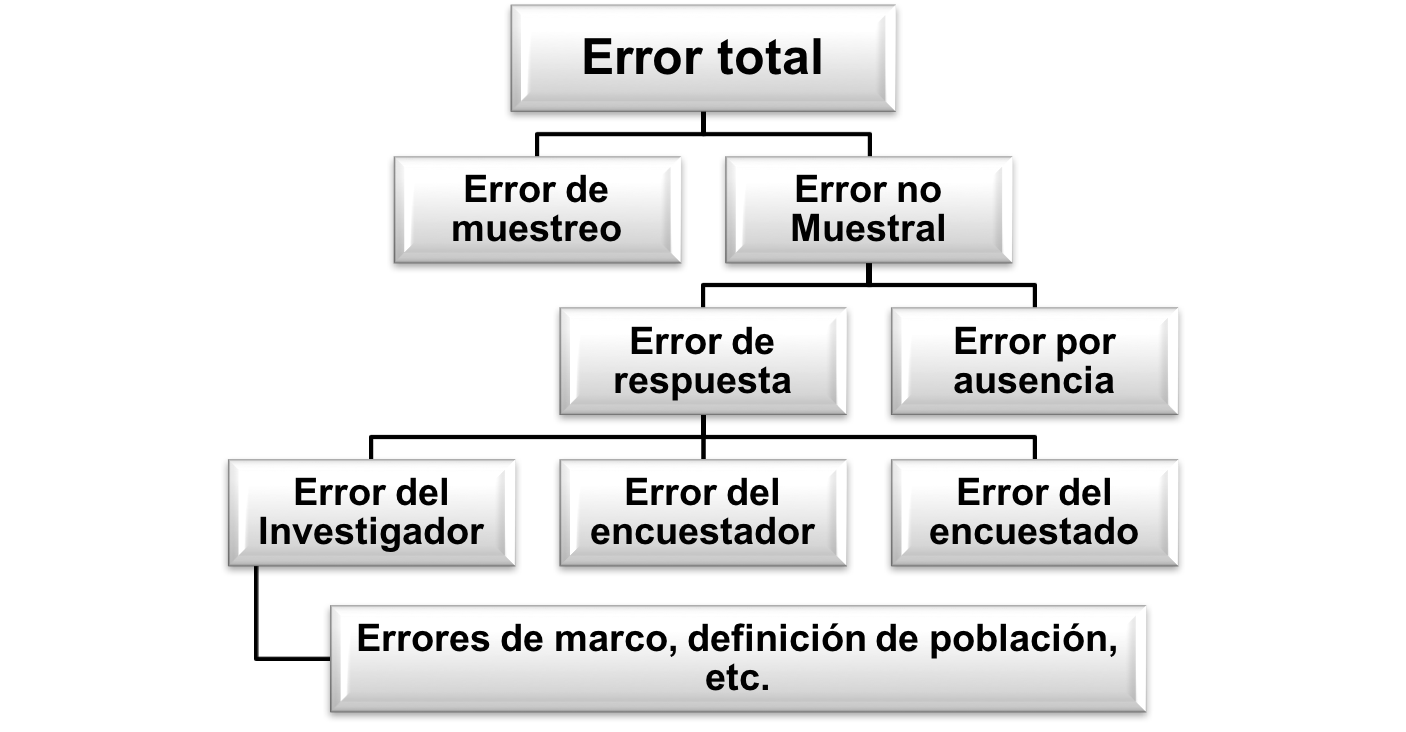
\includegraphics[width=19.53in]{Pics/Picture9} \caption{El paradigma del error total. Fuente: adaptación de Groves et al. (2009)}\label{fig:errortotal}
\end{figure}

Por ejemplo, en una encuesta de fuerza laboral mensual, puede haber confusión en el respondiente si no se hace hincapíe en el periodo de referencia; no es lo mismo indagar por la semana pasada, que por el mes pasado y el respondiente debe ser guiado para evitar equivocaciones. Además pueden existir no respondientes en algún subgrupo de interés, o incluso el marco puede estar desactualizado. Uno de los objetivos de la planeación concienzuda de la encuesta es minimizar los errores no muestrales. Es necesario minimizar las discrepancias encontradas entre la respuesta verdadera a una pregunta y la respuesta final.

\citet{Groves_Fowler_Couper_Lepkowski_Singer_Tourangeau_2009} plantea que durante todo el siglo pasado, ha surgido una serie de teorías y principios que ofrecen un marco de referencia unificado en el diseño, implementación y evaluación de encuestas. Este marco de referencia se conoce comúnmente como el paradigma del error total de muestreo y ha encaminado la investigación moderna hacia una mejor calidad de las encuestas.

\hypertarget{sesgos-generados-en-las-encuestas}{%
\section{Sesgos generados en las encuestas}\label{sesgos-generados-en-las-encuestas}}

\citet{Gutierrez_2016} plantea que existen diferentes fuentes de sesgo en las encuestas y resume de la siguiente forma las dos fuentes de sesgo más importantes:

\hypertarget{sesgo-de-selecciuxf3n}{%
\subsection{Sesgo de selección}\label{sesgo-de-selecciuxf3n}}

Este tipo de sesgo ocurre cuando parte de la población objetivo no está en el marco de muestreo, o cuando el marco está incompleto y presenta deficiencias. Por ejemplo, una muestra a conveniencia\footnote{A pesar de que las muestras por conveniencia o por juicio no pueden ser utilizadas para estimar parámetros de la población, éstas sí pueden proporcionar información valiosa en las primeras etapas de una investigación o cuando no es necesario generalizar los resultados a la población.} es sesgada pues las unidades más fáciles de elegir o las que más probablemente respondan a la encuesta no son representativas de las unidades más difíciles de elegir. \citet{Loh} afirma que se presenta este tipo de sesgo si:

\begin{itemize}
\tightlist
\item
  La selección de la muestra depende de cierta característica asociada a las propiedades de interés. Por ejemplo: si la encuesta se realiza ingresando a un portal web, y precisamente las personas que no tienen cobertura de internet difieren significativamente de quienes sí tienen acceso.
\item
  La muestra se realiza mediante elección deliberada o mediante un juicio subjetivo. Por ejemplo, si el parámetro de interés es la cantidad promedio de gastos en compras en un centro comercial y el encuestador elige a las personas que salen con muchos paquetes, entonces la información estaría sesgada puesto que no está reflejando el comportamiento promedio de las compras.
\item
  Existen errores en la especificación de la población objetivo. Por ejemplo, en encuestas electorales, cuando la población objetivo contiene a personas que no están registradas como votantes ante la organización electoral de su país.
\item
  Existe sustitución deliberada de unidades no disponibles en la muestra. Si, por alguna razón, no fue posible obtener la medición y consecuente observación de la característica de interés para algún individuo en la población, la sustitución de este elemento debe hacerse bajo estrictos procedimientos estadísticos y no debe ser subjetiva en ningún modo.
\item
  Existe ausencia de respuesta. Este fenómeno puede causar distorsión de los resultados cuando los que no responden a la encuesta difieren críticamente de los que si respondieron.
\item
  La muestra está compuesta por respondientes voluntarios. Los foros radiales, las encuestas de televisión y los estudios de portales de internet no proporcionan información confiable.
\end{itemize}

Además de lo anterior, en América Latina pueden existir sesgos ocasionados por la falta de cobertura en el marco de muestreo, o por la exclusión planificada de subpoblaciones de difícil acceso. Por ejemplo, en una encuesta de fuerza de trabajo, es posible que la encuesta no sea representativa de las subpoblaciones afrodescendientes o indígenas, por no cubrir exhaustivamente los territorios donde se ubican.

\hypertarget{sesgo-de-mediciuxf3n}{%
\subsection{Sesgo de medición}\label{sesgo-de-mediciuxf3n}}

Este tipo de sesgo ocurre cuando el instrumento con el que se realiza la medición tiene una tendencia a diferir del valor verdadero que se desea averiguar. Este sesgo debe ser considerado y minimizado en la etapa de diseño de la encuesta. Si el instrumento de medición (cuestionario) tiene defectos en su planificación, entonces el resultado de la estimación en la encuesta seguramente diferirá sistemáticamente del verdadero valor para cada uno de los respondientes. Ningún análisis estadístico podrá ajustar esta diferencia sistemática. \citet{Loh} cita algunas situaciones en donde se presenta este sesgo de medición:

\begin{itemize}
\tightlist
\item
  Cuando el respondiente miente. Esta situación se presenta a menudo en encuestas que preguntan acerca del ingreso salarial, alcoholismo y drogadicción, nivel socioeconómico e incluso edad.
\item
  Cuando el cuestionario contiene preguntas difíciles de comprender. Por ejemplo: \emph{``¿No es cierto que usted no recibe remesas desde el exterior?''} La doble negación en esta pregunta es muy confusa para el respondiente.
\item
  Cuando hay un olvido del respondiente que no permite tener una respuesta veráz. Las personas tienden a olvidar, sobretodo las malas experiencias; esta situación debe acotarse si se está trabajando en una encuesta de criminalidad, victimización, consumo de sustancias psicoactivas, o módulos con preguntas sensibles.
\item
  Cuando se brindan distintas respuestas a diferentes entrevistadores. En algunas regiones es muy probable que la raza, edad o género del encuestador afecte directamente la respuesta del entrevistado.
\item
  Cuando se leen mal las preguntas o se polemiza con el respondiente. El encuestador puede influir notablemente en las respuestas. Por lo anterior, es muy importante que el proceso de entrenamiento del entrevistador sea riguroso y completo.
\item
  Cuando la muestra está compuesta por respondientes voluntarios. Los foros radiales, las encuestas de televisión y los estudios de portales de internet no proporcionan, en general, información confiable. En este caso también se presenta sesgo de selección.
\end{itemize}

\hypertarget{evoluciuxf3n-de-las-encuestas-estandarizadas}{%
\section{Evolución de las encuestas estandarizadas}\label{evoluciuxf3n-de-las-encuestas-estandarizadas}}

Cuando el mundo occidental superó los grandes traumatismos del siglo XX (dos guerras mundiales y una recesión a larga escala), la investigación social tuvo un auge sobresaliente a través de las encuestas por correo postal. Según lo comenta el \citet{INE2012}, en el caso Latinoamericano, la Agencia para el Desarrollo Internacional (AID) auspició la serie de catorce documentos ``Atlántida: Un Estudio de Caso en Encuesta de Hogares por Muestra'' (\citet{Atlantida}), elaborado por la Ofician de Censos los Estados Unidos de América, en el marco del Programa Alianza para el Progreso y presentado en colaboración con la Organización de Estados Americanos (OEA) y el Instituto Interamericano de Estadística. A partir de Atlántida se insituyó un modelo que serviría de apoyo para la realización de las encuestas de hogares en América Latina.

Desde el momento en que las encuestas de hogares se instauraron como un instrumento apropiado para la investigación, existen tres preguntas, en continua dinámica, que se deben responder para planificar, ejecutar y analizar una encuesta: ¿cómo se diseñarán las preguntas? ¿cómo se seleccionará la muestra? y ¿cómo se recolectarán las respuestas?

\hypertarget{inicio-de-los-cuestionarios-estandarizados}{%
\subsection{Inicio de los cuestionarios estandarizados}\label{inicio-de-los-cuestionarios-estandarizados}}

La práctica de realizar las mismas preguntas en forma de cuestionario es relativamente reciente. Antes de acoger un proceso estandarizado, cada encuestador podría preguntar ``lo mismo'', pero con diferentes palabras. Difícilmente, dos personas distintas eran entrevistadas con las mismas preguntas. \citet{Groves_Fowler_Couper_Lepkowski_Singer_Tourangeau_2009} mencionan que la forma en cómo se preguntaba y cómo se recopilaba la información afectaba dramáticamente los resultados de las encuestas. Fue así como se decidió que los encuestadores deberían ser entrenados formalmente.

Desde la psicometría se implementó el formalismo del cuestionario. Intentando medir estados psicológicos, afectivos e intelectuales, se desarrollaron técnicas apropiadas para hacer comparables las respuestas. \citet{Likert_1932} demostró que era posible realizar este tipo de comparaciones, evadiendo los largos instrumentos de medición, al formular una sola pregunta - a todos los encuestados - con una serie de respuestas en forma de escala.

\hypertarget{inicio-de-los-muxe9todos-de-muestreo}{%
\subsection{Inicio de los métodos de muestreo}\label{inicio-de-los-muxe9todos-de-muestreo}}

En un principio, los investigadores trataban de recolectar datos sobre todos los elementos de la población de interés. Esta práctica resultaba logísticamente inadecuada cuando se trataba de poblaciones con un gran tamaño. Los cálculos de los indicadores sobre toda una población resultaban muy demandantes. \citet{Groves_Fowler_Couper_Lepkowski_Singer_Tourangeau_2009} afirman que, aunque la teoría de la probabilidad tuvo sus orígenes en el siglo XVIII, no fue hasta la segunda década del siglo XX que se utilizó para realizar encuestas. La primera aplicación fue la selección sistemática de un elemento en una población enlistada. Para realizar esta selección, los registros censales se dividían en secciones y se procedía a seleccionar un elemento de la sección.

Más adelante, cuando la estadística permeó la agricultura, se definieron otros tipos de muestreo (menos demandantes) y se dio origen al muestreo de áreas. Es así como hoy en día es posible seleccionar muestras de bloques, zonas amanzanadas, secciones y sectores cartográficos, o áreas de empadronamiento censal. Se descubrió que era posible generalizar el muestreo de áreas y se creó el muestreo multietápico que permitió la selección de grandes bloques dentro de una ciudad, y áreas dentro de los bloques y el submuestreo sucesivo de unidades dentro hasta llegar a la unidad de interés. Todos estos submuestreos se realizan de forma probabilística.

La gran depresión en EE.UU. y la segunda guerra mundial fueron catalizadores de las encuestas a gran escala, puesto que en ese entonces, al igual que hoy, la tasa de desempleo era una cifra importante para la economía de los países. Por ende, las políticas públicas empezaron a decidirse de acuerdo con las estadísticas oficiales, puesto que las grandes encuestas empezaron a realizarse con una periodicidad mensual. Hoy en día existen cientos de encuestas mensuales que dan cuenta de la realidad de las sociedades en la región.

\hypertarget{inicio-de-la-recolecciuxf3n-de-datos}{%
\subsection{Inicio de la recolección de datos}\label{inicio-de-la-recolecciuxf3n-de-datos}}

Debido a que en un principio no existía un cuestionario estandarizado, entonces las respuestas abiertas eran la única opción de recopilar información. Esta práctica demandaba un gran esfuerzo en términos de resumir y sintetizar todo el corpus de palabras que los entrevistados usaban para responder.

En la mitad de la década del sesenta del siglo pasado, empezó una proliferación masiva de las entrevistas por correo en EE. UU. Los países con registros administrativos actualizados pueden contemplar este escenario puesto que induce altas tasas de cobertura a precios más económicos (pues se prescinde del encuestador). Las bajas tasas de respuestas (pues el encuestado debe llenar un formulario con sus respuestas y devolverlo a la oficina postal) hicieron que paulatinamente esta forma de recolección no fuese tan apetecida \citep{Groves_Fowler_Couper_Lepkowski_Singer_Tourangeau_2009}.

Como lo señala \citet{CEPALcuadernos}, en el caso latinoamericano en la primera parte del decenio de 1960 varios países de América Latina comenzaron a realizar encuestas de hogares periódicas con el propósito de obtener información sobre empleo y desempleo. En 1965 se realizó en la ciudad de México un seminario en que se presentó el estudio de Atlántida. Luego, ante la necesidad de satisfacer la demanda de información en relación con las políticas económicas y sociales, tomó gran impulso en varios países de la región la puesta en marcha de programas permanentes de encuestas de hogares dirigidos fundamentalmente a obtener información sobre la fuerza de trabajo. El modelo Atlántida se basó fundamentalmente en un modelo de encuesta empleado en países desarrollados que tienen mercado de trabajo con características propias. Sin embargo, resultó sumamente interesante para aquellos países que tenían poca experiencia en encuestas de hogares, y constituyó la base metodológica sobre la que se han establecido gran parte de las encuestas
de América Latina (\citet{CEPALcuadernos}).

Un camino intermedio entre la recolección de información presencial (cara a cara) y la recolección de información mediante formularios auto-administrados (por correo electrónico, mediante páginas de internet o mediante correo postal) son las entrevistas telefónicas. Hoy en día, la mayoría de sondeos en investigación de medios y de mercado se realiza por teléfono. Más aún, a partir de la pandemia por COVID-19, en marzo del 2020 el mundo sufrió una paralización de las actividades sociales y económicas, debido a los esfuerzos de los gobiernos para tratar de frenar la expansión de la pandemia en los países. Fue así como, debido a las restricciones de movilidad impuestas por los gobiernos, las operaciones estadísticas con levantamiento de datos presencial fueron suspendidas. En América Latina el rigor de la pandemia y de las medidas de restricción a la movilidad también afectaron el levantamiento de las encuestas de hogares. Sin embargo, a partir de estas dificultades \citet{CEPAL_continua} recomendó la continuidad de las encuestas mediante el uso de entrevistas telefónicas.

\hypertarget{el-ciclo-de-vida-de-una-encuesta}{%
\section{El ciclo de vida de una encuesta}\label{el-ciclo-de-vida-de-una-encuesta}}

Atendiendo al modelo de \citet{Groves_Fowler_Couper_Lepkowski_Singer_Tourangeau_2009}, se puede afirmar que en todas la encuestas se tienen dos niveles de inferencia: el individual y el grupal (Figura \ref{fig:figinferencias}). El proceso de inferencia individual trata con los mismos respondientes que proveen la información primaria en el estudio; mientras que el el proceso de inferencia grupal, basado en una aproximación inductiva, va desde lo particular (la muestra) a lo general (la población).

\begin{figure}
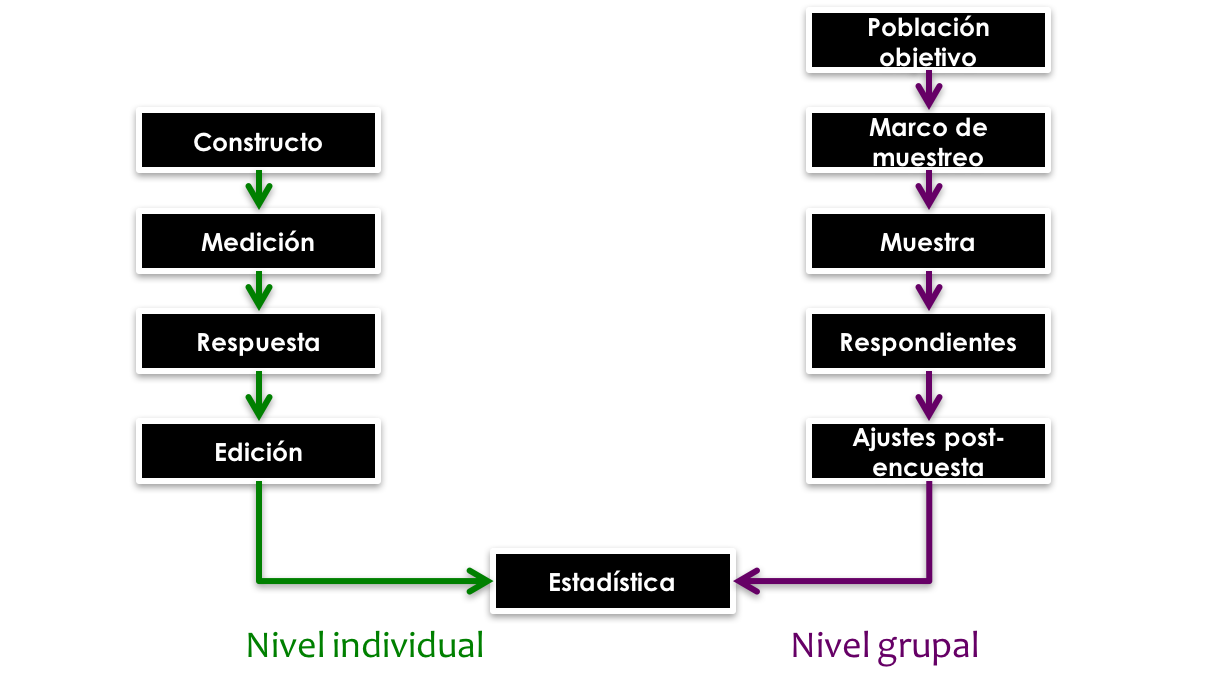
\includegraphics[width=17.03in]{Pics/Picture6} \caption{Dos niveles de inferencia en una encuesta. Fuente: adaptación de Groves et al. (2009)}\label{fig:figinferencias}
\end{figure}

\hypertarget{inferencia-individual}{%
\subsection{Inferencia individual}\label{inferencia-individual}}

\hypertarget{constructo}{%
\subsubsection{Constructo}\label{constructo}}

\citet{Gutierrez_2016} menciona que los constructos son las ideas abstractas (ambiguas) sobre las cuales el investigador desea inferir y que, a su vez, dan origen a la investigación al ser la simiente de la encuesta. Las palabras con que se describen los constructos son siempre simples, pero la redacción elaborada de los constructos no siempre es precisa. Por ejemplo:

\begin{itemize}
\tightlist
\item
  En una \emph{encuesta de victimización} que mida la cantidad de incidentes relacionados con crímenes en un año determinado, es necesario definir muy apropiadamente qué se entiende por crimen, o cómo se define a una víctima, entre otros muchos aspectos.
\item
  En una \emph{encuesta de goce efectivo de derechos ciudadanos} sobre menores de edad se puede medir la efectividad del Estado al garantizar los derechos básicos a la primera infancia. Sin embargo, es necesario definir qué es un derecho, o cómo se define primera infancia.
\end{itemize}

Mientras que algunos constructos son más abstractos que otros (optimismo en la economía, confianza inversionista, percepción del Plan Nacional de Desarrollo de un gobierno), algunos otros son observables más concretamente (consumo de alcohol y otras drogas, nutrición en la primera infancia, productividad de una intervención en el sector agrícola, factores de riesgo asociados a una enfermedad).

\hypertarget{mediciones}{%
\subsubsection{Mediciones}\label{mediciones}}

La medición es una caracterización mucho más concreta que el constructo, puesto que representa una forma de obtener información de los constructos de interés. La cuestión clave para realizar una buena medición es realizar preguntas que induzcan respuestas que reflejen claramente los constructos que se desean medir. \citet{Groves_Fowler_Couper_Lepkowski_Singer_Tourangeau_2009} indican que estas preguntas pueden ser comunicadas en forma oral (encuestas cara a cara o telefónicas), o comunicadas en forma visual (atributos de un producto - marketing). Así mismo, también pueden existir observaciones directas del encuestador (condiciones de la vivienda), u observaciones provenientes de dispositivos electrónicos o físicos (precios de productos en supermercados, muestra de agua, muestra de sangre, etc.).

\hypertarget{respuesta-y-ediciuxf3n}{%
\subsubsection{Respuesta y edición}\label{respuesta-y-ediciuxf3n}}

El resultado de la medición es la respuesta y sus propiedades están determinadas por la naturaleza de las preguntas. Después de que los entrevistados han respondido, los datos deben pasar por un proceso de edición y validación de inconsistencias.

En este proceso de edición se debe examinar la distribución completa de las respuestas y buscar \emph{datos atípicos} para que sean revisados con detenimiento. Los datos editados constituyen el insumo para realizar todo el proceso de inferencia estadística pertinente para que las cifras resultantes sean confiables y precisas.

\hypertarget{inferencia-grupal}{%
\subsection{Inferencia grupal}\label{inferencia-grupal}}

\hypertarget{la-poblaciuxf3n-objetivo}{%
\subsubsection{La población objetivo}\label{la-poblaciuxf3n-objetivo}}

De las definiciones concernientes a agregados, esta es la más abstracta. En general, la \emph{población objetivo} representa el conjunto de unidades que serán estudiadas. Por ejemplo, en una encuesta es posible definir la población objetivo como los adultos nacionales. Sin embargo, esta definición de población no contempla el periodo de referencia de la medición, tampoco aclara si se incluyen los adultos residentes en el exterior y, no precisa cómo se verificará la nacionalidad de un entrevistado.

Por ende, la definición de la población objetiva tiene que ser lo más precisa posible. Por ejemplo, la Gran Encuesta Integrada de Hogares de Colombia define a su población objetivo como la Población civil no institucionalizada (PCNI), la cual contiene a todas las personas que no hacen parte de la fuerza pública y no pertenecen a instituciones de aislamiento como prisiones, hospitales, sanatorios, ancianatos, etc. La PCNI contiene a la población en edad de trabajar (PET) y a los no pertenecientes a la fuerza laboral. La edad para empezar a trabajar en el área rural es 10 años, y en la ciudad es 12 años. A su vez, la PET contiene a Inactivos y Ocupados. La clasificación de ocupado es una variable derivada que está inducida por muchos filtros.

\hypertarget{la-poblaciuxf3n-enmarcada}{%
\subsubsection{La población enmarcada}\label{la-poblaciuxf3n-enmarcada}}

No es posible realizar una encuesta probabilística sin un \emph{marco de muestreo}, definido como un dispositivo que permite ubicar e identificar (ambas acciones al mismo tiempo) las unidades pertenecientes a la población de interés. En América Latina, es a partir del censo que se construyen los marcos de muestreo para las encuestas de hogares en los países, miestras que en algunos países desarrollados es posible encontrar marcos de muestreo creados a partir de líneas telefónicas o dirección de residencia.

Es necesario darse cuenta de que todos los marcos de muestreo presentan algún nivel de desactualización con respecto a la población de interés. Por ejemplo, un marco de muestreo de áreas (basado en la cartografía del último ejercicio censa) puede estar desactualizado. Asimismo, algunas posibilidades negativas del uso de este tipo de marcos es que es posible entrevistar a la misma persona en varias ocasiones (si la persona tiene múltiples residencias), o incluso nunca realizar la entrevista a una persona que no tienen un lugar fijo de residencia. Por otra lado, un marco de muestreo de líneas telefónicas puede no contener a todos lo residentes de una ciudad.

La población enmarcada está definida por el conjunto de miembros de la población objetivo que efectivamente tienen una probabilidad no nula de ser seleccionados en una muestra probabilística. En general para definir quién pertenece a un hogar del marco existen dos alternativas:

\begin{enumerate}
\def\labelenumi{\arabic{enumi}.}
\tightlist
\item
  Regla \emph{de iure}: quien habitualmente reside en el hogar es miembro de ese hogar.

  \begin{itemize}
  \tightlist
  \item
    Una situación \emph{de iure} es aquella que está reconocida por la legalidad vigente o por la autoridad competente en virtud de algún acuerdo o acto formal.
  \item
    Evita la subcobertura de individuos que no residen usualmente en su hogar, considerándolo suyo.
  \end{itemize}
\item
  Regla \emph{de facto}: quien pasó la noche anterior en una residencia de un hogar es miembro de ese hogar.

  \begin{itemize}
  \tightlist
  \item
    Una situación \emph{de facto} es aquella que, existiendo en la realidad, no ha sido reconocida formalmente.
  \item
    Evita la sobrecobertura de individuos que tienen más de una residencia.
  \end{itemize}
\end{enumerate}

\hypertarget{la-muestra}{%
\subsubsection{La muestra}\label{la-muestra}}

El tamaño de muestra define directamente la precisión y confiabilidad de las estimaciones. Este debería incrementarse a medida que lo hagan los niveles de desagregación (grupos etarios, regiones geográficas, niveles de escolaridad, etc.). Sin embargo, dependiendo de la caracterización de la estrategia de muestreo, pueden existir escenarios en donde una encuesta con un tamaño de muestra menor induzca menores errores de muestreo que una encuesta con un mayor tamaño de muestra.

No obstante, en algunas ocasiones los esfuerzos realizados para que los individuos seleccionados en la muestra respondan no son fructíferos. De esta manera, los individuos que son efectivamente entrevistados se denominan respondientes efectivos; mientras que al complemento de este conjunto se les denomina no respondientes.

\hypertarget{los-respondientes}{%
\subsubsection{Los respondientes}\label{los-respondientes}}

Pueden existir casos de no respondientes parciales (no respondientes de ítems), para los cuales debe existir un proceso de \emph{decisión} en términos de su reemplazo. Asimismo, no todas las ausencias parciales son reemplazadas. \citet{Groves_Fowler_Couper_Lepkowski_Singer_Tourangeau_2009} afirman que algunos de los factores que inciden en el aumento de la ausencia de respuesta pueden ser causados por:

\begin{itemize}
\tightlist
\item
  \emph{Contenido}: por preguntas sensibles (encuestas relacionadas con el uso de drogas, finanzas, victimización). En este caso, se puede acotar la tasa de respuesta si se ordenan las preguntas de manera adecuada.
\item
  \emph{Encuestadores}: aplicar métodos estándar de mejoramiento de la calidad para aumentar la precisión y tasa de respuesta de los entrevistadores involucrados en el estudio.
\item
  \emph{Método de recolección}: las encuestas telefónicas, por correo electrónico o por páginas web tienen una tasa de respuesta menor que las entrevistas personales.
\item
  \emph{Diseño de cuestionario}: mala planificación en el pase de las preguntas que conforman el instrumento.
\item
  \emph{Tiempo de la encuesta y agobio}: algunas temporadas arrojan tasas de no respuestas más altas que otras. De la misma forma, algunos cuestionarios largos son propensos a inducir una mayor ausencia de respuesta parcial por el agotamiento del respondiente. En general, las encuestas demasiado largas pueden indisponer al respondiente.
\end{itemize}

\hypertarget{los-ajustes-post-encuesta}{%
\subsubsection{Los ajustes post-encuesta}\label{los-ajustes-post-encuesta}}

Toda encuesta cuenta con personas que no quisieron responder y/o con un marco de muestreo que no cubre a toda la población. Por ende, es necesario realizar algunos ajustes en el análisis y procesamiento para evitar, sobretodo, la sub-estimación de los parámetros de interés, o implementar métodos de imputación para suplir la información faltante. De esta forma se puede utilizar una reponderación diferencial cuando es evidente que hay un patrón de ausencia de respuesta en algunos subgrupos de la población; por ejemplo: si las tasas de respuestas a nivel urbano son menores que las tasas de respuesta a nivel rural, o si los hombres responden menos que las mujeres.

También es posible imputar (cuya raíz inglesa es \emph{input}, traducido como introducir valores) los valores perdidos en un subconjunto de observaciones de la muestra seleccionada. En este caso es factible utilizar metodologías estocásticas complejas para imputar valores, o técnicas simples sistemáticas. Sin embargo, en cualquier caso, siempre es preferible obtener la respuesta directa del entrevistado.

\hypertarget{el-proceso-de-respuesta}{%
\section{El proceso de respuesta}\label{el-proceso-de-respuesta}}

No todas las encuestas se planean de tal forma que exista una interacción directa entre respondiente y entrevistador en todo tiempo. Sin emabrgo los modelo de respuesta en las encuestas asumen que existen, por lo menos, lo siguientes momentos en la obtención de un valor numérico que se recopila como respuesta al cuestionario:

\begin{enumerate}
\def\labelenumi{\arabic{enumi}.}
\tightlist
\item
  \emph{La comprensión}, momento en donde el respondiente interpreta la pregunta. \citet{Groves_Fowler_Couper_Lepkowski_Singer_Tourangeau_2009} afirman que en este momento se involucran todos aquellos procesos de atención a la pregunta y entendimiento de las instrucciones. La primera tarea del respondiente es interpretar la pregunta y, al hacerlo surgen procesos de análisis y asignación de un significado a los elementos sustantivos de la pregunta. Además el respondiente debe hacer una inferencia sobre el propósito de la pregunta, determinar los límites de la respuesta, así como acotar los posibles traslapes sobre las respuestas permitidas.
\item
  \emph{El recaudo}, momento en donde el respondiente recolecta en su memoria la información necesaria para brindar una respuesta. En algunas ocasiones se accede a la memoria de largo plazo que almacena todo el contenido autobiográfico y el conocimiento general. Nótese que muchas cosas pueden afectar el desempeño de la memoria de largo plazo (cuando los eventos en cuestión no se distinguen con facilidad o cuando los eventos no tienen un gran impacto personal). La memoria provee la información relevante para que el entrevistado proporcione una respuesta adecuada. Este ciclo de recaudo de información continúa hasta que el entrevistado dé una respuesta acertada o simplemente no quiera recordar más (algunas situaciones son más difíciles de recordar) \citep{Groves_Fowler_Couper_Lepkowski_Singer_Tourangeau_2009}. Para ayudar a la memoria de largo plazo se pueden diseñar señales o pistas auto-contenidas en la pregunta. Las mejores señales son las que ofrecen un nivel de detalle más profundo.
\item
  \emph{El juicio}, momento en donde se combina, se pondera y se resume la información recolectada. En esta etapa se surten procesos que complementan los recaudos que el entrevistado ha contemplado anteriormente. El juicio puede llenar los vacíos de la memoria, combinar los recaudos o ajustarlos por omisión. Por ejemplo, en una encuesta de ingresos y gastos, las personas, por lo general, no llevan la cuenta del número de veces que compraron cierto artículo o no tienen una respuesta predefinida al número de veces que han salido de compras. Por ende, el respondiente tratará de contar el número de veces que experimentó una situación, y si ese número es muy grande, seguramente se acercará a la respuesta mediante una estimación. La estrategia de estimación del respondiente (llevar la cuenta, construir una escala mediante la recordación de eventos, realizar una estimación gruesa o adivinar al azar) depende del número de sucesos, su duración, la regularidad de los mismos y el periodo de referencia de la encuesta \citep{Groves_Fowler_Couper_Lepkowski_Singer_Tourangeau_2009}.
\item
  \emph{El reporte}, momento en donde el respondiente formula su respuesta y la estandariza en el formato inducido por el cuestionario. Este es el proceso de selección y comunicación de una respuesta, que incluye el encuadre de la respuesta dentro de las opciones que provee la pregunta (también implica alterar la respuesta para que se ajuste a las opciones aceptables). La forma en que se reporta la respuesta final dependerá del ajuste que se realice en los procesos de recaudo y estimación y las restricciones que la pregunta impone. En este sentido, si para una pregunta de percepción la mayoría de opciones de respuesta son negativas, la respuesta estará sesgada en esa dirección. Asimismo, los respondientes pueden dar mayor importancia a ciertas opciones de respuesta \citep{Groves_Fowler_Couper_Lepkowski_Singer_Tourangeau_2009}.
\end{enumerate}

El investigador debe saber que el solo hecho de haber experimentado una situación, no implica que el respondiente haya compilado la suficiente información para reportarla como respuesta. \citet{Groves_Fowler_Couper_Lepkowski_Singer_Tourangeau_2009} afirman que se ha visto que los testigos presenciales de una situación omiten detalles importantes acerca de la situación de la cual son testigos. Además, las personas no pueden proveer la información que no tienen. Si la gente no compila la información necesaria, ninguna pregunta ni formulación logrará obtener la respuesta real. Por lo que se recomienda llevar a cabo las pruebas necesarias para validar el cuestionario. Por otro lado, aunque el respondiente conozca con exactitud la respuesta a una pregunta, no será capaz de reportarla correctamente si no hay una buena interpretación de la misma.

Por otra parte, es necesario advertir que la respuesta del entrevistado también está supeditada a los tiempos de ocurrencia (los eventos que sucedieron hace mucho tiempo son más difíciles de recordar), a los límites temporales y su correspondiente impacto emocional, puesto que los eventos cercanos a momentos que generan impacto emocional son más fáciles de recordar (eventos catastróficos, atentados terroristas o desastres naturales) y también a las señales en las preguntas, pues la asignación de múltiples señales en la redacción de la pregunta ayuda a activar el proceso de recordación.

En cuanto a la naturaleza de las preguntas, se puede notar que las preguntas cerradas con escala ordenada podrían tender a producir un sesgo de respuesta positivo, pues los respondientes tienden a evadir las opciones negativas de la escala (encuestas de satisfacción). \citet{Schwarz1991} demostró que las etiquetas numéricas afectan el proceso de respuesta, por lo cual recomendó que el encuestador no lea los números en las opciones de respuesta, así como acotar el número de opciones en preguntas de opinión (no muy pocas, no tantas).

Así mismo, nótese que la generación de pocas opciones de respuesta hace que se pierda el poder de discriminación, mientras que utilizar muchas opciones puede hacer que los encuestados no distingan fácilmente entre las categorías adyacentes. Además, es posible que el respondiente no quiera esperar a que el entrevistador lea exhaustivamente todas las opciones de respuesta. En este caso se presentan dos fenómeno que es necesario evadir. En primer lugar el efecto de primacía, el cual incrementa el riesgo de que el respondiente escoja una de las primeras opciones; y el efecto de recencia, en donde el respondiente siempre escogerá una de las últimas opciones.

Algunos respondientes podrán desviarse del modelo de respuesta mediante la escogencia de rutas alternas de evasión (el encuestado hará el mínimo esfuerzo para satisfacer las demandas del entrevistador). Es así como podríamos encontrar respondientes que seleccionan sistemáticamente las opciones \emph{No sabe} o \emph{No responde}, o que escogen siempre la misma opción para cada pregunta. Inclusive, dependiendo de la apariencia del entrevistador, el respondiente puede estar sesgado a siempre estar de acuerdo (aquiescencia). De la misma manera, es posible que el respondiente quiera presentarse a sí mismo de manera favorable, omitiendo sus atributos no deseables \citep{Groves_Fowler_Couper_Lepkowski_Singer_Tourangeau_2009}.

\hypertarget{elementos-estaduxedsticos-buxe1sicos-en-la-planeaciuxf3n-de-las-encuestas}{%
\chapter{Elementos estadísticos básicos en la planeación de las encuestas}\label{elementos-estaduxedsticos-buxe1sicos-en-la-planeaciuxf3n-de-las-encuestas}}

El fortalecimiento continuo de las investigaciones sociales es un objetivo que los institutos nacionales de estadística procuran cumplir de forma sistemática. En el caso de aquellas operaciones que conllevan la recolección de información primaria y que involucran la selección y medición de hogares y sus miembros, mantener una documentación adecuada que describa las razones por las cuales se ha optado por cierta metodología de recolección en particular es un requisito fundamental para cumplir este cometido. En este apartado se exploran diferentes métodos de recolección de la información y se discuten las diferentes particularidades en la planeación de una encuesta de hogares.

\hypertarget{universo-muestra-y-unidades}{%
\section{Universo, muestra y unidades}\label{universo-muestra-y-unidades}}

El término encuesta se encuentra directamente relacionado con una población finita compuesta de individuos a los cuales es necesario observar y medir. Este proceso es realizado por medio de una entrevista presencial, telefónica o mediante formularios electrónicos autoadministrados. El conjunto de unidades de interés recibe el nombre de \emph{población objetivo} o \emph{universo} y sobre ellas se obtiene la información de interés para el estudio. Por ejemplo, \emph{la Encuesta Nacional de Empleo y Desempleo} de Ecuador define su población objetivo como todas las personas mayores de 10 años residentes en viviendas particulares en Ecuador \citep{INEC-EC}.

Las \emph{unidades de análisis} corresponden a los diferentes niveles de desagregación establecidos para consolidar el diseño de la encuesta y sobre los que se presentan los resultados de interés. En México, la \emph{Encuesta Nacional de Ingresos y Gastos de los Hogares} define como unidades de análisis el ámbito al que pertenece la vivienda: urbano alto, complemento urbano y rural. Por otro lado, la \emph{Gran Encuesta Integrada de Hogares} de Colombia tiene cobertura nacional y sus unidades de análisis están definidas por trece grandes ciudades junto con sus áreas metropolitanas \citep{DANE-COL_2017}.

Como se explicará más adelante, es muy difícil contar con una lista actualizada de todos los hogares del país; por lo tanto, para recolectar la información de la población objetivo, el diseño de una encuesta de hogares en América Latina plantea la necesidad de seleccionar en varias etapas ciertas \emph{unidades de muestreo} que sirven como medio para seleccionar finalmente a los hogares y personas que participarán de la muestra. Cuando se requiere seleccionar personas, se hace necesario seleccionar un subconjunto de zonas geográficas; para cada zona seleccionada, se procede a seleccionar a su vez un subconjunto de secciones cartográficas, que antecede a la selección de hogares. Finalmente, el cuestionario es administrado en cada hogar a un respondiente idóneo, que proporciona la información de todos los integrantes del hogar. Dependiendo de la encuesta, en algunos casos se seleccionan aleatoriamente respondientes individuales dentro del hogar; siendo estas las unidades de observación. Por ejemplo, se puede citar la experiencia de Brasil con la \emph{Pesquisa Nacional por Amostra de Domicilios} que se realiza por medio de una muestra de viviendas en tres etapas: las unidades primarias de muestreo (UPM) son los municipios, mientras que las unidades secundarias de muestreo (USM) son los sectores censales, que conforman una malla territorial definida en el último \emph{Censo Demográfico}. Por último, las unidades finales en ser seleccionadas son las viviendas \citep{IBGE_2014}.

\citet[pág. 105]{Duncan_Kalton_1987} afirman que la composición de la población de interés en las encuestas de hogares cambia durante el tiempo, puesto que lo individuos nacen, mueren, migran, e incluso pasan a ser parte de organizaciones que hacen que pierdan su estatus de elegibilidad como unidades de observación en una encuesta. Nótese que la población objetivo de la mayoría de encuestas de hogares en América Latina se refiere a la población civil excluyendo a los miembros de organizaciones militares, personas recluidas en cárceles, personas que se encuentran en hospitales, etc. De igual forma, se debe tener en cuenta que los hogares pueden crearse o desintegrarse rápidamente. Por ende, los equipos técnicos de las ONE que están a cargo del diseño de las encuestas de hogares, que miden de forma transversal a la población de interés, deben tener en cuenta que, aunque los objetivos de la encuesta no cambian en el tiempo, sí lo hace la población objetivo y se deben plantear esquemas de seguimiento y actualización que den cuenta de esta realidad.

\hypertarget{periodicidad-en-el-tiempo}{%
\section{Periodicidad en el tiempo}\label{periodicidad-en-el-tiempo}}

Las Oficinas Nacionales de Estadística - que son los entes encargados de administrar, diseñar, analizar y difundir los resultados de las encuestas - no realizan este tipo de levantamientos de manera aislada; de hecho una característica fundamental de estas operaciones estadísticas es que se han convertido en un insumo fundamental para realizar un seguimiento periódico de muchos indicadores de interés. Por lo tanto, muchas encuestas de hogares se realizan de forma sistemática en el tiempo, aunque algunas otras no tienen una periodicidad predefinida. Es por esto que la planeación de la encuesta debe contemplar este tipo de esquemas continuos para que el levantamiento de la información primaria en campo se haga de manera más eficiente y, de la misma forma, que la estimación de los indicadores de interés se pueda realizar ajustándose a los recursos de la operación. Como se mencionó anteriormente, dado que la población es dinámica en el tiempo, la planeación y análisis de este tipo de encuestas es desafiante, puesto que si la composición de la población y las características de los elementos se considerara fija, una encuesta transversal (realizada una sola vez en un periodo de tiempo largo) sería suficiente para realizar estimaciones precisas que resuelvan los objetivos del estudio.

En algunas ocasiones, basta con realizar un medición simple en un punto específico del tiempo para completar los objetivos de la investigación. Este es el caso de las encuestas de ingresos y gastos cuya periodicidad es, en general, no menor a cinco años y las cuales son utilizadas para, entre muchos otros propósitos, actualizar la canasta básica familiar, de la cual se derivan los insumos básicos para la medición de la pobreza \citep{CEPAL_2018}. Para otro tipo de problemáticas, como por ejemplo el seguimiento a las estadísticas derivadas del mercado de trabajo, es necesario recurrir a la medición periódica a través de encuestas de hogares, en donde los cambios naturales en las características de la población hacen que realizar una medición simple en un punto del tiempo sea insuficiente a la luz del seguimiento y monitoreo de los indicadores de interés.

Por consiguiente, al momento de realizar la planeación de una encuesta continua o periódica se debe tener en cuenta que, a pesar de que crezca la dificultad en el diseño, es posible obtener información más oportuna para la toma de decisiones y la formulación de políticas públicas. De esta manera, y teniendo en cuenta que el tiempo hace que la estructura de las poblaciones cambie, sin importar si la constituyen individuos, hogares, familias, negocios, etc., las unidades de observación deben ser consideradas como parte de la población de interés cuando nacen, inmigran o alcanzan un umbral predefinido de edad. Asimismo, las unidades ya no harán parte de la población de interés cuando mueran, emigren, o se involucren en instituciones (como el servicio militar). Por ejemplo, si las unidades de interés son los hogares, es evidente que la población no es la misma en diferentes puntos del tiempo (por ejemplo, en dos años distintos) puesto que se crean nuevas unidades cuando los jóvenes dejan a sus padres y forman nuevos hogares independientes, o cuando ocurre una separación o un divorcio; en donde un hogar se divide en dos. Además, los hogares en donde todos sus miembros han fallecido dejan de ser parte de la población objetivo. De la misma forma, dos hogares dejan de ser parte de la población objetivo cuando se unen a través de un matrimonio o algún otro tipo de unión civil, formando un nuevo hogar.

Teniendo en cuenta el papel dinámico de las poblaciones y los objetivos de investigación es posible plantear diferentes tipos de levantamientos; a continuación enumeramos algunas categorías de encuestas que las ONE realizan en la región.

\hypertarget{encuestas-transversales}{%
\subsection{Encuestas transversales}\label{encuestas-transversales}}

Este tipo de encuestas son diseñadas para recolectar información únicamente en un punto específico del tiempo, o sobre un periodo de referencia, y proveen toda la información pertinente acerca de la población particular restringida a un tiempo y periodo de recolección específico. Puesto que el propósito fundamental de este tipo de encuestas no se centra en las comparaciones intertemporales, no es posible estimar cambios de ningún tipo, a no ser que se realicen indagaciones retrospectivas. La siguiente tabla muestra un esquema de este tipo de operaciones estadísticas en donde se observa una muestra de una población específica en un periodo de tiempo específico (Tiempo 2). Dado que es una muestra transversal, no hay un patrón de repetición en los restantes periodos.

\begin{longtable}[]{@{}
  >{\centering\arraybackslash}p{(\columnwidth - 12\tabcolsep) * \real{0.1304}}
  >{\centering\arraybackslash}p{(\columnwidth - 12\tabcolsep) * \real{0.1449}}
  >{\centering\arraybackslash}p{(\columnwidth - 12\tabcolsep) * \real{0.1449}}
  >{\centering\arraybackslash}p{(\columnwidth - 12\tabcolsep) * \real{0.1449}}
  >{\centering\arraybackslash}p{(\columnwidth - 12\tabcolsep) * \real{0.1449}}
  >{\centering\arraybackslash}p{(\columnwidth - 12\tabcolsep) * \real{0.1449}}
  >{\centering\arraybackslash}p{(\columnwidth - 12\tabcolsep) * \real{0.1449}}@{}}
\caption{\emph{Esquema de una encuesta transversal.}}\tabularnewline
\toprule()
\begin{minipage}[b]{\linewidth}\centering
Hogar
\end{minipage} & \begin{minipage}[b]{\linewidth}\centering
Tiempo 1
\end{minipage} & \begin{minipage}[b]{\linewidth}\centering
Tiempo 2
\end{minipage} & \begin{minipage}[b]{\linewidth}\centering
Tiempo 3
\end{minipage} & \begin{minipage}[b]{\linewidth}\centering
Tiempo 4
\end{minipage} & \begin{minipage}[b]{\linewidth}\centering
\ldots{}
\end{minipage} & \begin{minipage}[b]{\linewidth}\centering
Tiempo \(T\)
\end{minipage} \\
\midrule()
\endfirsthead
\toprule()
\begin{minipage}[b]{\linewidth}\centering
Hogar
\end{minipage} & \begin{minipage}[b]{\linewidth}\centering
Tiempo 1
\end{minipage} & \begin{minipage}[b]{\linewidth}\centering
Tiempo 2
\end{minipage} & \begin{minipage}[b]{\linewidth}\centering
Tiempo 3
\end{minipage} & \begin{minipage}[b]{\linewidth}\centering
Tiempo 4
\end{minipage} & \begin{minipage}[b]{\linewidth}\centering
\ldots{}
\end{minipage} & \begin{minipage}[b]{\linewidth}\centering
Tiempo \(T\)
\end{minipage} \\
\midrule()
\endhead
1 & & \textbf{x} & & & & \\
2 & & \textbf{x} & & & & \\
3 & & \textbf{x} & & & & \\
4 & & \textbf{x} & & & & \\
\ldots{} & & \textbf{x} & & & & \\
\(n\) & & \textbf{x} & & & & \\
\bottomrule()
\end{longtable}

\hypertarget{encuestas-repetidas}{%
\subsection{Encuestas repetidas}\label{encuestas-repetidas}}

Cuando existe interés en realizar un seguimiento del fenómeno en observación durante el tiempo, se utilizan encuestas repetidas que recolectan información de manera periódica. Este tipo de encuestas proveen información acerca de la dinámica de la composición de la población en el tiempo. De esta forma, en cada levantamiento se observa una muestra de la población en un tiempo determinado. Por ejemplo, la siguiente tabla muestra un acercamiento gráfico a este tipo de encuestas en donde se evidencia el carácter sistemático de estas operaciones estadísticas; además de mostrar que no es posible medir cambios individuales porque las muestras son independientes en el tiempo.

\begin{longtable}[]{@{}
  >{\centering\arraybackslash}p{(\columnwidth - 12\tabcolsep) * \real{0.1304}}
  >{\centering\arraybackslash}p{(\columnwidth - 12\tabcolsep) * \real{0.1449}}
  >{\centering\arraybackslash}p{(\columnwidth - 12\tabcolsep) * \real{0.1449}}
  >{\centering\arraybackslash}p{(\columnwidth - 12\tabcolsep) * \real{0.1449}}
  >{\centering\arraybackslash}p{(\columnwidth - 12\tabcolsep) * \real{0.1449}}
  >{\centering\arraybackslash}p{(\columnwidth - 12\tabcolsep) * \real{0.1449}}
  >{\centering\arraybackslash}p{(\columnwidth - 12\tabcolsep) * \real{0.1449}}@{}}
\caption{\emph{Esquema de una encuesta repetida.}}\tabularnewline
\toprule()
\begin{minipage}[b]{\linewidth}\centering
Hogar
\end{minipage} & \begin{minipage}[b]{\linewidth}\centering
Tiempo 1
\end{minipage} & \begin{minipage}[b]{\linewidth}\centering
Tiempo 2
\end{minipage} & \begin{minipage}[b]{\linewidth}\centering
Tiempo 3
\end{minipage} & \begin{minipage}[b]{\linewidth}\centering
Tiempo 4
\end{minipage} & \begin{minipage}[b]{\linewidth}\centering
\ldots{}
\end{minipage} & \begin{minipage}[b]{\linewidth}\centering
Tiempo \(T\)
\end{minipage} \\
\midrule()
\endfirsthead
\toprule()
\begin{minipage}[b]{\linewidth}\centering
Hogar
\end{minipage} & \begin{minipage}[b]{\linewidth}\centering
Tiempo 1
\end{minipage} & \begin{minipage}[b]{\linewidth}\centering
Tiempo 2
\end{minipage} & \begin{minipage}[b]{\linewidth}\centering
Tiempo 3
\end{minipage} & \begin{minipage}[b]{\linewidth}\centering
Tiempo 4
\end{minipage} & \begin{minipage}[b]{\linewidth}\centering
\ldots{}
\end{minipage} & \begin{minipage}[b]{\linewidth}\centering
Tiempo \(T\)
\end{minipage} \\
\midrule()
\endhead
1 & \textbf{x} & & & & & \\
2 & & \textbf{x} & & & & \\
3 & & & \textbf{x} & & & \\
4 & & & & \textbf{x} & & \\
\ldots{} & & & & & \textbf{x} & \\
\(n\) & & & & & & \textbf{x} \\
\bottomrule()
\end{longtable}

\hypertarget{encuestas-panel}{%
\subsection{Encuestas panel}\label{encuestas-panel}}

Las encuestas en panel están diseñadas para recolectar información periódica sobre la misma muestra en diferentes puntos del tiempo. Por definición, las unidades de muestreo son las mismas en los diferentes periodos de tiempo y, de manera general, se miden las mismas variables en cada levantamiento. Por la caracterización propia de este tipo de encuestas, sí es posible estimar los cambios individuales, así como los cambios netos sobre la población. Sin embargo, como la muestra no cambia en ningún momento del tiempo, las inferencias que se realicen estarán supeditadas a la población de la cual se seleccionó la muestra en un principio (Tiempo 1). Si la población cambia su estructura, no será posible captar este cambio puesto que las inferencias resultantes de este tipo de encuestas no son representativas de la población actual. La siguiente tabla muestra un esquema propio de las encuestas de panel en donde los individuos que fueron seleccionados la primera vez son observados a lo largo del tiempo.

\begin{longtable}[]{@{}
  >{\centering\arraybackslash}p{(\columnwidth - 12\tabcolsep) * \real{0.1304}}
  >{\centering\arraybackslash}p{(\columnwidth - 12\tabcolsep) * \real{0.1449}}
  >{\centering\arraybackslash}p{(\columnwidth - 12\tabcolsep) * \real{0.1449}}
  >{\centering\arraybackslash}p{(\columnwidth - 12\tabcolsep) * \real{0.1449}}
  >{\centering\arraybackslash}p{(\columnwidth - 12\tabcolsep) * \real{0.1449}}
  >{\centering\arraybackslash}p{(\columnwidth - 12\tabcolsep) * \real{0.1449}}
  >{\centering\arraybackslash}p{(\columnwidth - 12\tabcolsep) * \real{0.1449}}@{}}
\caption{\emph{Esquema de una encuesta tipo panel.}}\tabularnewline
\toprule()
\begin{minipage}[b]{\linewidth}\centering
Hogar
\end{minipage} & \begin{minipage}[b]{\linewidth}\centering
Tiempo 1
\end{minipage} & \begin{minipage}[b]{\linewidth}\centering
Tiempo 2
\end{minipage} & \begin{minipage}[b]{\linewidth}\centering
Tiempo 3
\end{minipage} & \begin{minipage}[b]{\linewidth}\centering
Tiempo 4
\end{minipage} & \begin{minipage}[b]{\linewidth}\centering
\ldots{}
\end{minipage} & \begin{minipage}[b]{\linewidth}\centering
Tiempo \(T\)
\end{minipage} \\
\midrule()
\endfirsthead
\toprule()
\begin{minipage}[b]{\linewidth}\centering
Hogar
\end{minipage} & \begin{minipage}[b]{\linewidth}\centering
Tiempo 1
\end{minipage} & \begin{minipage}[b]{\linewidth}\centering
Tiempo 2
\end{minipage} & \begin{minipage}[b]{\linewidth}\centering
Tiempo 3
\end{minipage} & \begin{minipage}[b]{\linewidth}\centering
Tiempo 4
\end{minipage} & \begin{minipage}[b]{\linewidth}\centering
\ldots{}
\end{minipage} & \begin{minipage}[b]{\linewidth}\centering
Tiempo \(T\)
\end{minipage} \\
\midrule()
\endhead
1 & \textbf{x} & \textbf{x} & \textbf{x} & \textbf{x} & \textbf{x} & \textbf{x} \\
2 & \textbf{x} & \textbf{x} & \textbf{x} & \textbf{x} & \textbf{x} & \textbf{x} \\
3 & \textbf{x} & \textbf{x} & \textbf{x} & \textbf{x} & \textbf{x} & \textbf{x} \\
4 & & & & & & \\
\ldots{} & & & & & & \\
\(n\) & & & & & & \\
\bottomrule()
\end{longtable}

\hypertarget{encuestas-de-panel-dividido}{%
\subsection{Encuestas de panel dividido}\label{encuestas-de-panel-dividido}}

Para hacerle frente a las dificultades propias de las encuestas de panel y poder observar tanto los cambios individuales, como los cambios en la estructura de la población, se definen las encuestas de panel dividido. Estas operaciones estadísticas son una combinación del diseño de panel puro y del diseño repetido y su objetivo es realizar inferencias precisas acerca de los cambios de una cohorte a través del tiempo y, al mismo tiempo, del cambio en estructura de la población actual. De esta forma, se realiza el seguimiento continuo, periódico y sistemático de una muestra a través del tiempo, pero en cada levantamiento se incluyen nuevos elementos seleccionados de la población actual. Como se señalará más adelante, este tipo de encuestas cubre con eficiencia la mayoría de indicadores de interés en un estudio de investigación social. La siguiente tabla muestra una caracterización de estos levantamientos que fijan una muestra de panel a lo largo del tiempo, y a la vez que se añaden nuevas observaciones.

\begin{longtable}[]{@{}
  >{\centering\arraybackslash}p{(\columnwidth - 12\tabcolsep) * \real{0.1304}}
  >{\centering\arraybackslash}p{(\columnwidth - 12\tabcolsep) * \real{0.1449}}
  >{\centering\arraybackslash}p{(\columnwidth - 12\tabcolsep) * \real{0.1449}}
  >{\centering\arraybackslash}p{(\columnwidth - 12\tabcolsep) * \real{0.1449}}
  >{\centering\arraybackslash}p{(\columnwidth - 12\tabcolsep) * \real{0.1449}}
  >{\centering\arraybackslash}p{(\columnwidth - 12\tabcolsep) * \real{0.1449}}
  >{\centering\arraybackslash}p{(\columnwidth - 12\tabcolsep) * \real{0.1449}}@{}}
\caption{\emph{Esquema de una encuesta de panel dividido.}}\tabularnewline
\toprule()
\begin{minipage}[b]{\linewidth}\centering
Hogar
\end{minipage} & \begin{minipage}[b]{\linewidth}\centering
Tiempo 1
\end{minipage} & \begin{minipage}[b]{\linewidth}\centering
Tiempo 2
\end{minipage} & \begin{minipage}[b]{\linewidth}\centering
Tiempo 3
\end{minipage} & \begin{minipage}[b]{\linewidth}\centering
Tiempo 4
\end{minipage} & \begin{minipage}[b]{\linewidth}\centering
\ldots{}
\end{minipage} & \begin{minipage}[b]{\linewidth}\centering
Tiempo \(T\)
\end{minipage} \\
\midrule()
\endfirsthead
\toprule()
\begin{minipage}[b]{\linewidth}\centering
Hogar
\end{minipage} & \begin{minipage}[b]{\linewidth}\centering
Tiempo 1
\end{minipage} & \begin{minipage}[b]{\linewidth}\centering
Tiempo 2
\end{minipage} & \begin{minipage}[b]{\linewidth}\centering
Tiempo 3
\end{minipage} & \begin{minipage}[b]{\linewidth}\centering
Tiempo 4
\end{minipage} & \begin{minipage}[b]{\linewidth}\centering
\ldots{}
\end{minipage} & \begin{minipage}[b]{\linewidth}\centering
Tiempo \(T\)
\end{minipage} \\
\midrule()
\endhead
1 & \textbf{x} & \textbf{x} & \textbf{x} & \textbf{x} & \textbf{x} & \textbf{x} \\
2 & \textbf{x} & & & & & \\
3 & & \textbf{x} & & & & \\
4 & & & \textbf{x} & & & \\
5 & & & & \textbf{x} & & \\
\ldots{} & & & & & \textbf{x} & \\
\(n\) & & & & & & \textbf{x} \\
\bottomrule()
\end{longtable}

\hypertarget{encuestas-de-panel-rotativo}{%
\subsection{Encuestas de panel rotativo}\label{encuestas-de-panel-rotativo}}

Mantener una muestra de panel es un proceso costoso desde una perspectiva económica y logística, pero también se debe tener en cuenta el desgaste de la fuente, que tenderá a brindar menos información a medida que avanza el estudio. Además, es evidente que a medida que el tiempo transcurra la propensión a responder será más baja, puesto que el entrevistado se sentirá agotado al ser visitado una y otra vez. Por lo tanto, se definen las encuestas de panel rotativo para poder realizar inferencias parciales - restringidas a periodos de tiempo específicos - del cambio individual y a la vez captar el cambio estructural de la población. Estas encuestas incorporan nuevos elementos de la población y a la vez mantienen elementos comunes con mediciones anteriores. Obviando las dificultades que acarrea la ausencia de respuesta, las encuestas panel definen un traslape completo entre las muestras de dos puntos cualesquiera en el tiempo; sin embargo, en las encuestas rotativas existe un traslape parcial, por lo que se reduce el efecto del desgaste del panel (sobre la población inicial) y el efecto de la pérdida de muestra. Además, la inclusión de nuevos elementos en la muestra provee información pertinente del cambio en la composición estructural de la población. La siguiente tabla ejemplifica el diseño de las encuestas rotativas.

\begin{longtable}[]{@{}
  >{\centering\arraybackslash}p{(\columnwidth - 12\tabcolsep) * \real{0.1304}}
  >{\centering\arraybackslash}p{(\columnwidth - 12\tabcolsep) * \real{0.1449}}
  >{\centering\arraybackslash}p{(\columnwidth - 12\tabcolsep) * \real{0.1449}}
  >{\centering\arraybackslash}p{(\columnwidth - 12\tabcolsep) * \real{0.1449}}
  >{\centering\arraybackslash}p{(\columnwidth - 12\tabcolsep) * \real{0.1449}}
  >{\centering\arraybackslash}p{(\columnwidth - 12\tabcolsep) * \real{0.1449}}
  >{\centering\arraybackslash}p{(\columnwidth - 12\tabcolsep) * \real{0.1449}}@{}}
\caption{\emph{Esquema de una encuesta de panel rotativo.}}\tabularnewline
\toprule()
\begin{minipage}[b]{\linewidth}\centering
Hogar
\end{minipage} & \begin{minipage}[b]{\linewidth}\centering
Tiempo 1
\end{minipage} & \begin{minipage}[b]{\linewidth}\centering
Tiempo 2
\end{minipage} & \begin{minipage}[b]{\linewidth}\centering
Tiempo 3
\end{minipage} & \begin{minipage}[b]{\linewidth}\centering
Tiempo 4
\end{minipage} & \begin{minipage}[b]{\linewidth}\centering
Tiempo 5
\end{minipage} & \begin{minipage}[b]{\linewidth}\centering
Tiempo 6
\end{minipage} \\
\midrule()
\endfirsthead
\toprule()
\begin{minipage}[b]{\linewidth}\centering
Hogar
\end{minipage} & \begin{minipage}[b]{\linewidth}\centering
Tiempo 1
\end{minipage} & \begin{minipage}[b]{\linewidth}\centering
Tiempo 2
\end{minipage} & \begin{minipage}[b]{\linewidth}\centering
Tiempo 3
\end{minipage} & \begin{minipage}[b]{\linewidth}\centering
Tiempo 4
\end{minipage} & \begin{minipage}[b]{\linewidth}\centering
Tiempo 5
\end{minipage} & \begin{minipage}[b]{\linewidth}\centering
Tiempo 6
\end{minipage} \\
\midrule()
\endhead
1 & \textbf{x} & & & & & \\
2 & \textbf{x} & \textbf{x} & & & & \\
3 & \textbf{x} & \textbf{x} & \textbf{x} & & & \\
4 & & \textbf{x} & \textbf{x} & \textbf{x} & & \\
5 & & & \textbf{x} & \textbf{x} & \textbf{x} & \\
6 & & & & \textbf{x} & \textbf{x} & \textbf{x} \\
\ldots{} & & & & & \textbf{x} & \textbf{x} \\
\(n\) & & & & & & \textbf{x} \\
\bottomrule()
\end{longtable}

\hypertarget{rotaciuxf3n-de-paneles}{%
\section{Rotación de paneles}\label{rotaciuxf3n-de-paneles}}

Tal como se describió anteriormente, algunas encuestas de hogares en América Latina permiten que un hogar sea visitado en más de una ocasión con el fin de tener estimaciones precisas acerca de los cambios de estado que el hogar o las personas que lo habitan puedan sufrir. Por ejemplo, un hogar que en un periodo estuvo en condición de pobreza extrema, puede estar en otro periodo en condición de pobreza relativa (no extrema) o inclusive puede pasar a estar fuera de la pobreza; en las encuestas de fuerza laboral, una persona puede pasar de estar empleada en un periodo a desempleada en otro periodo. Estos cambios y la dinámica propia que conllevan son de interés para los investigadores y deben ser contemplados desde una perspectiva más amplia en cuanto a su diseño. Nótese que este tipo de variaciones sobre los individuos necesariamente tiene que ser captada a través de un componente de panel, por lo que las encuestas transversales o repetidas no serían viables para realizar estas estimaciones.

En América Latina hay una gran variedad de encuestas de hogares que utilizan diseños rotativos (ver apéndice). Por ejemplo, la \emph{Encuesta Permanente de Hogares} en Argentina renueva periódicamente el conjunto de hogares que serán entrevistados mediante un esquema\footnote{Un esquema de rotación \(x(y)z\), se define como aquel en donde la vivienda entra al panel por \(x\) periodos, se excluye por los siguientes \(y\) periodos y este patrón se repite \(z\) veces en el tiempo. Nçotese que los periodos pueden ser definidos como meses, o trimestres; además un hogar es visitado un total de \(x \times z\) veces.} de rotación \(2(2)2\) que selecciona a las viviendas para ser entrevistadas en dos periodos consecutivos; luego los siguientes dos periodos esas viviendas salen de la selección, para finalmente volver a ser encuestadas en los siguiente dos periodos \citep{INDEC-AR}. De esta forma, dado que la rotación es trimestral, un hogar es seguido a lo largo de 18 meses y esto permite cumplir con los objetivos de la encuesta. Este esquema induce algunas propiedades interesantes, que pueden ser ejemplificadas usando la siguiente tabla definido para los cuatro trimestres de los años 2016, 2017, 2018 en cuatro grupos de muestra: A, B, C y D.

\begin{itemize}
\tightlist
\item
  Entre el primer y el segundo periodo de medición hay un traslape del 50\% de hogares. En particular, nótese que entre 2016-T1 y 2016-T2, la muestra se conserva en un 50\%, puesto que \(a1\) y \(d1\) se repiten. Esto mismo sucede en cada trimestre del esquema rotacional.
\item
  En el tercer periodo no habrá traslape con el primer periodo. Nótese que entre 2016-T1 y 2016-T3 no existe ningún elemento en común. De la misma manera, entre 2016-T2 y 2016-T4, no existe ningún elemento en común. Este mismo patrón se encuentra a lo largo del esquema rotacional.
\item
  En el cuarto periodo se tendrá un 25\% de traslape con el primer periodo. Nótese, por ejemplo, que entre 2017-T1 y 2017-T4, \(c3\) se repite; de la misma manera, entre 2017-T4 y 2018-T3, \(d4\) se repite.
\item
  Finalmente en el quinto periodo se volverá a tener un 50\% de traslape con respecto al primer periodo. Por ejemplo, 2016-T1 y 2017-T1 comparten el 50\% de la muestra \(a1\) y \(b1\); asimismo, 2017-T1 y 2018-T1 comparten el 50\% de la muestra \(c3\) y \(b3\).
\end{itemize}

\begin{longtable}[]{@{}cccccc@{}}
\caption{\emph{Rotación de paneles en un diseño 2(2)2.}}\tabularnewline
\toprule()
Año & Trimestre & A & B & C & D \\
\midrule()
\endfirsthead
\toprule()
Año & Trimestre & A & B & C & D \\
\midrule()
\endhead
2016 & T1 & \emph{a1} & \emph{b1} & \emph{c1} & \emph{d1} \\
& T2 & \emph{a1} & \emph{b2} & \emph{c2} & \emph{d1} \\
& T3 & \emph{a2} & \emph{b2} & \emph{c2} & \emph{d2} \\
& T4 & \emph{a2} & \emph{b1} & \emph{c3} & \emph{d2} \\
2017 & T1 & \emph{a1} & \emph{b1} & \emph{c3} & \emph{d3} \\
& T2 & \emph{a1} & \emph{b2} & \emph{c4} & \emph{d3} \\
& T3 & \emph{a2} & \emph{b2} & \emph{c4} & \emph{d4} \\
& T4 & \emph{a2} & \emph{b3} & \emph{c3} & \emph{d4} \\
2018 & T1 & \emph{a3} & \emph{b3} & \emph{c3} & \emph{d3} \\
& T2 & \emph{a3} & \emph{b4} & \emph{c4} & \emph{d3} \\
& T3 & \emph{a4} & \emph{b4} & \emph{c4} & \emph{d4} \\
& T4 & \emph{a4} & \emph{b3} & \emph{c5} & \emph{d4} \\
\bottomrule()
\end{longtable}

Otro ejemplo de una encuesta que utiliza rotación de paneles es la \emph{Encuesta Continua de Empleo} de Bolivia que, aplicada por el Instituto Nacional de Estadística, hace uso de una metodología mixta que permite el seguimiento continuo y transversal a la tasa de desempleo y a la tasa de subocupación, así como el seguimiento a los cambios que se presentan entre los periodos de interés (trimestres y semestres), a través del análisis longitudinal de los datos en el sector urbano (pues el diseño no es rotativo en el sector rural, debido a la baja incidencia de desempleo en esta zona). En este esquema rotacional 4(0)1 una vivienda es entrevistada durante cuatro trimestres consecutivos, y luego sale del panel definitivamente. Un ejemplo de este tipo de esquemas se presenta en la siguiente tabla.

\begin{itemize}
\tightlist
\item
  Nótese que entre el primer y el segundo periodo de medición hay un traslape del 75\% de hogares. En particular, entre 2016-T1 y 2016-T2, la muestra se conserva en tres cuartas partes puesto que \(a1\), \(c1\) y \(d1\) se repiten. Esto mismo sucede en cada trimestre del esquema rotacional.
\item
  Por otro lado, entre el primer y el tercer periodo habrá un traslape del 50\%. Nótese que entre 2016-T1 y 2016-T3, la mitad de la muestra se conserva puesto que \(a1\) y \(d1\) se repiten. Este mismo patrón se encuentra a lo largo del esquema rotacional.
\item
  Entre el primer y el cuarto periodo se tendrá un 25\% de traslape. Nótese, por ejemplo, que entre 2017-T1 y 2017-T4, \(a2\) se repite; de la misma manera, entre 2017-T4 y 2018-T3, \(d3\) se repite.
\item
  Finalmente entre el primer y quinto periodo no se tiene ningún tipo de traslape.
\end{itemize}

\begin{longtable}[]{@{}cccccc@{}}
\caption{\emph{Rotación de paneles en un diseño 4(0)1.}}\tabularnewline
\toprule()
Año & Trimestre & A & B & C & D \\
\midrule()
\endfirsthead
\toprule()
Año & Trimestre & A & B & C & D \\
\midrule()
\endhead
2016 & T1 & \emph{a1} & \emph{b1} & \emph{c1} & \emph{d1} \\
& T2 & \emph{a1} & \emph{b2} & \emph{c1} & \emph{d1} \\
& T3 & \emph{a1} & \emph{b2} & \emph{c2} & \emph{d1} \\
& T4 & \emph{a1} & \emph{b2} & \emph{c2} & \emph{d2} \\
2017 & T1 & \emph{a2} & \emph{b2} & \emph{c2} & \emph{d2} \\
& T2 & \emph{a2} & \emph{b3} & \emph{c2} & \emph{d2} \\
& T3 & \emph{a2} & \emph{b3} & \emph{c3} & \emph{d2} \\
& T4 & \emph{a2} & \emph{b3} & \emph{c3} & \emph{d3} \\
2018 & T1 & \emph{a3} & \emph{b3} & \emph{c3} & \emph{d3} \\
& T2 & \emph{a3} & \emph{b4} & \emph{c3} & \emph{d3} \\
& T3 & \emph{a3} & \emph{b4} & \emph{c4} & \emph{d3} \\
& T4 & \emph{a3} & \emph{b4} & \emph{c4} & \emph{d4} \\
\bottomrule()
\end{longtable}

Los diseños de las encuestas de hogares deben tener en cuenta la rotación de los paneles y el número de veces que es visitado un hogar. Esta caracterización depende directamente de los indicadores a los cuales la encuesta debe responder. Por ejemplo, el diseño de rotación debe ser diferente si el interés se centra en indicadores de cambio trimestral, a si se requieren indicadores de cambio anual. Por ejemplo, el diseño 4(0)1 es conveniente si el objetivo está en comparar las estimaciones de la tasa de desocupación el mismo mes entre diferentes años, pero no lo será si se quiere conocer el cambio de estado en la situación del trabajo para las mismas personas en dos meses iguales de diferentes años. Nótese que un aspecto importante en la definición de los esquemas longitudinales radica en el tiempo en el que un hogar pertenecerá al panel. Por supuesto, hay que tener en cuenta que la tasa de ausencia de respuesta y pérdida de muestra por desgaste del respondiente crecerá en la medida en que se le pida a un hogar una participación más duradera en el tiempo.

La definición de los indicadores de interés debe primar sobre el diseño de las encuestas de hogares. Por ejemplo, si el objetivo de la encuesta se centra en la estimación del cambio del indicador en dos periodos de tiempo, entonces el cálculo de la precisión de las estimaciones debe tener en cuenta que las muestras no son independientes y por lo tanto se debe calcular la varianza de la primera ronda, la varianza de la segunda ronda y la correlación entre las dos rondas de interés. Estos tres componentes deben intervenir en el cálculo de los coeficientes de variación, así como en la determinación del tamaño de muestra en cada ronda. En efecto, como lo afirma \citet[pág. 236]{McLaren_Steel_2001}, para la estimación de tendencias, definidas a partir de series de tiempo macroeconómicas de los parámetros de interés en los estudios de fuerza laboral, el mejor patrón encontrado es el 1(2)m, en donde la vivienda entra en un primer mes en el panel, se excluye por los siguientes dos meses y este patrón se repite \(m\) veces consecutivas. A partir de allí, la vivienda ya no vuelve a ser incluida en el estudio. En resumen, por la naturaleza de las encuestas de hogares en la región, al momento de pensar en incluir o cambiar la estructura rotacional en el sistema de encuestas de hogares, se debería considerar en primer lugar el esquema de repartición mensual de paneles. Una mirada más profunda de este tipo de análisis longitudinales se encuentra presente en los capítulos posteriores a lo largo de este documento.

\hypertarget{paruxe1metros-e-indicadores-de-interuxe9s}{%
\section{Parámetros e indicadores de interés}\label{paruxe1metros-e-indicadores-de-interuxe9s}}

Las encuestas son usadas para producir estimaciones de parámetros que describen la situación de una población, respondiendo a los objetivos de la investigación. En general, es posible clasificar en dos grandes grupos los indicadores o parámetros de interés en una encuesta:

\begin{enumerate}
\def\labelenumi{\arabic{enumi}.}
\tightlist
\item
  Indicadores descriptivos, incluyendo:

  \begin{itemize}
  \tightlist
  \item
    Medias, como el promedio de gasto mensual, promedio de ingreso per cápita o el promedio de años en educación, etc.
  \item
    Proporciones: porcentaje de personas por debajo de la línea de indigencia, porcentaje de niños con desnutrición, porcentaje de hogares con pisos de tierra, etc.
  \item
    Totales: total de ingresos recibidos por concepto de remesas, total de gasto en alimentación, etc.
  \item
    Tamaños: refereido como la cardinalidad (número de unidades) de un subgrupo poblacional, tamaño de la fuerza de trabajo, cantidad de personas inactivas, cantidad de mujeres victimas de acoso laboral, etc.
  \end{itemize}
\item
  Indicadores analíticos, incluyendo:

  \begin{itemize}
  \tightlist
  \item
    Correlación: relación entre la cantidad de libros leídos y los años de escolaridad.
  \item
    Regresión: razón de incremento entre ingreso y años de experiencia
  \end{itemize}
\end{enumerate}

Por lo general, el conocimiento de la población a cualquier nivel está reflejado en forma de totales, o de funciones de totales. Es por esta razón que este documento se enfoca y profundiza en las características inferenciales de los totales, puesto que la generalización a otros parámetros es inmediata. De esta manera, un \textbf{total poblacional} se define como la suma de las observaciones de una variable de interés, notada como \(y\), en la población y se calcula mediante la siguiente ecuación:

\[t_y = \sum_{k \in U} y_k\]

En donde \(U\) hace referencia al universo de estudio, mientras que \(y_k\) hace referencia a la variable de interés en el \(k\)-ésimo individuo. Por ejemplo, en una investigación social se puede realizar una encuesta para estimar el total de gasto de los hogares de un país en productos específicos de comida y bebidas no alcohólicas. En este ejemplo, la población \(U\) corresponde a los hogares, mientras que la variable \(y\) corresponde al gasto en comida y bebidas no alcohólicas, que es observada en el \(k\)-ésimo hogar, y notada como \(y_k\).

Un caso particular de este parámetro es el \textbf{tamaño poblacional} que mide la cantidad de unidades que conforman una población y se denota como \(N\). Por lo general, este parámetro es regularmente conocido, o al menos se tiene una aproximación de esta cantidad, gracias a la realización de los censos de población y vivienda. En una encuesta de hogares, este parámetro podría denotar el número de hogares en el país (el cual no es conocido literalmente, aunque sí se conocen aproximaciones (o proyecciones) a esta cantidad con base en los resultados de los censos de población y vivienda) o el número de habitantes del país (el cual tampoco es conocido exactamente, aunque sí se cuente con proyecciones poblacionales). Este parámetro también toma la forma de un total poblacional:

\[N = \sum_{k \in U}1\]

Tal vez el parámetro más relevante en la investigación social lo constituye el \textbf{promedio poblacional} que describe la cantidad que debería ser asignada a cada individuo de la población si hubiese una asignación equitativa de la variable de interés. De esta forma, el promedio se define como la suma de las observaciones de la variable en la población dividida por el tamaño poblacional \(N\) y se calcula mediante la siguiente expresión:

\[\bar{y}_U = \frac{t_y}{N}\]

Por ejemplo, en una encuesta de hogares es posible estimar el ingreso medio por hogar de la población, definido como el total de los ingresos de todos los hogares del país dividido entre el número de hogares del país. En este caso la variable de interés \(y\) es el ingreso del hogar. De la misma forma, también se podría estimar el gasto promedio de los hogares en educación; en donde la variable de interés \(y\) es el gasto de todos lo miembros del hogar en este concepto (sin importar la edad ni el nivel propedéutico) y \(N\) sería el número de hogares del país.

Un parámetro que es de particular interés es el \textbf{tamaño absoluto de un dominio poblacional} que mide la cantidad de unidades que conforman una subpoblación de interés \(U_d\) y que se denota como \(N_d\). Por ejemplo, en las encuestas de fuerza laboral, es muy importante estimar con una alta precisión el número de personas que están desocupadas en un periodo de tiempo, y comparar su evolución a través del tiempo. En este caso, la subpoblación de interés, o dominio poblacional, estará definida por los desocupados. Nótese que este parámetro está definido como un total sobre una variable dicotómica \(z_{d_k}\) que toma el valor de 1, si el \(k\)-ésimo individuo tiene el atributo de interés y de 0, en otro caso. Este parámetro se calcula de la siguiente manera:

\[N_d = \sum_{k \in U}z_{d_k} = \sum_{k \in U_d}1\]

De la misma forma, la incidencia relativa de los fenómenos sociales sobre los hogares o personas puede ser medida a través de la \textbf{proporción de un dominio poblacional}. Por ejemplo, la proporción de personas en condición de pobreza o de pobreza extrema son proporciones sobre toda la población, en donde la variable de interés \(z_{d_k}\) indica si el ingreso per cápita de un individuo es menor que la línea de pobreza; \citet{CEPAL_2018} presenta los pormenores metodológicos del cálculo de la pobreza en los países de América Latina y el Caribe. Este parámetro se calcula mediante la siguiente ecuación:

\[P_d=\frac{N_d}{N}\]

En algunos casos es de interés conocer el total de una variable en una subpoblación. Por ejemplo, el total del ingreso en las mujeres, o el total de gasto en el área rural. En estas situaciones el parametro se conoce como \textbf{total del dominio} y se puede calcular mediante la siguiente expresión:

\[t_{y_d} = \sum_{k \in U}y_{k} \ z_{d_k} = \sum_{k \in U_d}y_{k}\]

Así mismo, puede ser de interés calcular medidas relativas en el dominio, como por ejemplo la \textbf{media del dominio}. De esta forma, es posible calcular la media de los ingresos entre hombres y mujeres, o calcular la media de los ingresos en los ocupados, o la media del gasto en comida para la población indígena. Este parámetro puede ser calculado con la siguiente expresión:

\[\bar y_{U_d} = \frac{t_{y_d}}{N_d}\]

Finalmente, la \textbf{razón poblacional} se calcula como el cociente entre dos totales, el primer total \(t_y\) asociado a una variable de interés \(y\), el segundo total \(t_x\) asociado a una variable de interés \(x\). Por ejemplo, en la medición del mercado de trabajo, la tasa de desocupación es una razón entre el total de personas desocupadas y el total de personas activas. Nótese que para clasificar a una persona como desocupada, ocupada, activa o inactiva, es necesario realizar una indagación en la encuesta a cada uno de los miembros del hogar; por lo tanto ambas cantidades, numerador y denominador, corresponden a cantidades desconocidas de antemano. Es más, la condición de ocupación de las personas puede variar entre los periodos de observación. Este parámetro se calcula mediante la siguiente expresión:

\[R_U=\frac{t_y}{t_x}\]

En efecto, los indicadores de pobreza pueden expresarse como razones poblacionales; es el caso de la incidencia, brecha y severidad de la pobreza, parámetros que son expresados en términos de un umbral sobre el poder adquisitivo \citep{Foster_Greer_Thorbecke_1984}. Este tipo de indicadores de pobreza se pueden expresar mediante la siguiente relación

\[
F_{\alpha} = \frac{1}{N} \sum_U \left(\frac{u-y_k}{u}\right)^{\alpha}I_{(y_k < u)}
\]

En donde \(y_k\) determina el ingreso del individuo \(k\), \(u\) se refiere al umbral que establece la línea de pobreza y \(\alpha \geq 0\). Por ejemplo, en el caso en el que \(\alpha = 0\), este indicador calcula la tasa de pobreza, que es la incidencia de este fenómeno en la población; si \(\alpha = 1\), este indicador calcula la brecha de la pobreza, que es la cantidad de dinero relativa que se necesitaría en promedio para que un país no tuviera personas en situación de pobreza. Por último si \(\alpha = 2\), este indicador medirá la severidad de la pobreza, como una combinación entre la incidencia de la pobreza de los hogares, la brecha absoluta de ingreso de los hogares en situación de pobreza y la desigualdad de ingresos entre los hogares en situación de pobreza.

En este punto vale la pena resaltar que, en la definición de los parámetros básicos que se quieren estimar en una encuesta, el papel de los totales poblacionales es absolutamente relevante. De igual manera, existen otros parámetros no lineales que pueden ser considerados complejos, pero que al igual que los mencionados anteriormente resultan ser también una función de totales poblacionales. Por ejemplo, considere el \textbf{cambio neto} de los totales de la variable de interés \(y\) en dos periodos de tiempo (\(t_1\) y \(t_2\)) dado por la siguiente expresión:

\[
\Delta_y = t_{y^{(2)}} - t_{y^{(1)}}
\]

En donde \(t_{y^{(2)}}\) es el total de interés en el tiempo \(t = 2\), y \(t_{y^{(1)}}\) lo es en el tiempo \(t=1\). Este tipo de parámetros son muy comunes en las encuestas que se realizan para conocer la estructura y los cambios del mercado de trabajo. Por ejemplo, la siguiente tabla muestra la composición del mercado de trabajo en una población observada en dos periodos de interés. De esta forma, los totales marginales de la tabla corresponden a los \textbf{cambios netos} que permiten una comparación simple con el periodo anterior. Específicamente, es posible observar que hay 313 mil empleados menos, 80 mil desempleados menos y 393 mil inactivos más en el segundo periodo, en comparación al primero.

\begin{longtable}[]{@{}
  >{\centering\arraybackslash}p{(\columnwidth - 8\tabcolsep) * \real{0.2414}}
  >{\centering\arraybackslash}p{(\columnwidth - 8\tabcolsep) * \real{0.2414}}
  >{\centering\arraybackslash}p{(\columnwidth - 8\tabcolsep) * \real{0.2069}}
  >{\centering\arraybackslash}p{(\columnwidth - 8\tabcolsep) * \real{0.1552}}
  >{\centering\arraybackslash}p{(\columnwidth - 8\tabcolsep) * \real{0.1552}}@{}}
\caption{\emph{Composición del mercado de trabajo en dos periodos de tiempo (cifras en miles de personas). Las columnas corresponden al segundo periodo y las filas al primero.}}\tabularnewline
\toprule()
\begin{minipage}[b]{\linewidth}\centering
Condición
\end{minipage} & \begin{minipage}[b]{\linewidth}\centering
Ocupado
\end{minipage} & \begin{minipage}[b]{\linewidth}\centering
Desocupado
\end{minipage} & \begin{minipage}[b]{\linewidth}\centering
Inactivo
\end{minipage} & \begin{minipage}[b]{\linewidth}\centering
\textbf{Total}
\end{minipage} \\
\midrule()
\endfirsthead
\toprule()
\begin{minipage}[b]{\linewidth}\centering
Condición
\end{minipage} & \begin{minipage}[b]{\linewidth}\centering
Ocupado
\end{minipage} & \begin{minipage}[b]{\linewidth}\centering
Desocupado
\end{minipage} & \begin{minipage}[b]{\linewidth}\centering
Inactivo
\end{minipage} & \begin{minipage}[b]{\linewidth}\centering
\textbf{Total}
\end{minipage} \\
\midrule()
\endhead
Ocupado & 9222 & 128 & 662 & \textbf{10012} \\
Desocupado & 221 & 322 & 151 & \textbf{694} \\
Inactivo & 256 & 164 & 5941 & \textbf{6361} \\
\textbf{Total} & \textbf{9699} & \textbf{614} & \textbf{6754} & \textbf{17067} \\
\bottomrule()
\end{longtable}

Una comparación más profunda está dada en términos de los \textbf{cambios brutos}, que corresponden a las entradas de la tabla cruzada. De esta manera, los cambios en la fuerza de trabajo de un periodo a otro, se explican porque el \(92.1 \%=(9222/10012) \times 100 \%\) de los empleados conservó su empleo; el \(31.8\% = (221 / 694 )\times 100 \%\) de los desempleados y el \(4.0 \% = (256/6361)\times 100 \%\) de los inactivos consiguió un nuevo empleo; el \(6.6\% = (662/10012)\times 100 \%\) de los empleados es ahora inactivo en la fuerza laboral y el \(1.3\% = (128/10012)\times 100 \%\) de los empleados perdió su empleo. Así mismo, el \(46.4\% = (322/694)\times 100 \%\) de los desempleados conservó su clasificación; el \(2.6\% = (256 / 6361)\times 100 \%\) de los inactivos entró a la fuerza laboral como desempleado y el \(21.8\% = (151 / 694)\times 100 \%\) de los desempleados es ahora inactivo.

\hypertarget{algunos-ejemplos-de-indicadores-de-interuxe9s-y-su-relaciuxf3n-con-los-tipos-de-encuestas}{%
\subsection{Algunos ejemplos de indicadores de interés y su relación con los tipos de encuestas}\label{algunos-ejemplos-de-indicadores-de-interuxe9s-y-su-relaciuxf3n-con-los-tipos-de-encuestas}}

En esta sección se relacionan algunos de los parámetros anteriormente mencionados con los tipos más comunes de encuestas. Estos ejemplos nos presentan algunas indicaciones del tipo de encuestas que se encuentran en América Latina y examinan el raciocinio detrás de estos levantamientos. Tomando en consideración las características generales de las encuesta de hogares, \citet{Duncan_Kalton_1987} mencionan las siguientes situaciones, ejemplificadas a continuación.

\begin{itemize}
\item
  \textbf{Estimación de parámetros poblacionales en un punto del tiempo}. Por ejemplo, suponga que se quiere estimar el \emph{ingreso per cápita promedio por área (rural - urbano) en las regiones de un país}. En este tipo de estudios, las encuestas aptas serían las transversales, las repetidas, las de panel rotativo y las de panel dividido. Nótese que las encuestas de panel puro no son aptas para estimar este parámetro puesto que la muestra no es representativa de la población en el momento actual, sino que, por el contrario, es representativa de la población en el momento en la cual se extrajo la muestra.
\item
  \textbf{Estimación de cambios netos}. Si se quisiera estimar la \emph{diferencia en el número de ocupados de la fuerza de trabajo entre el segundo trimestre de 2021 y el primer trimestre de 2021 en un país}, entonces las encuestas aptas serían las repetidas, las de panel rotativo y las de panel dividido. Una encuesta transversal no sería apta para lograr esta estimación, puesto que su frecuencia de realización no es trimestral. De la misma forma que en el parámetro anterior, las encuestas de panel puro no son aptas para captar este parámetro puesto que la muestra no es representativa de la población en el momento actual.
\item
  \textbf{Estimación de cambios brutos y componentes individuales}. Para estimar el \emph{porcentaje de personas ocupadas en el segundo trimestre de 2021 que estuvieron desocupadas en el primer trimestre de 2021 en un país} es necesario que la encuesta tenga algún patrón de selección de los mismos individuos en los dos periodos. De esta forma, las únicas encuestas aptas para estimar este tipo de cambios brutos son las de panel, panel rotativo y panel dividido. Las encuestas transversales o repetidas no podrían arrojar este tipo de estimativas puesto que su diseño no considera a los mismos individuos en la muestra en dos periodos de tiempo.
\item
  \textbf{Estimación de la incidencia de eventos en un periodo de tiempo}. Suponga que se quiere estimar la \emph{proporción de mujeres que fueron víctimas de un evento de violencia en los últimos seis meses en un país}. En este caso todas las encuestas resultarían aptas mediante ligeras modificaciones en el diseño. Por ejemplo, la encuesta transversal debería preguntar de forma retrospectiva; las encuestas repetidas podrían ser agregadas en los últimos seis meses, las encuestas de tipo panel rotativo y divididas deberían preguntar en cada medición de los últimos seis meses por este evento.
\item
  \textbf{Estimación de la incidencia de eventos raros en el tiempo}. Por ejemplo, si se quisiera estimar la \emph{proporción de personas con una enfermedad rara}, es posible que las encuestas transversales y de tipo panel no sean las más apropiadas En el primer caso, dado que el evento es raro por definición, los requerimientos de tamaño de muestra en una encuesta transversal sobrepasarían el presupuesto y los costos de una encuesta regular; en el segundo caso, además de las consideraciones anteriormente planteadas del tamaño de muestra, por la misma definición de evento raro, tampoco sería plausible que en el panel se presentaran estos eventos en los individuos a través del tiempo. Por otro lado, al agregar las encuestas repetidas, las de panel rotativas y la parte nueva del panel dividido, podría ser posible llegar al tamaño de muestra adecuado para poder captar esta incidencia de forma precisa y eficiente.
\end{itemize}

Estos últimos ejemplos muestran la importancia de contar con procedimientos adecuados de acumulación de datos y encuestas a lo largo de un periodo de interés, por ejemplo de forma anual o semestral. La acumulación de datos genera una buena base inferencial para poder estimar todo tipo de parámetros en una ventana más amplia del tiempo. Es posible acumular datos eficientemente por medio de la agregación de encuestas repetidas. De esta forma se definiría una agregación de datos vertical que añade filas, puesto que en cada levantamiento aparecen nuevos individuos, dado que el diseño de las encuestas repetidas selecciona diferentes individuos en cada punto del tiempo. Este es el caso de la \emph{Gran Encuesta Integrada de Hogares de Colombia} que está diseñada para tener representatividad a niveles de desagregación mayores, juntando los individuos observados en los doce levantamientos continuos en un año.

Por otro lado, las encuestas de panel permiten un tipo diferente de agregación, no basado en individuos, sino en variables en el tiempo. A diferencia de las encuestas repetidas, las encuestas de panel, panel rotativo o panel dividido permiten observar a los individuos en diferentes periodos de tiempo y la agregación puede hacerse de forma horizontal, manteniendo a los individuos en las filas y añadiendo columnas cada vez que se observe una nueva medición en un periodo de tiempo diferente.

\hypertarget{definiciuxf3n-del-marco-de-muestreo}{%
\chapter{Definición del marco de muestreo}\label{definiciuxf3n-del-marco-de-muestreo}}

Todo procedimiento de muestreo probabilístico requiere de un dispositivo que permita identificar y ubicar a todos y cada uno de las unidades pertenecientes a la población objetivo, las cuales posteriormente participarán en el proceso de selección aleatoria que definirá la muestra. Este dispositivo se conoce con el nombre de \textbf{marco de muestreo}.

La mayoría de encuestas de hogares que son probabilísticas se caracterizan por usar marcos de muestreo de áreas (agregados cartográficos como segmentos censales, sectores censales o áreas de enumeración), los cuales se derivan directamente de los censos de población y vivienda; aunque también es posible construir marcos de líneas telefónicas fijas y móviles. En general, sin esta herramienta no es posible realizar ningún procedimiento de muestreo probabilístico, y es por esto que la etapa de definir y alistar un buen marco de muestreo es tomada con bastante rigurosidad en las ONE durante y luego de los levantamientos censales. Este proceso ocurre en el marco de los trabajos censales, cuando se actualiza toda la cartografía nacional.

\hypertarget{conceptos-fundamentales}{%
\section{Conceptos fundamentales}\label{conceptos-fundamentales}}

Como se verá en los capítulos posteriores, dependiendo de la naturaleza del marco de muestreo se pueden proponer diferentes tipos de diseños muestrales. Por ejemplo, cuando se dispone de un marco de elementos, se puede aplicar un diseño de muestreo de elementos; aunque, en algunas ocasiones se utilizan diseños de muestreo de conglomerados aunque se disponga de un marco de elementos. Si no se dispone de un marco de elementos (o es muy costoso construirlo) se debe recurrir a diseños de muestreo en conglomerados; es decir, que se utilizan marcos de conglomerados. Por ejemplo, al realizar una encuesta cuya unidad de observación sean las personas que viven en una ciudad, es muy difícil poder acceder a un marco de muestreo de las personas. Sin embargo, en una primera instancia, se puede tener acceso a la división cartográfica de la ciudad y así seleccionar algunas comunas, localidades, o barrios de la ciudad, para luego seleccionar a las personas en una segunda o tercera instancia. En el ejemplo anterior, las comunas, localidades, o barrios son un ejemplo claro de los conglomerados, que son agrupaciones de elementos que tienen la característica de aparecer naturalmente.

Cuando se dispone de listados de unidades, por ejemplo, el listado de empleados de una entidad, es posible aplicar un diseño de muestreo de elementos, realizar la correspondiente selección aleatoria y de acuerdo a ese mismo diseño realizar las estimaciones necesarias. Sin embargo, al realizar la planeación de una encuesta de hogares, es muy poco probable que se utilicen marcos de elementos, a no ser que el muestreo definido sea en dos fases: con una primera fase de selección de hogares y enlistamiento de personas o unidades, y una segunda fase de selección de personas o unidades. Por ejemplo, el Instituto Nacional de Estadística y Censos (INEC) de Costa Rica realiza la Encuesta Nacional de Microempresas de los Hogares con base en la muestra de la Encuesta Nacional de Hogares (primera fase), en donde se identifican las actividades económicas de los respondientes y se enlistan los trabajadores autónomos. En una segunda fase se selecciona una submuestra con base en este marco de elementos. En general, se pueden listar dos tipos de marcos de muestreo; a saber:

\begin{enumerate}
\def\labelenumi{\arabic{enumi}.}
\tightlist
\item
  \textbf{De Lista}: listados físicos o magnéticos, ficheros o archivos de expedientes que permiten identificar y ubicar a los objetos que participarán en el sorteo aleatorio.
\item
  \textbf{De Área}: mapas de ciudades y regiones en formato físico o magnético, fotografías aéreas, imágenes de satélite o similares que permiten delimitar regiones o unidades geográficas en forma tal que su identificación y su ubicación sobre el terreno sea posible.
\end{enumerate}

Es una virtud del marco si contiene \emph{información auxiliar} que permita aplicar diseños muestrales y/o estimadores que conduzcan a estrategias de muestreo más eficientes con respecto a la precisión de los resultados. O también si la información auxiliar\footnote{Toda información disponible a nivel poblacional o para todos y cada uno de los elementos del universo afecta directamente la estrategia empleada para obtener los objetivos de la investigación. Con respecto a la información auxiliar que pueda existir para cada elemento de la población es deseable que esté bien correlacionada con la variable de interés.} está clasificada de forma sistemática y conveniente. La información auxiliar \emph{discreta} en el marco de muestreo permite la desagregación de la población objetivo en categorías o grupos poblacionales más pequeños. Por ejemplo, nivel socioeconómico, región, departamento, etc. Por otro lado, la información auxiliar \emph{continua}, en forma de una o varias características de interés de tipo continuo y positivas, que esté altamente relacionada con la característica de interés permitirá mejorar la eficiencia de la estrategia de muestreo. Por otra parte, un marco de muestreo es defectuoso si presenta alguno o varios de los siguientes casos:

\begin{enumerate}
\def\labelenumi{\arabic{enumi}.}
\tightlist
\item
  \textbf{Sobre-cobertura}: se presenta si en el dispositivo aparecen objetos que no pertenecen a la población objetivo. \emph{No son todos los que están.}
\item
  \textbf{Sub-cobertura}: se da cuando algunos elementos de la población objetivo no aparecen en el marco de muestreo o cuando no se ha actualizado la entrada de nuevos integrantes. \emph{No están todos los que son.}
\item
  \textbf{Duplicación}: se presenta si en el dispositivo aparecen varios registros para un mismo objeto. La razón más frecuente para la presencia de este defecto es la construcción no cuidadosa del marco a partir de la unión de registros administrativos de dos o más fuentes de información.
\end{enumerate}

Estos defectos ocasionan errores en el cálculo de las expresiones que se utilizarán para generar las correspondientes estimaciones, generando sesgo, pérdida de precisión y, en algunos casos, que los resultados del estudio se pongan en entredicho. No obstante, una vez que se ha definido el marco de muestreo, este empieza un periodo de decaimiento de su calidad y envejecimiento, conllevando dificultades en la realización de las encuestas de hogares que lo utilizan. Es por esta razón que, a partir de la realización de los censos de población y vivienda, las ONE actualizarán sus marcos de muestreo.

En resumen, el marco de muestreo es cualquier dispositivo o mecanismo usado para obtener acceso observacional a la población de interés, para identificar y seleccionar una muestra, de manera que respete el esquema de muestreo probabilístico y para establecer contacto con los elementos seleccionados, de manera presencial, por correo postal, por correo electrónico, o mediante procedimientos automatizados como los sistemas de captura CAPI (\emph{Computer Assisted Personal Interviewing}) o CATI (\emph{Computer Assisted Telephone Interviewing}).

Por otro lado, recordando que la población objetivo constituye el conjunto de elementos sobre la cual se desea información y se requieren estimaciones exactas y precisas acerca de sus parámetros, entonces la población del marco es el conjunto de todos los elementos que son enlistados directamente como unidades en el marco o identificados mediante un marco más complejo, tal como un marco para selección en varias etapas. Además, los elementos son las entidades que componen la población y las unidades de muestreo son las entidades del marco muestral. Cuando no hay uno disponible, es posible construirlo. Luego, las siguientes características son deseables para un marco de muestreo:

\begin{itemize}
\tightlist
\item
  Que las unidades en el marco son identificadas con un serial.
\item
  Que cualquier unidad puede ser ubicada (dirección, teléfono).
\item
  Que se pueda ordenar sistemáticamente (geografía, tamaño).
\item
  Que contenga información adicional para cada unidad.
\item
  Que especifique el dominio geográfico o socioeconómico al cual pertenece cada unidad.
\item
  Que cada elemento de la población está presente sólo una vez.
\item
  Que no contenga elementos que no estén en la población.
\item
  Que todos los elementos de la población de interés estén en el marco muestral.
\end{itemize}

La calidad del marco puede ser medida mediante la relación que existe entre la población objetivo y la población del marco. Esto quiere decir que la población enmarcada y la población de interés no siempre van a coincidir plenamente.

En las encuestas de hogares que precisan de un marco de áreas para su realización, el proceso de selección sistemática de los hogares necesita contar con un marco de muestreo que sirva de vínculo entre los hogares y las unidades de muestreo de las primeras etapas y que permita tener acceso a la población de interés. Como lo afirma \citet{Gutierrez_2016}, el marco de muestreo más utilizado en este tipo de encuestas es de áreas geográficas que vinculan directamente a los hogares o personas con un listado de divisiones cartográficas completamente exhaustivas. Por esta razón, los diseños de muestreo de estas encuestas se apoyan en la aglomeración natural de los hogares en segmentos cartográficos, que a su vez están contenidos en agrupaciones mayores. ¿Cómo se aglomeran las personas y cómo podemos realizar un diseño de muestreo con base en esta forma de aglomeración? Pues bien, las personas se aglomeran en hogares, los cuales a su vez se aglomeran en comunidades más grandes: barrios, comunas, segmentos. Estas comunidades forman ciudades, veredas, centro poblados, etc. y la reunión de estas divisiones da como resultado el conjunto completo de unidades de interés en el país.

Por lo tanto, a pesar de que ningún país tiene a disposición una lista actualizada de todos los hogares junto con su ubicación e identificación, sí existe en todos los países listas de los segmentos cartográficos presentes en las zonas urbanas y rurales, que son actualizadas en cada censo. De esta forma, si se selecciona de forma probabilística una muestra de sectores y dentro de cada sector se selecciona de forma probabilística una muestra de hogares, entonces de forma indirecta estaremos seleccionando una muestra de hogares que puede representar la realidad de todo un país.

\hypertarget{los-censos-y-su-incidencia-en-los-marcos-de-muestreo}{%
\section{Los censos y su incidencia en los marcos de muestreo}\label{los-censos-y-su-incidencia-en-los-marcos-de-muestreo}}

Como se mencionó anteriormente, una característica esencial de los diseños de las encuestas de hogares es que la selección de las unidades finales de muestreo debe surtir varias etapas, de acuerdo a las agrupaciones definidas en los marcos de muestreo, que usualmente son marcos de área obtenidos de la división geográfica del país, región o municipio en áreas menores mutuamente excluyentes. Los institutos de estadística en América Latina hacen grandes esfuerzos para mantener actualizados sus marcos de muestreo. Por ejemplo, la \emph{Encuesta Nacional de Hogares} de Costa Rica utiliza un marco muestral construido a partir de los censos nacionales de población y vivienda de 2011 y corresponde a un marco de áreas en donde sus unidades son superficies geográficas asociadas con las viviendas. Este marco en particular permite la definición de UPM con 150 viviendas en las zonas urbanas y 100 viviendas en las zonas rurales. Para esta ocasión en particular, el marco estuvo conformado por 10461 UPM (64.5\% urbanas y 35.5\% rurales).

\citet{Gambino_Silva_2009} mencionan que, en la práctica, la consecución de los marcos de lista de los hogares en la última etapa del muestreo puede tornarse difícil puesto que dentro del conglomerado no es obvio observar de manera exhaustiva los hogares, especialmente cuando la frontera del conglomerado es una línea imaginaria. Por ejemplo, en la mayoría de casos, en el sector urbano, la distinción entre dos conglomerados está demarcada claramente por las calles que conforman la ciudad o el centro poblado; sin embargo, en la ruralidad, no solamente los caminos existentes sirven para delimitar los conglomerados, sino que también los accidentes topográficos y las señales naturales se utilizan para este fin. De la misma manera, esta delimitación se torna compleja cuando han ocurrido cambios en la infraestructura del área y aparecen nuevas construcciones.

Observe que, en general, ante el estudio de un fenómeno social, las desagregaciones geográficas más amplias constituyen un interés natural para los usuarios de las encuestas; es así como los investigadores que planean las encuestas quisieran poder desagregar la información por las regiones geográficas más grandes, que a su vez tienen cierta independencia política y administrativa. Las estadísticas nacionales que se publican a partir de las encuestas de hogares cobran mayor relevancia a nivel de regiones, estados o departamentos. Este tipo de desagregaciones se conocen con el nombre de \emph{dominios de representación}, que a su vez son agregaciones de los \emph{estratos de muestreo}. Los diseños de las encuestas de hogares han ido evolucionando para permitir que este tipo de subpoblaciones tenga representatividad en la encuesta. Aunado a lo anterior, si la característica de interés con la cual se planea la encuesta hace que la distribución de la población sea altamente sesgada, como en el caso de los ingresos o gastos, es recomendable crear estratos de inclusión forzosa con las unidades más importantes en la población. Esta práctica asegura que el error de muestreo sea más bajo.

Siguiendo las recomendaciones internacionales, los países de la región realizan los censos cada diez años, aunque en algunos casos este periodo se extiende de forma desafortunada. En este levantamiento masivo de información se enlistan todos los hogares del país, se enumeran todos los habitantes del país y se observan algunas variables de interés que servirán a su vez para asentar las bases de comparación de las cifras en los siguientes diez años. El periodo que existe entre la realización de dos censos se denomina \emph{periodo intercensal} y en este se realizan encuestas de hogares de diferentes constructos económicos y sociales. Los Institutos Nacionales de Estadística (INE) utilizan las particiones geográficas y cartográficas generadas en el levantamiento del censo con el fin de seleccionar, mediante diseños en varias etapas, muestras de hogares. Comúnmente, estas particiones reciben el nombre de secciones cartográficas y están formadas por un número determinado de hogares contiguos. En adelante nos referiremos a estas particiones como unidades primarias de muestreo (UPM), la cuales en el área urbana, pueden ser manzanas o agregaciones de manzanas, y en área rural pueden ser veredas o sectores censales definidos de antemano.

Algunos países hacen uso de la información censal para definir una estratificación socio económica sobre los segmentos cartográficos del marco de muestreo utilizando para tal fin la información recolectada en el censo de población más reciente. Esta práctica representa una ventaja metodológica porque, en la mayoría de encuestas, los parámetros de interés tienen un comportamiento estructural diferente en cada uno de los subgrupos poblacionales creados, tendiendo a tener una mayor precisión en la estimación de los parámetros de interés. Por ejemplo, a partir del censo, es posible crear un índice de condiciones de vivienda y/o bienestar (teniendo en cuenta las definiciones de las necesidades básicas insatisfechas o la pobreza multidimensional) para definir grupos de viviendas mutuamente excluyentes, que contengan viviendas parecidas dentro de ellos, pero que entre ellos sean muy disimiles. De esta forma, es posible estratificar los sectores cartográficos de todo un país y generar estimaciones más precisas de los indicadores sociales (como desocupacioón, pobreza, ingreso medio, etc.).

Para el caso de la \emph{Gran Encuesta Integrada de Hogares} en Colombia, los criterios de estratificación forman dos grupos: el primero correspondiente a las 24 capitales junto con sus áreas metropolitanas y el segundo correspondiente al resto de cabeceras municipales, centros poblados y la ruralidad dispersa. Además, la encuesta también contempla criterios de estratificacion económica a nivel municipal como nivel de urbanización y estructura de la población, basada en la proporción de habitantes con necesidades básicas insatisfechas. De la misma manera, el diseño de la muestra maestra del Instituto Nacional de Estadística y Geografía de México contempla este tipo de estratificación basada en los indicadores generados con la información del Censo de Población y Vivienda 2010. Previo al proceso de estratificación sociodemográfica, fue necesario construir y seleccionar una serie de variables que lograran, en conjunto, separar el universo de UPM en agrupaciones que mejoraran las principales estimaciones de las diferentes encuestas usuarias del marco de muestreo \citep{INEGI_MX_2012}.

Ante la ausencia de un marco de muestreo de hogares y personas en los países de la región, el diseño de las encuestas de hogares se dice complejo puesto que involucra varias etapas de selección y estratificación. Por ende, los marcos de muestreo están conformados por unidades primarias de muestreo (UPM) que se definen como segmentos cartográficos individuales, como una agrupación de segmentos o incluso como una división de segmentos masivos. Por ejemplo, tomando en consideración el estrato urbano, en donde las UPM corresponden a manzanas (o agregaciones o particiones de manzanas), mientras que en el caso rural, las UPM corresponden a comunidades (o agregaciones o particiones de comunidades). En cualquier caso, la unidad de observación está constituida por las viviendas ocupadas particulares donde residen personas. En general, las UPM no tienen el mismo tamaño dentro de los estratos, incluso después de crearlas cuidadosamente; es decir no están constituidas por un número exactamente igual de viviendas. El caso es más evidente es la ruralidad, en donde podría ocurrir que una única UPM agrupe un conjunto de viviendas con demasiada heterogeneidad y una alta dispersión geográfica. Es así como es posible encontrar UPM con pocas viviendas o UPM con demasiadas viviendas. Esto constituye una desventaja técnica a la hora de establecer metodologías apropiadas para la recolección de la información primaria y además para la estimación de los errores de muestreo que se derivan de la encuestas de hogares y por esto algunos países están considerando la re-definición de las UPM como unidades con un número uniforme de viviendas.

Como se indicó anteriormente, es usual que tras el levantamiento de un nuevo censo se actualice el marco de muestreo con el que se seleccionarán las viviendas y hogares para todas las encuestas subsiguientes. Por la naturaleza de los censos, los INE deben recorrer la geografía de los países produciendo una nueva cartografía que derivará en la actualización de los marcos de muestreo. Por ejemplo, considere un país que cuente con un marco de muestreo que consta de diez mil UPM y, cada una de estas deberá ser clasificada por medio de una estratificación socioeconómica que estará basada en la información recolectada en el último censo de población y vivienda. \citet[pág. 183]{Kish_1965} afirma que la selección de UPM con tamaño desigual acarrea algunos problemas técnicos como que el tamaño de muestra final se convierte en una variable aleatoria, que depende de la probabilidad de selección de las UPM más grandes o más pequeñas. Lo anterior aumenta la incertidumbre en el costo final del operativo, pues si en una primera instancia se seleccionan UPM con pocas viviendas, será necesario volver a realizar un proceso adicional de selección de nuevas UPM para cumplir con la cuota de viviendas.

Con base en lo anterior, y en concordancia con las recomendaciones de Naciones (\citet{cepalcenso}). Ver por ejemplo , se esperaría que la actualización de la cartografía y de los marcos de muestreo se realizara mínimo cada diez años. Es importante que estas actualizaciones conlleven a una definición de los marcos de muestreo que permitan tener mayor fluidez en los procesos logísticos de selección de hogares y que induzcan una mejora en la precisión de las estimaciones de los parámetros de interés. Por ejemplo, una forma muy conveniente de abordar este desafío es creando UPM que contengan, en la medida de lo posible, un mismo número de viviendas y, de esta manera, mantener una distribución uniforme en cada estrato. Siguiendo el consejo de \citet[pág. 212]{Valliant_Dever_Kreuter_2013}, si el equipo de planeación de la encuesta tiene la flexibilidad de definir las UPM, como usualmente es el caso en las encuestas de hogares, entonces las UPM definitivamente deberían estar conformadas por una cantidad igual de viviendas.

\hypertarget{construcciuxf3n-de-las-upm}{%
\section{Construcción de las UPM}\label{construcciuxf3n-de-las-upm}}

La definición del marco de muestreo para las encuestas de hogares responde básicamente a un objetivo: la definición de las unidades primarias de muestreo. En la búsqueda de la optimización de esta solución, es necesario responder una pregunta fundamental: ¿cuál debe ser el tamaño apropiado para las UPM? No es lo mismo definir las UPM como agregaciones de 20 hogares, que de 1000 hogares. Esta pregunta debe ser abordada, en principio, desde una perspectiva técnica, en donde confluyan diferentes perspectivas (de muestreo, logísticas, presupuestales, cartográficas). Por ejemplo, \citet[Tabla 9.1]{Valliant_Dever_Kreuter_2013} mencionan el caso en el que, para diferentes definiciones del tamaño de las UPM, se evidencian pérdidas o ganancias significativas de eficiencia en los estimadores de las encuestas de hogares.

De esta manera, un primer acercamiento a la definición de las UPM es establecer la unión o colapso de los mismos lugares poblados, sectores o secciones cartográficas, o áreas de empadronamiento vinculados a los censos de población y vivienda, como insumo para la creación de las unidades primarias de muestreo. Como se discutió anteriormente, el objetivo del marco es tratar de proveer la mejor información de en la selección de las unidades, reduciendo la variabilidad de la estrategia de muestreo. Por lo tanto, después de revisar minuciosamente los conjuntos de datos censales y la información cartográfica del censo en los niveles básicos (en adelante, y sin pérdida de generalidad, lo llamaremos secciones censales) es necesario construir un algoritmo que permitía crear UPM desde la cartografía, basado en uniones contiguas de secciones censales, que respeten los siguientes principios:

\begin{itemize}
\tightlist
\item
  La conformación de las Unidades Primarias de Muestreo (UPM) excluye todas las estructuras que no contienen hogares particulares ocupados.
\item
  Las nuevas UPM inducidas por la unión de sectores censales deben estar contenidas de manera en un sólo municipio del país; es decir no podrán definirse UPM que pertenezcan a dos o más municipios.
\item
  De la misma forma, debe haber una diferenciación estricta en las áreas urbanas y rurales. Ninguna UPM podrá estar definida en ambas áreas.
\end{itemize}

Nótese que siempre será necesario realizar una actualización de las viviendas con hogares particulares ocupados en las UPM seleccionadas en la primera etapa de muestreo. Esta actualización dará lugar al cálculo de las probabilidades de inclusión de segunda etapa, sin la cual no se podrían calcular factores de expansión que induzcan el insesgamiento de los estimadores utilizados en las encuestas de hogares. Dado que este proceso es sistemático y debe ser realizado a lo largo del periodo intercensal, contar con UPM demasiado grandes (como lo pueden llegar a ser los sectores o segmentos censales, las áreas de empadronamiento o los lugares poblados) no es una alternativa viable presupuestariamente puesto que se incrementarían los costes asociados a la actualización y no habría uniformidad en los procesos de muestreo.

Usualmente el tamaño de las UPM en América Latina ronda el rango de 75 a 225 viviendas. Para que exista una mayor eficiencia (logística y estadística) a la hora de realizar un muestreo en dos etapas, se recomienda que las UPM conformadas tengan algún grado de explicación con respecto a las características de interés que se quieren medir en la población. Por consiguiente, es necesario revisar los tamaños de estas agregaciones y su comportamiento en términos del \emph{coeficiente de correlación intraclase} (ICC, por sus siglas en inglés). Como se puede notar en \citet{Cochran_1977} y \citet{Gutierrez_2016}, en la construcción de las UPM, el parámetro predominante que se debe considerar es ICC, que para la realización de encuestas con selección en múltiples etapas puede ser aproximado mediante la siguiente expresión \citep{Valliant_Dever_Kreuter_2013}

\[
ICC = \frac{SCE}{SCE+SCD}
\]

En donde \(SCE\) es suma de cuadrados relativa de los totales de la característica de interés entre las UPM y \(SCD\) es la suma de cuadrados relativa de los totales de la característica de interés dentro las UPM. El ICC es una medida de homogeneidad entre las variables que se desean medir y la conformación de las UPM. Además de afectar la variabilidad del estimador en muestreos multietápicos, esta medida determina el tamaño de muestra necesario para satisfacer los requerimientos de precisión en una encuesta de hogares. En algunos textos clásicos de muestreo, el ICC también es denotado como \(\rho\).

La magnitud del ICC está directamente ligada al tamaño de las UPM. Por ende, en la conformación del marco de muestreo, es necesario ejecutar un algoritmo de control de tamaño de las UPM de tal forma que el ICC sea satisfactorio y coherente en los indicadores censales disponibles, como por ejemplo las dimensiones del índice de necesidades básicas insatisfechas (NBI), los indicadores del mercado de trabajo, los indicadores demográficos, entre otros.

En general, cuando el tamaño de las UPM es muy pequeño, las características de los elementos dentro de las UPM serán muy similares (sobre todo para indicadores socioeconómicos); por otro lado, si el tamaño de las UPM es demasiado grande, las características de los elementos serán más heterogéneas. Nótese que la disparidad en los tamaños de las UPM redunda en que los totales de las características de interés serán muy disimiles entre las UPM, y teniendo en cuenta la forma funcional de la varianza del estimador clásico, se generará más varianza en el componente \(SCE\), por ende el ICC será más grande y se perderá precisión en el muestreo multietápico.

\citet{Valliant_Dever_Kreuter_2013} afirman que la práctica estándar es combinar las secciones pequeñas o grupos de bloques cercanos geográficamente para que todas las UPM tengan al menos un número mínimo de personas. Dado que la variación en los tamaños de las UPM tiene un efecto marcado en el ICC (medida necesaria para diseñar una muestra), y que en el caso de las encuestas de hogares se puede tener una cierta flexibilidad en la formación de estos grupos, entonces las UPM deberían conformarse con un número casi igual de viviendas. En general el proceso de construcción de las UPM debería tener en cuenta las siguientes características:

\begin{enumerate}
\def\labelenumi{\arabic{enumi}.}
\tightlist
\item
  \emph{Límites geográficos y contenencia espacial}, pues las UPM deben estar contenidas dentro de límites departamentales, municipales, y estar diferenciadas por su naturaleza urbana o rural.
\item
  \emph{Tamaño y extensión}, pues se debe procurar que las UPM estén dentro de rangos predefinidos en términos del número de viviendas y personas, respetando los límites geográficos, y que su extensión en kilómetros cuadrados no sea superior a un umbral predefinido para el operativo de campo.
\end{enumerate}

De esta forma las cargas de trabajo (en los procesos de actualización, supervisión y levantamiento de la información primaria) serán uniformes. Además las estimaciones resultantes serán óptimas en términos de eficiencia y precisión estadística, puesto que inducirán pesos de muestreo uniformes que minimizarán la varianza de las estimaciones directas. A partir de la información contenida en los censos de población y vivienda, diferentes variables se podrían utilizar para evaluar la idoneidad de las UPM con el coeficiente de correlación intraclase y el efecto diseño (DEFF). Por ejemplo, para evaluar la idoneidad de las UPM es posible analizar las siguientes variables agrupadas en los siguientes constructos:

\begin{enumerate}
\def\labelenumi{\arabic{enumi}.}
\tightlist
\item
  Variables demográficas: grupos quinquenales de edad, sexo.
\item
  Necesidades básicas insatisfechas y sus dimensiones (acceso a la vivienda, acceso a servicios sanitarios, acceso a educación, situación en la ocupación y capacidad económica).
\item
  Variables de fuerza laboral: población en edad de trabajar, población económicamente activa, desocupados y ocupados.
\end{enumerate}

En general, las medidas de correlación intraclase deben ser coherentes con las experiencias locales anteriores o con experiencias regionales que demuestren que el algoritmo de colapso y/o escisión de los sectores censales sí proporcione como resultado nuevas UPM que conserven las propiedades explicativas de los grupos desde el censo, con la ventaja de controlar su tamaño en viviendas.

\citet{hansen1953sample} encontraron un efecto marcado en el tamaño de las UPM y la magnitud del ICC. Entre más pequeños sean los conglomerados mayor será el ICC, entre más grandes sean los conglomerados menor será el ICC. Esta relación tiene una repercusión directa en la forma en que se llevarán a cabo las encuestas en el periodo intercensal. Si se crean UPM demasiado pequeñas, se precisará de un tamaño de muestra de UPM mucho mayor, y por ende un mayor coste logístico y económico. Si se crean UPM demasiado grandes, se precisará de un menor tamaño de muestra, pero con UPM inmanejables en su dimensión, que acarrearán operativos de actualización, supervisión y levantamiento demasiado costosos, junto con una pérdida grande de precisión estadística.

Para ejemplificar la relación entre el ICC y el tamaño de muestra, considere los siguientes escenarios:

\begin{enumerate}
\def\labelenumi{\arabic{enumi}.}
\item
  Si el ICC es cercano a cero, las UPM serán demasiado heterogéneas por dentro y muy homogéneas entre, por tanto se necesitará de muy pocas UPM para tener una inferencia precisa. Esto quiere decir que hay mucha dispersión dentro de las UPM, pero a la vez hay muy poca variación entre ellas. En el caso que el ICC sea idéntico a cero, sólo se necesitaría de una UPM en la muestra para tener una estimación precisa, con un submuestreo exhaustivo de todas las unidades dentro de la UPM (puesto que todas las unidades dentro de la UPM serán diferentes).
\item
  Si el ICC es cercano a uno, las UPM serán demasiado homogéneas por dentro y muy heterogéneas entre, por tanto se necesitará de una muestra grande de UPM para tener una inferencia precisa. Esto quiere decir que hay poca dispersión dentro de las UPM, pero a la vez hay mucha variación entre ellas. En el caso que el ICC sea idéntico a uno, para obtener una estimación precisa, se necesitaría de una muestra censal de UPM, en donde el submuestreo sea de una sola unidad (puesto que todas las unidades dentro de la UPM serán idénticas).
\end{enumerate}

En resumen, la construcción de las UPM es un proceso que requiere de la más alta disposición de capacidades para que todas las operaciones estadísticas del periodo intercensal sean balanceadas en presupuesto y esfuerzo logístico. La función objetivo de este proceso es el ICC que, como se verá en el capítulo ocho, determina el tamaño de muestra y la precisión de la inferencia.

Con la llegada de los ciclos censales se actualizan los marcos de muestreo y por consiguiente la metodología de diseño y recolección de información primaria en las encuestas de hogares. En general, se debe evitar que las UPMs no tengan el mismo tamaño dentro de los estratos. Por ejemplo, en la ruralidad se pueden presentar casos en donde una única UPMs agrupa un conjunto de viviendas con demasiada heterogeneidad. Es así como es posible encontrar UPMs con pocas viviendas o UPMs con demasiadas viviendas. Esto constituye una desventaja técnica a la hora de establecer metodologías apropiadas para la recolección de la información primaria y además para la estimación de los errores de muestreo que se derivan de las encuestas de hogares. La distribución desigual de viviendas en las UPMs trae varias consecuencias negativas. Por ejemplo, las estimaciones de las varianzas son mucho más grandes y por ende las cifras oficiales serán menos precisas, necesitándose un tamaño de muestra más amplio para satisfacer un umbral de error de muestreo.

\hypertarget{metodologuxedas-de-estratificaciuxf3n}{%
\chapter{Metodologías de estratificación}\label{metodologuxedas-de-estratificaciuxf3n}}

Para aumentar la eficiencia de la inferencia en las encuestas de hogares, es de particular interés que el marco de muestreo permita clasificar a las UPM de acuerdo con su nivel socio-económico con el fin de poder realizar selecciones independientes en cada categoría de la clasificación. De esta forma se garantiza la homogeneidad dentro de los grupos y se disminuye la incertidumbre de la estimación. Este proceso se conoce con el nombre de estratificación.

En la literatura especializada, es posible encontrar varias metodologías que clasifican a cada una de las UPM del marco en grupos denominados estratos, y a la vez disminuyen la varianza de los estimadores de muestreo. Si los estratos están conformados por unidades homogéneas que, a su vez, crean categorías heterogéneas entre sí, entonces se dice que el proceso de estratificación es eficiente y el error de muestreo se verá reducido significativamente.

Luego de definir las UPM en el marco de muestreo es necesario realizar una agrupación de éstas de acuerdo con sus características sociodemográficas agregadas con el fin de obtener una partición que conforme grupos homogéneos y que induzcan una mayor precisión en la ejecución de las estrategias de muestreo que se propongan dentro de la planificación de las encuestas de hogares que realizan los INE. Es importante señalar que se debe estudiar una multitud de escenarios de estratificación y para encontrar una óptima clasificación de las unidades primarias de muestreo, puesto que esta partición será utilizada en todas las encuestas de hogares que utilicen este marco de muestreo en el periodo intercensal.

En síntesis, los procesos que intervienen en la estratificación del marco de muestreo son los siguientes:

\begin{enumerate}
\def\labelenumi{\arabic{enumi}.}
\tightlist
\item
  Ejecución de múltiples metodologías de estratificación de las UPM utilizando información agregada del censo\footnote{Aunque también es posible añadir información geoespacial, catastral o de cualquier índole si se tiene una cobertura completa a nivel de las UPM.}.
\item
  Para cada método señalado anteriormente realizar particiones de 3, 4, o 5 grupos a nivel nacional y evaluar la pertinencia de realizarlo en las áreas rural y urbana de forma independiente.
\item
  A raíz de las pruebas y los escenarios estudiados, evaluar su efectividad mediante una única medida de calidad, definida como el DEFF generalizado y escoger el mejor escenario en términos de esta medida en conjunción con la viabilidad logística con respecto al número de particiones.
\end{enumerate}

Este capítulo presenta los diferentes procesos utilizados en el proceso de estratificación; establece la forma de agregación de las variables a nivel de las UPM para mantener una estructura uniforme que permita sacar un mejor provecho a la discriminación entre sus estructuras y, por ende, una mejor clasificación en los estratos; resume de forma no exhaustiva algunas de las metodologías usadas para la estratificación de marcos de muestreo (teniendo en consideración dos enfoques: univariados sobre medidas de resumen, y multivariados sobre toda la matriz de estratificación); presenta los criterios de evaluación de los métodos de estratificación; e ilustra los resultados finales de la estratificación de un marco de muestreo exponiendo las consideraciones más importantes.

\hypertarget{dimensiones-estructurales-en-el-marco-de-muestreo}{%
\section{Dimensiones estructurales en el marco de muestreo}\label{dimensiones-estructurales-en-el-marco-de-muestreo}}

El proceso de definición de un diseño de muestreo para las encuestas nacionales que necesita un país para responder a sus necesidades de información con miras en la elaboración de sus políticas públicas involucra varios procesos que hacen uso de los censos nacionales de población y el uso de una cartografía detallada del territorio nacional.

Como se indicó en el capítulo anterior, un aspecto fundamental para el diseño y desarrollo de encuestas de hogares involucra la definición de las UPM, definidas como unidades cartográficas que dividen el territorio nacional y permiten llevar a cabo los procesos de levantamiento de información y de trabajo de campo de la manera más idónea posible, y que además se construyen con el fin de facilitar la obtención de estimaciones precisas y confiables de los indicadores y parámetros de interés que requieren los tomadores de decisiones y expertos en políticas públicas.

Dependiendo de la planificación de las diferentes encuestas, las UPM pueden dar lugar a unidades secundarias de muestreo o permitir la selección directa de las unidades de análisis como las viviendas, los hogares y/o las personas. Independientemente de las unidades de muestreo y las jerarquías que se definan para llevar a cabo la implementación del diseño de muestreo para las encuestas, es fundamental llevar a cabo un proceso de estratificación de las UPM en grupos que sean en lo posible lo más homogéneos en cuanto a sus características socioeconómicas y de bienestar y que definan una partición del territorio nacional \citep{Gutierrez_2016}.

Estos grupos se denominan en la literatura estadística como estratos y su unión debe cubrir todo el territorio nacional. Como estos grupos determinan una partición, dos estratos cualesquiera deben ser mutuamente excluyentes. Los INE utilizan las particiones geográficas y cartográficas generadas en el levantamiento del censo con el fin de seleccionar muestras de hogares, mediante la ejecución de diseños de muestreo probabilísticos, estratificados y en varias etapas. En particular, para aumentar la eficiencia de la inferencia en las encuestas de hogares, es de particular interés que el marco de muestreo permita clasificar a las UPM de acuerdo con su estructura socioeconómica, con el fin de poder realizar selecciones independientes en cada categoría de la clasificación.

Al garantizar la homogeneidad dentro de los estratos se disminuye la incertidumbre de la estimación y se minimizan los errores de muestreo que se obtienen al realizar encuestas con procedeimientos de muestreo probabilístico. En el caso particular de los países latinoamericanos, este proceso se lleva a cabo haciendo uso de la información censal a nivel de personas, hogares y viviendas, en diferentes constructos o dimensiones asociadas a la calidad de vida y bienestar (demografía, características de la vivienda, tenencia de enseres y servicios públicos entre otros). Las variables que se definan sobre estos constructos son agregadas partiendo de variables binarias que toman el valor de uno, si el fenómeno en cuestión está asociado de forma positiva a mejores condiciones socioeconómicas, y cero, en cualquier otro caso. Por ejemplo:

\begin{itemize}
\tightlist
\item
  El acceso del hogar a una conexión de internet puede ser una variable de interés en la estratificación puesto que discrimina entre los hogares con mejores condiciones de bienestar. En este caso, la variable se define como uno (1) si el hogar dispone del servicio de internet y cero (0) si el hogar no dispone de dicho servicio.
\item
  La materialidad de los pisos, paredes y techos también pueden ser variables importantes en la estratificación de las UPM. Mejores materiales se asocian a una mayor capacidad económica y mejores condiciones habitacionales. Estas variables se definirán como uno (1) si la vivienda no tiene materiales precarios y cero (0) en otro caso.
\item
  También es posible afirmar que tanto la educación de los jefes del hogar como su ocupación son variables relevantes para la clasificación de hogares (y correspondientes UPM) con mejores condiciones de calidad de vida.
\end{itemize}

El proceso anterior se realiza basado en un análisis exploratorio sobre los datos observados en las diferentes variables candidatas a participar en el proceso de estratificación. En primer lugar, es necesario tomar en consideración que la estratificación que se pretende realizar debe ser llevada a nivel de las UPM. Esto implica que una vez que las UPM estén categorizadas en algún estrato, todos sus componentes también estarán clasificados en la misma categoría; por consiguiente, las personas, los hogares y las viviendas de la UPM pertenecerán al estrato en el cual la UPM fue clasificada.

Con la información del censo se deben seleccionar y definir las variables que estén relacionadas directamente con los fenómenos que se estudiarán en las diferentes encuestas de hogares a lo largo del periodo intercensal. Una vez construidas las UPM, se calculan los agregados de las variables seleccionadas en las dimensiones observadas desde los censos, que por lo general son las siguientes:

\begin{itemize}
\tightlist
\item
  \emph{Demografía y estructura de la población}: sexo, edad, parentesco, origen extranjero, pertenencia a pueblos indígenas, número de hijos, número de dependientes, etc.
\item
  \emph{Educación}: analfabetismo, asistencia escolar, años de estudios, grado de escolaridad, etc.
\item
  \emph{Mercado de trabajo}: población en edad de trabajar, pertenencia a la fuerza de trabajo por sexo, condición de ocupación por sexo, rama de actividad, etc.
\item
  \emph{Características de la vivienda}: tipo de vivienda, materiales de construcción, hacinamiento, equipamiento, etc.
\item
  \emph{Acceso a servicios}: fuente de agua, alcantarillado, internet, acceso a salud, seguridad social, etc.
\item
  \emph{Tenencia de bienes en el hogar}: dependiendo del país la tenencia de bienes puede clasificar a los hogares; por ejemplo tenencia de televisor, microondas, aire acondicionado, autos, lavalozas automáticos, entre otros.
\item
  \emph{Necesidades básicas insatisfechas (NBI) o pobreza multidimensional}: viviendas con hacinamiento crítico, servicios inadecuados, alta dependencia económica, niños en edad escolar que no asisten a la escuela, precariedad en el aseguramiento en salud, entre otras.
\end{itemize}

La caracterización de estas dimensiones lleva a clasificar a las UPM en el marco. Por ejemplo, en la dimensión demográfica, es un hallazgo común que en Latinoamérica las UPM con mayor número de personas que se identifican como indígenas o afrodescendientes se relacionen con menores niveles de bienestar o calidad de vida. De la misma manera, con los recientes fenómenos migratorios en la región, hay evidencia empírica de que las UPM que agrupan a extranjeros venidos de otros países latinoamericanos están relacionadas con menores condiciones de bienestar. Asimismo, las UPM con un mayor porcentaje de niños en la primera infancia y con hogares uniparentales con madres jefas de hogar generalmente se asocian con dificultades en su calidad de vida.

De la misma manera a nivel de educación, las UPM con mayores tasas de analfabetismo (que por lo general están en las áreas rurales), y con niños que no asisten a la escuela se asocian a menores condiciones de bienestar; mientras que las UPM que tienen un mayor porcentaje de población con estudios de educación superior (que por lo general se encuentran en las áreas urbanas de las ciudades grandes) se asocian con mejores condiciones de bienestar.

En la dimensión ocupacional, las UPM rurales concentran una alta proporción de población ocupada que no necesariamente muestra mejores condiciones de vida. Por otra parte, las UPM que tienen una mayor incidencia de población desocupada y/o mayor proporción de personas dependientes (personas de 0 a 15 años o mayores de 65 años) pueden relacionarse con peores condiciones de vida.

Con respecto a las características de la vivienda, está bien documentado que las UPM con alto porcentaje de viviendas cuyos materiales de construcción de paredes, techos y pisos es precario se asocian con menores condiciones de bienestar y por lo general se presentan con mayor incidencia en las áreas rurales y en las áreas marginales de las zonas urbanas. De la misma manera las UPM que concentran viviendas con hacinamiento (por ejemplo, si el número de personas del hogar sobre el número de cuartos es mayor a tres) o con acceso inadecuado a las fuentes de agua potable, o con servicios sanitarios y de eliminación de aguas grises deficientes están asociadas a un menor bienestar socioeconómico.

\hypertarget{informaciuxf3n-a-nivel-de-upm}{%
\section{Información a nivel de UPM}\label{informaciuxf3n-a-nivel-de-upm}}

Cabe resaltar que, tomando en cuenta la información recolectada en el censo, es posible también clasificar a las personas o a los hogares en una primera instancia para después agregarlos hasta llegar a una clasificación única de la UPM; sin embargo, en la práctica este proceso puede resultar un poco más complejo y no son claras sus ventajas. Por lo anteriormente mencionado, este capítulo estará enfocado en la clasificación de las UPM a partir de una matriz de información a nivel de esta misma agregación.

Debido a que las UPM tienen, en estricto rigor, tamaños diferentes, la escala y el nivel en el que se midan los indicadores puede afectar los procesos de clasificación. Luego, si la matriz de información con la cual se realiza la estratificación se construye con base en el número de personas (con determinadas características) dentro de la UPM, al no tener en cuenta el tamaño de ésta, es muy probable que las metodologías de estratificación no logren agrupar de forma homogénea a las UPM. Por ejemplo, asuma que hay dos UPM con tamaño 100 y 300 hogares, que agrupan a 200 y 400 personas en la fuerza de trabajo, y además suponga que una de las variables de la matriz de información se define como el número de personas ocupadas. A su vez, asuma que la primera UPM pertenece a un sector de nivel socioeconómico alto y la segunda UPM pertenece a un sector de nivel socioeconómico bajo. Por tanto, es posible que el número de personas ocupadas en ambas UPM sea de 150 y que por esta razón queden erróneamente clasificadas en el mismo grupo. Por ende, definir la matriz de información en términos relativos (porcentaje de ocurrencia de cada variable) es una mejor alternativa para que el agrupamiento esté controlado por el tamaño de la UPM y supeditado únicamente a cambios estructurales en los constructos de medición del censo.

Por último, una vez que se ha definido el conjunto de variables que entrarán en la matriz de información, es necesario verificar que todos los indicadores de esta matriz apunten hacia el mismo horizonte del constructo censal. Es decir, que \textbf{todos} los indicadores estén expresados en términos de acceso al bienestar de cada uno de los constructos. Además, es necesario realizar un proceso de refinamiento sobre esta matriz para eliminar aquellas variables que puedan estar altamente correlacionadas con el resto de las variables o que puedan expresarse como combinación lineal de otras variables. De esta manera, se evitan los problemas de multicolinealidad y se asegura una estratificación parsimoniosa. Al final se debe contar con una matriz de información \(\mathbf{X}\) compuesta por \(P\) columnas (variables de estratificación), y \(N_I\) filas (número de UPM en el marco de muestreo); en donde cada fila de la matriz de información representará la \(i\)-ésima observación de las UPM a nivel censal para cada una de las \(P\) variables.

La teoría estadística ha definido que la mejor estratificación es aquella que minimice los errores de muestreo de los estimadores, expresados en forma de varianzas o errores estándar. Además, una particularidad de los procesos de estratificación es que las varianzas de estos estimadores dependen a su vez de la variación de los microdatos observada en el censo. Sin embargo, lo que podría resultar ser una estratificación óptima para un indicador tal vez sea, al mismo tiempo, una estratificación ineficiente para otros indicadores Más aun, sabiendo que no todas las variables de interés que se observarán en las encuestas durante el periodo intercensal han sido medidas y observadas en el censo, se debe estudiar muy bien, por medio del estudio de numerosos escenarios, qué estratificación utilizar.

Hay un entendimiento tácito en todos los países de la región, respaldado en mayor o menor grado por evidencia empírica, de que la mayoría de los fenómenos sociales que se observan en las encuestas de hogares están supeditados a la distribución de la población en las UPM. Por ejemplo, si lo que se quiere medir es la informalidad en el mercado de trabajo, seguramente nos encontraremos con que este fenómeno está mucho más presente en aquellas UPM de nivel socioeconómico bajo, en donde también estarán presenten otros fenómenos como menos años de educación, menores tasas de acceso a la salud, menores ingresos y gastos, mayores tasas de embarazo adolescente, entre otros. De esta forma es necesario analizar las relaciones e incidencias de cada variable incluida. Por ejemplo:

\begin{itemize}
\tightlist
\item
  Analizar si la proporción de techos y paredes adecuadas se encuentra altamente correlacionada con la proporción de pisos adecuados.
\item
  Tener en cuenta si la proporción de extranjeros es muy poco frecuente y sólo aparecen en algunas UPM muy específicas; en ese caso se recomendaría excluir esta variable dada su falta de discriminación.
\item
  Analizar si la proporción de hogares con computadora y lavadora se correlacionan muy bien con la tenencia de internet y refrigerador, por lo cual estas variables no se considerarían en la matriz de estratificación.
\item
  Evaluar si la tenencia de estufa y radio presentan indicadores muy altos a lo largo de las UPM y no incorporan capacidad de discriminación en el proceso de estratificación.
\end{itemize}

Este análisis exhausitvo de las características poblacionales indica que existe una alta correlación entre la UPM que se habita y la incidencia de fenómenos sociales y económicos. Por lo tanto, los ejercicios de estratificación que se deben estudiar tendrán una alta consistencia interna, de tal manera que al escoger la mejor estratificación se garantiza que los INE dispondrán de una clasificación óptima en el periodo intercensal para todas las encuestas de hogares que se ejecuten.

En general, hay dos grandes escenarios que deben ser revisados al momento de proponer una estratificación: univariados (sobre una medida de resumen de la matriz de información) y multivariados (sobre todas las variables de la matriz de información). Para cualquiera de estas, se recalca que el objetivo es encontrar la mejor partición que asegure que la varianza de los estimadores de muestreo sea mínima. A continuación, se presentan algunas técnicas que se pueden considerar y que además están disponibles en el software estadístico \texttt{R} mediante las librerías \texttt{stratification} \citep{Baillargeon_Rivest_2011} y \texttt{SamplingStrata} \citep{Barcaroli_2014}. En ambos casos existe documentación disponible acerca de cómo utilizar las funciones de estratificación.

\hypertarget{metodologuxedas-univariadas-sobre-medidas-de-resumen}{%
\section{Metodologías univariadas sobre medidas de resumen}\label{metodologuxedas-univariadas-sobre-medidas-de-resumen}}

Es bien sabido que la mejor estratificación para una variable de interés es aquella que nace de su propia variación. Durante muchos años, se desarrollaron técnicas de estratificación sobre una sola variable de interés que dejaban de lado el carácter multipropósito de cualquier encuesta de hogares. Por esta razón, se sugiere partir de la matriz de información y resumir la variación y las correlaciones entre variables mediante alguna técnica multivariada de reducción de datos, como componentes principales, análisis factorial, o modelos no lineales. Como la matriz de información está en escala de porcentajes, es posible que la variabilidad recogida por la medida de resumen sea alta.

Por ejemplo, si se utiliza la técnica de componentes principales, entonces se tomaría como medida de resumen el primer componente, que resulta ser función del vector propio asociado al mayor valor propio de la matriz de covarianzas asociada a la matriz de información. Por otro lado, si se utilizara un análisis factorial confirmatorio, la medida de resumen podría ser el eje principal con la carga factorial más alta. La interpretación de estas medidas de resumen es una parte importante en la aplicación de las técnicas de estratificación. Nótese que la matriz de información está construida por cinco constructos censales (\emph{demografía y estructura de la población}, \emph{educación}, \emph{mercado de trabajo}, \emph{características de la vivienda} y \emph{acceso a servicios básicos}) que deberían ser resumidos en una medida de bienestar de la UPM, que a su vez debe tener sentido en cuanto a la relación (o contribución) de las variables al componente o factor. En adelante, se utilizará la siguiente notación para referirse a la medida de resumen como función de todas las variables incorporadas en la matriz de información:

\[
y = f(x_1,\ldots, x_P)
\]

Nótese que se esperaría que esta variable de resumen, al estar definida como una medida de bienestar sobre las UPM, tuviera un comportamiento sesgado, tal como se puede observar en la figura \ref{fig:MedRes}. Por ende, si esta característica es altamente sesgada, puede ser recomendable crear un estrato de inclusión forzosa con estas unidades. Esta práctica asegura que el error de muestreo para este estrato sea nulo. A continuación se enumeran algunas técnicas de estratificación comúnmente utilizadas en la práctica estadística.

\begin{figure}
\centering
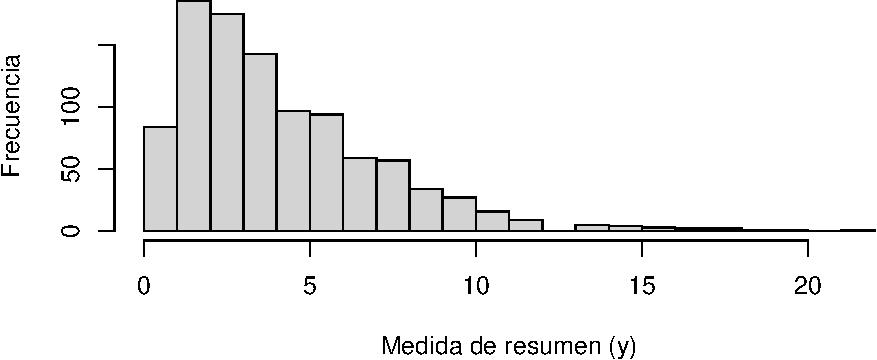
\includegraphics{05Estratificar_files/figure-latex/MedRes-1.pdf}
\caption{\label{fig:MedRes}\emph{Histograma de la medida de resumen (y) sobre las UPM}}
\end{figure}

\hypertarget{particiuxf3n-en-cuantiles-q}{%
\subsection{Partición en cuantiles (Q)}\label{particiuxf3n-en-cuantiles-q}}

Este método divide la población de UPM en grupos creados a partir de la división en intervalos regulares de la distribución de la medida de resumen. Los cuantiles más usados son los cuartiles (que dividen la población en cuatro grupos), los quintiles (que dividen la población en cinco grupos) y los deciles (que dividen la población en 10 grupos); sin embargo, con los propósitos de estratificación, también es útil considerar la partición en terciles (que dividen la población en tres grupos).

\hypertarget{muxe9todo-de-rauxedz-de-frecuencia-acumulada-dh}{%
\subsection{Método de raíz de frecuencia acumulada (DH)}\label{muxe9todo-de-rauxedz-de-frecuencia-acumulada-dh}}

\citet{Dalenius_Hodges_1959} propusieron esta técnica de estratificación basada en la raíz cuadrada de las frecuencias acumuladas de la medida de resumen sobre las UPM. Esta técnica es exacta y no requiere de algún procedimiento iterativo. La idea principal de esta técnica es encontrar grupos que minimicen la siguiente función:

\[
D = \sum_{h=1}^H W_h \sqrt{S^2_{y_{h}}}
\]

En donde \(W_h = N_h/N\) (\(h = 1, \ldots, H\)) es el tamaño relativo del estrato \(h\) y \(S^2_{y_{h}}\) es la varianza de la medida de resumen en el estrato \(h\).

\hypertarget{estratificaciuxf3n-uxf3ptima-lh}{%
\subsection{Estratificación óptima (LH)}\label{estratificaciuxf3n-uxf3ptima-lh}}

\citet{Lavallee_Hidiroglou_1988} propusieron por primera vez la construcción de una estratificación óptima para poblaciones de encuestas reales, basada en la minimización de la siguiente expresión ligada a la varianza de una estrategia de muestreo estratificada.

\[
\sum_{h=1}^{H-1} \left(\frac{N_h}{N}\right)^2\left(\frac{1}{(n-N_H)a_h}-\frac{1}{N_h}\right) S^2_{x_h}
\]

En donde \(N_h\) es el número de UPM en el estrato \(h\), \(n\) es el tamaño de muestra de las UPM, \(N\) es el número de UPM en el marco de muestreo, \(S^2_{x_h}\) es la varianza de la medida de resumen en el estrato \(h\). Finalmente \(a_h\) es la regla de asignación para el tamaño de muestra, dada por la siguiente relación:

\[
a_h = \frac{\gamma_h}{\sum_h \gamma_h}
\]

En donde, tomando en cuenta que \(\bar{X}_h\) es la media de la medida de resumen en el estrato \(h\), entonces, según \citep{Baillargeon_Rivest_2011}, \(\gamma_h\) es proporcional al tamaño de muestra \(n\) y está definida por:

\[
\gamma_h = N_h^{2q_1} \times  \bar{X}_h^{2q_2} \times S^{2q_3}_{x_h}
\]

Por tanto, dado que \(n_h = n \times \gamma_h\), si se quisiera una estrategia de muestreo que asigne el tamaño de muestra de manera proporcional a cada uno de los estratos, entonces la regla de asignación debería estar determinada por

\[
\mathbf q = (q_1, q_2, q_3)' = (0.5, 0, 0)'
\]

La asignación de Neyman corresponderá con \(\mathbf q = (0.5, 0, 0.5)'\); mientras que la asignación de potencia con exponente 0.7 estará dada por \(\mathbf q = (0.35, 0.35, 0)'\). Los detalles técnicos de estos tipos de asignación pueden ser encontrados en \citet{Gutierrez_2016}.

La optimización de la función objetivo puede ser llevada a cabo de diferentes formas. En efecto, \citet{Lavallee_Hidiroglou_1988} utilizaron un algoritmo de optimización (Sethi) para encontrar los valores óptimos. \citet{Baillargeon_Rivest_Ferland_2007} definen los pasos necesarios para implementar el procedimiento basado en el algoritmo de Sethi. Asimismo, \citet{Kozak_2004} definió un algoritmo iterativo mediante arranques aleatorios para optimizar el proceso de minimización de esta técnica de estratificación.

\hypertarget{estratificaciuxf3n-geomuxe9trica-gh}{%
\subsection{Estratificación geométrica (GH)}\label{estratificaciuxf3n-geomuxe9trica-gh}}

Utilizando las técnicas de estratificación mencionadas anteriormente, algunos autores se percataron de que, para poblaciones de UPM con medidas de resumen sesgadas, las varianzas relativas (coeficientes de variación) de la medida de resumen en cada estrato eran similares; es decir:

\[
\frac{S_{x_1}}{\bar{X}_1} \cong \frac{S_{x_2}}{\bar{X}_2} \cong \cdots \cong\frac{S_{x_H}}{\bar{X}_H}  
\]

\citet{Gunning_Horgan_2004} tomaron esta evidencia en consideración y desarrollaron este método con el objetivo de que los coeficientes de variación de la medida de resumen tiendan a ser iguales dentro de los estratos y, de esta forma, encontraron que los límites que definían estos grupos estaban conformados en progresión geométrica. Siendo \(X\) la variable que contiene la información de la medida de resumen para todas la UPM del marco de muestreo, entonces los límites de los estratos estarán dados por la siguiente expresión:

\[
b_h = \min(X) \left( \frac{\max X}{\min X} \right) ^ {h/L}; \ \ \ \ \ \ \ \ h = 1, 2, \ldots, H-1.
\]

Es posible encontrar que los coeficientes de variación de los estratos conformados por estos límites son equivalentes y por ende, este método es óptimo para encontrar mejores formas de estratificar teniendo en cuenta como función objetivo la variación relativa dentro los estratos.

\hypertarget{metodologuxedas-multivariadas-sobre-la-matriz-de-informaciuxf3n}{%
\section{Metodologías multivariadas sobre la matriz de información}\label{metodologuxedas-multivariadas-sobre-la-matriz-de-informaciuxf3n}}

Partiendo de la matriz de información \(\mathbf{X}\) a nivel de las UPM, la cual contiene \(N_I\) filas y \(P\) columnas, es posible considerar algunos procedimientos que no necesitan de la reducción a una sola dimensión, sino que admiten tantas dimensiones como indicadores definidos en las columnas de \(\mathbf{X}\). Teniendo en cuenta que en el periodo intercensal se realizarán encuestas que miden variables que están fuertemente ligadas a las observadas en el censo, entonces encontrar una estratificación que sea óptima para todo el conjunto de variables de la matriz de información asegurará una partición óptima para todas las encuestas realizadas en el periodo intercensal. Las siguientes metodologías permiten optimizar conjuntamente la eficiencia de la estratificación.

\hypertarget{k-medias-de-jarque-kmj}{%
\subsection{K-medias de Jarque (KmJ)}\label{k-medias-de-jarque-kmj}}

\citet{Jarque_1981} propuso utilizar una versión modificada del algoritmo de K-medias \citep{Macqueen_1967}, cuyo objetivo es la minimización de la siguiente función de distancia:

\[
\sum_{h=1}^H \sum_{k\in U_h}(\mathbf x_k - \bar {\mathbf x}_h)'\boldsymbol \Lambda^{-1}(\mathbf x_k - \bar {\mathbf x}_h)
\]

En donde \(\mathbf x_k\) corresponde a la medición de las \(P\) variables de la matriz de información en la \(k\)-ésima UPM, \(\bar {\mathbf x}_h\) es el vector de medias de la matriz de información en el estrato \(h\) y \(\boldsymbol \Lambda\) es una matriz diagonal de tamaño \(P \times P\) cuyas entradas se definen como la varianza de las \(P\) variables de la matriz \(\mathbf X\), es decir \(\boldsymbol \Lambda [p,p]=S^2_{x_p}\), con \(p = 1, 2, \ldots, P\). Esta modificación tiene como objetivo minimizar la relación entre la varianza de un estimador de muestreo estratificado con asignación proporcional y la de un muestreo aleatorio simple. Cuando \(\boldsymbol \Lambda = \mathbf I\), el algoritmo resultante es idéntico al algoritmo clásico de K-medias, propuesto por \citet{Macqueen_1967}.

\hypertarget{particiuxf3n-genuxe9tica-bb}{%
\subsection{Partición genética (BB)}\label{particiuxf3n-genuxe9tica-bb}}

\citet{Ballin_Barcaroli_2013} argumentan que la mejor estratificación es aquella partición del marco de muestreo que asegura el mínimo costo muestral que satisfaga algunas restricciones de precisión; o, que maximice la precisión de los indicadores de interés bajo las restricciones. De esta forma, el algoritmo busca minimizar la siguiente función de costos

\[
c_0 + \sum_{h=1}^{H} c_h n_h
\]

En donde \(c_0\) define un costo fijo y \(c_h\) es el costo promedio de observar un hogar en el estrato \(h\). En principio, es posible definir \(c_0=0\) y \(c_1 = c_2 = \cdots = c_H = 1\), lo cual da como resultado que el costo es el número de encuestas que deben realizarse en cada estrato. Este problema de optimización se complementa manteniendo las siguientes restricciones:

\[
\sum_{h=1}^{H} \left(\frac{N_h^2}{n_h}\right)\left(1-\frac{n_h}{N_h}\right) S^2_{x_h,p} \leq V_{0p}\ \ \  \ \ \ p = 1, 2, \ldots, P.
\]

En donde \(V_{0p}\) es un umbral predefinido por el usuario, que indica que la varianza de la estrategia estratificada está acotada; además, \(S^2_{x_h,p}\) es la varianza poblacional de \(p\)-ésima variable de la matriz de información en el estrato \(h\).
Haciendo uso de algoritmos genéticos evolutivos, esta estratificación multivariada del marco de muestreo parte de la consideración de estratificaciones univariadas independientes (una para cada variable de la matriz de información) y de la definición del producto cartesiano resultante de todas estas particiones (estratos atómicos). Este universo de posibles estratificaciones evoluciona, uniendo grupos de forma jerárquica, sujeto a las restricciones de precisión sobre cada variable de la matriz de información, hasta converger en el número de estratos definidos de antemano \(H\).

\hypertarget{evaluaciuxf3n-y-escogencia-de-la-mejor-estratificaciuxf3n}{%
\section{Evaluación y escogencia de la mejor estratificación}\label{evaluaciuxf3n-y-escogencia-de-la-mejor-estratificaciuxf3n}}

En la evaluación de los escenarios de estratificación entran las técnicas univariadas y multivariadas. Al final, el resultado de aplicar una u otra técnica es simplemente una clasificación de las UPM. Por lo tanto, cada una de las posibles estratificaciones debe ser evaluada con base en la reducción de la varianza para todos los indicadores considerados en la matriz de clasificación. La medida clásica con la que se juzgan las bondades de una estrategia de muestreo es el efecto de diseño (DEFF). Por lo tanto, la evaluación de la estratificación debe estar supeditada también a esta medida, que para la variable \(p = 1, \ldots, P\), está dada por:

\[
DEFF_p = \frac{Var_{ST}(\bar x _p)}{Var_{SI}(\bar x _p)} \ \ \ \ \ \ \ \ \ p = 1, \ldots, P.
\]

En donde, \(Var_{ST}(\bar x _p)\) y \(Var_{SI}(\bar x _p)\) denotan la varianza del diseño estratificado y la varianza de un muestreo aleatorio simple para la media poblacional (porcentaje) de la \(p\)-ésima variable de la matriz de información. Por otro lado, \citet[página 184]{Gutierrez_2016} demuestra que, cuando la asignación es proporcional, esta relación se puede escribir de la siguiente manera:

\[
DEFF_p = \frac{ \sum_{h=1}^H W_h S^2_{x_{hp}} }{S^2_{x_p}} \cong 1 - R^2_p \ \ \ \ \ \ \ \ \ p = 1, \ldots, P.
\]

En donde, para cada estrato \(h = 1, \ldots, H\), se tiene que \(S^2_{x_p}\) es la varianza de la variable \(x_p\) en la población y \(S^2_{x_{hp}}\) es la varianza de la variable \(x_p\) supeditada al estrato \(h\). Nótese que este efecto de diseño es función del coeficiente de determinación \(R^2_p\) en un modelo lineal con intercepto que relaciona la \(p\)-ésima variable de evaluación (respuesta) con los estratos (factores). Una ventaja de expresar el efecto de diseño como en la ecuación anterior es que no dependerá del tamaño de muestra. Una vez definido el criterio de evaluación de la estratificación sobre una variable \(x_p\), es necesario definir un criterio de estratificación multivariante que contemple cada una de las \(P\) variables. Siguiendo las ideas de \citet{Jarque_1981}, se propone la siguiente medida de calidad, definida como el \emph{efecto de diseño generalizado} (\(G(S)\)) sobre todas las variables de la matriz de información:

\[
G(S) = \sum_{p=1}^P DEFF_p = \sum_{p=1}^P \frac{1}{S^2_{x_p}}\sum_{h=1}^H W_h S^2_{x_{hp}}
\]

Ante una estratificación pertinente, se esperaría que \(Var_{ST}(\bar x _p) < Var_{SI}(\bar x _p)\), por lo tanto \(0 < DEFF_p < 1\), lo que conlleva a que \(0 < G(S) < P\). Luego, se debería escoger el escenario para el cual \(G(S)\) fuera mínimo. Nótese que, para cada uno de los escenarios en estudio, es necesario fijar el número de estratos; en general se propende a que el número de estratos esté entre tres y cinco. Esta escogencia del número de grupos debe ser discutida al interior del INE con los equipos que determinan la rotación de las UPM en cada periodo de levantamiento de las encuestas de hogares. Escoger un número alto de estratos reducirá la varianza, pero a su vez puede tener repercusiones negativas en la logística de rotación del diseño de muestreo de las encuestas, haciendo que se agoten rápidamente las UPM dentro de los estratos geográficos y socioeconómicos. Por lo anterior, se recomienda restringir los escenarios de evaluación a la consideración de \(H=3\) y \(H=4\) estratos.

El siguiente cuadro ejemplifica la evaluación de estas técnicas para dos escenarios de estratificación (tres y cuatro estratos) en una matriz de información que contiene 8 variables. De la tabla se puede deducir varias conclusiones interesantes. Por ejemplo, para el primer indicador, la mejor estratificación es la dada por el método de raíz de frecuencia acumulada (DH) con cuatro estratos; para el segundo indicador, la mejor estratificación es la partición genética (BB) con cuatro estratos; mientras que para el último indicador, la mejor estratificación es la estratificación óptima con el algoritmo de Sethi (LH) con cuatro estratos. Como se puede notar, para cada indicador existirá un método que induzca una mayor eficiencia que para otros indicadores. Esto claramente muestra que la estratificación con respecto a un solo indicador puede ser un procedimiento inadecuado. Por lo tanto, basados en este ejemplo, el mejor método sería el de Dalenious-Hidiroglou (DH) con cuatro estratos, puesto que induce una mayor eficiencia conjunta al reducir el efecto de diseño generalizado.

\footnotesize

\begin{longtable}[]{@{}
  >{\raggedleft\arraybackslash}p{(\columnwidth - 24\tabcolsep) * \real{0.0758}}
  >{\raggedleft\arraybackslash}p{(\columnwidth - 24\tabcolsep) * \real{0.0682}}
  >{\raggedleft\arraybackslash}p{(\columnwidth - 24\tabcolsep) * \real{0.0833}}
  >{\raggedleft\arraybackslash}p{(\columnwidth - 24\tabcolsep) * \real{0.0758}}
  >{\raggedleft\arraybackslash}p{(\columnwidth - 24\tabcolsep) * \real{0.0758}}
  >{\raggedleft\arraybackslash}p{(\columnwidth - 24\tabcolsep) * \real{0.0833}}
  >{\raggedleft\arraybackslash}p{(\columnwidth - 24\tabcolsep) * \real{0.0758}}
  >{\raggedleft\arraybackslash}p{(\columnwidth - 24\tabcolsep) * \real{0.0682}}
  >{\raggedleft\arraybackslash}p{(\columnwidth - 24\tabcolsep) * \real{0.0833}}
  >{\raggedleft\arraybackslash}p{(\columnwidth - 24\tabcolsep) * \real{0.0758}}
  >{\raggedleft\arraybackslash}p{(\columnwidth - 24\tabcolsep) * \real{0.0758}}
  >{\raggedleft\arraybackslash}p{(\columnwidth - 24\tabcolsep) * \real{0.0833}}
  >{\raggedleft\arraybackslash}p{(\columnwidth - 24\tabcolsep) * \real{0.0758}}@{}}
\caption{\emph{Efectos de diseño \(DEFF_p\) y efecto de diseño generalizado \(G(S)\) considerando tres (\(H=3\)) y cuatro (\(H=4\)) estratos para ocho variables.}}\tabularnewline
\toprule()
\begin{minipage}[b]{\linewidth}\raggedleft
DEFF
\end{minipage} & \begin{minipage}[b]{\linewidth}\raggedleft
Q (H=3)
\end{minipage} & \begin{minipage}[b]{\linewidth}\raggedleft
DH (H=3)
\end{minipage} & \begin{minipage}[b]{\linewidth}\raggedleft
LH (H=3)
\end{minipage} & \begin{minipage}[b]{\linewidth}\raggedleft
GH (H=3)
\end{minipage} & \begin{minipage}[b]{\linewidth}\raggedleft
KmJ (H=3)
\end{minipage} & \begin{minipage}[b]{\linewidth}\raggedleft
BB (H=3)
\end{minipage} & \begin{minipage}[b]{\linewidth}\raggedleft
Q (H=4)
\end{minipage} & \begin{minipage}[b]{\linewidth}\raggedleft
DH (H=4)
\end{minipage} & \begin{minipage}[b]{\linewidth}\raggedleft
LH (H=4)
\end{minipage} & \begin{minipage}[b]{\linewidth}\raggedleft
GH (H=4)
\end{minipage} & \begin{minipage}[b]{\linewidth}\raggedleft
KmJ (H=4)
\end{minipage} & \begin{minipage}[b]{\linewidth}\raggedleft
BB (H=4)
\end{minipage} \\
\midrule()
\endfirsthead
\toprule()
\begin{minipage}[b]{\linewidth}\raggedleft
DEFF
\end{minipage} & \begin{minipage}[b]{\linewidth}\raggedleft
Q (H=3)
\end{minipage} & \begin{minipage}[b]{\linewidth}\raggedleft
DH (H=3)
\end{minipage} & \begin{minipage}[b]{\linewidth}\raggedleft
LH (H=3)
\end{minipage} & \begin{minipage}[b]{\linewidth}\raggedleft
GH (H=3)
\end{minipage} & \begin{minipage}[b]{\linewidth}\raggedleft
KmJ (H=3)
\end{minipage} & \begin{minipage}[b]{\linewidth}\raggedleft
BB (H=3)
\end{minipage} & \begin{minipage}[b]{\linewidth}\raggedleft
Q (H=4)
\end{minipage} & \begin{minipage}[b]{\linewidth}\raggedleft
DH (H=4)
\end{minipage} & \begin{minipage}[b]{\linewidth}\raggedleft
LH (H=4)
\end{minipage} & \begin{minipage}[b]{\linewidth}\raggedleft
GH (H=4)
\end{minipage} & \begin{minipage}[b]{\linewidth}\raggedleft
KmJ (H=4)
\end{minipage} & \begin{minipage}[b]{\linewidth}\raggedleft
BB (H=4)
\end{minipage} \\
\midrule()
\endhead
\(\bar x_1\) & 0.87 & 0.85 & 0.81 & 0.82 & 1 & 0.88 & 0.8 & 0.70 & 0.76 & 0.72 & 0.71 & 0.77 \\
\(\bar x_2\) & 0.89 & 0.82 & 0.95 & 0.97 & 0.94 & 0.88 & 0.79 & 0.74 & 0.75 & 0.77 & 0.75 & 0.71 \\
\(\bar x_3\) & 0.87 & 0.97 & 0.83 & 0.96 & 0.89 & 0.95 & 0.74 & 0.75 & 0.79 & 0.7 & 0.79 & 0.71 \\
\(\bar x_4\) & 0.92 & 0.89 & 0.81 & 0.94 & 0.96 & 1 & 0.77 & 0.73 & 0.73 & 0.7 & 0.71 & 0.74 \\
\(\bar x_5\) & 0.85 & 0.83 & 0.96 & 0.96 & 0.83 & 0.81 & 0.8 & 0.73 & 0.8 & 0.78 & 0.8 & 0.79 \\
\(\bar x_6\) & 0.87 & 0.88 & 0.9 & 0.88 & 0.86 & 0.81 & 0.8 & 0.72 & 0.76 & 0.7 & 0.74 & 0.73 \\
\(\bar x_7\) & 0.87 & 0.95 & 0.99 & 0.83 & 0.86 & 0.84 & 0.75 & 0.7 & 0.77 & 0.72 & 0.77 & 0.77 \\
\(\bar x_8\) & 0.93 & 0.82 & 0.91 & 0.99 & 0.93 & 0.88 & 0.77 & 0.74 & 0.72 & 0.78 & 0.76 & 0.75 \\
G(S) & 7.07 & 7.01 & 7.16 & 7.35 & 7.27 & 7.05 & 6.22 & 5.81 & 6.08 & 5.87 & 6.03 & 5.97 \\
\bottomrule()
\end{longtable}

\normalsize

Para estudiar la comparabilidad y consistencia del proceso de estratificación, los algoritmos de evaluación se deberían aplicar sobre cada una de las UPM en las áreas urbanas, pero independientemente de las UPM rurales.Si la ganancia en eficiencia es mayor en este escenario, se pueden definir los estratos de forma independiente. Si, por el contrario, la comparabilidad entre estratos es imperante en el proceso de estratificación, se puede considerar únicamente el escenario conjunto en donde las UPM de la zona urbana y rural están presentes conjuntamente. En este último caso, la clasificación de las UPM de la zona urbana se regirá por las mimas condiciones que sus contrapartes urbanas.

Al margen de la técnica utilizada para encontrar la mejor clasificación de las UPM, se recalca que la viabilidad sobre el número de estratos sea discutida de forma exhaustiva por todas las áreas involucradas al interior de los INE. En forma general, es recomendable restringir los escenarios de evaluación a la consideración de H=3 o H=4 estratos. Este último componente es importante puesto que los diseños de muestreo deberían considerar un tamaño de muestra mínimo de dos UPM por estrato para poder estimar la varianza del estimador \citep{Gutierrez_2016}.

El efecto diseño no es el único aspecto por evaluar para la elección del procedimiento de estratificación. Es necesario verificar la estabilidad del método con respecto a los otros procedimientos de estratificación. Por ejemplo, la siguiente tabla muestra la matriz de coincidencias entre las diferentes clasificaciones de los estratos.

\begin{longtable}[]{@{}
  >{\centering\arraybackslash}p{(\columnwidth - 14\tabcolsep) * \real{0.1646}}
  >{\centering\arraybackslash}p{(\columnwidth - 14\tabcolsep) * \real{0.1266}}
  >{\centering\arraybackslash}p{(\columnwidth - 14\tabcolsep) * \real{0.1392}}
  >{\centering\arraybackslash}p{(\columnwidth - 14\tabcolsep) * \real{0.1013}}
  >{\centering\arraybackslash}p{(\columnwidth - 14\tabcolsep) * \real{0.1013}}
  >{\centering\arraybackslash}p{(\columnwidth - 14\tabcolsep) * \real{0.1013}}
  >{\centering\arraybackslash}p{(\columnwidth - 14\tabcolsep) * \real{0.1013}}
  >{\centering\arraybackslash}p{(\columnwidth - 14\tabcolsep) * \real{0.1646}}@{}}
\caption{\emph{Matriz de coincidencias, cuyas entradas están definidas como el porcentaje de UPM coincidentes en cada uno de los estratos creados por los métodos estudiados.}}\tabularnewline
\toprule()
\begin{minipage}[b]{\linewidth}\centering
Técnica
\end{minipage} & \begin{minipage}[b]{\linewidth}\centering
Jarque
\end{minipage} & \begin{minipage}[b]{\linewidth}\centering
K-means
\end{minipage} & \begin{minipage}[b]{\linewidth}\centering
DAL
\end{minipage} & \begin{minipage}[b]{\linewidth}\centering
GEO
\end{minipage} & \begin{minipage}[b]{\linewidth}\centering
LH-S
\end{minipage} & \begin{minipage}[b]{\linewidth}\centering
LH-K
\end{minipage} & \begin{minipage}[b]{\linewidth}\centering
Percentil
\end{minipage} \\
\midrule()
\endfirsthead
\toprule()
\begin{minipage}[b]{\linewidth}\centering
Técnica
\end{minipage} & \begin{minipage}[b]{\linewidth}\centering
Jarque
\end{minipage} & \begin{minipage}[b]{\linewidth}\centering
K-means
\end{minipage} & \begin{minipage}[b]{\linewidth}\centering
DAL
\end{minipage} & \begin{minipage}[b]{\linewidth}\centering
GEO
\end{minipage} & \begin{minipage}[b]{\linewidth}\centering
LH-S
\end{minipage} & \begin{minipage}[b]{\linewidth}\centering
LH-K
\end{minipage} & \begin{minipage}[b]{\linewidth}\centering
Percentil
\end{minipage} \\
\midrule()
\endhead
\textbf{Q} & 1 & 0,64 & 0,92 & 0,84 & 0,89 & 0,89 & 0,82 \\
\textbf{DH} & 0,64 & 1 & 0,68 & 0,62 & 0,71 & 0,71 & 0,74 \\
\textbf{LH} & 0,92 & 0,68 & 1 & 0,82 & 0,96 & 0,96 & 0,90 \\
\textbf{GH} & 0,84 & 0,62 & 0,82 & 1 & 0,78 & 0,78 & 0,73 \\
\textbf{KmJ} & 0,89 & 0,71 & 0,96 & 0,78 & 1 & 1,00 & 0,93 \\
\textbf{BB} & 0,89 & 0,71 & 0,96 & 0,78 & 1,00 & 1 & 0,93 \\
\bottomrule()
\end{longtable}

Por último, también se debe evaluar la coherencia de la distribución de las diferentes variables agregadas a nivel de UPM en los estratos. Por ejemplo, la proporción de personas mayores de 15 años alfabetizadas debería tener mayor incidencia en los estratos más altos, y este patrón también se debería observar para diferentes indicadores como la proporción de hogares con internet, la proporción de tenencia de refrigerador, la proporción de tenencia de televisión por cable, la proporción de tenencia de automóvil, la proporción de hogares con saneamiento adecuado, la proporción de hogares con pisos adecuados, la proporción de personas con educación superior, entre otras. La figura \ref{fig:estrata} muestra el comportamiento esperado en los estratos de muestreo para algunas variables de interés. De esta forma, el estrato uno debería presentar condiciones económicas más adversas, el estrato dos debería tener mejores condiciones, siendo el tercer estrato el que agrupa a las UPM con menores dificultades socioeconómicas. En el área rural debiesen aparecer una menor proporción de UPM en el estrato 3, dadas las condiciones menos favorables.

\begin{figure}
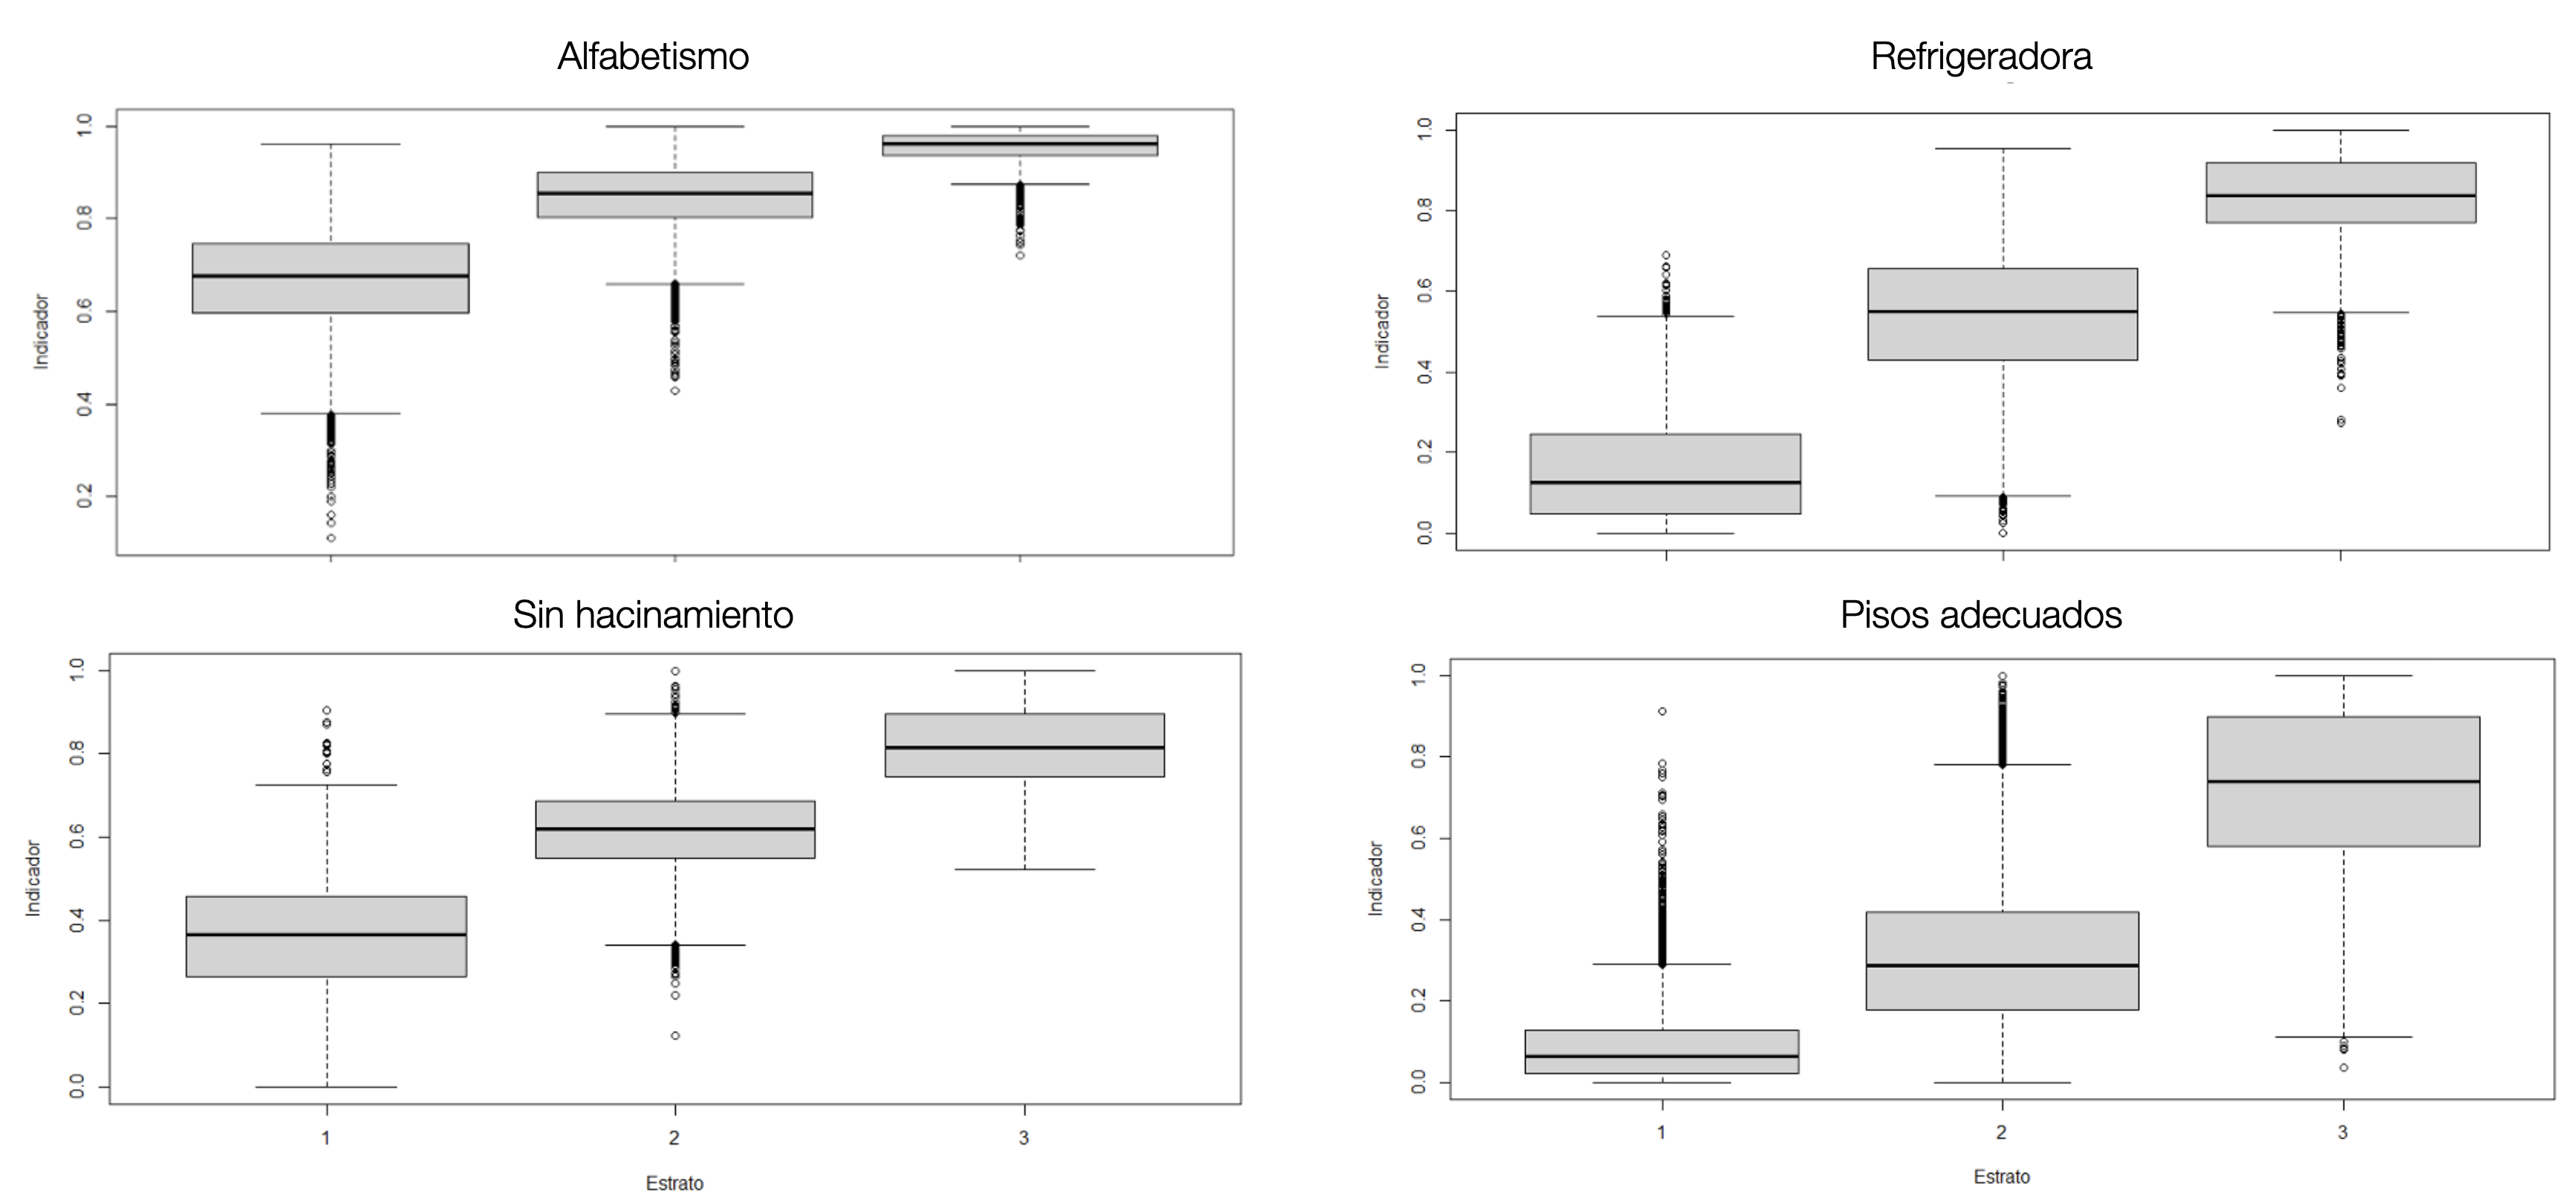
\includegraphics[width=800px]{Pics/Estratificar} \caption{Comportamiento esperado en los estratos de muestreo para algunas variables de interés.}\label{fig:estrata}
\end{figure}

Si la contribución de algunas unidades al total poblacional es no significativa, y además esas unidades son de difícil acceso, es común que en algunos países de la región se opte por redefinir el universo y crear un estrato de exclusión forzosa. En este estrato no se realiza ninguna encuesta y las respectivas estimaciones no tendrán en cuenta a esta población excluida. Por último, como algunos procedimientos de clasificación se basan en la generación de números aleatorios, se recomienda documentar los códigos computacionales que se utilizaron para que los resultados puedan ser replicados, por lo que debe fijar una semilla aleatoria al comienzo del código computacional.

\hypertarget{estratificaciuxf3n-impluxedcita}{%
\section{Estratificación implícita}\label{estratificaciuxf3n-impluxedcita}}

Los estratos explícitos definidos en la sección anterior son útiles para reducir la varianza de muestreo y asegurar la representatividad de la muestra en cada uno de los subgrupos que comparten las mismas características socioeconómicas, dentro de los mismos municipios. Además de los estratos socioeconómicos, algunas variables que se consideran en el proceso de estratificación explícita son:

\begin{itemize}
\tightlist
\item
  Estados o regiones de un país.
\item
  Zona en la que está ubicado el hogar: urbana o rural. Nótese que cada país brinda su definición de ruralidad, de acuerdo con sus propias definiciones nacionales.
\end{itemize}

También es posible realizar una selección ordenada que induce una estratificación implícita, sin que necesariamente se tenga control sobre el tamaño de muestra final, y sin asumir independencia en la selección. Este tipo de estratificación es una forma de garantizar una asignación estrictamente proporcional de los hogares en todos los estratos implícitos. También puede conducir a una mayor confiabilidad de las estimaciones de la encuesta, siempre que las variables de estratificación implícita que se consideren estén correlacionadas con los indicadores de interés (por ejemplo, la tasa de desocupación, subocpupación o informalidad).

La estratificación implícita es altamente recomendada cuando la encuesta está enfocada en un tema particular (como por ejemplo el mercado de trabajo) y requiere el uso del muestreo sistemático (con probabilidades simples o desiguales) en la selección de las UPM. Según \citet[pág. 46]{UN_2008}, en la mayoría de países la secuencia podría empezar con el área urbana, desagregada por departamento, a su vez desagregada por municipio; seguida del área rural, desagregada por departamento, a su vez desagregada por comuna o vereda. La selección sistemática de UPM deberá estar supeditada al ordenamiento de las UPM por el número de viviendas.

Nótese que la estratificación implícita puede constituir un método objetivo de selección de reemplazos de las UPM a las cuales no se pudo acceder en el operativo de campo; de esta forma, si una UPM fue seleccionada originalmente, pero por alguna razón operativa no puede ser empadronada, su reemplazo será la inmediatamente anterior (o posterior) en la lista estratificada implícitamente. Nótese que este procedimiento ubicará el reemplazo como la UPM ubicada en el mismo municipio, dentro del mismo departamento, en la misma zona y con un número similar de viviendas.

Aunque la estratificación implícita permite acotar el sesgo generado por la ausencia de respuesta de las UPM, \citet[págs. 348 - 349]{Vehovar_1999} advierte que se debe tener precaución en cuanto a los usos de esta práctica puesto que puede conllevar sesgos importantes en las estimaciones de interés. Lo anterior se desprende del hecho de que los individuos ubicados en zonas donde sí es posible acceder puedan diferir significativamente de aquellos ubicados en las zonas de difícil acceso, las cuales difícilmente serán seleccionadas por los algoritmos de muestreo que hacen uso de la estratificación implícita.

Por esta razón es útil que, después de haber valorado los posibles sesgos, si se ha tomado la determinación de realizar las sustituciones sobre las UPM de difícil acceso, se realice un seguimiento exhaustivo en cada levantamiento que permita clasificar el esquema de recolección de información primaria y se valore su impacto en la precisión de los estimadores resultantes.

\hypertarget{diseuxf1o-y-mecanismo-de-selecciuxf3n-de-la-muestra}{%
\chapter{Diseño y mecanismo de selección de la muestra}\label{diseuxf1o-y-mecanismo-de-selecciuxf3n-de-la-muestra}}

Todas las encuestas de hogares en la región comparten el mismo principio inferencial: la selección de una muestra que puede representar la población de todo un país. Por supuesto, ante este objetivo tan ambicioso, es necesario contar con procedimientos robustos, probados y capaces de pasar los filtros más críticos y agudos. Tal vez en este momento de la historia, la práctica de estos procedimientos ya no genere ningún tipo de asombro, pero el lector podría animarse a contemplar todos los posibles escenarios que una sociedad enfrentaría ante la ausencia de las encuestas de hogares y sus repercusiones en materia de seguimiento del desarrollo social y económico.

Es innegable la potencia y el poder que hay detrás de estas operaciones estadísticas que están sustentadas en el muestreo probabilístico que induce una inferencia que procede de lo particular a lo general, puesto que al seleccionar una muestra, esta sirve como base para obtener conclusiones acerca de la población. Al final la muestra será un vehículo adecuado para representar las características más importantes de la población en estudio, en la forma en que justamente las variables se incorporan en el formulario de la encuesta. \citet{Gutierrez_2016} afirma que el muestreo es un procedimiento que responde a la necesidad de información estadística precisa sobre la población y los conjuntos de elementos que la conforman; asimismo comenta que el muestreo probabilístico trata con investigaciones parciales que apuntan a inferir a la población completa y en general está basado en los siguientes principios:

\begin{itemize}
\tightlist
\item
  \emph{Aleatorización}: las unidades incluidas en la muestra son seleccionadas mediante un proceso probabilístico. De esta forma, además de eliminar los posibles sesgos de selección, la muestra resultante será válida para cualquier proceso de inferencia, puesto que se basa en el conjunto de todas las muestras que se pueden obtener con el esquema de muestreo definido.
\item
  \emph{Inclusión}: todas las unidades de la población tienen una probabilidad no nula de ser incluidas en la muestra. Lo anterior quiere decir que el procedimiento de selección le da chance de ser seleccionado a todas las unidades que componen la población. De esta manera, la muestra final puede estar compuesta por cualquier combinación plausible de hogares o individuos.
  Para que los anteriores principios se cumplan a cabalidad, es necesario contar con un instrumento que permita seleccionar a los hogares del país de forma exhaustiva y completa; esto quiere decir que el instrumento debería contener todos y cada uno de los hogares de la población. Dado que no existe una lista que permita identificar y ubicar a cada uno de los hogares de la población, entonces se deben contemplar otras posibilidades que permitan lograr el objetivo. Debido al principio natural de la aglomeración de las poblaciones humanas, es posible lograr este cometido de manera indirecta a través de la definición de los marcos de muestreo de áreas.
\end{itemize}

Las encuestas han tenido una gran trascendencia en la evolución de las mediciones de los indicadores sociales, que a su vez conllevan a que los gobiernos realicen un seguimiento y monitoreo de las cifras más importantes para la sociedad. De esta forma se podrá investigar la efectividad de las políticas públicas, para concretar las metas de mejora en las condiciones sociales y/o económicas de la ciudadanía. Tal como lo afirma \citet{Gutierrez_2016}, el muestreo es un procedimiento que responde a la necesidad de información estadística precisa sobre la población y los conjuntos de elementos que la conforman. De esta forma, una muestra bien seleccionada de unos cuantos miles de individuos puede representar con gran precisión a una población de millones de personas.

En general, se puede afirmar que un concepto apropiado por la sociedad es el que define a una muestra representativa como un modelo reducido de la población. De este concepto se desprende un argumento de validez sobre la muestra: ``una buena muestra es aquella que se parece a la población, de tal forma que las categorías aparecen con las mismas proporciones que en la población''. Sin embargo, en algunos casos es fundamental ``sobrerepresentar'' algunas categorías o incluso seleccionar unidades con probabilidades desiguales \citep{Tille2006}. La muestra no debe ser un modelo reducido de la población; debe ser una herramienta usada para obtener estimaciones válidas: exactas, confiables, precisas y consistentes.

El concepto de muestra representativa no se debe usar para referirse a que la muestra debe parecerse a la población. La teoría de muestreo se ha ocupado de estudiar estrategias óptimas que permitan asegurar la calidad de las estimaciones; en general, el concepto de representatividad debe estar asociado con la estrategia de muestreo y no sólo con la muestra seleccionada. Consecuentemente, es la muestra expandida la que debe recibir el calificativo de representativa, puesto que su objetivo es reflejar a la población y permitir que, mediante la correcta caracterización de una estrategia de muestreo, el proceso de inferencia logre reproducir sus estructuras.

El objetivo del equipo técnico experto en la selección de muestras debe estar supeditado a lograr que efectivamente este adjetivo (representatividad) se pueda aplicar a todo el componente de diseño y estimación. Es decir, el calificativo de representatividad es objeto de un proceso conjunto de diseño de muestreo, estimación de parámetros, acercamiento a modelos estadísticos para hacer frente a la ausencia de respuesta, entre otros. Uno de los objetivos de este capítulo será hacer precisión sobre las estructuras de selección de las muestras en las encuestas por muestreo. Al escoger un mecanismo apropiado para la selección de la muestra, será posible afirmar que la estrategia de muestreo es efectivamente representativa de la población de interés, puesto que cumple con altos estándares de rigurosidad y calidad en cada uno de los componentes del proceso.

\hypertarget{diseuxf1os-de-muestreo}{%
\section{Diseños de muestreo}\label{diseuxf1os-de-muestreo}}

Una vez que los marcos de muestreo se han refinado y se ha definido una estratificación apropiada para las UPM que las componen, es necesario realizar el proceso de muestreo para la selección final de los hogares. Este proceso de selección debe inducir insesgamiento, además de ser eficiente. Esto quiere decir que la inclusión de las unidades en la muestra estará supeditada a un esquema probabilístico libre de cualquier sesgo. Además de esto, se necesita que este mecanismo genere la menor dispersión posible en el proceso inferencial posterior.

El procedimiento de muestreo le asigna una probabilidad de selección conocida a cada posible muestra. Al diseñar un muestreo probabilístico, el investigador es el encargado de asignar estas probabilidades, mediante la definición del diseño de muestreo \citep{Sarndal_Swensson_Wretman_2003}. Aunque esta asignación de probabilidades se realiza de manera teórica, la pericia del equipo técnico deberá establecer cuál es la mejor forma de selección, y sobre esta escoger el mejor algoritmo de muestreo. Luego de establecer este conjunto de probabilidades, una única muestra es escogida mediante un mecanismo aleatorio que siga a cabalidad esta configuración estocástica inducida por el diseño de muestreo. Las probabilidades deben ser distintas de cero puesto que, de lo contrario, no se podría garantizar una inferencia insesgada, puesto que estaría excluyendo algunos sectores cartográficos del país. Además, estas mismas probabilidades se utilizan para crear los factores de expansión que definen todo el proceso de estimación, junto con el cálculo de los errores de muestreo, como se verá en los capítulos posteriores.

Existe una clara diferenciación entre un diseño de muestreo y un algoritmo de muestreo. El primero indica qué probabilidad de selección tendrán las posibles muestras en el soporte de muestreo, definido como el conjunto de todas las posibles muestras. Y el último se define como el proceso de selección de una única muestra que respeta las probabilidades del diseño de muestreo. En la definición de una encuesta de hogares es indispensable que se establezcan de antemano estos dos componentes. Es decir, si se ha decidido que el diseño de muestreo sea en etapas, el equipo técnico deberá documentar exhaustivamente cada etapa de muestreo, definiendo sus correspondientes unidades de muestreo y por consiguiente, los diseños de muestreos en cada etapa. Luego, es igual de importante explicar qué algoritmos de selección serán utilizados en cada etapa de muestreo. De esta forma habrá total transparencia en la selección de las unidades y esto redunda en la obtención de cifras oficiales confiables y precisas.

Existen muchas formas de seleccionar una muestra de hogares y cada una de ellas induce una medida de probabilidad sobre los elementos que conforman la población de interés. En general, asociado a cada esquema particular de muestreo se define una única función que asocia a cada hogar \(k\) con una probabilidad de inclusión en la muestra \(s\), definida de la siguiente manera:

\[\pi_k = Pr (k \in s)\]

Si el diseño de muestreo es de tamaño fijo, estas probabilidades de inclusión de los hogares cumplirán con las siguientes propiedades

\begin{enumerate}
\def\labelenumi{\arabic{enumi}.}
\tightlist
\item
  \(\pi_k > 0\)
\item
  \(\sum_U \pi_k = n\)
\end{enumerate}

Observe que la primera propiedad garantiza que ningún hogar será excluido de la selección inicial. Si bien no todos los hogares serán seleccionados para pertenecer a la muestra \(s\), todos tendrán un chance de ser escogidos por el mecanismo de selección aleatorio. En segunda medida, el tamaño de la muestra de hogares estará inducido por la magnitud de las probabilidades de inclusión. Por esta razón, una encuesta con una tamaño de muestra grande asignará una mayor probabilidad de inclusión a todos los hogares, que una encuesta de tamaño de muestra más modesto. A continuación se presenta una lista no exhaustiva de diseños de muestreo utilizados en encuestas de hogares para la publicación de estadísticas oficiales, junto con la forma particular que toman las probabilidades de inclusión en cada esquema.

\hypertarget{muestreo-aleatorio-simple}{%
\subsection{Muestreo aleatorio simple}\label{muestreo-aleatorio-simple}}

Este diseño de muestreo supone que es posible realizar una enumeración de todas las posibles muestras de tamaño fijo y escoger una de ellas mediante una selección aleatoria que asigne la misma probabilidad a cada una. Para ejecutar este diseño de muestreo es necesario tener información suficiente y exhaustiva de la ubicación e identificación de todas las unidades de interés. Su uso es común en las etapas finales de selección de las encuestas, en donde los hogares o personas se seleccionan con las misma probabilidad. Por ejemplo, una vez se ha escogido una UPM, una parte del operativo de campo deberá estar dedicada al enlistamiento de todas las viviendas y estructuras pertencientes a la UPM. Cuando se haya realizado este empadronamiento será posible asignarle la misma probabilidad de inclusión a cada vivienda en la UPM. Por ende, las probabilidades de inclusión en el muestreo aleatorio simple sin reemplazo son todas iguales y están dadas por la siguiente expresión:

\[\pi_k = Pr(k \in s) =  \frac{\binom{1}{1}\binom{N-1}{n-1}}{\binom{N}{k}} = \frac{n}{N}\]

Como se verá en los siguientes capítulos, cuando se usa el estimador de Horvitz-Thompson en este diseño de muestreo para estimar un total poblacional, y suponiendo que \(S^2_{y_U}\) denota la varianza de la característica de interés en la población finita, entonces las expresiones del estimador puntual y su varianza, respectivamente, toman la siguiente forma:

\begin{align*}
\hat{t}_{y,\pi} &= \sum_{s} \frac{y_k}{\pi_k} \\
Var(\hat{t}_{y,\pi}) &= \frac{N^2}{n}\left(1-\frac{n}{N}\right)S^2_{y_U}
\end{align*}

Una variante de este tipo de esquemas de selección de muestras de hogares dentro de la UPM es el muestreo sistemático, en donde se ordena el marco con algún patrón predefinido y posteriormente se selecciona un primer hogar (como arranque aleatorio). A partir de ese primer hogar seleccionado, se incluyen los restantes hogares en la muestra mediante saltos sistemáticos equi-espaciados por el siguiente factor \(a = \left \lfloor{N/n}\right \rfloor\), conocido como el intervalo de salto. Por ejemplo, una muestra sistemática podría ser:
\[s=\{2, 12, 22, 32, 42\}.\]

En donde el primer hogar elegido en la UPM fue el segundo y con saltos sistemáticos de diez hogares se va encuestando los restantes hogares en la lista. En este diseño la probabilidad de inclusión también es uniforme para cada hogar en la UPM y está dada por la siguiente expresión
\[\pi_k = Pr(k \in s) = \frac{1}{a} \approx \frac{n}{N}\]

\hypertarget{muestreo-proporcional-al-tamauxf1o}{%
\subsection{Muestreo proporcional al tamaño}\label{muestreo-proporcional-al-tamauxf1o}}

Este tipo de muestreo utiliza como insumo una característica de información auxiliar cuantitativa, también conocida como medida de tamaño (en inglés conocida como \emph{measure of size}). Para la ejecución de este diseño, necesariamente el marco de muestreo deberá contener el valor correspondiente a la medida de tamaño para cada una de sus unidades. Este muestreo es utilizado con frecuencia en las etapas iniciales de selección de las muestras, particularmente en la selección de las UPM que harán parte de la muestra. De esta forma, los conglomerados o UPM con más hogares o personas (medida de tamaño) tendrán una mayor probabilidad de ser seleccionados en la muestra. Por consiguiente, las probabilidades de inclusión en la muestra para las UPM serán desiguales y proporcionales a la medida de tamaño. Observe que la cantidad de individuos en las UPM es una cifra conocida, puesto que son resultado directo de los censos de población y vivienda.

Una de las ventajas de este tipo de muestreos es que hace más eficiente la estimación de los indicadores de interés. Para que esto ocurra, la medida de tamaño debe estar linealmente relacionada con la característica de interés. Esto a menudo sucede en las problemáticas sociales indagadas en las encuestas de hogares; puesto que a mayor número de hogares, se observa una mayor incidencia de estos fenómenos. Por ejemplo, restringidos a un estrato particular, es evidente que en las UPM con mas hogares se observarán mayor número de personas pobres, o de hogares con ingresos bajos, o de personas desocupadas, etc.

Por último, la medida de tamaño no necesariamente tiene que estar definida como el conteo simple de hogares o personas dentro de las UPM, también puede definirse como una función de estos conteos; por ejemplo, la raíz cuadrada, o incluso como una función compuesta de conteos de subpoblaciones. En el caso más simple, si \(N_i\) es la medida de tamaño de la \(i\)-ésima UPM \(U_i\), es decir el número de hogares que componen esa UPM; \(n_I\) el número de UPM que serán seleccionadas en cada estrato y \(N\) la sumatoria (o total) del número de hogares en todas las UPM del estrato (es decir, el número de hogares en el estrato) se tiene que las probabilidades de inclusión a la muestra \(s_I\) están dadas por la siguiente expresión:

\[\pi_i = Pr(U_i \in s_I) = n_I * \frac{N_i}{N}\]

\hypertarget{muestreo-estratificado}{%
\subsection{Muestreo estratificado}\label{muestreo-estratificado}}

Esta familia de diseños de muestreo permite realizar inferencias precisas en subgrupos poblacionales de interés, usualmente definidos como agregaciones geográficas grandes. Por ejemplo, si se quieren estimaciones de la incidencia de la pobreza en las regiones geográficas de un país específico, entonces es pertinente que esta división geográfica sea considerada para la definición de los estratos. Como se mencionó al inicio de este capítulo, estas divisiones territoriales se forman de manera natural, puesto que los estratos ya están definidos como regiones de interés en el seguimiento de los indicadores sociales. Por supuesto, es posible que la estrategia de muestreo cambie dependiendo de los estratos. Por ejemplo, en la planificación de las encuestas de uso de tiempo, una de las características de interés por las cuales se quiere indagar es la cantidad de horas que hombres y mujeres dedican a actividades de trabajo no remuneradas. Esta realidad cambia radicalmente entre zonas rurales y urbanas. Para este tipo de encuestas de hogares, la flexibilidad que tienen los diseños estratificados es un baluarte valioso que permite definir estrategias de muestreo más precisas.

Una consecuencia directa de la estratificación es que cada subgrupo tendrá un marco de muestreo de UPM independiente y mutuamente excluyente. Esta última caracterización induce una de las mayores ventajas del muestreo estratificado puesto que hay independencia entre los estratos. Esto significa que, al interior de cada estrato, se pueden ejecutar distintas estrategias de muestreo de forma independiente. Es común que en los países de América Latina el cruce de las áreas geográficas grandes junto con la división socioeconómica conformen los estratos (justo como se ilustró en los capítulos anteriores); asimismo una desagregación común en investigación social es la división territorial del país: urbano y rural. Evidentemente, la realidad social del entorno urbano difiere tanto del entorno rural que bien vale la pena considerar esta escisión en el diseño de muestreo de las encuestas de hogares.

Las probabilidades de inclusión definidas por este diseño de muestreo variarán en función de cada estrato \(h\) (\(h=1, \ldots, H\)). Por ejemplo, si se hubiese planeado un diseño aleatorio simple en cada estrato, entonces las probabilidades de inclusión estarían dadas por la siguiente expresión

\[\pi_k = Pr(k \in s_h) = \frac{n_h}{N_h}\]

En donde \(s_h\) define la muestra seleccionada en el estrato \(h\), \(N_h\) sería el número de hogares en ese estrato y \(n_h\) el tamaño de la muestra de hogares asociado a ese estrato.

En algunas ocasiones, se ha sugerido que el muestreo estratificado es el mejor diseño para una encuesta de hogares, lo cual es parcialmente cierto. Aunque en muchas ocasiones, la opción de estratificar es adecuada e inclusive conveniente, no es cierto estrictamente que el muestreo estratificado sea el mejor diseño de muestreo. De hecho, la varianza inducida por el diseño aleatorio estratificado puede llegar a ser más grande cuando no hay una clara homogeneidad en el comportamiento de la característica de interés dentro de los estratos.

\hypertarget{muestreo-de-conglomerados}{%
\subsection{Muestreo de conglomerados}\label{muestreo-de-conglomerados}}

Este diseño de muestreo surge como contraparte a la imposibilidad de generar una muestra de hogares directamente de un marco de muestreo que enliste todos y cada uno de los hogares en un país. De hecho, de forma hipotética, si fuese posible, los costos generados por una muestra aleatoria simple serían tan altos que la harían inviable desde el punto de vista presupuestario. Así, ante la ausencia de un marco de muestreo de las unidades de interés, y aprovechando el principio de aglomeración de las poblaciones humanas (que forman hogares y se aglomeran en segmentos, ciudades, regiones, etc.), la idea general detrás de este diseño es la conformación de unidades homogéneas entre sí (conglomerados), de las cuales se extraerá una muestra y para cada elemento del conglomerado se realizará un proceso exhaustivo de medición censal. De esta forma, es natural definir a las UPM como los conglomerados. Luego de seleccionar una muestra de estas UPM se realiza un censo de hogares dentro de cada una de las UPM seleccionadas. Nótese que este proceso logístico induce un esquema con ventajas económicas en términos presupuestales, puesto que limita el operativo de campo a un cierto número de UPM que se deben medir exhaustivamente.

A pesar de que esta estrategia resulte conveniente desde el punto de vista logístico y operativo, ciertamente no lo es desde el punto de vista de la eficiencia estadística; los errores de muestreo que se producen al utilizar esta metodología son bastante más elevados que en un diseño simple, puesto que al realizar el proceso de aglomeración, generalmente la variación interna de los conglomerados es muy baja y la variación entre conglomerados tiende a ser muy alta, generando mayor incertidumbre en la inferencia de la encuesta. Para superar estos inconvenientes, se podría pensar en un esquema de muestreo que aumente el tamaño de la muestra de conglomerados; sin embargo, este aumento puede llegar a ser tan grande que, en algunos estratos, se deberían seleccionar todas las UPM. Por supuesto, se trata de un esquema inviable en la práctica, pero que da paso al esquema de muestreo más común en las encuestas de hogares: la selección por etapas.

\hypertarget{muestreo-en-varias-etapas}{%
\subsection{Muestreo en varias etapas}\label{muestreo-en-varias-etapas}}

En este esquema de muestreo, la idea general es retomar los principios del muestreo de conglomerados y realizar un submuestreo de hogares dentro de los conglomerados o UPM seleccionadas inicialmente. En general, en América Latina son muy comunes los esquemas de selección en dos etapas: en la primera etapa se selecciona una muestra de UPM y en la segunda etapa se selecciona una muestra de hogares en aquellas UPM seleccionadas en la primera etapa. Aunque, también es posible encontrar en algunos países esquemas en más de dos etapas. Por ejemplo, en una primera etapa se seleccionan municipios; en una segunda etapa se seleccionan UPM dentro de los municipios seleccionados; y en la tercera se selecciona una muestra de hogares en aquellas UPM seleccionadas en la segunda etapa pertenecientes a los muniicpios seleccionados en la primera etapa de muestreo. Si un municipio es incluido en la muestra es posible realizar un proceso jerárquico y sistemático, hasta llegar a la unidad de observación. Por ejemplo, en una ciudad seleccionada, es posible hacer un submuestreo de sus secciones cartográficas, luego seleccionar sectores cartográficos (contenidos en las secciones) y por último seleccionar hogares o personas.

Si el esquema de muestreo incluye la selección de municipios en la primera etapa, el diseño de muestreo apropiado en esta instancia deberá ser proporcional a una medida de tamaño, que puede ser definida como el número de habitantes de los municipios. De esta forma, con una probabilidad muy grande, a veces igual a uno, las ciudades más importantes (con más habitantes) serán siempre parte del estudio. Por otro lado, es posible que en algunas encuestas exista un submuetreo de personas dentro del hogar. En este caso, \citet{Clark_Steel_2007} aclaran que la escogencia de las personas dentro de los hogares no debería ser aleatoria simple puesto que ciertos grupos poblacionales podrían estar sub-representados o sobre-presentados. En general, el muestreo en varias etapas tiene dos características esenciales que lo hacen robusto, en términos estadísticos, y eficiente al momento de planear la logística del levantamiento de información; estas son:

\begin{itemize}
\tightlist
\item
  La independencia: que implica que no hay ninguna correlación en el diseño de muestreo de las unidades primarias de muestreo. Esto quiere decir que en cada UPM se puede ejecutar con independencia cualquier estrategia de muestreo que se crea apropiada para seleccionar la submuestra de hogares.
\item
  La invarianza: que implica que sin importar qué diseño de muestreo se ejecutó en la primera etapa para seleccionar las UPM, la segunda etapa de selección podrá ejecutarse de manera independiente de la primera etapa. Es decir, el submuestreo de los hogares es independiente del muestreo de las UPM.
\end{itemize}

Un esquema de selección bastante usado en las encuestas de hogares de América Latina es el relacionado con los diseños auto-ponderados, lo cuales, en la primera etapa de muestreo se seleccionan \(n_I\) de \(N_I\) UPM con probabilidad proporcional al número de hogares \(N_i\) que la habitan; es decir:

\[
\pi_i = Pr(U_i \in s_I) = n_I \frac{N_i}{N} \ \ \ \ \ \ i = 1, 2, \ldots, N_I.
\]

En la segunda etapa de muestreo se seleccionan hogares dentro de las UPM que fueron incluidas en la etapa anterior. Esta selección de hogares se hace mediante un muestreo aleatorio simple, pero el tamaño de la submuestra es fijo para cada UPM. Es decir, no importa si una UPM es mucho más grande o más pequeña que las otras, el número de hogares que serán seleccionados será siempre el mismo. Por ejemplo, se podrían seleccionar \(n_0 = 10\) hogares por UPM, siempre. De esta forma, en la segunda etapa, la probabilidad de que el \(k\)-ésimo hogar sea seleccionado en la submuestra \(s_i\) de la UPM \(U_i\) que fue seleccionada en la muestra de la primera etapa \(s_I\), está dada por la siguiente expresión:

\[
\pi_{k|i} = Pr(k \in s_i | U_i \in s_I ) = \frac{n_0}{N_i}
\]

En los esquemas auto-ponderados, a pesar de tener dos diseños de muestreo diferentes en dos etapas (proporcional al tamaño y aleatorio simple), la probabilidad de inclusión de los hogares es siempre la misma para todos los hogares, como se puede ver en la siguiente expresión:

\[\pi_k = \pi_{k|i} * \pi_i = \frac{n_0}{N_i} \frac{n_I* N_i}{N} = \frac{n_0*n_I}{N} = \frac{n}{N}\]

Nótese que \(n = n_0 * n_I\) corresponderá al número total de hogares que serán seleccionados, puesto que resulta ser la multiplicación del número de UPM que fueron seleccionadas en la primera etapa por el número de hogares que serán submuestreados en cada UPM en la segunda etapa. Este tipo de esquemas se utiliza cuando se quiere controlar el trabajo de campo y las cuotas por ciudad o municipio. Por otro lado, una particularidad de las encuestas de hogares es que, casi siempre, las personas y los hogares comparten las mismas probabilidades de inclusión. La razón de esto es que, en la mayoría de encuestas, el submuestreo de las personas es exhaustivo (censo en el hogar) y por ende, la probabilidad de inclusión en el submuestreo es forzosa.

\[
\pi_k^{per} = Pr(persona \in hogar | hogar \in muestra) =  1
\]

Por lo anterior, se tiene que la probabilidad de inclusión de las personas en la muestra es idéntica a la del hogar, puesto que

\[
1 * \pi_{k|i} * \pi_i = 1 * \frac{n}{N} = \frac{n}{N}.
\]

\hypertarget{muestreo-en-dos-fases}{%
\subsection{Muestreo en dos fases}\label{muestreo-en-dos-fases}}

En algunos casos en donde el marco de muestreo contiene poca o limitada información para proponer un diseño de muestreo eficiente, el investigador puede obtener información acerca de la población para construir un nuevo marco de muestreo reducido. En la primera fase, se selecciona una muestra de tamaño grande, conocida como \emph{muestra maestra}. Para cada uno de los elementos en esa muestra se debe obtener información sobre una o más variables auxiliares, con el fin de estratificar de mejor manera, recolectar información auxiliar en la muestra, o simplemente para obtener muestras sucesivas y comparables a lo largo del ciclo de vida de la encuesta. En la segunda fase, con la ayuda de la información obtenida en la primera fase, se selecciona una submuestra mediante un diseño de muestreo conveniente, mucho más eficiente y apropiado para estimar el fenómeno en estudio.

Por ejemplo, si se requieren estimativos precisos para distintos subgrupos poblacionales, pero no existe un marco de muestreo confiable o actualizado, que permita diseñar un muestreo estratificado, entonces es necesario realizar un esquema de muestreo en dos fases. De esta forma, se selecciona una muestra aleatoria simple de tamaño moderado. Luego, se realiza un empadronamiento de los individuos en la muestra, a los cuales se les pregunta acerca de su membresía a los subgrupos poblacionales de interés. Luego, en una segunda fase, con ayuda de la información recolectada en la primera fase, se realiza un diseño estratificado.

Un ejemplo de este tipo de diseños de muestreo se da en el caso de México, en donde el INEGI ha planteado la construcción de una muestra maestra que permita seleccionar submuestras para las encuestas de hogares más importantes a la vez que se va recopilando información de los hogares pertenecientes a esta muestra maestra. En \citet{INEGI_MX_2012}, se menciona que \textless\textless a partir de la construcción del Marco Maestro de Muestreo 2012, se diseñó la Muestra Maestra para lograr mantener actualizada de forma continua la información de las viviendas particulares dentro de esta muestra. El diseño de la muestra maestra consideró y respetó las UPM formadas y la estratificación con que fue construido el marco de muestreo por lo que heredó la mayoría de sus propiedades. El diseño de la Muestra Maestra está basado en la cobertura, tamaño y distribución de las encuestas continuas y periódicas del INEGI. Los tamaños de muestra en viviendas para estas encuestas junto con el promedio óptimo de viviendas a seleccionar dentro de una UPM determinaron el número de UPM a seleccionar para la Muestra Maestra 2012\textgreater\textgreater. De esta forma, la muestra maestra constituye un elemento esencial para el levantamiento de la Encuesta Nacional de Ocupación y Empleo, la Encuesta Nacional sobre la Confianza del Consumidor, la Encuesta Nacional de Victimización y Percepción sobre Seguridad Pública, la Encuesta Nacional de Gasto de los Hogares, entre algunas otras.

En el caso de Costa Rica, la muestra de la Encuesta Nacional de Microempresas de los Hogares sigue un diseño en dos fases. La primera fase toma como base la Encuesta Nacional de hogares, en la cual se identifican aquellos hogares cuyos integrantes desarrollan actividades económicas concernientes con emprendimientos y microempresas. A partir de este listado exhaustivo, en una segunda fase, se selecciona a todas las personas al frente de estas microempresas y se les aplica un cuestionario con el fin de obtener información sobre sus características y sus actividades económicas.

Por otro lado, en Chile se realiza el Estudio Nacional de la Discapacidad que asume un marco de muestreo reducido, en una primera fase, basado en la encuesta de hogares CASEN, en la cual se identifican los hogares que tienen miembros con alguna condición de discapacidad. En una segunda fase, se realiza una selección de hogares y mediante un cuestionario estructurado se indagan las características de las personas con esta condición.

\hypertarget{muestreo-balanceado}{%
\subsection{Muestreo balanceado}\label{muestreo-balanceado}}

El método del cubo \citep{Tille2006} permite seleccionar muestras balanceadas, manteniendo las proporciones de la población original en la muestra en diferentes variables de equilibrio, las cuales se espera que estén correlacionadas con las variables de interés. En general, el método del cubo permite la selección de una muestra aleatoria para la cual el inverso de las probabilidades de inclusión reproduce de forma exacta el total poblacional de las variables de balanceo.

\citet{Gutierrez_2016} afirma que este es un procedimiento general y riguroso que permite la extracción de muestras probabilísticas balanceadas y la posterior estimación de las cantidades de interés, enmarcados bajo métodos de inferencia basados en el diseño de muestreo. Dado que bajo un diseño de muestreo balanceado el estimador para los totales de un conjunto de variables auxiliares, debe ser igual al total poblacional de las mismas, entonces la varianza del estimador del total poblacional de la característica de interés se debe reducir de acuerdo con el aumento de su correlación con las variables auxiliares.

El método del cubo se compone de dos fases: la fase de vuelo y la fase de aterrizaje. En la primera, para que las restricciones sean satisfechas exactamente, se deben redondear a cero (0) o uno (1) las probabilidades de inclusión. La fase de aterrizaje consiste en el manejo adecuado del redondeo apelando a la programación lineal. Por ejemplo, aplicando el método simplex sujeto a una función de costo relacionada con la varianza del estimador.

En las encuestas de hogares es posible utilizar el algoritmo de selección del método del cubo en cada uno de los estratos conformados en el diseño de muestreo para seleccionar UPM. El método del cubo es un algoritmo de selección, que a diferencia de los algoritmos de selección tradicionales permite reproducir de forma exacta el número total de personas por grupos de edad y sexo a nivel de la UPM para este caso concreto.

En Perú, la Encuesta Demográfica y de Salud Familiar utiliza este tipo de muestreo en la selección de las UPM. De esta manera, como variables de balanceo se podrían definir las siguientes:

\begin{itemize}
\tightlist
\item
  Una columna de unos para que exista balanceo en el número de UPM.
\item
  El vector de probabilidades de inclusión iniciales.
\item
  Total de personas por grupos de edad y sexo (a partir de la información de los censos de población y vivienda).
\end{itemize}

Si la encuesta se realiza de forma periódica, es necesario actualizar los marcos de muestreo y los tamaños poblacionales a través de tiempo. Llegado el caso, el investigador puede apoyarse en las proyecciones demográficas (nacimientos esperados, muertes esperadas y población proyectada) disponibles en fuentes oficiales como totales auxiliares.

\hypertarget{el-diseuxf1o-de-muestreo-estuxe1ndar-en-una-encuesta-de-hogares}{%
\section{El diseño de muestreo estándar en una encuesta de hogares}\label{el-diseuxf1o-de-muestreo-estuxe1ndar-en-una-encuesta-de-hogares}}

A continuación se describe de manera genérica cómo es un diseño de muestreo típico de una encuesta de hogares en la región. Por supuesto, en la práctica existen variantes que se pueden alejar un poco de esta generalización pero que, en general, mantienen la misma estructura. La mayoría de encuestas son de naturaleza multipropósito. Esto quiere decir que existen múltiples variables de interés. Por lo anterior, el investigador debe definir las variables más importantes de la investigación y sobre éstas planear el diseño de muestreo. Esta directriz implica que para obtener simultáneamente la precisión requerida en todas las estimaciones, el tamaño de muestra será un poco más exigente. Asimismo, la definición de los dominios de representatividad debe estar directamente determinada por los objetivos de la encuesta y por las unidades de muestreo.

Se debe mencionar también que el diseño de muestreo de muchas de las encuestas de hogares que se realizan actualmente en la región mantienen el mismo espíritu de los diseños que anteriormente sirvieron para levantar la información primaria. Es decir, el nivel de innovación en este campo no se da de forma intempestiva, y más bien se podría afirmar que cada vez que se rediseña una encuesta de hogares, el punto de partida será el diseño anterior de la encuesta, lo cual es oportuno si se quiere mantener la comparabilidad de las cifras entre los levantamientos periódicos. Siempre que no haya un marco de muestreo de elementos, es posible utilizar los principios del muestreo en varias etapas, mediante la selección de diferentes unidades de muestreo que contienen a los elementos de interés. Por consiguiente, el diseño de muestreo de una encuesta de hogares es generalmente probabilístico estratificado y bietápico:

\begin{itemize}
\tightlist
\item
  Se realiza una estratificación por zona: urbano/rural, por región, departamento o estado y por los estratos socioeconómicos definidos en los capítulos anteriores.
\item
  De forma independiente, dentro de cada estrato se realiza un muestreo bietápico.

  \begin{itemize}
  \tightlist
  \item
    En la primera etapa, se seleccionan áreas cartográficas, conocidas como unidades primarias de muestreo (UPM) siguiendo un diseño de muestreo proporcional al número de viviendas, hogares o personas del conglomerado.
  \item
    En la segunda etapa, se escoge aleatoriamente un número fijo de hogares dentro de cada UPM siguiendo un diseño de muestreo aleatorio simple.
  \end{itemize}
\end{itemize}

Este tipo de esquemas tienen una consecuencia importante en cuanto a la eficiencia estadística. Nótese que, en la segunda etapa de muestreo, la variación que se pueda presentar entre los hogares seleccionados en una misma UPM es muy baja con respecto a la variación que se puede presentar entre diferentes UPM. Por el principio de representatividad, las personas se aglomeran de manera natural y forman conglomerados homogéneos. Es decir, dentro de una misma UPM, los hogares tendrán características sociales bastante similares. En particular, estos hogares tendrán similares realidades en cuanto a su ingreso, gasto, desocupación, analfabetismo, educación, etc.

Adicionalmente, no es de esperarse encontrar un hogar con altos niveles de ingreso y gasto, cuyos integrantes tienen un nivel de educación muy alto, habitando una vivienda que se encuentre en un sector marginal o deprimido de la ciudad, en donde el acceso al alcantarillado es precario, y con deficiencias en los servicios de electricidad o agua potable; aunque podría suceder, no es lo que se esperaría. De la misma forma, no es de esperar que un hogar pobre, cuyo ingreso per cápita es bastante bajo y no alcanza para cubrir las necesidades básicas de sus habitantes, ocupe una vivienda ubicada en un sector acaudalado.

Por lo tanto, en este tipo de investigaciones sociales, la varianza existente entre los conglomerados es inmensa al compararla con la variación dentro de los conglomerados. Por esta razón, es de esperarse que existan diferencias significativas entre las UPM que componen la muestra, puesto que la realidad de una UPM en un sector deprimido no es la misma que la de una UPM en un sector opulento. Este es un reflejo de las desigualdades propias de América Latina, las cuales han ocupado la agenda política y legislativa de las últimas décadas. Retomaremos esta particularidad en los posteriores capítulos, cuando se aborde el tema de la eficiencia estadística y la medición del error de muestreo.

A continuación, se definirán todos los elementos involucrados en la selección de una muestra de hogares. En general, los diseños de muestreo de las encuestas de hogares estimarán el total de cada UPM \(t_i\) mediante una sub-muestra seleccionada desde el marco de muestreo compuesto por los sectores cartográficos definidos en el último censo. Suponga que la población de hogares \(U\) se divide en \(N_I\) UPM, que definen una partición de la población, llamados también conglomerados y denotadas como \(U_I=\{U_1,\ldots,U_{N_I}\}\) (\(U_I\) es la población de todas las UPM en un país y \(N_I\) es el número total de UPM dentro del país). Nótese que la \(i\)-ésima UPM \(U_i\) \(i=1,\dots,N_I\) contiene \(N_i\) hogares. Luego, el proceso de selección se surte de la siguiente manera:

\begin{itemize}
\tightlist
\item
  Una muestra \(s_I\) de UPM es seleccionada de \(U_I\) de acuerdo a un diseño de muestreo \(p_I(s_I)\). El tamaño de la muestra de UPM se denota como \(n_I\). Nótese que \(s_I\) representa la muestra aleatoria de UPM que fue seleccionada de acuerdo a la medida de probabilidad \(p_I(s_I)\).
\item
  Para cada UPM \(U_i\) \(i=1,\dots,n_I\) en la muestra seleccionada \(s_I\), se realiza de forma independiente un submuestreo de hogares, de tal forma que en cada UPM existirá una muestra \(s_i\) de hogares de acuerdo a un diseño de muestreo \(p_i(s_i)\). Nótese que \(s_i\) representa la muestra aleatoria de hogares que fue seleccionada en la segunda etapa de acuerdo a la medida de probabilidad \(p_i(s_i)\).
\end{itemize}

Por lo tanto, en la primera etapa se ha identificado todos los sectores cartográficos de país y se ha generado el marco de muestreo de las UPM que se separan en grupos mutuamente excluyentes, según las variables de estratificación explícita previamente definidas; dentro de cada estrato se selecciona la muestra de UPM en donde la probabilidad que tiene cada UPM de pertenecer a la muestra está determinada por el número de personas o viviendas (medida de tamaño). En esta etapa es importante tener en cuenta que se seleccionará un número mayor de UPM en los estratos más grandes; evidentemente las regiones con más habitantes tendrán una muestra de UPM más grande, aunque esta relación no siempre es lineal. se recomienda que el diseño de muestreo debe ser tan simple como sea posible\footnote{Nótese que los esquemas de estimación se van volviendo más complejos a medida que el diseño de muestra agrega más etapas o más fases.}.

A pesar de que la medida de tamaño permite que las UPM con mayor cantidad de hogares tengan una mayor probabilidad de ser escogidas, esta diferencia en las probabilidades de selección se compensa en la segunda etapa de muestreo, debido a que cada hogar tendrá igual probabilidad de ser elegido en la muestra dentro del estrato. Es pertinente observar que, para la segunda etapa se requiere contar con un listado exhaustivo de todos los hogares dentro de todas las UPM seleccionadas. Este proceso de selección requerirá de un empadronamiento previo que, no solo actualice el número de hogares, sino que permita identificarlos y ubicarlos dentro de la UPM. De esta manera, y de forma aleatoria simple, se elige una muestra de hogares y su tamaño no varía entre UPM.

Por otro lado, \citet[pág. 105]{Duncan_Kalton_1987} afirman que la composición de la población de interés cambia durante el tiempo, puesto que lo individuos nacen, mueren, migran, e incluso pasan a ser parte de organizaciones que hacen que pierdan su estatus\footnote{Nótese que la población objetivo de la mayoría de encuestas de hogares en la región se refiere a la población civil no institucionalizada, que excluye miembros de organizaciones militares, personas en cárceles, hospitales, etc.} de la unidad de observación. De igual forma, se debe tener en cuenta los nuevos hogares que pueden crearse o desintegrarse.

Además de tener un aumento en los flujos migratorios internacionales, la realidad de los países latinoamericanos ha mostrado una migración importante desde las áreas rurales hacia las áreas urbanas y esto repercute en una desactualización constante del marco de muestreo que fue construido varios años atrás. Aunque también se debe mencionar que hay fuertes movimientos entre ciudades, lo cual tiene un fuerte impacto sobre el marco de muestreo. Este problema de actualización del marco lo enfrentan todos los países de la región y puede ser abordado a partir del ajuste constante a los pesos de muestreo de las UPM cada vez que se realiza un operativo de campo en donde haya evidencia de un cambio en el número de hogares para las UPM seleccionadas en la muestra de la primera etapa.

Como las UPM se seleccionan con un muestreo proporcional al tamaño de la UPM y las viviendas se seleccionan en campo mediante un muestreo simple (aleatorio simple o sistemático), previa actualización del empadronamiento y conteo de viviendas; entonces esta actualización podría usarse para reajustar los pesos de las UPM en los nuevos levantamientos. De esta forma se reflejaría el cambio que tiene la población (dinámica, por definición) de interés. Sin embargo, se recomienda no modificar las probabilidades de selección de las UPM para garantizar el insesgamiento de los estimadores de muestreo.

Por ejemplo, si en un país se define un esquema de muestreo que selecciona 12 viviendas dentro de cada una de las UPM seleccionadas en la primera etapa, entonces la probabilidad de selección de la \(i\)-ésima UPM \(U_i\) estaría dada por

\[
\pi_{Ii}=Pr(U_i \in s_I)=n_I\frac{n_i}{N_i}=n_I\frac{12}{N_i}
\]

En donde \(n_I\) hace referencia al número de UPM que se seleccionarán en la primera etapa, \(N_i\) representa el número de viviendas en la UPM y \(n_i=12\) es el número de viviendas seleccionadas dentro de la UPM. Ahora, si el número de viviendas se actualizara en la UPM, la probabilidad de inclusión cambiaría, lo cual generaría sesgo en la estimación. Por ende, las probabilidades de inclusión de las UPM deberían seguir estables entre los ciclos censales. El problema de subcobertura puede abordarse con el post-ajuste de los factores de expansión en la etapa de estimación.

\hypertarget{coordinaciuxf3n-de-muestras}{%
\section{Coordinación de muestras}\label{coordinaciuxf3n-de-muestras}}

En la realidad, las Oficinas Nacionales de Estadística no realizan una sola encuesta, sino varias en un mismo año. Más aún, una misma encuesta continua puede tener muchos levantamientos en un mismo año. Es por esta razón que, en la administración de los marcos de muestreo, uno de los tópicos más importantes es la coordinación de muestras en el tiempo y entre encuestas. Cuando se define un marco de muestreo nuevo, debido a la realización de un censo de población y vivienda, debe existir una planificación rigurosa que le permita conocer de antemano a los equipos técnicos de las ONE cuáles UPM serán seleccionadas a lo largo del siguiente periodo intercensal y esta relación debe estar supeditada a todas las operaciones estadísticas basadas en encuestas de hogares.

A pesar de que esta planeación pueda parecer muy exigente, puesto que un periodo intercensal puede durar más de diez años, es necesaria para evitar el desgaste de las UPM en las muestras maestras, y el agotamiento de los respondientes. En vez de esto, la planificación rigurosa permitirá establecer de antemano los procesos logísticos, administrativos y preseupuestales para la recolección de la información primaria para todas las encuestas que se lleven a cabo en este periodo. Esta planificaación además debe atender a estrictos parámetros estadísticos en la selección de las muestras de cada encuesta. Es decir, la sección de las UPM debe respetar el diseño propuesto en cada operación estadística, incluyendo los esquemas rotativos a lo largo del periodo intercensal.

\hypertarget{tipos-de-coordinaciuxf3n}{%
\subsection{Tipos de coordinación}\label{tipos-de-coordinaciuxf3n}}

En esta sección se introducirán los fundamentos de los mecanismos de selección y coordinación de muestras para lograr el objetivo de planificación. En primer lugar, se establece que una muestra es \emph{positivamente coordinada} con otra, si comparten todos sus elementos. De la misma forma dos muestras son \emph{negativamente coordinadas} si no comparten ningún elemento en común. Nótese que en el caso de las encuestas con esquemas rotacionales complejos, existirán muestras parcialmente coordinadas y negativamente coordinadas. Por ejemplo, en un esquema rotacional 2(2)2, cualesquiera dos muestras de periodos consecutivos tendrán un traslape del 50\% y estarán parcialmente coordinadas; sin embargo, en este mismo esquema, dos muestras que estén distanciadas por dos periodos consecutivos no tendrán ningún traslape y deberán estar negativamente coordinadas.

Para lograr este cometido es posible utilizar esquemas de selección secuenciales \citep{Gutierrez_2016} que utilicen números aleatorios asignados a cada UPM en el marco de muestreo. En general, existen dos tipos de números aleatorios que se pueden usar en la coordinación de muestras, incluso si se trata de muestras que vienen de diferentes diseños de muestreo. A continuación se describen cada uno de los métodos

\begin{itemize}
\tightlist
\item
  \emph{Números aleatorios permanentes}: cada unidad del marco recibirá un número aleatorio venido de una distribución uniforme en el intervalo unitario. Es decir a cada unidad \(i \in U_I\) se le asignara el siguiente número:
  \[
  \xi_i^P \sim Uniforme\ (0, 1)
  \]
  Evidentemente, en este caso los números aleatorios permanentes no son equidistantes.
\item
  \emph{Números aleatorios colocados}: a partir de los números aleatorios \(\xi_i\) creados en el paso anterior, es posible utilizar su rango para definir su ordenamiento y mediante la siguiente función crear números aleatorios equidistantes:
  \[
  \xi_i^C= \dfrac{\text{Rango}(\xi_i^P) - \varepsilon}{N}
  \]
  En donde \(\varepsilon\) es un único valor aleatorio entre cero y uno. Como ilustración, considere una población de tamaño \(N = 10\), para la que se han definido números aleatorios \(\xi_i^C\) y, teniendo en cuenta un número aleatorio \(\varepsilon = 0.283\), también se definen \(\xi_i^P\). La tabla \ref{tab:tabcoor1} muestra los números aleatorios resultantes.
\end{itemize}

\begin{table}

\caption{\label{tab:tabcoor1}Ejemplo reducido de la conformación de números aleatorios permanentes y colocados.}
\centering
\begin{tabular}[t]{r|r|r}
\hline
Unidad & xi\_P & xi\_C\\
\hline
1 & 0.2875 & 0.1717\\
\hline
2 & 0.7883 & 0.6717\\
\hline
3 & 0.4089 & 0.2717\\
\hline
4 & 0.8831 & 0.7717\\
\hline
5 & 0.9404 & 0.9717\\
\hline
6 & 0.0455 & 0.0717\\
\hline
7 & 0.5281 & 0.4717\\
\hline
8 & 0.8924 & 0.8717\\
\hline
9 & 0.5514 & 0.5717\\
\hline
10 & 0.4566 & 0.3717\\
\hline
\end{tabular}
\end{table}

\hypertarget{coordinaciuxf3n-de-muestras-aleatorias-simples}{%
\subsection{Coordinación de muestras aleatorias simples}\label{coordinaciuxf3n-de-muestras-aleatorias-simples}}

Para seleccionar una muestra aleatoria simple \(s\) de tamaño \(n\), se deberá ordenar el marco de muestreo de forma ascendente de acuerdo a los números \(\xi_i^P\). De esta forma, la muestra \(s\) estará compuesta por lo primeros \(n\) registros del marco ordenado (o por los últimos \(n\) registros).

Es así como, para coordinar dos muestras \(s^1\) de tamaño \(n_1\) y \(s^2\) de tamaño \(n_2\), \citet{Ohl95} menciona que es posible escoger dos constantes \(a_1\) y \(a_2\) en el intervalo \((0, 1)\). Luego, a partir del marco ordenado con los números aleatorios permanentes (o colocados), definir la muestra \(s_1\) como las primeras \(n_1\) unidades a la derecha (o izquierda) de \(a_1\) y la muestra \(s_2\) como las primeras \(n_2\) unidades a la derecha (o izquierda) de \(a_2\). Si se quieren muestras positivamente coordinadas, entonces \(a_1 = a_2\); por el contrario, si se quieren muestras negativamente coordinadas, se deberán escoger las constantes de forma apropiada. Por ejemplo sumar 0.5 (en módulo uno) a la constante \(a_1\); es decir, \(a_2 = (a_1 + 1/2) \mod{1}\). En general, si se quieren coordinar negativamente \(Q\) diferentes muestras, \citet{Grafstrom_Matei_2015} aconsejan añadir la cantidad de \(1/Q\) (en módulo uno) a la constante \(a_1\).

Continuando con el ejemplo reducido, la tabla \ref{tab:tabcoor2} muestra la selección de dos muestras negativamente coordinadas de tamaño \(n_1 = n_2 =3\), con \(a_1 = 0\) y \(a_2 = 0.5\).

\begin{table}

\caption{\label{tab:tabcoor2}Ejemplo de la selección de dos muestras aleatorias simples coordinadas negativamente.}
\centering
\begin{tabular}[t]{r|r|r|r}
\hline
Unidad & xi\_P & s\_1 & s\_2\\
\hline
6 & 0.0455 & 1 & 0\\
\hline
1 & 0.2875 & 1 & 0\\
\hline
3 & 0.4089 & 1 & 0\\
\hline
10 & 0.4566 & 0 & 0\\
\hline
7 & 0.5281 & 0 & 1\\
\hline
9 & 0.5514 & 0 & 1\\
\hline
2 & 0.7883 & 0 & 1\\
\hline
4 & 0.8831 & 0 & 0\\
\hline
8 & 0.8924 & 0 & 0\\
\hline
5 & 0.9404 & 0 & 0\\
\hline
\end{tabular}
\end{table}

\hypertarget{coordinaciuxf3n-de-muestras-proporcionales}{%
\subsection{Coordinación de muestras proporcionales}\label{coordinaciuxf3n-de-muestras-proporcionales}}

Es posible utilizar varios algoritmos de selección proporcionales a la medida de tamaño de las UPM correspondiente generalmente al número de hogares que la habita. El primero de ellos es el método de Poisson secuencial \citep{Ohl95}, que define los siguientes números aleatorios permanentes para cada UPM:

\[
\xi_i^{pps} = \frac{\xi_i^P}{N_I \times p_i}
\]
En donde \(N_I\) es el número de UPM en el marco de muestreo y \(p_i = Ni/N\) es la proporción de hogares en la \(i\)-ésima UPM. De esta forma, al ordenar el marco mediante los números \(\xi_i^{pps}\) y seleccionar los primeros elementos, se obtendrá una muestra secuencial de Poisson. En cuanto a la coordinación de muestras, es posible aplicar los mismos principios de la sección anterior. Es decir, para coordinar dos muestras \(s^1\) de tamaño \(n_1\) y \(s^2\) de tamaño \(n_2\), es posible escoger dos constantes \(a_1\) y \(a_2\) en el intervalo \((0, 1)\). Luego, a partir del marco ordenado, definir la muestra \(s_1\) como las primeras \(n_1\) unidades a la derecha (o izquierda) de \(a_1\) y la muestra \(s_2\) como las primeras \(n_2\) unidades a la derecha (o izquierda) de \(a_2\). La tabla \ref{tab:tabcoor3} ejemplifica la selección de dos muestras proporcionales al tamaño de las UPM cuya coordinación es negativa.

\begin{table}

\caption{\label{tab:tabcoor3}Ejemplo de la selección de dos muestras secuenciales de Poisson coordinadas negativamente.}
\centering
\begin{tabular}[t]{r|r|r|r|r|r}
\hline
Unidad & xi\_P & N\_I & xi\_pps & s\_1 & s\_2\\
\hline
6 & 0.0455 & 198 & 0.0405 & 1 & 0\\
\hline
1 & 0.2875 & 173 & 0.2928 & 1 & 0\\
\hline
3 & 0.4089 & 184 & 0.3913 & 1 & 0\\
\hline
10 & 0.4566 & 179 & 0.4494 & 0 & 0\\
\hline
9 & 0.5514 & 195 & 0.4981 & 0 & 0\\
\hline
7 & 0.5281 & 155 & 0.6001 & 0 & 1\\
\hline
2 & 0.7883 & 162 & 0.8568 & 0 & 1\\
\hline
5 & 0.9404 & 190 & 0.8715 & 0 & 1\\
\hline
8 & 0.8924 & 166 & 0.9463 & 0 & 0\\
\hline
4 & 0.8831 & 159 & 0.9780 & 0 & 0\\
\hline
\end{tabular}
\end{table}

En Brasil, el IBGE utiliza el algorimo de Paretto \citep{Rosen_1997} para la selección de muestras coordinadas en la PNADC \citep{Costa_2007}. Este algoritmo hace uso de los principios de la función de distribución de Paretto con parámetros \((1,1)\) y crea los siguientes números aleatorios permanentes:

\[
\xi_i^{par} = \frac{\xi_i^P/(1-\xi_i^P)}{\pi_i/(1-\pi_i)}
\]

En donde \(\pi_i = n_I * p_i\) es la probabilidad de inclusión de la \(i\)-ésima UPM y deberá garatizarse que sea menor que uno. Por consiguiente, al ordenar el marco mediante los números \(\xi_i^{par}\) y seleccionar los primeros elementos, se obtendrá una muestra secuencial de Poisson. Como corresponde, es posible aplicar los mismos principios de la coordinación de muestras en estos algoritmos secuenciales. La tabla \ref{tab:tabcoor4} ejemplifica la selección de dos muestras de Paretto de tamaño \(n_I = 3\), cuya coordinación es negativa.

\begin{table}

\caption{\label{tab:tabcoor4}Ejemplo de la selección de dos muestras de Paretto coordinadas negativamente.}
\centering
\begin{tabular}[t]{r|r|r|r|r}
\hline
Unidad & xi\_P & xi\_P\_par & s\_1 & s\_2\\
\hline
6 & 0.0455 & 0.0937 & 1 & 0\\
\hline
1 & 0.2875 & 0.9662 & 1 & 0\\
\hline
3 & 0.4089 & 1.5148 & 1 & 0\\
\hline
10 & 0.4566 & 1.9165 & 0 & 1\\
\hline
9 & 0.5514 & 2.4720 & 0 & 1\\
\hline
7 & 0.5281 & 3.1199 & 0 & 1\\
\hline
2 & 0.7883 & 9.7679 & 0 & 0\\
\hline
4 & 0.8831 & 20.3317 & 0 & 0\\
\hline
8 & 0.8924 & 21.0230 & 0 & 0\\
\hline
5 & 0.9404 & 32.9658 & 0 & 0\\
\hline
\end{tabular}
\end{table}

\hypertarget{el-efecto-de-diseuxf1o}{%
\chapter{El efecto de diseño}\label{el-efecto-de-diseuxf1o}}

Cuando se selecciona una muestra utilizando un diseño de muestreo complejo es muy improbable que exista independencia entre las observaciones. Además, como el muestreo de las encuestas de hogares es complejo, la distribución de la variable de interés no es la misma para todos los individuos. Por lo anterior, cuando se analizan datos que provienen de encuestas de hogares la inferencia correcta debe tener en cuenta estas grandes desviaciones con respecto al análisis estadístico clásico, que considera muestras aleatorias simples. Por ello, en la mayoría de ocasiones se necesita aumentar el tamaño de muestra para obtener la precisión deseada.

El efecto de diseño fue definido por \citet[página 258]{Kish_1965} como \emph{la relación entre la varianza real de una muestra y la varianza real de una muestra aleatoria simple del mismo número de elementos} y toma la siguiente expresión:

\[
DEFF=\frac{Var(\hat{\theta})}{Var_{MAS}(\hat{\theta})}
\]

En donde \(Var(\hat{\theta})\) denota la varianza de un estimador \(\hat{\theta}\) bajo un diseño de muestreo complejo \(p(s)\) y \(Var_{MAS}(\hat{\theta})\) denota la varianza del este estimador \(\hat{\theta}\) bajo un diseño de muestreo aleatorio simple \(MAS\). Esta cifra da cuenta del efecto de aglomeración causado por la utilización de un diseño de muestreo complejo \((p)\), frente a un diseño de muestreo aleatorio simple \(MAS\), en la inferencia de un parámetro de la población finita \(\theta\) (que puede ser un total, un promedio, una proporción, una razón, un percentil, etc.). \citet[p.~49]{United_Nations_2008} concluye que hay varias formas de interpretar el efecto del diseño:

\begin{enumerate}
\def\labelenumi{\arabic{enumi}.}
\tightlist
\item
  Como el factor por el cual la varianza del diseño de muestreo complejo es mayor que la de una muestra aleatoria simple del mismo tamaño.
\item
  Como la medida de cuánto peor es el plan de muestreo real que la muestra aleatoria simple en términos de precisión.
\item
  Como un reflejo de cuántos casos de muestra más tendrían que seleccionarse en el diseño de muestra planificado en comparación con una muestra aleatoria simple para lograr el mismo nivel de varianza de muestreo.
\end{enumerate}

\hypertarget{estimaciuxf3n-del-efecto-de-diseuxf1o}{%
\section{Estimación del efecto de diseño}\label{estimaciuxf3n-del-efecto-de-diseuxf1o}}

En la expresión de efecto de diseño se debe notar dos hechos importantes, en primer lugar, DEFF depende del diseño muestral \(p(s)\), y en segundo lugar, depende del estimador del parámetro \(\theta\). De esta forma, no es correcto describir al \(DEFF\) únicamente como una medidad de eficiencia del diseño muestral, puesto que bajo un mismo diseño, este puede tomar diferentes valores según el parámetro que se quiera estimar.

Nótese que ninguno de los componentes del efecto de diseño se conoce y por ende deben ser estimados. En particular, un estimador aproximadamente insesgado de la varianza poblacional \(S^2_{y_U}\) es la varianza muestral ponderada, la cual está dada por la siguiente expresión:

\[
\hat{S}^2_{y_U} = \left(\frac{n}{n-1}\right)
\frac{\sum_s{ w_k ( y_k - \hat{\theta})^2}}{\sum_s{w_k} -1 }
\]

De esta forma, en el caso en el que \(\theta\) corresponda a un promedio poblacional, una estimación de la varianza \({Var}_{MAS}(\hat{\theta})\) bajo muestreo aleatorio simple está dada por la siguiente expresión:

\[
\widehat{Var}_{MAS}(\hat{\theta}) = \frac{1}{n} \left(1-\frac{n}{\hat N}\right)  \hat{S}^2_{y_U}
\]

En donde \(\hat N = \sum_s w_k\). Por lo tanto, la estimación del efecto de diseño DEFF está dada por

\[
\widehat{DEFF} = \frac{\widehat{Var}(\hat\theta)}{\widehat{Var}_{MAS}(\hat{\theta})}
\]

La idea central del efecto de diseño recae en la evaluación del mismo estimador bajo diferentes escenarios de muestreo. Como el estimador que se está estudiando \(\hat \theta\) viene ponderado por los factores de expansión de la encuesta, entonces lo más conveniente es utilizar el mismo rasero para evaluar ambas estrategias de muestreo. Es posible encontrar una discusión más profunda sobre el efecto de diseño en \citet[sección 4.]{Gambino_2009}, \citet[página 188]{Sarndal_Swensson_Wretman_2003} y \citet[página 101]{Gutierrez_Zhang_Montano_2016}.

\hypertarget{descomposiciuxf3n-del-efecto-de-diseuxf1o-en-las-encuestas-de-hogares}{%
\section{Descomposición del efecto de diseño en las encuestas de hogares}\label{descomposiciuxf3n-del-efecto-de-diseuxf1o-en-las-encuestas-de-hogares}}

\citet{Park_2003} propone que el efecto de diseño de cualquier encuesta se puede descomponerse en tres partes que se relacionan entre sí de forma multiplicativa. En primer lugar está el efecto debido a la ponderación desigual, \(DEFF^W\); en segundo lugar se encuentra el efecto debido a la estratificación, \(DEFF^S\); y por último se tiene el efecto debido al muestreo en varias etapas, \(DEFF^C\). Por lo tanto:

\[
DEFF = DEFF^W \times DEFF^S \times DEFF^C
\]

La primera componente \(DEFF^W\) del efecto de diseño general tiende a aumentar ligeramente la variación de las estrategias de muestreo. \citet{Valliant_Dever_Kreuter_2018} afirman que esta componente puede ser estimada por medio de la siguiente expresión:

\[
DEFF^W = 1 + cv^2(w_k)
\]

En donde \(cv(w_k)\) representa el coeficiente de variación de los pesos de muestreo \(w_k\) de las unidades en la encuesta. Si los pesos de muestreo son uniformes, entonces no habrá un incremento significativo en la varianza de la estrategia. Es por esto que los esquemas autoponderados son deseables en los diseños de muestreo de las encuestas de hogares. Por otra parte, si los pesos de muestreo tienen una variación grande, entonces habrá un incremento significativo en la varianza y, por ende, en el tamaño de muestra. Como se verá más adelante, los ajustes en el factor de expansión pueden inducir una alta variabilidad y por consiguiente se recomienda, en la medida de lo posible, crear clases o subgrupos de ajuste para mitigar y acotar la dispersión de los pesos finales de la encuesta.

Al encontrar la mejor estratificación, nos aseguramos de que la segunda componente \(DEFF^S\) de esta descomposición sea menor a uno (es decir que la varianza se reduce). Lamentablemente, la reducción de la varianza no suele ser tan grande y no mitiga los efectos de aglomeración debido a las múltiples etapas de los diseños de muestreo complejos. Como lo indica \citet{Gutierrez_2016}, el efecto de diseño en el muestreo aleatorio estratificado sin reemplazo con asignación proporcional está dado por

\[
DEFF^S \cong\frac{\text{Varianza dentro de los estratos}}{\text{Varianza Total}}
\]

Ahora, intuitivamente tenemos que la varianza total es la suma de la varianza dentro de los estratos con la varianza entre los estratos. Por tanto se concluye que, casi siempre, esta estrategia de muestreo arrojará mejores resultados que una estrategia aleatoria simple. Por otro lado, recordando que el efecto de diseño debido a la conglomeración de la población finita en las UPM está dado por la siguiente expresión:

\[
DEFF^C = 1 + (\bar{n}_{II}-1)\rho_y
\]

En donde, \(\bar{n}_{II}\) es el número de hogares promedio que se seleccionan en cada UPM, y \(\rho_y\) es el coeficiente de correlación intraclase, calculado para la variable de interés sobre las UPM. Habiéndose definido el marco de muestreo en el momento del levantamiento de la información primaria censal, ya no se tendrá control sobre el valor del coeficiente de correlación intraclase (\(\rho_y\)); únicamente se tiene control sobre el número de viviendas que serán seleccionadas en promedio en las UPM (\(\bar{n}_{II}\)). Si el marco de muestreo quedó correctamente definido, entonces el valor de \(\rho_y\) será tan pequeño como fue posible establecerlo al proponer las UPM; de la misma manera, es recomendable que el equipo técnico dentro de los INE defina el menor número promedio posible de encuestas dentro de las UPM \(\bar{n}_{II}\) para que el efecto de aglomeración sea mínimo.

En general, la disminución del \(DEFF\) debido a la estratificación se matiza con el aumento del \(DEFF\) debido a la desigualdad de los pesos de muestreo. Es por esto que \(DEFF^C\) predomina en el efecto de diseño general y es la razón por la cual se le presta mucha atención. \citet{United_Nations_2008} propone que, para mitigar los efectos del muestreo multietápico, se consideren las siguientes estrategias:

\begin{enumerate}
\def\labelenumi{\arabic{enumi}.}
\tightlist
\item
  Seleccionar tantas UPM como sea posible.
\item
  Definir las UPM tan pequeñas como sea posible, en términos del número de viviendas que las componen.
\item
  Seleccionar un número fijo de viviendas dentro de las UPM seleccionadas, en vez de un número variable.
\item
  Utilizar un muestreo sistemático en la UPM, en vez de seleccionar segmentos de viviendas contiguas.
\end{enumerate}

Al encontrar la mejor estratificación, los funcionarios de los INE permiten que la segunda componente \(DEFF^S\) de la descomposición del efecto de diseño general sea mínima para los indicadores estudiados. También es tarea de los INE asegurar que los efectos de diseño dados por el efecto de conglomeración y el uso del muestreo en varias etapas \(DEFF^C\) sea mínimo. En este caso, se deberá estudiar, para cada encuesta y operación estadística que haga uso del marco de muestreo estratificado, la relación entre UPM y hogares a la luz de los indicadores de interés; en particular, es necesario decidir cuántos hogares serán seleccionados en cada UPM y cuántas UPM serán seleccionadas dentro de cada estrato

De la mima manera, y como se verá en los siguientes capítulos, el efecto debido al uso de factores de ponderación desiguales \(DEFF^W\) puede ser minimizado al decidir, a la luz de la correlación entre los indicadores particulares de cada encuesta de hogares, cuáles variables de control serán utilizadas en la calibración de los estimadores. De esta forma, en esta estrategia tripartita, se asegura que el efecto de diseño general de las encuestas sea pequeño.

\hypertarget{formas-comunes-del-efecto-de-diseuxf1o}{%
\section{Formas comunes del efecto de diseño}\label{formas-comunes-del-efecto-de-diseuxf1o}}

Suponiendo que el parámetro de interés es la media poblacional (\(\bar{y}\)) de una variable de interés \(y\) (por ejemplo, el ingreso per cápita mensual), es posible escribir la varianza del estimador bajo el diseño de muestreo complejo como

\[
Var(\hat{\bar{y}}) = \frac{DEFF}{n}\left(1-\frac{n}{N}\right)S^2_{y_U}
\]

En donde \(S^2_{y_U}\) corresponde a la varianza poblacional de la características de interés, \(N\) es el tamaño de la población de interés \(U\) y \(n\) el tamaño de la muestra de individuos. Por otro lado, suponiendo que el parámetro de interés es la proporción poblacional (\(P\)) de una variable dicotómica \(y\) (por ejemplo, el porcentaje de individuos de bajo de la línea de pobreza en un país), es posible escribir la varianza del estimador bajo el diseño de muestreo complejo como

\[
Var(\hat P) = \frac{DEFF}{n}\left(1-\frac{n}{N}\right)P(1-P)
\]

Cuando se trata de un diseño muestral multietápico, por ejemplo, es común seleccionar UPM en la primera etapa y posteriormente seleccionar hogares dentro de las áreas seleccionadas. En este contexto, el coeficiente de correlación intraclase está definido por

\[
\rho_y=1-\frac{N_I}{N_I-1}\frac{SCD}{SCT}
\]

En donde, apelando a la notación clásica de los análisis de varianza, \(SCT=\sum_{U}{(y_k-{\bar{y}}_U)}^2\) hace referencia a la suma de cuadrados total, \(SCE=\sum_{U_I} N_I{({\bar{y}}_{U_I}-{\bar{y}}_U)}^2\) es la suma de cuadrados entre, y \(SCD=SCT-SCE\) es la suma de cuadrados entre. Cuando la característica de interés \(y\) es heterogénea entre los conglomerados, pero los conglomerados son homogéneos entre sí, entonces \(\rho_y\) es cercano a 0; mientras que si los conglomerados son heterogéneos entre sí, pero homogéneos dentro de cada uno, entonces \(\rho_y\) es cercano a 1. En este tipo de escenarios, el efecto de diseño se puede expresar como \(DEFF = 1 + (\bar{n}_{II}-1)\rho_y\). En general, nótese que el efecto de diseño será mayor cuando:

\begin{enumerate}
\def\labelenumi{\arabic{enumi}.}
\tightlist
\item
  El coeficiente de correlación crezca, lo cual no puede ser controlado de antemano, puesto que se trata de la observación de la realidad. En general, \(\rho_y\) será más grande cuando la distribución de la variable de interés sea explicada por las UPM en el país. Por ejemplo, si el indicador de interés es la pobreza y los hogares pobres están aglomerados, segregados y separados de los hogares más acaudalados, entonces \(\rho_y\) será más grande; además, entre más segregación haya, mayor será su valor.
\item
  El promedio de hogares seleccionados por UPM ascienda. Esto es controlado de antemano en la etapa de diseño y será un número fijo y transversal en la encuesta.
\end{enumerate}

\hypertarget{otras-consideraciones}{%
\section{Otras consideraciones}\label{otras-consideraciones}}

\hypertarget{el-efecto-de-diseuxf1o-en-subpoblaciones}{%
\subsection{El efecto de diseño en subpoblaciones}\label{el-efecto-de-diseuxf1o-en-subpoblaciones}}

La estimación del efecto de diseño es un problema común cuando se trabaja con estimaciones desagregadas en subpoblaciones de interés. Por un lado, cuando las subpoblaciones constituyen estratos (o agregaciones de estratos) planeados de antemano, para los cuales se conoce previamente su tamaño poblacional, se tiene el siguiente efecto de diseño:

\[
DEFF_h= \frac{Var (\hat\theta_h) }{Var_{MAS}^h(\hat\theta_h) }
\]

En donde \(Var_{MAS}^h(\hat\theta_h)\) es la varianza del estimador restringida al estrato \(h (h=1,\ldots, H)\); en el caso en el que \(\hat\theta_h\) corresponda al estimador del promedio poblacional en el estrato \(h\), su valor es el siguiente:

\[
Var_{MAS}^h(\hat\theta_h)=\frac{1}{n_h}\left(1-\frac{n_h}{N_h}\right)S^2_{y_{U_h}}
\]

Siendo \(n_h\) el tamaño de la muestra en el estrato \(h\), \(N_h\) el tamaño poblacional del estrato \(h\) y \(S^2_{y_{U_h}}\) es la varianza poblacional de la variable de interés restringida al subgrupo \(h\). Por lo tanto, los efectos de diseño para las medias muestrales en un diseño aleatorio estratificado, serán por definición iguales a uno.

Por otro lado, cuando la subpoblación de interés no es un estrato o un post-estrato sino un subgrupo aleatorio (como por ejemplo las personas pobres, las personas ocupadas, o cualquier otro subgrupo no planeado en el diseño de la encuesta o en la etapa de calibración), en adelante notado con la letra \(g\), cuyo tamaño de muestra no es fijo (o condicionalmente fijo por la calibración) sino aleatorio, entonces la estimación correcta del efecto de diseño es la siguiente:

\[
DEFF_g = \frac{Var (\hat\theta_g) }{Var_{MAS}^U(\hat\theta_g) }
\]

En donde \(Var_{MAS}^U(\hat\theta_g)\) es la varianza del estimador de interés. En el caso en el que \(\hat\theta_g\) corresponda al estimador del promedio poblacional en el subgrupo \(g\), entonces su varianza estaría dada por la siguiente expresión:

\[
Var_{MAS}^U(\hat\theta_g)=\frac{1}{n}\left(1-\frac{n}{N}\right)S^2_{y_{gU}}
\]

En donde \(S^2_{y_{gU}}\) es la varianza poblacional de una nueva variable calculada en toda la población, que toma el valor de \(y_k\), cuando la unidad \(k\) pertence al subgrupo \(g\), y toma el valor de cero, en cualquier otro caso. Por lo tanto, en ambos efectos de diseño, la estimación de la varianza del diseño de muestreo complejo \(Var (\hat\theta_h)\) o \(Var (\hat\theta_g)\) es la misma, pero el denominador cambia dependiendo de si el subgrupo es un estrato o no. Es por esta razón que, al analizar una encuesta de hogares, hay coincidencia en las cifras relacionadas con la estimación puntual, errores estándar, intervalos de confianza y coeficientes de variación entre los diferentes softwares computacionales. Sin embargo, es necesario percatarse de las opciones que estos adjuntan para calcular correctamente la cifra apropiada. Nótese que, en resumen, las estimaciones de \(Var_{MAS}^U(\hat\theta_g)\) y \(Var_{MAS}^h(\hat\theta_h)\) serán diferentes, puesto que la primera involucra a toda la muestra, mientras que la segunda involucra únicamente a la muestra del estrato.

\citet{Lumley_2010} afirma que el efecto del diseño compara la varianza de una media o total con la varianza de un estudio del mismo tamaño utilizando un muestreo aleatorio simple sin reemplazo y que su cálculo será incorrecto si los pesos de muestreo se han re-escalado o no son recíprocos a las probabilidades de inclusión. Por ejemplo, en el caso de las subpoblaciones, la librería \texttt{survey} de \texttt{R} compara la varianza de la estimación con la varianza de una estimación basada en una muestra aleatoria simple del mismo tamaño que el de la subpoblación. Entonces, por ejemplo, en el muestreo aleatorio estratificado, el efecto de diseño calculado en un estrato será igual a uno.

\hypertarget{el-efecto-de-diseuxf1o-general}{%
\subsection{El efecto de diseño general}\label{el-efecto-de-diseuxf1o-general}}

Suponga que el diseño muestral es estratificado con \(H\) estratos; entonces por la independencia de la selección en los estratos, la varianza del estimador de un total poblacional \(t_y\) está dada por

\[
Var\left(\widehat{t_{y,\pi}}\right)=\sum_{h=1}^{H}Var_h\left(\widehat{t_{y,\pi}}\right)
\]

donde

\[
{Var}_h\left(\widehat{t_{y,\pi}}\right)={DEFF}_h \times {Var}_{MAS,h}\left(\widehat{t_{y,\pi}}\right)
\]

Por otro lado,

\[
Var\left(\widehat{t_{y,\pi}}\right)=DEFF \times {Var}_{MAS}\left(\widehat{t_{y,\pi}}\right)
\]

De esta forma, se tiene que

\[
DEFF=\frac{\sum_{h=1}^{H}DEFF_h{Var}_{MAS,h}\left(\widehat{t_{y,\pi}}\right)}{Var_{MAS}\left(\widehat{t_{y,\pi}}\right)}=\frac{\sum_{h=1}^{H}DEFF_h\frac{N_h^2}{n_h}(1-\frac{n_h}{N_h})S_{y,U_h}^2}{\frac{N^2}{n}(1-\frac{n}{N})S_{y,U}^2}
\]

Es decir, el efecto de diseño puede ser visto como una combinación lineal de los efectos de diseño de los \(H\) estratos \((DEFF=\sum_{h=1}^{H} DEFF_h \ w_h)\). En donde el peso \(w_h\) está dado por

\[
w_h=\frac{\frac{N_h^2}{n_h}(1-\frac{n_h}{N_h})S_{y,U_h}^2}{\frac{N^2}{n}(1-\frac{n}{N})S_{y,U}^2}
\]

Es claro que los pesos \(w_h\) son todos positivos, pero no necesariamente son menores a 1, y la suma de ellos tampoco es igual a 1. A continuación, examinamos la forma de \(w_h\) en el caso especial de muestras autoponderadas en todos los estratos. En este caso, se tiene que \(\frac{n_h}{N_h}=\frac{n}{N}\) para todo \(h=1,\ldots,H\), y se puede ver que

\[
w_h=\frac{N_hS_{y,U_h}^2}{NS_{y,U}^2}=\frac{\sum_{U_h}{(y_k-{\bar{y}}_{U_h})}^2}{\sum_{U}{(y_k-{\bar{y}}_U)}^2}
\]

Aunque \(\sum_{h=1}^{H}w_h\neq 1\), el peso del estrato \(h\) sí tiene una interpretación interesante, pues queda definido como la suma de cuadrados dentro del estrato, dividido por la suma de cuadrados totales de la variable de interés. Y podemos concluir que cuando los estratos están bien construidos, esto es, la variable de interés es homogénea dentro de cada estrato y los diferentes estratos son heterogéneos entre sí, los pesos \(w_h\) serán muy pequeños y el \(DEFF\) general resultará mucho más pequeño que los \(DEFF\) de los estratos.

Por otro lado, si los estratos no fueron construidos teniendo en cuenta la variabilidad de la característica de interés, entonces \(S_{y,U_h}^2\approx S_{y,U}^2\) y \(w_h=N_h/N\). De esta forma, la suma de los pesos es igual a 1, y se puede concluir que el \(DEFF\) del diseño general es un promedio ponderado de los efectos de los \(H\) estratos, y el estrato que tiene mayor peso será aquel que tiene mayor representación del universo.

Finalmente, alguno de los pesos \(w_h\) puede resultar ser mayor a 1 cuando para algún estrato \(\frac{n_h}{N_h}\neq\frac{n}{N}\), y cuando los estratos no están bien construidos.

\hypertarget{el-efecto-de-diseuxf1o-en-las-encuestas-de-hogares-de-la-regiuxf3n}{%
\subsection{El efecto de diseño en las encuestas de hogares de la región}\label{el-efecto-de-diseuxf1o-en-las-encuestas-de-hogares-de-la-regiuxf3n}}

En general, para las encuestas de hogares en la región, se planean esquemas de estratificación, aglomeración y selección de UPM con probabilidades desiguales. \citet{Heeringa_West_Berglund_2017} anotan que el efecto de estratificación reduce la varianza de las estrategias de muestreo, mientras que el efecto de selección desigual tiende a aumentarla. En general, estos dos efectos tienden a anularse entre sí. Por lo tanto, el efecto de diseño de una encuesta compleja estará únicamente en función del efecto de aglomeración, el cual puede llegar a ser grande, en comparación con los otros dos. Como ya se había comentado antes, la expresión generalizada que da cuenta del efecto de aglomeración en los diseños de muestreo complejos de las encuestas de hogares es la siguiente:

\[
DEFF \approx 1 + (\bar{n}_{II} - 1)\rho_y
\]

En donde se recalca que \(\bar{n}_{II}\) representa el número promedio de hogares seleccionados dentro de cada UPM y \(\rho_y\) es el coeficiente de correlación intraclase, que representa el grado de homogeneidad de la variable de interés dentro de cada hogar.

Este efecto cambiará dependiendo de si la inferencia de la encuesta de hogares se quiere realizar a nivel nacional o a nivel regional. Por ejemplo, \citet[capítulo 7]{United_Nations_2005} presenta el comportamiento de esta medida a lo largo de tres encuestas de hogares en Brasil: la \emph{Pesquisa Nacional por Amostra de Domicílios} (PNAD), la \emph{Pesquisa Mensal de Emprego} (PME) y la \emph{Pesquisa de Padrões de Vida} (PPV). En general, estas encuestas utilizan estratificación y selección de UPM con probabilidades desiguales; además, el tamaño promedio de las UPM es de 250 viviendas, de las cuales son seleccionadas 13 por la PNAD, 20 en la PME y 16 y 8 viviendas en la PPV en la zona rural y urbana, respectivamente.

Basado en \citet[capítulo 7]{United_Nations_2005}, se nota que los efectos de diseño no solo son diferentes para cada parámetro que se desea estimar sino que varían de acuerdo a la subpoblación en la que se realice la estimación. Por ejemplo, considere al considerar el parámetro \emph{proporción de hogares con electricidad}, se estimó que el efecto de diseño para este parámetro fue de 7.92 a nivel nacional, de 1.03 en las áreas metropolitanas, de 4.43 en las ciudades grandes y de 7.27 en las áreas rurales. Por lo anterior, y basado en la expresión que define el efecto de diseño, se observó que, fijando \(\bar{n}_{II}\), el coeficiente de correlación intraclase varío dependiendo de la zona. En efecto, \(\rho_y= 0.76\) a nivel nacional, \(\rho_y= 0.0033\) en las zonas metropolitanas, \(\rho_y= 0.38\) en las ciudades grandes y \(\rho_y= 0.69\) en las áreas rurales. Lo anterior implicó que hay una mayor heterogeneidad de los hogares con electricidad entre las UPM a nivel nacional y en las áreas rurales, es decir algunos hogares tienen electricidad y otros no entre las UPM. Sin embargo, en las zonas metropolitanas la variación de esta variable entre las UPM es casi nula, es decir que todos lo hogares tienen electricidad entre las UPM de estas zonas.

Por otro lado, para la misma encuesta PNAD, los efectos de diseño para el número promedio de cuartos usados como dormitorios es de 2.14 a nivel nacional, de 2.37 en las áreas metropolitanas, de 1.72 en las ciudades grandes y de 2.09 en las áreas rurales. Considerando que \(\bar{n}_{II}=10\), el coeficiente de correlación intraclase es de \(\rho_y= 0.12\) a nivel nacional, \(\rho_y= 0.15\) en las zonas metropolitanas, \(\rho_y= 0.08\) en las ciudades grandes y \(\rho_y= 0.12\) en las áreas rurales. Lo anterior implica que hay una mayor homogeneidad del número de cuartos utilizados como dormitorio entre las UPM del país y de las zonas que lo componen.

Como se verá en los capítulos posteriores, al conocer el valor que toma el efecto de diseño para la estimación de un parámetro de interés, es posible crear escenarios de simulación que permitan establecer el tamaño de muestra en la planeación de las encuestas de hogares o en su rediseño después de la ronda de censos en una década particular.

\hypertarget{cuxe1lculo-del-tamauxf1o-de-muestra}{%
\chapter{Cálculo del tamaño de muestra}\label{cuxe1lculo-del-tamauxf1o-de-muestra}}

Uno de los tópicos más importantes en la literatura del diseño y análisis de encuestas de hogares es el tamaño de muestra. En general, en los libros de estadística y muestreo se establecen las características generales de los esquemas de muestreo y las propiedades estocásticas de los estimadores sin profundizar en que la muestra debe seleccionarse y que esta selección depende de cuántos hogares se necesiten en el estudio. De hecho, al hablar del tamaño de muestra en una encuesta de hogares, no solo se debe hacer referencia a los hogares, sino también a las personas.

En efecto, la determinación del tamaño de muestra debe depender del propósito de la encuesta. Por ejemplo, considere una encuesta de propósitos múltiples que se levanta cada año con el fin de indagar acerca de fenómenos demográficos, sociales, educativos, y de condiciones de vida; en este contexto, se debe tener en cuenta que el tamaño de muestra definido debe ser útil, pertinente y apropiado para todos los indicadores que se desean medir al mismo tiempo. En este capítulo, el lector podrá encontrar una guía útil para identificar la mejor ruta a la hora de abordar el cálculo del tamaño de muestra en las encuestas de hogares.

\hypertarget{confiabilidad-y-precisiuxf3n}{%
\section{Confiabilidad y precisión}\label{confiabilidad-y-precisiuxf3n}}

Antes de introducir las metodologías básicas para el cálculo del tamaño de muestra mínimo, es necesario definir los diferentes tipos de error muestral en una encuesta. En principio, se define un intervalo de confianza para el parámetro \(\theta\), inducido por su estimador insesgado \(\hat{\theta}\) (que se supone con distribución normal de media \(\theta\) y varianza \(Var(\hat{\theta})\), como

\[
IC(1-\alpha)=\left[\hat{\theta}-z_{1-\alpha / 2}\sqrt{ Var(\hat{\theta})},\hat{\theta}+z_{1-\alpha / 2}\sqrt{Var(\hat{\theta})}\right]
\]

donde \(z_{1-\alpha / 2}\) se refiere al cuantil \((1-\alpha / 2)\) de una variable aleatoria con distribución normal estándar. Cuando el diseño de muestreo es complejo, es necesario reemplazar el percentil de la distribución normal estándar por el presentir de una distribución \(t-student\) con \(N_I - H\) grados de libertad, suponiendo que hay \(N_I\) unidades primarias de muestreo y \(H\) estratos. En este orden de ideas, nótese que

\[
1-\alpha=\sum_{Q_0 \supset s}p(s),
\]

donde \(Q_0\) es el conjunto de todas las posible muestras cuyo intervalo de confianza contiene al parámetro \(\theta\). Desde la expresión del intervalo de confianza, se define el \emph{margen de error}, como aquella cantidad que se suma y se resta al estimador insesgado. En este caso, se define como

\[
ME = z_{1-\alpha / 2}\sqrt{ Var(\hat{\theta})}
\]

Desde esta expresión también es posible definir el \emph{error estándar}, dado por

\[
EE = \sqrt{ Var(\hat{\theta})}
\]

Las anteriores medidas sólo tienen en cuenta la precisión del estimador. Una medida que tiene en cuenta la precisión y el sesgo del estimador es el \emph{margen de error relativo}, que se define como

\[
MER = z_{1-\alpha / 2}\frac{\sqrt{ Var(\hat{\theta})}}{E(\hat{\theta})}
\]

De la misma manera, también se define el \emph{coeficiente de variación} o \emph{error estándar relativo} definido por

\[
CV =  \frac{\sqrt{ Var(\hat{\theta})}}{E(\hat{\theta})}
\]

El tamaño de muestra dependerá del tipo de error que se quiera minimizar. Por ejemplo, para una población particular, el tamaño de muestra requerido para minimizar el margen de error, no será el mismo que el que se necesitará para minimizar el coeficiente de variación.

\hypertarget{el-efecto-de-diseuxf1o-en-la-determinaciuxf3n-del-tamauxf1o-de-muestra}{%
\section{El efecto de diseño en la determinación del tamaño de muestra}\label{el-efecto-de-diseuxf1o-en-la-determinaciuxf3n-del-tamauxf1o-de-muestra}}

Al momento de diseñar un estudio por muestreo con encuestas de hogares, es importante establecer el número mínimo de encuestas y entrevistas que se deben realizar. Esto es necesario para determinar el costo del estudio; y en el aspecto técnico, permite tener control desde la fase de diseño sobre la calidad estadística de los resultados esperados en el estudio. Como se mencionó anteriomente, esta calidad puede ser medida en términos del error muestral, con indicadores tales como el margen de error, el margen de error relativo o el coeficiente de variación. Todas estas medidas dependen de la varianza del estimador bajo el diseño muestral complejo; por lo tanto, contar con un valor aproximado para el efecto de diseño \(DEFF\) nos permite obtener una aproximación a dicha varianza, y acercarnos al error muestral del estudio en la fase del diseño.

Uno de los primeros paradigmas con el que se debe lidiar es el de la independencia entre las observaciones. Este es un supuesto que gobierna gran parte de la teoría de análisis estadístico, pero que infortunadamente no se aplica en el contexto de las encuestas de hogares. Ante los retos que se debe enfrentar y las diversas estrategias de recolección de información, las fórmulas que se desprenden del supuesto de que los observaciones corresponden a una muestra de variables independientes e idénticamente distribuidas no son plausibles.

La estratificación, las múltiples etapas y la aglomeración de las unidades de muestreo hacen que este supuesto no se cumpla en la práctica y por tanto, utilizar las expresiones tradicionales que se encuentran en los libros introductorios de estadística guiará a tamaños de muestra insuficientes. El problema del tamaño de muestra en encuestas de hogares ha sido abordado por diferentes autores con diferentes enfoques. Quizás uno de los más aceptados es aquel que define un factor de ajuste, llamado efecto de diseño, en función de la correlación que hay entre la variable de interés con las unidades primarias de muestreo. A partir de este efecto de diseño se calcula el número de personas que deben ser encuestadas para minimizar un error de muestreo predefinido.

Cuando para la población de interés, se selecciona una muestra utilizando un diseño de muestreo de conglomerados o en varias etapas, no es imposible afirmar que existe independencia entre las observaciones. Lo anterior hace que no sea posible utilizar las fórmulas clásicas para la determinación de un tamaño de muestra, al considerar un diseño de muestreo aleatorio simple. Sin embargo, una forma sencilla de incorporar este efecto de aglomeración en las expresiones clásicas del muestreo aleatorio simple la da relación de las varianzas en el efecto de diseño:

\[
DEFF(\hat{\theta})=\frac{Var_p(\hat{\theta})}{Var_{MAS}(\hat{\theta})}
\]

Esta cifra da cuenta del efecto de aglomeración causado por la utilización de un diseño de muestreo cualquiera \((p)\), frente a un diseño de muestreo aleatorio simple (MAS) en la inferencia de un parámetro de la población finita \(\theta\) (que puede ser un total, una proporción, una razón, un coeficiente de regresión, etc.). Por lo anterior, es posible escribir la varianza del estimador bajo el diseño de muestreo complejo como

\begin{align}
Var_p(\hat{\theta}) & = DEFF(\hat{\theta}) \ Var_{MAS}(\hat{\theta}) \\
& = DEFF(\hat{\theta}) \ \frac{N^2}{n}\left(1-\frac{n}{N}\right)S^2_{y_U}
\end{align}

Por lo tanto, si al implementar un muestreo aleatorio simple el tamaño de muestra \(n_0\) es suficiente para conseguir la precisión deseada, entonces el valor del tamaño de muestra que tendrá en cuenta el efecto de aglomeración para un diseño complejo estará cercano a \(n \approx n_0 \times DEFF\). Por ende, un efecto de diseño \emph{DEFF = 2.0} implicaría que se deberían seleccionar casi el doble de unidades para lograr la misma confiabilidad que la producida por una muestra aleatoria simple. \citet{United_Nations_2008} afirma que, dada esta relación, es claramente indeseable tener un plan de muestreo con valores mucho mayores que 2.5 o 3.0 para los indicadores clave de la encuesta. Esta advertencia crea una regla precisa a la hora de escoger el escenario de muestreo más conveniente, puesto que las tablas de muestreo deberán ser filtradas por los casos que induzcan efectos de diseño menores a 3. Lo cual quiere decir que los equipos técnicos dentro de los INE deben plantear esquemas en donde el efecto de diseño para los indicadores claves de la encuesta no sea desproporcionadamente grande.

En particular, para el caso de una proporción, la calidad del estimador se puede medir en términos de la amplitud del intervalo de confianza de al menos \((1-\alpha) \times 100\%\); esto es, la distancia entre el estimador y el parámetro no debería superar un margen de error previamente establecido (\(ME\)). Así:

\[
1-\alpha \geq \Pr\left(|\hat{P}-P|<ME\right)
\]

Por ejemplo, el estimador de Horvitz-Thompson de la proporción \(\hat{P}\) es insesgado para \(P\) y su distribución asintótica es gausiana con varianza dada por

\[
Var\left(\hat{P}\right)=DEFF\frac{1}{n}(1-\frac{n}{N})P(1-P)
\]

Al despejar el tamaño muestral \(n\) de la anterior expresión, se tiene que

\[
n\geq\frac{P(1-P)}{\frac{ME^2}{DEFF \ z_{1-\alpha/2}^2}+\frac{P(1-P)}{N}}
\]

De la misma manera, si el interés recae en la estimación de un promedio \(\bar{y}_U\), el tamaño de muestra necesario para que la amplitud relativa del intervalo de confianza no supre un margen de error relativo previamente establecido (\(MER\)) es de

\[
n \geq \dfrac{S^2_{y_U}DEFF}{\dfrac{MER^2 \bar{y}_U^2}{z_{1-\alpha/2}^2}+\dfrac{S^2_{y_U}DEFF}{N}}
\]

Por consiguiente, se evidencia que valores grandes del efecto de diseño inducirán un mayor tamaño de muestra. Claramente el incremento no es lineal, más aún, el tamaño de muestre se ve más afectado en la medida en que el \(DEFF\) sea más grande.

\hypertarget{algunos-escenarios-de-interuxe9s-en-la-asignaciuxf3n-del-tamauxf1o-de-muestra}{%
\section{Algunos escenarios de interés en la asignación del tamaño de muestra}\label{algunos-escenarios-de-interuxe9s-en-la-asignaciuxf3n-del-tamauxf1o-de-muestra}}

En general, en encuestas de hogares se parte de un marco de muestreo de áreas que agrupa a toda la población de un país. Estas áreas están definidas como agregaciones cartográficas o UPM y contienen a su vez a los hogares en donde se encuentran las personas que son susceptibles de ser entrevistadas. Sin embargo, debido a la agrupación natural de las personas en hogares, a veces los cálculos se hacen complejos, máxime conociendo que la población de interés es un subconjunto de los habitantes de los hogares. Por otro lado, debido a que el marco de muestreo comúnmente usado por las INE es una lista de UPM, se hace necesario más allá de calcular el tamaño de muestra de las personas, también calcular el tamaño de muestra de UPM y hogares en la muestra. Por lo tanto, en este documento se pretende sintetizar los mecanismos de asignación de muestra en tres escenarios que son comunes en la práctica estadística del diseño de encuestas de hogares:

\begin{enumerate}
\def\labelenumi{\arabic{enumi}.}
\item
  Asignación del tamaño de muestra en problemas de inferencia que tienen que ver con la estimación de parámetros de personas. En este escenario se presenta la metodología apropiada para calcular el tamaño de muestra de UPM, hogares y finalmente personas.
\item
  Cuando la variable de diseño y en general, las variables más importantes de la encuestas están presentes a nivel de hogar, entonces no es necesario realizar un submuestreo de personas. Partiendo de la lógica presentada en el escenario anterior, se presenta la metodología adecuada para calcular el tamaño de muestra de UPM y de hogares.
\item
  Un caso menos común en los países de América Latina se presenta cuando el marco de muestreo empadrona las personas dentro de las UPM y además la encuesta sólo pretende observar características asociadas a los habitantes del hogar (y por tanto no intenta observar características ni del hogar ni de la vivienda). En este caso no hay un submuestreo de hogares.
\end{enumerate}

En general, al definir las expresiones de tamaño de muestra, se debe ser cuidadoso con la notación, para lo cual suponemos una población \(U\) de \(N\) elementos sobre la que se desea seleccionar una muestra \(s\) de \(n\) elementos en los cuales se quiere medir una característica de interés. En algunos casos, la población \(U\) no constituye la población de interés sino que la contiene; es decir, si se define a \(U_d\) como la población de interés, entonces \(U_d \subseteq U\). En términos de notación, se tiene lo siguiente:

\begin{itemize}
\tightlist
\item
  \(N\) es el tamaño de la población \(U\).
\item
  \(n\) es el tamaño de la muestra \(s\).
\item
  \(N_{I}\) es el número de UPM en el marco de muestreo.
\item
  \(n_{I}\) es el número de UPM que se selecciona en la muestra de la primera etapa \(s_i\).
\item
  \(N_{II}\) es el número de hogares existentes en el país.
\item
  \(n_{II}\) es el número de hogares seleccionados en la muestra de la segunda etapa \(s_{II}\).
\item
  \(\bar{n}\) es el número promedio de personas que se van a seleccionar en cada UPM.
\item
  \(\bar{n}_{II}\) es el número promedio de hogares que se van a seleccionar en cada UPM.
\item
  \(\rho_y\) es el coeficiente de correlación intraclase, calculado para la variable de interés sobre las UPM.
\item
  \(b\) es el número promedio de personas por hogar.
\item
  \(r\) es el porcentaje promedio de personas en el hogar susceptibles de ser observadas para la característica de interés.
\item
  \(z_{1-\alpha/2}\) es el percentil (\(1- \alpha/2\)) asociado a una distribución normal estándar y a la confianza que se requiera en la inferencia.
\end{itemize}

Para introducir las metodologías apropiadas, junto con las expresiones adecuadas, en cada escenario se definirán las cantidades de interés, se dará una breve introducción al problema y se realizarán los cálculos detenidamente con ejemplos de encuestas reales. Para mantener la uniformidad en los cálculos, todos los ejemplos suponen una población de tamaño \(N=50\) millones, con \(N_{II} = 12\) millones de hogares, para el cual se desea obtener una muestra con una confianza del 90\%. En cada escenario se supone que el país está dividido en \(N_{I} =30\) mil UPM, conformadas por segmentos cartográficos (agregaciones de manzanas).

Para simplificar los cálculos y mantener la atención del lector, las expresiones que se presentarán en este capítulo corresponden al número de individuos que deberían ser seleccionados a nivel nacional, o para un solo subgrupo de interés. Por lo tanto, estos cálculos deben ser hechos tantas veces como dominios de representatividad exista en la encuesta. Por ejemplo, si el interés está en hacer inferencia en dos estratos: el rural y el urbano, entonces se debe calcular estas expresiones dos veces, una para cada área. Al final, el tamaño de muestra nacional será la sumatoria de los tamaños de muestra en cada uno de los estratos del país.

\hypertarget{tamauxf1o-de-muestra-para-upm-hogares-y-personas}{%
\section{Tamaño de muestra para UPM, hogares y personas}\label{tamauxf1o-de-muestra-para-upm-hogares-y-personas}}

Cuando la unidad de observación sean las personas, sin importar que la variable de interés esté a nivel de hogar, será necesario siempre basar nuestros cálculos en el tamaño de muestra de las personas. Por ejemplo, para tener una inferencia apropiada al estimar el ingreso medio percápita, el porcentaje de personas pobres o el porcentaje de personas con una característica particular es necesario definir a la población objetivo como todas las personas que componen un hogar para posteriomente medir la variable de interés que será observada para todas ellas.

Con estos elementos es posible realizar simulaciones de algunos escenarios de muestreo, que indiquen el tamaño de muestra necesario en cada una de las etapas de la selección de la muestra. Si fuese posible sistematizar los elementos más importantes a la hora de calcular el tamaño de muestra en una encuesta de hogares, sería necesario recurrir a los siguientes pasos de manera ordenada:

\begin{itemize}
\item
  \textbf{Definir la población de interés de manera explícita}. En particular, es necesario aclarar si la unidad de análisis son las personas o los hogares. De esta forma, se debe fijar los valores para \(r\) y \(b\). Si la unidad de análisis son todas las personas del hogar, entonces el porcentaje de personas con la característica de interés será \(r = 1\), de otra forma \(r<1\). Por otro lado, el número promedio de personas por hogar \(b\) dependerá del dominio de representatividad en el que se requiera el cálculo.
\item
  \textbf{Definir el número promedio de hogares}. El número promedio de hogares que se desea encuestar en cada una de las UPM está dado por \(\bar{n}_{II}\). Este proceso debería ser repetido de forma iterativa en los pasos subsiguientes para poder evaluar la calidad del diseño. De las varias opciones de \(\bar{n}_{II}\) será necesario escoger solo una.
\item
  \textbf{Calcular el número promedio de personas que serán encuestadas}. Al igual que en el paso anterior es necesario probar varios escenarios que redundarán en la escogencia de un número óptimo de personas por UPM. Los valores de \(\bar{n}\) dependen directamente del paso anterior al escoger \(\bar{n}_{II}\). Debido a que la selección de las personas está supeditada a la selección de los hogares, entonces \(\bar{n}\) se puede descomponer manteniendo la relación con \(r\) y \(b\), de la siguiente manera:
\end{itemize}

\[
\bar{n} = \bar{n}_{II} \times r \times b
\]

\begin{itemize}
\item
  \textbf{Calcular el efecto de diseño}. Es necesario definir (o calcular con encuestas o censos anteriores) la correlación intraclase de la variable de interés con el agrupamiento por UPM \(\rho_y\). Luego de esto, se debe calcular el efecto de diseño \(DEFF\) como función de \(\rho_y\) y de \(\bar{n}\); esto es \(DEFF \approx 1 + (\bar{n} - 1)\rho_y\). Nótese que esta cifra sólo se calcula sobre la población de interés.
\item
  \textbf{Calcular el tamaño de muestra de personas}. A partir de las expresiones de tamaño de muestra para diseños de muestreo complejos, calcular el tamaño de muestra necesario para lograr una precisión adecuada en la inferencia. En primer lugar, si lo que se quiere estimar es un promedio \(\bar{y}_U\), el tamaño de muestra necesario para alcanzar un margen de error relativo máximo de \(MER \times 100\%\) es de
\end{itemize}

\[
n \geq \dfrac{S^2_{y_U}DEFF}{\dfrac{MER^2 \bar{y}_U^2}{z_{1 - \alpha/2}^2}+\dfrac{S^2_{y_U}DEFF}{N}}
\]

Por otro lado, si lo que se quiere estimar es una proporción \(P\), y se utiliza el margen de error, entonces la expresión apropiada para calcular el tamaño de muestra estará dada por

\[
n \geq \dfrac{P\ (1-P)\ DEFF}{\dfrac{MER^2P^2}{z_{1-\alpha/2}^2}+\dfrac{P\ (1-P) \ DEFF}{N}}
\]

\begin{itemize}
\tightlist
\item
  \textbf{Calcular el tamaño de muestra de hogares}. Es necesario calcular el número total de hogares que deben ser seleccionados para lograr entrevistar a todas las personas que serán observadas en el punto anterior. El número de hogares que deben ser seleccionados estará determinado por las cantidades \(n\), \(b\) y \(r\), de la siguiente forma
\end{itemize}

\[
n_{II} = \dfrac{n}{r \times b}
\]

\begin{itemize}
\tightlist
\item
  \textbf{Calcular el número de UPM}. Los hogares y las personas se observan a partir de las UPM. En este paso final es necesario calcular el número de UPM que deben ser seleccionadas en el muestreo a partir de la relación
\end{itemize}

\[
n_{I} = \frac{n}{\bar{n}} 
= \frac{n_{II}}{\bar{n}_{II}}
\]

\hypertarget{ejemplo-proporciuxf3n-de-personas-pobres}{%
\subsection{Ejemplo: proporción de personas pobres}\label{ejemplo-proporciuxf3n-de-personas-pobres}}

Suponga que el parámetro de interés es el porcentaje de personas pobres (cuyo ingreso está por debajo de un umbral preestablecido) y se quiere hacer inferencia con un margen de error relativo máximo del 5\%. Por estudios anteriores en este país, se ha estimado que la proporción de personas pobres está alrededor de \(P = 4\)\%. Nótese que la población objetivo está conformada por todos los habitantes del país puesto que \(r = 100\)\%. Además, en este país se ha estimado que el tamaño promedio del hogar es de alrededor de \(b = 3.5\) personas. Por último, según levantamientos anteriores, la correlación intraclase de la característica de interés con las unidades primarias de muestreo es \(\rho_y = 0.034\).

La siguiente tabla resume los resultados del ejercicio para \(\bar{n}_{II} =\) 10 hogares por UPM, los cuales implican que por cada UPM se entrevistarían en promedio a \(\bar{n} = 10 * 1 * 3.5 = 35\) personas. Con lo anterior se obtendría un efecto de diseño \(DEFF =\) 2.2, para un total de personas en la muestra de \(n = 55936\) que serán observados a partir de la selección de \(n_{II} = 55936/(1 * 3.5) = 15982\) hogares en \(n_{I} = 55936 / 35 = 1598\) UPM.

\begin{longtable}[]{@{}
  >{\centering\arraybackslash}p{(\columnwidth - 10\tabcolsep) * \real{0.1930}}
  >{\centering\arraybackslash}p{(\columnwidth - 10\tabcolsep) * \real{0.2281}}
  >{\centering\arraybackslash}p{(\columnwidth - 10\tabcolsep) * \real{0.1053}}
  >{\centering\arraybackslash}p{(\columnwidth - 10\tabcolsep) * \real{0.1579}}
  >{\centering\arraybackslash}p{(\columnwidth - 10\tabcolsep) * \real{0.1579}}
  >{\centering\arraybackslash}p{(\columnwidth - 10\tabcolsep) * \real{0.1579}}@{}}
\toprule()
\begin{minipage}[b]{\linewidth}\centering
Hogares promedio por UPM \((\bar{n}_{II})\)
\end{minipage} & \begin{minipage}[b]{\linewidth}\centering
Personas promedio por UPM \((\bar n)\)
\end{minipage} & \begin{minipage}[b]{\linewidth}\centering
DEFF
\end{minipage} & \begin{minipage}[b]{\linewidth}\centering
Muestra de UPM \((n_I)\)
\end{minipage} & \begin{minipage}[b]{\linewidth}\centering
Muestra de hogares \((n_{II})\)
\end{minipage} & \begin{minipage}[b]{\linewidth}\centering
Muestra de personas \((n)\)
\end{minipage} \\
\midrule()
\endhead
10 & 35 & 2.2 & 1598 & 15982 & 55936 \\
\bottomrule()
\end{longtable}

Por supuesto que es posible plantear otros escenarios a medida que se evalúe el efecto que conlleva el cambio del número de hogares que se seleccionan en cada UPM. Por ejemplo, el investigador podría proponer que se seleccionarán en promedio 5 hogares por UPM, lo cual cambiaría el número de UPM que serían seleccionadas en la muestra de la primera etapa, así como también el número total de personas que serían seleccionadas en todo el operativo. Debido a que el efecto de diseño es una función del número de hogares promedio a seleccionar en las UPM, esta cifra también variará. A continuación se muestran algunos resultados que permiten establecer estos escenarios cuando se varía el tamaño de muestra promedio de hogares por UPM. La escogencia del escenario ideal se debe dar en términos de la conveniencia logística y presupuestal en el estudio. Siguiendo las recomendaciones internacionales, se desestimarían los escenarios con efectos de diseño mayores a 3.

\begin{longtable}[]{@{}
  >{\centering\arraybackslash}p{(\columnwidth - 10\tabcolsep) * \real{0.1930}}
  >{\centering\arraybackslash}p{(\columnwidth - 10\tabcolsep) * \real{0.2281}}
  >{\centering\arraybackslash}p{(\columnwidth - 10\tabcolsep) * \real{0.1053}}
  >{\centering\arraybackslash}p{(\columnwidth - 10\tabcolsep) * \real{0.1579}}
  >{\centering\arraybackslash}p{(\columnwidth - 10\tabcolsep) * \real{0.1579}}
  >{\centering\arraybackslash}p{(\columnwidth - 10\tabcolsep) * \real{0.1579}}@{}}
\caption{Tabla de muestreo para la estimación de proporción de personas pobres en el ejemplo.}\tabularnewline
\toprule()
\begin{minipage}[b]{\linewidth}\centering
Hogares promedio por UPM \((\bar{n}_{II})\)
\end{minipage} & \begin{minipage}[b]{\linewidth}\centering
Personas promedio por UPM \((\bar n)\)
\end{minipage} & \begin{minipage}[b]{\linewidth}\centering
DEFF
\end{minipage} & \begin{minipage}[b]{\linewidth}\centering
Muestra de UPM \((n_I)\)
\end{minipage} & \begin{minipage}[b]{\linewidth}\centering
Muestra de hogares \((n_{II})\)
\end{minipage} & \begin{minipage}[b]{\linewidth}\centering
Muestra de personas \((n)\)
\end{minipage} \\
\midrule()
\endfirsthead
\toprule()
\begin{minipage}[b]{\linewidth}\centering
Hogares promedio por UPM \((\bar{n}_{II})\)
\end{minipage} & \begin{minipage}[b]{\linewidth}\centering
Personas promedio por UPM \((\bar n)\)
\end{minipage} & \begin{minipage}[b]{\linewidth}\centering
DEFF
\end{minipage} & \begin{minipage}[b]{\linewidth}\centering
Muestra de UPM \((n_I)\)
\end{minipage} & \begin{minipage}[b]{\linewidth}\centering
Muestra de hogares \((n_{II})\)
\end{minipage} & \begin{minipage}[b]{\linewidth}\centering
Muestra de personas \((n)\)
\end{minipage} \\
\midrule()
\endhead
5 & 18 & 1.6 & 2315 & 11575 & 40512 \\
10 & 35 & 2.2 & 1598 & 15982 & 55936 \\
15 & 52 & 2.8 & 1359 & 20386 & 71351 \\
20 & 70 & 3.4 & 1239 & 24787 & 86756 \\
25 & 88 & 3.9 & 1167 & 29186 & 102152 \\
30 & 105 & 4.5 & 1119 & 33582 & 117538 \\
35 & 122 & 5.1 & 1085 & 37976 & 132915 \\
40 & 140 & 5.7 & 1059 & 42366 & 148282 \\
45 & 158 & 6.3 & 1039 & 46754 & 163640 \\
\bottomrule()
\end{longtable}

\hypertarget{ejemplo-ingreso-promedio-por-persona}{%
\subsection{Ejemplo: ingreso promedio por persona}\label{ejemplo-ingreso-promedio-por-persona}}

Suponga que se desea estimar el ingreso promedio por hogar con un margen de error relativo máximo del 2\%. La variable de interés (ingreso) es continua y se estima que la media oscila alrededor de \(\bar{y}_U=1180\) dólares con una varianza de \(S^2_{y_U}=1845.94^2\). En este caso, la población objetivo son todos los habitantes del hogar, por lo cual \(r = 100\%\). La composición del hogar se calcula en \(b = 3.79\) personas por hogar. Por último, según levantamientos anteriores, la correlación intraclase de la característica de interés es \(\rho_y = 0.035\). Nótese que la correlación intraclase cambia con respecto a la característica que se desee medir.

La siguiente tabla muestra los resultados del ejercicio al seleccionar \(\bar{n}_{II} =\) 15 hogares por UPM, que a su vez implica que por cada UPM se encontrarían en promedio \(\bar{n}= 15 * 1 * 3.79 \cong 57\) personas por UPM. Con lo anterior se obtendría un efecto de diseño \(DEFF =\) 3, para un total de personas en la muestra de \(n = 48861\) que serán observados a partir de la selección de \(n_{II} = 48861 / (1 * 3.79) = 12892\) hogares en \(n_{I} =\) 859 UPM.

\begin{longtable}[]{@{}
  >{\centering\arraybackslash}p{(\columnwidth - 10\tabcolsep) * \real{0.1930}}
  >{\centering\arraybackslash}p{(\columnwidth - 10\tabcolsep) * \real{0.2281}}
  >{\centering\arraybackslash}p{(\columnwidth - 10\tabcolsep) * \real{0.1053}}
  >{\centering\arraybackslash}p{(\columnwidth - 10\tabcolsep) * \real{0.1579}}
  >{\centering\arraybackslash}p{(\columnwidth - 10\tabcolsep) * \real{0.1579}}
  >{\centering\arraybackslash}p{(\columnwidth - 10\tabcolsep) * \real{0.1579}}@{}}
\toprule()
\begin{minipage}[b]{\linewidth}\centering
Hogares promedio por UPM \((\bar{n}_{II})\)
\end{minipage} & \begin{minipage}[b]{\linewidth}\centering
Personas promedio por UPM \((\bar n)\)
\end{minipage} & \begin{minipage}[b]{\linewidth}\centering
DEFF
\end{minipage} & \begin{minipage}[b]{\linewidth}\centering
Muestra de UPM \((n_I)\)
\end{minipage} & \begin{minipage}[b]{\linewidth}\centering
Muestra de hogares \((n_{II})\)
\end{minipage} & \begin{minipage}[b]{\linewidth}\centering
Muestra de personas \((n)\)
\end{minipage} \\
\midrule()
\endhead
15 & 57 & 3 & 859 & 12892 & 48861 \\
\bottomrule()
\end{longtable}

A continuación se muestran algunos resultados que permiten establecer otros escenarios de muestreo cuando se varía el tamaño de muestra promedio de hogares por UPM. Recuérdese que cualquiera de estos escenarios es válido, desde el punto de vista de la eficiencia estadística, aunque no todos serán válidos si se tienen en cuenta otros aspectos como los logísticos o presupuestales. Por ejemplo, si se escogiera el penúltimo escenario, entonces para 50 hogares por UPM, se debería encuestar en promedio a 190 personas, lo cual reduciría el número de UPM a 662, pero aumentaría el tamaño de muestra general a 33098 personas, lo cual involucraría mayores costos de contratación de encuestadores, supervisores y seguramente un operativo de campo de más días de duración. Siguiendo las recomendaciones internacionales, se desestimarían los escenarios con efectos de diseño mayores a 3.

\begin{longtable}[]{@{}
  >{\centering\arraybackslash}p{(\columnwidth - 10\tabcolsep) * \real{0.1930}}
  >{\centering\arraybackslash}p{(\columnwidth - 10\tabcolsep) * \real{0.2281}}
  >{\centering\arraybackslash}p{(\columnwidth - 10\tabcolsep) * \real{0.1053}}
  >{\centering\arraybackslash}p{(\columnwidth - 10\tabcolsep) * \real{0.1579}}
  >{\centering\arraybackslash}p{(\columnwidth - 10\tabcolsep) * \real{0.1579}}
  >{\centering\arraybackslash}p{(\columnwidth - 10\tabcolsep) * \real{0.1579}}@{}}
\caption{Tabla de muestreo para la estimación del ingreso promedio por persona en el ejemplo.}\tabularnewline
\toprule()
\begin{minipage}[b]{\linewidth}\centering
Hogares promedio por UPM \((\bar{n}_{II})\)
\end{minipage} & \begin{minipage}[b]{\linewidth}\centering
Personas promedio por UPM \((\bar n)\)
\end{minipage} & \begin{minipage}[b]{\linewidth}\centering
DEFF
\end{minipage} & \begin{minipage}[b]{\linewidth}\centering
Muestra de UPM \((n_I)\)
\end{minipage} & \begin{minipage}[b]{\linewidth}\centering
Muestra de hogares \((n_{II})\)
\end{minipage} & \begin{minipage}[b]{\linewidth}\centering
Muestra de personas \((n)\)
\end{minipage} \\
\midrule()
\endfirsthead
\toprule()
\begin{minipage}[b]{\linewidth}\centering
Hogares promedio por UPM \((\bar{n}_{II})\)
\end{minipage} & \begin{minipage}[b]{\linewidth}\centering
Personas promedio por UPM \((\bar n)\)
\end{minipage} & \begin{minipage}[b]{\linewidth}\centering
DEFF
\end{minipage} & \begin{minipage}[b]{\linewidth}\centering
Muestra de UPM \((n_I)\)
\end{minipage} & \begin{minipage}[b]{\linewidth}\centering
Muestra de hogares \((n_{II})\)
\end{minipage} & \begin{minipage}[b]{\linewidth}\centering
Muestra de personas \((n)\)
\end{minipage} \\
\midrule()
\endhead
5 & 19 & 1.6 & 1422 & 7108 & 26938 \\
10 & 38 & 2.3 & 1000 & 10001 & 37902 \\
15 & 57 & 3.0 & 859 & 12892 & 48861 \\
20 & 76 & 3.6 & 789 & 15783 & 59816 \\
25 & 95 & 4.3 & 747 & 18672 & 70766 \\
30 & 114 & 4.9 & 719 & 21560 & 81711 \\
50 & 190 & 7.6 & 662 & 33098 & 125443 \\
100 & 379 & 14.2 & 619 & 61857 & 234439 \\
\bottomrule()
\end{longtable}

\hypertarget{ejemplo-tasa-de-desocupaciuxf3n-en-adultos-mayores}{%
\subsection{Ejemplo: tasa de desocupación en adultos mayores}\label{ejemplo-tasa-de-desocupaciuxf3n-en-adultos-mayores}}

Suponga que la incidencia de la desocupación está alrededor de \(P = 5.5\)\% en la población objetivo, que son las personas económicamente activas (PEA) mayores de 60 años; en este país, se ha estimado que en promedio hay \(r = 4.6\)\% de adultos mayores por hogar que pertenecen a la PEA, cuyo tamaño promedio es de alrededor de \(b = 5\) personas. Además, se quiere hacer inferencia con un margen de error relativo máximo del 15\%. Por último, según levantamientos anteriores, la correlación intraclase de la característica de interés es \(\rho_y = 0.7\).

La siguiente tabla muestra los resultados del ejercicio, que implica que seleccionar \(\bar{n}_{II} =\) 20 hogares por UPM implicaría un promedio de \(\bar{n} = 20 * 0.046 * 5 = 4.6\) adultos mayores en la PEA (personas de interés) por UPM. Con lo anterior se obtendría un efecto de diseño \(DEFF =\) 3.5, para un total de \(n = 7272\) adultos mayores en la PEA que serán observados en la muestra a partir de la selección de \(n_{II} = 7272 / (0.046 * 5) \cong 31617\) hogares en \(n_{I} = 7272 / 4.6 \cong 1581\) UPM.

\begin{longtable}[]{@{}
  >{\centering\arraybackslash}p{(\columnwidth - 10\tabcolsep) * \real{0.1930}}
  >{\centering\arraybackslash}p{(\columnwidth - 10\tabcolsep) * \real{0.2281}}
  >{\centering\arraybackslash}p{(\columnwidth - 10\tabcolsep) * \real{0.1053}}
  >{\centering\arraybackslash}p{(\columnwidth - 10\tabcolsep) * \real{0.1579}}
  >{\centering\arraybackslash}p{(\columnwidth - 10\tabcolsep) * \real{0.1579}}
  >{\centering\arraybackslash}p{(\columnwidth - 10\tabcolsep) * \real{0.1579}}@{}}
\toprule()
\begin{minipage}[b]{\linewidth}\centering
Hogares promedio por UPM \((\bar{n}_{II})\)
\end{minipage} & \begin{minipage}[b]{\linewidth}\centering
Personas promedio por UPM \((\bar n)\)
\end{minipage} & \begin{minipage}[b]{\linewidth}\centering
DEFF
\end{minipage} & \begin{minipage}[b]{\linewidth}\centering
Muestra de UPM \((n_I)\)
\end{minipage} & \begin{minipage}[b]{\linewidth}\centering
Muestra de hogares \((n_{II})\)
\end{minipage} & \begin{minipage}[b]{\linewidth}\centering
Muestra de personas \((n)\)
\end{minipage} \\
\midrule()
\endhead
20 & 4.6 & 3.5 & 1581 & 31617 & 7272 \\
\bottomrule()
\end{longtable}

En este caso la muestra en los 31617 hogares induce un operativo muy grande que implicaría la observación de \(31617 * 5 = 158085\) personas en los hogares, de las cuales \(n = 7272\) serían los casos de interés. Como se ha visto en los anteriores ejemplos, es posible plantear otros escenarios a medida que se evalúe el efecto que conlleva el cambio del número de hogares que se seleccionan en cada UPM. A continuación se muestran algunos resultados que permite establecer estos escenarios cuando se varía el tamaño de muestra promedio de hogares por UPM. Siguiendo las recomendaciones internacionales, se desestimarían los escenarios con efectos de diseño mayores a 3.

\begin{longtable}[]{@{}
  >{\centering\arraybackslash}p{(\columnwidth - 10\tabcolsep) * \real{0.1930}}
  >{\centering\arraybackslash}p{(\columnwidth - 10\tabcolsep) * \real{0.2281}}
  >{\centering\arraybackslash}p{(\columnwidth - 10\tabcolsep) * \real{0.1053}}
  >{\centering\arraybackslash}p{(\columnwidth - 10\tabcolsep) * \real{0.1579}}
  >{\centering\arraybackslash}p{(\columnwidth - 10\tabcolsep) * \real{0.1579}}
  >{\centering\arraybackslash}p{(\columnwidth - 10\tabcolsep) * \real{0.1579}}@{}}
\caption{Tabla de muestreo para la estimación de la tasa de desocupación en adultos mayores.}\tabularnewline
\toprule()
\begin{minipage}[b]{\linewidth}\centering
Hogares promedio por UPM \((\bar{n}_{II})\)
\end{minipage} & \begin{minipage}[b]{\linewidth}\centering
Personas promedio por UPM \((\bar n)\)
\end{minipage} & \begin{minipage}[b]{\linewidth}\centering
DEFF
\end{minipage} & \begin{minipage}[b]{\linewidth}\centering
Muestra de UPM \((n_I)\)
\end{minipage} & \begin{minipage}[b]{\linewidth}\centering
Muestra de hogares \((n_{II})\)
\end{minipage} & \begin{minipage}[b]{\linewidth}\centering
Muestra de personas \((n)\)
\end{minipage} \\
\midrule()
\endfirsthead
\toprule()
\begin{minipage}[b]{\linewidth}\centering
Hogares promedio por UPM \((\bar{n}_{II})\)
\end{minipage} & \begin{minipage}[b]{\linewidth}\centering
Personas promedio por UPM \((\bar n)\)
\end{minipage} & \begin{minipage}[b]{\linewidth}\centering
DEFF
\end{minipage} & \begin{minipage}[b]{\linewidth}\centering
Muestra de UPM \((n_I)\)
\end{minipage} & \begin{minipage}[b]{\linewidth}\centering
Muestra de hogares \((n_{II})\)
\end{minipage} & \begin{minipage}[b]{\linewidth}\centering
Muestra de personas \((n)\)
\end{minipage} \\
\midrule()
\endhead
5 & 1.1 & 1.1 & 1985 & 9926 & 2283 \\
10 & 2.3 & 1.9 & 1716 & 17157 & 3946 \\
15 & 3.5 & 2.7 & 1626 & 24387 & 5609 \\
20 & 4.6 & 3.5 & 1581 & 31617 & 7272 \\
25 & 5.8 & 4.3 & 1554 & 38848 & 8935 \\
30 & 6.9 & 5.1 & 1536 & 46074 & 10597 \\
50 & 11.5 & 8.3 & 1500 & 74983 & 17246 \\
100 & 23.0 & 16.4 & 1472 & 147222 & 33861 \\
\bottomrule()
\end{longtable}

\hypertarget{tamauxf1o-de-muestra-para-upm-y-hogares}{%
\section{Tamaño de muestra para UPM y hogares}\label{tamauxf1o-de-muestra-para-upm-y-hogares}}

En algunas ocasiones la variable de interés y la unidad de observación están a nivel de hogar. Por ejemplo, cuando todas las variables de interés se miden a nivel de la vivienda o del hogar. En este caso es posible modificar el algoritmo de la sección anterior para seleccionar únicamente a las viviendas u hogares en la muestra, sin necesidad de realizar un submuestreo de personas. En este caso algunas cantidades desaparecen porque no son objeto de la población de hogares, como lo son \(r\) y \(b\); algunas otras expresiones deben ser redefinidas al contexto de los hogares, como por ejemplo, el coeficiente de correlación intraclase \(\rho_y\), el efecto de diseño y todas las expresiones de tamaños de muestra. En todo caso, la adaptación del algoritmo se describe a continuación.

\begin{itemize}
\item
  \textbf{Definir el número promedio de hogares}. El número promedio de hogares que se desea encuestar en cada una de las UPM está dado por \(\bar{n}_{II}\). Esta cifra sigue siendo el insumo más importante del algoritmo y se propone crear escenarios de muestreo a partir de su modificación y evaluación del tamaño de muestra final.
\item
  \textbf{Calcular el efecto de diseño}. Es necesario definir (o calcular con encuestas o censos anteriores) la correlación intraclase \(\rho_y\) de la variable de interés \emph{a nivel del hogar} con el agrupamiento por UPM definido por la división cartográfica del último censo. De igual forma, el efecto de diseño \(DEFF \approx 1 + (\bar{n}_{II} - 1)\rho_y\) sigue siendo función del tamaño de muestra promedio de hogares por UPM \((\bar{n}_{II})\).
\item
  \textbf{Tamaño de muestra de hogares}. Partiendo de las expresiones de tamaño de muestra generales para muestreos complejos y teniendo en cuenta que la población de interés son los hogares y que la variable de interés está a nivel de hogar, entonces el tamaño de muestra necesario para alcanzar un margen de error relativo máximo de \(MER\) \% es de
\end{itemize}

\[
n_{II} \geq \dfrac{S^2_{y}DEFF}{\dfrac{MER^2 \bar{y}^2}{z_{1-\alpha/2}^2}+\dfrac{S^2_{y_U}DEFF}{N_{II}}}
\]

La expresión apropiada para calcular el tamaño de muestra para una proporción estará dada por
\[
n_{II} \geq \dfrac{P\ (1-P)\ DEFF}{\dfrac{MER^2P^2}{z_{1-\alpha/2}^2}+\dfrac{P\ (1-P) \ DEFF}{N_{II}}}
\]

\begin{itemize}
\tightlist
\item
  \textbf{Cálculo del número de UPM}. Los hogares se observan a partir de las UPM. En este paso final es necesario calcular el número de UPM que deben ser seleccionadas en el muestreo a partir de la relación
  \[
  n_{I} = \frac{n_{II}}{\bar{n}_{II}}
  \]
\end{itemize}

\hypertarget{ejemplo-gasto-promedio-del-hogar}{%
\subsection{Ejemplo: gasto promedio del hogar}\label{ejemplo-gasto-promedio-del-hogar}}

Suponga que se desea estimar el promedio de gasto anual en dólares en los hogares del país con un margen de error relativo máximo admisible del 3.5\%. La variable de interés (gasto) es continua y se estima que la media oscila alrededor de \(\bar{y}_U=1407\) dólares con una varianza de \(S^2_{y_U}=2228^2\). En este ejemplo se supone que el país está dividido en \(N_I = 10\) mil UPM y la correlación intraclase de la característica de interés, medida a nivel del hogar, con las UPM es de \(\rho_y = 0.173\).

La siguiente tabla muestra los resultados del ejercicio para \(\bar{n}_{II} = 12\) hogares promedio por UPM, que serán observados a partir de la selección de \(n_{II} = 16056\) hogares y \(n_{I} = 16056 / 12 = 1338\) UPM, los cuales inducen un efecto de diseño \(DEFF =\) 2.9.

\begin{longtable}[]{@{}
  >{\centering\arraybackslash}p{(\columnwidth - 6\tabcolsep) * \real{0.3824}}
  >{\centering\arraybackslash}p{(\columnwidth - 6\tabcolsep) * \real{0.1765}}
  >{\centering\arraybackslash}p{(\columnwidth - 6\tabcolsep) * \real{0.1765}}
  >{\centering\arraybackslash}p{(\columnwidth - 6\tabcolsep) * \real{0.2647}}@{}}
\toprule()
\begin{minipage}[b]{\linewidth}\centering
Hogares promedio por UPM \((\bar{n}_{II})\)
\end{minipage} & \begin{minipage}[b]{\linewidth}\centering
DEFF
\end{minipage} & \begin{minipage}[b]{\linewidth}\centering
Muestra de UPM \((n_I)\)
\end{minipage} & \begin{minipage}[b]{\linewidth}\centering
Muestra de hogares \((n_{II})\)
\end{minipage} \\
\midrule()
\endhead
12 & 2.9 & 1338 & 16056 \\
\bottomrule()
\end{longtable}

A continuación se muestran algunos resultados que permiten establecer otros escenarios de muestreo al variar el tamaño de muestra promedio de hogares por UPM. Nótese que, por ejemplo, en el caso de seleccionar 20 hogares por UPM, se debería seleccionar una muestra de 23695 hogares en tan solo 1185 UPM. Por otro lado, si sólo se seleccionaran 2 hogares por UPM, se tendrían que visitar 3246 UPM en todo el país, aunque el número de encuestas totales descendería a 6493.

Para este tipo de operativos, en donde los cuestionarios de gasto de los hogares están acompañados de un operativo exhaustivo que le permite al investigador conocer los hábitos de consumo del hogar de forma desagregada, y en donde se visita el hogar durante un periodo de tiempo determinado, tal vez sea más conveniente estudiar la viabilidad de seleccionar más hogares por UPM y menos UPM para que el operativo de campo no exija la contratación de demasiado personal en campo. Al estar agrupados en menos UPM, se podría definir un mejor levantamiento de la información con un equipo mediano de personas; de lo contrario, se debería contratar bastante más personal que cubra las UPM dispersas a lo largo del país. Siguiendo las recomendaciones internacionales, se desestimarían los escenarios con efectos de diseño mayores a 3.

\begin{longtable}[]{@{}
  >{\centering\arraybackslash}p{(\columnwidth - 6\tabcolsep) * \real{0.3824}}
  >{\centering\arraybackslash}p{(\columnwidth - 6\tabcolsep) * \real{0.1765}}
  >{\centering\arraybackslash}p{(\columnwidth - 6\tabcolsep) * \real{0.1765}}
  >{\centering\arraybackslash}p{(\columnwidth - 6\tabcolsep) * \real{0.2647}}@{}}
\caption{Tabla de muestreo para la estimación del gasto promedio del hogar en el ejemplo.}\tabularnewline
\toprule()
\begin{minipage}[b]{\linewidth}\centering
Hogares promedio por UPM \((\bar{n}_{II})\)
\end{minipage} & \begin{minipage}[b]{\linewidth}\centering
DEFF
\end{minipage} & \begin{minipage}[b]{\linewidth}\centering
Muestra de UPM \((n_I)\)
\end{minipage} & \begin{minipage}[b]{\linewidth}\centering
Muestra de hogares \((n_{II})\)
\end{minipage} \\
\midrule()
\endfirsthead
\toprule()
\begin{minipage}[b]{\linewidth}\centering
Hogares promedio por UPM \((\bar{n}_{II})\)
\end{minipage} & \begin{minipage}[b]{\linewidth}\centering
DEFF
\end{minipage} & \begin{minipage}[b]{\linewidth}\centering
Muestra de UPM \((n_I)\)
\end{minipage} & \begin{minipage}[b]{\linewidth}\centering
Muestra de hogares \((n_{II})\)
\end{minipage} \\
\midrule()
\endhead
2 & 1.2 & 3246 & 6493 \\
4 & 1.5 & 2102 & 8407 \\
6 & 1.9 & 1720 & 10320 \\
8 & 2.2 & 1529 & 12233 \\
10 & 2.6 & 1414 & 14145 \\
12 & 2.9 & 1338 & 16056 \\
14 & 3.2 & 1283 & 17967 \\
16 & 3.6 & 1242 & 19877 \\
18 & 3.9 & 1210 & 21787 \\
20 & 4.3 & 1185 & 23695 \\
\bottomrule()
\end{longtable}

\hypertarget{ejemplo-proporciuxf3n-de-hogares-sin-agua-potable}{%
\subsection{Ejemplo: proporción de hogares sin agua potable}\label{ejemplo-proporciuxf3n-de-hogares-sin-agua-potable}}

Suponga que se desea obtener una muestra con un margen de error relativo máximo admisible del 10\% sobre la variable de interés (necesidades básicas insatisfechas en agua) y el parámetro de interés es el porcentaje de hogares con esta carencia. En este país, se estima que la proporción de hogares con esta condición asciende a \(P = 7.5\)\%. En este ejemplo se supone que la correlación intraclase de la característica de interés con las UPM es de \(\rho_y = 0.045\).

La siguiente tabla muestra los resultados del ejercicio para \(\bar{n}_{II} =\) 10 hogares por UPM, que serán observados a partir de la selección de \(n_{II} = 4360\) hogares en \(n_{I} = 4360/10 = 436\) UPM, que inducen un efecto de diseño \(DEFF =\) 1.3.

\begin{longtable}[]{@{}
  >{\centering\arraybackslash}p{(\columnwidth - 6\tabcolsep) * \real{0.3824}}
  >{\centering\arraybackslash}p{(\columnwidth - 6\tabcolsep) * \real{0.1765}}
  >{\centering\arraybackslash}p{(\columnwidth - 6\tabcolsep) * \real{0.1765}}
  >{\centering\arraybackslash}p{(\columnwidth - 6\tabcolsep) * \real{0.2647}}@{}}
\toprule()
\begin{minipage}[b]{\linewidth}\centering
Hogares promedio por UPM \((\bar{n}_{II})\)
\end{minipage} & \begin{minipage}[b]{\linewidth}\centering
DEFF
\end{minipage} & \begin{minipage}[b]{\linewidth}\centering
Muestra de UPM \((n_I)\)
\end{minipage} & \begin{minipage}[b]{\linewidth}\centering
Muestra de hogares \((n_{II})\)
\end{minipage} \\
\midrule()
\endhead
10 & 1.3 & 436 & 4360 \\
\bottomrule()
\end{longtable}

A continuación se muestran algunos resultados que permiten establecer otros escenarios de muestreo al variar el tamaño de muestra promedio de hogares por UPM. Observe que el efecto de diseño DEFF es directamente proporcional al número de hogares entrevistados por UPM y al tamaño de muestra de hogares final; de la misma manera, es inversamente proporcional al número de UPM.

\begin{longtable}[]{@{}
  >{\centering\arraybackslash}p{(\columnwidth - 6\tabcolsep) * \real{0.3824}}
  >{\centering\arraybackslash}p{(\columnwidth - 6\tabcolsep) * \real{0.1765}}
  >{\centering\arraybackslash}p{(\columnwidth - 6\tabcolsep) * \real{0.1765}}
  >{\centering\arraybackslash}p{(\columnwidth - 6\tabcolsep) * \real{0.2647}}@{}}
\caption{Tabla de muestreo para la estimación de la proporción de hogares sin agua potable en el ejemplo.}\tabularnewline
\toprule()
\begin{minipage}[b]{\linewidth}\centering
Hogares promedio por UPM \((\bar{n}_{II})\)
\end{minipage} & \begin{minipage}[b]{\linewidth}\centering
DEFF
\end{minipage} & \begin{minipage}[b]{\linewidth}\centering
Muestra de UPM \((n_I)\)
\end{minipage} & \begin{minipage}[b]{\linewidth}\centering
Muestra de hogares \((n_{II})\)
\end{minipage} \\
\midrule()
\endfirsthead
\toprule()
\begin{minipage}[b]{\linewidth}\centering
Hogares promedio por UPM \((\bar{n}_{II})\)
\end{minipage} & \begin{minipage}[b]{\linewidth}\centering
DEFF
\end{minipage} & \begin{minipage}[b]{\linewidth}\centering
Muestra de UPM \((n_I)\)
\end{minipage} & \begin{minipage}[b]{\linewidth}\centering
Muestra de hogares \((n_{II})\)
\end{minipage} \\
\midrule()
\endhead
5 & 1.1 & 758 & 3790 \\
10 & 1.3 & 436 & 4360 \\
15 & 1.5 & 328 & 4924 \\
20 & 1.6 & 274 & 5490 \\
25 & 1.8 & 242 & 6057 \\
30 & 2.0 & 221 & 6624 \\
35 & 2.2 & 205 & 7190 \\
40 & 2.3 & 194 & 7757 \\
45 & 2.5 & 185 & 8323 \\
\bottomrule()
\end{longtable}

\hypertarget{tamauxf1o-de-muestra-para-upm-y-personas}{%
\section{Tamaño de muestra para UPM y personas}\label{tamauxf1o-de-muestra-para-upm-y-personas}}

En algunos casos en donde la variable de interés esté a nivel de persona y el cuestionario de la encuesta no induzca preguntas acerca del hogar, y además exista un inventario detallado de las personas que residen en cada UPM, es posible evadir la selección de los hogares e ir directamente a la selección de personas. En este caso, la lógica del cálculo del tamaño de muestra se mantiene modificando en cierta manera el algoritmo de las secciones anteriores, tal como se ilustra a continuación.

\begin{itemize}
\item
  \textbf{Definir la población de interés de manera explícita}. En este caso solo se mantiene la expresión correspondiente a \(r\) que denota el porcentaje de personas con la característica de interés en la población.
\item
  \textbf{Definir el número promedio de personas}. El número promedio de personas (casos de la población objetivo) que se desean encuestar por cada UPM está dado por \(\bar{n}\). Al igual que en las secciones anteriores, se recomienda hacer una evaluación sobre esta cantidad para determinar posibles escenarios de muestreo.
\item
  \textbf{Calcular el efecto de diseño}. Es necesario definir el efecto de diseño \(DEFF\) como una función de la correlación existente entre la variable de interés y la conformación de las UPM. De esta forma, \(DEFF \approx 1 + (\bar{n} - 1)\rho_y\). Nótese que esta cifra solo podrá ser calculada sobre la población de interés.
\item
  \textbf{Tamaño de muestra de personas}. A partir de las expresiones de tamaño de muestra para muestreos complejos, calcular el tamaño de muestra necesario para lograr una precisión adecuada en la inferencia. En este caso, las expresiones de tamaño de muestra coinciden con las del primer escenario.
\item
  \textbf{Tamaño de muestra final}. Es necesario calcular el número total de personas que deben ser seleccionados para lograr observar a quienes hacen parte de la población objetivo. Esta cantidad está dada por \(n / r\).
\item
  \textbf{Cálculo del número de UPM}. Finalmente, las personas se observan a partir de las UPM. En este paso final es necesario calcular el número de UPM que deben ser seleccionadas en el muestreo a partir de la relación.
  \[
  n_{I} = \frac{n}{\bar{n}} 
  \]
\end{itemize}

\hypertarget{ejemplo-ingreso-promedio-en-personas-empleadas}{%
\subsection{Ejemplo: ingreso promedio en personas empleadas}\label{ejemplo-ingreso-promedio-en-personas-empleadas}}

Suponga que se desea estimar el ingreso promedio en las personas empleadas con un margen de error relativo máximo admisible del 2\%. La variable de interés (ingreso) es continua y se estima que la media oscila alrededor de \(\bar{y}_U=1458\) dólares con una varianza de \(S^2_{y_U}=2191^2\). Nótese que la población objetivo son todas las personas empleadas, cuya proporción se estima en \(r = 46\)\%. La correlación intraclase de la característica de interés es \(\rho_y = 0.038\).

La siguiente tabla muestra los resultados del ejercicio al seleccionar \(\bar{n} = 23\) personas de la población de interés por UPM, que a su vez implica que por cada UPM se deberían seleccionar y enlistar en promedio \(23/0.46 = 50\) personas por UPM. Con lo anterior se esperarían \(n = 28029\) personas empleadas en la muestra repartidas en \(n_{I} = 28029 / 23 \cong 1219\) UPM; en este caso se obtendría un efecto de diseño \(DEFF = 1.8\). Nótese que en este escenario, el operativo de campo abarcaría la selección y enlistamiento de \(28029/0.46 \cong 60933\) personas, de las cuales se esperaría que 28029 fueran de la población de interés (personas empleadas).

\begin{longtable}[]{@{}
  >{\centering\arraybackslash}p{(\columnwidth - 10\tabcolsep) * \real{0.2063}}
  >{\centering\arraybackslash}p{(\columnwidth - 10\tabcolsep) * \real{0.2381}}
  >{\centering\arraybackslash}p{(\columnwidth - 10\tabcolsep) * \real{0.0952}}
  >{\centering\arraybackslash}p{(\columnwidth - 10\tabcolsep) * \real{0.1429}}
  >{\centering\arraybackslash}p{(\columnwidth - 10\tabcolsep) * \real{0.1429}}
  >{\centering\arraybackslash}p{(\columnwidth - 10\tabcolsep) * \real{0.1746}}@{}}
\toprule()
\begin{minipage}[b]{\linewidth}\centering
Personas seleccionadas por UPM \((\bar{n} / r )\)
\end{minipage} & \begin{minipage}[b]{\linewidth}\centering
Personas empleadas por UPM \(\bar{n}\)
\end{minipage} & \begin{minipage}[b]{\linewidth}\centering
DEFF
\end{minipage} & \begin{minipage}[b]{\linewidth}\centering
Muestra de UPM \((n_I)\)
\end{minipage} & \begin{minipage}[b]{\linewidth}\centering
Muestra de personas empleadas \((n)\)
\end{minipage} & \begin{minipage}[b]{\linewidth}\centering
Muestra de personas \((n/r)\)
\end{minipage} \\
\midrule()
\endhead
50 & 23 & 1.8 & 1219 & 28029 & 60933 \\
\bottomrule()
\end{longtable}

A continuación se muestran algunos resultados que permiten establecer otros escenarios de muestreo cuando se varía el tamaño de muestra promedio de hogares por UPM. Siguiendo las recomendaciones internacionales, se desestimarían los escenarios con efectos de diseño mayores a 3.

\begin{longtable}[]{@{}
  >{\centering\arraybackslash}p{(\columnwidth - 10\tabcolsep) * \real{0.2063}}
  >{\centering\arraybackslash}p{(\columnwidth - 10\tabcolsep) * \real{0.2381}}
  >{\centering\arraybackslash}p{(\columnwidth - 10\tabcolsep) * \real{0.0952}}
  >{\centering\arraybackslash}p{(\columnwidth - 10\tabcolsep) * \real{0.1429}}
  >{\centering\arraybackslash}p{(\columnwidth - 10\tabcolsep) * \real{0.1429}}
  >{\centering\arraybackslash}p{(\columnwidth - 10\tabcolsep) * \real{0.1746}}@{}}
\caption{Tabla de muestreo para la estimación del ingreso promedio en personas empleadas en el ejemplo.}\tabularnewline
\toprule()
\begin{minipage}[b]{\linewidth}\centering
Personas seleccionadas por UPM \((\bar{n} / r )\)
\end{minipage} & \begin{minipage}[b]{\linewidth}\centering
Personas empleadas por UPM \(\bar{n}\)
\end{minipage} & \begin{minipage}[b]{\linewidth}\centering
DEFF
\end{minipage} & \begin{minipage}[b]{\linewidth}\centering
Muestra de UPM \((n_I)\)
\end{minipage} & \begin{minipage}[b]{\linewidth}\centering
Muestra de personas empleadas \((n)\)
\end{minipage} & \begin{minipage}[b]{\linewidth}\centering
Muestra de personas \((n/r)\)
\end{minipage} \\
\midrule()
\endfirsthead
\toprule()
\begin{minipage}[b]{\linewidth}\centering
Personas seleccionadas por UPM \((\bar{n} / r )\)
\end{minipage} & \begin{minipage}[b]{\linewidth}\centering
Personas empleadas por UPM \(\bar{n}\)
\end{minipage} & \begin{minipage}[b]{\linewidth}\centering
DEFF
\end{minipage} & \begin{minipage}[b]{\linewidth}\centering
Muestra de UPM \((n_I)\)
\end{minipage} & \begin{minipage}[b]{\linewidth}\centering
Muestra de personas empleadas \((n)\)
\end{minipage} & \begin{minipage}[b]{\linewidth}\centering
Muestra de personas \((n/r)\)
\end{minipage} \\
\midrule()
\endhead
25 & 12 & 1.4 & 1857 & 21360 & 46435 \\
50 & 23 & 1.8 & 1219 & 28029 & 60933 \\
75 & 34 & 2.3 & 1006 & 34695 & 75424 \\
100 & 46 & 2.7 & 899 & 41360 & 89913 \\
125 & 58 & 3.1 & 835 & 48023 & 104398 \\
\bottomrule()
\end{longtable}

\hypertarget{ejemplo-proporciuxf3n-de-personas-analfabetas-pobres}{%
\subsection{Ejemplo: proporción de personas analfabetas pobres}\label{ejemplo-proporciuxf3n-de-personas-analfabetas-pobres}}

Suponga que se quiere estimar la proporción de incidencia de la pobreza sobre la población analfabeta con un margen de error relativo máximo admisible del 15\%. Se ha estimado que alrededor del \(r = 14\)\% de las personas del país no saben leer ni escribir. Por otro lado, tal como se vio en un ejemplo anterior, el fenómeno de la pobreza está estimado en \(P = 4\)\%. y la correlación intraclase de la característica de interés es \(\rho_y = 0.0454\).

La siguiente tabla muestra los resultados del ejercicio al seleccionar un promedio de \(\bar{n} = 14\) personas por UPM que no saben leer ni escribir; esto implica la selección y enlistamiento de \(14 / 0.14 = 100\) personas por UPM. Con lo anterior se obtendría un efecto de diseño \(DEFF =\) 1.6, para un total de personas en la muestra de \(n = 4574\) personas analfabetas, de una muestra 32671 personas enlistadas y repartidas en \(n_{I} = 4574/14 \cong 327\) UPM.

\begin{longtable}[]{@{}
  >{\centering\arraybackslash}p{(\columnwidth - 10\tabcolsep) * \real{0.2063}}
  >{\centering\arraybackslash}p{(\columnwidth - 10\tabcolsep) * \real{0.2381}}
  >{\centering\arraybackslash}p{(\columnwidth - 10\tabcolsep) * \real{0.0952}}
  >{\centering\arraybackslash}p{(\columnwidth - 10\tabcolsep) * \real{0.1429}}
  >{\centering\arraybackslash}p{(\columnwidth - 10\tabcolsep) * \real{0.1429}}
  >{\centering\arraybackslash}p{(\columnwidth - 10\tabcolsep) * \real{0.1746}}@{}}
\toprule()
\begin{minipage}[b]{\linewidth}\centering
Personas seleccionadas por UPM \((\bar{n} / r)\)
\end{minipage} & \begin{minipage}[b]{\linewidth}\centering
Personas analfabetas por UPM \((\bar{n})\)
\end{minipage} & \begin{minipage}[b]{\linewidth}\centering
DEFF
\end{minipage} & \begin{minipage}[b]{\linewidth}\centering
Muestra de UPM \((n_I)\)
\end{minipage} & \begin{minipage}[b]{\linewidth}\centering
Muestra de personas analfabetas \((n)\)
\end{minipage} & \begin{minipage}[b]{\linewidth}\centering
Muestra de personas \((n/r)\)
\end{minipage} \\
\midrule()
\endhead
100 & 14 & 1.6 & 327 & 4574 & 32671 \\
\bottomrule()
\end{longtable}

Es posible plantear otros escenarios a medida que se evalúe el efecto que conlleva el cambio del número de hogares que se seleccionan en cada UPM. A continuación se muestran algunos resultados que permite establecer estos escenarios cuando se varía el tamaño de muestra promedio de hogares por UPM.

\begin{longtable}[]{@{}
  >{\centering\arraybackslash}p{(\columnwidth - 10\tabcolsep) * \real{0.2063}}
  >{\centering\arraybackslash}p{(\columnwidth - 10\tabcolsep) * \real{0.2381}}
  >{\centering\arraybackslash}p{(\columnwidth - 10\tabcolsep) * \real{0.0952}}
  >{\centering\arraybackslash}p{(\columnwidth - 10\tabcolsep) * \real{0.1429}}
  >{\centering\arraybackslash}p{(\columnwidth - 10\tabcolsep) * \real{0.1429}}
  >{\centering\arraybackslash}p{(\columnwidth - 10\tabcolsep) * \real{0.1746}}@{}}
\caption{Tabla de muestreo para la estimación de la proporción de personas analfabetas pobres en el ejemplo.}\tabularnewline
\toprule()
\begin{minipage}[b]{\linewidth}\centering
Personas seleccionadas por UPM \((\bar{n} / r )\)
\end{minipage} & \begin{minipage}[b]{\linewidth}\centering
Personas analfabetas por UPM \((\bar{n})\)
\end{minipage} & \begin{minipage}[b]{\linewidth}\centering
DEFF
\end{minipage} & \begin{minipage}[b]{\linewidth}\centering
Muestra de UPM \((n_I)\)
\end{minipage} & \begin{minipage}[b]{\linewidth}\centering
Muestra de personas analfabetas \((n)\)
\end{minipage} & \begin{minipage}[b]{\linewidth}\centering
Muestra de personas \((n/r)\)
\end{minipage} \\
\midrule()
\endfirsthead
\toprule()
\begin{minipage}[b]{\linewidth}\centering
Personas seleccionadas por UPM \((\bar{n} / r )\)
\end{minipage} & \begin{minipage}[b]{\linewidth}\centering
Personas analfabetas por UPM \((\bar{n})\)
\end{minipage} & \begin{minipage}[b]{\linewidth}\centering
DEFF
\end{minipage} & \begin{minipage}[b]{\linewidth}\centering
Muestra de UPM \((n_I)\)
\end{minipage} & \begin{minipage}[b]{\linewidth}\centering
Muestra de personas analfabetas \((n)\)
\end{minipage} & \begin{minipage}[b]{\linewidth}\centering
Muestra de personas \((n/r)\)
\end{minipage} \\
\midrule()
\endhead
25 & 3.5 & 1.1 & 917 & 3211 & 22936 \\
50 & 7.0 & 1.3 & 524 & 3665 & 26179 \\
75 & 10.5 & 1.4 & 392 & 4120 & 29429 \\
100 & 14.0 & 1.6 & 327 & 4574 & 32671 \\
125 & 17.5 & 1.7 & 287 & 5029 & 35921 \\
\bottomrule()
\end{longtable}

\hypertarget{tamauxf1o-de-muestra-para-otros-paruxe1metros-de-interuxe9s}{%
\section{Tamaño de muestra para otros parámetros de interés}\label{tamauxf1o-de-muestra-para-otros-paruxe1metros-de-interuxe9s}}

En las encuestas de hogares también surgen escenarios particulares que llevan a sugerir distintos caminos para la adopción de un determinado tamaño de muestra. En esta sección analizaremos los casos en los que los parámetros de interés son diferencias de proporciones y dobles diferencias. También se revisará el caso del planteamiento de pruebas de hipótesis y su relación con el tamaño de muestra.

\hypertarget{tamauxf1o-de-muestra-para-la-estimaciuxf3n-de-la-diferencia-de-dos-proporciones}{%
\subsection{Tamaño de muestra para la estimación de la diferencia de dos proporciones}\label{tamauxf1o-de-muestra-para-la-estimaciuxf3n-de-la-diferencia-de-dos-proporciones}}

Suponga una población \(U\), que se encuentra particionada\footnote{Esta metodología también aplica en el caso en el que \(U \supset (U_1 \cup U_2)\).} en dos subpoblaciones \(U_1\) de tamaño \(N_1\) y \(U_2\), de tamaño \(N_2\). El interés del investigador está en conocer la diferencia de algunas proporciones entre estos grupos. Por ejemplo, suponga que se quiere conocer la diferencia entre las proporciones de niños desnutridos por sexo. Se espera que la proporción de niños desnutridos no supere la proporción de niñas desnutridas para verificar que no hay brechas de sexo. Por lo tanto, el parámetro de interés se escribe como:

\[
\theta=P_1-P_2=\frac{N_{d1}}{N_1}-\frac{N_{d2}}{N_2}
\]

En donde \(N_{di}=\sum_{k\in U_i}z_{dik}\) \((i=1,2)\) y \(z_{dik}\) es una característica dicotómica que indica si el individuo \(k\)-ésimo de la subpoblación \(U_i\) está en estado de desnutrición. Por supuesto, bajo muestreo aleatorio simple, un estimador insesgado para \(\theta\) es

\[
\hat{\theta}=\hat{P}_1-\hat{P}_2=\frac{\hat{N}_{d1}}{N_1}-\frac{\hat{N}_{d2}}{N_2}
\]

En donde, \(\hat{N}_{di}=\frac{N_i}{n_i}\sum_{k\in s_i}z_{dik}\) y \(s_i\) es la muestra asociada con la población \(U_i\). Luego, la varianza del anterior estimador es:

\[
Var(\hat{\theta})=Var\left(\hat{P}_1\right)+Var\left(\hat{P}_2\right)-2Cov\left(\hat{P}_1, \hat{P}_2\right)
\]

Por otro lado, siendo \(|U_i|\) la cardinalidad del conjunto \(U_i\), se definen las siguientes relaciones:

\[
T_i = \frac{|U_1 \cap U_2|}{|U_i|} \ \ \ \ \ \ i =1, 2. 
\]

De esta forma, \(T_1\) y \(T_2\) corresponde al porcentaje de traslape de las subpoblaciones. De la misma manera, definiendo a \(R_{1,2}\) como la correlación de Pearson entre los datos observados de ambas subpoblaciones, entonces la covarianza entre este par de estimadores estaría determinada por la siguiente relación \citep{Kish_2004}:

\[
Cov(\hat{P}_1, \hat{P}_2) = \sqrt{Var(\hat{P}_1)}\sqrt{Var(\hat{P}_2)}\sqrt{T_1}\sqrt{T_2}R_{1,2}
\]

En esta instancia, es útil recordar que si las poblaciones \(U_1\) y \(U_2\) son estratos (o agregaciones de estratos) que inducen conjuntos dijuntos y la selección de la muestra en cada uno es independiente por diseño, entonces \(Cov(\hat{P}_1, \hat{P}_2) = 0\). Si, por otro lado, no existe independencia en el muestreo de ambas poblaciones, entonces \(R_{1,2} \neq 0\) necesariamente. Es útil recordar que esta correlación se debe evaluar a través de las UPM. Siguiendo con el ejemplo, a pesar de que las subpoblaciones son niños y niñas, \(R_{1,2} \neq 0\). Por otro lado, para encontrar el tamaño de muestra óptimo, es útil realizar los siguientes supuestos:

\begin{enumerate}
\def\labelenumi{\arabic{enumi}.}
\tightlist
\item
  Asumir que las subpoblaciones son grandes y por ende \(N_1=N_2=N\).
\item
  Por lo anterior, asumir que los tamaños de muestra pueden ser iguales, tales que \(n_1=n_2=n\).
\end{enumerate}

Nótese a su vez que, si el levantamiento de las observaciones no puede ser realizado utilizando muestreo aleatorio simple, sino que por el contrario, la muestra aleatoria fue seleccionada mediante un diseño de muestreo complejo con un efecto de diseño\footnote{Recuerde que si el muestreo es aleatorio simple, el efecto de diseño es \(DEFF=1\).} \((DEFF)\) no ignorable y mayor a uno, entonces la varianza tomaría la siguiente forma

\[
Var(\hat{\theta})=\frac{DEFF}{n}\left(1-\frac{n}{N}\right)S^2_{\theta}
\]

En donde, definiendo a \(Q_i = 1-P_i\), se tiene que:

\[
S^2_{\theta} = P_1Q_1+P_2Q_2 - 2 \sqrt{T_1}\sqrt{T_2}R_{1,2} \sqrt{P_1Q_1}\sqrt{P_2Q_2}
\]
De esta manera, un intervalo de confianza del 95\% para la diferencia de proporciones está dado por

\[
IC(95\%)_{\theta}=\hat{\theta} \pm z_{1-\alpha/2} \sqrt{\frac{DEFF}{n}\left(1-\frac{n}{N}\right)S^2_{\theta}}
\]

Lo anterior quiere decir que el margen de error \((ME)\) de la encuesta debe ser tal que:

\[
ME < z_{1-\alpha/2} \sqrt{\frac{DEFF}{n}\left(1-\frac{n}{N}\right)S^2_{\theta}}
\]

Por lo tanto, despejando \(n\), se tiene que la muestra en cada subgrupo debe mayor que:

\[
 n> \dfrac{DEFF \ S^2_{\theta}}{\dfrac{ME^2}{z_{1-\alpha/2}^2}+\dfrac{DEFF \ S^2_{\theta}}{N}}
\]

Nótese que, dependiendo de los pocentajes de traslape \(\sqrt{T_1}\), \(\sqrt{T_2}\) y de la correlación de la característica de interés en ambas subpoblaciones \(R_{1,2}\), la varianza \(S^2_{\theta}\) tomará diferentes formas, como se detalla a continuación:

\begin{enumerate}
\def\labelenumi{\arabic{enumi}.}
\tightlist
\item
  Si no hay traslape, \(T_1 = T_2 = 0\), y \(S^2_{\theta} = P_1Q_1+P_2Q_2\).
\item
  Si hay traslape completo, \(T_1 = T_2 = 1\) y \(S^2_{\theta} = P_1Q_1+P_2Q_2 - 2 R_{1,2} \sqrt{P_1Q_1}\sqrt{P_2Q_2}\).
\item
  Si hay traslape parcial y balanceo, \(T_1 = T_2 = T\) y si además se considera que las varianzas en cada subgrupo o periodo son similares \(P_1Q_1 = P_2Q_2 = PQ\), entonces \(S^2_{\theta} = 2PQ (1- TR_{1,2})\).
\end{enumerate}

\hypertarget{covarianza-en-comparaciones-mensuales}{%
\subsubsection{Covarianza en comparaciones mensuales}\label{covarianza-en-comparaciones-mensuales}}

Suponga que se quiere comparar la tasa de desempleo nacional entre dos meses consecutivos. En este escenario, asumiendo que existe independencia en el muestreo de los dos meses consecutivos, el porcentaje de traslape de muestra entre los dos meses (que por diseño es nulo) es igual a cero. Por lo tanto, \(T_1 = T_2 = 0\). Luego, el término de la covarianza se anula. En resumen, la varianza del estimador en este caso sería igual a:

\[
Var(\hat{P}_1-\hat{P}_2) 
= Var(\hat{P}_1) + Var(\hat{P}_2)
\]

\hypertarget{covarianza-en-comparaciones-trimestrales-o-anuales}{%
\subsubsection{Covarianza en comparaciones trimestrales o anuales}\label{covarianza-en-comparaciones-trimestrales-o-anuales}}

Bajo un esquema rotativo 2(2)2, suponga que se quiere comparar la tasa de desempleo nacional entre trimestres consecutivos o entre el mismo mes de dos años consecutivos. En este escenario no existe independencia en el muestreo de los dos trimestres consecutivos puestos que la estructura del panel garantiza un traslape del 50\%. En este caso \(T_1 = T_2 \approx 0.5\).

Por otro lado, existe una correlación natural entre las viviendas comunes en el panel que se midieron en los periodos de interés, por lo tanto \(R_{1,2} \neq 0\). Note que esta correlación se calcula sobre los individuos comunes en el panel y sobre la variable dicotómica que induce la tasa de desempleo (perteneciente a la población económicamente activa). En resumen, el término de covarianza en este caso sería igual a:

\[
Cov(\hat{P}_1, \hat{P}_2) = \frac{1}{2}\sqrt{Var(\hat{P}_1)}\sqrt{Var(\hat{P}_2)}R_{1,2}
\]

\hypertarget{covarianza-en-comparaciones-de-un-mismo-mes}{%
\subsubsection{Covarianza en comparaciones de un mismo mes}\label{covarianza-en-comparaciones-de-un-mismo-mes}}

En primer lugar, suponga que se quiere comparar la tasa de desempleo entre hombres y mujeres en un mismo mes. En este escenario no existe independencia en el muestreo de hombres y mujeres puesto que estos grupos no son estratos de muestreo. En este caso \(T_1\) es la proporción de hombres y \(T_2\) es la proporción de mujeres. Nótese que \(T_1 \neq T_2\).

Como se comentó anteriormente, existe una correlación natural entre las UPM que fueron seleccionadas y que contienen tanto a hombres como a mujeres, por lo tanto \(R_{12} \neq 0\). Note que esta correlación se calcula sobre todos los individuos pertenecientes a la fuerza de trabajo y sobre la variable dicotómica que induce la tasa de desempleo. En resumen, el término de covarianza en este caso sería igual a:

\[
Cov(\hat{P}_1, \hat{P}_2) = \sqrt{Var(\hat{P}_1)}\sqrt{Var(\hat{P}_2)}\sqrt{T_1}\sqrt{T_2}R_{1,2}
\]

Por otro lado, suponga que se quiere comparar la tasa de desempleo entre dos regiones del mismo país en un mismo mes. En este escenario existe independencia en el muestreo de las dos regiones porque la selección es independiente en cada región Esta independencia se tiene por definición del diseño de muestreo puesto que ambas regiones son agrupaciones disjuntas entre estratos de muestreo. En este caso \(T_1\) es la proporción de personas de la primera ciudad y \(T_2\) es la proporción de personas de la segunda ciudad. Además, tampoco no existe una correlación entre las UPM que fueron seleccionadas entre estas regiones porque la selección fue independiente, por lo tanto \(R_{12} = 0\). En resumen, el término de covarianza es nulo y por ende la varianza del estimador sería igual a:

\[
Var(\hat{d}) 
= Var(\hat{P}_1) + Var(\hat{P}_2)
\]

\hypertarget{tamauxf1o-de-muestra-para-la-estimaciuxf3n-del-impacto-en-dos-mediciones-longitudinales}{%
\subsection{Tamaño de muestra para la estimación del impacto en dos mediciones longitudinales}\label{tamauxf1o-de-muestra-para-la-estimaciuxf3n-del-impacto-en-dos-mediciones-longitudinales}}

Para las encuestas que planean un seguimiento panel o de panel rotativo, es posible contemplar escenarios en los que se quiera estimar el efecto de una intervención, definido como la diferencia en diferencias de las proporciones de interés. De esta forma, el efecto se define como:

\[
\theta = (P_{1,1}-P_{2,1})-(P_{1,2}-P_{2, 2})
\]

En donde \(P_{i,j}\) \((i, j = 1, 2.)\) corresponden a las proporciones del grupo \(i\) en la oleada \(j\). Entonces el tamaño de muestra mínimo\footnote{Note que el tamaño de muestra de toda la encuesta es \(4n\), en las dos oleadas, puesto que se debe seleccionar \(n\) elementos en cada grupo y en cada oleada.} necesario para lograr una estimación confiable de esta diferencia, con menos del \(ME \times 100\%\) de margen de error, es:

\[
n \geq \dfrac{DEFF \ S^2_{\theta}}{\dfrac{ME^2}{z_{1 - \alpha/2}^2}+\dfrac{DEFF \ S^2_{\theta}}{N}}
\]

En donde

\[
S^2_{\theta} = (P_{1,1}Q_{1,1}+P_{1,2}Q_{1,2}+P_{2,1}Q_{2,1}+P_{2,2}Q_{2,2})(1-TR)
\]

En donde \(T\) corresponde a la tasa de traslape (\(T=1\) corresponde a un panel completo, \(T=0.5\) a un semi-panel con traslape del 50\% y el caso extremo \(T=0\) a una encuesta en donde no hay traslape) y \(R\) se define como la correlación entre las dos oleadas (\(R=0\) implica que no hay correlación entre los dos momentos, \(R=-1\) implica una máxima correlación negativa entre los dos momentos y \(R=1\) implica una correlación positiva máxima entre los dos momentos).

Por ejemplo, en una encuesta de fuerza laboral intemediada por alguna intervención gubernamental, puede ser de interés la evaluación del efecto de esa política de asistencia laboral entre hombres y mujeres en dos periodos de tiempo.

\hypertarget{tamauxf1o-de-muestra-para-el-contraste-de-hipuxf3tesis-en-la-diferencia-de-proporciones}{%
\subsection{Tamaño de muestra para el contraste de hipótesis en la diferencia de proporciones}\label{tamauxf1o-de-muestra-para-el-contraste-de-hipuxf3tesis-en-la-diferencia-de-proporciones}}

Suponga que el investigador desea realizar el contraste de una hipótesis de interés. En particular, suponga que hay dos grupos de interés en la población finita y que la hipótesis está inducida por la diferencia de las proporciones en las dos poblaciones. El investigador considera que la diferencia es significativa para el fenómeno en cuestión si es mayor que un valor \(D\) definido de antemano y conocido como el \emph{tamaño del efecto} que el investigador desea detectar.

Nótese que la significación estadística, inducida por un valor-p, no siempre tiene la misma connotación de significación científica o económica, que puede presentarse en fenómenos raros, para los cuales no necesariamente se gozaría de significación estadística. Por lo tanto el sistema de hipótesis que se quiere contrastar es el siguiente:

\[
H_o: P_1-P_2=0 \ \ \ \ \ vs.  \ \ \ \ \ H_a: P_1 -P_2 =D > 0 
\]

Nótese que, acudiendo a la distribución normal de los estimadores de las proporciones, y suponiendo independencia en el muestreo de los subgrupos, la regla de decisión en este caso induce el rechazo de la hipótesis nula cuando

\[
\dfrac{\hat{P}_1-\hat{P}_2}{\sqrt{Var(\hat{P}_1-\hat{P}_2)}} > z_{1-\alpha}
\]

Si las características del estudio implican que el diseño de muestreo es complejo con un \(DEFF > 1\), entonces esta regla de decisión rechaza la hipótesis nula si

\[
\dfrac{\hat{P}_1-\hat{P}_2}{\sqrt{\frac{DEFF}{n}\left(1-\frac{n}{N}\right)(P_1Q_1+P_2Q_2)}} > z_{1-\alpha}
\]

En este caso, es necesario controlar la probabilidad de cometer el error tipo-2 (aceptar una hipótesis nula, dado que ésta es falsa). A esta probabilidad se le conoce como \emph{potencia} y, suponiendo que nuestro interés está en detectar un tamaño del efecto \(P_1 -P_2 =D\), la potencia está dada por

\begin{align*}
\beta &\leq Pr\left(\dfrac{\hat{P}_1-\hat{P}_2}{\sqrt{\frac{DEFF}{n}\left(1-\frac{n}{N}\right)(P_1Q_1+P_2Q_2)}} > z_{1-\alpha} \left. | \right. P_1 -P_2 =D \right)\\
&= Pr\left(\dfrac{(\hat{P}_1-\hat{P}_2)-D}{\sqrt{\frac{DEFF}{n}\left(1-\frac{n}{N}\right)(P_1Q_1+P_2Q_2)}} > z_{1-\alpha} - \dfrac{D}{\sqrt{\frac{DEFF}{n}\left(1-\frac{n}{N}\right)(P_1Q_1+P_2Q_2)}} | P_1 -P_2 =D
\right)\\
&= 1-\Phi\left(z_{1-\alpha} - \dfrac{D}{\sqrt{\frac{DEFF}{n}\left(1-\frac{n}{N}\right)(P_1Q_1+P_2Q_2)}} \right)
\end{align*}

Por lo anterior,
\[
1-\beta \geq \Phi\left(z_{1-\alpha} - \dfrac{D}{\sqrt{\frac{DEFF}{n}\left(1-\frac{n}{N}\right)(P_1Q_1+P_2Q_2)}} \right)
\]

Entonces, dado que la función \(\Phi()\) es creciente, se tiene que

\[
z_{1-\beta} \geq z_{1-\alpha} - \dfrac{D}{\sqrt{\frac{DEFF}{n}\left(1-\frac{n}{N}\right)(P_1Q_1+P_2Q_2)}} 
\]

En consecuencia, al despejar \(n\), se tiene que la muestra en cada subgrupo debe mayor que:

\[
n \geq \dfrac{DEFF(P_1Q_1+P_2Q_2)}{\dfrac{D^2}{(z_{1-\alpha}+z_{\beta})^2}+\dfrac{DEFF(P_1Q_1+P_2Q_2)}{N}}
\]

\hypertarget{algunas-relaciones-de-interuxe9s-para-proporciones}{%
\section{Algunas relaciones de interés para proporciones}\label{algunas-relaciones-de-interuxe9s-para-proporciones}}

Cuando se trata de estadísticas de la fuerza laboral, una variable clave para el diseño de una encuesta de hogares que mida la dinámica del mercado de trabajo es el estado de los individuos en la fuerza laboral. Para los gobiernos, es de interés proporcionar un conjunto de indicadores destinados a medir y rastrear la ocupación de los ciudadanos del país (o región). Por ejemplo, se puede obtener estimaciones de la tasa de desempleo actual (medida mensual o trimestralmente); asimismo, también son de interés la variación neta entre dos períodos y los flujos brutos entre categorías de empleo entre períodos.

Es posible mencionar tres tipos de planificación en las encuestas de hogares desde las cuales es posible abordar adecuadamente las características particulares de los estudios de fuerza laboral. La primera es a través de las encuestas repetidas,donde se realizan mediciones similares en diferentes puntos del tiempo a diferentes personas cada vez. La segunda son las encuestas de panel, donde se realizan mediciones en diferentes puntos en el tiempo a las mismas personas cada vez. La tercera son las encuestas rotativas, donde se incluyen elementos y se siguen en la muestra durante un período específico, y a medida que salen de la muestra, se agregan nuevos elementos.

Una regla general común para calcular el tamaño de la muestra afirma que como la variable de diseño es dicotómica (dependiendo del estado de empleo), la varianza de ese tipo de variables encuentra su máximo cuando la probabilidad de éxito es 0.5. Sin embargo, si las políticas públicas en un país se centran en lograr que la tasa de desempleo sea baja a través de algunas intervenciones gubernamentales que afectan (positivamente) a la fuerza laboral, y si esas estrategias son efectivas, entonces la probabilidad de éxito de la variable de diseño cambia y puede afectar el tamaño de la muestra de las encuestas de hogares.

En esta sección documento, centramos nuestra atención en el tamaño de la muestra inducido por el control del margen de error; en donde a medida que la proporción disminuye, el tamaño de la muestra aumenta sustancialmente. Sin embargo, al controlar el margen de error, debido a que la función de varianza detrás de este enfoque es simétrica alrededor de 0.5, se puede encontrar que el mismo tamaño de muestra necesario para cumplir con los requisitos de calidad para cualquier proporción \((P_d)\) es el mismo que el requerido para satisfacer los requisitos de calidad para su complemento aditivo \((1 - P_d)\).

A continuación se proporciona varios ejemplos que tipifican algunos escenarios que se pueden encontrar en la práctica. Los cálculos se pueden reproducir empleando el software estadístico \texttt{R} \citep{R2020}, mediante el uso de la biblioteca \texttt{samplesize4surveys} \citep{ss4s}, utilizando específicamente las funciones \texttt{ss4p} y \texttt{ss4dp}

\hypertarget{estimaciuxf3n-de-proporciones}{%
\subsection{Estimación de proporciones}\label{estimaciuxf3n-de-proporciones}}

\begin{enumerate}
\def\labelenumi{\arabic{enumi}.}
\item
  Primer escenario: si la tasa de desempleo es baja, digamos \({P}=0.05\) y el margen de error se fija en \(ME = 0.0025\), entonces el intervalo de confianza esperado sería \(IC=0.05\pm0.0025=(0.0475,0.0525)\). En este caso el tamaño de muestra requerido es de alrededor de 55169.
\item
  Segundo escenario: si la tasa de desempleo es alta, digamos \({P}=0.2\), y el margen de error de error se fija en \(ME = 0.01\), entonces el intervalo de confianza sería \(IC=0.2\pm0.01=(0.19,0.21)\), y el tamaño de muestra requerido es 12144.
\end{enumerate}

Nótese que ambos escenarios dan lugar al mismo margen de error relativo (\(MER\)), definido como \(MER=\frac{ME}{{P}}\). En efecto, para el primero, tenemos \(MER=(0.0025/0.05)\times 100\%=5\%\), y para el segundo, tenemos \(MER=(0.01/0.2)\times 100\%=5\%\). Por lo tanto, incluso para el mismo margen de error relativo, el tamaño de la muestra debe ser mayor si el fenómeno que nos interesa tiene una baja incidencia en la población finita. De hecho, es posible definir una función de información para saber si el tamaño de su muestra es suficiente para cumplir con los requisitos de calidad para una proporción determinada. Esto es útil porque no se sabe exactamente qué valor tomará la proporción. Además, si la encuesta de hogares intenta estimar otras proporciones (como en una encuesta multipropósito), se encontrará rápidamente si su tamaño de muestra actual es adecuado para todo el estudio.

\begin{enumerate}
\def\labelenumi{\arabic{enumi}.}
\setcounter{enumi}{2}
\item
  Tercer escenario: si el tamaño de la muestra se define como \(n = 10000\), y la proporción es \(P=0.2\), entonces el coeficiente de variación será de 2,8\% y el margen de error será del 1.1\%. Es posible notar que todas las proporciones estimadas tendrán un margen de error inferior al 1.4\%.
\item
  Cuarto escenario: si el tamaño de la muestra se define como \(n = 40000\), y la proporción se centra en \(P=0.05\), entonces el coeficiente de variación será del 3\% y el margen de error será de 0.2\%. Es posible notar que todas las proporciones estimadas tendrán un margen de error inferior al 0.7\%.
\end{enumerate}

Teniendo en cuenta que, para una proporción \(P\) dada, el tamaño de muestra requerido para lograr un margen de error particular es el mismo que para su complemento aditivo \(1-P\), como es de esperar, si un tamaño de muestra alcanza los requisitos para una proporción establecida, también alcanzará los requisitos de calidad para cualquier proporción superior.

Sin embargo, para una proporción \(P\), el tamaño muestral requerido para lograr un coeficiente de variación particular no es el mismo que para su complemento aditivo \(1-P\). Luego, para una proporción baja, se puede encontrar que con un tamaño de muestra dado el coeficiente de variación será mayor que para su complemento aditivo. Sobre la base de los resultados encontrados en esta sección, y bajo un \(MER\) fijo (5\% en todos los casos), encontramos que al intentar estimar proporciones (como la tasa de desempleo):

\begin{itemize}
\tightlist
\item
  Si la proporción es baja, anticipamos un gran tamaño de muestra.
\item
  Si la proporción es alta, esperamos un tamaño de muestra pequeño.
\end{itemize}

\hypertarget{estimaciuxf3n-de-cambios-netos}{%
\subsection{Estimación de cambios netos}\label{estimaciuxf3n-de-cambios-netos}}

Ahora dirigimos nuestra atención a los cambios netos en la tasa de desempleo durante dos períodos, \(\Delta= |P_{1}-P_{2}|\). Este tipo de parámetro se puede estimar utilizando una encuesta repetida, rotativa o de panel. Sin embargo, como se evidenció en las anteriores secciones, hay una reducción en el tamaño de la muestra si se intentan estimar los cambios netos desde una encuesta rotativa o de panel. Como no estamos estimando una proporción, sino un cambio neto,tenemos que considerar qué valores son adecuados para el establecer el margen de error absoluto.

\begin{enumerate}
\def\labelenumi{\arabic{enumi}.}
\setcounter{enumi}{4}
\item
  Quinto escenario: si no esperamos cambios significativos entre ambos períodos, y las tasas de desempleo son altas, por ejemplo \(\Delta \approx |0.22-0.20|=0.02\), y el margen de error se fija en \(ME = 0.001\), entonces el intervalo de confianza sería \(IC=0.02 \pm 0.001=(0.019,0.021)\), y el tamaño de muestra requerido estaría alrededor de 96224.
\item
  Sexto escenario: si no esperamos cambios significativos entre períodos, y las tasas de desempleo son bajas, por ejemplo \(\Delta \approx |0.05-0.03| =0.02\), y el margen de error se fija en \(ME = 0.001\), entonces el intervalo de confianza sería \(IC=0.02\pm0.001=(0.019,0.021)\), y el tamaño de muestra requerido debería ser de 59536.
\item
  Séptimo escenario: si esperamos cambios significativos entre períodos, y las tasas de desempleo difierenpor ejemplo \(\Delta \approx|0.05-0.20|=0.15\) y el margen de error se fija en \(ME = 0.0075\), entonces el intervalo de confianza sería \(IC=0.15\pm0.0075=(0.1425,0.1575)\), y el tamaño de muestra requerido estaría alrededor de 22083.
\end{enumerate}

Nótese qeu los escenarios quinto, sexto y séptimo dan como resultado el mismo \(MER\), definido como
\(MER=\frac{ME}{\mathrm{\Delta}}\). En efecto, para el séptimo escenario tenemos \(MER=\)(0.0075/0.15)\%=5\%, y para el quinto y sexto, tenemos \(MER=\)(0.001/0.02)\%=5\%. Por lo tanto, incluso para el mismo valor del cambio neto, el tamaño de la muestra no será el mismo y variará dependiendo de la configuración de las proporciones. Por supuesto, hay que esperar cambios más drásticos si varía la porción del traslape y la correlación entre períodos.

Además, se debe tener en cuenta que es posible encontrar diferentes configuraciones de proporciones en ambos periodos que induzcan el mismo valor en el cambio neto. Contrariamente a lo que se esperaría, si un tamaño de muestra alcanza los requisitos de calidad para un parámetro \(\Delta\), no necesariamente cumplirá con los requisitos de calidad para el mismo valor nominal del cambio neto bajo una configuración diferente en las proporciones involucradas.

Para cumplir con los requisitos de calidad, bajo el mismo \(MER\), se necesitará un mayor tamaño de muestra si no se esperan cambios significativos en las tasas de desempleo entre los períodos involucrados. Si el cambio neto sigue siendo el mismo para ambos períodos, para cumplir con los requisitos de calidad, bajo el mismo \(MER\), se necesitará un mayor tamaño de muestra si el fenómeno del desempleo es alto. Ahora, al intentar estimar los cambios netos de proporciones (como el cambio anual o mensual en las tasas de desempleo), encontramos que:

\begin{itemize}
\tightlist
\item
  Si las tasas son significativamente diferentes, esperamos un tamaño de muestra pequeño.
\item
  Si las tasas son similares y las proporciones son bajas, requerimos un tamaño de muestra moderado.
\item
  Si las tasas son similares, y las proporciones son grandes, esperamos un gran tamaño de muestra.
\end{itemize}

\hypertarget{algunas-consideraciones-adicionales-sobre-el-tamauxf1o-de-muestra}{%
\section{Algunas consideraciones adicionales sobre el tamaño de muestra}\label{algunas-consideraciones-adicionales-sobre-el-tamauxf1o-de-muestra}}

Cuando la encuesta se ha planeado para que tenga representatividad para algún conjunto de estratos, es necesario replicar estas mismas expresiones en cada uno de los subgrupos de interés. Por otro lado, las anteriores aproximaciones al cálculo de tamaño de muestra son insuficientes ante la realidad de la ausencia de respuesta y las desactualizaciones de los marcos de muestreo. En esta sección se profundizará en estos tópicos.

\hypertarget{asignaciuxf3n-del-tamauxf1o-de-muestra-en-los-estratos-de-muestreo}{%
\subsection{Asignación del tamaño de muestra en los estratos de muestreo}\label{asignaciuxf3n-del-tamauxf1o-de-muestra-en-los-estratos-de-muestreo}}

Como se aclaró anteriormente, todas las encuestas de hogares en América Latina tienen un componente explícito de estratificación, y por ende una pregunta que surge inmediatamente es: ¿después de determinar el tamaño de muestra general, como asignarlo apropiadamente en todos los estratos de muestreo? En general, se supone que el tamaño de la muestra general es \(n\) y que hay \(H\) estratos fijos; por ende, se quiere determinar los tamaños de muestra \(n_h\) para cada estrato \((h = 1, \ldots, H)\), de tal manera que se garantice la ganancia de precisión de la estrategia de muestreo.

Existen varios tipos de asignación que pueden estudiarse para determinar la más apropiada, en términos de eficiencia; a continuación se presenta una lista no exhaustiva de ellas:

\begin{enumerate}
\def\labelenumi{\arabic{enumi}.}
\item
  Asignación proporcional: en donde se selecciona una proporción de elementos en cada estrato siguiendo la estructura poblacional. \citet{Lohr_2019} afirma que este tipo de asignación se utiliza cuando es deseable que la muestra se pueda ver como una versión miniatura de la población. \citet{Gutierrez_2016} señala que si se define la \emph{fracción de muestreo} como \(f_h=n_h/N_h\) en el estrato \(h\), entonces al utilizar la asignación proporcional la fracción de muestreo será la misma para todos los estratos, tal que \(f_h=f\). En este caso la probabilidad de inclusión de cualquier elemento en la población \(\pi_k=f_h=f\) es constante y fija. De esta manera, cada unidad en la muestra representará el mismo número de elementos en la población, independientemente del estrato al que pertenezca. Bajo la asignación proporcional, el tamaño de muestra en cada estrato está dado por
  \[
  n_h=f \times N_h
  \]
\item
  Asignación de Neyman: en donde se selecciona una muestra de elementos en cada estrato de tal forma que se maximice la eficiencia estadística de la estrategia de muestreo. la estructura poblacional. \citet{Groves_Fowler_Couper_Lepkowski_Singer_Tourangeau_2009} mencionan que, bajo este método, se producen las menores varianzas para la media muestral comparado con otras técnicas de asignación de tamaño de muestra. Bajo la asignación de Neyman, el tamaño de muestra que minimiza la varianza de la estrategia de muestreo está dado por
  \[
  n_h=n\dfrac{N_hS_{yU_h}}{\sum_{h=1}^HN_hS_{yU_h}}
  \]
  donde \(S_{yU_h}=\sqrt{S_{yU_h}^2}\) es la raíz de la varianza de la característica de interés en cada estrato. \citet{Gutierrez_2016} afirma que, con respecto a la asignación de Neyman, es recomendable redondear el tamaño de muestra en cada estrato al entero más próximo.
\item
  Asignación de Kish: al usar la asignación proporcional en los estratos pequeños, la muestra puede resultar muy pequeña, generando problemas de eficiencia y pérdida de precisión. Por otro lado, utilizar una asignación unifome (selección del mismo número de elementos en cada estrato \(n_h = c\)) tendrá como consecuencia una variación sustancial en las fracciones de muestreo entre los estratos y, por ende, una fracción de muestreo muy grande del estrato más pequeño. Un punto intemedio entre la asignación proporcional y la asignación uniforme es la asignación propuesta por Kish, la cual toma la siguiente expresión:
\end{enumerate}

\[
n_h=n\frac{\sqrt{\frac{1}{H^2}+I\ W_h^2}}{\sum_{h=1}^{H}\sqrt{\frac{1}{H^2}+I\ W_h^2}}
\]

En donde \(W_h=N_h/N\), e \(I \geq 0\) es el índice de asignación de Kish, que denota la importancia relativa entre las estimaciones nacionales y las de cada estrato. A medida que este índice se hace más pequeño, menor importancia se le dará a las estimaciones nacionales. La asignación de Kish proporciona un balance entre la asignación unifome y la proporcional. Cuando \(I=0\), se reduce a la asignación uniforme, mientras que si \(I \rightarrow \infty\) tiende a un enfoque de asignación proporcional. Usualmente se utiliza \(I = 1\) para garantizar que la precisión de las características de interés en lo nacional y en los estratos sea aproximadamente la misma.

\hypertarget{ajustes-por-subcobertura}{%
\subsection{Ajustes por subcobertura}\label{ajustes-por-subcobertura}}

Debido a las características propias de las encuestas de hogares, siempre se presentará un fenómeno que puede ser descrito como una realidad: \emph{existirá ausencia de respuesta en las encuestas de hogares}. En estos términos, los institutos nacionales de estadística deben tomar medidas preventivas al momento de adjudicar los tamaños de muestra en cada estrato, puesto que contar con un tamaño efectivo de muestra mucho menor al planeado inicialmente puede conllevar problemas de sesgo y de precisión en las estimaciones de las cifras nacionales o regionales, con las cuales se aborda la política económica y de desarrollo de los países de la región.

En encuestas de hogares cuyo diseño es longitudinal, no solamente se debe abordar el problema de la ausencia de respuesta al momento de la aplicación de la encuesta, sino que debe ser visto de manera integral y más general debido a que un hogar que pertenezca a un panel puede decidir no participar más después de un par de visitas. Es así como la atrición se convierte en un problema que enmarca la ausencia de respuesta como un fenómeno al cual se debe prestar atención para evitar problemas de sesgo y baja confiabilidad.

\citet{Kalton_2009} advierte que el diseño de la encuesta debe tener en cuenta el ajuste de submuestras; por ejemplo, para estimar el cambio de la condición de pobreza o indigencia en los hogares es necesario realizar un ajuste al tamaño de muestra inicial para que al final de la aplicación de la encuesta el tamaño de muestra efectivo cumpla con los requerimientos de precisión de la inferencia estadística. Los INE pueden estimar, con base en su basta experiencia en la realización de encuestas, la probabilidad de que una persona (o jefe de hogar) responda al instrumento. Si esta probabilidad es denotada como \(\phi=Pr(k \in s_r)\), en donde \(s_r\) denota el subconjunto de respondientes efectivos, entonces los tamaños de muestra de individuos y hogares serán ajustados al dividirlos por \(\phi\).
\[n_{final} = \frac{n_{inicial}}{\phi}\]

Por ejemplo, si esta probabilidad fue estimada en \(\phi = 0.8\), entonces todos los tamaños de muestra calculados en los pasos anteriores deberán ser ajustados como \(n_{final} = \frac{n_{inicial}}{0.8} = 1.25\times n_{inicial}\). Por último, si la información auxiliar lo permite, este ajuste debería realizarse de manera diferenciada en cada uno de los estratos. Por ejemplo, si se conoce que este fenómeno de ausencia de respuesta tiene una mayor incidencia en lo rural que en lo urbano, entonces este ajuste debería tenerse en cuenta de forma diferenciada.

\hypertarget{sustituciones-y-reemplazos}{%
\subsection{Sustituciones y reemplazos}\label{sustituciones-y-reemplazos}}

Una práctica común en los operativos de campo de las encuestas de hogares en Latinoamérica es sustituir las UPM y viviendas para las cuales no se ha obtenido respuesta. Por ejemplo, se consideraría el reemplazo de las UPM cuando no se puede acceder al sitio geográfico por diferentes razones; por ejemplo, problemas de orden público o seguridad, algún cambio importante en la infraestructura de la zona, o porque no se tiene el consentimiento informado de las autoridades de la comunidad. En este caso, si no se puede acceder a la UPM, no se puede tampoco acceder a ninguno de los hogares que la integran. Los esquemas de sustituciones y reemplazos en las encuestas de hogares utiliza, por lo general, la metodología de \emph{estratificación implícita} que permite seleccionar de manera automática a los reemplazos adecuados de acuerdo a la conformación de subgrupos poblacionales similares.

La estratificación implícita es usada cuando la encuesta está enfocada en un tema particular y, para su ejecución exitosa, requiere el uso del muestreo sistemático con probabilidades desiguales en la selección de las UPM, es decir en la definición del diseño de muestreo de la primera etapa. Según \citet[pág. 46]{United_Nations_2008}, en la mayoría de países la secuencia podría empezar con el estrato urbano, desagregado por departamento, a su vez desagregado por municipio; el estrato rural, de forma similar, es desagregado por departamento, a su vez desagregado por comuna o vereda. Observe que la selección sistemática de UPM está condicionada a la medida de tamaño utilizada en la primera etapa, es decir el número de viviendas que la componen. De esta forma, la estratificación implícita consiste en que, para cada estrato explícito (urbano, rural, regiones, etc.) se crea una lista ordenada de UPM. Esta lista estará ordenada por los estratos implícitos definidas en la planeación de la encuesta (departamento, municipio) y dentro de cada subgrupo se ordenan las UPM en orden descendente (o ascendente). De esta forma, esta metodología constituye un método objetivo de selección de reemplazos, puesto que si no se puede acceder a la UPM seleccionada originalmente, su reemplazo será la inmediatamente anterior (o posterior) en la lista estratificada implícitamente. Este procedimiento seleccionará como reemplazo a la UPM ubicada en el mismo municipio, dentro del mismo departamento, en la misma zona y con un número similar de viviendas, respetando el principio de representatividad. De otra forma, si no se considera un procedimiento similar a la estratificación implícita, los reemplazos de las UPM podrían ser seleccionados aleatoriamente en otro departamento y con un número de viviendas mucho más grande o mucho más pequeño, añadiendo sesgo a la selección inicial.

Aunque la estratificación implícita permite acotar el sesgo generado por la ausencia de respuesta de las UPM, \citet[págs. 348 - 349]{Vehovar_1999} advierte que se debe tener precaución en cuanto a los usos de esta práctica puesto que también puede conllevar sesgos importantes en las estimaciones de interés. Lo anterior se desprende del hecho de que los individuos ubicados en zonas donde sí es posible acceder diferirán significativamente de aquellos individuos ubicados en las zonas de difícil acceso; es evidente que se trata de dos realidades diferentes. Por esta razón es útil que, después de haber valorado los posibles sesgos, si se ha tomado la determinación de realizar las sustituciones sobre las UPM de difícil acceso, se realice un seguimiento exhaustivo en cada levantamiento que permita clasificar el esquema de recolección de información primaria y se valore su impacto en la precisión de los estimadores resultantes.

\hypertarget{estimaciuxf3n-de-paruxe1metros}{%
\chapter{Estimación de parámetros}\label{estimaciuxf3n-de-paruxe1metros}}

Un estimador se define como una función de la muestra aleatoria, el cual toma valores en los reales y solo depende de los elementos pertenecientes a la muestra. A su vez, un diseño de muestreo, se define por el soporte que es el conjunto \(Q\) de todas las posibles muestras. Las propiedades estadísticas de un estimador están determinadas por la medida de probabilidad discreta inducida por el diseño de muestreo. Es decir, dada la probabilidad de selección de cada muestra \(s \in Q\), la esperanza, la varianza y otras propiedades de interés de los estimadores están definidas a partir de \(p(s)\). En particular, la esperanza de un estimador \(\hat\theta\) sigue la siguiente expresión:

\[
E(\hat\theta) = \sum_{s\subset Q} \theta(s)p(s)
\]

Las propiedades más comúnmente buscadas en un estimador \(\hat\theta\) son el insesgamiento, la eficiencia y la consistencias. De esta manera, el sesgo está definido por la siguiente expresión:

\[
B(\hat\theta)=E(\hat\theta)-\theta
\]

y el error cuadrático medio, dado por

\[
ECM(\hat\theta)=E[\hat\theta-\theta]^2=Var(\hat\theta)+B^2(\hat\theta).
\]

Si el sesgo de un estimador es nulo, se dice que el estimador es insesgado y cuando esto ocurre el error cuadrático medio se convierte en la varianza del estimador. Además si la varianza del estimador es pequeña en relación con otros estimadores, se dice que el estimador es eficiente. Por último, si cuando el tamaño de muestra crece, el valor del estimador se acerca al parámetro desconocido, se dice que el estimador es consistente. \citet{Sarndal_Swensson_Wretman_2003} afirman que el objetivo en un estudio por muestreo es estimar uno a más parámetros poblacionales. \citet{Gutierrez_2016} resalta que las decisiones más importantes a la hora de abordar un problema de estimación por muestreo son

\begin{enumerate}
\def\labelenumi{\arabic{enumi}.}
\tightlist
\item
  La escogencia de un diseño de muestreo y un algoritmo de selección que permita implementar el diseño.
\item
  La elección de una fórmula matemática o estimador que calcule una estimación del parámetro de interés en la muestra seleccionada.
\end{enumerate}

Las anteriores no son decisiones independientes. Es decir, la escogencia de un estimador dependerá, usualmente, del diseño de muestreo utilizado. De hecho, si \(\hat\theta\) es un estimador del parámetro \(\theta\) y \(p_s(\cdot)\) un diseño de muestreo definido sobre un soporte \(Q\), entonces la estrategia de muestreo será la dupla \((p(\cdot),\hat{T})\). A continuación se presentan algunos estimadores comúnmente usados en el procesamiento de las encuestas de hogares en la región.

Aunque el marco de referencia de la teoría de muestreo es la estimación de un parámetro de interés, lo cierto es que en la práctica no solo se necesitan estimaciones que cobijen la población entera sino que también son indispensables estimaciones que involucren subgrupos poblacionales, puesto que estos inducen una partición de la población de interés. En general, es bien sabido que cuando se habla de subgrupos poblacionales se está haciendo referencia a dominios de interés, estratos o postestratos. Cuando el investigador se enfrenta a una encuesta que tiene en cuenta subgrupos poblacionales (es decir, siempre) es indispensable conocer en qué se diferencian cada uno de ellos, pues de esto depende que la investigación arroje resultados confiables mediante el planteamiento de la mejor estrategia de muestreo.

Asumiendo que \(U_1, \ldots, U_g, \ldots, U_G\) denotan los subgrupos poblacionales tales que \(\bigcup_{g=1}^GU_g=U\), y siendo \(N_g\) el tamaño absoluto del subgrupo \(U_g\), entonces se tiene que \(\sum_{g=1}^G N_g=N\). A partir de las anteriores definiciones, se pueden plantear algunas diferencias y similitudes entre cada uno de ellos. A continuación se resumen:

\begin{itemize}
\item
  \emph{Dominios de interés}: este tipo de subgrupos poblacionales son aquellos para los cuales se requieren estimaciones separadas. Estos requerimientos se planean en la etapa de diseño para asegurar que el diseño de la muestra sea tal que al momento de la recolección de la información exista una cobertura apropiada en cada uno de los dominios de interés. Por lo general, lo anterior sólo se puede lograr ampliando el tamaño de muestra \((n)\), puesto que el marco de muestreo no informa acerca de la pertenencia de los individuos a los dominios de interés. Un aspecto importante de esta clase de subgrupos poblacionales es que el número de individuos en la muestra que pertenecen a un dominio de interés es siempre aleatorio, y para algunos dominios particulares puede llegar a ser muy pequeño. Por otro lado el tamaño absoluto de cada dominio no se conoce ni antes de la etapa de diseño ni después de la etapa de estimación. Un ejemplo claro de estos subgrupos es la condición de ocupación, la condición de pobreza, la rama de actividad, entre otros.
\item
  \emph{Estratos}: cuando el marco de muestreo permite conocer la pertenencia de todos los individuos de la población a un subgrupo poblacional, se dice que esta clase de subgrupos se llaman estratos. Más aun, cuando se sabe que la característica de interés tiene un comportamiento distinto en cada uno de los estratos y se planea un diseño de muestreo que tenga en cuenta este aspecto mediante la selección aleatoria de unidades en cada uno de los estratos, se dice que el diseño de muestreo es estratificado. El aspecto fundamental de esta clase de subgrupos poblacionales es que el conocimiento de la pertenencia de los individuos a los estratos se incorpora en la etapa de diseño de la muestra. Nótese que a diferencia de los dominios, en los estrato se conoce el tamaño poblacional y se controla el tamaño de muestra antes de la etapa de estimación. Un ejemplo claro de estos subgrupos son las zonas urbanas o rurales, regiones y municipios.
\item
  \emph{Postestratos}: la propiedad que caracteriza a este tipo de subgrupos poblacionales es que aunque en la etapa de diseño el tamaño del postestrato es conocido, se desconoce el número de individuos que pertenecerán al postestrato en la muestra seleccionada. Un ejemplo claro de estos subgrupos son los grupos etarios, el sexo o la etnia que, si bien no siempre son utilizadas en la fase de diseño, sí se utilizan sus proyecciones demográficas en la fase de análisis para analizar mejorar la eficiencia de los estimadores. Al respecto \citet{Sarndal_Swensson_Wretman_2003} afirman que existen dos situaciones en las cuales se presenta esta situación, llamada comúnmente postestratificación:

  \begin{itemize}
  \tightlist
  \item
    Cuando el marco de muestreo es tal que se conoce la pertenencia de todos los elementos a los subgrupos poblacionales pero el investigador decide no utilizar esta información en la etapa de diseño. Las razones para esto son diversas pero principalmente se decide obviar este tipo de información por practicidad logística. Una vez que se ha realizado la selección de la muestra, se observa la característica de interés \(y_k\) en los individuos de la muestra. El investigador decide utilizar la información auxiliar de pertenencia a los postestratos en la etapa de estimación para mejorar la eficiencia de la estrategia de muestreo, en particular del estimador propuesto.
  \item
    Mediante alguna fuente de información confiable se conocen los tamaños absolutos \(N_g\) de cada subgrupo poblacional aunque se desconoce la pertenencia de los individuos a los subgrupos, pues el marco de muestreo presenta esta deficiencia. Después de la etapa de diseño, se observa la característica de interés y se pregunta acerca de la pertenencia de los individuos seleccionados en los postestratos de tal forma que en la etapa estimación se utiliza esta información para mejorar la eficiencia de los estimadores de los parámetros de interés.
  \end{itemize}
\end{itemize}

Es posible afirmar que el análisis apropiado de una encuesta no puede pasar por alto las diferencias de estos subgrupos. Es más, el diseño y rediseño de las encuestas se basan fundamentalmente en la búsqueda de estos subgrupos en la población. En todas las encuestas de hogares que se planean en América Latina se busca investigar fenómenos asociados a subgrupos poblacionales que se encuentran dispersos en la geografía de los países y, en general, se podría especificar los siguientes aspectos:

\begin{enumerate}
\def\labelenumi{\arabic{enumi}.}
\tightlist
\item
  El tamaño de muestra de una encuesta casi siempre se basa en la incidencia de un fenómeno que clasifica a la población en algún dominio de interés.
\item
  Este tamaño de muestra se reparte entre los diferentes estratos geográficos para mejorar la eficiencia del levantamiento de la información y del diseño de muestreo.
\item
  En muchas ocasiones, las proyecciones demográficas sobre los post-estratos son utilizadas en la fase de estimación para mejorar la precisión de los estimadores.
\end{enumerate}

\hypertarget{el-estimador-de-horvitz-thompson-para-totales-y-tamauxf1os-poblacionales}{%
\section{El estimador de Horvitz-Thompson para totales y tamaños poblacionales}\label{el-estimador-de-horvitz-thompson-para-totales-y-tamauxf1os-poblacionales}}

\hypertarget{estimaciuxf3n-para-totales}{%
\subsection{Estimación para totales}\label{estimaciuxf3n-para-totales}}

La mayoría de indicadores sociales a nivel nacional pueden verse como funciones de totales de una o más variables de interés. Por ejemplo, si el interés está en estimar un total \(t_y=\sum_U y_k\), el estimador de Horvitz-Thompson (HT) provee una metodología que induce insesgamiento.

\[
\hat{t}_{y, \pi} = \sum_s d_k y_k
\]

En donde la muestra \(s\) hace referencia al subconjunto de la población que fue seleccionado siguiendo un diseño de muestreo probabilístico que induce los pesos de muestreo \(d_k\), los cuales expanden el valor de la variable de interés \(y_k\) para el \(k\)-ésimo individuo. Nótese que \(d_k\) es el inverso multiplicativo de la probabilidad de inclusión de \(k\)-ésimo individuo en la muestra, \(d_k = \pi_k^{-1}\).

Como se verá más adelante, en presencia de esquemas de estratificación y selección de conglomerados y varias etapas, esta probabilidad resulta ser el producto de las probabilidades condicionales que surgen en los subsecuentes procesos de selección probabilística. Por tanto, el peso final de muestreo resulta ser por lo general una multiplicación de factores de expansión en cada etapa o fase del esquema de muestreo. En general, este estimador toma diferentes formas a medida que el diseño de muestreo cambia. A continuación se presenta una lista no exhaustiva de algunas de los diseños más importantes en la teoría de muestreo para encuestas de hogares.

\hypertarget{muestreo-aleatorio-simple-1}{%
\subsubsection{Muestreo aleatorio simple}\label{muestreo-aleatorio-simple-1}}

En este caso, las probabilidades de inclusión son equivalentes para cada unidad incluida en la muestra,

\[
\pi_k =\frac{n}{N}
\]

Por tanto el estimador toma la siguiente forma:

\[
\hat{t}_{y,\pi}=\frac{N}{n}\sum_s y_k
\]

\hypertarget{muestreo-proporcional-al-tamauxf1o-1}{%
\subsubsection{Muestreo proporcional al tamaño}\label{muestreo-proporcional-al-tamauxf1o-1}}

Este diseño de muestreo induce probabilidades de inclusión proporcionales al tamaño de una característica de información auxiliar (estrictamente positiva) disponible en el marco de muestreo; por tanto las probabilidades de inclusión obedecen la siguiente relación:

\[
\pi_k=\frac{n\ x_k}{t_x} \ \ \ \ \ \ \ \ \ 0<\pi_k\leq 1
\]

Por tanto el estimador toma la siguiente forma:

\[
\hat{t}_{y,\pi}=t_x \ \sum_s\frac{y_k}{n\ x_k}
\]

Por último, no es cierto que la asignación de probabilidades desiguales en las unidades de muestreo induzca sesgo en la encuesta Por ejemplo, cuando se utiliza el estimador de expansión (Hansen-Hurwitz, para el caso de muestreos con reemplazo - Horvitz-Thompson, en muestreos sin reemplazo) el sesgo es nulo bajo estas condiciones. Sin embargo, si se utilizara un estimador que no haga uso de los factores de expansión, la inferencia sí estaría sesgada. Por ende, lo natural es que si el diseño es con probabilidades desiguales, éstas se utilicen dentro de un estimador que considere esta desigualdad; luego sería incorrecto que se utilice otro estimador diferente al estimador de expansión.

\hypertarget{muestreo-estratificado-1}{%
\subsubsection{Muestreo estratificado}\label{muestreo-estratificado-1}}

Si \(\hat{t}_{yh,\pi}\) estima insesgadamente el total de la característica de interés \(t_{yh}\) del estrato \(h\), entonces un estimador insesgado para el total poblacional \(t_y\) está dado por
\[
\hat{t}_{y,\pi}=\sum_{h=1}^H \hat{t}_{yh,\pi}
\]
Por ejemplo, para un diseño de muestreo aleatorio estratificado, las probabilidades de inclusión de primer orden están dadas por:
\[
\pi_k = \dfrac{n_h}{N_h} \ \ \ \text{si $k\in U_h$}
\]

En este caso, siendo un \(s_h\) la muestra seleccionada en el estrato \(U_h\), el estimador insesgado del total \(t_{y}\) está dado por
\[
\hat{t}_{y,\pi}=\sum_{h=1}^H\dfrac{N_h}{n_h}\sum_{k\in s_h}y_k
\]

\hypertarget{muestreo-de-conglomerados-1}{%
\subsubsection{Muestreo de conglomerados}\label{muestreo-de-conglomerados-1}}

En el esquema general del muestreo por conglomerados, se utiliza un diseño de muestreo específico para la selección de los conglomerados en la muestra. La probabilidad de que el \(k\)-ésimo elemento, sea incluido en la muestra \(s\) es idéntica a la porbablidad de inclusión del conglomerado al que pertenece \(\pi_{Ii}\); es decir

\[
\pi_{k}=\pi_{Ii}  \ \ \ \text{si $k\in U_i$}
\]

Si se asume que la población está dividida en \(N_I\) conglomerados y se selecciona una muestra de conglomerados \(s_I\) de tamaño \(n_I\), entonces para un diseño de muestreo aleatorio de conglomerados, el estimador de HT del total poblacional está dado por

\[
\hat{t}_{y,\pi}=\frac{N_I}{n_I}\sum_{s_I}t_{yi}
\]

En donde \(t_{yi}\) hace referencia al total de la característica de interés en el conglomerado \(U_i\). Como se mencionó en los capítulos anteriores, definir los conglomerados con tamaños muy desiguales redunda en un aumento significativo de la varianza del estimador; es por esto que, en encuestas de hogares, se intenta crear conglomerados acotados, a nivel de manzana, o vereda. Esta es una práctica muy pertinente, puesto que la varianza del estimador de expansión estará en función de la varianza de los totales de los conglomerados; si existe una alta variación en los tamaños, habrá también una alta variación en los totales y, por consiguiente, la varianza del estimador será alta. De otra forma, si se tiene conocimiento de una característica de información auxiliar a nivel de los conglomerados (medida de tamaño), es posible hacer uso de esta información del marco para reducir la varianza en el estimador.

\hypertarget{muestreo-en-dos-etapas}{%
\subsubsection{Muestreo en dos etapas}\label{muestreo-en-dos-etapas}}

Bajo este diseño la probabilidad de inclusión de primer orden del \(k\)-ésimo elemento está dada por
\[
\pi_{k}=Pr(k\in s)=Pr(k\in s_i|i\in s_I)\ Pr(i\in s_I)=\pi_{k|i}\ \pi_{Ii}
\]

En donde \(s_i\) corresponde a la submuestra de elementos seleccionada en el conglomerado \(U_i\). En particular, cuando el diseño de muestreo es aleatorio simple en las dos etapas, y para cada unidad primaria de muestreo seleccionada \(i\in s_{I}\) de tamaño \(N_i\) se selecciona una muestra \(s_i\) de elementos de tamaño \(n_i\), entonces el estimador HT toma la siguiente forma
\[
\hat{t}_{y,\pi}=\frac{N_{I}}{n_{I}}\sum_{i\in S_{I}}\frac{N_i}{n_i}\sum_{k\in s_i}y_k
\]

\hypertarget{muestreo-en-dos-fases-1}{%
\subsubsection{Muestreo en dos fases}\label{muestreo-en-dos-fases-1}}

Este tipo de muestreo selecciona una muestra de elementos \(s_a\) en una primera fase en la cual se recolecta información de interés para crear una versión reducida y acotada del marco de muestreo. A partir de esta información, en una segunda fase, se realiza una nueva selección que define una submuestra \(s\), en donde se observa la característica de información auxiliar. Bajo este esquema, la probabilidad de que un elemento esté en la submuestra de la segunda fase \(s\) depende de lo que haya sucedido en la muestra de la primera fase \(s_a\); por lo tanto, la probabilidad de inclusión de cualquier elemento en la muestra final no tiene una forma cerrada y es algebraicamente intratable. Por ende, se define el estimador de Horvitz-Thompson condicionado, el cual toma la siguiente forma

\[
\hat{t}_{y,\pi^*}=\sum_{s}\frac{y_k}{\pi_{k}^*}=\sum_{s}\frac{y_k}{\pi_{ak}\pi_{k\mid{s_a}}}
\]

En la anterior expresión, \(\pi_{ak}\) denota la probabilidad de inclusión del elemento en la muestra de la primera fase, mientras que \(\pi_{k\mid{s_a}}\) denota la probabilidad de inclusión del elemento a la submuestra de la segunda fase, condicionada a que haya sido incluido en la primera fase.

\hypertarget{el-estimador-ht-en-una-encuesta-de-hogares-regular}{%
\subsection{El estimador HT en una encuesta de hogares regular}\label{el-estimador-ht-en-una-encuesta-de-hogares-regular}}

Suponga un diseño regular en una encuesta de hogares; por ejemplo, asuma que se tiene un esquema estratificado de \(H\) estratos, con dos etapas de selección dentro de cada estrato (la primera etapa con selección de UPM dentro del estrato, la segunda con selección de hogares), entonces el peso de muestreo final y el estimador del total estará dado por la siguiente expresión

\[
\hat{t}_{y, \pi} = \sum_s d_k y_k = \sum_h \sum_{i \in s_{Ih}} \sum_{k \in s_{hi}}  w_{hik} y_{hik}
\]

Por ejemplo, si dentro de cada estrato \(U_h\) \(h=1,\ldots, H\) existen \(N_{Ih}\) unidades primarias de muestreo, de las cuales se selecciona una muestra \(s_{Ih}\) de \(n_{Ih}\) unidades mediante un diseño de muestreo aleatorio simple; y además, se considera que el sub-muestreo dentro de cada unidad primaria seleccionada es también aleatorio simple, de tal manera que para cada unidad primaria de muestreo seleccionada \(U_i\in s_{Ih}\) de tamaño \(N_i\) se selecciona una submuestra \(s_i\) de elementos de tamaño \(n_i\), entonces la forma final del estimador de Horvitz-Thompson para el total poblacional quedaría expresada de la siguiente manera:

\[
\hat{t}_{y,\pi}=\sum_{h=1}^H\hat{t}_{yh,\pi}=\sum_{h=1}^H\left[\frac{N_{Ih}}{n_{Ih}}\sum_{i\in S_{Ih}}\frac{N_i}{n_i}\sum_{k\in s_i}y_k\right]
\]

\hypertarget{estimaciuxf3n-para-tamauxf1os-y-totales-en-dominios}{%
\subsection{Estimación para tamaños y totales en dominios}\label{estimaciuxf3n-para-tamauxf1os-y-totales-en-dominios}}

En general todas las expresiones para totales son apropiadas para tamaños poblacionales, puesto que la variable \(y_k = 1 \ \forall k \in s\). De esta forma, el estimador HT para un tamaño está dado por la suma de los factores de expansión:

\[
\hat{N} = \sum_s d_k 
\]

Bajo un diseño regular en una encuesta de hogares, con un esquema estratificado y dos etapas de selección, el estimador del tamaño poblacional estará dado por la siguiente expresión

\[
\hat{N} = \sum_s d_k = \sum_h \sum_{i \in s_{Ih}} \sum_{k \in s_{hi}}  w_{hik} 
\]

Al asumir un diseño de muestreo estratificado bietápico, con selección aleatoria simple en cada etapa, entonces la forma final del estimador de Horvitz-Thompson para el tamaño poblacional quedaría de la siguiente manera:

\[
\hat{N}_{\pi}=\sum_{h=1}^H\left[\frac{N_{Ih}}{n_{Ih}}\sum_{i\in S_{Ih}}\frac{N_i}{n_i}\sum_{k\in s_i}1\right]
\]

Como lo afirma \citet{Gutierrez_2016}, en muchas investigaciones es necesario llevar a cabo estimaciones sobre la población en general, y también sobre subgrupos de ella (denominados dominios por la subcomisión en muestreo de las Naciones Unidas). La identificación de los dominios se logra una vez la información de los elementos ha sido registrada. Los dominios tienen que cumplir las siguientes características:

\begin{enumerate}
\def\labelenumi{\arabic{enumi}.}
\tightlist
\item
  Ningún elemento de la población puede pertenecer a dos dominios.
\item
  Todo elemento de la población debe pertenecer a un dominio.
\item
  La reunión de todos los dominios es la población del estudio.
\end{enumerate}

La estimación por dominios se caracteriza por el desconocimiento previo de la pertenencia de las unidades poblacionales al dominio. Es decir, para conocer cuáles unidades de la población pertenecen al dominio, es necesario realizar el proceso de medición. En primer lugar construir una función indicadora \(z_{dk}\) de la pertenencia del elemento al dominio, la cual toma el valor 1, si el elemento \(k\) pertenece al dominio \(U_d\) \((k\in U_d)\), y toma el valor 0, en otro caso. Ahora se puede utilizar los principios del estimador de Horvitz-Thompson para hallar un estimador insesgado del tamaño del dominio \(U_d\), dado por:

\[
\hat{N}_d = \sum_{s_d} d_k 
\]

Al multiplicar la variable de pertenencia \(z_{dk}\) por el valor de la característica de interés \(y_k\), se crea una nueva variable \(y_{dk}\) dada por \(y_{dk}=z_{dk} \ y_k\), y una vez construida es posible definir el estimador insesgado del total de la característica de interés en el dominio \(U_d\), dado por:
\[
\hat{t}_{y_d,\pi}=\sum_sd_k\ y_{dk}=\sum_{S_d}d_ky_k
\]

\hypertarget{el-estimador-de-huxe1jek-para-medias-y-proporciones}{%
\section{El estimador de Hájek para medias y proporciones}\label{el-estimador-de-huxe1jek-para-medias-y-proporciones}}

Cuando se quieren estimar medias y proporciones, es muy probable que no se tenga conocimiento exacto del tamaño poblacional. Por ejemplo, para la estimación de indicadores a nivel de hogar en encuestas mensuales, es difícil tener certeza exacta del número de hogares en el país mes a mes. Por esta razón, cuando se definen estimadores de indicadores relativos, es necesario hacer un doble proceso de inferencia: a nivel de la característica de interés que se quiere investigar, y a nivel del tamaño de la población. El enfoque más comúnmente usado es el de Hájek, que define el estimador para una media de la siguiente manera:

\[
\hat{\bar{y}}_s=\frac{\hat t_y}{\hat N} = \frac{\sum_sd_k\ y_{k}}{\sum_sd_k}
\]

Para el caso de la estimación de una proporción \(P_d\), el estimador de Hájek toma la siguiente forma:

\[
\hat{P}_d=\frac{\hat N_d}{\hat N} = \frac{\sum_{s}d_k\ z_{dk}}{\sum_sd_k} = \frac{\sum_{s_d}d_k}{\sum_s d_k}
\]

Para el caso de la estimación de una media en una subpoblación, como por ejemplo la media del gasto en el área urbana, el estimador de Hájek puede escribirse de la siguiente manera:
\[
\hat{\bar{y}}_d=\frac{\hat t_{y_d}}{\hat N_d} = \frac{\sum_s d_k\ y_{k} \ z_{dk} }{\sum_s d_k \ z_{dk}} = \frac{\sum_{s_d} d_k\ y_{k}}{\sum_{s_d} d_k}
\]

En general, este tipo de estimadores se pueden considerar no lineales y sus propiedades estadísticas son complejas, y puesto que tanto el numerador como el denominador son variables aleatorias, es necesaria la verificación de algunos supuestos que tienen que ver con el tamaño de la población y de la muestra \citep{Gutierrez_2016}. En particular, bajo un diseño de muestreo que plantee un esquema estratificado y tres etapas de selección, el estimador de la media poblacional estará dado por la siguiente expresión:

\[
\hat{\bar{y}}_s=\frac{\sum_h \sum_{i \in s_{Ih}} \sum_{j \in s_{hi}} \sum_{k \in s_{hij}} w_{hijk} \ y_{hijk}}{\sum_h \sum_{i \in s_{Ih}} \sum_{j \in s_{hi}} \sum_{k \in s_{hij}} w_{hijk} }
\]

Las demás expresiones para los estimadores de proporciones o medias en una subpoblación, bajo un diseño de muestreo regular, pueden ser fácilmente derivadas siguiendo los principios expuestos anteriormente.

\hypertarget{otros-estimadores-de-muestreo}{%
\section{Otros estimadores de muestreo}\label{otros-estimadores-de-muestreo}}

En presencia de información auxiliar es posible mejorar la eficiencia de la estimación acudiendo a diferentes formas funcionales que estiman el total; por ejemplo, con el estimador de razón:

\[
\hat{t}_{y, r} = t_x \frac{\sum_s d_k y_k}{\sum_s d_k x_k}
\]

En donde \(t_x\) denota el total poblacional, que se supone conocido para toda la población, de una variable auxiliar \(x\) que es preguntada en la encuesta de hogares. Por supuesto, en el análisis de este tipo de encuestas es común realizar inferencias sobre parámetros que tienen una forma no lineal. Uno de los más básicos es la razón poblacional \(R_U = t_{y_1} / t_{y_2}\) cuya estimación se lleva a cabo estimando ambos componentes de la fracción

\[
\hat{R}= \frac{\hat{t}_{y_1}}{\hat{t}_{y_2}}
= \frac{\sum_s d_k y_{1k}} {\sum_s d_k y_{2k}}
\]

Como se indicó anteriormente, la estimación de un promedio poblacional \(\bar{y}_U = t_y / N\), se lleva a cabo de forma eficiente estimando el tamaño de la población y se puede ver como un caso particular de la estimación de una razón. Por otra parte, las encuestas de hogares con diseños panel o rotativos, tienen un mayor interés en la estimación del cambio de indicadores en dos periodos tiempo \(\Delta = t_{y^{(t)}} - t_{y^{(t-1)}}\). Nótese que un estimador de este parámetro está dado por

\[
\hat{\Delta} = \hat{t}_{y^{(t)}} - \hat{t}_{y^{(t-1)}}
\]

Además, si el interés está en estimar algunas características asociadas con la pobreza, es posible utilizar estimadores más complejos. Siendo \(y_k\) el ingreso del individuo \(k\) y \(l\) el umbral de pobreza, entonces el siguiente estimador puede ser utilizado

\[
\hat{F}_{\alpha}=\frac{1}{N}\sum_{k\in s} d_k 
\left(\frac{l-y_k}{l}\right)^{\alpha}I(y_k<l)
\]

En donde \(I(y_k<l)\) es una variable indicadora que toma el valor uno si \(y_k<l\) o cero, en cualquier otro caso. Note que si \(\alpha = 0\), se tiene una estimación de la incidencia de la pobreza y si \(\alpha = 1\), se obtiene un estimación de la brecha de la pobreza \citep{Foster_Greer_Thorbecke_1984}.

La selección del estimador está altamente relacionada con el diseño de la encuesta. Por ejemplo, si se pretende estimar un indicador para un periodo de tiempo definido, el diseño de la encuesta no debería inducir un esquema de rotación que tenga traslape de hogares, puesto que la correlación del indicador induciría un aumento de su varianza y por ende pérdida de eficiencia. Sin embargo, si se desea estimar el cambio del indicador entre dos periodos de tiempos, es necesario contar con un esquema de rotación que asegure un tamaño de muestra suficiente para estimar con precisión este cambio. \citet[sección 12.13]{Cochran_1977} afirma que, cuando el interés se centra tanto en la estimación del indicador en el periodo actual como en la estimación del cambio entre periodos, es recomendable tener una tasa de traslape de 2/3, 3/4 o 4/5 de una ronda a otra.

\hypertarget{estimadores-de-calibraciuxf3n}{%
\section{Estimadores de calibración}\label{estimadores-de-calibraciuxf3n}}

La calibración se ha establecido como un importante instrumento metodológico en la producción de grandes masas de estadísticas \citep{Sar08}. Esta metodología integra información auxiliar en las estimaciones de la encuesta, no solo para garantizar la consistencia con las cifras oficiales reportadas por los INE, sino para hacer más eficiente el proceso de estimación. \citet{Gutierrez_2016} da una breve descripción de este método:

\begin{enumerate}
\def\labelenumi{\arabic{enumi}.}
\tightlist
\item
  Suponga que se tiene acceso a un vector de información auxiliar, \(\mathbf{x}_k=(x_{1k}, x_{2k},\ldots,x_{pk})\), de \(p\) variables auxiliares, el cual es conocido para los individuos seleccionados en la muestra.
\item
  Además, por registros administrativos u otras fuentes de confianza, se tiene el conocimiento del total del vector de información auxiliar \(\mathbf{t_X}=\sum_{k\in U}\mathbf{x}_k\).
\item
  El propósito del estudio es estimar el total de la característica de interés incorporando la información auxiliar, dada por \(\mathbf{x}_k (k\in s)\).
\item
  Se requiere que los pesos resultantes cumplan con la siguiente restricción
  \[
    \sum_{k\in s}w_k\mathbf{x}_k = \mathbf{t_X}
  \]
  la cual es conocida como la ecuación de calibración.
\item
  El resultado de la calibración es un nuevo conjunto de pesos \(w_k\) que son muy cercanos al inverso de la probabilidad de inclusión del \(k\)-ésimo elemento \(d_k=1/\pi_k\)
\end{enumerate}

En general, en América Latina, la estrategia de estimación utilizada por los INE recurre a la metodología de calibración sobre proyecciones poblacionales en los dominios de representatividad de la encuesta. Por ejemplo, departamento, zona urbana, zona rural, sexo y/o grupos de edad. Algunas ventajas de utilizar estos procedimientos es que las estimaciones tendrán un sesgo despreciable, y los errores estándares serán más pequeños al compararlos con los del estimador de Horvitz-Thompson; de esta forma se crea un sistema de ponderación que reproduce la información auxiliar disponible y que es eficiente al momento de estimar cualquier característica de interés en la encuesta. Esta coherencia entre las cifras oficiales y las que la encuesta puede producir hace que sea preferible el uso de los estimadores de calibración.

En un encuesta de hogares las restricciones de calibración pueden establecerse sobre características de hogares y características de personas al mismo tiempo. De esta forma, por ejemplo, es posible calibrar sobre las proyecciones demográficas de personas y al mismo tiempo controlar las estimaciones del número de hogares en el país de manera conjunta. \citet{Estevao_Sarndal_2006} discuten una amplia variedad de casos en donde se calibra conjuntamente en distintos niveles de desagregación sobre diferentes esquema de muestreo. Por ejemplo, para la \emph{Encuesta Continua de Empleo} de Bolivia la calibración está inducida por una post-estratificación sobre los tamaños poblacionales de los cruces resultantes entre las variable Departamento (hay 9 departamentos), Zona (rural y urbano) y PET (con dos categorías: mayor o igual a 10 años y menor de 10 años).

En resumen, utilizar este tipo de estimadores garantiza una \emph{consistencia estética}, puesto que es deseable que las estimaciones puntuales de las encuestas coincidan con los conteos censales, proyecciones poblacionales, registros estadísticos o registros administrativos. Además, existirá un \emph{aumento de la precisión}, porque en la búsqueda de la mejor estrategia de muestreo, el estadístico quiere obtener cifras precisas y confiables que induzcan intervalos de variación angostos y menores errores de muestreo. Por último, si existe una integración adecuada de la información auxiliar, se \emph{disminuye el sesgo} generado por la ausencia de respuesta (debido a los individuos) o por la falta de cobertura (debido a los defectos del marco de muestreo).

\hypertarget{ganancia-en-eficiencia}{%
\subsection{Ganancia en eficiencia}\label{ganancia-en-eficiencia}}

Para mostrar cómo los estimadores de calibración inducen menores varianzas que los estimadores comunes, se planeó el siguiente experimento de simulación empírica:

\begin{enumerate}
\def\labelenumi{\arabic{enumi}.}
\tightlist
\item
  Se generaron cuatro conjuntos de datos que guardan cierto tipo de relación específica entre la variable de interés y las variables de información auxiliar.
\item
  Se utilizó la metodología de calibración y se compararon, de forma empírica, para mil iteraciones, las medidas de variabilidad.
\end{enumerate}

Para el primer conjunto de datos, se supuso que existe una relación lineal entre la característica de interés y una variable de información auxiliar continua. Se nota que existe homoscedasticidad en el modelo y que los residuales tienen un comportamiento coherente. A pesar de que ambos estimadores se muestran insesgados para el parámetro de interés, se nota que el estimador de calibración es menos disperso y más eficiente.

Las cuatro siguientes figuras muestran la relación lineal entra las variables (arriba-izquierda), los residuales ajustados en un modelo de regresión simple (arriba-derecha), la dispersión (abajo-izquierda) de las estimaciones de Horvitz-Thompson (puntos grises) y de las estimaciones de calibración (puntos negros), así como la distribución empírica (abajo-derecha) del estimador de Horvitz-Thompson (línea gris) y del estimador de calibración (línea negra), en donde la línea vertical indica el valor del parámetros poblacional.

\begin{figure}
\centering
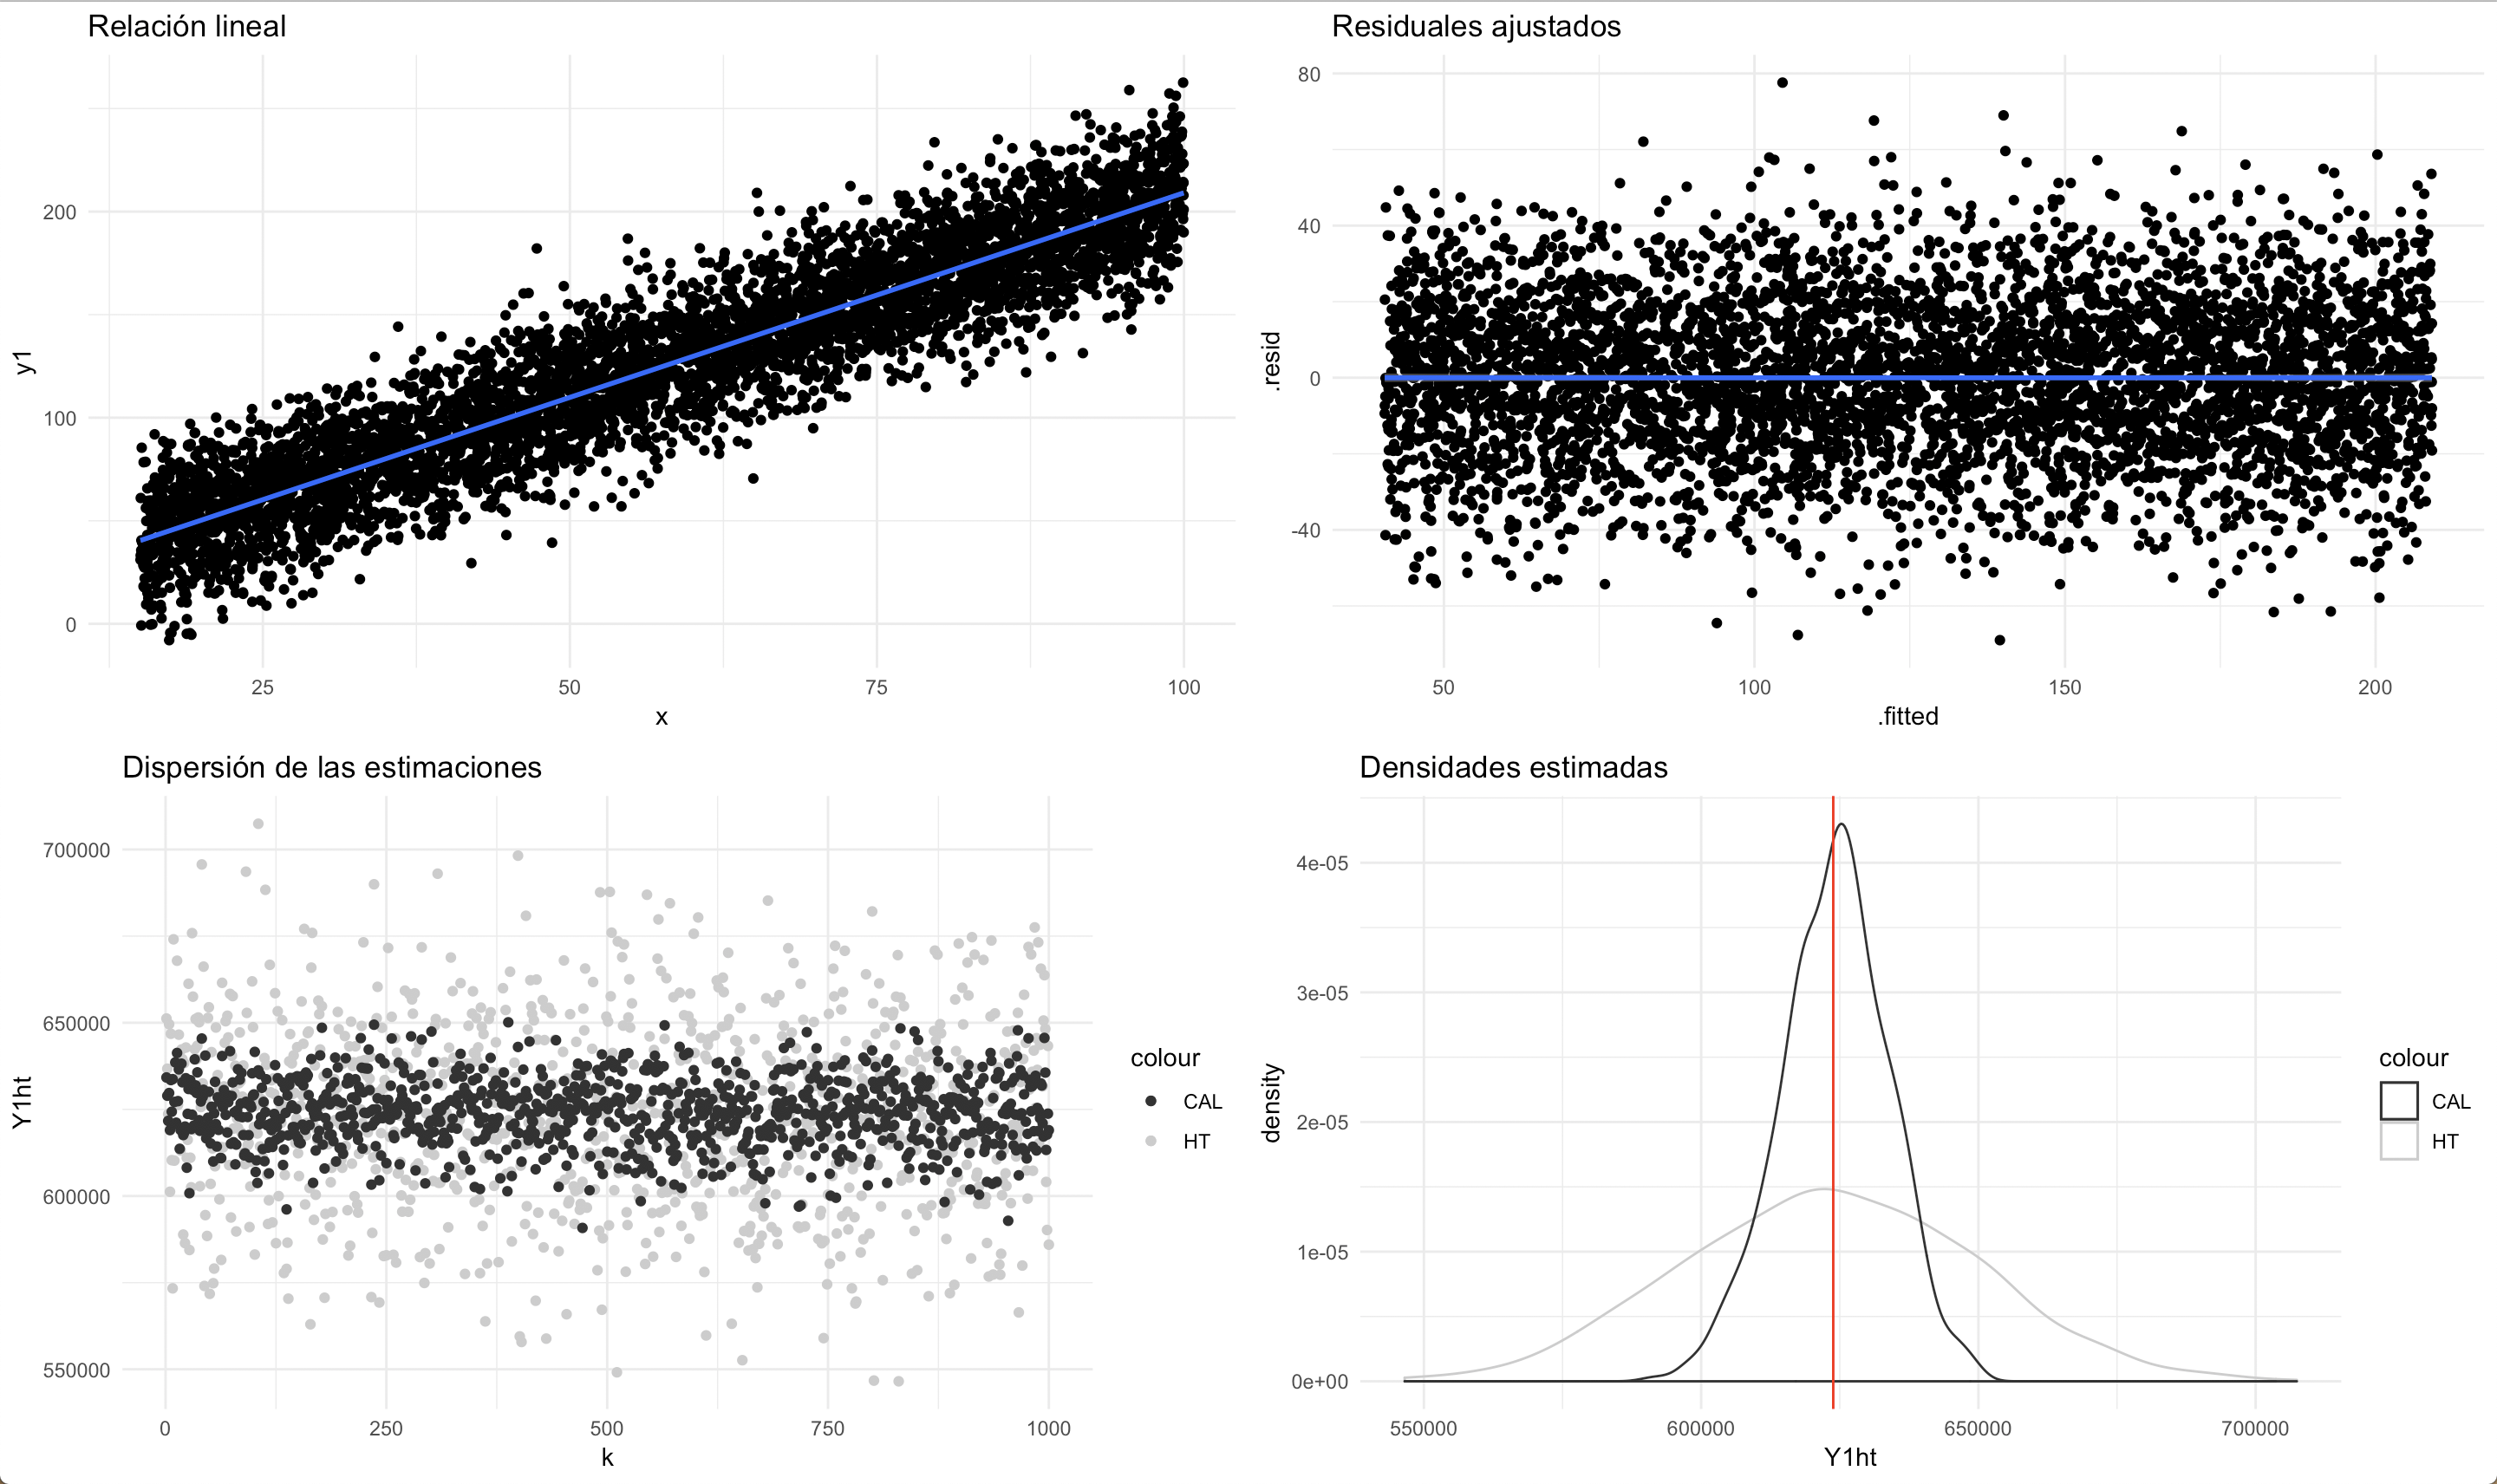
\includegraphics{Pics/c5.png}
\caption{\emph{Comportamiento del estimador de calibración en una relación de dependencia lineal}}
\end{figure}

El segundo conjunto de datos asume que existe una relación lineal entre la característica de interés y una variable de información auxiliar continua. Se nota que existe heteroscedasticidad en el modelo y los residuales lo muestran. A pesar de que ambos estimadores se muestran insesgados para el parámetro de interés, el estimador de calibración es un poco más eficiente que el de Horvitz-Thompson.

\begin{figure}
\centering
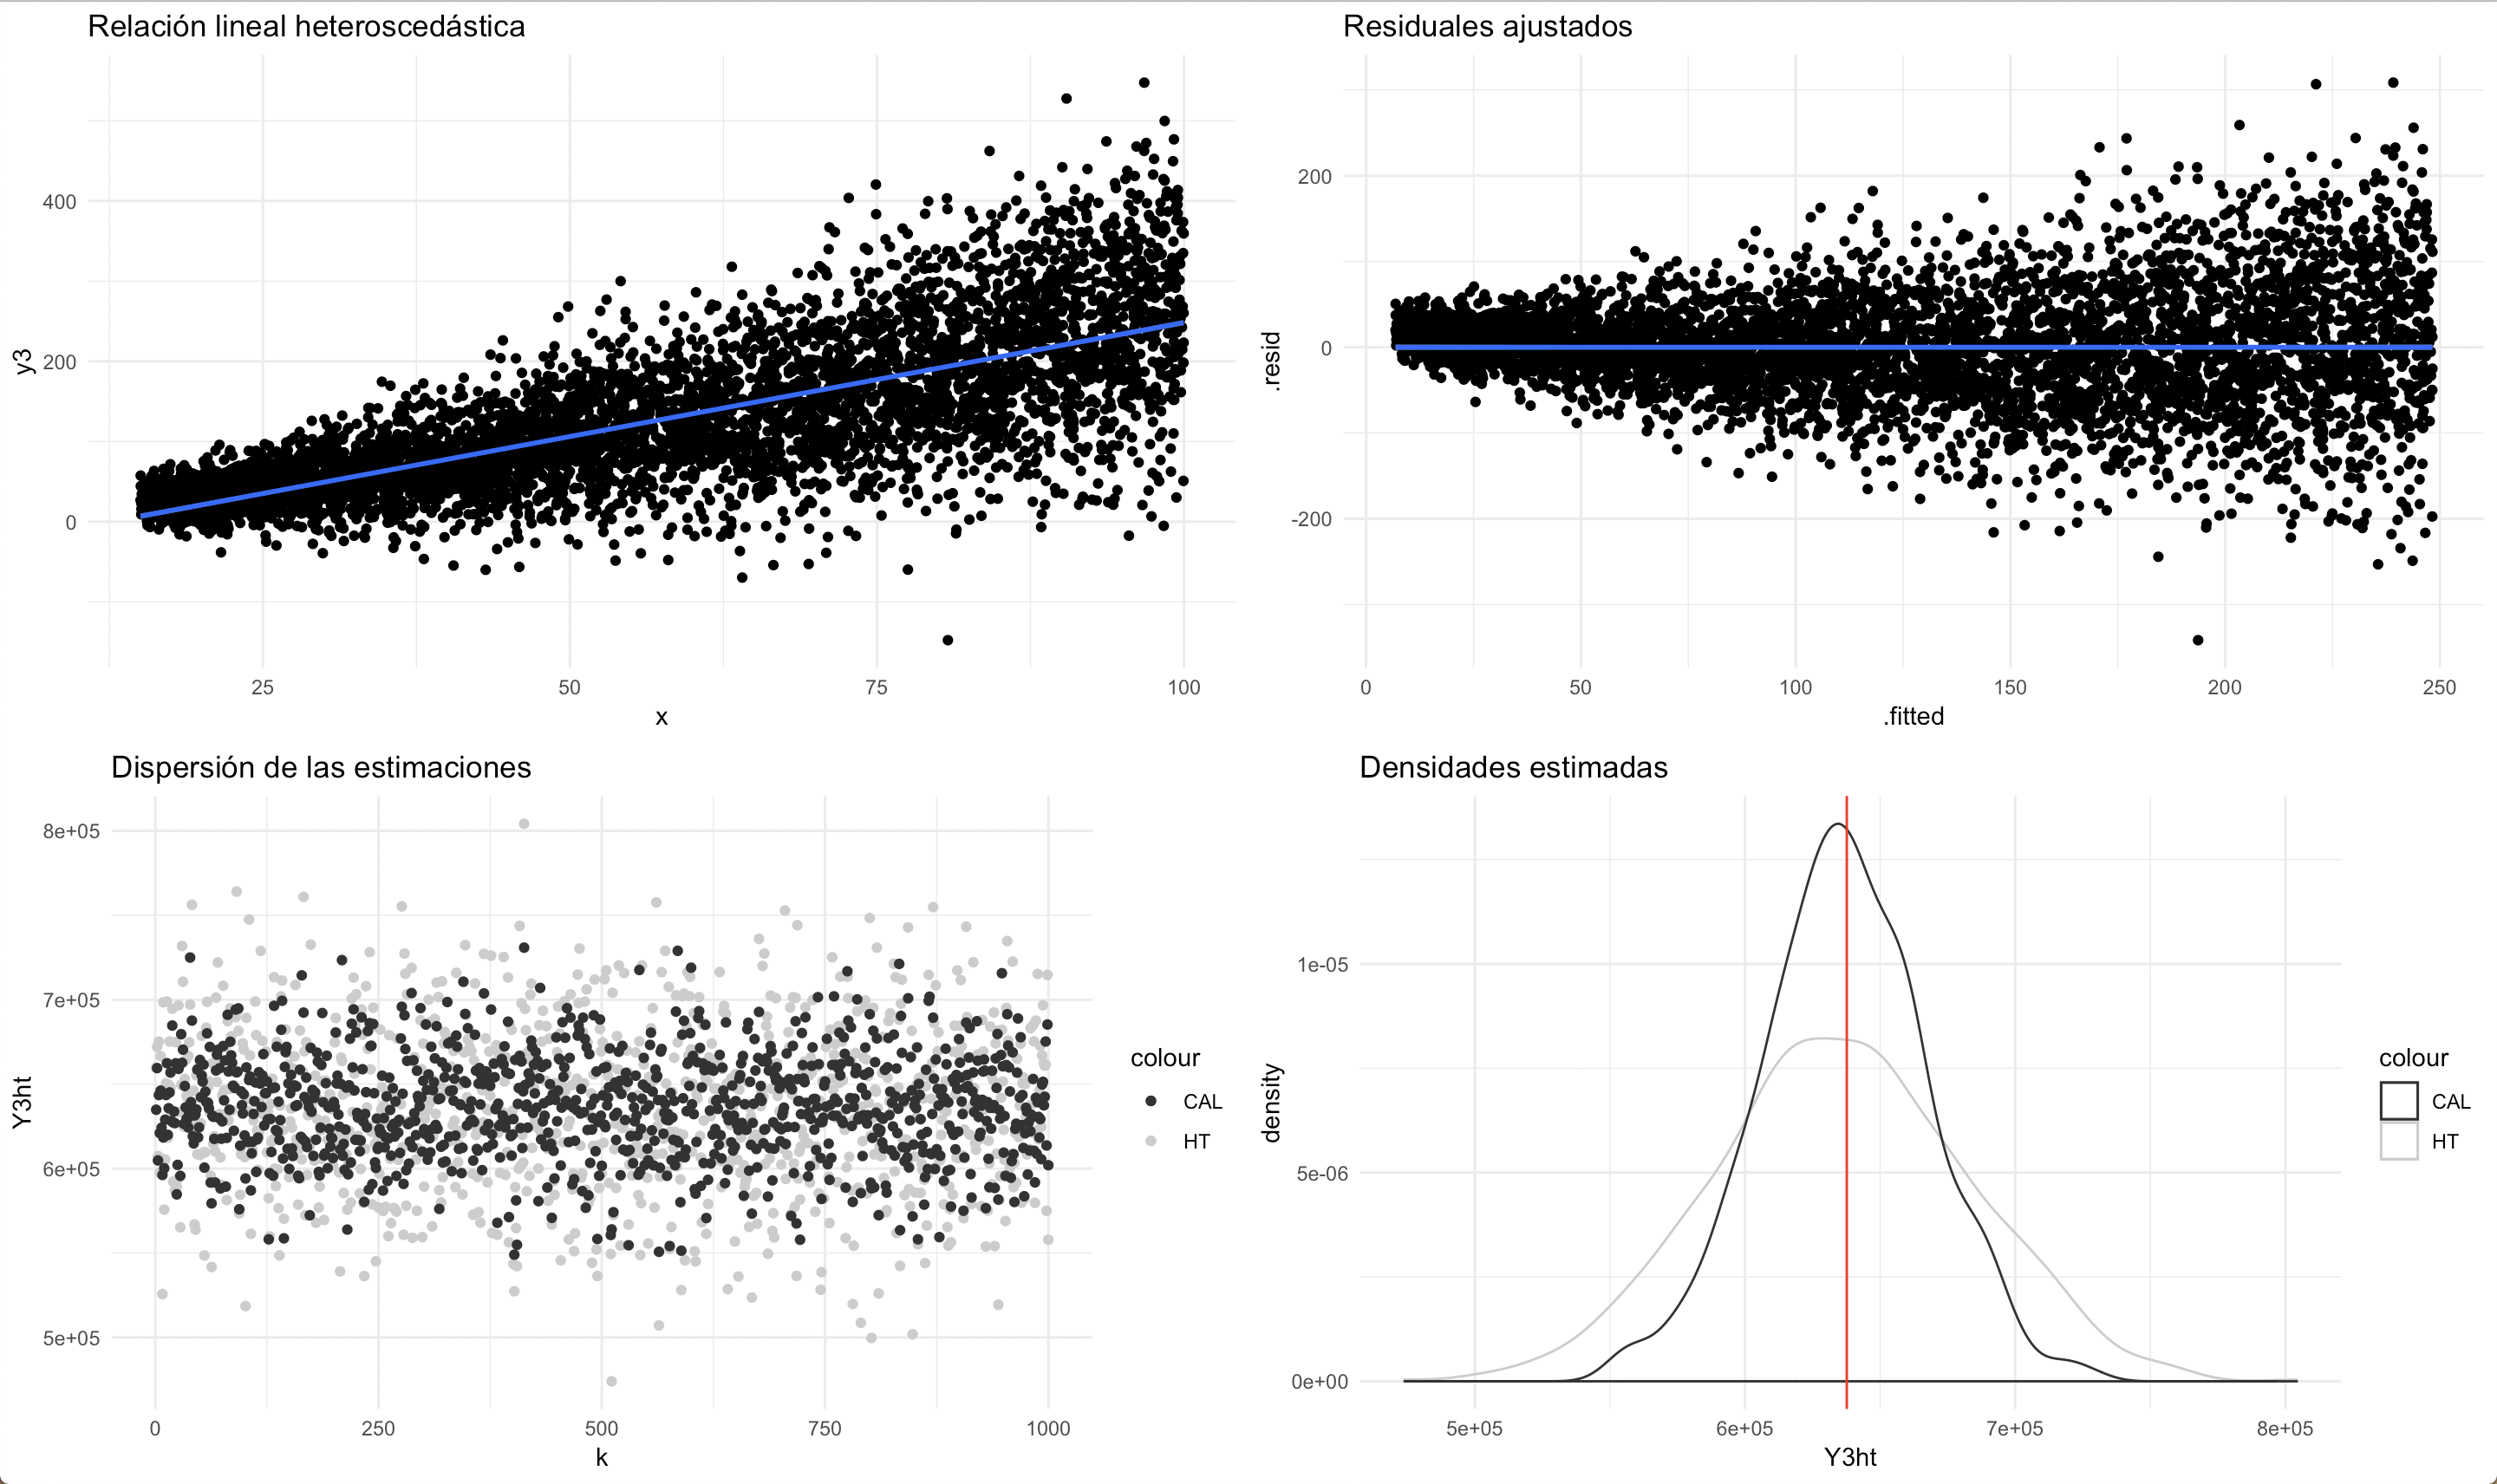
\includegraphics{Pics/c6.png}
\caption{\emph{Comportamiento del estimador de calibración en una relación de dependencia lineal con heteroscedasticidad}}
\end{figure}

El tercer conjunto de datos asume que existe una relación cuadrática entre la característica de interés y una variable de información auxiliar continua. Al utilizar un estimador de calibración lineal, los residuales muestran un comportamiento inapropiado. Sin embargo, ambos estimadores se muestran insesgados para el parámetro de interés, pero el estimador de calibración es más eficiente que el de Horvitz-Thompson.

\begin{figure}
\centering
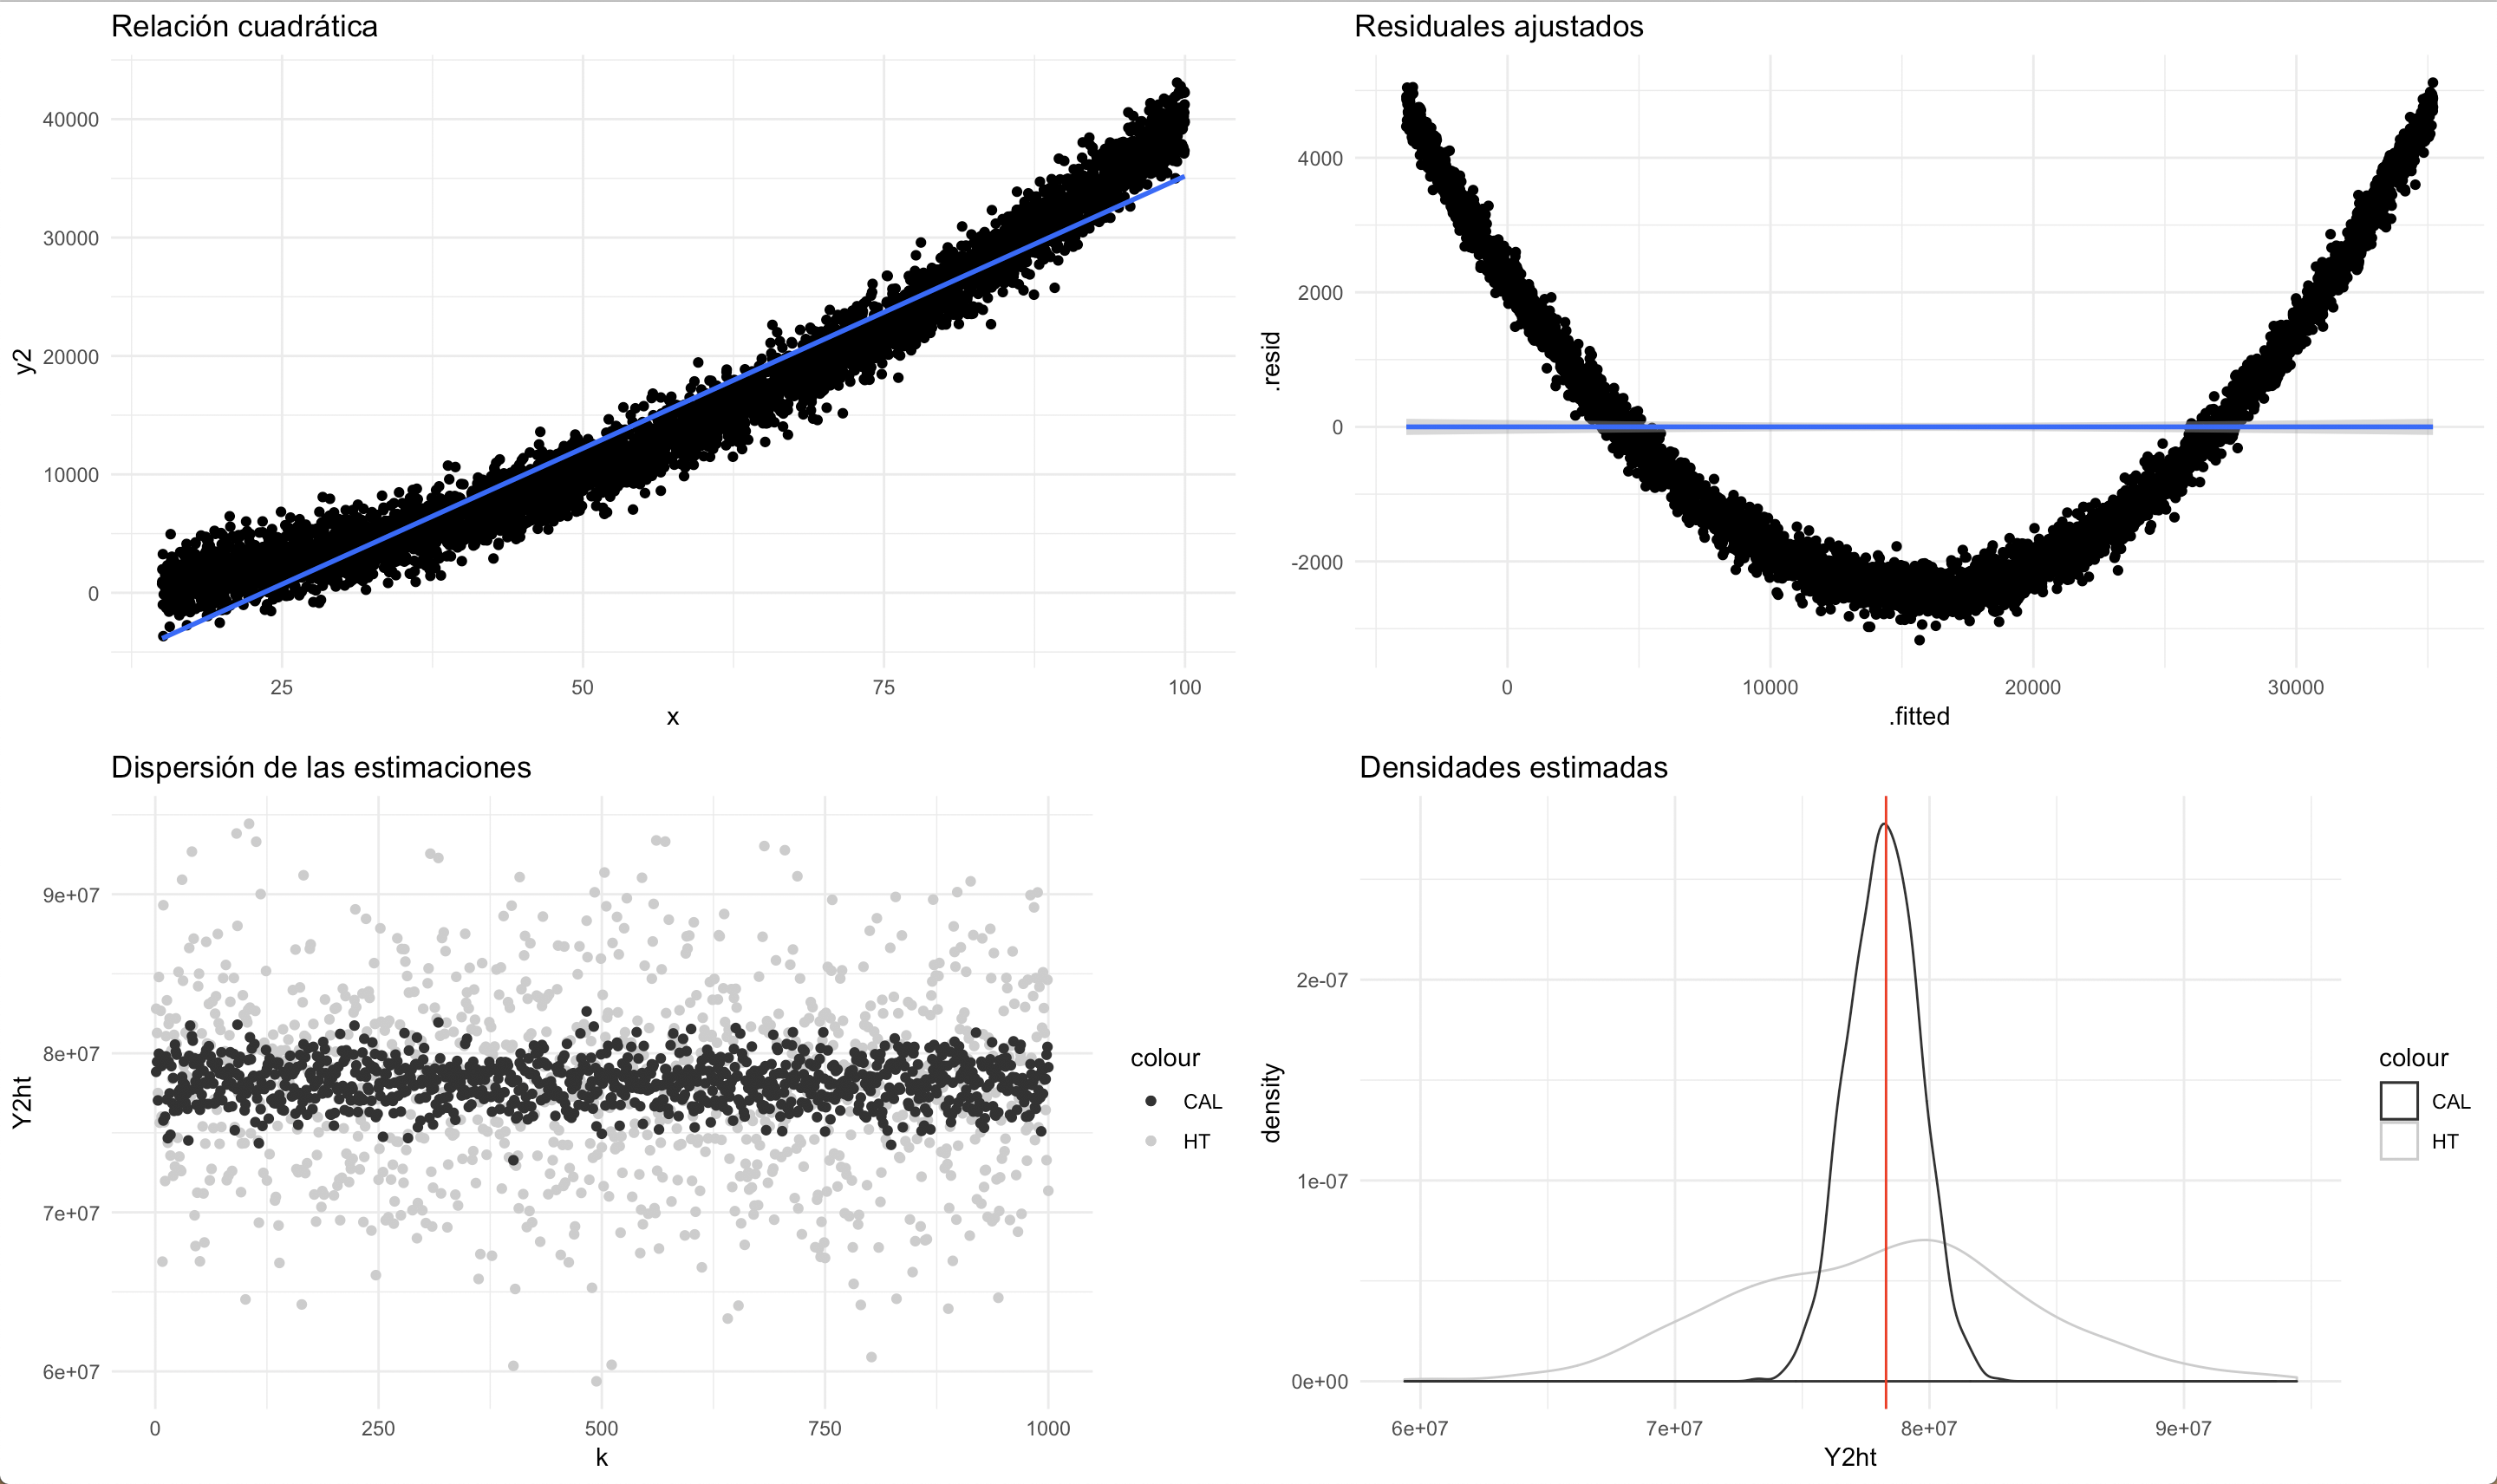
\includegraphics{Pics/c7.png}
\caption{\emph{Comportamiento del estimador de calibración en una relación de dependencia cuadrática}}
\end{figure}

El último conjunto de datos asume que existe una relación logística entre la característica de interés y una variable de información auxiliar dicotómica Al utilizar un estimador de calibración lineal, los residuales muestran un comportamiento inapropiado. Ambos estimadores se muestran insesgados para el parámetro de interés e igual de eficientes.

\begin{figure}
\centering
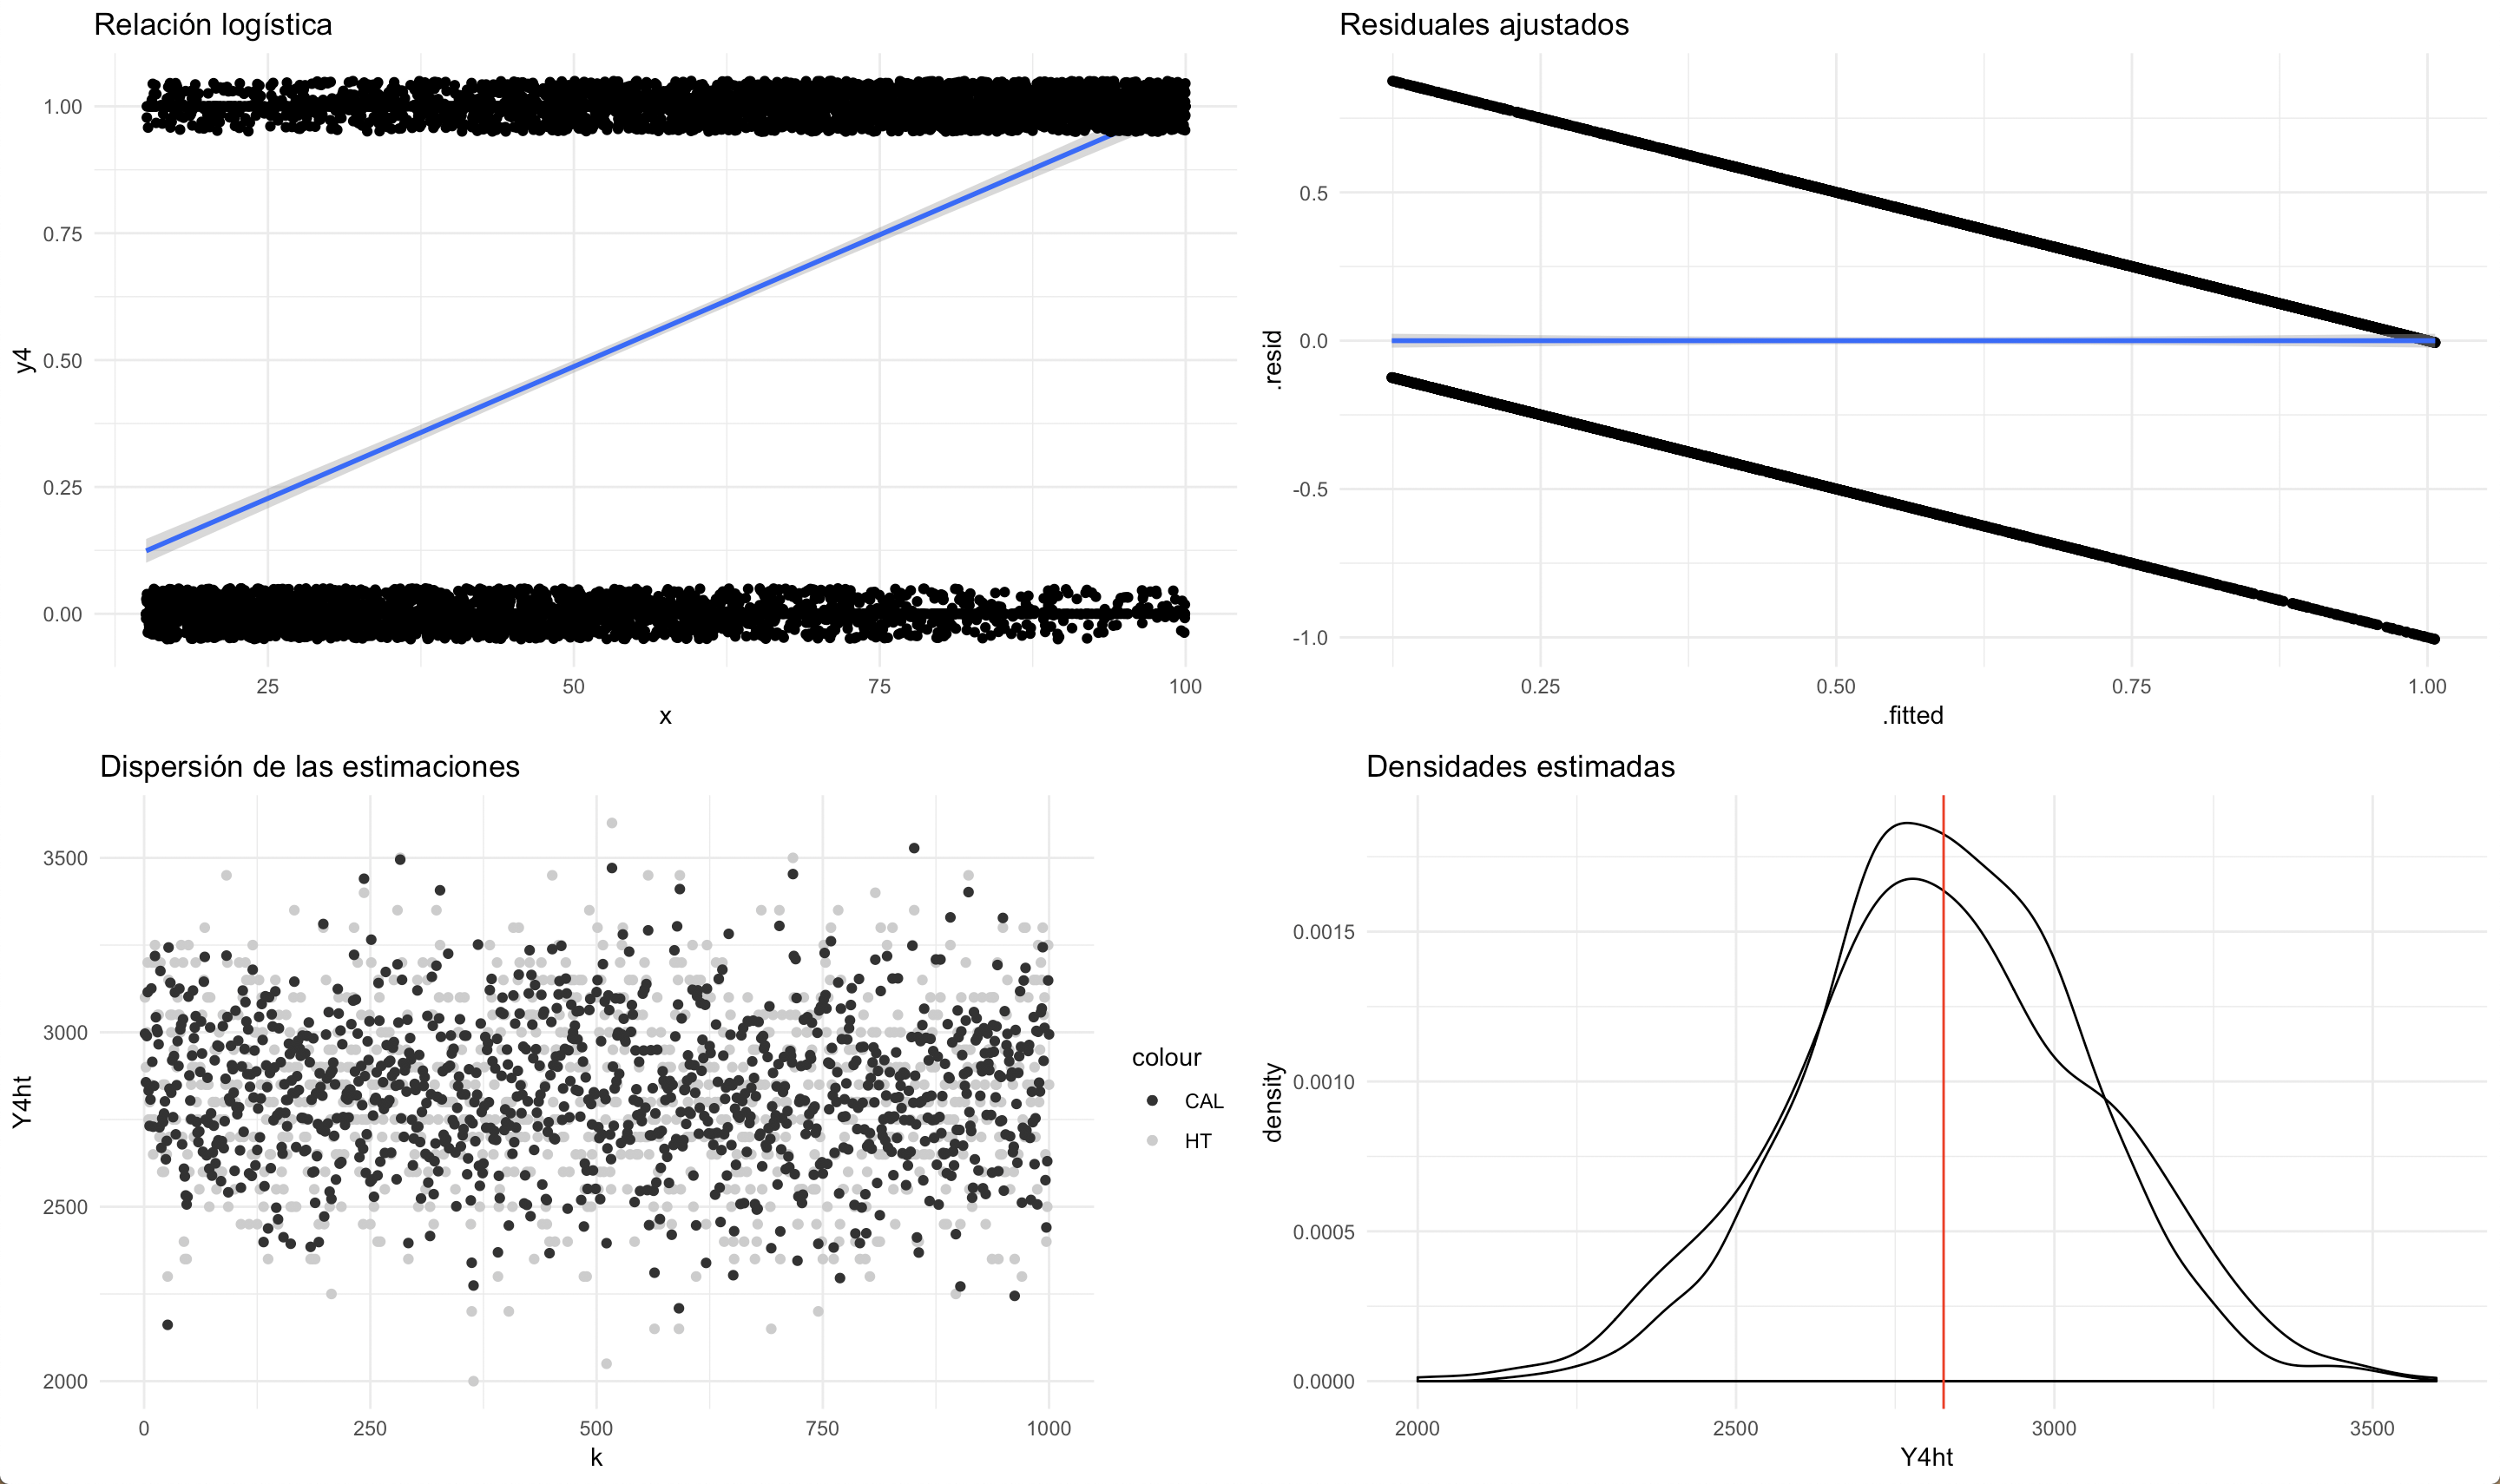
\includegraphics{Pics/c8.png}
\caption{\emph{Comportamiento del estimador de calibración en una relación de dependencia logística}}
\end{figure}

Es posible demostrar que la razón entre la varianza del estimador de calibración con la varianza del estimador de Horvitz-Thompson está supeditada al coeficiente de determinación \(R^2_{\xi}\) en un modelo de regresión lineal simple \(\xi\) entre la característica de interés y la información auxiliar.

\[
\frac{Var(\hat t_{y, cal})}{Var(\hat t_{y, HT})} = (1-R^2_{\xi} + o(\sqrt{n})) \approx (1-R^2_{\xi})
\]

Por ende, usar la metodología de calibración supone casi siempre una ganancia en la eficiencia de la estrategia de muestreo.

\hypertarget{diferentes-formas-del-estimador-de-calibraciuxf3n}{%
\subsection{Diferentes formas del estimador de calibración}\label{diferentes-formas-del-estimador-de-calibraciuxf3n}}

La calibración es un ajuste que se realiza a los pesos de muestreo con el propósito de que las estimaciones de algunas variables de control reproduzcan de forma perfecta los totales poblacionales de estas variables. Sin embargo, es necesario tener en cuenta las diferencias entre los métodos de calibración, que en general corresponderán con el nivel de desagregación de información auxiliar:

\begin{enumerate}
\def\labelenumi{\arabic{enumi}.}
\tightlist
\item
  Calibración con variables continuas, que es el caso en donde la calibración se realiza con totales de variables continuas como ingreso o gasto, entre otras.
\item
  Post-estratificación con variables categóricas, que representa el caso en donde la calibración se realiza con los tamaños poblacionales (basados en proyecciones demográficas o registros administrativos) de subgrupos de interés.
\item
  \emph{Raking} con variables categóricas, que se define como una calibración sobre los tamaños marginales de tablas de contingencia de subgrupos de interés. A diferencia del caso anterior, esta calibración no tiene en cuenta los tamaños de los cruces, sino solo los tamaños marginales; por ende, este método induce menos restricciones.
\end{enumerate}

\hypertarget{postestratificaciuxf3n}{%
\subsubsection{Postestratificación}\label{postestratificaciuxf3n}}

La postestratificación es una de las técnicas más usadas para el ajuste de los pesos de muestreo vía calibración. Este ajuste requiere la definición de categorías poblacionales. Por ejemplo, personas en un determinado grupo de edad, en cierta región y de cierta etnia o raza. Este método se implementa dentro de cada uno de los cruces inducidos por las covariables de interés (edad, región, etnia o raza). Nótese que, es necesario tener acceso a la información auxiliar a nivel de \emph{todos} los cruces definidos por los subgrupos. Usualmente corresponden a proyecciones demográficas. En este caso, la suma de los pesos ajustados reproducirán con exactitud los tamaños poblacionales en cada cruce.

Las categorías formadas para definir los pesos de muestreo se conocen como \emph{post-estratos} puesto que son definidas después de que la muestra es seleccionada y los datos son recolectados. Esta es una ventaja pues estas variables no necesariamente participan en la planificación del diseño de muestreo. Por ejemplo, en una encuesta de hogares es difícil estratificar por etnia o raza, edad, sexo o ciclo educativo alcanzado. Como se conoce que estas variables pueden estar correlacionadas con la pobreza, el ingreso o la ocupación, sería una buena idea contemplarlas en la calibración. Suponiendo que se definen cuatro categorías para la raza, dos para sexo, cinco para la edad, entonces habrían 40 post-estratos y sus respectivas restricciones.

De esta manera, siendo \(g = 1, \ldots, G\) el indicador del cruce poblacional (post-estrato), el estimador de postestratifiación queda definido de la siguiente manera:

\[
\hat{t}_{y, pos} = \sum_{g = 1}^G \frac{N_g}{\hat{N}_g}\hat{t}_{y_g}
\]

En donde \(N_g\) corresponde al tamaño poblacional del post-estrato, \(\hat{N}_g = \sum_{s_g} d_{k}\) y \(\hat{t}_{y_g} = \sum_{s_g} d_{k} y_k\). Por lo anterior, el factor de expansión de estimador postestratificado queda definido como sigue:

\[
w_k= d_k \frac{N_g}{\hat{N}_g} \ \ \ \ \ (k \in s_g)
\]

Note que \(d_k\) corresponde al peso inducido por el diseño de muestreo, corregido por los ajustes de elegibilidad y por la ausencia de respuesta, los cuales serán presentados en los capítulos posteriores del documento.

Por último, se debe considerar que la cantidad de postestratos en la calibración está inducido por la cantidad de interacciones en las variables auxiliares. En algunos casos, es posible encontrar cientos de interacciones. Aunque los tamaños de los postestratos se reproduce sin error, esto puede disminuir la eficiencia de la calibración en las variables de interés. Es decir, muchas variables e interacciones hacen que las estimaciones sean inestables, sobre todo si existen cruces con celdas vacías. Es posible que el efecto de las interacciones influencie la creación de los nuevos pesos calibrados y se tengan datos atípicos en los pesos de calibración resultantes.

\hypertarget{raking}{%
\subsubsection{Raking}\label{raking}}

¿Qué sucede si los conteos poblacionales (información auxiliar) no están disponibles para todos los cruces de las variables de calibración? Es posible que los agregados poblacionales de las variables provengan de distintas fuentes y no se pueda llegar a nivel de cruce. En este caso, es factible calibrar los marginales de la tabla cruzada, sin necesidad de calibrar todas sus entradas. En este caso, el número de restricciones decrecería con respecto a la postestratifación, pues se sumaría el número de categorías, mientras que en la postestratificación se multiplican. En el escenario anterior, en donde asumimos cuatro categorías para la raza, dos para sexo, cinco para la edad, entonces habrían únicamente 11 restricciones.

Para ajustar los marginales de la tabla cruzada, es necesario realizar un procedimiento iterativo (IPFP), el cual no tiene una escritura cerrada \citep[capítulo 10]{Gutierrez_2016}. Por ejemplo, si el \emph{raking} es de dos marginales, se ajustan primero las filas, luego las columnas y así sucesivamente hasta alcanzar la convergencia de los pesos calibrados y el procedimiento se detiene cuando se alcanza una tolerancia prefijada. Sin pérdida de generalidad, bajo este enfoque, los pesos calibrados se escriben de la siguiente manera:

\[w_k = d_k \times exp(u_h) \times exp(v_g)\]

En donde \(u_h\) es una función de los totales marginales de las filas de la tabla cruzada y \(v_g\) es una función de los totales marginales de las columnas. El \emph{raking} permite utilizar variables que pueden ser predictoras de las variables de interés o explicar la probabilidad de responder del hogar (o persona), además de paliar los efectos nocivos que las bajas tasas de cobertura del marco de muestreo conllevan sobre la inferencia.

\hypertarget{la-calibraciuxf3n-como-un-cambio-de-paradigma-en-una-teoruxeda-de-estimaciuxf3n-exhaustiva}{%
\subsection{La calibración como un cambio de paradigma en una teoría de estimación exhaustiva}\label{la-calibraciuxf3n-como-un-cambio-de-paradigma-en-una-teoruxeda-de-estimaciuxf3n-exhaustiva}}

\citet{Sar08} concluye que existen algunas ideas sobre las cuales vale la pena profundizar un poco más. A continuación se reproducen las ideas de \citet{Gutierrez_2016} sobre estos criterios para enfatizar el uso práctico de los estimadores de calibración:

\begin{quote}
\begin{quote}
\begin{enumerate}
\def\labelenumi{\arabic{enumi}.}
\tightlist
\item
  \emph{La calibración no se puede separar de la práctica.} El uso de los métodos de ponderación de las ONE es una costumbre que tiene sus orígenes en la ponderación de unidades mediante el inverso de su probabilidad de inclusión y continuó con las ponderaciones surgidas del enfoque de post-estratificación. Las ponderaciones de calibración extienden las anteriores ideas. Aunque la calibración aparece recientemente en la literatura, no lo es como técnica para producir ponderaciones.
\end{enumerate}
\end{quote}
\end{quote}

\begin{quote}
\begin{quote}
\begin{enumerate}
\def\labelenumi{\arabic{enumi}.}
\setcounter{enumi}{1}
\tightlist
\item
  \emph{La calibración no puede separarse de la consistencia estética\footnote{En este apartado la palabra consistente se da en el sentido de que el estimador reproduce exactamente los totales de la información auxiliar.}.} Las ecuaciones de calibración imponen esta propiedad de consistencia sobre el vector de ponderaciones; así que, cuando éste se aplica a las variables auxiliares el resultado será consistente con los totales de estas variables. El deseo de promover la credibilidad en las estadísticas oficiales es una razón para que las entidades busquen este tipo de consistencia.
\end{enumerate}
\end{quote}
\end{quote}

\begin{quote}
\begin{quote}
\begin{enumerate}
\def\labelenumi{\arabic{enumi}.}
\setcounter{enumi}{2}
\tightlist
\item
  \emph{La calibración debe ser de fácil interpretación.} El enfoque de calibración ha ganado popularidad en las aplicaciones reales debido a que las estimaciones resultantes son fáciles de interpretar y de motivar puesto que están directamente relacionadas a los pesos inducidos por el diseño de muestreo. La calibración sobre los totales conocidos brinda al usuario una forma natural y transparente de estimación. El usuario que entiende la ponderación muestral aprecia el método de calibración puesto que modifica sutilmente los pesos originales, pero al mismo tiempo respeta los totales de la información auxiliar. Además, la calibración induce un único vector de ponderaciones aplicable a todas las variables involucradas en el estudio. Esta última razón hace que este método sea muy apetecido en las entidades oficiales que manejan encuestas muy extensas.
\end{enumerate}
\end{quote}
\end{quote}

\begin{quote}
\begin{quote}
\begin{enumerate}
\def\labelenumi{\arabic{enumi}.}
\setcounter{enumi}{3}
\tightlist
\item
  \emph{La calibración representa un enfoque exhaustivo y unificado basado en los avances de teorías anteriores.} En la práctica de las enceustas de hogares, es cpmún encontrar problemas como la ausencia de respuesta, deficiencias del marco muestral y errores de medición. Aunque algunos procesos como la imputación y la reponderación son ampliamente difundidos y usados en la práctica, estos métodos no están necesariamente enmarcados dentro de una teoría exhaustiva de inferencia en poblaciones finitas. La mayoría de artículos teóricos tratan con la estimación de parámetros bajo un mundo ideal, que no existe en la práctica, donde la ausencia de respuesta y otros errores no muestrales están ausentes. La calibración proporciona una teoría unificada que hace frente a estos inconvenientes.
\end{enumerate}
\end{quote}
\end{quote}

\hypertarget{estimadores-compuestos}{%
\section{Estimadores compuestos}\label{estimadores-compuestos}}

Es posible mejorar la estimación del total actual \(t_y^{(t)}\) al tener en cuenta la información inducida por el traslape\footnote{En esta sección, la notación para la parte traslapada \(s_M\) de la muestra actual usará el superíndice \(M\) (\emph{matched}); mientras que se utilizará el superíndice \(U\) (\emph{unmatched}) para refereirse a la parte no traslapada \(s_U\) de la muestra actual.} de la encuesta en el segundo periodo, así:

\[
\hat{t}_{y^{(t)}}^K = (1-K) \hat{t}_{y^{(t)}} 
+ K (\hat{t}_{y^{(t-1)}} + \hat{\Delta}_M)
\]

En donde \(0 < \alpha < 1\) y \(\hat{\Delta}_M=\hat{t}_{y^{(t)}}^M - \hat{t}_{y^{(t-1)}}^M\) es la diferencia de las estimaciones actual y previa en la muestra traslapada. Por otro lado, es posible añadir un término que dé cuenta de la diferencia entre las estimaciones actuales de las muestras con y sin traslape. De esta forma, un estimador compuesto es el siguiente:

\[
\hat{t}_{y^{(t)}}^{AK} = \hat{t}_{y^{(t)}}^K + A  (\hat{t}_{y^{(t)}}^U - \hat{t}_{y^{(t)}}^M)
\]

\citet{Steel_McLaren_2008} afirman que esta clase de estimadores pueden generar ganancias en eficiencia porque aprovechan la correlación entre las estimaciones del mismo panel a lo largo del tiempo y puede otorgar una ventaja adicional a la estimación tradicional que utiliza únicamente la muestra actual como un todo, sin detenerse en su composición: parte traslapada y parte no traslapada. Estos estimadores pueden usar diferentes valores para las constantes \(A\) y \(K\), las cuales pueden ser escogidas con el objetivo de minimizar la varianza del estimador, o pueden ser escogidas de forma separada para aumentar la eficiencia del estimador con respecto a estimadores de niveles, como totales o proporciones del periodo actual, o de cambios temporales. \citet{Gurney_Daly_1965} utilizan \(A=0.4\) y \(K=0.2\) en una aplicación con paneles rotativos.

Estos estimadores también pueden ser escritos como estimadores de regresión o calibración. En efecto, \citet{Gambino_Kennedy_Singh_2001} proponen que, además de las covariables y restricciones de calibración usuales, es posible usar la siguiente covariable de calibración para estimar indicadores de nivel:

\[
x_k^{(l)} = 
\begin{cases}
\hat {\bar y} ^{(t-1)}, \ \ \ \ \ k \in s_U \\
y_{k}^{(t-1)}, \ \ \ \ \ k \in s_M 
\end{cases}
\]

Por ejemplo, si el interés está en la estimación de la proporción actual de personas ocupadas, entonces \(x_k^{(l)}\) representará la covariable que se deberá añadir al sistema de calibración, \(\hat {\bar y} ^{(t-1)}\) será la proporción estimada de personas ocupadas en el periodo anterior, mientras que \(y_{k}^{(t-1)}\) representará una variable dicotómica sobre la población económicamente activa que toma el valor uno, si la persona estuvo ocupada en el periodo anterior, o cero, si no. En este caso, el total de control correspondiente estará definido por el total nacional estimado de personas ocupadas en el periodo anterior. Por lo tanto, como es de esperarse, la suma ponderada (con los pesos de calibración) de esta covariable deberá ser igual a su total de control.

Para estimadores de cambio, \citet{Gambino_Kennedy_Singh_2001} proponen la siguiente covariable:

\[
x_k^{(c)} = 
\begin{cases}
y_{k}^{(t)}, \ \ \ \ \ \ \ \ \ \ \ \ \ \ \ \ \ \ \ \ \ \ \ \ \ \ \ \ \ \ \ \ \ \ \ \ \ \ \ \ k \in s_U \\
y_{k}^{(t)} - R(y_{k}^{(t)} - y_{k}^{(t-1)}), \ \ \ \ \ k \in s_M 
\end{cases}
\]

En donde \(R = \sum_s w_k / \sum_{s_M} w_k\) es el inverso de la proporción de traslape real en el levantamiento. Siguiendo con el ejemplo, \(y_{k}^{(t)}\) representa una variable dicotómica sobre la población económicamente activa que toma el valor uno, si la persona estuvo ocupada en el periodo actual, o cero, si no. En este caso, el total de control correspondiente sigue estando definido por el total nacional estimado de personas ocupadas en el periodo anterior. Por lo tanto, al sumar sobre la muestra expandida, se presenta la siguiente relación \(\hat{t}_{y^{(t-1)}} = \hat{t}_{y^{(t)}} - \hat{\Delta}_M)\); es decir, que la estimación del periodo anterior es igual a la estimación del mes actual menos una diferencia de estimaciones en la muestra traslapada.

Es posible usar ambas covariables \(x_k^{(c)}\) y \(x_k^{(l)}\) en el sistema de calibración, aunque es probable sea encontrar pesos resultantes negativos o menores que uno. Para evitar estos inconvenientes numéricos, y dado que para ambas variables se tiene el mismo total de control, es posible definir una combinación lineal convexa y crear una nueva covariable de calibración, de la siguiente manera:

\[
x_k = (1-\alpha) x_k^{(l)} + \alpha x_k^{(c)}
\]

\citet{Fuller_Rao_2001} mencionan que en algunas aplicaciones particulares, se ha encontrado mayor eficiencia (menor varianza) al utilizar valores de \(\alpha = 0.65\) o \(\alpha = 0.75\); aunque se recomienda usar \(\alpha = 2/3\) en los sistemas de producción de las ONE.

\citet{Gambino_Kennedy_Singh_2001} afirman que existe una facilidad en la implementación de estos estimadores puesto que se corresponde con la manera usual de un sistema tradicional de ponderación en las encuestas de hogares; es decir, se crea una columna nueva en la base de datos definiendo el nuevo factor de expansión, y esto se logra simplemente con la adición de nuevas covariables a la matriz de calibración.

En América Latina, El Instituto Nacional de Estadística del Uruguay, decidió rediseñar en 2021 la Encuesta Continua de Hogares en 2019, la cual estaba definida desde el 2006 con base en la selección de muestras mensuales independientes. En la metodología nueva, se implementó un sistema de panel rotativo, en donde la muestra de un mes está compuesta por seis grupos de rotación y la recolección de la información tiene un carácter mixto: para la recolección de la información en la primera visita, de forma presencial y, para el seguimiento durante los siguientes cinco meses, de forma telefónica. Además, el INE implementó un sistema de estimación basado en los estimadores compuestos con mejoras en la eficiencia estadística \citep{INEURY}

\hypertarget{construcciuxf3n-de-los-factores-de-expansiuxf3n}{%
\chapter{Construcción de los factores de expansión}\label{construcciuxf3n-de-los-factores-de-expansiuxf3n}}

En todas las bases de datos de las encuestas de hogares se encuentra una columna que contiene los pesos de muestreo o factores de expansión. Con esta columna se realizan todos los análisis requeridos en la encuesta, desde estimar medias, razones, tamaños y proporciones hasta el ajuste de modelos lineales y no lineales. La razón principal por la cual se usan los factores de expansión es para producir estimaciones que reflejen de manera precisa el comportamiento de la población objetivo. El uso correcto de los factores de expansión garantiza que la estimación sea insesgada y consistente, que el error de muestreo sea pequeño, condicionado al diseño muestral y al tamaño de la muestra; además de corregir las deficiencias de cobertura del marco de muestreo.

La naturaleza de los factores de expansión es intuitiva y se da en el marco del principio de representatividad que gobierna la inferencia de las encuestas de hogares y cualquier otra operación estadística basada en la selección de una muestra. De esta forma, el factor de expansión de una unidad muestral representa el número de veces que se representa a sí misma y a otras unidades similares a ella misma. En general, bajo condiciones de regularidad, el factor de expansión será siempre positivo y mayor que la unidad. Además, la suma de los factores de expansión sobre la base de datos deberá ser aproximarse al tamaño de la población sobre la cual se desea realizar la inferencia.

Por ejemplo, un hogar en una encuesta con un factor de expansión de 500 se representa a sí mismo y a otros 499 hogares más. La definición teórica del factor de expansión, inducida por el inverso multiplicativo de la probabilidad de inclusión de un hogar en la muestra, hace que la inferencia sea insesgada y confiable. Sin embargo, debido a que la probabilidad de inclusión es un número real contenido en el intervalo \((0, 1]\), entonces su inverso multiplicativo también será un número real mayor o igual que uno. Asimismo, si en el país hay alrededor de cuatro millones de hogares, se espera que la suma de los factores de expansión sobre la muestra de hogares esté alrededor de esta cifra.

Los procesos de inferencia estadística establecidos en cualquier encuesta de hogares descansan sobre el principio de representatividad que afirma que es posible seleccionar una muestra y representar con bastante precisión y exactitud la realidad de la población de interés. A su vez, las propiedades estadísticas de la inferencia en encuestas de hogares descansan sobre las probabilidades de inclusión generadas por el diseño de muestreo que se implementó en la encuesta. En general el peso de muestreo \(d_k\) asociado a un individuo \(k\) en la muestra \(s\) es función de la probabilidad de inclusión del individuo, así:

\[
d_k = \frac{1}{Pr(k\in s)}
\]

Como se mencionó anteriormente, para conservar la estabilidad en los pesos de muestreo, es posible definir diseños de muestreo auto-ponderados, en donde las unidades finales de muestreo tengan las misma probabilidad de inclusión, sin importar el tamaño de la unidad primaria de muestreo que la contiene. Este tipo de diseños es útil porque induce mayor control sobre las estimaciones finales. Además, \citet{Valliant_Dever_2017} afirman que los pesos de muestreo se utilizan con el fin de incorporar las probabilidades de selección de las unidades en la muestra, ajustar en casos en los que no se pueda determinar si algunas unidades en la muestra son miembros de la población de interés, minimizar el sesgo causado por la ausencia de respuesta cuando algunas unidades no responden habiendo sido incluidas en la muestra, incorporar información auxiliar externa para reducir los errores muestrales de las estimaciones y compensar cuando la muestra no cubre correctamente a la población de interés.

Es de notar que la conformación de los pesos de muestreo se transforma en un reto metodológico para el investigador, puesto que debe ajustarse a la realidad de la región en donde las poblaciones de los municipios se expanden cada vez más en el sector urbano y los marcos de muestreo de las áreas geográficas se desactualizan con rapidez. Varias soluciones a este problema han sido planteadas \citep{Gambino_Silva_2009} y todas ellas requieren de esfuerzos económicos, logísticos y técnicos. Por ende, los equipos de los INE (a todo nivel) deben ser flexibles y adecuarse a esta realidad cambiante de la movilidad de las poblaciones, sobre todo en las áreas urbanas.

En condiciones ideales el marco de muestreo debería coincidir plenamente con la población finita. Sin embargo, en general, no es posible contar con una lista de todos los elementos de la población y, en el contexto de las encuestas a hogares, no existe una lista que enumere todos los hogares de un país de manera actualizada, por lo que la práctica estándar es construir el marco de muestreo en varias etapas, seleccionando una muestra de áreas geográficas, realizando un empadronamiento exhaustivo de todos los hogares en las áreas seleccionadas y luego seleccionando hogares. Este esquema de muestreo hace que el marco de muestreo de las encuestas a hogares presente imperfecciones.

Para hacerle frente a las imperfeccciones del marco, \citet{Valliant_Dever_2017} recomienda el uso de los códigos de disposición estandarizados por la \emph{American Association for Public Opinion Research} (AAPOR) recomienda tratar la ausencia de respuesta de manera diferenciada y clasificar a cada unidad en la muestra en algunas de las siguientes categorías:

\begin{enumerate}
\def\labelenumi{\arabic{enumi}.}
\tightlist
\item
  ER (\emph{elegible respondents}), unidades elegibles que fueron respondientes efectivos que denotan casos elegibles para los cuales se ha recolectado una cantidad suficiente de información.
\item
  ENR (\emph{elegible nonrespondents}), unidades eligibles no respondientes que denotan los casos elegibles para los cuales no se recolectó ningún dato o la información fue parcialmente recolectada.
\item
  IN (\emph{ineligibles}), unidades no elegibles que conforman los casos de miembros no elegibles que no hacen parte de la población de interés.
\item
  UNK (\emph{unknown elegibility}), unidades con elegibilidad desconocida que denotan los casos en donde no se puede conocer si la unidad es elegible o no.
\end{enumerate}

Para construir los factores de expansión de una encuesta se recomienda seguir en este orden los siguientes procesos:

\begin{enumerate}
\def\labelenumi{\arabic{enumi}.}
\tightlist
\item
  Creación de los pesos básicos.
\item
  Ajuste por elegibilidad desconocida.
\item
  Descarte de las unidades no elegibles.
\item
  Ajuste por ausencia de respuesta.
\item
  Calibración por proyecciones poblacionales y variables auxiliares.
\item
  Recorte y redondeo de los factores finales (\emph{opcional}).
\end{enumerate}

\hypertarget{creaciuxf3n-de-los-pesos-buxe1sicos}{%
\section{Creación de los pesos básicos}\label{creaciuxf3n-de-los-pesos-buxe1sicos}}

Este primer paso ya ha sido explicado de forma detallada en el capítulo dedicado a la selección de la muestra. Observe que, asociado a cada esquema particular de muestreo, existe una única función que vincula a cada elemento con una probabilidad de inclusión en la muestra. De esta forma:

\[\pi_k = Pr (k \in s)\]

Por lo tanto, el primer paso en la reponderación de los pesos de muestreo, es justamente la creación de los pesos básicos \(d_{1k}\) que se definen como el inverso multiplicativo de la probabilidad de inclusión

\[d_{1k} = \frac{1}{\pi_k}  \ \ \ \ \ \ \ \ \forall \ k\in s\]

Estos pesos son creados incluso para aquellas unidades que serán excluidas de la muestra porque son no elegibles o porque no proveyeron ninguna información y luego serán modificados convenientemente. La siguiente figura muestra la distribución típica de los pesos originales en una encuesta de hogares. Se recomienda calcular las probabilidades de inclusión (si el muestreo es sin reemplazo) o selección (si el muestreo es con reeemplazo) a medida que avance el muestreo en sus etapas y, de esta forma, siempre confirmar la consistencia de los pesos en cada etapa y de los pesos finales.

A través de las modificaciones posteriores sobre este peso de muestreo, la distribución de los ponderadores irá sufriendo algunos cambios. Si la distribución original de los pesos básicos difiere estructuralmente con la distribución final de los ponderadores, resultante de todos los ajustes debidos a las imperfecciones del marco, entonces las propiedades estadísticas de insesgamiento, consistencia y precisión podrían desvanecerse. Lo anterior implica que el nivel de desactualización del marco de muestreo tiene implicaciones directas en la calidad de la inferencia. Por tanto, si el marco de muestreo es muy imperfecto, los ponderadores finales no inducirán una inferencia precisa.

\hypertarget{ajuste-por-elegibilidad-desconocida}{%
\section{Ajuste por elegibilidad desconocida}\label{ajuste-por-elegibilidad-desconocida}}

El segundo paso consiste en redistribuir el peso de las unidades cuyo estado de elegibilidad es desconocido. Por ejemplo, si la encuesta está enfocada en la población mayor de 15 años y hay personas que no proveen ninguna información acerca de su edad, entonces es necesario distribuir estos pesos. Esta situación también se puede presentar a nivel de hogar cuando no puede ser contactado porque nadie nunca atendió el llamado del encuestador (\emph{nadie en casa}). Se acostumbra a redistribuir los pesos de las unidades con elegibilidad desconocida (UNK) entre las unidades que sí disponen de su estatus de elegibilidad (ER, ENR, IN).

Por consiguiente, si no es posible determinar la elegibilidad de algunas unidades que aparecen en el marco de muestreo, se tendrá una muestra \(s\) que contendrá el subconjunto de las unidades \emph{elegibles respondientes} \((s_{ER})\), el subconjunto de las unidades \emph{elegibles no respondientes} \((s_{ENR})\), el subconjunto de las unidades \emph{no elegibles} \((s_{IN})\) y el subconjunto de las unidades con \emph{elegibilidad desconocidad} \((s_{UKN})\). En este último caso, la elegibilidad de estas unidades se mantiene desconocida, a no ser que de manera arbitraria sean clasificadas como ENR (elegibles no respondientes), o se tenga información auxiliar en el marco de muestreo que permita imputar su estado de elegibilidad.

Se recomienda formar \(B\) \((b = 1, \ldots, B)\) categorías\footnote{\citet{Valliant_Dever_2017} recomienda formar categorías con al menos 50 casos.} basadas en la información del marco de muestreo. Estas categorías pueden ser estratos o cruces de subpoblaciones. Siendo \(s_b\) la muestra de unidades en la categoría \(b\) (que incluye a ER, ENR, IN y UNK), se define el factor de ajuste por elegibilidad como:

\[
a_b = \frac{\sum_{s_b}d_{1k}}{\sum_{s_b \cap (s_{ER} \cup s_{ENR} \cup s_{IN})}d_{1k}}
\]
Para la categoría \(b\), los pesos ajustados por elegibilidad desconocida para aquellas unidades cuya elegibilidad sí pudo ser establecida (independientemente de su estado de respuesta) estarán dados por la siguiente expresión:

\[
d_{2k} = a_b * d_{1k}  \ \ \ \ \ \ \ \ \forall \ k\in s_b \cap (s_{ER} \cup s_{ENR} \cup s_{IN})
\]

\hypertarget{descarte-de-las-unidades-no-elegibles}{%
\section{Descarte de las unidades no elegibles}\label{descarte-de-las-unidades-no-elegibles}}

En esta etapa, tanto las viviendas con elegibilidad desconocida (UNK) como las viviendas que han cambiado su estado de ocupación y ahora no contienen ningún hogar particular (IN) se retirarán de la población objetivo. Por ende, la base de datos sobre la cual se prosigue el proceso ahora presentará una reducción en el número de unidades. Este tercer paso consiste en ajustar el peso de la etapa anterior de la siguiente manera:

\[
d_{3k} = 
\begin{cases}
0, \ \ \ \ \ \text{si la unidad $k \in (s_{UNK} \cup s_{IN})$ }\\
d_{2k},\ \ \ \text{si la unidad $k \in (s_{ER} \cup s_{ENR})$.}
\end{cases}
\]

\hypertarget{ajuste-por-ausencia-de-respuesta}{%
\section{Ajuste por ausencia de respuesta}\label{ajuste-por-ausencia-de-respuesta}}

En este paso los pesos de los respondientes efectivos (ER) se ajustan para tener en cuenta a los que no respondieron (ENR). Al final del proceso, los pesos de los ER se incrementan para compensar el hecho de que algunas unidades elegibles no proveyeron información. Para el manejo efectivo de la ausencia de respuesta se consideran las siguientes variables aleatorias:

\[
I_k=
\begin{cases}
1,  &\text{si $k \in (s_{ER} \cup s_{ENR})$}\\
0,  &\text{en otro caso.}
\end{cases}
\]

\[
D_k=
\begin{cases}
1,  &\text{si $k \in s_{ER}$}\\
0,  &\text{si $k \in s_{ENR}$.}
\end{cases}
\]

Al suponer que la distribución de las respuestas puede ser estimada, entonces la probabilidad de respuesta (\emph{propensity score}) está dada por

\[
Pr[ k\in s_{ER}|k\in (s_{ER} \cup s_{ENR})]=Pr[D_k = 1|I_k = 1]=\phi_k
\]

Si el patrón de ausencia de respuesta es completamente aleatorio (en donde la no respuesta no sigue ningún patrón específico) o aleatorio (en donde el patrón de la no respuesta puede ser explicado por un conjunto de covariables \(\mathbf{z}\)), entonces

\[
\phi_k = f(\mathbf{z}_k, \boldsymbol{\beta})   \ \ \ \ \ \ \ \ \forall \ k \in (s_{ER} \cup s_{ENR})
\]

De esta forma, si fuese plausible tener acceso a las covariables \(\mathbf{z}\) para los individuos elegibles en la muestra, entonces se podría estimar el patrón de ausencia de respuesta mediante la siguiente relación funcional:

\[
\hat{\phi}_k = f(\mathbf{z}_k, \hat{\boldsymbol{\beta}})   \ \ \ \ \ \ \ \ \forall \ k \in (s_{ER} \cup s_{ENR})
\]

Por otro lado, si el patrón de ausencia de respuesta es no aleatorio (en donde la misma estructura de la ausencia de respuesta es explicada por la variable de interés; por ejemplo cuando en una encuesta de mercado laboral son los desempleados quienes no responden), entonces

\[
\phi_k = f(\mathbf{y}_k, \beta)   \ \ \ \ \ \ \ \ \forall \ k \in (s_{ER} \cup s_{ENR})
\]

En este caso, como no es posible tener acceso a la variables de interés para todos los individuos en la muestra de unidades elegibles (precisamente porque no todos respondieron), entonces no es posible estimar el patrón de ausencia de respuesta y por ende habrán problemas de sesgo. Por otra parte, \citet{Kim_Riddles_2012} muestran que es posible utilizar un modelo basado de estimación de las probabilidades de respuesta (\emph{propensity score}). De esta forma, teniendo en cuenta que la probabilidad de que un individuo conteste es \(\phi_k = Pr(k \in s_{ER})\), al suponer que existe acceso al vector de información auxiliar \(\mathbf{z}_k\) conocido para todo \(k\in (s_{ER} \cup s_{ENR})\) es posible estimarla, por ejemplo, por medio de un modelo de regresión logística; esto es,

\[
\hat{\phi}_k = \frac{\exp\{\mathbf{z}_k'\hat{\boldsymbol{\beta}}\}}{1 + \exp\{\mathbf{z}_k'\hat{\boldsymbol{\beta}}\}}   \ \ \ \ \ \ \ \ \forall \ k \in (s_{ER} \cup s_{ENR})
\]

donde \(\hat{\mathbf{\beta}}\) es el vector de coeficientes estimado de la regresión logística. Por tanto, si la ausencia de respuesta no depende de la variable de interés, es posible definir el siguiente estimador insesgado

\[
\hat{t}_y=\sum_{k\in s_{ER}}d_{4k}y_k
\]

En donde

\[
d_{4k} = \frac{d_{3k}}{\hat{\phi_k}}  \ \ \ \ \ \ \ \ \forall \ k  \in s_{ER}
\]

Es posible aumentar la eficiencia del estimador si se crean categorías homogéneas de individuos que tengan la misma probabilidad de responder. En este caso, los valores de las covariables pueden ser usados para crear estas categorías. Por consiguiente, siempre es necesario obtener un conjunto de covariables que esté disponible para respondientes y no respondientes a la vez.

Por ejemplo, considere un escenario simplificado en donde es posible identificar que la probabilidad de responder está relacionada únicamente con las variables edad (5 categorías) y sexo (2 categorías). En este caso, sería posible formar \(Q=10\) \((q = 1, \ldots, Q)\) categorías de acuerdo al cruce de estas variables para obtener una estimación de la probabilidad de respuesta en cada clasificación y ajustar el peso de muestreo. De esta manera, siendo \(s_{q}\) la muestra seleccionada en la categoría \(q\), la probabilidad de respuesta en esta categoría se estimaría como:

\[
\phi_{q} = \frac{\sum_{s_{ER}\cap s_q}d_{3k}}{\sum_{s_{q}}d_{3k}}
\]

El nuevo peso ajustado por la ausencia de respuesta estará dado por:

\[
d_{4k} = \frac{d_{3k}}{\phi_{q}} 
= d_{3k}\frac{\sum_{s_q}d_{3k}}{\sum_{s_{ER}\cap s_q}d_{3k}}
\]

En un escenario más complejo, si las probabilidades de respuesta fueron estimadas con un modelo de \emph{propensity score} y, teniendo en cuenta que las predicciones de estas probabilidades varían entre cero y uno, es posible crear clases de individuos (respondientes y no respondientes) con probabilidades similares. En este caso, se asumiría que las unidades dentro de una misma clase tendrán la misma configuración de covariables, o al menos, una probabilidad de respuesta estimada similar \(\hat\phi_k\). Así, dentro de cada clase, las unidades serían tratadas como si hubiesen sido aleatorizadas al tratamiento (responder) o al control (no responder).

Por lo tanto, el objetivo de este proceso es asegurar que cualquier diferencia en las covariables pueda ser ajustada. Teniendo en cuenta que, si el modelo es adecuado, la estimación \(\hat\phi_k\) resumiría los efectos de las covariables en la respuesta del individuo, entonces una vez hayan sido creadas las clases es posible realizar el ajuste mediante alguna medida de localización en cada clase y, de esta forma, todos los individuos de una misma clase se ajustarían de la misma manera. Asumiendo que se pueden crear \(C\) clases y que \(s_c\) es la muestra de \(n_c\) unidades elegibles en la clase \(c\) \((c=1, 2, \ldots, C)\), entonces es posible utilizar alguna de las siguiente medidas \citep{Valliant_Dever_2017}:

\begin{enumerate}
\def\labelenumi{\arabic{enumi}.}
\item
  Promedio no ponderado:
  \[\hat{\phi}_c = \frac{\sum_{k \in s_c}\hat{\phi}_k}{n_c}\]
\item
  Promedio ponderado:
  \[\hat{\phi}_c = \frac{\sum_{k \in s_c}d_{3k}\hat{\phi}_k}{n_c}\]
\item
  Mediana no ponderada:
  \[\hat{\phi}_c = mediana[\hat{\phi}_k]  \ \ \ \ \ \ \ \ \forall \ k  \in s_c\]
\item
  Tasa de repuesta no ponderada:
  \[\hat{\phi}_c = \frac{\#(s_{ER}\cap s_c)}{n_c}\]
\item
  Tasa estimada de repuesta:
  \[\hat{\phi}_c = \frac{\sum_{s_c \cap s_{ER}}d_{3k}}{\sum_{s_c}d_{3k}}\]
\end{enumerate}

Nótese que, si todas las unidades dentro de una clase tienen la misma probabilidad de responder, entonces la tasa de repuesta no ponderada es la mejor opción. Además, si dentro de las clases las unidades tienen una probabilidad de responder muy disímil, entonces el promedio no ponderado (o ponderado) del PS puede usarse. De la misma manera, la tasa estimada de repuesta puede ser ineficiente si los pesos de muestreo varían demasiado, pero la probabilidad de respuesta es similar en cada clase. Por último, la mediana se considera si la distribución de la probabilidad de respuesta es sesgada.

\hypertarget{calibraciuxf3n-de-los-factores-de-expansiuxf3n}{%
\section{Calibración de los factores de expansión}\label{calibraciuxf3n-de-los-factores-de-expansiuxf3n}}

Después de conformar el sistema de ponderación de pesos de muestreo en la encuesta, es posible calibrar estos pesos con la información auxiliar disponible para cada país, a nivel nacional, por estratos de interés, e incluso por variable continuas sobre las que se tenga interés. \citet{Sarndal_Lundstrom_2006} afirman que cuando los estudios por muestreo están afectados por la ausencia de respuesta, es deseable que la estructura inferencial que sustenta la encuesta induzca estimadores con sesgo pequeño o nulo y con errores estándares pequeños. A su vez, durante décadas los INE han optado por preferir los sistemas de pesos que sean capaces de reproducir la información auxiliar disponible\footnote{Por ejemplo, el número de hogares o habitantes en el país.} y que sean eficiente al momento de estimar cualquier característica de interés en un estudio multipropósito.

De ahora en adelante, y con el fin de simplificar la notación estadística, se denotará indistintamente a la muestra de elegibles respondientes como \(s\). Como se vio en los capítulos anteriores, debido a la construcción teórica de los estimadores de calibración, los pesos calibrados responden a la siguiente restricción

\[
\sum_{k\in s}w_k\mathbf{x}_k = \mathbf{t_X}
\]

El ejemplo más básico se tiene cuando se desea que los pesos de muestreo reproduzcan con exactitud el tamaño de las regiones \(N_h\) de un país, y/o el tamaño del país \(N\). Es así como, utilizar la metodología de calibración \citep{Deville_Sarndal_1992} hace que se cumpla la siguiente ecuación de calibración sobre los nuevos pesos calibrados \(w_k\) para todos lo estratos explícitos

\[
\sum_{s_h} w_k = N_h
\]

\citet{Gutierrez_2016} menciona que esta coherencia entre las cifras oficiales y las que la encuesta puede producir hace que sea preferible el uso de los estimadores de calibración. Las anteriores características son satisfechas al usar el enfoque de calibración que induce una estructura inferencial robusta en presencia de información disponible puesto que reduce tanto el error de muestreo como el error debido a la ausencia de respuesta. Una vez que se ha ejecutado el proceso de calibración, se crean nuevos pesos que, en general, pueden ser escritos como

\[
w_k = g_k * d_{4k}  \ \ \ \ \ \ \ \ \forall \ k \in s
\]

En donde los valores \(g_k\) son dependientes de la muestra seleccionada \(s\) y de la función de optimización escogida para realizar el proceso de calibración. En general no tienen una forma cerrada, aunque dependiendo de la estructura en la información auxiliar pueden tomar valores particulares. Por ejemplo, bajo la distancia Ji-cuadrado, el estimador de calibración tomará la siguiente forma dada por:

\[
\hat{t}_{y, cal} 
= \sum_{k\in s} w_k y_k 
= \hat{t}_{y, \pi} + ( \mathbf{t_x} - \hat{\mathbf{t}}_{\mathbf{x}, \pi}) \hat{\mathbf{B}_s}
\]

En donde \(\hat{\mathbf{B}}_s\) es un vector de coeficiente de regresión dependiente de la muestra \(s\) y de constantes \(q_k\) cuya forma funcional se presenta a continuación.

\[
\hat{\mathbf{B}}_s = \left(\sum_s w_k q_k \mathbf{x}_k\mathbf{x}_k'\right)^{-1}\sum_s w_k q_k \mathbf{x}_k y_k
\]

En este caso particular, los ponderadores \(g_k\) se pueden escribir como sigue:

\[
g_k = 1 + ( \mathbf{t_x} - \hat{\mathbf{t}}_{\mathbf{x}, \pi}) \left(\sum_s w_k q_k \mathbf{x}_k\mathbf{x}_k'\right)^{-1}\sum_s w_k q_k \mathbf{x}_k
\]

Nótese que los estimadores de calibración son \emph{aproximadamente insesgados}, pero la magnitud del sesgo está dada por la siguiente expresión:

\[
Bias(\hat{t}_{y, cal}) = E\left[ \sum_{k \in s} (w_k - d_k) y_k \right]
\]

Si los nuevos pesos calibrados son cercanos a los pesos originales en todas las posibles muestras, entonces el sesgo será insignificante. Ahora, si el tamaño de muestra es insuficiente no conviene utilizar este tipo de estimadores. Además, se sugiere que el coeficiente de variación del estimador de Horvitz-Thompson para las covariables (inducidas por todos los cruces y celdas considerados) sea menor del 10\% para asegurar que el sesgo de los estimadores de calibración sea despreciable.

Por otro lado, cuando se tienen múltiples variables discretas es posible que el cruce de categorías contenga muy pocas unidades para las cuales se deben ajustar los pesos originales. Esto puede inducir sesgo en algunos subgrupos. Si aún así se decide optar por mantener estas múltiples restricciones de calibración, será necesario hacer un chequeo empírico del ajuste que cada modelo pueda tener con todas las variables de la encuesta.

\hypertarget{medidas-de-calidad-en-la-calibraciuxf3n}{%
\subsection{Medidas de calidad en la calibración}\label{medidas-de-calidad-en-la-calibraciuxf3n}}

\citet{Silva_2004} presenta algunas consideraciones al respecto del sesgo que puede generarse al usar esta metodología en las encuestas de hogares y aborda algunos criterios para evaluar la calidad de la calibración. Estas medidas se pueden considerar como protección en contra del sesgo generado por tener demasiadas restricciones. Además, se resalta la importancia de que las variables utilizadas para la calibración sean estimadas de manera precisa por los estimadores clásicos de muestreo. Por ejemplo, si el número de personas en una región es utilizada como una variable de calibración (utilizando como total auxiliar las proyecciones demográficas), entonces el coeficiente de variación del estimador de Horvitz-Thompson sobre esta variable debería ser menor, por ejemplo, al 10\%.

La teoría afirma que entre más variables de calibración se tengan menor será la varianza asociada a las estimaciones (no así el sesgo). Sin embargo, existen problemas computacionales cuando las restricciones que se deben satisfacer son demasiadas. Una primera opción es verificar que no se tengan variables que puedan tener codependencia lineal con otras. Al descartar estas variables es posible conservar una varianza pequeña puesto que se descartan combinaciones lineales de otras variables. Se recomienda hacer un análisis de cuántas variables se deben utilizar en la calibración para optimizar el error cuadrático medio de los estimadores finales en las encuestas de hogares.

En una primera instancia, no sería adecuado utilizar demasiadas restricciones de calibración para satisfacer las proyecciones demográficas de muchas variables. Es fácil equivocarse en esta definición. Por ejemplo, si la encuesta es representativa a nivel de departamento (10 niveles), sexo (2 niveles) y edad (4 niveles), entonces podría ser contraproducente utilizar \(10 \times 2 \times 4 = 80\) restricciones de calibración y se debería empezar por analizar una estrategia más parsimoniosa con \(10 + 2 + 4 = 16\) restricciones de calibración. Nótese que a medida que las desagregaciones sean más profundas, el nivel de error en las proyecciones poblacionales será más grande. Ademas, entre más restricciones haya, más sesgo y varianza se introduce a la estimación. La idea general del proceso es encontrar un número de restricciones parsimonioso que permita tener estimaciones aproximadamente insesgadas con una varianza menor a la generada con los factores de expansión originales.

Por otro lado, si los pesos de calibración resultan ser menores que uno su interpretación puede tornarse difícil (aunque no reviste un problema teórico). El usuario común entiende al factor de expansión como un factor de representatividad: \emph{es la cantidad de veces que una persona se representa a sí misma y a algunas otras más en la población}. Por ende, los pesos negativos o menores que uno no resisten esta interpretación intuitiva y natural. Además, los pesos negativos pueden conllevar a estimaciones negativas para algunos dominios en donde el tamaño de muestra es pequeño, lo cual resulta ser problemático en un contexto en donde todas las variables de estudio son no negativas.

Para garantizar que los pesos se ubiquen en un intervalo determinado, se debe minimizar una distancia que a su vez debe inducir pesos restringidos a este intervalo y que respete las ecuaciones de calibración. Es posible que no se tenga una solución exacta para todas las restricciones de calibración e incluso que el algoritmo de calibración no converja.

Con base en lo anterior, es necesario analizar los pesos \(g_k\) en perspectiva en cada dominio, estrato y postestrato de interés. Una buena idea puede ser identificar aquellos \(g_k\) que resulten potencialmente grandes o influyentes. Se recomienda postestratificar la muestra, y aplicar la calibración a aquellas unidades en los que los \(g_k\) sean estables y usar los pesos originales en el restante conjunto.

Es posible lograr que los pesos de calibración estén restringidos a un espacio predefinido por el usuario, mediante límites \((L, U)\) sobre los \(g_k\). De esta forma, si \(w_k \geq 1\) implica \(g_k \geq 1\) y por tanto \(L=1\). Se acostumbra a tomar \(U > Q_3 + 1.5 * (Q_3 - Q_1)\) en donde \(Q_3\) y \(Q_1\) están dados en términos de la distribución de \(g_k\) y corresponden al tercer y primer cuartil, respectivamente.

Si el mecanismo que genera la ausencia de respuesta no es aleatorio (MAR, \emph{missing at random}) o completamente aleatorio (MCAR, \emph{missing completely at random}), es posible que los ponderadores de calibración induzcan sesgo en las estimaciones finales. En general, cuando hay ausencia de respuesta es más probable que aparezcan pesos de calibración negativos y que los pesos de calibración no convergieran a los pesos originales. Además, la varianza de los estimadores de calibración no convergerá a los resultados usuales de los estimadores de regresión.

Asumiendo que existen \(P\) variables de información auxiliar en las ecuaciones de calibración, \citet{Silva_2004} presenta algunas medidas que permiten decidir cuáles escenarios de calibración son los mejores. Asumiendo que \(\hat{t}_{x_p, cal}\) es el estimador de calibración para la \(p\)-ésima variable de información auxiliar cuyo total poblacional es \(t_{x_p}\), se define el \emph{error relativo promedio} sobre las variables auxiliares
\[
M1= \frac{1}{P} \sum_{p=1}^P \frac{|\hat{t}_{x_p, cal} - t_{x_p}|}{t_{x_p}}
\]

Se esperaría que \(M1\) fuese nulo, si es que la distancia utilizada en la optimización de la calibración es la Ji-cuadrado. Sin embargo, como esta distancia puede arrojar valores negativos para los pesos de muestre, entonces es preferible utilizar otro tipo de distancias que pueden no converger a los totales auxiliares exactamente. En este caso, es preferible escoger aquella distancia que menores valores arroje sobre \(M1\), sujeto a que los pesos tenga una interpretación adecuada.

Por otro lado, siendo \(\hat{t}_{x, \pi}\) el estimador HT de la \(p\)-ésima variable de información auxiliar, se define el \emph{coeficiente de variación relativo promedio} de la siguiente manera
\[
M2= \frac{1}{P} \sum_{p=1}^P \frac{\sqrt{Var(\hat{t}_{x,\pi})}}{t_x} 
\]

Esta medida tiene como intención que el investigador utilice variables de información auxiliar que estén bien representadas en la encuesta. De la misma manera, se define la \emph{proporción de ponderadores extremos} menores a un límite inferior \((L)\) predefinido , o mayores a un límite superior definido \((U)\) predefinido. Estas medidas están respectivamente dadas por

\[
M3 = \frac{1}{n} \sum_{k \in s}I(g_k<L)
\]
\[
M4= \frac{1}{n} \sum_{k \in s}I(g_k>U)
\]

Como los pesos de calibración están definidos como la multiplicación de los pesos ajustados \(d_{k}\) con un ponderador \(g_k\), no sería deseable que hubiese ponderadores extremos, muy alejados de la unidad; puesto que sería indicio de que existe un alejamiento severo entre los pesos inducidos por el diseño y los nuevos pesos de calibración. Teniendo en cuenta que el insesgamiento está garantizado al utilizar los pesos \(d_k\), entonces una proporción de valores \(g_k\) muy alejados sería una señal de alarma y podría indicar sesgo.

Siendo \(\sigma(g)\) la desviación estandar muestral de los ponderadores \(g_k\) y \(\bar{g}\) su promedio muestral, otra medida de interés es el \emph{coeficiente de variación de los ponderadores}, la cual está supeditada a la siguiente expresión

\[
M5= \frac{\sigma(g)}{\bar{g}}
\]
Una dispersión muy alta de los ponderadores sería indeseable, puesto que indicaría que hay valores influyentes que alejarían a los pesos calibrados de los pesos muestrales. Asimismo, se define la \emph{distancia Ji-cuadrado} entre los pesos de calibración y los pesos originales, dada por:

\[
M6 = \frac{1}{n}\sum_{k \in s} \frac{(w_k - d_k)^2}{d_k}
= \frac{1}{n}\sum_{k \in s} d_k(g_k - 1)^2
\]

Si la calibración fue exitosa, esta medida debe ser pequeña, indicando una cercanía de los pesos calibrados a los pesos originales, que señalaría que el insesgamiento se mantiene. Por otro lado, la \emph{eficiencia} de los estimadores de calibración puede ser calculada con base en la siguiente expresión

\[
M7 = \frac{1}{P}\sum_{p=1}^P \frac{Var(\hat{t}_{x_p, cal})}{Var(\hat{t}_{x_p, \pi})} 
\]

Nótese que esta medida es similar al efecto de diseño generalizado, utilizado para evaluar la eficiencia de los escenarios de estratificación. Siguiendo el mismo raciocinio, se quiere que esta medida sea pequeña y siempre menor a uno, indicando que la inferencia estadística al utilizar los pesos calibrados es mayor, que con el estimador HT. Por último, como se indicó en los capítulos anteriores, el \emph{efecto de diseño} debido a la ponderación desigual \(DEFF^w\) se define como
\[
M8 = 1+cv^2(w_k)
\]

En este caso, es deseable que esta medida sea muy cercana a uno, indicando que la dispersión de los pesos finales está controlada.

\hypertarget{calibraciuxf3n-integrada-para-hogares-y-personas}{%
\subsection{Calibración integrada para hogares y personas}\label{calibraciuxf3n-integrada-para-hogares-y-personas}}

Una de las preguntas recurrentes en la calibración de encuestas de hogares es el nivel al cual se debería realizar este ajuste. En principio, es posible realizar la calibración al nivel de las personas, o al nivel de los hogares. Cada una de estas opciones trae algunas ventajas y consideraciones que se deben tener en cuenta.

\begin{itemize}
\item
  Calibrar al nivel de los hogares implica que el hogar tendrá unos nuevos pesos que cumplen con las restricciones de calibración, y esos pesos los heredará a las personas que habitan el hogar. De esta forma todas las personas pertenecientes a un mismo hogar tendrán el mismo peso de muestreo, sin importar sus diferencias en composición demográfica. Por ejemplo, hombres, mujeres, menores y mayores de 15 años tendrán el mismo peso de muestreo. Esta propiedad es atractiva puesto que emula el diseño de muestreo que se definió en la fase de planeación. Sin embargo, realizar la calibración a nivel de los hogares hace que dentro de las unidades primarias de muestreo (UPM) los hogares no tengan un peso homogéneo, lo que se distancia de las propiedades del diseño sistemático simple que se usa para la selección de los hogares dentro de las UPM.
\item
  Por otro lado, calibrar a nivel de personas implica que los pesos de muestreo de los hogares también pueden verse alterados, y que los pesos finales de muestreo de las personas sean diferentes dentro de los hogares. De esta forma, de acuerdo a las características de las personas se tendrá un peso diferente. Por ejemplo, es posible que hombres, mujeres, menores y mayores de 15 años \textbf{no} tengan el mismo peso de muestreo. Por consiguiente cuando se calibra por personas y se utiliza un filtro sobre esa base de personas para crear una base de hogares, las características observadas de los jefes de hogares influenciarían los pesos de muestreo resultantes.
\end{itemize}

Dado que la calibración puede inducir factores de expansión diferentes para los miembros de un mismo hogar, es necesario analizar a qué nivel se realiza este procedimiento (persona, hogar). En principio, y debido al diseño de la encuesta, los pesos de muestreo originales son idénticos para todos los miembros de un mismo hogar. Sin embargo, cuando la post-estratificación trata de ajustar los totales de las restricciones de calibración, y debido a que la población no está equitativamente distribuida, entonces de igual manera se presenta un reajuste en los factores de calibración. Podría ser conveniente revisar la metodología de \emph{raking} y su impacto en los pesos de calibración dentro de los hogares.

Por ejemplo, si la calibración se realiza a nivel de personas y se calibra sobre la población en edad de trabajar, esto traerá como consecuencia que los factores de expansión sean diferentes para los miembros de un mismo hogar, puesto que la metodología buscará ajustar los totales de las personas en edad de trabajar y las personas que no están en la fuerza de trabajo de manera independiente. Por esta razón en la mayoría de hogares, en donde hay personas que son parte de la fuerza de trabajo y personas que no lo son, los pesos de muestreo no serán equivalentes.

En general, la mayoría de encuestas de hogares en la región tienen una naturaleza multipropósito, generando estimaciones de indicadores a nivel de persona (tasa de participación, tasa de desocupación, etc.), y al mismo tiempo, indicadores a nivel de hogar (pobreza monetaria, necesidades básicas insatisfechas y pobreza multidimensional). En este documento se enfatiza la recomendación de disponer de factores de expansión coherentes entre las diferentes unidades de análisis.

Por ejemplo, una práctica común que pone en tela de juicio las propiedades estadísticas del estimador, es generar factores de expansión a nivel de persona y endilgarle el factor de expansión del jefe de hogar al mismo hogar \citep{Alexander_1987}. Esta es una escogencia arbitraria si es que los factores de expansión se han generado mediante una calibración que tenga en cuenta las características de las personas, como por ejemplo edad o sexo. Este acercamiento deliberado no permite sopesar las propiedades estadísticas del estimador resultante y por ende sus resultados no pueden ser interpretados confiablemente, mucho menos comparados.

Una escogencia más parsimoniosa puede ser optar por un enfoque tipo \emph{integrated household weighting}. Nótese que, como lo expone \citet{Heldal_1992}, al realizar una calibración a nivel de personas, ya no será posible agregar a las personas de un mismo hogar para obtener un único peso del hogar, pues las características de las personas del hogar serán, en general, diferentes y sus respectivos factores de expansión también lo serán. Por tanto, definiendo a \(w_{k|i}\) como el factor de expansión de la persona \(k\) que pertenece al hogar \(i\), y a \(w_{II,i}\) como el factor de expansión del hogar \(i\), es necesario que el sistema de pesos satisfaga la siguiente restricción:

\[
w_{k|i}=w_{II,i}\ \text{para toda persona $k$ en el hogar $i$}.
\]

De esta forma, sería posible obtener pesos consistentes con las restricciones de calibración a nivel de persona y que, al mismo tiempo, permitiera la integración con los hogares al cambiar de unidad de observación. En la literatura se han descrito varios métodos para lograr esta estandarización. A continuación se profundiza en algunos de ellos.

\hypertarget{enfoque-de-estevao-sarndal}{%
\subsubsection{Enfoque de Estevao \& Sarndal}\label{enfoque-de-estevao-sarndal}}

En principio, se debe notar que es posible realizar el proceso de calibración de factores de expansión sobre la base de datos de las personas o sobre la base de datos de los hogares. De estos dos escenarios calibrar sobre la base de personas parecería ser la opción más rápida puesto que, en la mayoría de los casos, las cifras que se utilizan para calibrar están al nivel de los individuos. Por ejemplo, pensando en una encuesta de fuerza laboral, es evidente que las variables más importantes de la encuesta se encuentran al nivel de las personas y que la calibración de los factores de expansión se debería realizar desde la base de datos de personas.

Ahora, suponga una situación en la cual se desea calibrar por sexo. En este caso, se debería tener acceso a las proyecciones demográficas por sexo para el periodo de referencia de la encuesta y se procedería a calibrar los factores de expansión, utilizando un enfoque de post-estratificación. En este escenario, las ecuaciones de calibración estarían dadas por la siguiente expresión:

\[
\left ( \sum_{k \in s} w_k x_{1k}, \sum_{k \in s} w_k x_{2i} \right )=(t_{x1}, t_{x2})
\]

En donde la suma se hace sobre las personas en la muestra \(s\); además, \(x_{k1}\) toma el valor de uno, si el individuo \(k\) es mujer, y cero en otro caso. Por supuesto, \(x_{k2} = 1 - x_{k1}\), \(t_{x1}\) es la proyección demográfica del total de mujeres y \(t_{x2}\) es la proyección demográfica del total de hombres. En este caso, las covariables de la calibración son variables dicotómicas. Nótese que las ecuaciones de calibración están al nivel de la muestra \(s\) que induce una base de datos de personas. Como el muestreo ha sido en varias etapas, una posibilidad que surge al momento de calibrar los factores de expansión es utilizar la muestra de hogares \(s_{II}\) que induce una base de datos con información de los hogares y calibrar usando un enfoque de calibración general con covariables continuas. De esta forma las ecuaciones de calibración estarían dadas por la siguiente expresión:

\[
\left ( \sum_{i \in s_{II}} w_{II,i} z_{1i}, \sum_{i \in s_{II}} w_{II,i} z_{2i}\right )=(t_{z1}, t_{z2})
\]

En donde la suma ahora se realiza al nivel de la muestra de hogares \(s_{II}\). Nótese que \(z_{1i}=\sum_{k \in s_i} x_{k1}\) se refiere al número de hombres en el hogar \(i\); \(z_{2i}=\sum_{k \in s_i} x_{k2}\) es el número de mujeres en el hogar \(i\); y los totales de calibración \(t_{z1} = t_{x1}\) y \(t_{z2} = t_{x2}\) siguen siendo el número de hombres y mujeres en la población, respectivamente, por lo que coinciden plenamente.

Al respecto, nótese que calibrar con el primer escenario reproduce los totales auxiliares sobre la base de personas, mientras que calibrar sobre el segundo escenario reproduce los totales sobre la base de hogares. Sin embargo, teniendo en cuenta los principios del muestreo en varias etapas y notando que en un hogar, la probabilidad de inclusión de las personas es de uno (inclusión forzosa), entonces generar factores de expansión para las personas en el segundo escenario es muy sencillo puesto que:

\[
w_{k|i}= \frac{w_{II,i}}{Pr(k \in U_i | i \in sI)} = \frac{w_{II,i}}{1} = w_{II,i}
\]

Es decir que, bajo este escenario de calibración, todas las personas dentro del hogar comparten los mismos pesos de muestreo y además estos pesos son iguales al peso del hogar. \citet[sec.~5]{Estevao_Sarndal_2006} recrean la calibración conjunta para hogares y personas. En resumen, luego de que se ha calibrado la base de hogares, se construyen los pesos a nivel de persona recurriendo a la siguiente expresión:

\[
w_k = d_{k|i}w_{II,i} \quad \forall k \in s_i
\]

Como todos los individuos pertenecientes a un hogar son seleccionados para que respondan la encuesta de hogares, se tiene que \(d_{k|i} = 1\), por definición. Por lo tanto, el peso del individuo (en la base de datos de la muestra de personas) será idéntico al peso calibrado del hogar; es decir \(w_k = w_{II,i} \quad \forall k \in S_i\). Además, dado que el muestreo es de conglomerados en la última etapa y todos los individuos del hogar son seleccionados, entonces el peso de muestreo del hogar será el promedio de los pesos individuales.

\hypertarget{enfoque-de-lemaitre-dufour}{%
\subsubsection{Enfoque de Lemaitre \& Dufour}\label{enfoque-de-lemaitre-dufour}}

Un segundo enfoque, condensado en \citet{Lemaitre_Dufour_1987}, afirma que se deben crear nuevas variables de calibración a nivel de persona, definidas como el promedio de las variables originales en el hogar. Por ende, se definen las siguientes cantidades:

\[
z_{ik}=\sum_{i \in s_{II}} x_{ik}\ \ y\ \ \ {\bar{z}}_{ik}=\frac{z_{ik}}{N_i}
\]

En donde \(z_{ik}\) es la agregación a nivel de hogar de las covariables originales de calibración a nivel de persona y \(N_i\) es el tamaño del \(i\)-ésimo hogar. Al ejecutar el algoritmo de calibración utilizando las variables \(z\), en vez de las variables \(x\), se reproducen las ecuaciones de calibración a satisfacción y, dado que todos los individuos comparten las mismas covariables en la calibración, sus pesos serán idénticos para todos aquellos compartiendo un mismo hogar. Nótese que esta calibración se realiza con la base de datos a nivel de personas.

En la literatura estadística se ha estudiado este enfoque integrado. Es así como \citet{Neethling_Galpin_2006} concluyeron que, para ambos enfoques, las estimaciones resultantes redujeron el sesgo, aumentaron la precisión y proporcionaron un único conjunto de ponderaciones para los datos de las encuestas estudiadas. Además, si se opta por el segundo enfoque, en el cual el tamaño de la base de datos sería igual al número de personas entrevistadas, se tendría el suficiente margen para actualizar las restricciones de calibración con el fin de ejercer un mayor control sobre los tamaños de los subgrupos de interés.

\hypertarget{calibraciuxf3n-sobre-razones-medias-y-proporciones}{%
\subsection{Calibración sobre razones, medias y proporciones}\label{calibraciuxf3n-sobre-razones-medias-y-proporciones}}

\citet{Gutierrez_Zhang_Rodriguez_2016} afirman que, además de utilizar ponderadores calibrados a tamaños o totales, también es posible imponer restricciones de calibración sobre razones, que a su vez son una generalización de medias y proporciones. Por ejemplo, considere \(Q\) subgrupos de interés (dominios, estratos o post-estratos). Si las razones para dichos subgrupos fuesen conocidas, podemos encontrar pesos \(w_k\) que satisfagan la siguiente restricción:

\[
\hat{\textbf{R}}_{cal} = (\hat{R}_{1,cal},...,\hat{R}_{Q,cal})'= (R_1,...,R_Q)'= \textbf{R}
\]

donde \(\hat{R}_{q,cal} = \frac{\sum_{k \in s}w_ky_{qk}}{\sum_{k \in s}w_kx_{qk}}\). De esta forma, es posible imponer la siguiente restricción en las ecuaciones de calibración

\[
\hat{\textbf{R}}_{cal} = \textbf{R}_U.
\]

Es decir, para \(q = 1,..., Q\), se define la siguiente variable de información auxiliar

\begin{equation*}
z_{qk} = 
\begin{cases} 
y_{qk} - R_qx_{qk} \ \ \ &\text{si} \ k \in s_q \\ 
0 &\text{en otro caso}
\end{cases}
\end{equation*}

En donde
\[
t_{z_q} = \sum_{k \in U}z_{qk} = \sum_{k \in U}y_{qk} - R_qx_{qk} = 0
\]

Como caso particular, si las medias de los subgrupos son conocidas, la restricción queda como
\[
\bar{\textbf{y}}_{cal} = (\bar{y}_{1,cal},...,\bar{y}_{Q,cal})' = (\bar{y}_{1},...,\bar{y}_{Q})' = \bar{\textbf{y}}
\]

Así, la restricción para las ecuaciones de calibración, \(\bar{\textbf{y}}_{cal} = \bar{\textbf{y}}\), para cada \(q = 1,...,Q\), se define a partir de la siguiente variable de calibración:

\begin{equation*}
z_{qk} = 
\begin{cases} 
y_{qk} - \bar{y}_{q} \ \ \ &\text{si} \ k \in s_q \\ 
0 &\text{en otro caso}
\end{cases}
\end{equation*}

\hypertarget{calibraciuxf3n-con-valores-perdidos-y-totales-estimados}{%
\subsection{Calibración con valores perdidos y totales estimados}\label{calibraciuxf3n-con-valores-perdidos-y-totales-estimados}}

Existen algunas condiciones que deben mantenerse al momento de utilizar los estimadores de calibración en las encuestas de hogares. Una de estas condiciones es que la información de las covariables de calibración esté completa en la base de datos de la encuestas. Por ejemplo, asuma que un país está interesado en evaluar la posibilidad de actualizar las covariables de calibración en su encuesta continua de fuerza de trabajo. En efecto, con el advenimiento de nuevos flujos de migración internacional en la región, es posible considerar que la nacionalidad del respondiente esté directamente relacionada con su condición de actividad. Por lo tanto, incluir esta variable en el sistema de calibración podría ser atractivo para reducir los sesgos generados por la ausencia de respuesta (o problemas de cobertura del marco de muestreo) de los extranjeros en la encuesta.

Al momento de actualizar el sistema de calibración es necesario tener en cuenta que las nuevas covariables deben tener información completa en la base de datos de la encuesta. Siguiendo con el ejemplo planteado, si la nacionalidad de los respondientes tiene observaciones incompletas, entonces habrían serias dificultades para considerarla en el nuevo sistema. En particular, habría que sopesar las siguientes consideraciones:

\begin{itemize}
\item
  Los estimadores de calibración no están basados en modelos estadísticos. A pesar de que estos estimadores se conocen como \emph{asistidos por modelos} (porque se basan en información auxiliar externa a la encuesta), siguen adheridos al marco inferencial \emph{basado en el diseño de muestreo}, donde se supone que los valores observados a nivel de unidad para las variables de la encuesta son valores verdaderos, no aleatorios y fijos.
\item
  Desde un punto de vista matemático, la calibración es un problema de optimización con restricciones sobre los totales auxiliares disponibles, que estaría erróneamente definido si faltaran valores de las covariables de calibración para algunas unidades.
\item
  Los INE suelen utilizar como covariables de calibración \emph{variables estructurales}, es decir variables cuyos valores muestrales se observan con alta calidad (es decir, no hay valores perdidos y son fiables), o pueden reconstruirse de forma confiable y precisa a partir de fuentes externas (por ejemplo, registros estadísticos, archivos censales, encuestas pasadas).
\end{itemize}

Uno de los objetivos de actualizar el sistema de calibración (incluyendo la varaible nacionalidad en nuestro ejemplo) es, no solo tener consistencia con las cifras de migración oficiales, sino también usarla para tratar la ausencia de respuesta de unidad. En este caso, se calibra la muestra efectiva; es decir, el subconjunto donde las variables auxiliares se observan completamente. Si suponemos que la información de la covariable no está completa en las bases de datos de la encuesta, el investigador tendría dos opciones posibles:

\begin{enumerate}
\def\labelenumi{\arabic{enumi}.}
\tightlist
\item
  Descartar la nacionalidad como variable auxiliar en la calibración.
\item
  Imputar o rellenar los valores faltantes de la variable nacionalidad antes de la calibración.
\end{enumerate}

Nótese que la imputación asumirá implícita o explícitamente algún tipo de modelo, lo que hará que los estimadores de calibración finales ya no estén completamente \emph{basados en el diseño de muestreo}, y se pierda todo el andamiaje inferencial en la encuesta, incluyendo su comparabilidad en el tiempo. Además, no se lograría una protección definitiva contra el sesgo inducido por la ausencia de respuesta de unidad después de la calibración. Es más, si el modelo de imputación no queda correctamente especificado, el error podría ser aún más grande.

Sin embargo, si las unidades de la muestra pudieran vincularse sin error a un registro estadístico completo, actualizado y de alta calidad en el que se dispone de la nacionalidad, entonces se podría rellenar los valores perdidos en la base de datos para esta covariable y la inferencia seguiría siendo robusta y fiel al paradigma básico de las encuestas de hogares.

En resumen, la recomendación al respecto es que se realicen todos los esfuerzos en la consecución de las covariables de calibración para los respondientes en la etapa de recolección de información primaria. Si esto no fuese posible, apoyarse en registros estadísticos para conseguir la nacionalidad del respondiente, sería una solución igualmente plausible. De la misma forma debiesen evitarse la adopción de modelos de imputación en las covariables de calibración.

Por otro lado, la calibración con totales de control estimados es cada vez más utilizada. si bien es cierto que el procedimiento de calibración exige que los totales de control sean conocidos de antemano, también es cierto que los censos no tienen la posibilidad de realizarse más frecuentemente. Por ende, las estructuras poblacionales y demográficas observadas en los censos pueden desactualizarse rápidamente. Una vez más considérese el caso de la nacionalidad. Ante una explosión migratoria en un país en el periodo intercensal, las proyecciones censales para la variable nacionalidad podrían quedar obsoletas rápidamente y sería necesario utilizar estimaciones de otras operaciones estadísticas para poder calibrar con totales estimados de control actualizados.

Un ejemplo de la situación anterior se da en los Estados Unidos con la \emph{American Community Survey}, encuesta que provee estimaciones actualizadas y oportunas con información anual detallada acerca del ingreso, educación, empleo, cobertura en salud, costos del hogar y condiciones para los residentes del país. Esta encuesta complementa los datos poblacionales recolectados por el censo, que se realiza cada diez años.

Por lo tanto, es posible que una encuesta mediana o pequeña, cuya muestra se denota como \(s_A\) se apoye en totales de control estimados por una encuesta más grande, cuya muestra se denota con \(s_B\). Este caso se conoce con el nombre de \emph{calibración con totales de control estimados} \citep{Dever2008} y los estimadores derivados con esta técnica serán denotados con un asterisco. En este caso, los estimadores de calibración buscarían nuevos ponderadores \(w_k^*\) que satisfcieran la siguiente restricción:

\[
\sum_{k\in s_A}w_k^*\mathbf{x}_k =  \sum_{j\in s_B}w_j\mathbf{x}_j = \hat{\mathbf{t}}_{\mathbf{x}, cal}
\]

Por tanto, el estimador de un total con las observaciones de la muestra pequeña tendría la siguiente forma funcional:

\[
\hat{t}_{y, cal}^* 
= \sum_{k\in s_A} w_k^* y_k 
= \hat{t}_{y, \pi} + ( \hat{\mathbf{t}}_{\mathbf{x}, cal} - \hat{\mathbf{t}}_{\mathbf{x}, \pi}) \hat{\mathbf{B}_{s_A}}
\]
En donde

\[
\hat{\mathbf{B}}_{s_A} = \left(\sum_{s_A} w_k q_k \mathbf{x}_k\mathbf{x}_k'\right)^{-1}\sum_{s_A} w_k q_k \mathbf{x}_k y_k
\]

Sin embargo, \citet{Dever_Valliant_2016} muestran que, al utilizar la metodología de calibración con totales de control estimados, existe sesgo para los estimadores de razón, definidos así:

\[
\hat{R}^*_{y, cal} = \frac{\hat{t}_{y, cal}^*}{\hat{t}_{z, cal}^*}
\]

En donde \(\hat{t}_{y, cal}^*\) y \(\hat{t}_{z, cal}^*\) denotan dos estimadores de calibración con totales de control estimados. Nótese que esta es la misma forma que tomaría cualquier promedio estimado

\[
\bar y ^{*}_{cal} = \frac{\hat{t}_{y, cal}^{*}}{\hat{N}^{*}_{cal}}
\]

En este caso, el denominador de \(\hat{R}^{*}_{cal}\) sería \(\hat{t}_{z,cal}^{*} = \hat N^{*}_{cal}\). \citet{Dever_Valliant_2016} presentan la siguiente expresión para el sesgo de un promedio \(\bar y ^{*}_{cal}\):

\[
Bias(\bar y ^{*}_{cal})
\approx
\frac{1}{E(\hat N^{*}_{cal})} 
\left[ Bias(\hat{t}_{y,cal}^{*}) - \bar{y} \ Bias(\hat{N}^{*}_{cal})\right]
\]

Con \(Bias(\hat{t}_{cal}^{*})\) y \(Bias(\hat{N}^{*}_{cal})\), los sesgos de los estimadores de calibración con totales de control estimados del total poblacional \((t_y)\) y del tamaño poblacional \((N)\), respectivamente. El sesgo de estos estimadores puede llegar a ser despreciable si el mecanismo que genera la ausencia de respuesta es aleatorio o completamente aleatorio (ver capítulo 12), y si se incluye una columna de unos en la matriz de las variables de calibración, lo cual mostraría que no hay errores de cobertura.

Asimismo, la estructura de varianza de estos estimadores es bastante compleja como lo presentan \citet{Dever_Valliant_2016}. Sin emabrgo, es posible utilizar métodos de estimación de varianza basados en réplicas como los propuestos por \citet{Opsomer_Erciulescu_2022}.

\hypertarget{recorte-y-redondeo}{%
\section{Recorte y redondeo}\label{recorte-y-redondeo}}

\hypertarget{recorte-de-pesos-extremos}{%
\subsection{Recorte de pesos extremos}\label{recorte-de-pesos-extremos}}

Un inconveniente que se genera debido a la multitud de ajustes en los factores de expansión es que, si bien el estimador resultante tendrá un sesgo cercano a cero, la distribución de los pesos puede mostrar datos extremos, sobre todo a la derecha de la distribución (valores muy grandes), que hacen que la varianza del estimador crezca y que, por ende, la precisión de la inferencia decrezca. Para hacerle frente a este problema, es posible considerar un procedimiento de \emph{trimming} o recorte de pesos, siguiendo las recomendaciones de \citet[sec.~14.4]{Valliant_Dever_Kreuter_2018}, que puede ser resumido en los siguientes pasos:

\begin{enumerate}
\def\labelenumi{\arabic{enumi}.}
\tightlist
\item
  Recortar cualquier peso mayor a un umbral prestablecido en la distribución de pesos ajustados. Por lo general este umbral se fija alrededor de 3.5 veces la mediana de los pesos. Por tanto,
  \[
  U=3.5\times mediana(\mathbf{w_{k}})
  \]
\item
  Cualquier peso con magnitud superior a \(U\) se trunca de la siguiente manera
  \[
  w_k^\ast=\left\{\begin{matrix}U,\ \ \ \ \ \ \ si\ w_{k}\geq U\\
  w_{k},\ \ \ \ \ \ \ en\ otro\ caso.\\\end{matrix}\right.
  \]
\item
  Determinar la cantidad neta perdida debido al recorte de pesos extremos, siguiendo la siguiente expresión:
  \[
  K=\sum_{s_r}(w_k^\ast - w_{k})
  \]
\item
  Distribuir \(K\) equitativamente entre las unidades que no fueron recortadas.
\item
  Iterar hasta que todos los nuevos pesos calibrados estén por debajo del umbral \(U\).
\end{enumerate}

Al final del proceso se debe asegurar que los datos extremos en los factores de expansión han sido correctamente manejados y que la distribución general de los pesos no sufrió cambios estructurales en los subgrupos poblacionales de interés.

\hypertarget{el-problema-del-redondeo-de-los-factores-de-expansiuxf3n}{%
\subsection{El problema del redondeo de los factores de expansión}\label{el-problema-del-redondeo-de-los-factores-de-expansiuxf3n}}

Cuando el factor de expansión no es entero, entonces su interpretación se torna compleja desde el punto de vista práctico, aunque teóricamente no tenga ninguna repercusión negativa. Sin embargo, este inconveniente puede hacer que, en la práctica, las oficinas nacionales de estadística y los usuarios de las bases de datos de encuestas de hogares tomen la decisión (bienintencionada pero errada) de redondear estas cantidades al entero más cercano. Esta práctica es perjudicial porque le añade sesgo a la inferencia y causará problemas de sobre o sub estimación en algunos dominios de estudio. \citet{Sartore_Toppin_Young_Spiegelman_2019} plantean que el redondeo de los factores de expansión puede ser problemático puesto que las estimaciones ponderadas pueden crecer o decrecer enormemente.

Los siguientes ejemplos prácticos muestran de forma directa las repercusiones perjudiciales que conlleva esta práctica y que son consecuencia directa del sesgo de redondeo:

\begin{itemize}
\item
  En encuestas de establecimientos redondear el factor de expansión en las unidades que tienen flujos de ventas grandes trae problemas de sesgo en este dominio de estudio.
\item
  En encuestas agropecuarias, si una unidad productiva produce un cuarto de la producción nacional, el redondeo de su factor de expansión es nefasto.
\item
  En encuestas de hogares, en donde los diseños de muestreo son generalmente auto-ponderados (en donde todas las viviendas comparten el mismo factor de expansión) dentro de los estratos, redondear el factor de expansión implica sesgar por completo todo el estrato.
\end{itemize}

Suponiendo que una muestra probabilística \(s=(I_1,\ldots,I_k,\ldots,I_N)'\) fue seleccionada de una población finita \(U\) mediante un diseño de muestreo que induce probabilidades de inclusión \(\pi_k= E(I_k)\) para todos los individuos \(k \in U\) (en donde \(I_k\) toma el valor uno si fue seleccionado o cero en otro caso) entonces desde el punto de vista teórico los estimadores de muestreo \(\hat t_y = \sum_s d_k \ y_k\) son insesgados cuando el factor de expansión \(d_k\) es idéntico al inverso de la probabilidad de inclusión, puesto que

\[
E(\hat t_y)
= E \left( \sum_s \frac{y_k}{\pi_k} \right)
= E \left(\sum_U I_k \frac{y_k}{\pi_k} \right)
= \sum_U E(I_k)  \frac{y_k}{\pi_k}
= \sum_U \pi_k \frac{y_k}{\pi_k} = t_y
\]

De las anteriores relaciones es evidente que, cuando el factor de expansión se redondea de forma determinística, entonces \(E(\hat t_y) \neq t_y\). Para evadir el sesgo de redondeo, es necesario emplear un método aleatorio que induzca insesgamiento en los estimadores de muestreo. En general, este problema puede ser abordado desde una perspectiva probabilística. De hecho, si en primera instancia se utiliza como redondeo la parte entera (el entero máximo que sea menor o igual) del factor de expansión, entonces bastará con añadir aleatoriamente una unidad a algunos factores de expansión para asegurar que la suma de los factores redondeados sea idéntica a la original. Con esta simple idea se le devuelve la propiedad del insesgamiento a los estimadores de muestreo.l procedimiento se describe a continuación:

\begin{enumerate}
\def\labelenumi{\arabic{enumi}.}
\item
  Para \(k \in s\), definir
  \[\phi_k = d_k - \lfloor d_k \rfloor\]
\item
  Seleccionar una submuestra \(s_a=(c_1,\ldots,c_k,\ldots,c_n)'\) de \(s\) con probabilidades de inclusión \(\phi_k\), para \(k\in s\). Note que \(c_k\) tomará el valor de uno, si el elemneto \(k\) está en la submuestra y de cero, si no fue seleccionado en la submuestra.
\item
  Si \(c_k = 0\), entonces \(\tilde d_k = \lfloor d_k \rfloor\); en otro caso, si \(c_k = 1\), entonces \(\tilde d_k = \lfloor d_k \rfloor + 1\).
\end{enumerate}

En primera instancia, nótese que la submuestra \(s_a\) no necesariamente será de tamaño fijo, puesto que \(\sum_s\phi_k\) no será entera en todos los casos; por ende, es posible utilizar un algoritmo de muestreo Poisson \citep[sección 4.1]{Gutierrez_2016} para seleccionar esta submuestra. Sin embargo, si esta suma es entera, es posible utilizar un algoritmo de muestreo más eficiente que induzca una submuestra de tamaño fijo como por ejemplo el método de Brewer \citep{Tille2006}. Por otro lado, la esperanza de estos factores redondeados condicionados a la submuestra \(s_a\) es igual a los factores de expansión originales, tal y como se muestra a continuación

\[
E(\tilde d_k | s_a) 
= \lfloor d_k \rfloor + E(c_k|s_a) 
= \lfloor d_k \rfloor + \phi_k
= d_k
\]

Por lo anterior, es importante notar que el uso de este método aleatorio de redondeo siempre induce insesgamiento en los estimadores de muestreo, puesto que

\[
E \left( \sum_s \tilde d_k y_k \right) 
= E \left[ E \left( \sum_s \tilde d_k y_k  | s_a\right)  \right] 
= E \left( \sum_s E(\tilde d_k | s_a) y_k \right) 
= E \left( \sum_s d_k y_k \right) = t_y
\]

Por último, cuando los factores de expansión de la encuesta están calibrados se presenta un problema de optimización un poco más complejo, puesto que al utilizar el redondeo aleatorio, los factores de expansión perderán la propiedad de calibración. \citet{Sartore_Toppin_Young_Spiegelman_2019} y \citet{Tille} han presentado diferentes soluciones a este problema, siendo la última mucho más fácil de implementar en el software estadístico \texttt{R}. Bajo esta perspectiva, la calibración de los factores de expansión crea nuevos pesos denominados \(w_k\) que conservan la siguiente propiedad para un conjunto de totales auxiliares \(\mathbf{t_x}\) disponibles para toda la población

\[
\sum_s w_k \mathbf{x}_k =  \mathbf{t_x}
\]

El siguiente algoritmo hace uso del muestreo balanceado \citep[capítulo 8]{Tille_2006}, el cual representa una forma de calibración desde el diseño de muestreo y es una solución óptima para seleccionar la submuestra \(s_a\) y por ende preservar la consistencia de los pesos calibrados con los totales auxiliares.

\begin{enumerate}
\def\labelenumi{\arabic{enumi}.}
\item
  Para \(k \in s\), definir \(\phi_k = w_k - \lfloor w_k \rfloor\) y
  \[
  \tilde{\mathbf{x}}_k = \phi_k \ \mathbf{x}_k
  \]
\item
  Seleccionar una submuestra balanceada \(s_a=(c_1,\ldots,c_k,\ldots,c_n)'\) de \(s\) con probabilidades de inclusión \(\phi_k\), tal que
  \[
  \sum_{k \in s_a} \frac{\tilde{\mathbf{x}}_k}{\phi_k} 
  \cong
  \sum_{k \in s} \tilde{\mathbf{x}}_k
  \]
\item
  Si \(c_k = 0\), entonces \(\tilde w_k = \lfloor w_k \rfloor\); en otro caso, si \(w_k = 1\), entonces \(\tilde w_k = \lfloor w_k \rfloor + 1\).
\end{enumerate}

Es importante recalcar que la restricción en la submuestra balanceada implica que los pesos redondeados cumplan la siguiente relación

\[
\sum_s c_k \ \mathbf{x}_k 
\cong \sum_U \mathbf{x}_k 
- \sum_U \lfloor w_k \rfloor \ \mathbf{x}_k 
\]

Lo cual conlleva inmediatamente a que los nuevos pesos, además de estar redondeados, también estén calibrados; es decir
\[
\sum_s \tilde w_k \mathbf{x}_k \cong  \mathbf{t_x}
\]

Nótese que el redondeo aleatorio depende de la selección de la submuestra \(s_a\) para completar los restos de la parte entera. En esta selección intervienen diferentes algoritmos de muestreo que se pueden aplicar fácilmente utilizando la librería \texttt{sampling} \citep{Matei}. Por ejemplo, suponga una muestra de tamaño \(n= 200\) que fue seleccionada de una población de tamaño \(N=9200\) con factores de expansión desiguales que no están calibrados. Asuma que el vector de probabilidades de inclusión en la muestra toman la siguiente forma

\[
\boldsymbol{\pi}_s = (\underbrace{15/500}_{50 \ veces},
\ldots,
\underbrace{15/800}_{80 \ veces}, 
\ldots,
\underbrace{15/700}_{70 \ veces})'
\]

Por lo tanto, el vector de pesos de muestreo estará definido de la siguiente manera:

\[
\mathbf{d}_s = (\underbrace{33.33333}_{50 \ veces},
\ldots,
\underbrace{53.33333}_{80 \ veces}, 
\ldots,
\underbrace{46.66667}_{70 \ veces})'
\]

De la misma manera, el vector de excesos \(\phi_k = d_k - \lfloor d_k \rfloor\) estará dado por la siguiente expresión:

\[
\boldsymbol{\phi}_s = (\underbrace{0.33333}_{130 \ veces},
\ldots,
\underbrace{0.66667}_{70 \ veces})'
\]

Luego del cálculo de \(\phi_k\), se selecciona la submuestra \(s_a\). En particular, en este caso se utiliza el algoritmo de Brewer \citep{Gutierrez_2016}, puesto que \(\sum_s\phi_k = 90\) y es entero. Al final del proceso de redondeo aleatorio la suma de los nuevos factores coincidirá con la suma de los factores originales. Por último, si en una segunda instancia, se considera que los pesos están calibrados mediante sendas covariables de calibración, entonces es posible utilizar el método del cubo, para que la submuestra esté balanceada y los pesos redondeados sigan las restricciones de calibración bajo una tolerancia predefinida.

\hypertarget{estimaciuxf3n-del-error-de-muestreo}{%
\chapter{Estimación del error de muestreo}\label{estimaciuxf3n-del-error-de-muestreo}}

Después de que la muestra fue seleccionada y luego de realizar el proceso de medición, es necesario realizar la estimación de los parámetros junto con la estimación de sus errores estándar, definido como la raiz cuadrada de la varianza.

Aunque la escogencia del diseño de muestreo y el estimador sean de libre elección para los investigadores, no lo es el cálculo de las medidas de confiabilidad y precisión. Dado que la base científica sobre la cual descansa el muestreo es la inferencia estadística, se deben respetar las normas básicas para la asignación y posterior cálculo del margen de error, que constituye una medida unificada del error total de muestreo que cuantifica la incertidumbre acerca de las estimaciones en una encuesta. La forma de estimar el error estándar depende de:

\begin{itemize}
\tightlist
\item
  La complejidad del diseño de muestreo: estratificación, selección proporcional al tamaño, múltiples etapas.
\item
  La complejidad del estimador: ajuste de pesos por ausencia de respuesta, calibración, razón de totales, medias, percentiles, coeficientes de regresión.
\end{itemize}

En general, podría afirmase que existen tres alternativas para calcular el error estándar de las estimaciones en una encuesta. Basados en la estrategia de muestreo es posible encontrar las \emph{fórmulas exactas} que describan la varianza del estimador; sin embargo cuando el estimador utilizado no es una función lineal de totales, puede ser posible utilizar un enfoque de \emph{linealización de Taylor} para aproximar la varianza del estimador a una función lineal. Por último, es posible apoyarse en en los métodos computacionales moderno y aplicar los principios de los \emph{pesos replicados} para aproximar la varianza de cualquier estimador en una encuesta de hogares.

Actualmente, los softwares estadísticos más comúnmente utilizados incluyen
procedimientos para la estimación de la varianza teniendo en cuenta
diseños de muestreo complejos. Una forma sencilla de usarlos es
siguiendo estos pasos en una base de datos agregada:

\begin{enumerate}
\def\labelenumi{\arabic{enumi}.}
\tightlist
\item
  Modificar los pesos, de tal forma que cumplan las restricciones
  poblacionales básicas.
\item
  Definir los estratos de interés en donde el diseño de muestreo se
  realiza de forma independiente.
\item
  Definir estrictamente las UPM como aglomerados poblacionales que
  incluyen a los hogares y personas (con sus múltiples entrevistas).
\end{enumerate}

\hypertarget{fuxf3rmulas-exactas-y-linealizaciuxf3n-de-taylor}{%
\section{Fórmulas exactas y linealización de Taylor}\label{fuxf3rmulas-exactas-y-linealizaciuxf3n-de-taylor}}

En la mayoría de casos de interés se pueden encontrar las fórmulas exactas que aplican a cada diseño de muestreo y a cada estimador usado. Para diseños simples es posible implementarlas para calcular la estimación de los errores directamente. Sin embargo, en diseños multietápicos y con estimadores simples se pueden tornar extremadamente complicadas. Más aún, en diseños multietápicos y para estimadores complejos simplemente no son una opción plausible.

La estimación de la varianza en una estrategia de muestreo es una tarea no siempre sencilla. A partir de la teoría se establece un camino lógico basado en las probabilidades de inclusión de primer y segundo orden. En general, para cualquier diseño de muestreo sin reemplazo, la fórmula exacta para calcular una varianza del estimador de Horvitz-Thompson está dada por:

\[Var(\hat{t}_{y,\pi}) = \sum_U\sum_U \Delta_{kl}\frac{y_k}{\pi_k}\frac{y_l}{\pi_l}\]

En donde \(\Delta_{kl} = \pi_{kl} - \pi_l \pi_l\). Además, la probabilidad de inclusión de segundo orden se denota análogamente como \(\pi_{kl}\) y define la probabilidad de que los elementos \(k\) y \(l\) pertenezcan a la muestra al mismo tiempo; esto es,

\[
\pi_{kl}=Pr(k\in s, \  l\in s)=Pr(I_k\ I_l=1)=\sum_{s \ni k, l} p(s).
\]

En donde el subíndice \({s \ni k, l}\) se refiere a la suma sobre todas las muestras que contienen a los elementos \(k\)-ésimo y \(l\)-ésimo. Evidentemente, por razones computacionales y porque es imposible acceder a la observación de los registros sobre toda la población finita, hacer este cálculo para los estimadores de los indicadores de interés en las encuestas simplemente no es viable.

En la práctica de las encuestas de hogares nunca se podrá contar con la varianza exacta de un estimador; por consiguiente, para tener una estimación de la precisión de la estrategia de muestreo se debe estimar la varianza del estimador. \citet{Gutierrez_2016} afrima que un estimador insesgado para esta varianza está dada por la siguiente expresión:

\[
\widehat{Var}_1(\hat{t}_{y,\pi})=\sum\sum_S \dfrac{\Delta_{kl}}{\pi_{kl}}\frac{y_k}{\pi_k}\frac{y_l}{\pi_l}
\]

Asimismo, si el diseño es de tamaño de muestra fijo, un estimador insesgado está dado por
\[
\widehat{Var}_2(\hat{t}_{y,\pi})=-\frac{1}{2}\sum\sum_S\frac{\Delta_{kl}}{\pi_{kl}}\left(\frac{y_k}{\pi_k}-\frac{y_l}{\pi_l}\right)^2
\]

De esta forma, cuando el tamaño de muestra es suficientemente grande, se puede construir un intervalo de confianza de nivel \((1-\alpha)\) para el total poblacional \(t_y\) como se indica a continuación:

\[
IC(1-\alpha)=\left[\hat{t}_{y,\pi}-z_{1-\alpha / 2}\sqrt{ Var(\hat{t}_{y,\pi})},\hat{t}_{y,\pi}+z_{1-\alpha / 2}\sqrt{Var(\hat{t}_{y,\pi})}\right]
\]

donde \(z_{1-\alpha / 2}\) se refiere al percentil \((1-\alpha / 2)\) de una variable aleatoria con distribución normal estándar. Como cada diseño de muestreo induce una forma cerrada para las probabilidades de inclusión de primer y segundo orden, las fórmulas de la estimación de la varianza se reducen ostensiblemente. Por ejemplo, si el diseño de muestreo es aleatorio simple, la fórmula de la estimación de la varianza es

\[
\widehat Var(\hat{t}_{y\pi}) = \frac{N^2}{n} \left( 1- \frac{n}{N} \right) S^2_{y_s}
\]

En donde \(S^2_{y_s}\) es la varianza de los valores de la característica de interés en la muestra aleatoria \(s\), dada por

\[
S^2_{y_s}=\frac{1}{n-1}\sum_{k\in S}(y_k-\bar{y}_s)^2
\]

Por otro lado, si el diseño de muestreo es aleatorio estratificado y el parámetro de interés es una media, la fórmula del estimador de Horvitz-Thompson es \(\bar{y}_{\pi} = \frac{1}{N}\sum_s d_k y_k = \sum_{h=1}^H W_h \bar{y}_h\); en donde \(W_h = N_h/N\). Ahora, siendo \(S^2_{yh}\) la varianza muestral en el estrato \(h\) de los valores de la característica de interés y definiendo \(w_h = n_h/n\), la fórmula de la estimación de la varianza es

\[
\widehat Var(\bar{y}_{\pi}) = \sum_{h=1}^H w_h^2 \frac{1-f_h}{n_h}S^2_{yh}
 \]

Cuando el diseño de muestreo se complejiza, también lo hace la estimación de la varianza. Por ejemplo, si el diseño de muestreo es estratificada y bietápico, de tal forma que dentro de cada estrato \(U_h\) \(h=1,\ldots, H\) existen \(N_{Ih}\) unidades primarias de muestreo, de las cuales se selecciona una muestra \(s_{Ih}\) de \(n_{Ih}\) unidades mediante un diseño de muestreo aleatorio simple; y además, se considera que el sub-muestreo dentro de cada unidad primaria seleccionada es también aleatorio simple, de tal manera que para cada unidad primaria de muestreo seleccionada \(i\in s_{Ih}\) de tamaño \(N_i\) se selecciona una submuestra \(s_i\) de elementos de tamaño \(n_i\), entonces la forma final del estimador de la varianza del estimador de Horvitz-Thompson para el total poblacional quedaría de la siguiente manera:

\[
\widehat{Var}(\hat{t}_{y,\pi})=
\sum_{h=1}^H\left[\frac{N_{Ih}^2}{n_{Ih}}\left(1-\frac{n_{Ih}}{N_{Ih}}\right)S^2_{\hat{t}_{yh}S_I}+
\frac{N_{Ih}}{n_{Ih}}\sum_{i\in S_{Ih}}\frac{N_i^2}{n_i}\left(1-\frac{n_i}{N_i}\right)S^2_{y_{S_i}}\right]
\]

En donde \(S^2_{\hat{t}_{y}S_I}\) y \(S^2_{y_{S_i}}\) son, respectivamente, las varianzas muestrales de los totales estimados en las UPM seleccionadas y las varianzas muestrales de los hogares incluidos en la submuestra dentro de las UPM seleccionadas en la muestra de la primera etapa.

Las fórmulas computacionales requeridas para estimar la varianza de estadísticas descriptivas como la media muestral están disponibles para algunos diseños complejos que incorporan elementos como la estratificación y el muestreo por conglomerados. Sin embargo, en el caso de estadísticas analíticas más complejas, tales como coeficientes de correlación y coeficientes de regresión, no se encuentra fácilmente las fórmulas específicas en diseños muestrales que se aparten del muestreo aleatorio simple. Estas fórmulas son enormemente complicadas o, en última instancia, se resisten al análisis matemático.

\hypertarget{la-tuxe9cnica-del-uxfaltimo-conglomerado}{%
\section{La técnica del último conglomerado}\label{la-tuxe9cnica-del-uxfaltimo-conglomerado}}

Debido a las dificultades algebraicas y computacionales, estimar la varianza en encuestas complejas que contemplan esquemas de conglomeración, selección en varias etapas y estratificación, puede tornarse bastante tedioso, costoso y además muy demorado. En esta sección se explica por qué la técnica del último conglomerado resulta ser una buena opción a la hora de aproximar la varianza en una encuesta compleja.

Para la estimación de la varianza de los estimadores de interés en encuestas multietápicas, los programas computacionales existentes utilizan una aproximación conocida como la técnica del último conglomerado (\emph{ultimate cluster}). Esta aproximación, que sólo tiene en cuenta la varianza de los estimadores en la primera etapa, supone que ese muestreo fue realizado con reemplazo. Los procedimientos de muestreo en etapas posteriores de la selección son ignorados a menos que el factor de corrección para poblaciones finitas no sea despreciable a nivel de la primera etapa de muestreo.

En particular, considere cualquier estimador del total poblacional dado por la siguiente combinación lineal

\[
\hat{t}_{y,\pi}=\sum_{k\in s} d_k y_k = \sum_{k\in U} I_k d_k y_k 
\]

En donde \(I_k\) son variables indicadoras de la pertenencia del elemento \(k\) a la muestra \(s\). Ahora, asumiendo que el factor de expansión de la encuesta \(d_k\) cumple con los supuestos básicos de un ponderador que hace insesgado a \(\hat{t}_{y}\), es decir:

\[
E_p(I_k d_k) = 1
\]

Suponiendo un diseño de muestreo en varias etapas (dos o más) en donde la primera etapa supone la selección de una muestra \(s_I\) de \(m_I\) unidades primarias de muestreo (UPM) \(U_i\) (\(i\in s_I\)) de tal forma que

\begin{itemize}
\tightlist
\item
  Si la selección se realizó con reeemplazo, la \(i\)-ésima UPM tiene probabilidad de selección \(p_{I_i}\).
\item
  Si la selección se realizó sin reeemplazo, la \(i\)-ésima UPM tiene probabilidad de inclusión \(\pi_{I_i}\).
\end{itemize}

En las subsiguientes etapas de muestreo, se procede a seleccionar una muestra de elementos para cada una de las UPM seleccionadas en la primera etapa de muestreo. Dentro de la \(i\)-ésima UPM se selecciona una muestra \(s_i\) de elementos; en particular la probabilidad condicional de que el \(k\)-ésimo elemento pertenzca a la muestra dada que la UPM que la contiene ha sido seleccionada en la muestra de la primera etapa está dada por la siguiente expresión:

\[
\pi_{k|i} = Pr(k \in s_i | i \in s_I)
\]

Por ejemplo, si el muestreo es sin reemplazo en todas sus etapas, la probabilidad de inclusión del \(k\)-ésimo elemento a la muestra \(s\) está dada por

\begin{align*}
\pi_k & = Pr(k \in s)\\ 
& = Pr(k \in s_i, i \in s_I) \\
& = Pr(k \in s_i | i \in s_I) Pr(i \in s_I) = \pi_{k|i} \times \pi_{I_i}
\end{align*}

Dado que el inverso de las probabilidades de inclusión son un ponderador natural, entonces se definen las siguientes cantidades:

\begin{enumerate}
\def\labelenumi{\arabic{enumi}.}
\tightlist
\item
  \(d_{I_i} = \frac{1}{\pi_{I_i}}\), que es el factor de expansión de la \(i\)-ésima UPM.
\item
  \(d_{k|i} = \frac{1}{\pi_{k|i}}\), que es el factor de expansión del \(k\)-ésimo elemento dentro para la \(i\)-ésima UPM.
\item
  \(d_k = d_{I_i} \times d_{k|i}\), que es el factor de expansión final del \(k\)-ésimo elemento para toda la población \(U\).
\end{enumerate}

Desde la teoría de muestreo, es posible evidenciar que si el diseño de muestreo es con reemplazo entonces, además del estimador HT, existe otro estimador insesgado que puede considerarse, conocido como el estimador de Hansen-Hurwitz (HH) \citep{Gutierrez_2016}. A diferencia del estimador HT, el estimador HH tiene una expresión de varianza muy sencilla de calcular, y por consiguiente las expresiones de la estimación de la varianza del estimador HH son más manejables desde el punto de vista computacional. En efecto, bajo un diseño de muestreo en varias etapas, el estimador de Hansen-Hurwitz para el total poblacional está dada por la siguiente expresión:

\[
\hat{t}_{y,p}=\frac{1}{m_I}\sum_{i=1}^{m_I}\frac{\hat{t}_{y_i}}{p_{I_i}}
\]

En donde \(p_{Ii}\) corresponde a la probabilidad de selección de la unidad \(i\), mientras que \(m_I\) es el tamaño de muestra (con reemplazo) del muestreo en la primera etapa. En este caso, la varianza estimada del estimador HH es:

\[
\widehat{Var}(\hat{t}_{y,p})=\frac{1}{m_I(m_I-1)}\sum_{i=1}^{m_I}\left(\frac{\hat{t}_{y_i}}{p_{I_i}}-\hat{t}_{y,p}\right)^2
\]

En donde las cantidades \(\hat{t}_{y_i}\) representan lo totales estimados de la variable de interés en la \(i\)-ésima UPM y están dados por:

\[
\hat{t}_{y_i} = \sum_{k \in s_i} \frac{y_k}{\pi_{k|i}}
= \sum_{k \in s_i} d_{k|i} y_k 
\]

El espíritu de la técnica del último conglomerado consiste en utilizar la expresión de la estimación de la varianza del estimador HH en vez de la expresión exacta en diseños de muestreo complejos que no contemplan selecciones con reemplazo en la primera etapa. Para lograrlo, algunas cantidades deben ser equiparadas antes de poder utilizar esta aproximación.
Utilizar la aproximación de la varianza requiere equiparar los términos de manera apropiada. En primer lugar, fijémonos en los estimadores \(\hat{t}_{y,p}\) y \(\hat{t}_{y,\pi}\). Para realizar esta comparación, se requiere que
se asuma la siguiente igualdad en las probabilidades de inclusión de la primera etapa:

\[
\pi_{I_i} = p_{I_i} \times m_I 
\]

Por lo tanto, el estimador del total poblacional quedaría definido como un estimador tipo Hanwen-Hurwitz. En efecto,

\[
\hat{t}_{y,\pi} =\sum_{k\in s} d_k y_k  
= \sum_{i=1}^{m_I}\sum_{k \in s_i} d_k y_k 
= \sum_{i=1}^{m_I}\sum_{k \in s_i} \frac{1}{\pi_{I_i} \pi_{k|i}} y_k 
= \sum_{i=1}^{m_I}\frac{\hat{t}_{y_i}}{\pi_{I_i}} 
\approx \frac{1}{m_I}\sum_{i=1}^{m_I}\frac{\hat{t}_{y_i}}{p_{I_i}}
\]

Ahora, dado que la forma del estimador ha sido equiparada con un estimador tipo Hanwen-Hurwitz, es posible utilizar su estimación de varianza. Aún más, después de un poco de álgebra es posible tener la siguiente aproximación, cuya gran ventaja es que sólo hace uso de los factores de expansión finales \(d_k\), que suelen ser reportados por los INE cuando liberan los microdatos de sus encuestas, en vez de los factores de expansión de la primera etapa o los factores de expansión condicionales dentro de las UPM.

\begin{align*}
\widehat{Var}(\hat{t}_{y,p})&=\frac{1}{m_I(m_I-1)}\sum_{i=1}^{m_I}\left(\frac{\hat{t}_{y_i}}{p_{I_i}}-\hat{t}_{y}\right)^2\\
&=\frac{m_I}{m_I-1}\sum_{i=1}^{m_I}\frac{1}{m_I^2}\left(\frac{\sum_{k \in s_i} d_{k|i} y_k }{p_{I_i}}-\sum_{i=1}^{m_I}\sum_{k \in s_i} d_k y_k \right)^2 \\
&=\frac{m_I}{m_I-1}\sum_{i=1}^{m_I}\left(\frac{\sum_{k \in s_i} d_{k|i} y_k }{m_I p_{I_i}}-\frac{1}{m_I}\sum_{i=1}^{m_I}\sum_{k \in s_i} d_k y_k \right)^2 \\
&=\frac{m_I}{m_I-1}\sum_{i=1}^{m_I}\left(\frac{\sum_{k \in s_i} d_{k|i} y_k }{\pi_{I_i}}-\frac{1}{m_I}\sum_{i=1}^{m_I}\sum_{k \in s_i} d_k y_k \right)^2 \\
&=\frac{m_I}{m_I-1}\sum_{i=1}^{m_I}\left( \sum_{k \in s_i} d_k y_k -\frac{1}{m_I}\sum_{i=1}^{m_I}\sum_{k \in s_i} d_k y_k \right)^2 
\end{align*}

Basado en lo anterior, al definir \(\breve{t}_{y_i} = \sum_{k \in s_i} d_k y_k\) como la contribución\footnote{Note que la suma de estas contribuciones en la muestra de la primera etapa da como resultado la estimación \(\hat{t}_y\).} de la \(i\)-ésima UPM a la estimación del total poblacional y \(\bar{\breve{t}}_{y}=\frac{1}{m_I}\sum_{i=1}^{m_I}\breve{t}_{y_i}\) como la contribución promedio en el muestreo de la primera etapa, entonces el estimador de varianza toma la siguiente forma, conocida como el estimador de varianza del \emph{último conglomerado}.

\begin{align}
\label{UC}
\widehat{Var}(\hat{t}_{y,p})
=\frac{m_I}{m_I-1}\sum_{i=1}^{m_I}\left( \breve{t}_{y_i} -\frac{1}{m_I}\sum_{i=1}^{m_I}\breve{t}_{y_i} \right)^2 
=\frac{m_I}{m_I-1}\sum_{i=1}^{m_I}\left( \breve{t}_{y_i} - \bar{\breve{t}}_{y} \right)^2
\end{align}

Por ejemplo, si el escenario de muestreo planteado en la encuesta es estratificado, con tres etapas de selección dentro de cada estrato, entonces al utilizar la técnica del último conglomerado, la aproximación del estimador de la varianza estaría dada por

\[
\widehat{Var}(\hat{t}_{y,p}) = 
\sum_h\frac{n_h}{n_h-1}\sum_{i\in s_h}\left(\hat{t}_{y_i}-\bar{\hat{t}}_{y_h}\right)^2
\]

En donde \(\hat{t}_{y_i} = \sum_{k \in s_{hi}} w_k y_k\), \(\bar{\hat{t}}_{y_h}=(1/n_h)\sum_{i \in s_h}\hat{t}_{y_i}\) y \(n_h\) es el número de UPMs seleccionadas en el estrato \(h\). Este procedimiento, propuesto por \citet{hansen1953sample} tiende a sobrestimar la varianza verdadera, aunque resulta ser una técnica apetecida por los investigadores puesto que utiliza directamente los pesos finales de muestreo o factores de expansión que son publicados por los INE.

Utilizar la técnica del último conglomerado es una salida práctica al problema de la estimación de la varianza que, para la mayoría de encuestas que brindan estadísticas oficiales a los países, puede tornarse bastante complejo. Si bien, la expresión del estimador de la varianza no constituye un estimador estrictamente insesgado, sí se considera una aproximación bastante precisa.

Por último, es importante reflexionar acerca de la definición práctica y el concepto que envuelven esta aproximación ¿Qué es un \textbf{último conglomerado}? Es la primera unidad de muestreo en un diseño complejo. Por ejemplo, considere el siguiente diseño de muestreo en cuatro etapas:

\begin{equation*}
\underbrace{\textbf{Municipio}}_{\text{UPM}} \Rrightarrow
\underbrace{\textbf{Sector}}_{\text{USM}} \Rrightarrow
\underbrace{\textbf{Vivienda}}_{\text{UTM}} \Rrightarrow
\underbrace{\textbf{Hogar}}_{\text{UFM}}
\end{equation*}

En la primera las unidades primarias de muestreo (UPM) son los municipios; dentro de cada municipio, se seleccionan unidades secundarias de muestreo (USM) que corresponden a sectores cartográficos; de esta forma, el submuestreo continua hasta seleccionar las unidades finales de muestreo (UFM) que son los hogares.

Ahora, por lo general, la primera etapa de muestreo de una encuesta está inducida por dos tipos de diseños: estratificado o con probabilidad de selección proporcional al tamaño del municipio. En cualquiera de los dos casos, se crean subgrupos de inclusión forzosa. En el muestreo estratificado serán las ciudades grandes y en el muestreo proporcional también, puesto que la medida de tamaño inducirá probabilidades de inclusión mayores a uno. Luego, para poder aplicar la aproximación en este caso, los municipios pertenecientes a este subgrupo de inclusión forzosa no serán considerados UPM, sino que inducirán un estrato de ciudades grandes. En cada ciudad de este estrato se realizará un muestreo de la siguiente manera:

\begin{equation*}
\underbrace{\textbf{Sector}}_{\text{UPM}} \Rrightarrow
\underbrace{\textbf{Vivienda}}_{\text{USM}} \Rrightarrow
\underbrace{\textbf{Hogar}}_{\text{UFM}}
\end{equation*}

Es necesario tener en cuenta esta particularidad de algunas encuestas para poder aplicar correctamente esta técnica de aproximación de varianzas. En resumen, para aquellas ciudades que pertenecen al estrato de inclusión forzosa, las UPM serán los sectores cartográficos, y para el resto del país, las UPM serán los municipios cuya probabilidad de inclusión en la muestra de la primera etapa es menor a uno.

\hypertarget{linealizaciuxf3n-de-taylor}{%
\section{Linealización de Taylor}\label{linealizaciuxf3n-de-taylor}}

Cuando se trata de estimar parámetros que tienen una forma no lineal, es posible recurrir al uso de las herramientas del análisis matemático para aproximar sus varianzas con el fin de publicar las cifras oficiales con sus respectivos errores estándar. \citet{Valliant_Dever_Kreuter_2013} mencionan que esta técnica se basa en expresar el estimador como función de estimadores lineales de totales. Por ejemplo, si el interés recae en estimar un parámetro poblacional \(\theta\) que a su vez depende de \(Q\) estimadores de totales \((t_1, t_2, \ldots, t_Q)\), entonces su estimador de muestreo se debe expresar como \(\hat{\theta}=f(\hat{t}_1, \ldots, \hat{t}_Q)\).

En donde \(\hat{t}_j=\sum_{k\in s}w_k y_{jk}\) es un estimador del \(j\)-ésimo total. Por consiguiente, si el estimador de interés no es una función lineal de totales, entonces las propiedades estadísticas comunes como insesgamiento, eficiencia y precisión de los estimadores deben ser aproximadas. Es común usar la técnica de la linealización de Taylor para encontrar aproximaciones lineales de primer orden. \citet[capitulo 8]{Gutierrez_2016} presenta una explicación detallada de esta técnica aplicada a diferentes escenarios de estimación, en donde se consideran los siguientes pasos para construir un estimador linealizado de la varianza de una función no lineal de totales:

\begin{enumerate}
\def\labelenumi{\arabic{enumi}.}
\tightlist
\item
  Expresar el estimador del parámetro de interés \(\hat{\theta}\) como una función de estimadores de totales insesgados. Así,
  \[
  \hat{\theta}=f(\hat{t}_1, \hat{t}_2,\ldots,\hat{t}_Q).
  \]
\item
  Determinar todas las derivadas parciales de \(f\) con respecto a cada total estimado \(\hat{t}_{q}\) y evaluar el resultado en las cantidades poblacionales \(t_q\). Así
  \[
  a_q=\left.\dfrac{\partial f(\hat{t}_1,\ldots,\hat{t}_Q)}{\partial \hat{t}_{q}}\right|_{\hat{t}_1=t_1,\ldots,\hat{t}_Q=t_Q}
  \]
\item
  Aplicar el teorema de Taylor para funciones vectoriales para linealizar la estimación \(\hat{\theta}\) con \(\mathbf{a}=(t_1,t_2,\cdots,t_Q)'\). En el paso anterior, se vio que \(\bigtriangledown\hat{\theta}=(a_1,\cdots,a_Q)\). Por consiguiente se tiene que
  \[
  \hat{\theta}=f(\hat{t}_1,\ldots,\hat{t}_Q) \cong \theta +\sum_{q=1}^Qa_q(\hat{t}_{q}-t_q)
  \]
\item
  Definir una nueva variable \(E_k\) con \(k\in s\) al nivel de cada elemento observado en la muestra aleatoria, así:
  \[
  E_k=\sum_{q=1}^Qa_qy_{qk}
  \]
\item
  Si los estimadores \(\hat{t}_{q}\) son estimadores de Horvitz-Thompson, una expresión que aproxima la varianza de \(\hat{\theta}\) está dada por
  \[
  AVar(\hat{\theta})=Var\left(\sum_{q=1}^Qa_q\hat{t}_{q,\pi}\right)
  =Var\left(\sum_S\frac{E_k}{\pi_k}\right)=\sum_U\sum_U\Delta_{kl}\frac{E_k}{\pi_k}\frac{E_l}{\pi_l}.
  \]
\end{enumerate}

Tal como se advirtió anteriormente, \citet{Gutierrez_2016} afirma que, para encontrar una estimación de la varianza de \(\hat{\theta}\), no es posible utilizar directamente los valores \(E_k\), porque éstos dependen de los totales poblacionales (las derivadas \(a_q\) se evalúan en los totales poblacionales que son desconocidos). Por consiguiente, los valores \(E_k\) se aproximan reemplazando los totales desconocidos por los estimadores de los mismos. Siendo \(e_k\) la aproximación de la variable linealizada dada por
\[
e_k=\sum_{q=1}^Q\hat{a}_qy_{qk}
\]

donde \(\hat{a}_q\) corresponde a un estimador de \(a_q\). La aproximación de Taylor para el estimador la varianza del estimador de Horvitz-Thompson para un total está dado por la siguiente expresión

\[
    \widehat{Var}(\hat{t}_{y,\pi})=\sum\sum_S \dfrac{\Delta_{kl}}{\pi_{kl}}\frac{e_k}{\pi_k}\frac{e_l}{\pi_l}
\]

Por ejemplo, bajo este contexto, si se quisiera estimar la tasa de desocupación (función no lineal de totales) definida como el cociente entre el total poblacional de personas que se encuentran en edad laboral pero que carecen de un empleo \(({t}_{y})\) sobre la cantidad de personas que pertenecen a la población económicamente activa \(({t}_{z})\), entonces, la estimación de la aproximación de la varianza del estimador de esta razón \(\hat{\theta}=\dfrac{\hat{t}_{y,\pi}}{\hat{t}_{z,\pi}}\) estaría definida como sigue en términos de las variables linealizadas
\[
e_k=\dfrac{1}{\hat{t}_{z,\pi}}(y_k-\hat{\theta}z_k)
\]

Si, además, el muestreo de la encuesta es bietápico con selección aleatoria simple sin reemplazo en cada etapa, entonces este estimador de la varainza tomaría la siguiente forma:

\[
\widehat{Var}(\hat{\theta})=\frac{N_{I}^2}{n_{I}}\left(1-\frac{n_{I}}{N_{I}}\right)S^2_{\hat{t}_{e}S_I}+
\frac{N_{I}}{n_{I}}\sum_{i\in S_{I}}\frac{N_i^2}{n_i}\left(1-\frac{n_i}{N_i}\right)S^2_{e_{S_i}}
\]

En donde \(S^2_{\hat{t}_{e}S_I}\) es la varianza muestral de los totales estimados \(t_{ei}\) de las UPM seleccionadas en la primera etapa del muestreo y \(S^2_{e_{S_i}}\) es la varianza muestral entre los valores \(e_k\) para los elementos incluidos en la submuestra dentro de cada UPM seleccionada en la primera etapa. De la misma manera, para el caso particular de la estimación de un promedio utilizando el estimador de Hájek, las anteriores expresiones pueden adaptarse convenientemente.

Si se utiliza un estimador de calibración para el total poblacional de la característica de interés \(t_y\), entonces siguiendo los lineamientos de \citet[sección 10.6]{Gutierrez_2016}, la varianza estimada del estimador utilizando la técnica de linealización de Taylor haría uso de las siguientes variables linealizadas

\[
e_k=y_k-\mathbf{x}_k'\mathbf{\hat{\theta}}
\]

En donde \(\mathbf{x}_k\) son las variables relacionadas con el vector de totales auxiliares \(\mathbf{t}_{\mathbf{x}}\), medidas en la misma encuesta y \(\mathbf{\hat{\theta}}\) es el vector estimado de coeficientes de regresión entre los valores que toman la característica de interés \(y_k\) y el vector de información auxiliar \(\mathbf{x}_k\).

En la región, tanto la \emph{Pesquisa Nacional por Amostra de Domicilios Continua} (PNADC), en Brasil, como la \emph{Encuesta de Caracterización Socioeconómica Nacional} (CASEN), en Chile, utilizan esquemas de linealización de Taylor en conjunción con el acercamiento del último conglomerado. En resumen, la linealización de Taylor supone que es posible definir una aproximación lineal de \(\hat{\theta}\) así

\[
\hat{\theta} - \theta 
\approx \sum_{j=1}^p \frac{\partial f(\hat{t}_1, \ldots, \hat{t}_p) }{\partial \hat{t}_j}(\hat{t}_j - t_j)
= \sum_{k\in s} w_k e_k + c
\]

En donde \(e_k= \sum_{j=1}^p \frac{\partial f(\hat{t}_1, \ldots, \hat{t}_p) }{\partial \hat{t}_j} y_{jk}\) son variables linealizadas, mientras que las cantidad \(c\) representa una constante determinística que no aporta a la varianza de \(\hat{\theta}\). Nótese lo conveniente de expresar esta aproximación de esta manera puesto que al final, las cantidades que intervienen en la varianza se pueden expresar como una suma ponderada de las variables \(e_k\) y por consiguiente es posible aplicar todos los principios establecidos anteriormente. De esta forma, asumiendo el escenario de muestreo planteado en las secciones anteriores, el estimador de la varianza de la aproximación lineal de \(\hat{\theta}\) está dado por

\[
\widehat{Var}(\hat{\theta}) = 
\sum_h\frac{n_h}{n_h-1}\sum_{i\in s_h}\left(\hat{t}_{e_i}-\bar{\hat{t}}_{e_h}\right)^2
\]

En donde \(\hat{t}_{e_i} = \sum_{k \in s_{hi}} w_k e_k\) y \(\bar{\hat{t}}_{e_h}=(1/n_h)\sum_{i \in s_h}\hat{t}_{e_i}\). Por ejemplo, si el interés estuviera en estimar una razón, entonces las nuevas variables linealizadas son \(e_k=(1/\hat{t}_{y_2})(y_{1k}-\hat{\theta} \ y_{2k})\).

\hypertarget{pesos-replicados}{%
\section{Pesos replicados}\label{pesos-replicados}}

Las complicaciones en el cálculo de los errores de muestreo pueden ser mayores dependiendo de la escogencia del estimador y del diseño de muestreo asumido para la recolección de la información primaria. En algunas ocasiones, el proceso de linealización puede resultar complicado, por lo que es posible optar por una estrategia computacional aproximada que permite pasar por alto el proceso teórico de definición de las cantidades que estiman la varianza del estimador. Este conjunto de métodos supone la idea de la selección sistemática de \emph{submuestras} que son utilizadas para estimar el parámetro de interés, utilizando los mismos principios de estimación que con la muestra completa. Por lo anterior, se obtienen estimaciones puntuales para cada réplica, las cuales son utilizadas para estimar la varianza del estimador de interés.

En ausencia de fórmulas adecuadas, en los últimos años han aparecido una variedad de técnicas empíricas que proporcionan \emph{varianzas aproximadas que parecen satisfactorias para fines prácticos} \citep{Kish_1965}. Estos métodos utilizan una muestra de datos para construir submuestras y generar una distribución para las estimaciones de los parámetros de interés utilizando cada submuestra. Los resultados de la submuestra se analizan para obtener una estimación del parámetro, así como intervalos de confianza para esa estimación. El enfoque general de esta técnicas computacional se basa en:

\begin{enumerate}
\def\labelenumi{\arabic{enumi}.}
\tightlist
\item
  Dividir la toda la muestra en pequeños subconjutnos (réplicas).
\item
  Repetir los mismos procesos de ajuste de ponderadores en cada réplica.
\item
  Hacer la estimación en cada subgrupo.
\item
  La varianza del estimador se calcula de manera simple como la varianza muestral de todas las estimaciones en cada réplica.
\end{enumerate}

Usando esta metodología, no se requiere que las bases de datos públicas contengan la información asociada a los estratos o UPM y esto protege la anonimización de los respondientes. Además, no se requiere conocer el diseño de muestreo utilizado en la encuesta, puesto que al proveer los pesos replicados en las bases de datos, los investigadores pueden estimar el error de muestreo de forma automatizada y sin necesidad de intrincadas fórmulas matemáticas. Estos métodos ha demostrado ser eficientes y precisos para la mayoría de parámetros de interés, algunas encuestas que utilizan estas metodologías son la American Community Survey, la American Housing Survey y la Current Population Survey. En América Latina la PNADC de Brasil, la ENE de Chile y la ENEMDU de Ecuador han hecho uso de estas técnicas para la estimación de la varianza de algunos estimadores complejos.

En particular, hay tres metodologías que abordan este problema: los pesos replicados repetidas balanceadas \citep{McCarthy_1969, Judkins_1990}, el Jackknife \citep{Krewski_Rao_1981} y el Bootstrap \citep{Rao_Wu_1988}. La idea general detrás de estos métodos es que, partiendo de la muestra completa, en cada réplica se seleccione un conjunto de UPMs manteniendo todas las unidades que hayan sido seleccionadas dentro de esas UPMs. Luego, es necesario reponderar los pesos de muestreo para que se conserve la representatividad; de esta manera, para cada réplica se obtendrá un nuevo conjunto de pesos de muestreo. Con estos pesos, se calcula la estimación de interés, obteniendo tantas estimaciones como réplicas definidas. \citet{Wolter_2007} provee todos los detalles teóricos referentes al problema de la estimación de la varianza utilizando los pesos replicados.

En lo concerniente con las técnicas de remuestreo y la utilización de los pesos replicados para el cálculo de los errores de muestreo se recalca que la técnica de \emph{Jackknife} es útil para estimar parámetros lineales, pero no tiene un buen comportamiento cuando se trata de estimar percentiles o funciones de distribución. La técnica de \emph{réplicas repetidas balanceadas} es útil para estimar parámetros lineales y no lineales, pero puede ser deficiente cuando se tienen dominios pequeños que pueden inducir estimaciones nulas en la configuración de los pesos. Sin embargo, como se explicará más adelante, el ajuste de Fay a la técnica anterior resulta palear todos los anteriores inconvenientes. En este caso es importante utilizar una matriz de Hadammard que induzca no más de 120 conjuntos de pesos replicados para que la publicación de la base de datos no se sobrecargue. Por último, el \emph{bootstrap} debe ser utilizado con detenimiento porque debe replicar el diseño de muestreo exacto y esto se logra construyendo una población a partir de los pesos de muestreo.

\hypertarget{la-tuxe9cnica-de-jackknife}{%
\subsection{La técnica de Jackknife}\label{la-tuxe9cnica-de-jackknife}}

Este método provee estimaciones eficientes para estimadores lineales y no lineales (a excepción de los percentiles). En su forma más básica, los pesos replicados se crean al retirar una UPM del análisis. Por ende, se tendrán tantos pesos replicados como UPM existan en la muestra. Además, cuando una UPM se retira en la réplica, todas las unidades dentro de esa UPM también se retiran. El desarrollo del procedimiento de Jackknife se remonta a un método utilizado por \citet{Quenouille} para reducir el sesgo de las estimaciones. El refinamiento ulterior del método \citep{mosteller1968data} llevó a su aplicación en una serie de situaciones de las ciencias sociales en las que las fórmulas no están fácilmente disponibles para el cálculo de errores de muestreo.

Este procedimiento ofrece mayor flexibilidad, pues el Jackknife puede implementarse en una amplia variedad de diseños muestrales; además de facilidad de uso, puesto que no requiere de software especializado. El concepto principal de esta técnica parte de una muestra de tamaño \(n\), la cual se divide en \(A\) grupos de igual tamaño \(m=n/A\), a partir de esta división, la varianza de un estimador \(\hat{\theta}\) se estima a partir de la varianza observada en los \(A\) grupos.

Para cada grupo \((a=1,2,...,A)\), se calcula \(\hat{\theta}_{(a)}\), una estimación para el parámetro \(\theta\), calculada de la misma forma que la estimación \(\hat{\theta}\) obtenida con la muestra completa, pero solo con la información restante (luego de la eliminación del grupo \(a\)). Para \(a=1,2,...,A\) se define

\[\hat{\theta}_{a}=A\hat{\theta}-(A-1)\hat{\theta}_{(a)}\]

como un pseudovalor de \(\theta\). El estimador obtenido mediante Jackknife se presenta como una alternativa a \(\hat{\theta}\) y se define como:

\[\hat{\theta}_{JK}=\dfrac{1}{A}\sum_{a=1}^{A}\hat{\theta}_{a}\]

mientras que el estimador de la varianza obtenido mediante Jackknife se obtiene como:

\[\widehat{Var}_{JK1}=\dfrac{1}{A(A-1)}\sum_{a=1}^{A}\left(\hat{\theta}_{a}-\hat{\theta}_{JK}\right)^{2}\]

También es posible utilizar como estimador alternativo:

\[\widehat{Var}_{JK2}=\dfrac{1}{A(A-1)}\sum_{a=1}^{A}\left(\hat{\theta}_{a}-\hat{\theta}\right)^{2}\]

Para diseños estratificados y multietápicos en los cuales las unidades primarias de muestreo han sido seleccionadas en el estrato \(h\), para \(h=1, \ldots, H\), el estimador de varianza de Jackknife para la estimación de un parámetro poblacional está dado por

\[ 
\widehat{Var}_{JK}(\hat{\theta}) = \sum_{h=1}^H \frac{n_{Ih} - 1}{n_{Ih}} \sum_{i=1}^{n_{Ih}}
(\hat{\theta}_{h(i)}-\hat{\theta})^2
\]

donde \(\hat{\theta}_{h(i)}\) es la estimación de \(\theta\) usando los datos de la muestra excluyendo las observaciones en la \(i\)-ésima unidad primaria de muestreo \citep[pg. 29 -- 30]{Korn_Graubard_1999}. \citet[Teorema 6.2]{shao2012jackknife} garantiza la convergencia en probabilidad de este estimador hacia la varianza teórica, de donde se puede concluir que es un estimador aproximadamente insesgado para la varianza teórica. Los pesos de la unidad \(k\) que pertenece a la UPM \(U_i\), en el estrato \(U_h\) están dados por la siguiente expresión:

\[
d_{hk}^i = 
\begin{cases}
0, \ \text{si $U_i \in U_h$ y $k \in U_i$ }\\
d_k, \ \text{si $k \notin U_h$}\\
\frac{n_{Ih}}{n_{Ih}-1}d_k, \ \text{si $U_i \in U_h$ y $k \notin U_i$}
\end{cases}
\]

En donde \(n_{Ih}\) es el número de UPM seleccionadas en el estrato \(U_h\). Por último, para reducir el número de pesos replicados, se pueden conformar \emph{unidades de varianza}, uniendo varias UPM dentro de un mismo estrato, y también \emph{estratos de varianza}, colapsando estratos dentro de la muestra. En el primer caso, se podrían emparejar las UPM en cada estrato de acuerdo a la medida de tamaño. En este caso, el estimador de varianza está dado por la siguiente expresión

\[
\widehat{Var}_{JK}(\hat{\theta}) = \sum_h \frac{n_{Ih}-n_{Ihg}}{n_{Ih}} 
\sum_{i \in s_{hg}} (\hat{\theta}_{h(g)} - \hat{\theta})^2
\]

En donde \(\hat{\theta}_{hg}\) es el estimador del parámetro retirando el \(g\)-ésimo subgrupo del estrato \(U_h\) y \(n_{Ihg}\) es el tamaño del subgrupo en la muestra denotado como \(s_{hg}\). A continuación se ejemplifica la estructura final de una base de datos de pesos replicados con esta técnica en un conjunto reducido de tan solo ocho unidades muestrales divididas en cuatro UPM y dos estratos. Se enfatiza que habrán tantos conjuntos (columnas) de pesos replicados Jackknife como UPM existentes en la muestra de la primera etapa.

\begin{longtable}[]{@{}
  >{\centering\arraybackslash}p{(\columnwidth - 12\tabcolsep) * \real{0.0685}}
  >{\centering\arraybackslash}p{(\columnwidth - 12\tabcolsep) * \real{0.1370}}
  >{\centering\arraybackslash}p{(\columnwidth - 12\tabcolsep) * \real{0.0822}}
  >{\centering\arraybackslash}p{(\columnwidth - 12\tabcolsep) * \real{0.1781}}
  >{\centering\arraybackslash}p{(\columnwidth - 12\tabcolsep) * \real{0.1781}}
  >{\centering\arraybackslash}p{(\columnwidth - 12\tabcolsep) * \real{0.1781}}
  >{\centering\arraybackslash}p{(\columnwidth - 12\tabcolsep) * \real{0.1781}}@{}}
\caption{Ejemplo reducido de la creación de pesos replicados con la técnica de Jackknife.}\tabularnewline
\toprule()
\begin{minipage}[b]{\linewidth}\centering
\(k\)
\end{minipage} & \begin{minipage}[b]{\linewidth}\centering
Estrato
\end{minipage} & \begin{minipage}[b]{\linewidth}\centering
UPM
\end{minipage} & \begin{minipage}[b]{\linewidth}\centering
\(d_k^{(1)}\)
\end{minipage} & \begin{minipage}[b]{\linewidth}\centering
\(d_k^{(2)}\)
\end{minipage} & \begin{minipage}[b]{\linewidth}\centering
\(d_k^{(3)}\)
\end{minipage} & \begin{minipage}[b]{\linewidth}\centering
\(d_k^{(4)}\)
\end{minipage} \\
\midrule()
\endfirsthead
\toprule()
\begin{minipage}[b]{\linewidth}\centering
\(k\)
\end{minipage} & \begin{minipage}[b]{\linewidth}\centering
Estrato
\end{minipage} & \begin{minipage}[b]{\linewidth}\centering
UPM
\end{minipage} & \begin{minipage}[b]{\linewidth}\centering
\(d_k^{(1)}\)
\end{minipage} & \begin{minipage}[b]{\linewidth}\centering
\(d_k^{(2)}\)
\end{minipage} & \begin{minipage}[b]{\linewidth}\centering
\(d_k^{(3)}\)
\end{minipage} & \begin{minipage}[b]{\linewidth}\centering
\(d_k^{(4)}\)
\end{minipage} \\
\midrule()
\endhead
1 & Estrato1 & UPM1 & 0 & 1,03 & 1,03 & 1,03 \\
2 & Estrato1 & UPM1 & 0 & 1,03 & 1,03 & 1,03 \\
3 & Estrato1 & UPM2 & 1,03 & 0 & 1,03 & 1,03 \\
4 & Estrato1 & UPM2 & 1,03 & 0 & 1,03 & 1,03 \\
5 & Estrato2 & UPM3 & 1,03 & 1,03 & 0 & 1,03 \\
6 & Estrato2 & UPM3 & 1,03 & 1,03 & 0 & 1,03 \\
7 & Estrato2 & UPM4 & 1,03 & 1,03 & 1,03 & 0 \\
8 & Estrato2 & UPM4 & 1,03 & 1,03 & 1,03 & 0 \\
\bottomrule()
\end{longtable}

\hypertarget{el-muxe9todo-de-las-ruxe9plicas-repetidas-balanceadas}{%
\subsection{El método de las réplicas repetidas balanceadas}\label{el-muxe9todo-de-las-ruxe9plicas-repetidas-balanceadas}}

Esta técnica conocida como BRR se desarrolló para diseños en donde dos UPM son seleccionadas por estrato. Este método funciona consistentemente para la estimación de parámetros lineales y no lineales (incluidos los percentiles) y, además, asegura máxima dispersión de las UPM a través de las regiones geográficas (estratos) \citep{Valliant_Dever_2017}. Nótese que si el submuestreo en cada estrato es \(n_{Ih} = 2\), entonces al utilizar la técnica de Jackknife deberíamos definir \(2^H\) posibles réplicas al seleccionar aleatoriamente una UPM en cada estrato, lo cual puede ser intratable computacionalmente.

Es posible lograr la misma eficiencia reduciendo el número de pesos replicados utilizando un enfoque ortogonal con matrices de Hadamard, que son matrices cuadradas cuyas columnas deben ser ortogonales. Por ejemplo, considere la siguiente matriz:

\[
\begin{pmatrix}
+1 & +1 & +1 & +1 \\
+1 & -1 & +1 & -1 \\
+1 & +1 & -1 & -1 \\
+1 & -1 & -1 & +1
\end{pmatrix}
\]

Asumiendo que el valor +1 implica que la primera UPM se mantiene como parte de la réplica y la segunda UPM es retirada de la réplica; el valor -1 implica que la segunda UPM se mantiene como parte de la réplica y la primera UPM es retirada de la réplica. Por tanto, en cada réplica se retira una UPM por estrato. Esto implica que el producto punto entre cualquier combinación de dos columnas deber ser igual a cero. Por ejemplo, tomando las columnas 2 y 4, se tiene que

\[
(+1, -1, +1, -1)' \cdot (+1, -1, -1, +1) 
=  1 + 1 - 1 -1 = 0 
\]

De esta forma, el número de réplicas ortogonales será igual al \emph{menor múltiplo de 4 mayor o igual al número de estratos}. Las UPM que se mantienen en cada réplica se conocen como \emph{half-samples}. Por consiguiente, el peso de los individuos en la UPM que se mantiene se multiplica por un factor de 2. Entonces, se tiene que

\[
d_{k} = 
\begin{cases}
0, \ \text{si $k$ pertence a la UPM que fue retirada}\\
2d_k, \ \text{en otro caso.}
\end{cases}
\]

Bajo esta metodología BRR, el estimador de la varianza toma la siguiente forma:

\[
\widehat{Var}_{BRR}(\hat{\theta}) = \frac{1}{A}\sum_{a=1}^A(\hat{\theta}_a - \hat\theta )^2
\]

En donde \(\hat{\theta}_a\) es el estimador del parámetro de interés en la réplica \(a\). A continuación se ejemplifica la estructura final de una base de datos de pesos replicados con esta técnica en el mismo conjunto reducido, considerando que hay dos estratos.

\begin{longtable}[]{@{}ccccc@{}}
\caption{Ejemplo reducido de la creación de pesos replicados con la técnica de las réplicas repetidas balanceadas.}\tabularnewline
\toprule()
\(k\) & Estrato & UPM & \(d_k^{(1)}\) & \(d_k^{(2)}\) \\
\midrule()
\endfirsthead
\toprule()
\(k\) & Estrato & UPM & \(d_k^{(1)}\) & \(d_k^{(2)}\) \\
\midrule()
\endhead
1 & Estrato1 & UPM1 & 2 & 0 \\
2 & Estrato1 & UPM1 & 2 & 0 \\
3 & Estrato1 & UPM2 & 0 & 2 \\
4 & Estrato1 & UPM2 & 0 & 2 \\
5 & Estrato2 & UPM3 & 2 & 0 \\
6 & Estrato2 & UPM3 & 2 & 0 \\
7 & Estrato2 & UPM4 & 0 & 2 \\
8 & Estrato2 & UPM4 & 0 & 2 \\
\bottomrule()
\end{longtable}

Una desventaja de este método BRR es que las unidades en dominios con muestra pequeña pueden estar ausentes en algunas combinaciones de pesos replicados por el diseño ortogonal. Lo anterior conlleva una pérdida de precisión en el cálculo del error estándar. Una solución a este problema es modificar los pesos en los pesos replicados. Para la aplicación de la Réplicas Repetidas Balanceadas es recomendable usar el método de Fay, en donde se siguen los lineamientos basados en la matriz de Hadamard, aunque las UPM no son retiradas completamente, sino que su peso se modifica de la siguiente manera:

\[
d_k^a=
\begin{cases}
\rho*d_k,\ \ \ \  \ \ \ \ \ \ \text{si $k$ pertence a la UPM que fue retirada} \\
(2-\rho)d_k, \ \ \ \ \text{en otro caso.}
\end{cases}
\]

En donde \(0<\rho<1\). Algunos estudios por simulación han mostrado una buena eficiencia para valores de \(\rho\) iguales a 0.3, 0.5 o 0.7. Bajo la metodología BRR con el ajuste de Fay, el estimador de la varianza toma la siguiente forma:
\[
\widehat{Var}_{Fay}(\hat{\theta}) = \frac{1}{A(1-\rho)^2}\sum_{a=1}^A(\hat{\theta}_a - \hat\theta )^2
\]

En donde \(\hat{\theta}_a\) es el estimador del parámetro de interés en la réplica \(a\). A continuación se ejemplifica la estructura final de una base de datos de pesos replicados con el ajuste de Fay en el mismo conjunto reducido.

\begin{longtable}[]{@{}ccccc@{}}
\caption{Ejemplo reducido de la creación de pesos replicados con el ajuste de Fay.}\tabularnewline
\toprule()
\(k\) & Estrato & UPM & \(d_k^{(1)}\) & \(d_k^{(2)}\) \\
\midrule()
\endfirsthead
\toprule()
\(k\) & Estrato & UPM & \(d_k^{(1)}\) & \(d_k^{(2)}\) \\
\midrule()
\endhead
1 & Estrato1 & UPM1 & 1.5 & 0.5 \\
2 & Estrato1 & UPM1 & 1.5 & 0.5 \\
3 & Estrato1 & UPM2 & 0.5 & 1.5 \\
4 & Estrato1 & UPM2 & 0.5 & 1.5 \\
5 & Estrato2 & UPM3 & 1.5 & 0.5 \\
6 & Estrato2 & UPM3 & 1.5 & 0.5 \\
7 & Estrato2 & UPM4 & 0.5 & 1.5 \\
8 & Estrato2 & UPM4 & 0.5 & 1.5 \\
\bottomrule()
\end{longtable}

En general, para la aplicación de estos métodos, los pesos de muestreo se ajustan para generar los pesos replicados y, posteriormente, se repiten los ajustes por ausencia de respuesta y calibración para estos nuevos pesos. Con esta metodología se estiman los errores de muestreo y la varianza de muestreo, incluyendo el impacto de la ausencia de respuesta, el cual se espera que sea pequeño, pero relevante en el momento de calcular estimadores más precisos. Retomando las observaciones hechas anteriormente, en el caso en el que la encuesta cuente con estratos en donde se encuentre una sola UPM, el método de los pesos replicados repetidas balanceadas no es aplicable puesto que al eliminar una unidad, algunos estratos quedarán vacíos.

\hypertarget{muxe9todo-de-bootstrap}{%
\subsection{Método de Bootstrap}\label{muxe9todo-de-bootstrap}}

En este apartado se presenta el método de Bootstrap \citep{EfroTibs93}, el cual es muy utilizado por su fácil implementación; además de ser flexible en términos del número de pesos replicados que se crean. Teniendo los pesos muestrales se procede a crear los pesos replicados con el método de remuestreo con el fin de poder calcular estimaciones de indicadores junto con las estimaciones de las varianzas. En el contexto de las encuestas de hogares, se trata de realizar un remuestreo a las unidades primarias de muestreo seleccionadas desde el marco de áreas.

El Bootstrap es el método basado en réplicas más versatil para el cálculo de errores estándar. \citet{Valliant_Dever_2017} mencionan que es muy eficiente en la estimación de parámetros lineales y no lineales, a diferencia del Jackknife que no es eficiente en la estimación de percentiles. Funciona también para tamaños de muestra pequeños, a diferencia del método BRR que requiere una muestra de mínimo dos UPM por estrato. Este método requiere una cantidad de pesos replicados grande, usualmente mayor a 200.

Siendo \(s_{BS}\) la submuestra Bootstrap, el peso replicado del individuo \(k\) perteneciente a la UPM \(i\) del estrato \(h\) sigue la siguiente expresión:
\[
d_k^b = 
\begin{cases}
0, \text{\ si la UPM $i$ no pertence a $s_{BS}$} \\
d_k\left[1 - \sqrt{\frac{n_{Ih}^*}{n_{Ih}-1}}+\sqrt{\frac{n_{Ih}^*}{n_{Ih}-1}}
\frac{n_{Ih}}{n_{Ih}^*}n_{Ihi}^*
\right], \text{\ en otro caso} 
\end{cases}
\]

En donde \(n_{Ih}\) es el úmero de UPM en la muestra original del estrato \(h\), \(n_{Ih}^*\) es el número de UPM en la muestra Bootstrap y \(n_{Ihi}^*\) es el número de veces que la UPM \(i\) fue seleccionada en la muestra Bootstrap. En este caso se selecciona una muestra Bootstrap con \(m^*_h = m_h - 1\), y los pesos toman la siguiente forma

\[
d_k^a = 
\begin{cases}
0,  \ \ \  \ \ \ \ \ \  \ \ \  \ \ \  \ \ \  \ \ \  \ \ \  \ \ \  \ \ \  \ \ \  \ \ \  \ \ \  \ \ \  \ \ \  \ \ \ \ \ \  \ \ \  \ \ \  \ \ \  \ \ \ \text{si la UPM $i$ no pertence a $s_{BS}$} \\
d_k\left[1 - \sqrt{\frac{n_{Ih}^*}{n_{Ih}-1}}+\sqrt{\frac{n_{Ih}^*}{n_{Ih}-1}}
\frac{n_{Ih}}{n_{Ih}^*}n_{Ihi}^*
\right],  \ \ \  \ \ \text{en otro caso} 
\end{cases}
\]

Bajo la metodología Bootstrap (BS), el estimador de la varianza toma la siguiente forma:
\[
\widehat{Var}_{BS}(\hat{\theta}) = \frac{1}{B}\sum_{b=1}^B(\hat{\theta}_b - \hat\theta )^2
\]
En donde \(\hat{\theta}_b\) es el estimador del parámetro de interés en la réplica \(b\) inducida por la muestra Bootstrap. En resumen, para la \(b\)-ésima réplica con los pesos resultantesse podrán calcular las estimaciones de totales, proporciones, promedios y razones y sus respectivas varianzas o desviaciones. En general, es necesario reflejar el ajuste de los pesos en los pesos replicados, por esto es necesario trabajar con la muestra originalmente seleccionada, la cual contendrá unidades no elegibles y unidades que no respondieron. Los mismos ajustes que se hicieron a la muestra original se deben realizar en cada réplica. Si hubo calibración de pesos también debe ser incluida como un proceso en cada réplica, para asegurar que el error estándar inducido por estos métodos incluirá el incremento (o decremento) de la varianza inducida por estos ajustes a los pesos. A continuación se ejemplifica la estructura final de una base de datos de pesos replicados con la metodología de bootstrap en el mismo conjunto reducido.

\begin{longtable}[]{@{}
  >{\centering\arraybackslash}p{(\columnwidth - 12\tabcolsep) * \real{0.0685}}
  >{\centering\arraybackslash}p{(\columnwidth - 12\tabcolsep) * \real{0.1370}}
  >{\centering\arraybackslash}p{(\columnwidth - 12\tabcolsep) * \real{0.0822}}
  >{\centering\arraybackslash}p{(\columnwidth - 12\tabcolsep) * \real{0.1781}}
  >{\centering\arraybackslash}p{(\columnwidth - 12\tabcolsep) * \real{0.1781}}
  >{\centering\arraybackslash}p{(\columnwidth - 12\tabcolsep) * \real{0.1781}}
  >{\centering\arraybackslash}p{(\columnwidth - 12\tabcolsep) * \real{0.1781}}@{}}
\caption{Ejemplo reducido de la creación de pesos replicados con la técnica de Bootstrap.}\tabularnewline
\toprule()
\begin{minipage}[b]{\linewidth}\centering
\(k\)
\end{minipage} & \begin{minipage}[b]{\linewidth}\centering
Estrato
\end{minipage} & \begin{minipage}[b]{\linewidth}\centering
UPM
\end{minipage} & \begin{minipage}[b]{\linewidth}\centering
\(d_k^{(1)}\)
\end{minipage} & \begin{minipage}[b]{\linewidth}\centering
\(d_k^{(2)}\)
\end{minipage} & \begin{minipage}[b]{\linewidth}\centering
\(d_k^{(3)}\)
\end{minipage} & \begin{minipage}[b]{\linewidth}\centering
\(d_k^{(4)}\)
\end{minipage} \\
\midrule()
\endfirsthead
\toprule()
\begin{minipage}[b]{\linewidth}\centering
\(k\)
\end{minipage} & \begin{minipage}[b]{\linewidth}\centering
Estrato
\end{minipage} & \begin{minipage}[b]{\linewidth}\centering
UPM
\end{minipage} & \begin{minipage}[b]{\linewidth}\centering
\(d_k^{(1)}\)
\end{minipage} & \begin{minipage}[b]{\linewidth}\centering
\(d_k^{(2)}\)
\end{minipage} & \begin{minipage}[b]{\linewidth}\centering
\(d_k^{(3)}\)
\end{minipage} & \begin{minipage}[b]{\linewidth}\centering
\(d_k^{(4)}\)
\end{minipage} \\
\midrule()
\endhead
1 & Estrato1 & UPM1 & 2 & 0 & 1 & 1 \\
2 & Estrato1 & UPM1 & 2 & 0 & 1 & 1 \\
3 & Estrato1 & UPM2 & 0 & 2 & 1 & 1 \\
4 & Estrato1 & UPM2 & 0 & 2 & 1 & 1 \\
5 & Estrato2 & UPM3 & 1 & 1 & 2 & 0 \\
6 & Estrato2 & UPM3 & 1 & 1 & 2 & 0 \\
7 & Estrato2 & UPM4 & 1 & 1 & 0 & 2 \\
8 & Estrato2 & UPM4 & 1 & 1 & 0 & 2 \\
\bottomrule()
\end{longtable}

\citet{Rao_Wu_1984} y \citet{Rao_Wu_1988} aconsejan seleccionar una muestra con reemplazo de \(n_I - 1\) de las \(n_I\) UPM de la muestra, teniendo en cuenta la probabilidad de selección del diseño complejo en la primera etapa. Dado que la selección es con reemplazo, una UPM puede ser seleccionada más de una vez en esta nueva muestra. Por otro lado, también es posible realizar una selección sin reemplazo; en este caso, \citet{Preston_2009} recomiendan seleccionar una muestra con reemplazo de \(n_I/2\) de las \(n_I\) UPM de la muestra, teniendo en cuenta la probabilidad de selección del diseño complejo en la primera etapa.

\hypertarget{funciuxf3n-generalizada-de-varianzas}{%
\section{Función generalizada de varianzas}\label{funciuxf3n-generalizada-de-varianzas}}

Existe también la posibilidad de estimar las varianzas de los estimadores de muestreo (definido sobre la medida de probabilidad inducida por el diseño de muestreo \(p\)) mediante un modelo (definido sobre una medida de probabilidad \(m\)) que simplifica el proceso computacional en la generación de las miles de estimaciones que se producen a partir de las encuestas de hogares en la región. \citet{Wolter_2007} afirma que si los parámetros de este modelo pueden ser estimados a partir de encuestas pasadas o de un conjunto de datos reducido, entonces las estimaciones de la varianza (y por consiguiente las estimaciones del error de muestreo) pueden se producidas simplemente evaluando el modelo a los datos actuales de la encuesta.

Un caso particular de este tipo de relaciones se presenta cuando se deben obtener estimaciones de la encuesta a nivel subnacional para la publicación de cuadros de salida conteniendo la estimación puntual y el error estándar estimado. En estos casos es muy común que la cantidad total de celdas en los cuadros de salida sea muy grande, por lo que una mejor opción, en términos de eficiencia computacional, puede ser la utilización de este tipo de modelos, denominados en la literatura como GVF (\emph{Generalized Variance Function}). Otro caso especial que debe ser atendido por el personal técnico de las ONE es cuando el tamaño de muestra de las subpoblaciones de interés es pequeño, o cuando no hay la suficiente heterogeneidad entre las observaciones de la muestra en la subpoblación. En este caso, es muy probable que las estimaciones de la varianza de los estimadores de los totales, tamaños, proporciones o medias sean imprecisas. En efecto, no es poco común encontrar estimaciones de la varianza iguales a cero. En este caso, este tipo de estimaciones deben ser cotejadas con experticia y/o reemplazadas por una mejor aproximación, que puede estar sustentada en las GVF.

Un aspecto importante en la modelación de las varianzas de los estimadores es reconocer la naturaleza de este parámetro, el cual será siempre positivo. Por ende, al tratar de modelarlas es útil tomar un acercamiento log-lineal, que permite lidiar con este tipo de estructuras. La siguiente figura muestra la relación que puede establecerse entre las estimaciones directas de las proporciones de pobreza municipal y el logaritmo de sus varianzas estimadas.

\begin{figure}
\centering
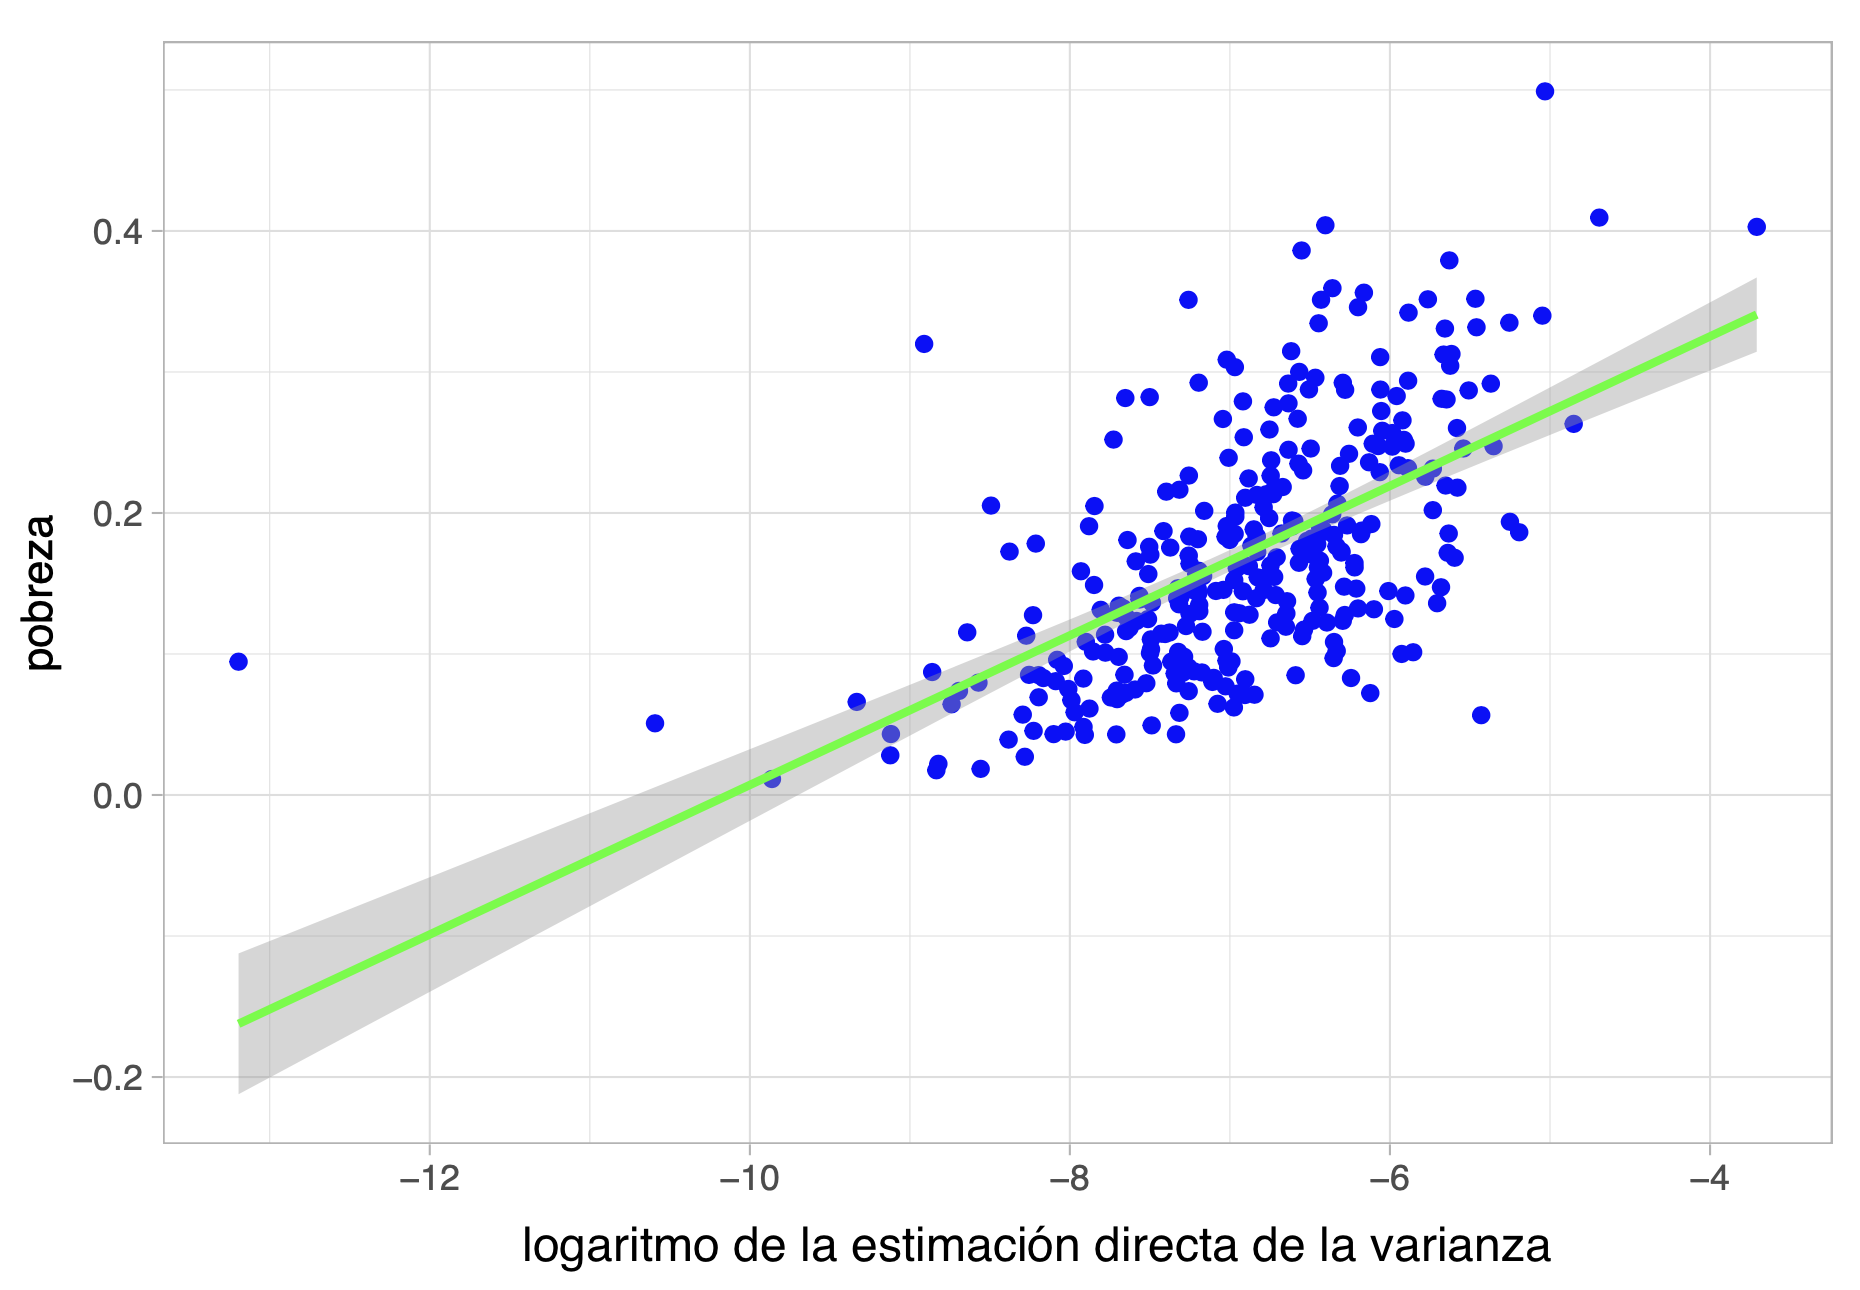
\includegraphics[width=0.5\textwidth,height=\textheight]{Pics/GVFmds.png}
\caption{\emph{Relación entre un estimador de la tasa de pobreza estimada y el logaritmo de la estimación directa de su varianza. Fuente: elaboración propia.}}
\end{figure}

En términos de notación \(Var_{GVF}(\hat{\theta}) = E_m(\widehat{Var}(\hat{\theta}))\) será la varianza suavizada del estimador directo \(\hat{\theta}\). Un aspecto importante en este tipo de modelos es que, en general, no es posible tratar a \(Var(\hat{\theta})\) como un valor fijo puesto que no es estrictamente una función de las covariables auxiliares. Partiendo del hecho de que se tiene acceso a un estimador insesgado de \({Var}(\hat{\theta})\), denotado por \(\widehat{Var}(\hat{\theta})\) se tiene que:

\[
E_{mp}\left(\widehat{Var}(\hat{\theta})\right) =
E_m\left(E_p\left(\widehat{Var}(\hat{\theta})\right)\right) =
E_m({Var}(\hat{\theta})) =
Var_{GVF}(\hat{\theta}) 
\]

La anterior igualdad contiene subscritos \(m\) y \(p\) que hacen referencia a la medida de probabilidad del modelo y del diseño de muestreo, respectivamente. Nótese que aunque el diseño de muestreo induce estimadores de las varianzas que son insesgados, estos tienden a ser inestable cuando el tamaño de muestra es pequeño, que es justo el paradigma dominante en la desagregación de estimaciones. \citet{Rivest_Belmonte_2000} consideran modelos de suavizamiento para la estimación de las varianzas directas definidos de la siguiente manera:

\[
\log(\widehat{Var}(\hat{\theta})) = \mathbf z_d' \boldsymbol \alpha + \varepsilon_d
\]

En donde \(\mathbf z_d\) es un vector de covariables explicativas, \(\boldsymbol \alpha\) es un vector de parámetros que deben ser estimados, \(\varepsilon_d\) son errores aleatorios con media cero y varianza constante, que se asumen idénticamente distribuidos condicionalmente sobre \(\mathbf z_d\). Del anterior modelo, la estimación suavizada de la varianza de muestreo está dada por:

\[
Var_{GVF}(\hat{\theta})  = E_{mp}(\widehat{Var}(\hat{\theta})) = \exp(\mathbf z_d' \boldsymbol \alpha) \cdot \Delta
\]

En donde, \(E_{mp}(\varepsilon_d) = \Delta\). No hay necesidad de especificar una distribución paramétrica para los errores de este modelo. Al utilizar el método de los momentos, se tiene el siguiente estimador insesgado para \(\Delta\):

\[
\hat\Delta = \frac{\sum_{d=1}^D \widehat{Var}(\hat{\theta})}{\sum_{d=1}^D \exp(\mathbf z_d' \boldsymbol \alpha)}
\]

De la misma forma, al utilizar mínimos cuadrados ordinarios, la estimación del coeficiente de parámetros de regresión está dada por la siguiente expresión:

\[
\hat{\boldsymbol \alpha} = \left(\sum_{d=1}^D \mathbf z_d \mathbf z_d' \right)^{-1} \sum_{d=1}^D \mathbf z_d \log(\widehat{Var}(\hat{\theta}))
\]

Por último, el estimador suavizado de la varianza muestral está definido por:

\[
\widehat{Var}_{GVF}(\hat{\theta}) = \exp(\mathbf z_d'\hat{\boldsymbol \alpha})\hat\Delta 
\]

\citet{Rivest_Belmonte_2000} además concluyeron que este estimador no sobrestima ni subestima la varianza suavizada, puesto que el promedio de las estimaciones suavizadas \(\widehat{Var}_{GVF}(\hat{\theta})\) coincide con el promedio de las varianzas directas \(\widehat{{Var}}(\hat{\theta})\). Por tanto:

\[
\frac{\sum_{d=1}^D \widehat{Var}_{GVF}(\hat{\theta}) }{D} = \frac{\sum_{d=1}^D \widehat{{Var}}(\hat{\theta})}{D}
\]

El Instituto de Estadísticas de Canadá (Statcan) utiliza este tipo de modelos para reportar cifras oficiales del mercado de trabajo para 149 áreas censales \citep{statcan2016}. En primer lugar, Statcan hace una exclusión para el ajuste del modelo de aquellas áreas con menos de 10 personas en la fuerza de trabajo (denominador del indicador). De la misma manera todas las áreas con estimador de varianza directa \(\widehat{{Var}}(\hat{\theta})\) igual a cero son excluidas del modelo, puesto que implicaría que no se encontró ningún caso efectivo en el numerador del indicador. Asimismo, la estimación de la varianza directa está basada en el diseño de muestreo complejo, mientras que la estimación de la varianza suavizada está supeditada al siguiente modelo de regresión:
\[
\log(\widehat{Var}(\hat{\theta})) = \mathbf z_d' \boldsymbol \alpha + \varepsilon_d
\]
En donde
\[
\mathbf z_d'=\left(1, \log\left(\frac{N_d^{EIB}}{N_d^{15+}}\right),
\log\left(1-\frac{N_d^{EIB}}{N_d^{15+}}\right),
\log\left(N_d^{15+}\right)\right)'
\]
Con \(N_d^{EIB}\), el número de beneficiarios del seguro de desempleo en el área \(d\) y \(N_d^{15+}\), el número de personas en la fuerza de trabajo. Para las áreas con un tamaño de casos efectivo mayor a 400, para evitar posibles sesgos en las áreas con tamaño de muestra grande, se decidió que la estimación suavizada por GVF fuese igual a la estimación directa; es decir, \(\widehat{Var}_{GVF}(\hat{\theta}) = \widehat{Var}(\hat{\theta})\).

En otra aplicación práctica, \citet{Fuquene_Cristancho_Ospina_Morales_2019} estiman la prevalencia de migrantes internacionales en los municipios de Colombia mediante un modelo de área en el cual utilizan el enfoque GVF, con un modelo que se plantea en términos de una relación log-lineal con el siguiente vector de covariables auxiliares:

\[
\mathbf z_d'=\left(1, \
\hat\theta_d, \
\sqrt{\hat\theta_d}, \
n_d, \
\sqrt{n_d}, \
\sqrt{\hat\theta_d \times n_d} \
\right)'
\]

Asimismo, una de las aplicaciones más citadas se presenta en \citet{III_Herriot_1979}. En este artículo seminal de los modelos de estimación en áreas pequeñas, se relata que el \emph{United States Census Bureau} realizó un censo con una muestra co-censal del 20\% en cada estado para estimar el ingreso percápita. Para estimar este indicador a nivel desagregado se utilizó la estimación directa acompañada con un GVF de varianzas como estimador suavizado. Este modelo tomó los resultados de ocho estados y generalizó para el resto del país. Como resultado de esta modelación, el coeficiente de variación y la varianza se establecieron como una función del tamaño del área.

En la región, \citet{MDSF_CEPAL_2021} utilizaron un modelo GVF para estimar las varianzas de las tasas de pobreza comunal a partir de la CASEN 2020. En este modelo la variable dependiente fue el logaritmo natural de la estimación de la varianza directa de las tasas de pobreza y como covariables se incluyeron al intercepto, a la estimación directa de la tasa de pobreza, al tamaño de muestra comunal, a la interacción entre la tasa de pobreza y el tamaño de muestra, a la raíz cuadrada de la tasa de pobreza, a la raíz cuadrada del tamaño de muestra y, por último, a la raíz cuadrada de la interacción entre la tasa de pobreza y el tamaño de muestra. Las comunas incluidas en la modelación que tuvieron una tasa nula de pobreza, y por consiguiente una estimación nula de la varianza del estimador directo no fueron incluidas en el ajuste del modelo, pero sí se obtuvieron las predicciones de sus varianzas. En el mencionado reporte se muestra esquemas descriptivos que justifican la inclusión de las covariables y las relaciones establecidas en el modelo. Además, el factor de ajuste \(\hat\Delta\) estuvo cercano a 1.2 en todas las series estudiadas.

\hypertarget{consideraciones-adicionales-sobre-la-estimaciuxf3n-de-la-varianza-de-los-estimadores-de-muestreo}{%
\section{Consideraciones adicionales sobre la estimación de la varianza de los estimadores de muestreo}\label{consideraciones-adicionales-sobre-la-estimaciuxf3n-de-la-varianza-de-los-estimadores-de-muestreo}}

En la práctica del muestreo, existen algunos paradigmas que inducen la planeación y diseño de las encuestas. En esta sección se muestran ejemplos y contra-ejemplos que permiten ilustrar algunas mitos en la estimación del error de muestreo de las encuestas de hogares. Para esto, consideremos la varianza del esimador HT, dada a continuación:

\[
Var(\hat{t}_{y, \pi})=
\sum_{k\in U}\sum_{l\in U} \Delta_{kl}\frac{y_k}{\pi_k}\frac{y_l}{\pi_l}
\]

En donde \(\Delta_{kl} = (\pi_{kl}-\pi_k\pi_l)\) y \(\pi_{kl}\) denota la probabilidad de inclusión conjunta de los elementos \(k\) y \(l\) pertenezcan a la muestra \(s\). Bajo diseños de muestreo de tamaño fijo, existen dos estimadores insesgados para esta varianza, el primero originalmente propuesto por \citet{HT} y dado por

\[
\widehat{Var}_1(\hat{t}_{y, \pi})=
\sum_{k\in s}\sum_{l\in s} \frac{\Delta_{kl}}{\pi_{kl}}\frac{y_k}{\pi_k}\frac{y_l}{\pi_l}
\]

El segundo estimador propuesto por \citet{Sen} y \citet{YG}, está dado por la siguiente expresión:

\[
\widehat{Var}_2(\hat{t}_{y, \pi})=-\frac{1}{2}
\sum_{k\in s}\sum_{l\in s} \frac{\Delta_{kl}}{\pi_{kl}}\left(\frac{y_k}{\pi_k}-\frac{y_l}{\pi_l}\right)^2
\]

\hypertarget{estimaciones-negativas-de-varianza}{%
\subsection{Estimaciones negativas de varianza}\label{estimaciones-negativas-de-varianza}}

La idea de que no pueden existir estimaciones negativas de la varianza se ha instalado como un razonamiento bastante lógico e intuitivo: dado que la varianza es un parámetro positivo, entonces no puede ser estimada con cantidades negativas. Sin embargo, en la inferencia basada en el diseño de muestreo, sí es posible obtener estimativas negativas de varianza para algunas estructuras poblacionales particulares y es por esto que se requiere una experiencia mayor por parte del equipo de muestreo, que debe conocer bajo qué condiciones se podría presentar esta situación para evadirla.

Nótese que se debe diferenciar entre estimador (que es una función de variables aleatorias) y parámetro (que es un valor real desconocido). En efecto, para la varianza del estimador HT (parámetro desconocido y siempre positivo) hay estimadores (función de variables aleatorias) que pueden arrojar estimaciones negativas. Es posible que las estimaciones de la varianza arrojen resultados negativos, que no pueden ser utilizados ni interpretados. Considere el siguiente diseño de muestreo de tamaño fijo e igual a \(n=2\), el cual induce seis posibles muestras.

\begin{longtable}[]{@{}rrrrrr@{}}
\toprule()
\(s\) & \(I_1\) & \(I_2\) & \(I_3\) & \(I_4\) & \(p(s)\) \\
\midrule()
\endhead
\(s_1\) & 1 & 1 & 0 & 0 & 0.31 \\
\(s_2\) & 1 & 0 & 1 & 0 & 0.20 \\
\(s_3\) & 1 & 0 & 0 & 1 & 0.14 \\
\(s_4\) & 0 & 1 & 1 & 0 & 0.03 \\
\(s_5\) & 0 & 1 & 0 & 1 & 0.01 \\
\(s_6\) & 0 & 0 & 1 & 1 & 0.31 \\
\bottomrule()
\end{longtable}

En el anterior ejemplo, la probabilidad de obtener una muestra compuesta por los dos primeros elementos se fijó en 0.31; mientras que la probabilidad de obtener una muestra compuesta por el primer y el tercer elemento se fijó en 0.20 y así sucesivamente. Para esta configuración se obtienen las estimaciones puntuales para cada una de las seis posibles muestras, así como las dos posibles estimaciones de la varianza. Nótese que para ambos escenarios existen estimaciones negativas.

\begin{longtable}[]{@{}
  >{\raggedleft\arraybackslash}p{(\columnwidth - 16\tabcolsep) * \real{0.0690}}
  >{\raggedleft\arraybackslash}p{(\columnwidth - 16\tabcolsep) * \real{0.0690}}
  >{\raggedleft\arraybackslash}p{(\columnwidth - 16\tabcolsep) * \real{0.0690}}
  >{\raggedleft\arraybackslash}p{(\columnwidth - 16\tabcolsep) * \real{0.0690}}
  >{\raggedleft\arraybackslash}p{(\columnwidth - 16\tabcolsep) * \real{0.0690}}
  >{\raggedleft\arraybackslash}p{(\columnwidth - 16\tabcolsep) * \real{0.0862}}
  >{\raggedleft\arraybackslash}p{(\columnwidth - 16\tabcolsep) * \real{0.1552}}
  >{\raggedleft\arraybackslash}p{(\columnwidth - 16\tabcolsep) * \real{0.2069}}
  >{\raggedleft\arraybackslash}p{(\columnwidth - 16\tabcolsep) * \real{0.2069}}@{}}
\toprule()
\begin{minipage}[b]{\linewidth}\raggedleft
\(s\)
\end{minipage} & \begin{minipage}[b]{\linewidth}\raggedleft
\(I_1\)
\end{minipage} & \begin{minipage}[b]{\linewidth}\raggedleft
\(I_2\)
\end{minipage} & \begin{minipage}[b]{\linewidth}\raggedleft
\(I_3\)
\end{minipage} & \begin{minipage}[b]{\linewidth}\raggedleft
\(I_4\)
\end{minipage} & \begin{minipage}[b]{\linewidth}\raggedleft
\(p(s)\)
\end{minipage} & \begin{minipage}[b]{\linewidth}\raggedleft
\(\hat{t}_{y, \pi}\)
\end{minipage} & \begin{minipage}[b]{\linewidth}\raggedleft
\(\widehat{Var}_1(\hat{t}_{y, \pi})\)
\end{minipage} & \begin{minipage}[b]{\linewidth}\raggedleft
\(\widehat{Var}_2(\hat{t}_{y, \pi})\)
\end{minipage} \\
\midrule()
\endhead
\(s_1\) & 1 & 1 & 0 & 0 & 0.31 & 9.560440 & 38.099984 & -0.9287681 \\
\(s_2\) & 1 & 0 & 1 & 0 & 0.20 & 5.883191 & -4.744190 & 2.4710422 \\
\(s_3\) & 1 & 0 & 0 & 1 & 0.14 & 4.933110 & -3.680428 & 8.6463858 \\
\(s_4\) & 0 & 1 & 1 & 0 & 0.03 & 7.751323 & -100.252974 & 71.6674365 \\
\(s_5\) & 0 & 1 & 0 & 1 & 0.01 & 6.801242 & -165.715154 & 323.3238494 \\
\(s_6\) & 0 & 0 & 1 & 1 & 0.31 & 3.123994 & 3.426730 & -0.1793659 \\
\bottomrule()
\end{longtable}

A pesar de los resultados negativos para las varianzas, tanto el estimador del total como los dos estimadores de su varianza siguen siendo insesgados. En efecto al multiplicar la estimación puntual por la probabilidad del diseño de muestreo se obtienen los valores poblacionales. La varianza del estimador HT para este diseño en particular es 6.744442, la cual corresponde con la esperanza de ambos estimadores de varianza. Para evitar estas estimativas negativas, \citet{Gutierrez_2016} afirma que es necesario garantizar que la covarianza (\(\Delta_{kl}\)) sea negativa para cada par de elementos en la población (\(k \neq l\)), lo cual no sucede con este esquema de muestreo, puesto que:

\[
\Delta_{kl} =
\begin{bmatrix}
0.2275  & 0.0825  & -0.1510 & -0.1590 \\
0.0825  & 0.2275  & -0.1590 & -0.1510 \\
-0.1510 & -0.1590 & 0.2484  & 0.0616 \\
-0.1590 & -0.1510 & 0.0616  &  0.2484
\end{bmatrix}
\]

\hypertarget{disminuciuxf3n-de-la-varianza-ante-el-aumento-del-tamauxf1o-de-muestra}{%
\subsection{Disminución de la varianza ante el aumento del tamaño de muestra}\label{disminuciuxf3n-de-la-varianza-ante-el-aumento-del-tamauxf1o-de-muestra}}

Por otro lado, la idea de que al aumentar el tamaño de la muestra debería disminuir la varianza deriva de la lógica intuitiva en donde el error de muestreo no debería existir si se realiza una medición completa de la población. Sin embargo, aunque esto es lo que por lo general ocurre, hay algunas excepciones. Luego, para algunas estrategias de muestreo es posible encontrar que existen situaciones en donde el tamaño de muestra crece, y con él la varianza del estimador. En esta sección se mostrará un ejemplo en donde sucede exactamente eso.

Para poder mostrar este hecho, vamos a utilizar un ejemplo reducido. Supongamos una población de \(N = 3\) elementos \(U=\{1, 2, 3\}\) y comparemos dos diseños de muestreo, el primero con un tamaño de muestra fijo de \(n=1\) y el segundo con un tamaño de muestra fijo de \(n=2\). En ambos casos la variable de interés es dicotómica que denota la presencia o ausencia del fenómeno en los individuos de la población. En el primer caso, el diseño de muestreo de tamaño de muestra \(n=1\) es el siguiente:

\begin{longtable}[]{@{}rrrrr@{}}
\toprule()
\(s\) & \(I_1\) & \(I_2\) & \(I_3\) & \(p(s)\) \\
\midrule()
\endhead
\(s_1\) & 1 & 0 & 0 & 0.5 \\
\(s_2\) & 0 & 1 & 0 & 0.1 \\
\(s_3\) & 0 & 0 & 1 & 0.4 \\
\bottomrule()
\end{longtable}

En este esquema de muestreo, la varianza del estimador de Horvitz-Thompson es igual a \(Var(\hat t_{y, \pi}) = 1.5\). Sin embargo, en un segundo caso, considere el siguiente diseño de muestreo de tamaño de muestra \(n=2\):

\begin{longtable}[]{@{}rrrrr@{}}
\toprule()
\(s\) & \(I_1\) & \(I_2\) & \(I_3\) & \(p(s)\) \\
\midrule()
\endhead
\(s_1\) & 1 & 1 & 0 & 0.7 \\
\(s_2\) & 1 & 0 & 1 & 0.2 \\
\(s_3\) & 0 & 1 & 1 & 0.1 \\
\bottomrule()
\end{longtable}

Nótese que en este esquema de muestreo, la varianza del estimador de Horvitz-Thompson es igual a \(Var(\hat t_{y, \pi}) = 2.3\). Por tanto, no es exacto afirmar que siempre que un diseño de muestreo contemple un tamaño de muestra más grande se tendrá obligatoriamente una reducción de la varianza.

\hypertarget{representatividad-y-ausencia-de-respuesta}{%
\chapter{Representatividad y ausencia de respuesta}\label{representatividad-y-ausencia-de-respuesta}}

El problema de la ausencia de respuesta es una faceta normal, aunque no deseable, en el desarrollo de una encuesta. Todas las encuestas de hogares sufren del fenómeno de la ausencia de respuesta ya sea de hogares completos, de personas dentro de los hogares, o en en algunas de las variables de interés dentro de los cuestionarios. En algunas ocasiones y aún después de un diseño cuidadoso y una planificación logística exhaustiva, esta problemática puede ser tan grande que los resultados de la encuesta pueden quedar en entredicho. Por esta razón, este problema debe ser considerado en la planificación y el diseño de todos los levantamientos de información a través de encuestas y se debe contemplar varios ajustes que prevean las consecuencias de este fenómeno. Es por esto que en los capítulos anteriores se abordó el tema del ajuste de subcobertura, que garantiza que el tamaño de muestra efectivo sea el adecuado para realizar un inferencia precisa. De otra forma, si el diseño de la encuesta no tiene en cuenta estos ajustes, el tamaño de muestra final se verá reducido puesto que muchos hogares no contestarán algunas preguntas del cuestionarios, y en algunos casos, muchos hogares no contestarán la totalidad del cuestionario.

Existe un consenso general de que la ausencia de respuesta puede perjudicar severamente la calidad de las estadísticas calculadas y publicadas en una encuesta. \citet{Lohr_2019} afirma que la mayoría de encuestas tienen cierta ausencia de respuesta residual, aún después de un diseño cuidadoso y un seguimiento de la ausencia de respuesta y establece que existen varios tipos de mecanismos de ausencia de respuesta.

\begin{enumerate}
\def\labelenumi{\arabic{enumi}.}
\tightlist
\item
  Se define la ausencia de respuesta ignorable cuando la probabilidad de que un individuo responda no depende de la característica de interés. Nótese que el adjetivo ignorable hace referencia a que un modelo puede explicar el mecanismo de ausencia de respuesta y que ésta se puede ignorar después de que el modelo la toma en cuenta.
\item
  Por otra parte, la ausencia de respuesta se dice no ignorable cuando la probabilidad de que un individuo responda depende de la característica de interés. Por ejemplo, si en una encuesta de fuerza laboral, se desea estimar el número de personas empleadas o desempleadas, la ausencia de respuesta es no ignorable cuando depende de la clasificación laboral del individuo.
\end{enumerate}

En términos de literatura, el fenómeno de la ausencia de respuesta y sus repercusiones negativas sobre la calidad de las estimaciones ha sido ampliamente estudiado. Por ejemplo, \citet[capítulo 9]{Lumley_2010} hace un análisis detallado con la ausencia de respuesta individual, en donde existen datos parciales para un respondiente, considerando un enfoque que está basado en el diseño de muestreo al ajustar los pesos muestrales. \citet[capítulo 5]{Fuller} cita algunas técnicas de imputación para el tratamiento de la ausencia de respuesta y conjuga modelos probabilísticos junto con los pesos del diseño de muestreo para mitigar los efectos de este problema. \citet{Sar1} considera un enfoque asistido por modelos, en donde toma conjuntos balanceados para lograr mayor representatividad de las estimaciones. De la misma forma, \citet{Sar2} propone un conjunto de indicadores para juzgar la efectividad de la información auxiliar utilizada para controlar el sesgo generado por la ausencia de respuesta.

\hypertarget{el-concepto-de-representatividad}{%
\section{El concepto de representatividad}\label{el-concepto-de-representatividad}}

El concepto de representatividad se utiliza a menudo en la investigación
de encuestas, pero por lo general no está claro qué significa. En particular Kruskal y Mosteller presentan una amplia descripción
de lo que se supone que significa el adjetivo representativo \citep[\citet{KruskalMosteller2}, \citet{KruskalMosteller3}, \citet{KruskalMosteller4}]{KruskalMosteller1}. El concepto de muestra representativa no está del todo estandarizado; \citet{Bethlehem_Cobben_Schouten_2009} menciona que algunos de estos conceptos son muy vagos e imprecisos; por ejemplo:

\begin{itemize}
\tightlist
\item
  Reconocimiento general de los datos.
\item
  Ausencia de fuerzas selectivas en la muestra.
\item
  Una muestra que sea una miniatura de la población.
\item
  Una muestra que contenga casos típicos o ideales.
\item
  Cobertura suficiente de la población,
\item
  Que permite una buena estimación,
\item
  Suficientemente bueno para un propósito particular.
\end{itemize}

En términos de notación, supongamos que se selecciona una muestra probabilística \(s\) de tamaño \(n\) sin reemplazo de una población finita \(U\) de tamaño \(N\). La muestra puede verse como un vector de \(N\) indicadores \(s=(I_{1},I_{2},\ldots,I_{N})\), donde el indicador \(I_{k}=1\) si se selecciona el elemento \(k\) en la muestra, y \(I_{k}=0\) en caso contrario (\(k=1,2,\ldots,N\)). El fenómeno de la ausencia de respuesta se modela por medio de las probabilidades de respuesta. Para esto, se supone que cada elemento \(k\) en la población tiene una cierta probabilidad desconocida \(\phi_{k}\) de responder cuando se selecciona en la muestra. La respuesta a la encuesta se puede representar mediante el vector de indicadores \(D=(D_{1},D_{2},\ldots,D_{N})\), donde \(D_{k}=1\) si el elemento \(k\) fue seleccionado en la muestra \((I_{k}=1)\) y respondió. De lo contrario, \(D_{k}=0\). Por ende, se deduce que

\[
\phi_{k}=P\left(D_{k}=1\mid I_{k}=1\right)
\]

Para poder definir un indicador de representatividad, el concepto
de representatividad que mejor se acomoda se define como \emph{la ausencia de fuerzas selectivas}. Está claro que no existen fuerzas selectivas si todas las probabilidades de respuesta son uniformes. Esta observación forma la base de la primera definición de representatividad.

La respuesta a una encuesta se denomina \emph{fuertemente representativa} con
respecto a la muestra, si las probabilidades de respuesta de todos
los elementos de la población son iguales y si la respuesta de un
elemento es independiente de la respuesta de todos los demás elementos.
En otras palabras:

\[
\phi_{k} = P\left(D_{k}=1\mid I_{k}=1\right) =  \phi  \ \ \ \ \ \ \ \ \ \ k=1,2,\ldots,N
\]

Se debe tener en cuenta que la representatividad fuerte se garantiza cuando el mecanismo de datos faltantes es MCAR para cada variable objetivo en el estudio. En este caso, la falta de respuesta no provoca que los estimadores estén sesgados. Esta es una definición atractiva, pero no es muy útil ya que en la práctica no es posible comparar las probabilidades de respuesta individual.

Por otro lado, suponga que hay una variable auxiliar categórica \(X\) que tiene \(H\)
categorías y divide la población en \(H\) estratos (subpoblaciones).
El número de elementos en el estrato \(h\) se denota por \(N_{h}\),
para \(h=1,2,\ldots,H\). Se asume que esta variable ha sido medida
en la encuesta y que su valor está disponible para cada encuestado
y no encuestado. La probabilidad de respuesta del elemento \(k\) en
el estrato \(h\) está definida por \(\phi_{hk}\).

La respuesta a una encuesta se denomina \emph{débilmente representativa}
con respecto a la muestra para la variable auxiliar \(X\) si la probabilidad
de respuesta promedio es la misma en cada estrato, es decir,

\[
\bar{\phi}_{h} =  
\frac{1}{N_{h}}\sum_{k=1}^{N_{h}}\phi_{hk} =
\phi \ \ \ \ \ \ \ \ \ \  h=1,2,\ldots,H
\]

La representatividad débil significa que no es posible distinguir
a los encuestados de los no encuestados simplemente usando información
con respecto a \(X\). Si la respuesta es débilmente representativa con respecto a muchas variables auxiliares \(X\), existirán relaciones fuertes entre las variables objetivo y las variables auxiliares. Nótese que es posible estimar las medias de las probabilidades de respuesta en los estratos y, por lo tanto, se puede comprobar en la práctica el supuesto de representatividad débil.

\hypertarget{indicadores-de-representatividad}{%
\section{Indicadores de representatividad}\label{indicadores-de-representatividad}}

Como se mencionó anteriormente, la mayoría de las encuestas adolecen de falta de respuesta y este fenómeno puede afectar seriamente la calidad de
los resultados de una encuesta. De hecho, las estimaciones de las características de la población estarán sesgadas si, debido a la falta de respuesta, algunos grupos de la población quedan sobre-representados o sub-representados; el problema se agrava cuando estos grupos
se comportan de manera diferente con respecto a las variables de la
encuesta. En referencia a la ausencia de respuesta de unidad, en general los INE de la región a menudo usan la tasa de respuesta de la encuesta como un indicador de la calidad de la encuesta.

Dado que una tasa de respuesta baja no implica necesariamente que la precisión de las estimaciones de la encuesta sea deficiente, centrarse solo en la tasa de respuesta como indicador de la calidad de la encuesta puede ser engañoso. Por ejemplo, \citet{Bethlehem_Cobben_Schouten_2009} ilustran esta situación con un ejemplo de la encuesta holandesa POLS en 1998 (Encuesta Integrada de Condiciones de Vida de los Hogares). Después de un mes de trabajo de campo, la tasa de respuesta fue del 47,2\%, mientras que después del período completo de dos meses, la tasa había aumentado al 59,7\%. El modo de recolección de datos en el primer mes fue CAPI (entrevista
personal asistida por computadora). Los que no respondieron fueron
contactados en el segundo mes con CATI (Entrevista Telefónica Asistida
por Computadora) si tenían un teléfono fijo en la lista. El segundo mes de trabajo de campo aumentó la respuesta en un 12,5\%. Sin embargo, esto no resultó en mejores estimaciones puesto que el sesgo de los estimadores aumentó a partir del segundo mes, dado que las personas que habían reportado un número telefónico diferían de las que no reportaron este contacto.

Adicional a la tasa de no respuesta, se necesitan indicadores
de calidad de la encuesta que proporcionen más información sobre el
posible riesgo de estimadores sesgados.

\citet{Shlomo_Skinner_Schouten_2012} estudian el uso de los \emph{indicadores de representatividad} (Indicadores \(R\)) que permiten conocer qué tanto la muestra de respondientes efectivos representa a la población y cómo la composición de la respuesta en la muestra diferiría de la composición de la población finita. Estos indicadores han probado ser una guía importante para determinar en qué medida el sesgo causado por la ausencia de respuesta afecta la encuesta. De hecho, en Europa el proyecto RISQ (\emph{Representativity Indicators for Survey Quality}) está basado en este enfoque y pretende desarrollar y probar indicadores R en varias encuestas de interés. Los países que participan en este proyecto Holanda, Noruega y Eslovenia, en conjunto con las universidad de Southampton (Reino Unido) y la Universidad de Lovaina (Bélgica).

Los indicadores \(R\) miden hasta qué punto la composición de
la respuesta a una encuesta se desvía de la muestra original. Si todas las probabilidades de respuesta son iguales, la respuesta
es fuertemente representativa y no habrá diferencias sistemáticas
entre la composición de la respuesta y la muestra. Por el contrario, si las probabilidades de respuesta no son iguales, es importante
establecer en qué medida se ve afectada la composición de la respuesta. Esto se logra mediante la definición de una función de distancia
que mide en qué medida las probabilidades de respuesta individuales
difieren de la probabilidad de respuesta media.

Supongamos que se conocen las probabilidades de respuesta individual
\(\phi_{1},\phi_{2},\ldots,\phi_{N}\) de todos los elementos de la población.
Entonces la desviación estándar es

\[
S\left(\phi\right)  =  \sqrt{\frac{1}{N-1}\sum_{k=1}^{N}\left(\phi_{k}-\bar{\phi}\right)^{2}}
\]

Nótese que \(S\left(\phi\right)=0\) si todas las probabilidades de respuesta
son iguales y el valor de \(S\left(\phi\right)\) será mayor a medida
que haya más variación en los valores de las probabilidades de respuesta. Además, el valor máximo de \(S\left(\phi\right)\) es igual a 0.5. Por ende, el indicador \(R\) se define como:

\[
R\left(\phi\right)=1-2\,S\left(\phi\right)
\]

Este indicador asume valores en el intervalo \(\left[0,1\right]\). De esta manera, un valor de uno implica una fuerte representatividad. Cuanto menor es su valor, más se desvía la composición de respuesta
de la composición de la muestra. En general, los valores de las probabilidades de respuesta individuales se desconocen en la práctica. Este problema se resuelve estimando las probabilidades de respuesta. Esto se puede lograr si se dispone de información auxiliar adecuada; es decir, de variables que se han medido tanto para los encuestados como para los no encuestados. Para estimar estas probabilidades es posible utilizar varias técnicas, por ejemplo, modelos logísticos o probit, árboles de clasificación, entre otras.

Al suponer que \(\hat{\phi}_{1},\hat{\phi}_{2},\ldots,\hat{\phi}_{n}\) son
las probabilidades de respuesta estimadas para las unidades en la muestra.
Entonces, la probabilidad de respuesta media se puede estimar mediante

\[
\hat{\bar{\phi}}  =  \frac{1}{N}\sum_{k=1}^{n}\frac{\hat{\phi}_{k}}{\pi_{k}}
\]

y

\[
\hat{R}\left(\phi\right)  =  1-2\sqrt{\frac{1}{N-1}\sum_{k=1}^{n}\frac{\left(\hat{\phi}_{k}-\hat{\bar{\phi}}\right)^{2}}{\pi_{k}}}
\]

Nótese que el indicador \(R\) mide la desviación de la representatividad débil y no de la representatividad fuerte. Por ende, este enfoque no es capaz de detectar y cuantificar las diferencias
entre las probabilidades de respuesta individual dentro de las clases obtenidas al cruzar las variables auxiliares. Suponiendo que las clases están definidas por una variable auxiliar \(X\) que tiene \(H\) categorías. Sea \(N_{h}\) el tamaño de la clase \(h\) y sea \(\bar{\phi}_{h}\) la media poblacional de las probabilidades de respuesta en el estrato \(h\). Si se utiliza un modelo estándar como la regresión logística, el indicador \(R\) se calcula como:

\[
R_{x}\left(\phi\right)  =  1-2\sqrt{\frac{1}{n-1}\sum_{h=1}^{H}N_{h}\left(\bar{\phi}_{h}-\bar{\phi}\right)^{2}}
\]

En este caso, \(R_{x}\left(\phi\right)\) mide la variación de las probabilidades de respuesta entre clases \(X\). Si se supone que la variación dentro de la clase es cero en todas las clases, entonces \(R_{x}\left(\phi\right) = R\left(\phi\right)\).

\citet{Bethlehem_Cobben_Schouten_2009} mencionan que de julio a diciembre de 2005, Statistics Netherlands realizó un seguimiento a gran escala entre los no encuestados en la Encuesta de Población Activa (EPA) de Holanda. En el estudio, se abordó a dos muestras de personas que no respondieron en la EPA utilizando, por un lado, el enfoque de devolución de llamada con el cuestionario completo de la EPA y, por el otro lado, el enfoque de preguntas básicas con un cuestionario muy corto. Se usó CATI en el enfoque de devolución de llamada, y el enfoque de preguntas básicas se utilizó un diseño de recolección mixto que involucró cuestionarios \emph{online} y recolección presencial con papel y CAPI. Los indicadores R se estimaron utilizando modelos de regresión logística que incluían una gran cantidad de variables explicativas que medían características demográficas, geográficas y socioeconómicas en los hogares. Los resultados de este estudio se dan a continuación:

\begin{enumerate}
\def\labelenumi{\arabic{enumi}.}
\tightlist
\item
  Se reportó que el valor del indicador \(R\) para la respuesta inicial de la EPA es igual a 0.8, que es menor que el valor ideal de 1. Entonces, esta respuesta no es fuertemente representativa. La aplicación del enfoque de devolución de llamada aumentó la
  tasa de respuesta del 62.2\% al 76.9\%. Luego de esto, el valor del indicador \(R\) aumentó de 0.8 a 0.85. Como los intervalos de confianza no se superponían, hubo indicios de que la respuesta adicional mejoró la composición del conjunto de datos.
\item
  La aplicación del enfoque de preguntas básicas dio como resultado
  una conclusión diferente. Aunque la tasa de respuesta aumentó del 62.2\% al 75.6\%, el valor del indicador \(R\) disminuyó de 0.80 a 0.78. Los intervalos para la EPA inicial y la EPA con preguntas básicas, se superpusieron. Por lo tanto, aparentemente, el enfoque de preguntas básicas no mejoró la composición del conjunto de datos.
\end{enumerate}

Este último enfoque no es novedoso y agudiza el contraste entre respondientes y no respondientes. Dado que las probabilidades de respuesta estimadas se utilizan para calcular
el indicador \(R\) y esta estimación se basa en un modelo lineal que utiliza un conjunto de variables auxiliares como variables explicativas.

La dependencia del indicador \(R\) del conjunto de variables auxiliares utilizadas tiene implicaciones para comparar diferentes conjuntos de datos (por ejemplo, en el tiempo o en dominios). Un enfoque apropiado podría ser fijar el conjunto de variables auxiliares de antemano y mantenerlas iguales para todos los conjuntos de datos. Para ello, debe elegirse el máximo posible de variables. Por otro lado, debido al sobreajuste, el error estándar (estimado) puede verse
afectado, pero las probabilidades de respuesta estimadas no serán sesgadas.

Otro enfoque que se recomienda, es intentar encontrar el mejor modelo para cada conjunto de datos utilizando técnicas de selección de modelos. Esto hace que los modelos dependan del tamaño de la muestra: cuanto
mayor sea la muestra, más variables del modelo tendrán una contribución significativa. Las muestras pequeñas simplemente no permiten una estimación adecuada de las probabilidades de respuesta y conducirán a una visión más optimista de la representatividad.

Con esta metodología es posible determinar si la composición de la muestra de respondientes efectivos difiere o no de la de la muestra inicial. Los resultados de este proceso de seguimiento pueden ayudar a sustentar
la decisión de iniciar esfuerzos adicionales para obtener datos para grupos específicos de la población objetivo; este enfoque también puede resultar útil para evaluar si volver a abordar una muestra de personas que no respondieron sería una buena estrategia para acotar el sesgo, o si con un enfoque de preguntas básicas sería suficiente.

El uso de esta metodología durante la fase de recolección de datos podría revelar que la composición de los datos observados se está desviando cada vez más de la estructura poblacional esperada. Esto podría llevar a la decisión de enfocar el resto del proceso de recolección en los grupos que están subrepresentados. Estos cambios en medio de la encuesta se conocen en la literatura especializada como \emph{diseños receptivos}. Otra forma de utilizar el indicador \(R\) para controlar el proceso de la encuesta es analizar la representatividad de una versión anterior de la encuesta. Los resultados de dicho análisis pueden proporcionar información para implementar una estrategia mejorada de recopilación de datos para una nueva versión de la encuesta.

\hypertarget{clasificaciuxf3n-de-la-ausencia-de-respuesta}{%
\section{Clasificación de la ausencia de respuesta}\label{clasificaciuxf3n-de-la-ausencia-de-respuesta}}

Por otra parte, \citet{Lund} aclaran que existe una gran cantidad de literatura acerca de la ausencia de respuesta y muchos artículos recientes. Esta literatura examina dos aspectos diferentes pero complementarios en el ejercicio de una encuesta: la prevención de la ausencia de respuesta (antes de que ocurra) y las técnicas de estimación necesarias para tener en cuenta la ausencia de respuesta de manera apropiada en el proceso de inferencia. Esta segunda actividad se conoce con el nombre de ajuste para la ausencia de respuesta. \citet{LR2002} establecen tres tipos de ausencia de respuesta.

La ausencia de respuesta completamente aleatoria (MCAR - \emph{missing completely at random}) se presenta cuando la probabilidad de que un individuo responda no depende de la característica de interés, ni de alguna otra covariable auxiliar. Por ejemplo, si la ausencia de respuesta en una encuesta laboral, no depende del estado actual de empleo del respondiente, ni de alguna característica auxiliar. De esta forma, la ausencia de respuesta está dispersa de manera uniforme sobre toda la población.

Es decir que, cuando el investigador produzca estadísticas descriptivas sobre las personas que respondieron la encuesta, ese porcentaje de personas sea muy similar y tenga un comportamiento uniforme sobre todas las posibles covariables que afecten al individuo. El gráfico \ref{fig:mcar} podría mostrar algunos indicios de que el patrón de ausencia de respuesta podría ser MCAR puesto que el porcentaje de respuesta es similar en las variables auxiliares.

\begin{figure}
\centering
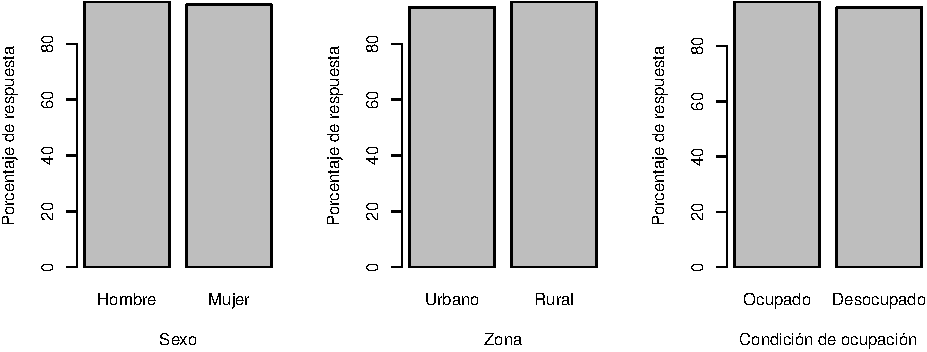
\includegraphics{12Ausencia_files/figure-latex/mcar-1.pdf}
\caption{\label{fig:mcar}Patrón de respuesta MCAR}
\end{figure}

La ausencia de respuesta aleatoria (MAR - \emph{missing at random}) se establece cuando la probabilidad de que un individuo responda depende de algunas covariables auxiliares, pero no depende de la característica de interés. Por ejemplo, en una encuesta de fuerza laboral, la ausencia de respuesta puede depender de la edad del respondientes, o del sexo, o incluso del nivel económico del individuo, pero no depende de su clasificación laboral. El gráfico \ref{fig:mar} muestra que el patrón de ausencia de respuesta podría ser MAR puesto que el sexo y la zona del respondiente están influenciando el porcentaje de respuesta, aunque no el estado de ocupación.

\begin{figure}
\centering
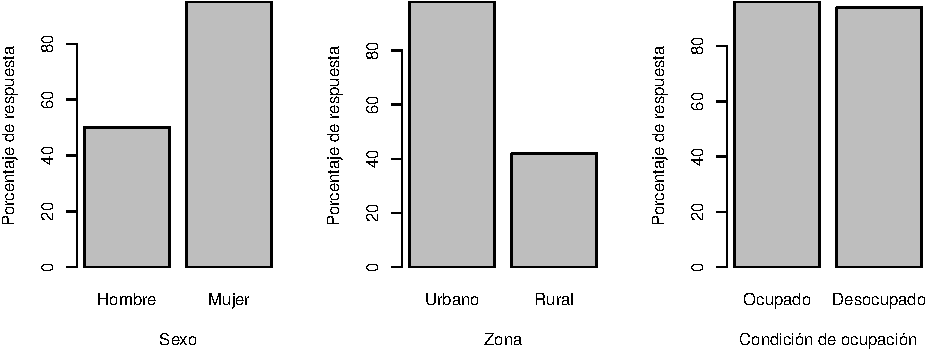
\includegraphics{12Ausencia_files/figure-latex/mar-1.pdf}
\caption{\label{fig:mar}Patrón de respuesta MAR}
\end{figure}

Por último, la ausencia de respuesta no aleatoria (NMAR - \emph{not missing at random}) se presenta cuando la ausencia de respuesta depende de la característica de interés. El gráfico \ref{fig:nmar} muestra indicios de que el patrón de respuesta es NMAR, puesto que la condición de ocupación es la que influencia el porcentaje de respuesta; esto es contraproducente porque no existirá una forma simple de mitigar el sesgo generado por esta clase de ausencia de respuesta.

\begin{figure}
\centering
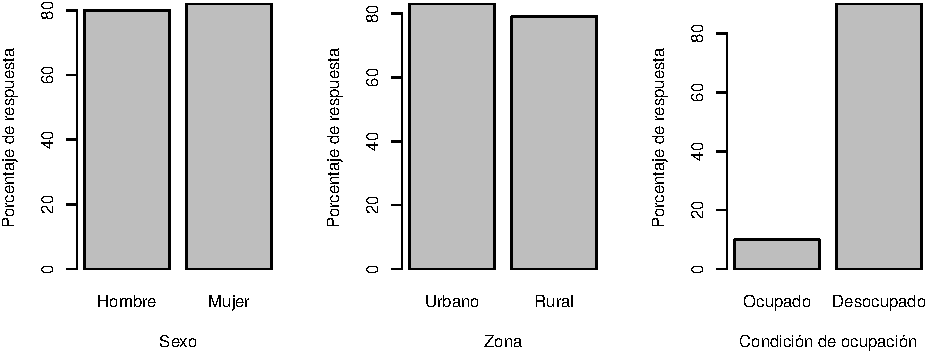
\includegraphics{12Ausencia_files/figure-latex/nmar-1.pdf}
\caption{\label{fig:nmar}Patrón de respuesta MNAR}
\end{figure}

\hypertarget{ausencia-de-respuesta-de-registro-y-de-unidad}{%
\section{Ausencia de respuesta de registro y de unidad}\label{ausencia-de-respuesta-de-registro-y-de-unidad}}

Nótese que a pesar de que se hayan tomado las medidas de ajuste necesarias en el diseño de la encuesta, cuando ya ha terminado el proceso de recolección de información, se debe lidiar con la ausencia de respuesta para evitar sesgos y aumentar la precisión de los estimadores en la encuesta. La literatura especializada examina dos metodologías diferentes pero complementarias en el ejercicio de una encuesta: la prevención de la ausencia de respuesta (antes de que ocurra) y las técnicas de estimación necesarias para tener en cuenta la ausencia de respuesta de manera apropiada en el proceso de inferencia, después de la recolección de los datos.

Si el mecanismo de ausencia de respuesta se asume MCAR, es posible contemplar en el proceso de inferencia únicamente a aquellas unidades que tienen registros completos y eliminar de la base de datos a aquellas unidades que no contestaron (\emph{list-wise deletion}). A pesar de que este tipo de análisis es simple, para evitar subestimaciones de los parámetros de interés, se debe realizar un ajuste de los factores de expansión inducidos por el diseño muestral, que originalmente fue planeado con un tamaño de muestra más grande que el efectivo. De esta forma, es posible suponer que la muestra de respondientes corresponde a una submuestra completamente aleatoria de la población y utilizar los principios de los diseños en dos fases. \citet[capítulo 11]{Heeringa_West_Berglund_2010} afirman que este tipo de análisis, además de inducir posibles sesgos si el supuesto MCAR no se cumple, reduce la eficiencia de la inferencia debido al decremento del tamaño de muestra efectivo. Por lo tanto, en la mayoría de encuestas, este supuesto no se asume y se realiza un ajuste adicional, después de que ha ocurrido la ausencia de respuesta.

En general se puede afirmar que existen dos tipos de ausencia de respuesta: la primera, debido a la falta de respuesta de una unidad de observación (ausencia de respuesta de unidad), y la segunda debido a la falta de respuesta de una unidad en algunas variables de interés (ausencia de respuesta por registro). Es por esto que \citet[sección 15.5]{Sarndal_Swensson_Wretman_2003} afirman que las principales técnicas para tratar la ausencia de respuesta son el ajuste a los pesos de muestreo y la imputación. El ajuste por ponderación implica aumentar los pesos aplicados en la estimación de los valores y de los encuestados para compensar los valores que se pierden debido a la ausencia de respuesta, mientras que la imputación implica la sustitución de los valores faltantes por valores artificiales.

La ausencia de respuesta tiene una repercusión evidente en la base de datos de la encuesta. Por ejemplo, en la base de datos inicial puede faltar toda la información de una unidad de observación; esto suele suceder porque el encuestador no pudo establecer contacto con el hogar, o porque la persona seleccionada no puede responder o simplemente porque se rehúsa a participar. En esta etapa es recomendable que el encuestador pueda determinar algunas características demográficas del hogar para poder realizar los ajustes pertinentes en el proceso de análisis. También es posible que en la base de datos exista información faltante en algunas registros de las unidades; esto puede deberse a muchas más causas y se evidencia en la base de datos inicial porque faltan algunos registros de la unidad de observación, aunque otros sí están efectivamente respondidos. Algunas causas asociadas a este fenómeno pueden ser estar relacionadas con que el respondiente se sintió agotado en algún momento del cuestionario, o porque alguna pregunta en particular no fue respondida por considerarse sensible.

En general, es posible hacer frente a este fenómeno indeseado desde varias perspectiva. Los siguientes son algunos puntos de vista para enfrentar la ausencia de respuesta:

\begin{enumerate}
\def\labelenumi{\arabic{enumi}.}
\tightlist
\item
  \emph{Ignorancia}: lamentablemente, no es raro que se pretenda ignorar la ausencia de respuesta en la encuesta y realizar inferencias con los datos recopilados de las unidades respondientes, sin realizar ningún tipo de acercamiento estadístico para ajustar la inferencia.
\item
  \emph{Prevención}: diseñar la encuesta de modo que la ausencia de respuesta sea pequeña. Éste es el mejor método de enfrentarla. La capacitación al equipo encuestador, la redacción de las preguntas, la longitud del cuestionario, las revisitas y el agendamiento de las entrevistas pueden palear las altas tasas de ausencia de respuesta.
\item
  \emph{Reacción}: utilizar herramientas para analizar la encuesta de modo que se corrijan los sesgos causados por la ausencia de respuesta. En este caso es posible ajustar los ponderadores de las unidades, o establecer procedimientos de imputación en los registros.
\end{enumerate}

Ignorar la ausencia de respuesta puede tener consecuencias graves en el entendimiento del constructo de interés en la encuesta. Más aún, puede llevar a tomar decisiones erradas de política pública. Por ejemplo, si se omite el efecto de la ausencia de respuesta en una encuesta de ingresos y gastos, se podría subestimar el ingreso medio y el ingreso total en un país; si se omite el efecto de la ausencia de respuesta en una encuesta de desempleo, se podría subestimar el número total de desempleados; además, si se omite el efecto de la ausencia de respuesta en una encuesta de victimización, se podría subestimar el número total de víctimas.

La ausencia de repuesta conlleva grandes efectos de sesgo en los resultados de calidad de las estimaciones. Debe contemplarse muy bien la mejor estrategia para hacer frente a sus consecuencias. Por ejemplo, si se aumentara el tamaño de muestra para enfrentar la ausencia de respuesta, es posible que nos encontremos con una mayor cantidad de personas de la misma clase de respondientes (homogeneidad). En este caso, el sesgo puede aumentar porque se malgastaron recursos que hubiesen servido para remediar la ausencia de respuesta con otras medidas.

\hypertarget{posibles-soluciones}{%
\section{Posibles soluciones}\label{posibles-soluciones}}

Al lidiar con la ausencia de respuesta, podemos distinguir algunas prácticas que guían a diferentes tratamientos metodológicos diferentes. En general, se pueden distinguir las siguientes prácticas:

\begin{itemize}
\tightlist
\item
  \textbf{Imputación total}: se trata de imputar todos los valores faltantes para los individuos con al menos un valor perdido. En otras palabras, la imputación se considera como la única forma de tratar la ausencia de respuesta.
\item
  \textbf{Ponderación total}: se trata de ponderar cada una de las variables de interés, así sea de manera diferenciada. No se utiliza la imputación y existirán tantos conjuntos de factores de expansión como variables con valores perdidos.
\item
  \textbf{Eliminación total}: se trata de eliminar todos los registros con algún valor perdido y hacer el análisis con el conjunto restante de valores respondidos.
\item
  \textbf{Enfoque combinado}: se trata de imputar únicamente en los elementos que tienen al menos un registro (no todos) perdido y modificar los factores de expansión en aquellos casos en donde hay omisión de todos los registros del cuestionario.
\end{itemize}

Siguiendo la notación de \citet{Sarndal_Lundstrom_2006}, consideramos una muestra de unidades \(s\), de la cual \(r\) denota el conjunto de respondientes que han contestado a una o más de las \(I\) variables de interés. Por tanto, una unidad que no responde a ninguna variable pertenece al conjunto \(s-r\). El conjunto de unidades que han respondido a una variable del estudio en particular se denota por \(r_i\). Nótese que

\[
r_i\subseteq r \subseteq s
\]

Finalmente, si se supone que \(y_k\) es faltante y se considera para la imputación, entonces \(\hat{y}_k\) denotará su valor imputado. La figura \ref{fig:figbaseincom} ilustra\footnote{Las celdas en color blanco representas registros respondidos y las celdas en color negro representan registros no respondidos y faltantes} cómo, después de la recolección de datos, hay individuos que no respondieron a una o todas las variables de la encuesta. En esta ilustración, las unidades están representadas por las filas y las variables por las columnas. Observe que lo primeros tres individuos contestaron a todas las preguntas del cuestionario; el cuarto individuo no contestó las últimas dos preguntas; el quinto individuo no contestó ni la primera ni la última pregunta; el sexto individuo no contestó a la tercera pregunta; y así sucesivamente, hasta llegar a los últimos dos individuos quienes no contestaron a ninguna pregunta del cuestionario. Para este ejemplo particular, se observa que:

\begin{itemize}
\tightlist
\item
  El número de variables de interés en la encuesta de hogares es \(I=8\).
\item
  El número de unidades incluidas en la muestra \(s\) es \(n=\#(s)=14\).
\item
  El número de respondientes efectivos en la primera variable es \(\#(r_1)=10\), en la segunda variable es \(\#(r_2)=9\), y así sucesivamente hasta notar que el número de respondientes efectivos en la última variable de la base de datos es de \(\#(r_8)=8\).
\end{itemize}

\begin{figure}
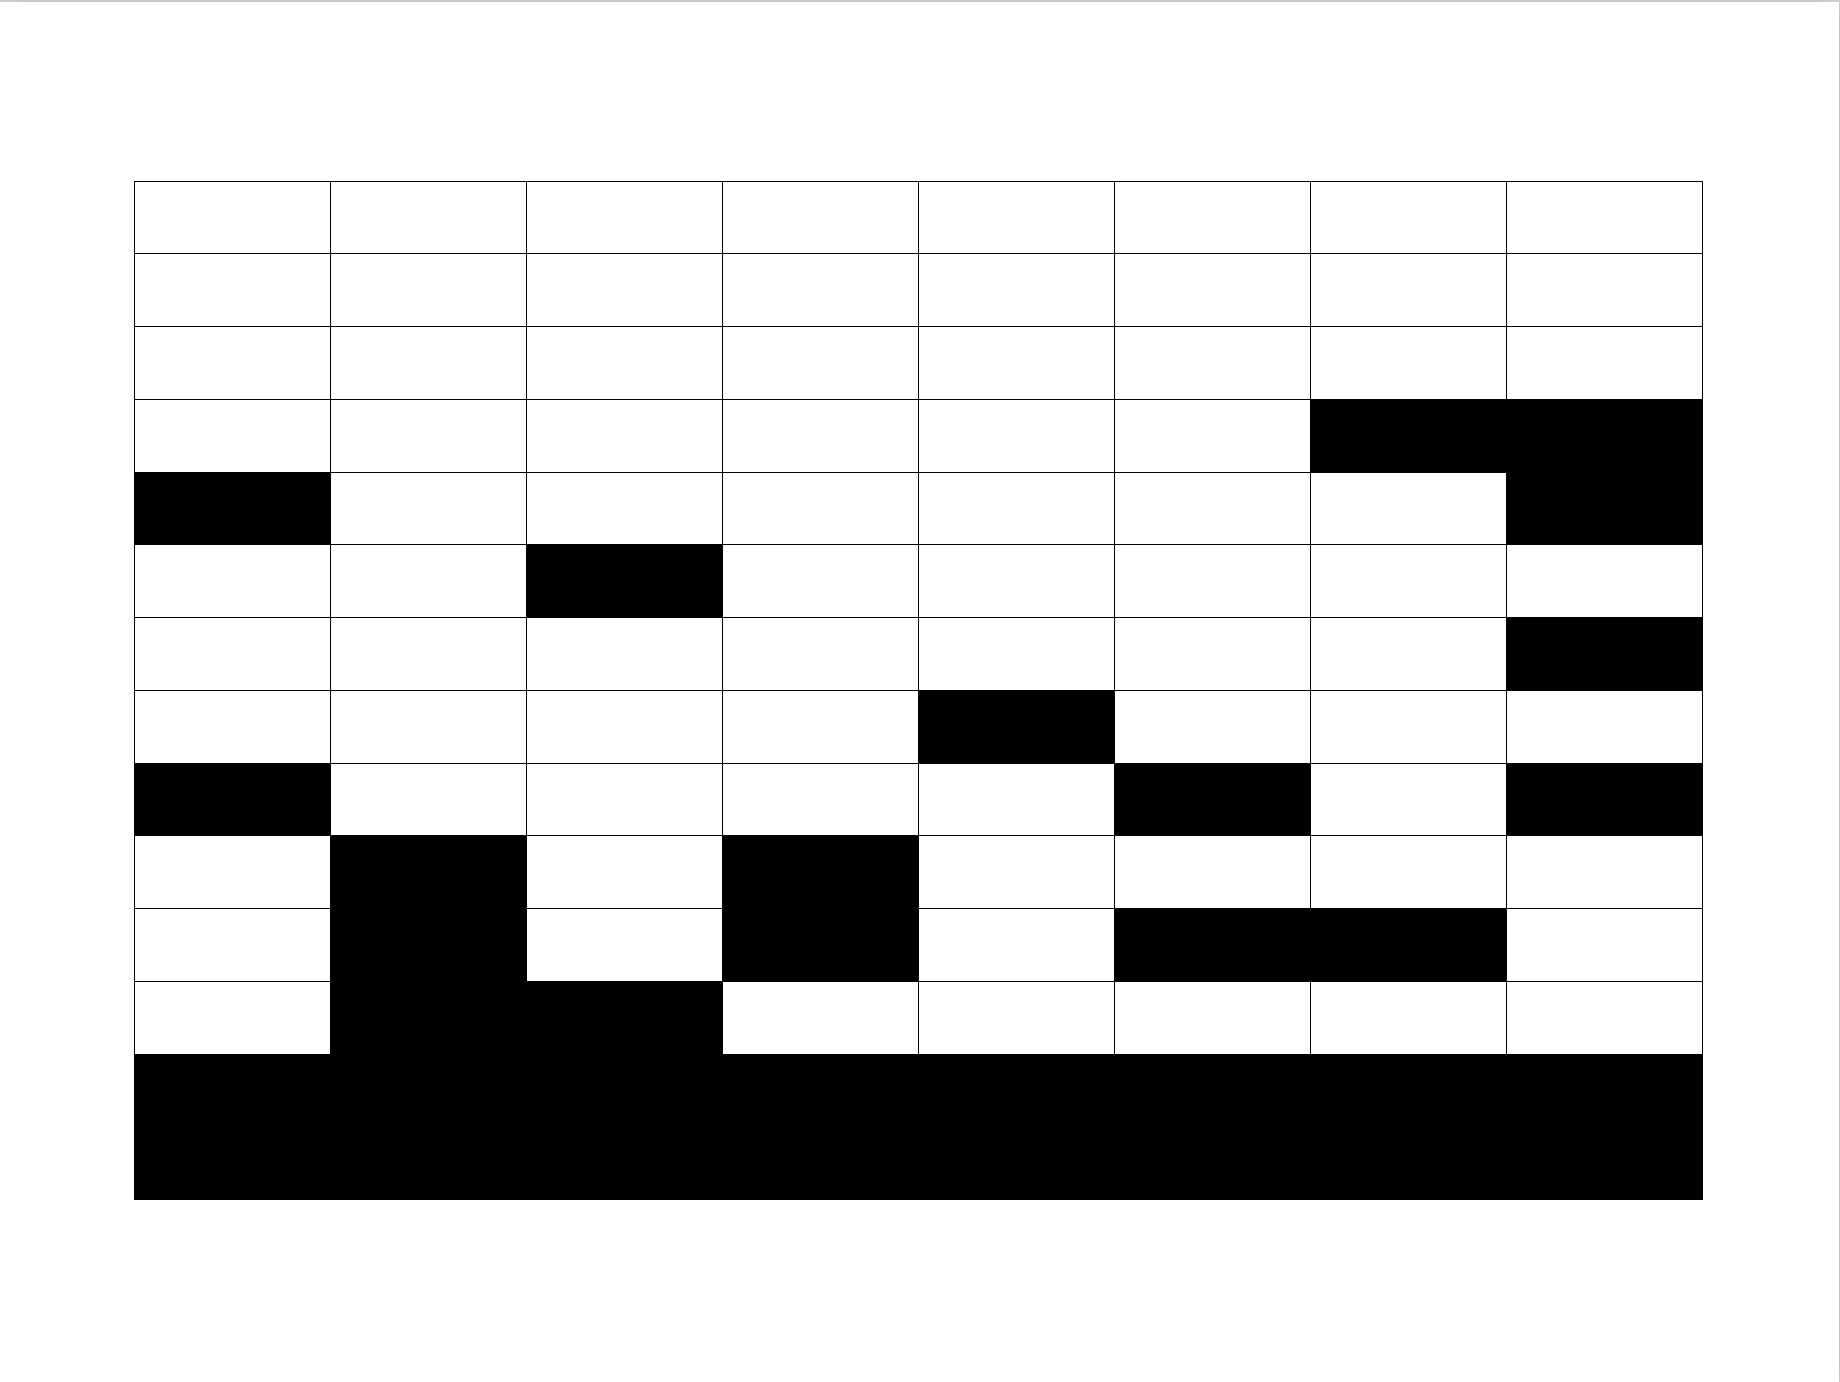
\includegraphics[width=0.5\linewidth]{Pics/j1} \caption{Un conjunto de datos después del proceso de observación.}\label{fig:figbaseincom}
\end{figure}

\hypertarget{imputaciuxf3n-total}{%
\subsection{Imputación total}\label{imputaciuxf3n-total}}

En este enfoque se imputarían todos los valores \(y_k\) que están perdidos, sin importar si la pérdida es debida a la ausencia del registro o del individuo. En este caso, tendríamos un conjunto completo de datos con los valores \(\{y_{\circ \  k}: k\in s\}\), donde

\[
y_{\circ \  k} = 
\begin{cases}
y_k, \ \text{for $k \in r_i$} \\
\hat{y}_k, \ \text{for $k \in s - r_i$}
\end{cases}
\]

y \(\hat{y}_k\) es el valor imputado. Por ejemplo, el estimador del total utilizando este enfoque estaría dado por la siguiente expresión.

\[
\hat{t}_{y,\pi} = \sum_s d_{k}y_{\circ \  k}
= \sum_{r_i}d_{k}y_k + \sum_{s - r_i}d_{k}\hat{y}_k
\]

La figura \ref{fig:figimptotal} muestra un ejemplo de las unidades que serían consideradas para el análisis después de la imputación. Nótese entonces que las tres unidades que respondieron todas las preguntas del cuestionario entran al análisis sin ningún ajuste; mientras que las nueve unidades que no respondieron a todo el cuestionario entran al análisis habiéndose imputado las celdas correspondientes a la ausencia de respuesta; además, las dos unidades que no respondieron ninguna pregunta del cuestionario también entran al análisis puesto que todas sus respuestas fueron imputadas. Luego, en este enfoque todas las unidades en el conjunto \(s\) se consideran para el análisis posterior.

\begin{figure}
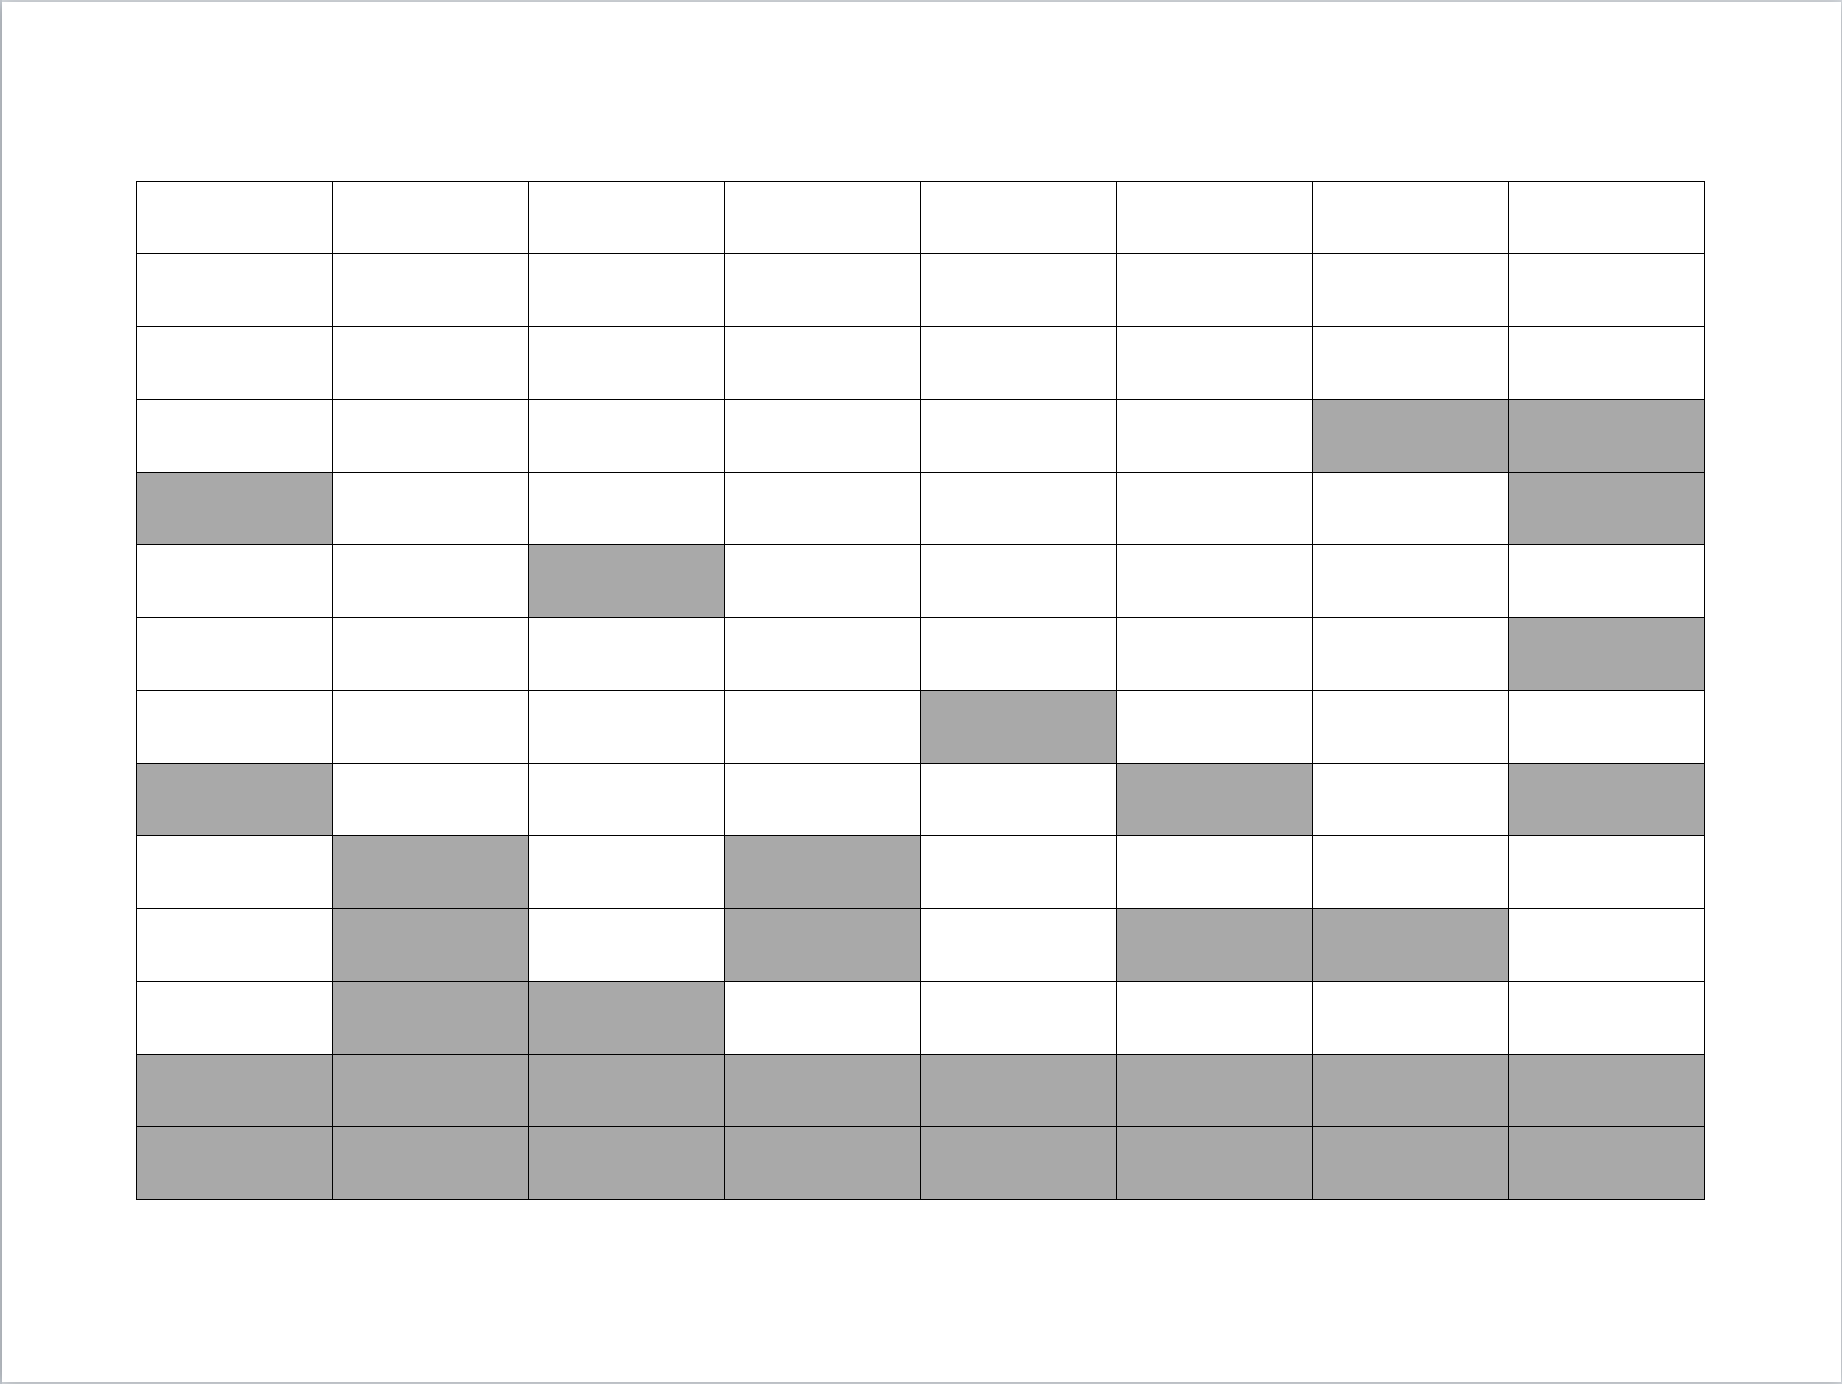
\includegraphics[width=0.5\linewidth]{Pics/j3} \caption{Imputación total: todas las unidades que no respondieron son imputadas (las celdas en gris indican los valores que fueron imputados).}\label{fig:figimptotal}
\end{figure}

\hypertarget{ponderaciuxf3n-total}{%
\subsection{Ponderación total}\label{ponderaciuxf3n-total}}

Al usar el enfoque de ponderación total es posible usar pesos de calibración específicos \(w_k = d_k F_{ik}\) que compensarían la ausencia de respuesta de unidad y de registro. De esta forma, el estimador del total estaría dado por la siguiente expresión:

\[
\hat{t}_{y,cal} =\sum_{r_i}w_ky_k = 
\sum_{r_i}d_k F_{ik} y_k
\]

Si todos los \(r_i\) son diferentes, entonces cada variable de estudio requerirá un conjunto de ponderadores diferentes. Al final este enfoque induce un número no uniforme de casos por variable. Para este esquema, se utilizan pesos \(w_k^{(i)}\) para cada variable \(i \in I\) que compensan la ausencia de respuesta de la unidad. Si todos los \(r_i\) son diferentes, cada variable de estudio requerirá un conjunto de pesos diferente.

Siguiendo con el ejemplo, a partir de la figura \ref{fig:figpondtotal} se nota que la primera variable del cuestionario fue respondida por 10 personas, y cuatro personas no respondieron esta pregunta. Por lo tanto, en este enfoque se crearán pesos \(w_k^{(1)}\) para cada \(k\in r_1\) que ponderen satisfactoriamente la información recolectada en esta variable. Sin embargo, este conjunto de pesos no será único, puesto que, en particular, la segunda variable del cuestionario fue respondida por nueve personas, y tres personas no respondieron esta pregunta. Por lo tanto, en este enfoque se crearán pesos \(w_k^{(2)}\) para cada \(k\in r_2\) que ponderen esta información recolectada en esta variable. Nótese que en general \(w_k^{(1)} \neq w_k^{(2)}\) y, por ende, cada una de las \(I=8\) variables del estudio tendrá su propio conjunto de ponderadores.

\begin{figure}
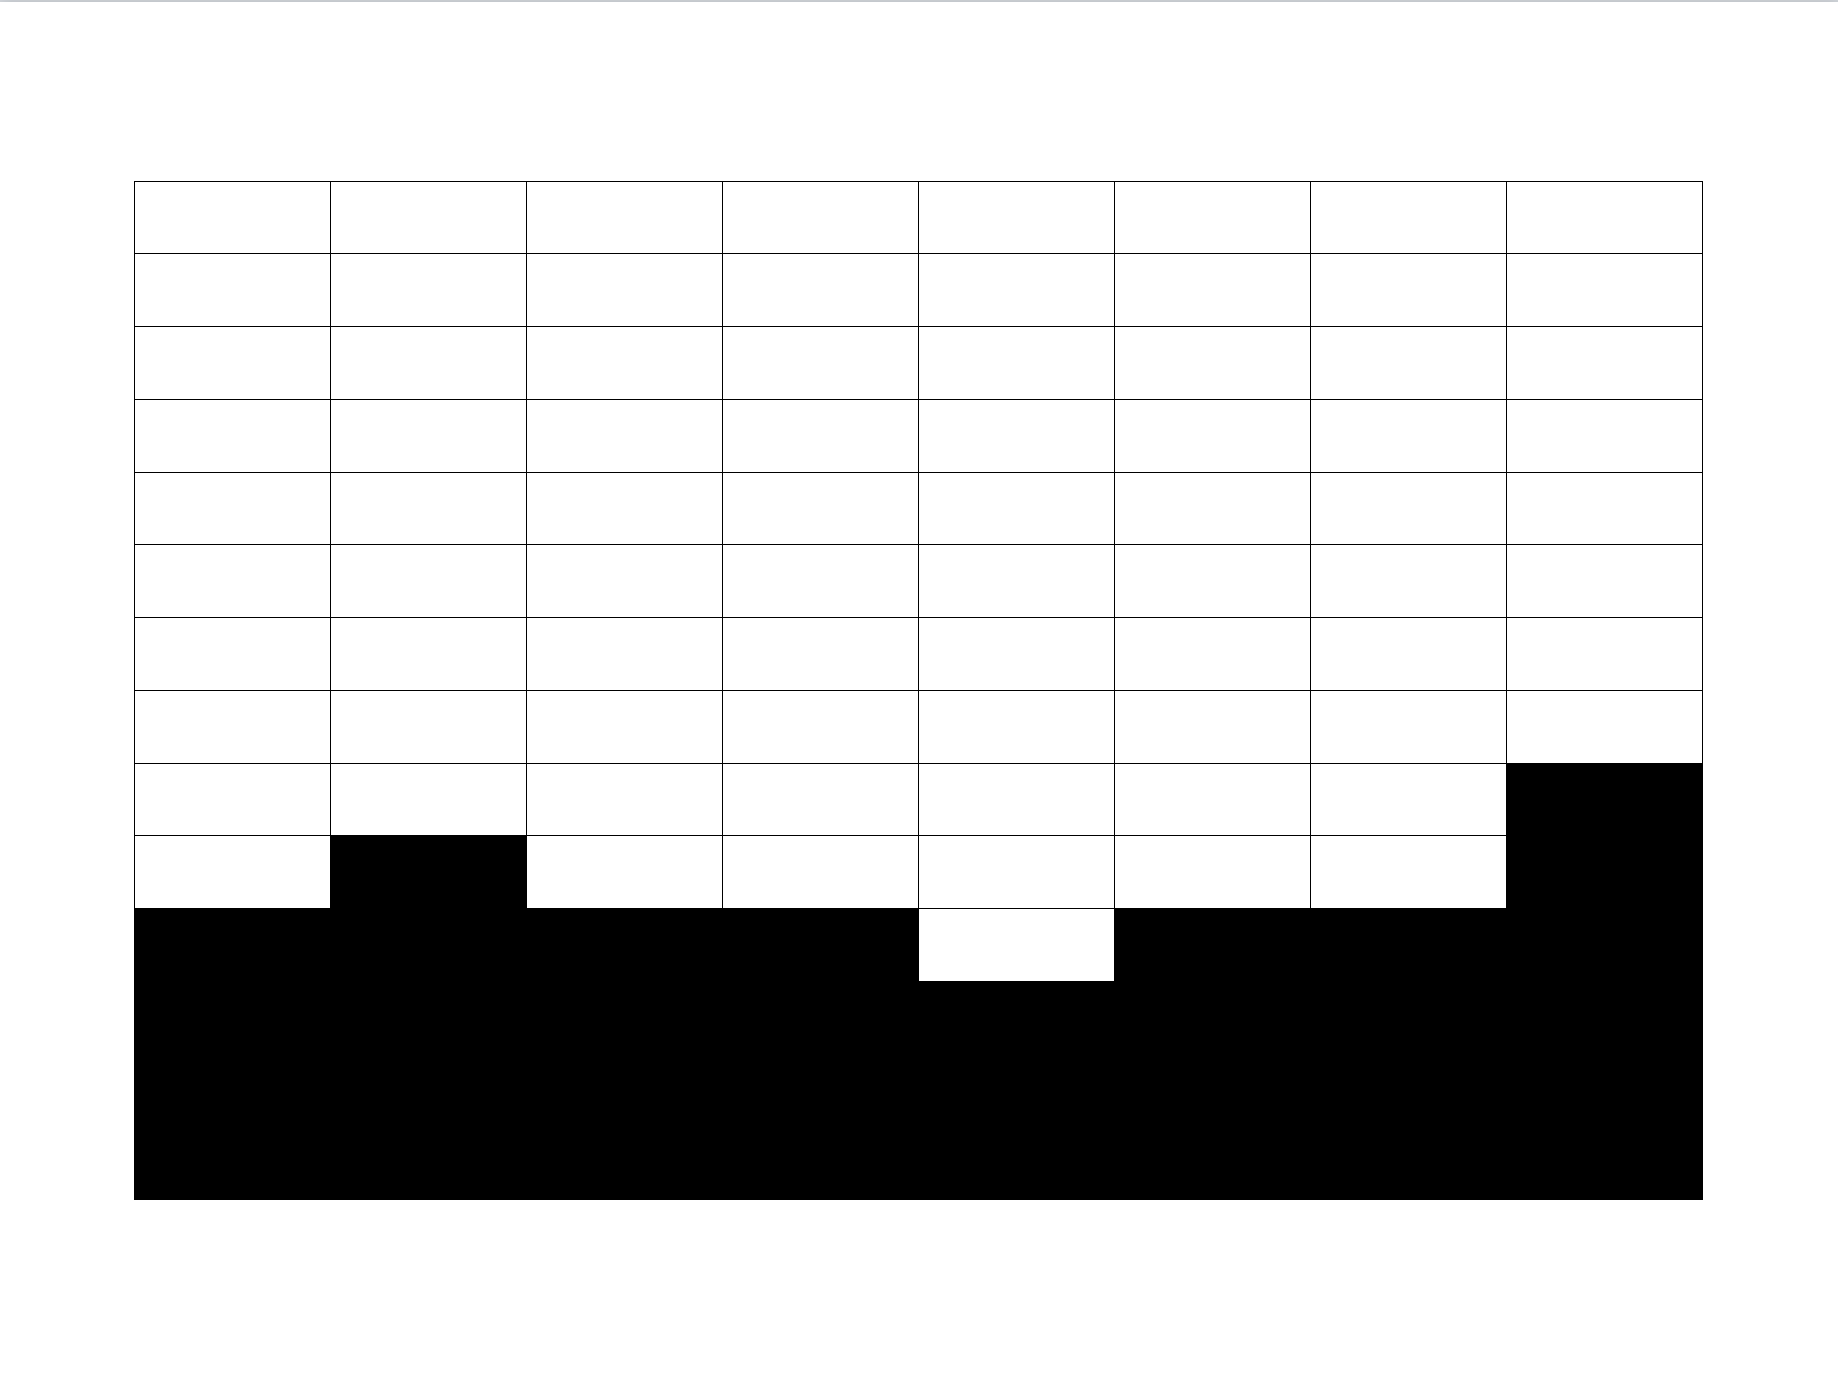
\includegraphics[width=0.5\linewidth]{Pics/j4} \caption{Ponderación total: cada variable tendrá un conjunto de pesos diferente. No se utiliza ningún método de imputación.}\label{fig:figpondtotal}
\end{figure}

\hypertarget{eliminaciuxf3n-total}{%
\subsection{Eliminación total}\label{eliminaciuxf3n-total}}

En este enfoque se eliminarán de la base de datos todas las unidades que contengan al menos un registro perdido. Se recomienda fuertemente abstenerse de tomar este camino, puesto que, aunque induciría un solo conjunto de ponderadores, tendríamos un decrecimiento considerable y deliberado en el tamaño de muestra, asociado con pérdida de información, incremento sustancial de sesgos y decremento de la precisión de los estimadores. Note que en este enfoque sólo las unidades del conjunto de respondientes efectivos en todas las variables se consideran para el análisis posterior de la encuesta. Este subgrupo de individuos está dado por:
\[
\bigcap_{i=1}^I r_i
\]
Por supuesto, en general, esto no es aconsejable puesto que trae problemas de sesgo, dado que las unidades que contestaron todo el cuestionario generalmente difieren de forma estructural de las unidades que no contestaron; además trae problemas de eficiencia estadística, puesto que el tamaño de la muestra efectiva, después de la eliminación de unidades, será insuficiente para garantizar los mínimos requeridos en la inferencia.

La gráfica \ref{fig:figelimtotal} representa este enfoque en donde es evidente que el decrecimiento en el tamaño de muestra podría tener repercusiones nefastas en la inferencia de la encuesta. Teniendo en cuenta el ejemplo anterior, solo tres unidades serían tenidas en cuenta para el análisis de la información, mientras que nueve unidades, que no contestaron al menos una pregunta, más las dos unidades que no contestaron ninguna pregunta, serían eliminadas del análisis estadístico. Es decir, la mayoría de unidades de la muestra inicial serían descartadas.

\begin{figure}

\includegraphics[width=0.5\linewidth]{Pics/j2} \caption{Enfoque de eliminación: únicamente se consideran las unidades que respondedieron a todas las varaibles.}\label{fig:figelimtotal}
\end{figure}

\hypertarget{enfoque-combinado}{%
\subsection{Enfoque combinado}\label{enfoque-combinado}}

Por el contrario, es recomendable escoger un camino parsimonioso que combine estas estrategias de forma diferencial a lo largo de la encuesta. El enfoque combinado usa la imputación para afrontar la ausencia de respuesta por registro para las variables (columnas de la base de datos) específicas que lo necesiten y luego utiliza un ajuste a los factores de ponderación para afrontar la ausencia de respuesta por unidad (filas de la base de datos). Usualmente, los pesos finales se producen utilizando un enfoque de calibración que hace uso de información auxiliar externa.

Cuando se presenta ausencia de respuesta por registro y por unidad, el enfoque combinado imputa primero para luego obtener una matriz rectangular completa. Luego de lo anterior se procede a realizar un ajuste a los ponderadores. El conjunto de datos completo para la variable de interés \(y\) está dado por \(\{y_{\circ \  k}: k\in r\}\)

\[
y_{\circ \  k} = 
\begin{cases}
y_k, \ \text{for $k \in r_i$} \\
\hat{y}_k, \ \text{for $k \in r - r_i$}
\end{cases}
\]

En donde \(\hat{y}_k\) es el valor imputado. Note que en el enfoque de imputación total, también se imputa para \(k \in s-r\). La gráfica \ref{fig:figenfcomb} representa este enfoque parsimonioso en donde los valores imputados (en gris) entran a ser parte de la inferencia y las unidades que nunca respondieron (en negro) y que tienen todos sus registros faltantes son retiradas de la base de datos final.

Se observa que los dos últimos individuos de la muestra fueron totalmente descartados puesto que no contestaron ninguna pregunta del cuestionario; además, para la primera variable, los valores del quinto y noveno individuo fueron imputados. De la misma manera, para la segunda variable, los valores de los individuos diez, once y doce fueron imputados; y así sucesivamente, hasta llegar a la última variable en donde los valores de los individuos cuatro, cinco, siete y nueve fueron imputados.

\begin{figure}
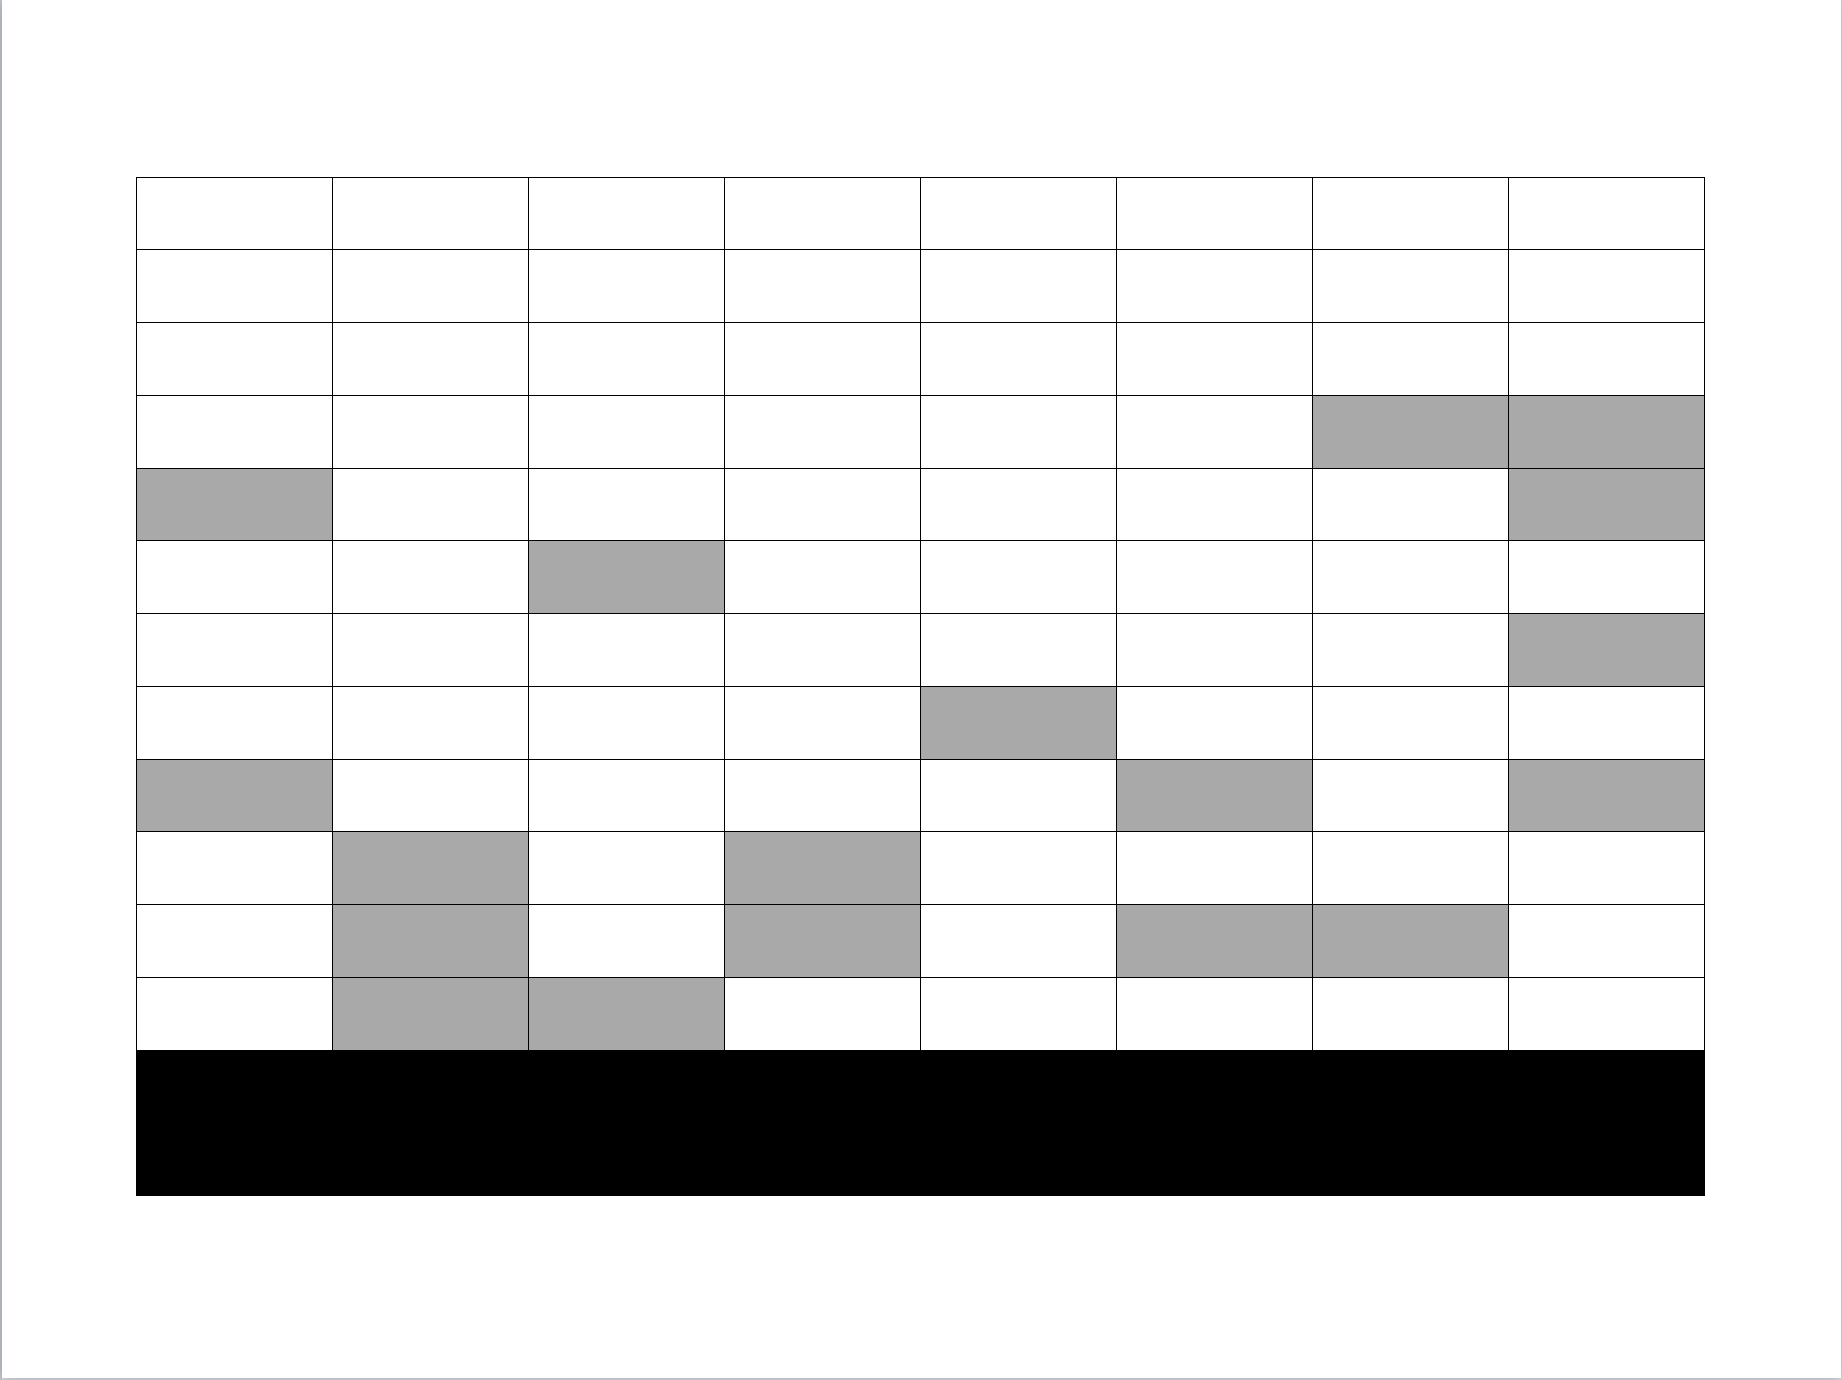
\includegraphics[width=0.5\linewidth]{Pics/j5} \caption{Enfoque combinado: las unidades que no respondieron a ningún ítem son eliminadas del análisis y los respondientes parciales son imputados.}\label{fig:figenfcomb}
\end{figure}

Los capítulos anteriores profundizaron en el tema de la creación de factores de expansión para los individuos presentes en la base de datos final. De tal forma que en los capítulos posteriores se abordará algunas metodologías de imputación que pueden ser recomendables a la hora de completar una base de datos estructurada y rectangular cuyas entradas estén completas. Antes de introducir estos temas se presentarán algunas medidas descriptivas que pueden ser usadas para generar alertas sobre la pérdida de representatividad debido a la ausencia de respuesta.

\hypertarget{ausencia-de-respuesta-de-unidad}{%
\chapter{Ausencia de respuesta de unidad}\label{ausencia-de-respuesta-de-unidad}}

En una encuesta la información auxiliar puede utilizarse en dos etapas: en la planeación del diseño de muestreo y en la escogencia del estimador. En el primer caso, es posible utilizar la información auxiliar para construir estratos, definir conglomerados, asignar los tamaños de muestra dentro de los estratos, o incluso construir probabilidades de selección desiguales. De la misma forma, en el segundo caso, la información auxiliar puede utilizarse en la estimación de los parámetros de interés al definir nuevos ajustes de ponderación, al imponer restricciones de consistencia con la información auxiliar disponible a nivel de censos, registros o encuestas para que la distribución de la muestra expandida coincida plenamente con algunas características poblacionales. En este capítulo se aborda el uso de la información auxiliar en el estimador para corregir los sesgos generados por la ausencia de respuesta.

Como se ha expuesto anteriormente, la ausencia de respuesta a nivel de unidad puede tener consecuencias muy graves en la inferencia resultante de las encuestas de hogares, puesto que si el conjunto de respondientes tiene características distintas al conjunto de no respondientes, entonces se introducirá sesgo en la estimación de los parámetros de interés.

\hypertarget{sesgo-sobre-los-estimadores}{%
\section{Sesgo sobre los estimadores}\label{sesgo-sobre-los-estimadores}}

Asumiendo que existe ausencia de respuesta en la muestra, considere la siguiente forma de estimar (ingenuamente) el promedio poblacional \(\bar{y}_U\) mediante el estimador de Hájek

\[
\tilde{y}_s = \frac{\sum_{s_r}d_ky_k}{\sum_{s_r}d_k} = \frac{\hat{t}_y}{\hat{N}}
\]

Siendo \(\bar{\phi}\) el promedio de las probabilidades de respuesta, el sesgo generado por la ausencia de respuesta puede cuantificarse de la siguiente manera:

\[
B\left(\tilde{y}_s\right)  = 
\frac{1}{N\bar{\phi}}\sum_U(y_k-\bar{y}_U)(\phi_k-\bar{\phi})
= \frac{Cov\left(\bar{y},\phi\right)}{\bar{\phi}}
= \frac{Cor\left(Y,\phi\right)S\left(Y\right)S\left(\phi\right)}{\bar{\phi}}
\]

En donde \(Cov\left(Y,\phi\right)\) es la covarianza poblacional entre
los valores de la característica de interés y las probabilidades de respuesta,
\(cor\left(Y,\phi\right)\) es el coeficiente de correlación poblacional
y \(S\left(Y\right)\) es la desviación estandar poblacional de la variable objetivo. Dado que el valor del coeficiente de correlación está restringido
al intervalo \([-1, 1]\), el valor máximo del sesgo absoluto será igual a

\[
|B\left(\tilde{y}_s\right)| \leq 
\frac{S\left(\phi\right)S\left(y\right)}{\bar{\phi}}
= \frac{\left(1-R\left(\phi\right)\right)S\left(y\right)}{2\bar{\phi}}
\]

A pesar de que este límite superior no se puede calcular en situaciones prácticas, sí es posible estimarlo utilizando los datos de la muestra y las probabilidades
de respuesta estimadas. Nótese que si el mecanismo de ausencia de respuesta fuese MCAR, entonces el valor de \(R\left(\phi\right)\) sería uno, y por consiguiente no habría sesgo. De la misma forma, en el caso extremo en el que la característica de interés fuese homogénea en toda la población, tampoco habría sesgo en el estimador, y bastaría con utilizar los datos de la muestra de respondientes efectivos, sin ningún tipo de corrección.

Además de las anteriores consideraciones, es posible evaluar las propuestas de escogencia de variables para calibración de \citet{KaltonFloresCervantes_2003} y de \citet{Sarndal_2011}. En particular, este último autor considera un indicador del sesgo por ausencia de respuesta sobre los estimadores de calibración, cuya lógica se basa en que, en el mejor de los casos, en el que no hubiese errores de cobertura ni ausencia de respuesta, el estimador de expansión \(\hat{t}_{y}\) sería insesgado y la distancia que habría entre este y el estimador de calibración \(\hat{t}_{y,cal}\) se podría cuantificar como \(\Delta_A = \frac{(\hat{t}_{y,cal} - \hat{t}_{y})}{N}\). Este indicador se sugiere como una posible herramienta para comparar potenciales variables de calibración, de tal forma que cuando el valor de \(|\Delta_A|\) sea grande habría un indicio para preferir un vector de calibración sobre otro. Además, al estandarizarla, esta medida puede ser descompuesta en los siguiente tres factores:

\[\frac{\Delta_A}{S_y} = cv_g \ \times R_{y,\mathbf{x}} \ \times R_{D,C}\]

De esta forma, el primer factor representa el coeficiente de variación de los pesos \(g_k\); el segundo factor al cuadrado es el coeficiente de determinación de una regresión múltiple entre la variable de estudio y las variables del vector de calibración; el último factor al cuadrado es el coeficiente de determinación (proporción de varianza explicada) en una regresión ponderada que pasa por el origen entre las desviaciones de las covariables \(D_j = \hat{t}_{x, j} - t_{x,j}\) y las covarianzas de la variable de estudio y las covariables \(C_j = cov(y, x_j)\).

\hypertarget{soluciones}{%
\section{Soluciones}\label{soluciones}}

Como se expuso en la sección anterior, si no hay correlación entre la variable de interés y la estructura de la ausencia de respuesta entonces no hay sesgo en los estimadores. Esto quiere decir que, si la probabilidad de respuesta es homogénea (representatividad fuerte) o pudiera modelarse (representatividad débil) para todos los individuos, entonces el sesgo se podría eliminar. En esta sección se explorarán dos caminos que, al incorporar información auxiliar, eliminan el sesgo causado por el fenómeno de la ausencia de respuesta.

Ambas opciones, ajuste de factores de expansión mediante modelos de \emph{propensity score} y estimadores de calibración, descansan en el paradigma de la inferencia basada en el diseño de muestreo y por ende se contemplan como dos posibilidades atractivas que mantienen la buenas propiedades de la estimación directa en encuestas de hogares.

\hypertarget{propensity-score}{%
\subsection{Propensity Score}\label{propensity-score}}

Como se mencionó anteriormente, uno de los ajustes que se debe realizar en la generación de los ponderadores finales es la corrección por ausencia de respuesta. En donde

\[d_{4k} =  \frac{d_{3k}}{\hat{\phi_k}}\]

Como ya se había mencionado en los capítulos anteriores, si el patrón de ausencia de respuesta es NMAR, entonces \(\phi_k = f(\mathbf{y}_k, \beta)\) y en este caso, como no es posible tener acceso a los determinantes de la respuesta (porque precisamente son las mismas variables de interés en la encuesta), entonces no es posible estimar el patrón de ausencia de respuesta. Por ende, en este escenario habrá sesgo siempre. Por el contrario, si el patrón de ausencia de respuesta es MCAR o MAR, entonces \(\phi_k = f(\mathbf{x}_k, \boldsymbol{\beta})\); en este caso, si fuese posible tener acceso a las covariables \(\mathbf{x}\) que determinan el mecanismo de respuesta, entonces es posible estimar las probabilidades de respuesta mediante \(\hat{\phi}_k = f(\mathbf{x}_k, \hat{\boldsymbol{\beta}})\). Efectivamente, en el caso del estimador de Horvitz-Thompson, el sesgo del estimador se anula puesto que

\begin{align*}
E(\hat{t}_y) &= E\left(\sum_{k\in s_r}d_{3k}y_k\right) \\
&= E\left(\sum_{k\in s_r}\frac{y_k}{\pi_k \hat{\phi_k}}\right)\\
&= E\left(E\left(\sum_{k\in U}\frac{y_k}{\pi_k \hat{\phi_k}}I_kD_k|I_k\right)\right)\\
&= \sum_{k\in U}\frac{y_k}{\pi_k \hat{\phi_k}}E\left(I_k\right)E\left(D_k|I_k\right)\\
&= \sum_{k\in U}\frac{y_k}{\pi_k \hat{\phi_k}}\pi_k\phi_k = t_y
\end{align*}

Asumiendo que el modelo está bien establecido, entonces se tendrá una concordancia directa entre \(\hat{\phi_k}\) y \(\phi_k\); por lo tanto se anularían en la última igualdad de la ecuación anterior. Además, el insesgamiento viene supeditado puesto que,

\[
E(I_kD_k) 
= E\left(E(I_kD_k|I_k) \right)
= E(I_k)E(D_k|I_k) = \pi_k \phi_k
\]

En resumen, si se tiene acceso a información auxiliar (contenida en el marco de muestreo o en otras preguntas de la encuesta), y si se considera que el mecanismo que genera la ausencia de respuesta en la encuesta de hogares es MAR o MCAR, es posible ajustar un modelo de \emph{propensity score} para la ausencia de respuesta (en donde la variable dependiente es una variable indicadora de la respuesta del individuo por lo general supeditado a una distribución Bernoulli o Binomial). En resumen, es posible definir el siguiente estimador insesgado

\[
\hat{t}_y=\sum_{k\in s_{ER}}d_{4k}y_k
\]

En donde

\[
d_{4k} = \frac{d_{3k}}{\hat{\phi_k}}  \ \ \ \ \ \ \ \ \forall \ k  \in s_{ER}
\]

Siempre es muy importante realizar una validación exhaustiva de los modelos utilizados para estimar la probabilidad de respuesta. En general, es necesario que el modelo satisfaga las siguientes dos condiciones:

\begin{enumerate}
\def\labelenumi{\arabic{enumi}.}
\tightlist
\item
  \emph{Soporte común}: al igual que en un experimento aleatorizado, es necesario garantizar que ninguna combinación de las covariables induzca un estado (respuesta o ausencia de respuesta) de forma determinística. Es decir sobre todas las combinaciones en las covariables deben existir respondientes y no respondientes. Esta condición se puede escribir como:
  \[
  0 < Pr(D_{1,k} = 1 |\mathbf{x}_{1}) < 1 
  \]
\item
  \emph{Balanceo}: como la respuesta de las unidades de muestreo no provienen de un estudio aleatorizado, es necesario garantizar que la distribución de las \(\hat\phi_k\) sea similar entre respondientes y no respondientes. De esta forma, es posible expandir el subconjunto de respondientes efectivos a la muestra original (que incluye a las unidades no respondientes), la cual a su vez expande a toda la población de interés. Esta condición se puede escribir como:
\end{enumerate}

\begin{align*}
\hat\phi_{1, k} &= Pr[D_{1, k} | I_{1, k} = 1,\mathbf{x}] \\
&= Pr[D_{1, k} | k \in s_r, I_{1, k} = 1, \mathbf{x}] \\
&= Pr[D_{1, k} | k \notin s_r, I_{1, k} = 1, \mathbf{x}]
\end{align*}

Por último, se debe corroborar que la suma de los pesos ajustados por la ausencia de respuesta esté cercana al tamaño de la población que se quiere representar. La figura \ref{fig:figel3a} permite ilustrar el soporte común entre respondientes y no respondientes para un modelo de \emph{propensity score}; nótese que ambas distribuciones son similares, por lo que es posible concluir que efectivamente las covariables usadas están representando bien la estructura estocástica en respondientes y no respondientes.

\begin{figure}

{\centering 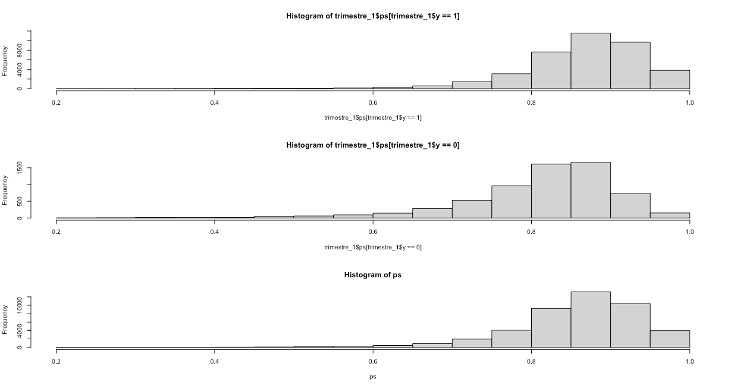
\includegraphics[width=0.5\linewidth]{Pics/el3a} 

}

\caption{Distribución de las probabilidades estimadas de respuesta: respondientes (arriba), no respondientes (medio), ambos (abajo).}\label{fig:figel3a}
\end{figure}

Además, la figura \ref{fig:figel3b} muestra la propiedad de balanceo en el modelo; véase cómo ambas distribuciones se alejan de los extremos (ceros y uno) y presentan una caracterización similar.

\begin{figure}

{\centering 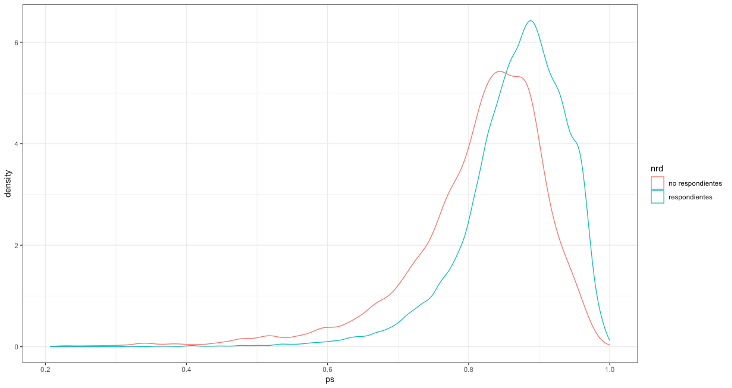
\includegraphics[width=0.5\linewidth]{Pics/el3b} 

}

\caption{Balanceo entre respondientes y no respondientes}\label{fig:figel3b}
\end{figure}

\hypertarget{calibraciuxf3n}{%
\subsection{Calibración}\label{calibraciuxf3n}}

Como lo afirma \citet{Sar08}, la calibración provee una forma sistemática para involucrar la información auxiliar. En la mayoría de aplicaciones prácticas, la calibración provee un enfoque simple para incorporar esta información dentro de la etapa de estimación. La información auxiliar fue usada para mejorar la precisión de los estimativos mucho antes que el término calibración fuera popular. La calibración puede ser usada efectivamente en encuestas donde la información auxiliar está disponible en diferentes niveles. Por ejemplo, al realizar un muestreo en dos etapas la información auxiliar puede existir para las unidades de la primera etapa (los conglomerados) y puede existir otra información para las unidades de la segunda etapa (elementos o conglomerados).

Como se ha detallado con amplitud en este y los capítulos anteriores, la ausencia de respuesta de unidad tiene consecuencias dañinas en la inferencia con encuestas de hogares. En este caso es altamente recomendable que se implemente ajuste a los factores de ponderación de las unidades (hogares o personas). A pesar de que los modelos de \emph{propensity score} tienen una larga trayectoria en el manejo de la ausencia de respuesta, la calibración utilizada para corregir estos sesgos ofrece una relativamente nueva perspectiva. Nótese que el estimador tradicional toma la siguiente forma:

\[
\hat t_y^* = \sum_{s_r} w_k\ y_k = \sum_{s_r} \frac{d_k}{\phi_k} y_k 
\]

Esta anterior expresión indica que implícitamente se genera un procedimiento en dos etapas en donde, en primer lugar, se calculan lo pesos básicos inducidos por el diseño de muestreo, luego se ajusta un modelo de \emph{propensity score} para estimar las probabilidades de respuesta \(\phi_k\). A esta estrategia generalmente se le agrega una tercera etapa en donde se crean nuevos pesos calibrados con respecto a proyecciones demográficas post-censales, como por ejemplo los cruces entre edad, sexo y región. Al ajustar los pesos para que sumen exactamente la cifra de las proyecciones censales, se reduce el sesgo de subcobertura.

\citet{Sar08} afirma que la práctica general es asumir que el estimador \(\hat t_y^*\) es insesgado, cuando en realidad no lo es, puesto que no es posible conocer todos los determinantes del mecanismo de respuesta para ajustar el modelo que estima las probabilidades de respuesta. Además, de la sección anterior se deduce que este supuesto implica que se considere que \(\pi_k \hat\phi_k\) es la verdadera probabilidad de inclusión de la unidad, cuando en realidad no es así. Por lo tanto, realizar un ajuste a los factores de expansión únicamente basados en los modelos de \emph{propensity score} traerá inevitablemente una cierta cantidad de sesgo en la estimación de los parámetros en las encuestas de hogares.

Bajo este escenario, el enfoque de calibración doble surge como un proceso metodológico adicional que pretende corregir estos sesgos. Para poder utilizarlo, es necesario tener información auxiliar en dos niveles: la población y la muestra. Este tipo de metodologías pueden ser usadas en las encuestas tipo panel, o panel rotativo. En este proceso es necesario contar con dos tipos de información auxiliar:

\begin{enumerate}
\def\labelenumi{\arabic{enumi}.}
\tightlist
\item
  Por un lado tendremos la información poblacional usual que se utiliza para calibrar los factores de expansión en un levantamiento regular. Las variables que intervienen en esta calibración las notaremos como \(\boldsymbol{x}_{1k}\) y por lo general denotan la pertenencia de los individuos a regiones, o grupos de edad, sexo o área (urbano, rural).
\item
  Por otro lado deberemos tener acceso a información auxiliar en la muestra original (que incluya a las unidades respondientes y no respondientes) y que notaremos como \(\boldsymbol{x}_{2k}\). Por ejemplo, utilizando la información del panel al momento de la primera medición, sería posible contar con información concerniente a la condición de ocupación, ingresos, o cualquier otra variable medida en la primera oleada del panel.
\end{enumerate}

Por lo tanto, es posible calibrar los pesos en la muestra de respondientes (\(s_r\)) a nivel de la información auxiliar disponible en la muestra original (\(s\)), y luego a nivel nacional (\(U\)) o por los estratos de interés. Si el mecanismo que genera la ausencia de respuesta es MAR o MCAR, es posible que los ponderadores de calibración eliminen el sesgo en las estimaciones finales si es que las variables que generan este mecanismo se han calibrado en alguno de las dos niveles mencionados. \citet{Sarndal_Lundstrom_2006} proponen que, para lograr este objetivo, se encuentre un primer conjunto de pesos calibrados sujetos a la siguiente restricción:

\[
\sum_{s}w_{1k}\boldsymbol{x}_{1k} = \sum_{U}\boldsymbol{x}_{1k}
\]

Luego, en una segunda etapa, se deben usar estos pesos intermedios \(w_{1k}\) para calcular los pesos finales de calibración \(w_{k}\) de la muestra de respondientes efectivos que están sujetos a la siguiente restricción:

\[
\sum_{s_r}w_{k}\boldsymbol{x}_{2k} = \sum_{s}w_{1k}\boldsymbol{x}_{k} = 
\begin{pmatrix}
\sum_{U}\boldsymbol{x}_{1k}\\
\sum_{s_r}w_{1k}\boldsymbol{x}_{2k}
\end{pmatrix}
\]

En este sentido, nótese que la forma funcional de los pesos de calibración doble resultantes de este proceso de optimización se pueden escribir de la siguiente manera:

\[
w_k = d_k \times g_k  \cong d_k \times \hat \phi_k
\]

Por ende, bajo el raciocinio de la calibración, los pesos \(g_k\) se pueden ver como una estimación de las probabilidades de respuesta \(\phi_k\). Por otra parte, de las expresiones, sobre el sesgo de los estimadores que no contienen ningún tipo de corrección, se puede notar que el sesgo se propaga a través de las variables de la encuesta y se propaga con más fuerza en las variables correlacionadas con los determinantes de la ausencia de respuesta.

Para mostrar cómo el ajuste a los factores de expansión, con las dos metodologías anteriormente mencionadas, inducen menor sesgo que los estimadores comunes, se planeó el siguiente experimento:

\begin{enumerate}
\def\labelenumi{\arabic{enumi}.}
\tightlist
\item
  Se generó una población compuesta por individuos con diferente propensión de respuesta MCAR.
\item
  Se utilizaron metodologías de calibración y se comparó, de forma empírica, el efecto de la ausencia de respuesta sobre las estimaciones finales.
\end{enumerate}

En primera instancia, cabe mencionar que la población se definió a partir del ingreso del hogar, y se creó usando variables auxiliares disponibles (sexo). De esta forma, se le dio una probabilidad de respuesta diferencial entre los grupos correspondientes al cruce de las categorías de estas dos variables. Como resultado de las simulaciones, se generaron estimaciones para el estimador de Horvitz-Thompson sin ajuste de ningún tipo y para un estimador de calibración que tuvo en cuenta los conteos poblacionales censales para cada las dos categorías de la variables sexo. La figura \ref{fig:fightcal} muestra el comportamiento de ambas estimaciones. La línea roja refleja el parámetro desconocido, los puntos negros indican las estimaciones del estimador de calibración en cada iteración de la simulación, mientras que los puntos grises muestran las estimaciones del estimador de Horvitz-Thompson en cada iteración de la simulación

\begin{figure}

{\centering 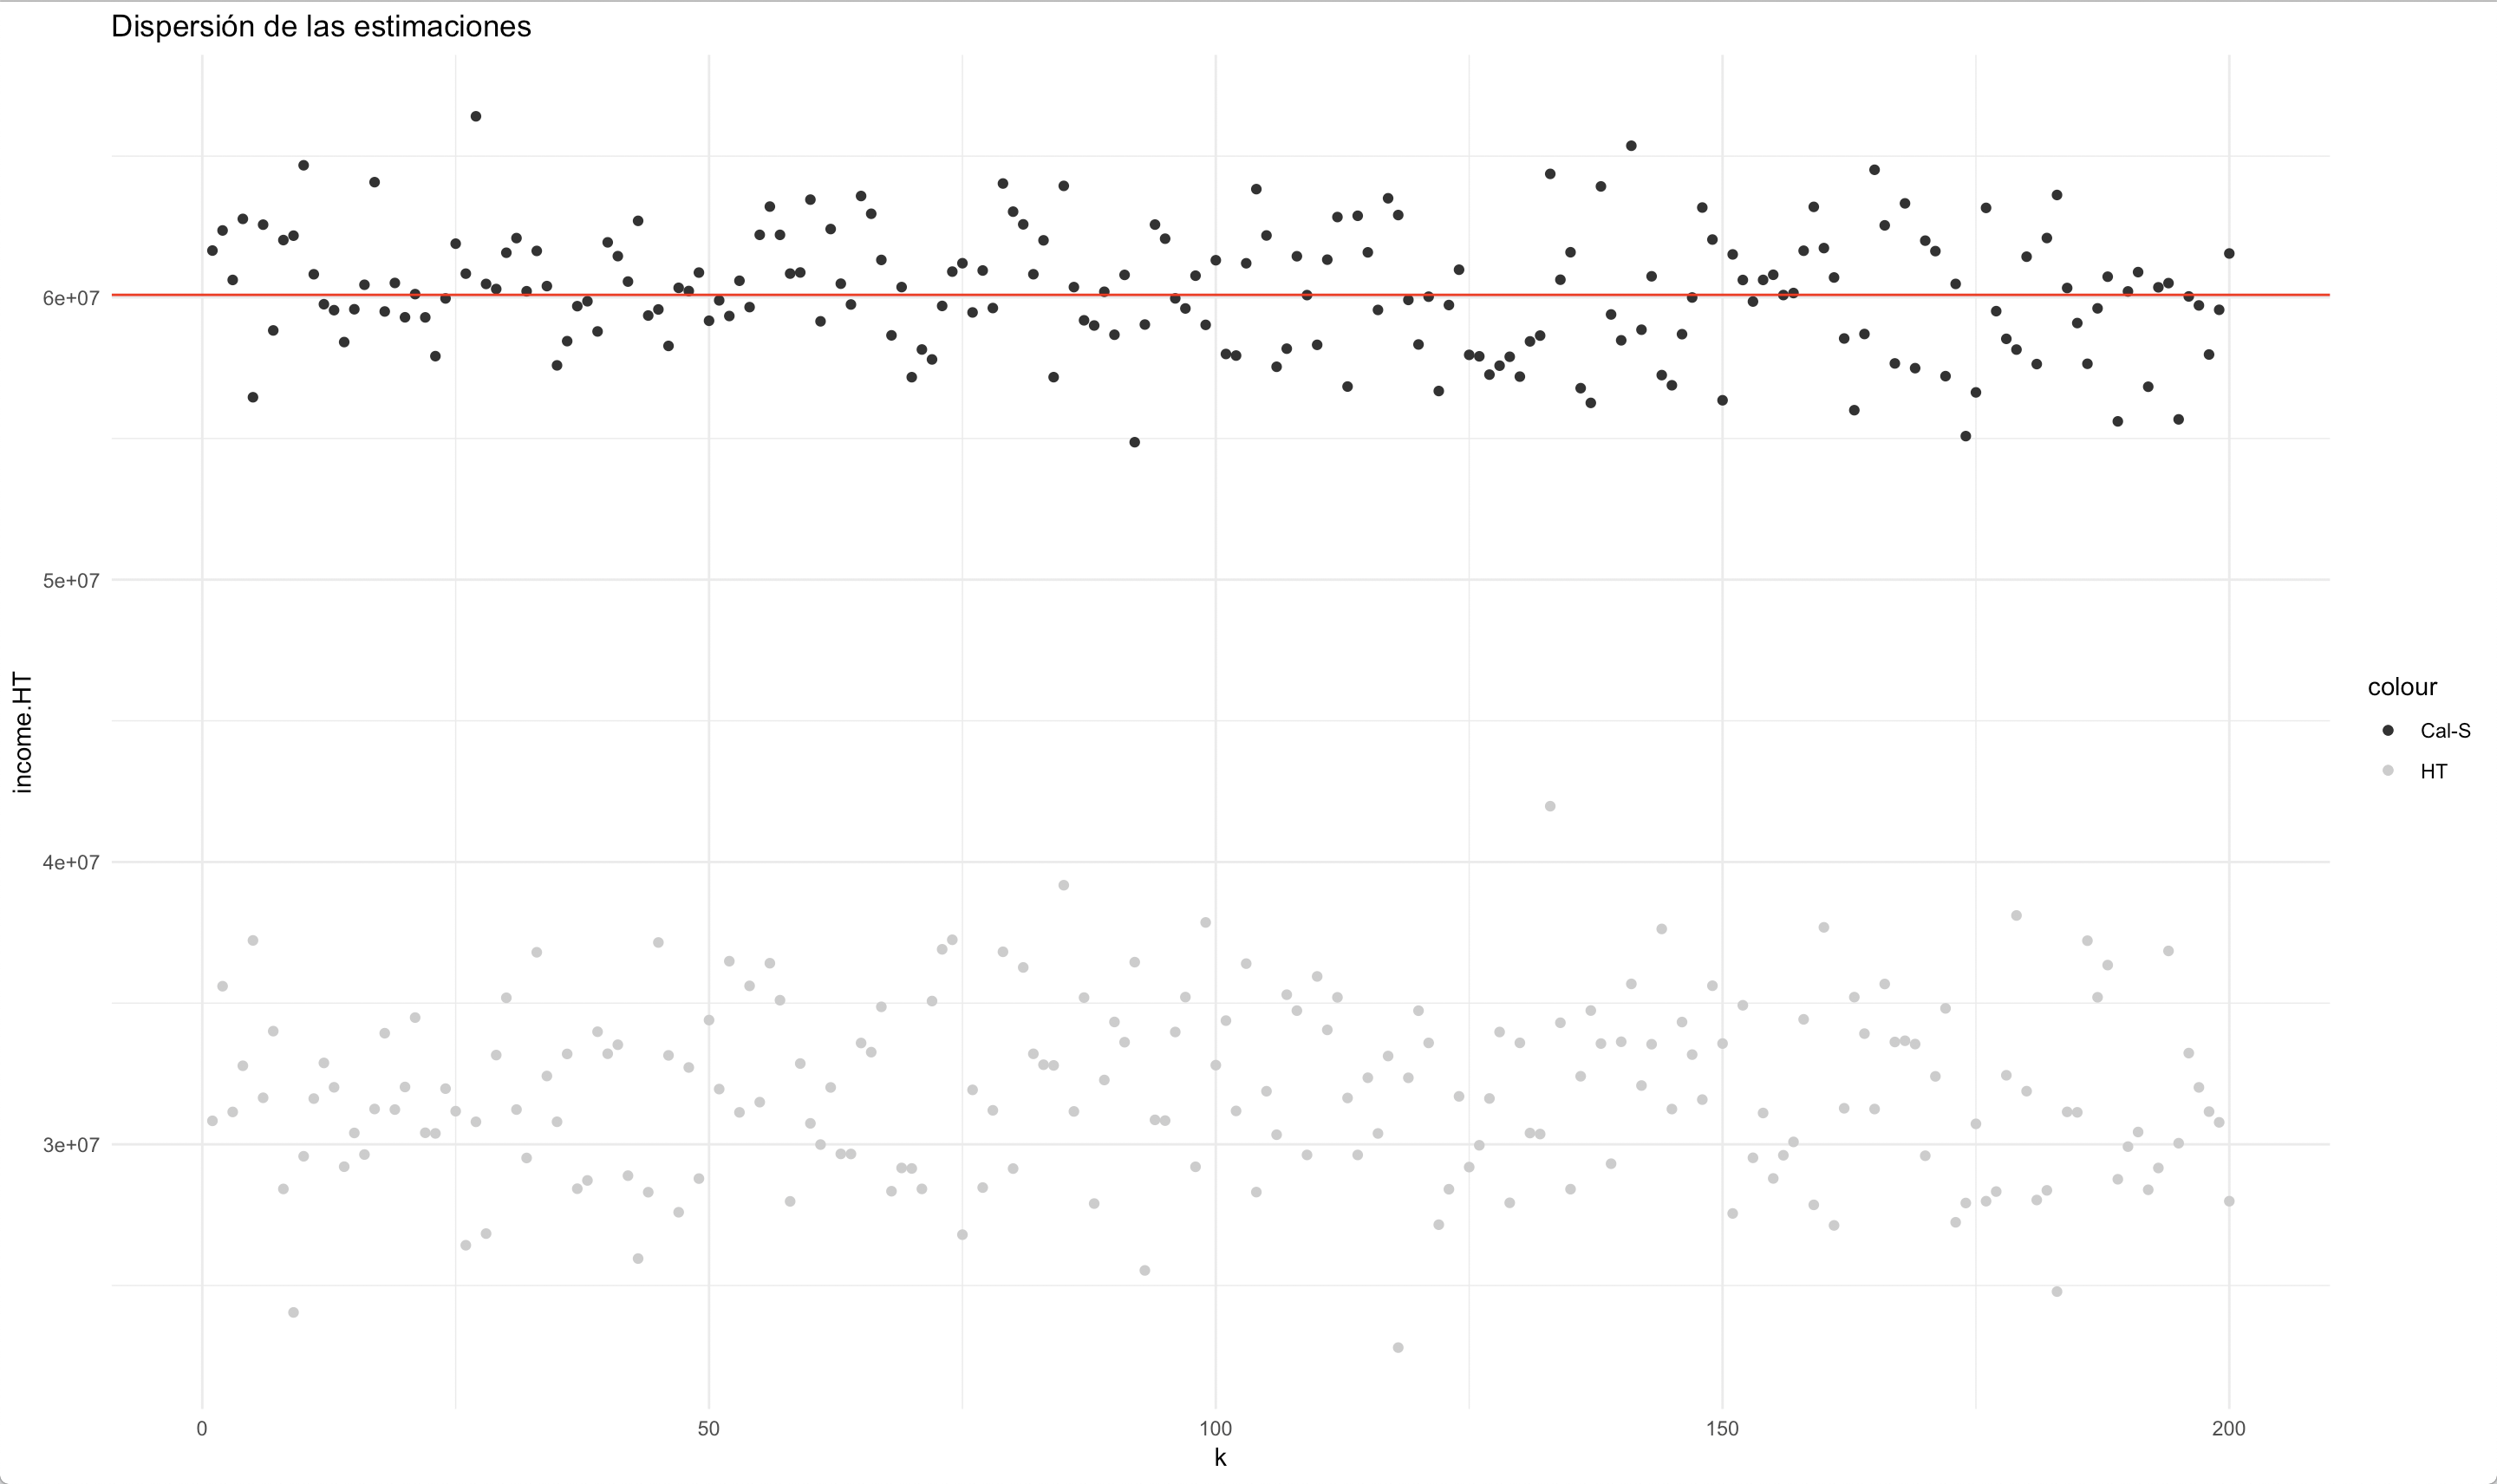
\includegraphics[width=0.5\linewidth]{Pics/c9} 

}

\caption{Estimaciones de Horvtiz-Thompson y de calibración.}\label{fig:fightcal}
\end{figure}

En conjunto con la gráfica anterior, la figura \ref{fig:fightcaldist} muestra la distribución sesgada del estimador de Horvitz-Thompson (gris) en comparación con el insesgamiento del estimador de calibración (negro). Bajo este esquema de respuesta, incluir en la calibración las variables pertinentes corrige el sesgo generado por la ausencia de respuesta. En este estudió se encontró que el estimador ingenuo (HT) produjo sesgo para la estimación de los tamaños de hombres y mujeres, para el tamaño de la población, para los ingresos de hombres y mujeres y para los ingresos de la población.

\begin{figure}

{\centering 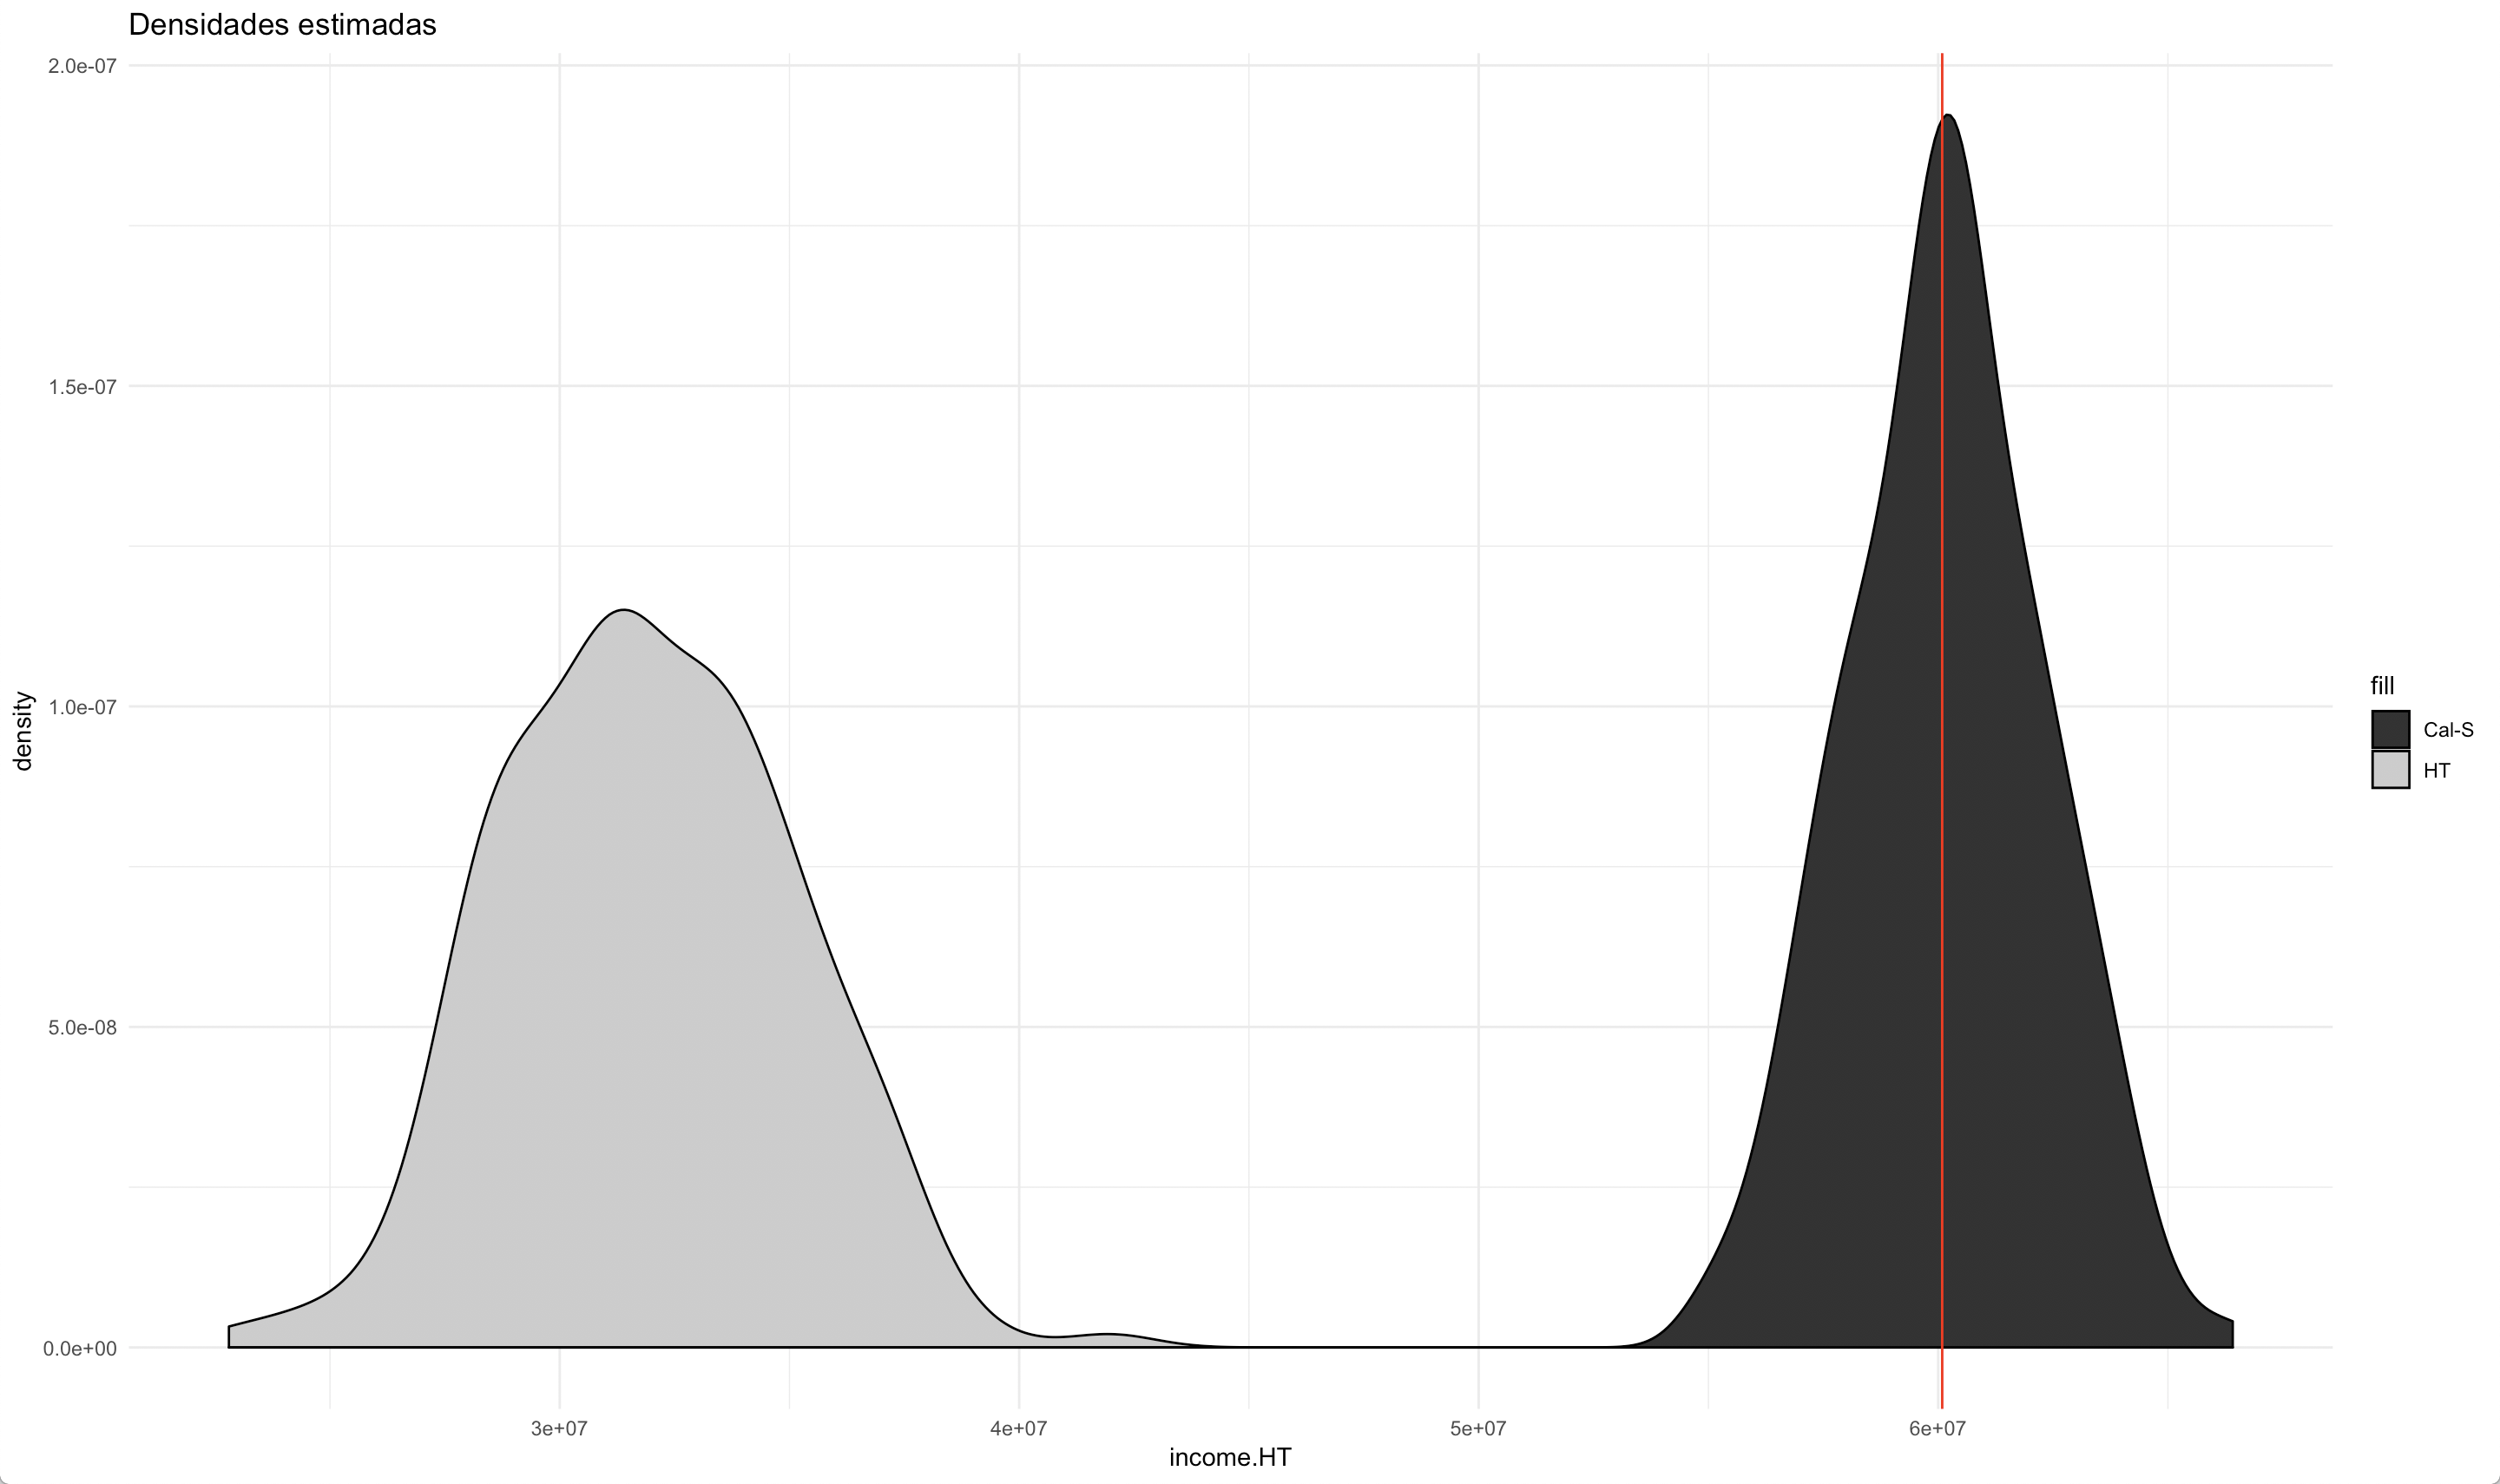
\includegraphics[width=0.5\linewidth]{Pics/c10} 

}

\caption{Distribuciones del estimador de Horvtiz-Thompson y del estimador de calibración}\label{fig:fightcaldist}
\end{figure}

Como se mencionó anteriormente, hay mejores formas de calibrar, puesto que el problema de la calibración se reduce a cómo introducir la información auxiliar en la estructura de estimación de la encuesta, es posible que existan variables que reduzcan el sesgo, pero no todas las variables inducirán el mismo nivel de precisión. Al momento de escoger, se deberían seleccionar aquellas variables que reduzcan el sesgo y que además reduzcan la varianza. Por tanto, las variables auxiliares que se usen como insumo en los procesos de calibración deben:

\begin{itemize}
\tightlist
\item
  Ser capaces de explicar la variación de la probabilidad de respuesta.
\item
  Estar correlacionadas con las variables de interés.
\item
  Identificar los dominios de estimación más importantes.
\end{itemize}

En particular al introducir otras covariables en la calibración (grupo de edad, escolaridad, región, área), además de la corrección del sesgo se evidencia un aumento de la precisión en las nuevas estimaciones, tal como lo muestra las distribuciones de los estimadores en la figura \ref{fig:fightcal2dist}, en donde se consideran tres estimadores: el estimador de Horvitz-Thompson (gris claro), el estimador de calibración con restricción de sexo (negro) y el estimador de calibración con todas las restricciones (gris oscuro).

\begin{figure}

{\centering 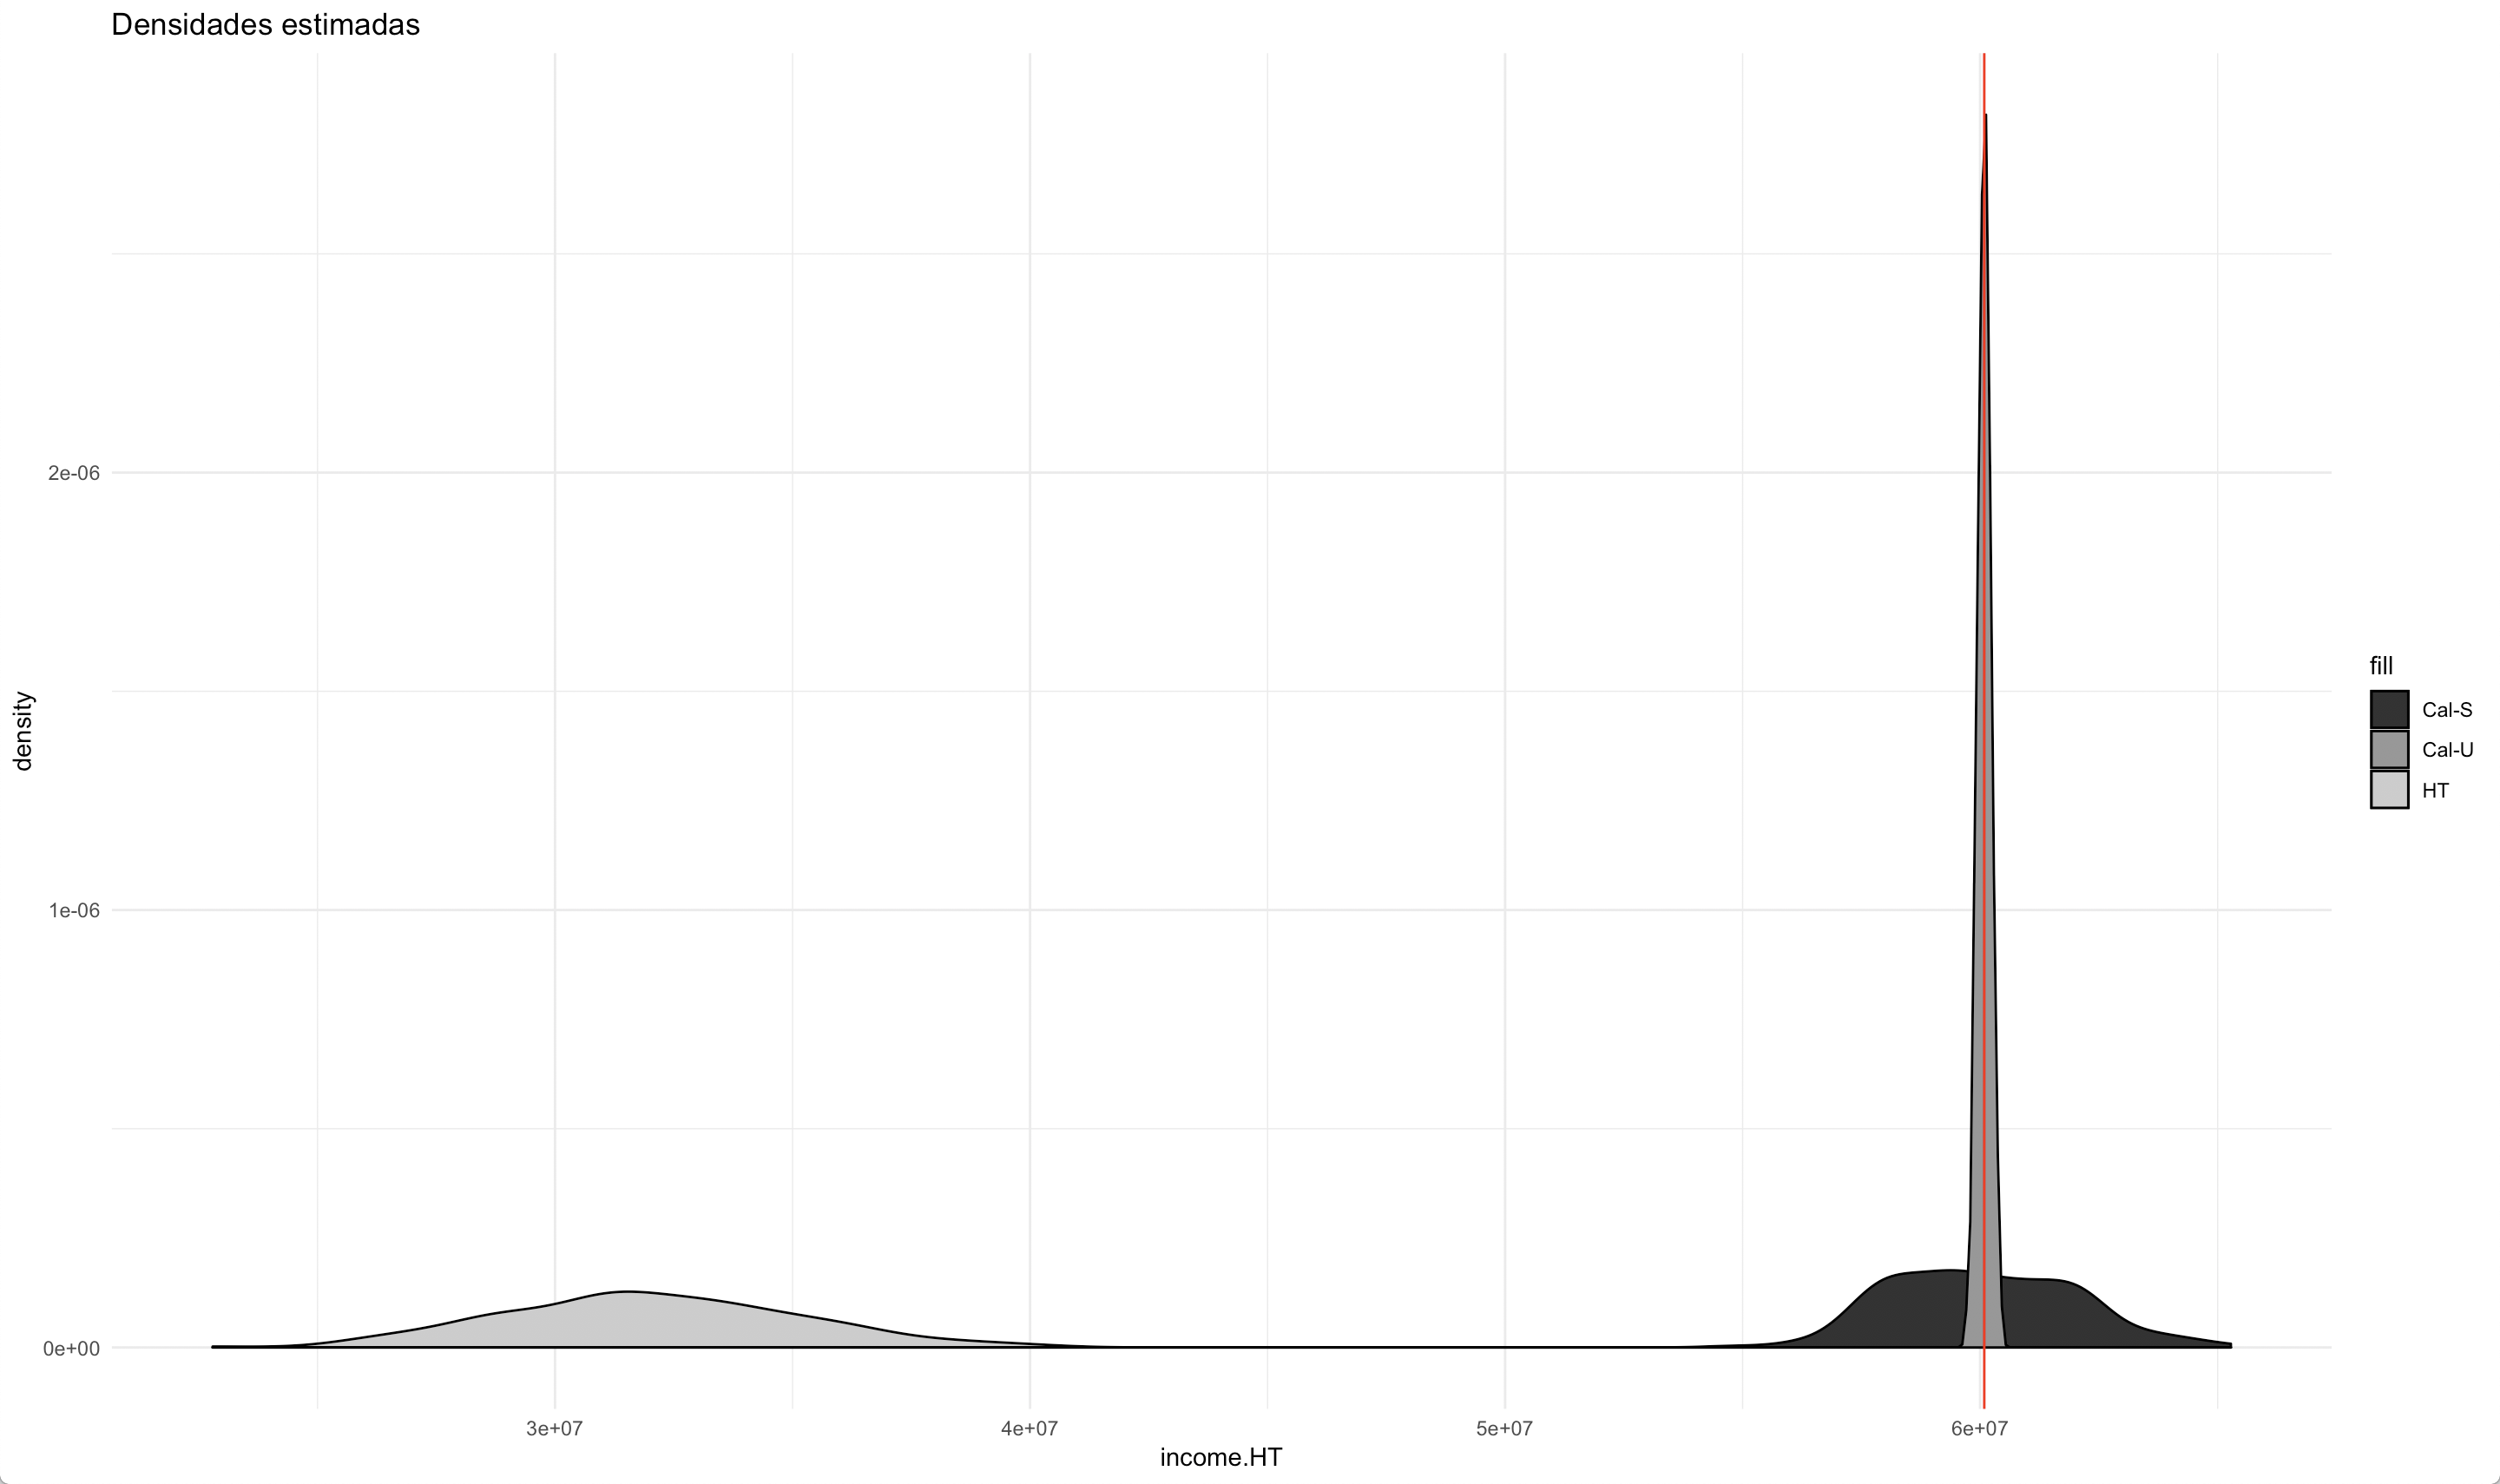
\includegraphics[width=0.5\linewidth]{Pics/c12} 

}

\caption{Distribuciones del estimador de Horvtiz-Thompson y de dos estimadores de calibración}\label{fig:fightcal2dist}
\end{figure}

\hypertarget{las-consecuencias-de-la-pandemia-por-covid-19-en-las-encuestas-de-la-regiuxf3n}{%
\section{Las consecuencias de la pandemia por COVID-19 en las encuestas de la región}\label{las-consecuencias-de-la-pandemia-por-covid-19-en-las-encuestas-de-la-regiuxf3n}}

Siguiendo a \citet{CEPAL_sesgos2020}, en su intento por frenar la velocidad de contagio del COVID-19, los gobiernos de la región determinaron la imposición de restricciones de movilidad que truncaron la recolección presencial de las encuestas de hogares. Para hacer frente a este inconveniente y poder seguir produciendo estadísticas oficiales pertinentes y oportunas, la mayoría de INE en la región decidieron realizar el seguimiento continuo a un panel seleccionado de un periodo reciente y mediante contacto telefónico seguir con la recolección de la información primaria. Uno de los retos más importantes que esta pandemia le impuso a los INE fue la corrección del sesgo de selección en las encuestas de hogares. A pesar de los ingentes esfuerzos que se hicieron por minimizarlo durante la recolección, el cambio de un modo presencial a un modo telefónico trajo consigo consecuencias indeseadas que se pudieron enfrentar con algunas de las metodologías que se explicaron en esta sección.

En \citet{CEPAL_publica}, se afirma que un buen punto de partida para los INE fue poder contar con una muestra probabilística de meses anteriores y conformar con ella un panel de seguimiento durante el periodo en el que se tuvieron estas restricciones de movilidad. En términos de notación, llamémosla la muestra maestra. Sin embargo, se debe tener en cuenta los siguientes dos aspectos importantes:

\begin{enumerate}
\def\labelenumi{\arabic{enumi}.}
\tightlist
\item
  No todos los hogares seleccionados de forma probabilística proveyeron su información de contacto telefónico.
\item
  No todos los hogares contactables respondieron el cuestionario de la encuesta.
\end{enumerate}

Haciendo cálculos gruesos, si suponemos que la cobertura de la submuestra que sí proveyó datos de contacto asciende al 85 \% y que la probabilidad de que un hogar contactado responda toda la encuesta es del 80 \%, entonces contaríamos solamente con un 68\% de la muestra original. A estas cuentas habría que ajustarlas con el efecto de la atrición en el panel, que crece a medida que se siga utilizando. En estos términos, sería un grave error y una suposición poco plausible asumir que los hogares respondientes efectivos se comportan de manera similar a los hogares no respondientes y a los hogares no cubiertos. El mejor escenario que puede plantearse es considerar que la muestra efectiva no está libre de sesgos, hacer una búsqueda exploratoria de su magnitud con los datos recolectados y tratar de minimizarlo (o incluso eliminarlo) utilizando alguna de las técnicas estadísticas que mencionamos en este documento.

La figura \ref{fig:fight3dist} presenta tres posibles escenarios que los INE pudieron encontrar en esta búsqueda. En el diagrama de la izquierda se verifica la ausencia de sesgo, en el diagrama del centro y en el de la derecha se confirma que la magnitud del sesgo es significativa. Nótese que la línea horizontal azul correspondería a la estimación publicada en el mes en el que se seleccionó la muestra maestra, mientras que la línea roja horizontal representa el promedio de las simulaciones con la muestra efectiva. Cada uno de los resultados de las simulaciones está representado por las fluctuaciones punteadas.

\begin{figure}

{\centering 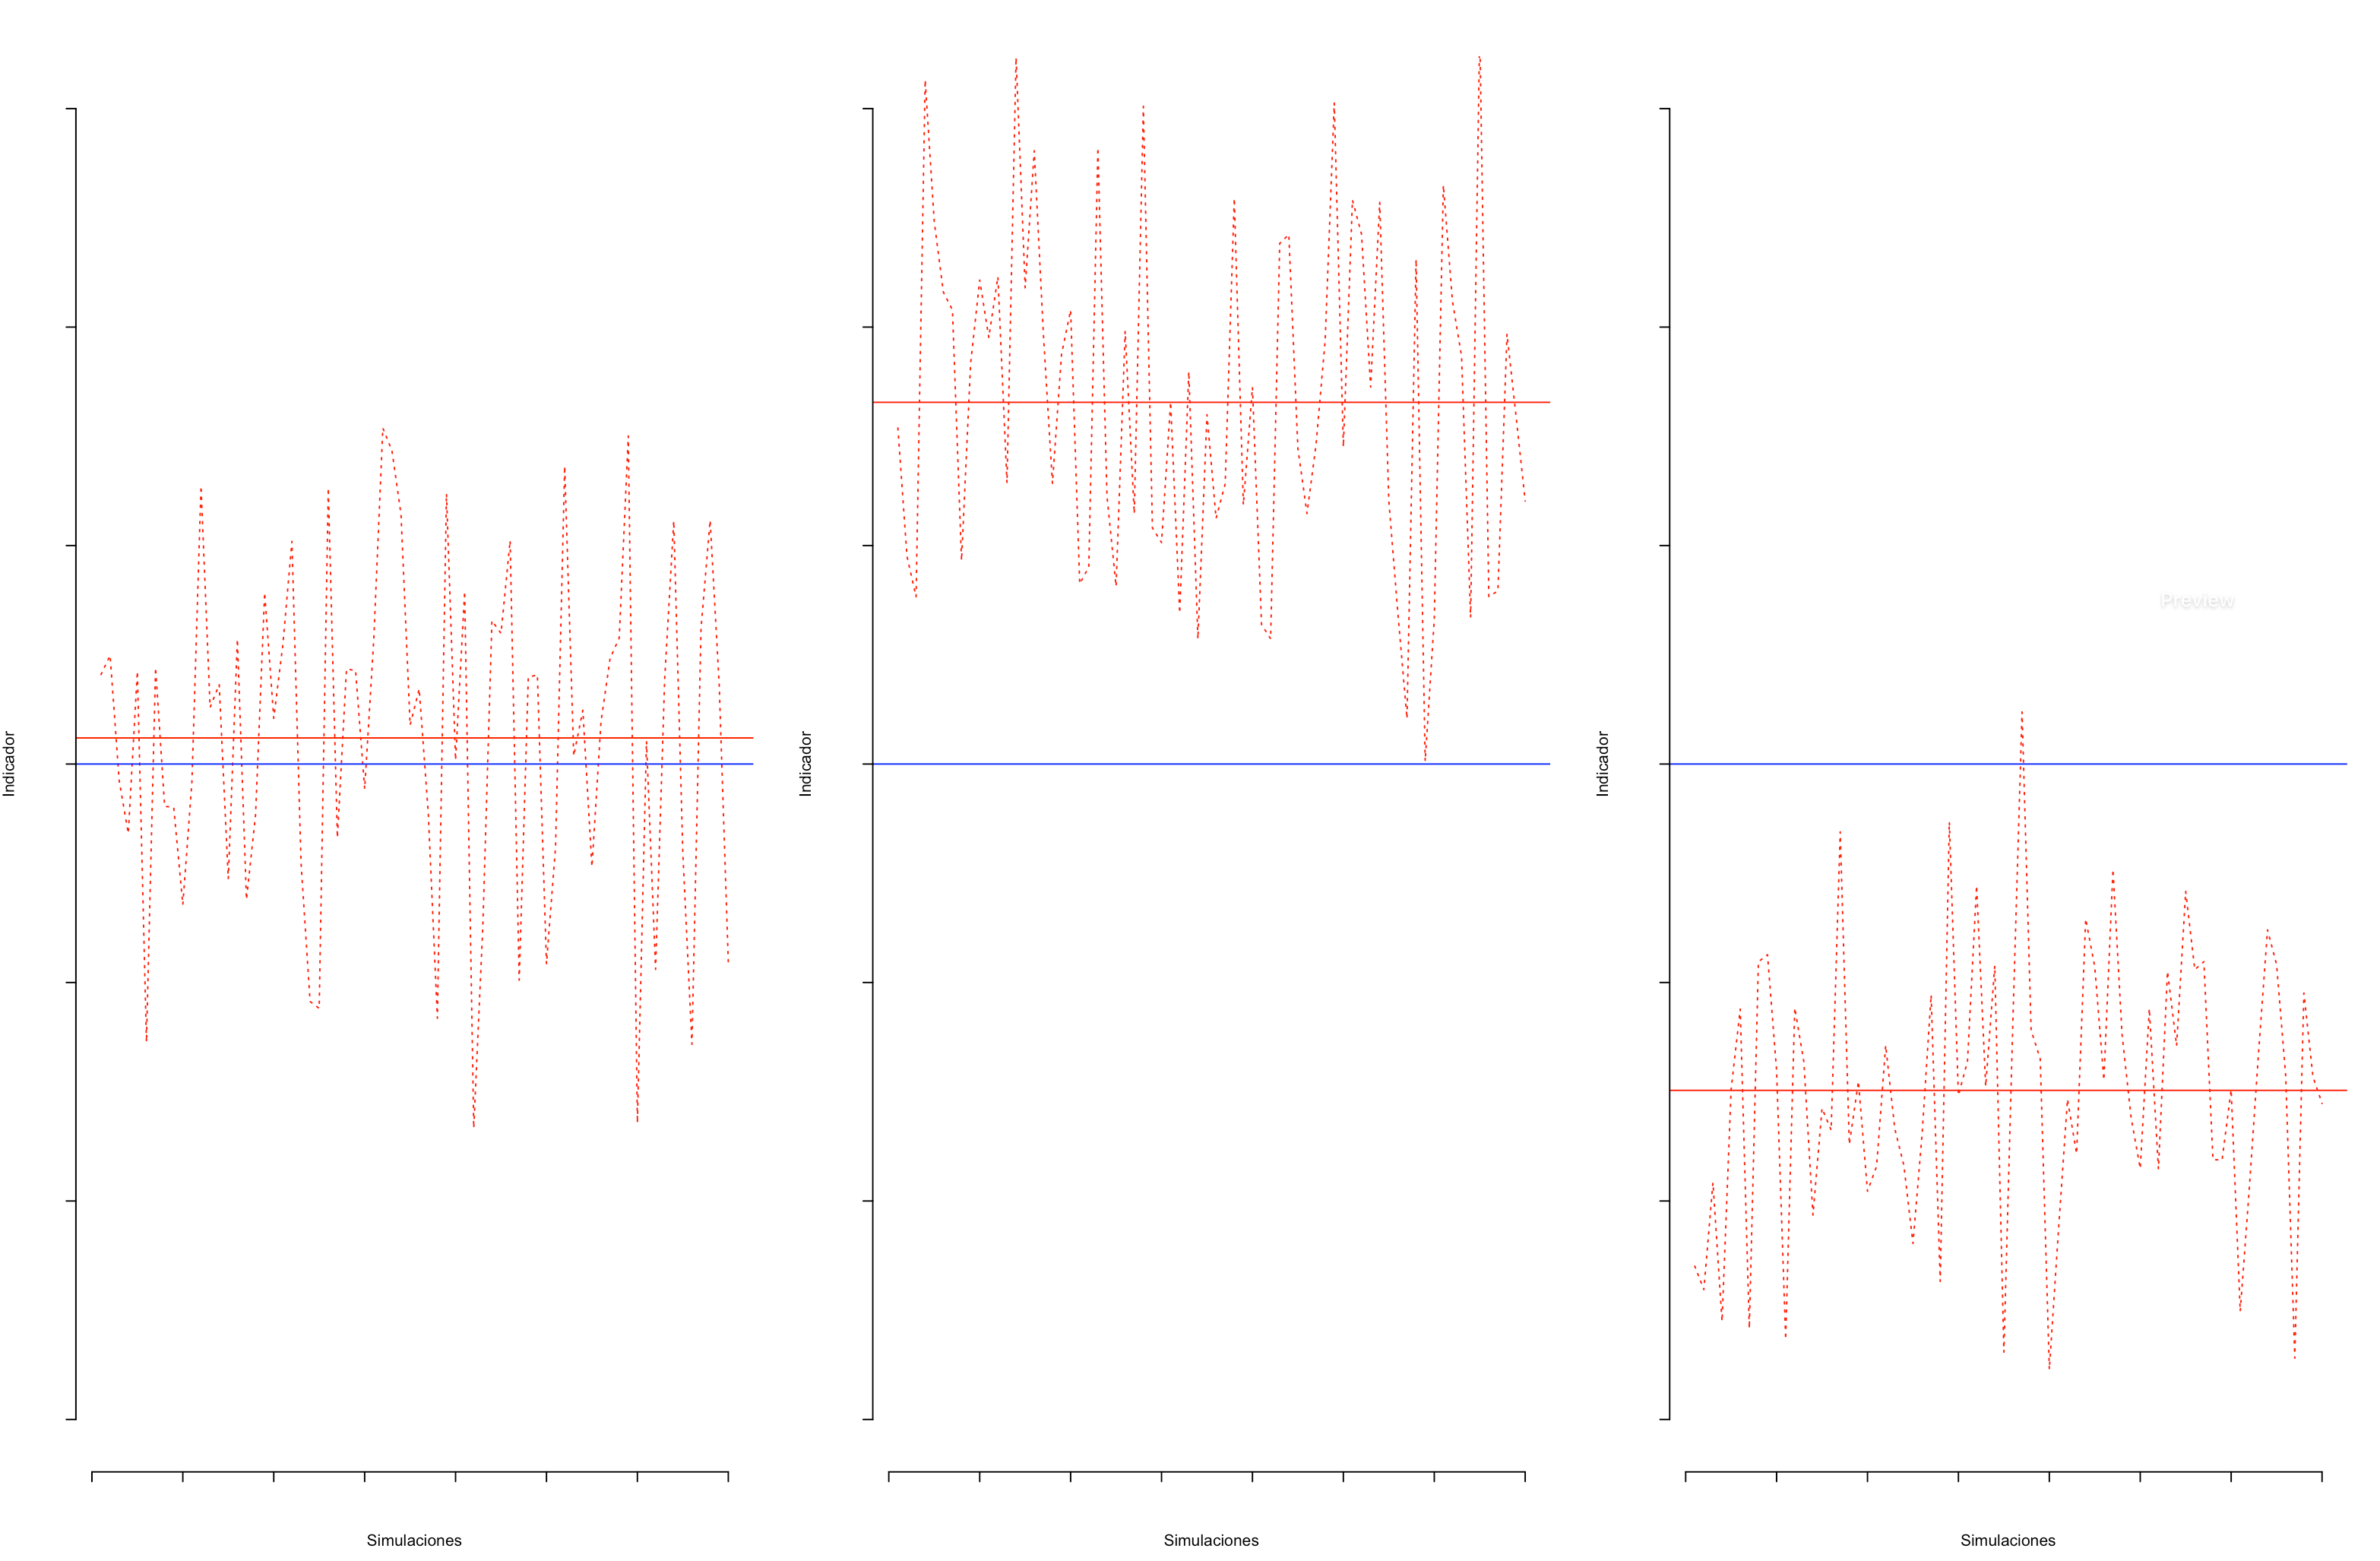
\includegraphics[width=0.5\linewidth]{Pics/calnr1} 

}

\caption{Distribuciones del estimador de Horvtiz-Thompson en tres escenarios de interés.}\label{fig:fight3dist}
\end{figure}

La figura \ref{fig:fight4dist} muestra un escenario simulado en donde se contempla el uso del estimador ajustado con la técnica de \emph{propensity score} (línea verde) y el estimador de calibración en dos etapas (línea azul) comparado con el estimador sin ningún tipo de ajuste (línea negra). Lo que se esperaría es que es estimador ingenuo subestime los tamaños poblacionales y los indicadores de interés; mientras que los estimadores ajustados, siempre que el mecanismo de ausencia de respuesta sea MAR o MCAR, elimina este sesgo.

\begin{figure}

{\centering 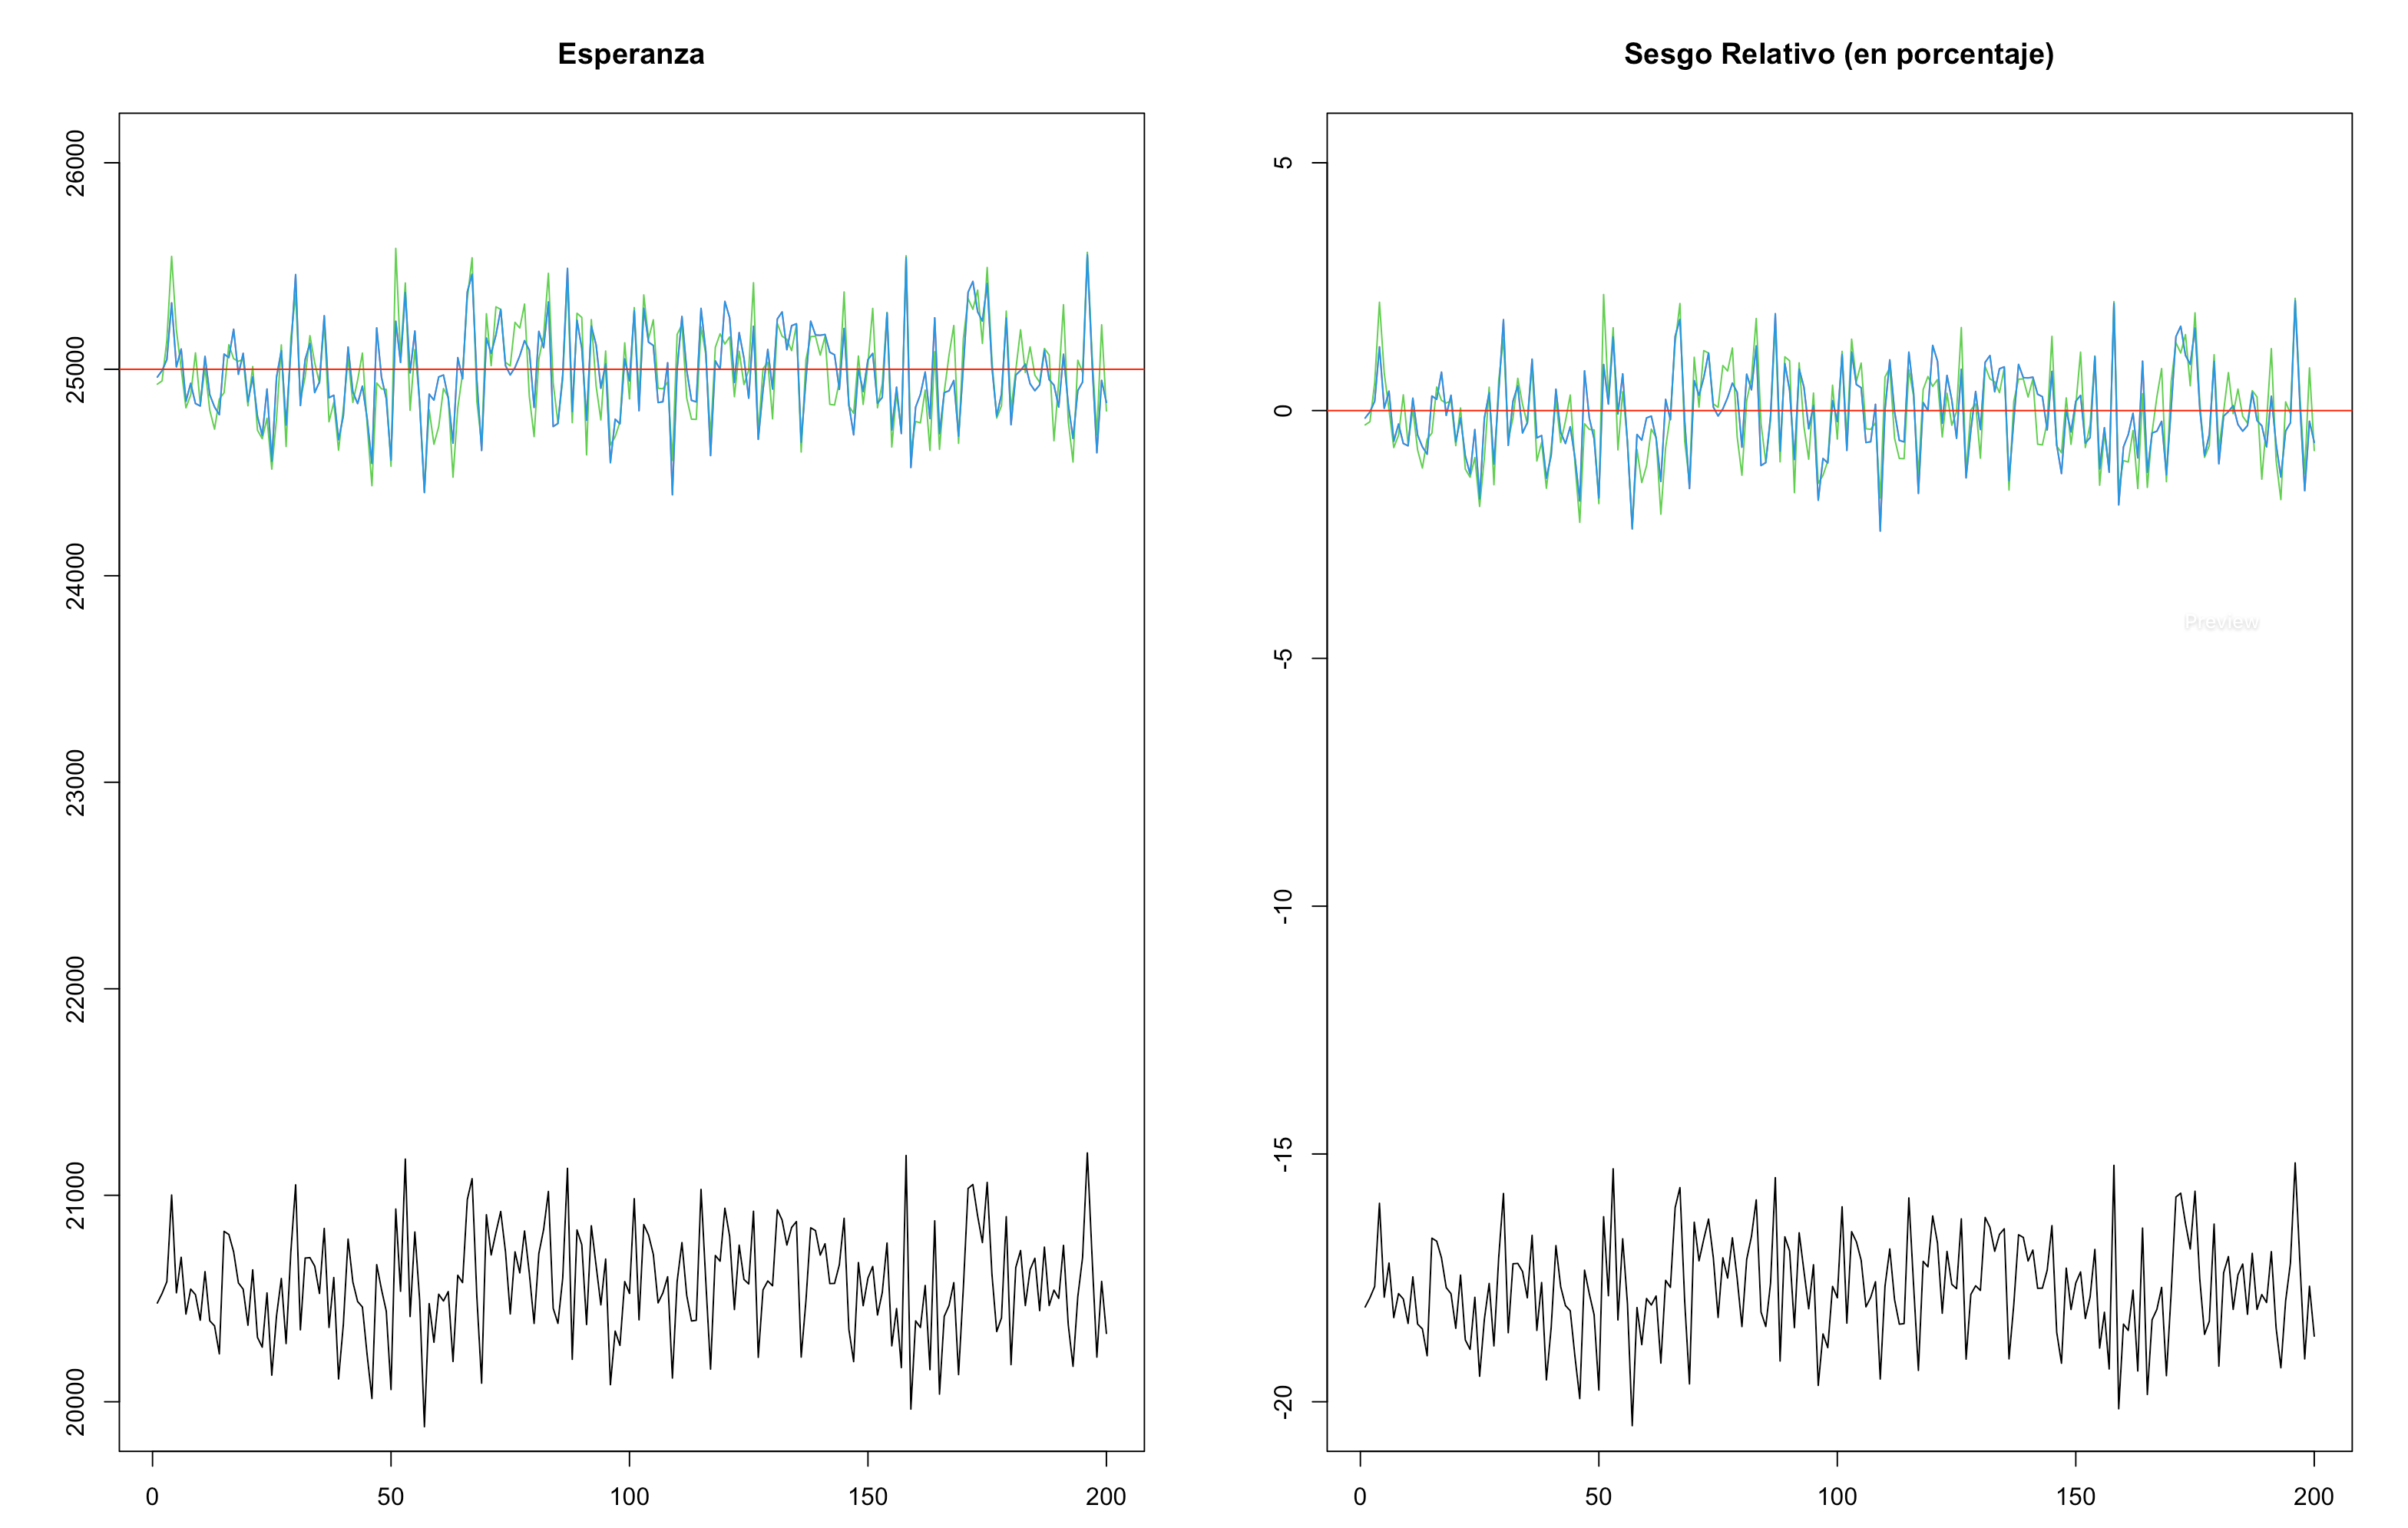
\includegraphics[width=0.5\linewidth]{Pics/calnr2} 

}

\caption{Distribuciones del estimador de Horvtiz-Thompson y de dos estimadores ajustados.}\label{fig:fight4dist}
\end{figure}

Los caminos que se deben seguir luego de corroborar la presencia (o ausencia) de sesgo dependerán de la estrategia de levantamiento de información que los países hayan decidido hacer. En el escenario más optimista, ante la ausencia de sesgo, se estaría en una buena posición para replicar los procesos usuales de inferencia. Sin embargo, ante la sospecha de que sí existe sesgo - posición parsimoniosa y recomendada por \citet{CEPAL_sesgos2020} -, y dependiendo de la información auxiliar disponible, los INE pudieron disponer de las dos alternativas metodológicas que se describieron anteriormente.

Muchos países de la región decidieron realizar un seguimiento mensual telefónico a la muestra maestra como alternativa a las restricciones de movilidad que se han impuesto en los países y que impiden la recolección presencial de la información. En este caso, partiendo de una muestra probabilística se pueden realizar ajustes a los factores de expansión de manera diferencial \citep{CEPAL_continua}.

En particular, dado que se tuvo acceso a todo un conjunto de covariables \(\mathbf{x}\) en la muestra maestra, fue posible determinar el mejor modelo para estimar el patrón de ausencia de respuesta en la muestra de respondientes efectivos. En este paso se asumió que la probabilidad de respuesta dependía de alguna combinación lineal de las covariables en la muestra maestra; es decir que el mecanismo que genera esa ausencia de respuesta se pudo describir mediante \(\mathbf{x}\). Teniendo en cuenta que los pesos originales de la encuesta telefónica se denotan como \(d_k\), y habiendo estimado \(\hat\phi_{k}\) para respondientes y no respondientes de la muestra telefónica, entonces el factor de expansión ajustado tomó forma \(w_k = \frac{d_k}{\hat{\phi}_k}\).

En este sentido, utilizar el factor de expansión \(w_k\) minimizaría el sesgo de selección que se generó por el cambio de modo en la recolección de la información. Por ejemplo, podría considerarse que un buen modelo de \emph{propensity score} contemplase la edad, el nivel educativo, el área de residencia (rural/urbano), el sexo del respondiente, la región geográfica, el estado de ocupación en el mes de observación de la muestra maestra y el ingreso percápita del hogar. Nótese que todas las covariables en el modelo, salvo el área y la región geográfica, necesariamente provienen de las observaciones obtenidas en la muestra maestra.

Por otro lado, \citet{CEPAL_publica} afirma que al imponer una cierta coherencia entre las cifras oficiales ya publicadas y las que la encuesta telefónica pudo producir, es preferible el uso de los estimadores de calibración. Al usar este enfoque se asegura una estructura inferencial robusta en presencia de la información disponible puesto que se reduce tanto el error de muestreo (aumentando la precisión) como el error debido a la ausencia de respuesta (eliminando el sesgo). A manera de ejemplo, podríamos considerar que las siguientes dos etapas de la calibración son suficientes para eliminar el sesgo generado por el cambio de modo de recolección:

\begin{itemize}
\tightlist
\item
  En la primera etapa se calibran los pesos de la muestra maestra usando las variables de edad, región, área y sexo, definidas convenientemente en \(\boldsymbol{x}_{1k}\). Los totales de estas variables se encuentran en los conteos censales o en su defecto, en las proyecciones demográficas.
\item
  En una segunda etapa se calibrarán los pesos de la muestra telefónica usando las anteriores variables \(\boldsymbol{x}_{1k}\) y además las variables de ingreso percápita, condición de ocupación, rama de actividad y escolaridad, definidas convenientemente en en \(\boldsymbol{x}_{2k}\). Los totales de estas variables fueron estimados en la misma publicación de la encuesta basada en la muestra maestra.
\end{itemize}

\hypertarget{ejemplo}{%
\subsection{Ejemplo}\label{ejemplo}}

Esta sección revisa los pasos principales que se debieron considerar para erradicar (o al menos minimizar en la medida más considerable) el sesgo de selección de una encuesta recopilada durante la pandemia por COVID19. Los datos que se usarán son artificiales, pero sirven para mostrar y ejemplificar las diferentes etapas propuestas para la evaluación y minimización del impacto del COVID-19 en la calidad de las encuestas.

Supongamos un conjunto de datos artificial que define una población finita \(U\) de tamaño \(N = 50000\), y supongamos que estamos interesados en observar la situación laboral de cada persona en \(U\). En aras de la simplicidad, supondremos que una persona solo puede estar \emph{empleada} o \emph{desempleada}. Quisiéramos observar esta característica de interés en dos periodos diferentes \(t_0\) y \(t_1\). Por un lado, suponga que \(t_0\) corresponde a un período de recolección regular antes de la pandemia; por otro lado, supongamos que \(t_1\) corresponde al período donde las restricciones de movimiento debido a la pandemia afectaron la recolección estándar de encuestas por muestreo.

Si tuviéramos acceso a toda la población, nos encontraríamos con que en \(t_0\), el 80\% de las personas estaría empleada, mientras que el 20\% estaría desempleada. Sin embargo, debido al impacto de la pandemia en los indicadores sociales (e.g., pobreza y mercado laboral), en \(t_1\), observaríamos que muchas personas perdieron su trabajo, y la mitad de la población está desempleada.

El siguiente conjunto de datos en la tabla \ref{tab:tabsesgo1} muestra una versión reducida de los primeros 10 individuos de esta población finita.

\begin{table}

\caption{\label{tab:tabsesgo1}Un vistazo a la población del ejemplo. 10 primeras filas de un total de 50000.}
\centering
\begin{tabular}[t]{l|l}
\hline
y0 & y1\\
\hline
Ocupado & Ocupado\\
\hline
Ocupado & Desocupado\\
\hline
Ocupado & Ocupado\\
\hline
Ocupado & Ocupado\\
\hline
Ocupado & Desocupado\\
\hline
Ocupado & Desocupado\\
\hline
Ocupado & Ocupado\\
\hline
Desocupado & Desocupado\\
\hline
Ocupado & Desocupado\\
\hline
Ocupado & Desocupado\\
\hline
\end{tabular}
\end{table}

Las tablas \ref{tab:tabsesgo2} y \ref{tab:tabsesgo3} muestran los flujos netos de la población finita en los dos períodos considerados. Tenga en cuenta que \(y_0\) representa la característica de interés en el período previo a la pandemia; mientras tanto, \(y_1\) representa la característica de interés en el período de la pandemia por COVID-19.

\begin{table}

\caption{\label{tab:tabsesgo2}Flujos netos verdaderos en la población del ejemplo antes de la pandemia por COVID-19}
\centering
\begin{tabular}[t]{l|r|r}
\hline
y0 & n & prop\\
\hline
Desocupado & 10000 & 0.2\\
\hline
Ocupado & 40000 & 0.8\\
\hline
\end{tabular}
\end{table}

\begin{table}

\caption{\label{tab:tabsesgo3}Flujos netos verdaderos en la población del ejemplo en medio de la pandemia por COVID-19}
\centering
\begin{tabular}[t]{l|r|r}
\hline
y1 & n & prop\\
\hline
Desocupado & 25000 & 0.5\\
\hline
Ocupado & 25000 & 0.5\\
\hline
\end{tabular}
\end{table}

La tabla \ref{tab:tabsesgo4} muestra los flujos brutos de la población finita entre los dos periodos considerados. Como se puede observar, 25000 personas permanecieron ocupadas en los dos periodos, y 15000 personas cambiaron su situación laboral de ocupadas a desocupadas; de los desempleados en el primer período, ninguno pudo conseguir trabajo, mientras que 10000 personas permanecieron desempleadas en ambos períodos.

\begin{table}

\caption{\label{tab:tabsesgo4}Flujos brutos verdaderos del cambio en el estado laboral en la población de ejemplo.}
\centering
\begin{tabular}[t]{l|r|r}
\hline
y0 & Desocupado & Ocupado\\
\hline
Desocupado & 10000 & 0\\
\hline
Ocupado & 15000 & 25000\\
\hline
\end{tabular}
\end{table}

La medición y observación de la situación laboral se realiza a través de una encuesta por muestreo en ambos períodos. De esta forma, supongamos que se selecciona una muestra aleatoria simple sin reemplazo \(s_0\) de tamaño \(n_0 = 4000\) de \(U\). Para simplificar, supongamos que se pretende observar la misma muestra en ambos períodos (tipo panel).

Como el lector debe considerar, la muestra anterior a la pandemia tenía un modo regular de recolección presencial. Sin embargo, dadas las restricciones de movilidad impuestas por los gobiernos para frenar la propagación de la pandemia, la modalidad de recolección del último período debió cambiar. Los INE usaron los registros de la muestra anterior (antes del COVID-19) para obtener el número de teléfono de los hogares seleccionados, tratar de hacer un contacto exitoso y administrar un cuestionario por teléfono. Por supuesto, las tasas de muestreo en ambos períodos diferirían, puesto que no todos los hogares de la primera muestra proporcionaron un número de teléfono válido y, de los válidos, no todos contestaron la encuesta telefónica.

La muestra telefónica es más pequeña (2305) que la muestra realizada cara a cara (4000). Los investigadores sospechan que los sesgos de selección no son despreciables en la muestra telefónica. Las tablas \ref{tab:tabsesgo5} y \ref{tab:tabsesgo6} muestran los resultados basados en las muestras (no ponderados) para la encuesta cara a cara y la encuesta telefónica, respectivamente.

\begin{table}

\caption{\label{tab:tabsesgo5}Resultados observados en la muestra presencial del ejemplo.}
\centering
\begin{tabular}[t]{l|l|r|r}
\hline
  & Estado & n & prop\\
\hline
Desocupado & Desocupado & 820 & 0.205\\
\hline
Ocupado & Ocupado & 3180 & 0.795\\
\hline
\end{tabular}
\end{table}

\begin{table}

\caption{\label{tab:tabsesgo6}Resultados observados en la muestra telefónica del ejemplo.}
\centering
\begin{tabular}[t]{l|l|r|r}
\hline
  & Estado & n & prop\\
\hline
Desocupado & Desocupado & 909 & 0.3943601\\
\hline
Ocupado & Ocupado & 1396 & 0.6056399\\
\hline
\end{tabular}
\end{table}

El primer paso en la búsqueda de sesgos de selección es calcular la tasa de respuesta. En este caso, de 4000 encuestados seleccionados originalmente, solo 2305 respondió a la entrevista telefónica. Lo que equivale a una tasa de respuesta de tan solo el 58 \%.

Luego, se debe evaluar la naturaleza de la ausencia de repuesta. Este paso está dedicado a reconocer si la falta de respuesta sigue una estructura MAR o MCAR. Bajo el supuesto MCAR, uno no esperaría encontrar patrones fuertes en las covariables; es decir, ninguna categoría dentro de las covariables debe mostrar una tasa de respuesta diferente. Por otro lado, bajo el supuesto MAR, uno puede encontrar patrones fuertes en una o múltiples covariables. Para verificar qué supuesto (MAR o MCAR) se ajusta mejor a las observaciones de la muestra seleccionada durante el COVID19, supongamos que sí tenemos acceso a los datos de la muestra de la muestra pre-pandemia y podemos identificar a los individuos, encuestados y no encuestados, de la última muestra.

Como se ve en la tabla \ref{tab:tabsesgo7}, de los 2305 encuestados en la encuesta telefónica, 3.8177874\% estaban empleados en el período anterior, y aproximadamente 96.1822126\% estaban desempleados, lo que podría ser indicio de un patrón de ausencia de respuesta MAR.

\begin{table}

\caption{\label{tab:tabsesgo7}Proporción observada del estado de ocupación en la muestra telefónica del ejemplo. }
\centering
\begin{tabular}[t]{l|l|r|r}
\hline
  & Estado & n & prop\\
\hline
Desocupado & Desocupado & 88 & 0.0381779\\
\hline
Ocupado & Ocupado & 2217 & 0.9618221\\
\hline
\end{tabular}
\end{table}

Finalmente, de la tabla \ref{tab:tabsesgo8}, se deduce que al examinar el estado anterior, de los 1695 no encuestados, se observa que casi el 43.1858407\% estaban empleados en el periodo anterior, mientras que el 56.8141593\% estaban desempleados. Las proporciones no son similares en ningún aspecto, lo que apunta a un posible sesgo de selección.

\begin{table}

\caption{\label{tab:tabsesgo8}Proporción observada del estado de ocupación en la muestra telefónica del ejemplo.}
\centering
\begin{tabular}[t]{l|l|r|r}
\hline
  & Estado & n & prop\\
\hline
Desocupado & Desocupado & 732 & 0.4318584\\
\hline
Ocupado & Ocupado & 963 & 0.5681416\\
\hline
\end{tabular}
\end{table}

Para verificar la asociación entre la respuesta en la encuesta telefónica y la situación laboral en la encuesta presencial, se puede utilizar herramientas de inferencia clásica, como la estadística Ji-cuadrado de Pearson y el estadístico V de Cramer. La tabla \ref{tab:tabsesgo9} resume el comportamiento de la respuesta en la encuesta telefónica dada la situación laboral en la encuesta presencial.

\begin{table}

\caption{\label{tab:tabsesgo9}Asociación entre la respuesta telefónica y el estado de ocupación en el periodo anterior en la muestra del ejemplo.}
\centering
\begin{tabular}[t]{l|l|r}
\hline
Estado & Respuesta & Freq\\
\hline
Desocupado & 0 & 732\\
\hline
Ocupado & 0 & 963\\
\hline
Desocupado & 1 & 88\\
\hline
Ocupado & 1 & 2217\\
\hline
\end{tabular}
\end{table}

Basado en la información provista por la tabla anterior, es posible realizar la prueba de bondad de ajuste de Pearson entre las dos variables de interés (respuesta en la encuesta telefónica y situación laboral en la encuesta presencial) para determinar si existe una correlación significativa. El sistema de hipótesis es el siguiente:

\begin{itemize}
\tightlist
\item
  H0: Las dos variables son independientes.
\item
  H1: Las dos variables se relacionan entre sí.
\end{itemize}

A partir de estos datos, la estadística de prueba toma el valor de 944 (muy grande) con un valor-p muy pequeño y cercano a cero, lo que indica una fuerte relación. Finalmente, la estadística V de Cramer mide la fuerza de la asociación entre dos variables nominales, y toma valores entre cero (sin asociación) y uno (asociación fuerte). Para este caso, el valor del estadístico es cercano a 0,5, indicando una asociación significativa que debe ser considerada en los próximos pasos para minimizar el posible sesgo de selección que puede afectar la inferencia de la encuesta telefónica.

Como se pudo observar anteriormente, existe fuerte evidencia de que el mecanismo de respuesta de la encuesta telefónica depende de la situación laboral del individuo en el período anterior. Eso significa que las personas que estaban desempleadas tienden a responder menos que las personas que estaban empleadas. Para simplificar el ejemplo, asumimos que la probabilidad de ser un encuestado depende de la situación laboral anterior. De esta forma, \(\phi_k\) puede escribirse como una función de ese estado laboral anterior, incluido en las covariables \(\mathbf{z}\).

\[
{\phi}_k = f(\mathbf{z}_k, {\boldsymbol{\beta}})   
\]

Como \(\phi_k\) se puede escribir como una función de las covariables disponibles, podemos afirmar que el mecanismo de respuesta sigue un enfoque MAR. Como el patrón de no respuesta es MAR, y es posible tener acceso a las covariables \(\mathbf{z}\) que determinan el mecanismo de respuesta, entonces también será posible estimar las probabilidades de respuesta por \(\hat{\phi}_k = f(\mathbf{z }_k, \hat{\boldsymbol{\beta}})\) para usarlo en la generación de nuevos pesos. Después de ajustar un modelo de \emph{propensity-score}, la figura \ref{fig:figsesgo1} muestra el histograma de laas probabilidades de respuesta estimadas, las cuales solo toman dos valores (0.6971698 y 0.1073171 ), uno para cada categoría de la situación laboral en la encuesta presencial.

\begin{figure}

{\centering 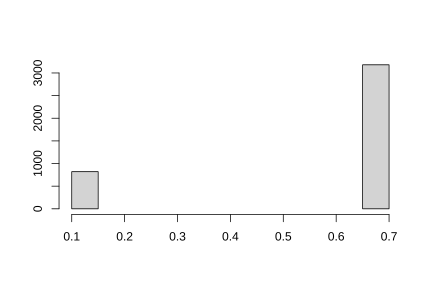
\includegraphics{13SesgoUnidad_files/figure-latex/figsesgo1-1} 

}

\caption{Histograma de los *propensity-score*}\label{fig:figsesgo1}
\end{figure}

Luego, utilizando los datos telefónicos y el nuevo conjunto de ponderaciones \(d_{4k}\), ajustado por el puntaje de propensión estimado, tenemos que el número estimado de empleados en el período COVID es \(\hat{t}_y=\sum_{k\in s_{ER}}d_{4k}y_{1k} =\) 24970.23.

Por otra parte, también es posible calibrar los pesos en la muestra telefónica a nivel de la información auxiliar disponible en la muestra presencial, y luego a nivel nacional. Como el mecanismo que genera la falta de respuesta es MAR, es posible que este nuevo conjunto de pesos de calibración elimine el sesgo. Para lograr este objetivo, se encuentra un primer conjunto de pesos calibrados sujetos a la siguiente restricción:

\[
\sum_{s_0}w_{0k}\boldsymbol{x}_{k} = \sum_{U}\boldsymbol{x}_{k} = \mathbf{t_x}
\]

Donde \(\mathbf{t_x}\) puede representar conteos nacionales provenientes de censos o proyecciones demográficas. Luego, en una segunda etapa, estos pesos intermedios \(w_{0k}\) deben utilizarse para calcular los pesos finales de calibración \(w_{1k}\) de la muestra de encuestados efectivos que están sujetos a la siguiente restricción:

\[
\sum_{s_0}w_{1k}\boldsymbol{x}_{k} =
\begin{pmatrix}
\sum_{U}\boldsymbol{x}_{k}\\
\sum_{s_1}w_{0k}\boldsymbol{z}_{k} 
\end{pmatrix} =
\begin{pmatrix}
\mathbf{t_x}\\
\hat{\mathbf{t}}_\mathbf{z}
\end{pmatrix}
\]

En donde, \(\hat{\mathbf{t}}_\mathbf{z}\) representa las cifras estimadas provenientes de la encuesta presencial. El estimador de calibración se puede escribir de la siguiente manera:

\[
\hat{t}_y^{cal}=\sum_{k\in s_1}w_{1k}y_{1k}
\]

Después de realizar la calibración en dos etapas, y utilizando los datos de la encuestas telefónica junto con el nuevo conjunto de pesos calibradas, tenemos que el número estimado de empleados en el período COVID es \(\hat{t}_y^{cal}=\sum_{k\in s_1}w_{1k}y_{1k}=\) \texttt{format\ r(Tyhat.cal,\ scientific\ =\ F)}. Tenga en cuenta que la forma funcional de los pesos de calibración doble resultantes de este proceso de optimización se pueden escribir de la siguiente manera:

\[
w_{1k} = d_k \times g_{0k} \times g_{1k} \cong d_k \times \hat \phi_k
\]

Por lo tanto, bajo este escenario, los pesos \(g_k\) pueden verse como una estimación de las probabilidades de respuesta \(\phi_k\). La figura \ref{fig:figsesgo2} muestra el histograma de los puntajes de propensión pronosticados. Solo toman dos valores (0.6928125 y 0.11 ), uno para cada categoría del estatus laboral en la encuesta cara a cara.

\begin{figure}

{\centering 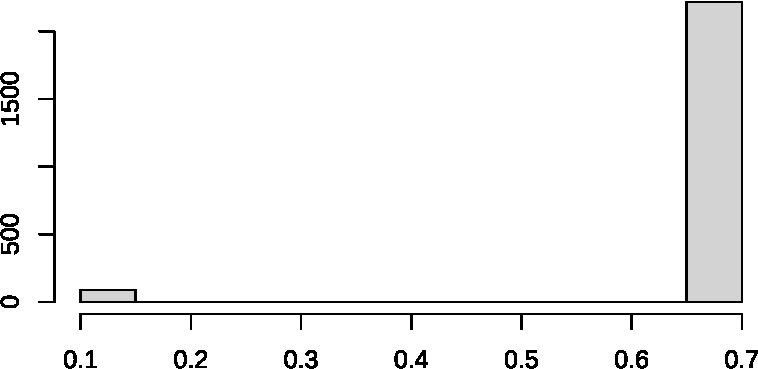
\includegraphics{13SesgoUnidad_files/figure-latex/figsesgo2-1} 

}

\caption{Histograma de los pesos ajustados}\label{fig:figsesgo2}
\end{figure}

Por último, nótese que si no se considera el mecanismo de ausencia de respuesta, sería fácil obtener estimaciones engañosas y sesgadas. Este enfoque ingenuo e incorrecto conduce al siguiente estimador sesgado

\[
\hat{t}_y^{exp}=\sum_{k\in s_1}d_{3k}y_{1k}
\]

Donde \(d_{1k}\) se refiere a los pesos muestrales no ajustados de la encuesta telefónica. Bajo este escenario, el número estimado de empleados en el período COVID es \(\hat{t}_y^{exp}=\sum_{k\in s_1}d_{1k}y_{1k} =\) 19718.

\hypertarget{ausencia-de-respuesta-por-registro}{%
\chapter{Ausencia de respuesta por registro}\label{ausencia-de-respuesta-por-registro}}

En el diseño y puesta en marcha de una encuesta puede ocurrir cierto tipo de situaciones que pueden sesgar las estimaciones finales. Este tipo de sesgos puede ocurrir antes, durante y después de la recolección de los datos. Es tarea del estadístico advertir ante todas las posibles instancias de los problemas que causan los sesgos y procurar que, en todas las etapas de la encuesta, se minimice el error humano y el error estadístico para que al final los resultados del estudio sean tan confiables como sea posible.

Como se mencionó en los capítulos anteriores, el enfoque recomendado para hacer frente a la ausencia de respuesta es una combinación de los procedimientos de imputación y ponderación y se conoce como el \textbf{enfoque combinado}, el cual imputa los valores de las celdas vacías para los individuos que tienen al menos un registro faltante en la base de datos (exceptuando a aquellos que tienen todos o la mayoría de registros faltantes). En resumen, los individuos que no contestaron ninguna pregunta del cuestionario son eliminados del análisis, mientras que los restantes serán considerado en el análisis con sus respuestas originales o con la imputación de las celdas vacías.

En este capítulo se abordara el enfoque de la imputación utilizada para tratar la ausencia de respuesta por registro, y los posibles métodos que pueden utilizarse para identificar valores atípicos en la base de datos que, por consiguiente, pueden también ser imputados. Nótese que el verbo ``imputar'' viene del latín \emph{impute}, cuya traducción al español puede ser calcular, estimar o atribuir. En el siglo XIX se utilizó el término \textbf{ingreso imputado} para denotar el ingreso derivado de los bienes raíces. Según \citet{VanBuuren}, la connotación de la imputación, en el sentido de completar valores en una base de datos, aparece por primera vez en 1957 en el \emph{U.S. Census Bureau}. Es así como el tratamiento de datos faltantes consiste en \textbf{estimar} qué valores son \textbf{plausibles} para los datos faltantes, dados los demás valores en la base de datos.

\hypertarget{modelos-para-la-imputaciuxf3n}{%
\section{Modelos para la imputación}\label{modelos-para-la-imputaciuxf3n}}

El término imputación se refiere al conjunto de técnicas por las cuales los valores faltantes en una o más variables se reemplazan con información plausible con el objetivo de lograr valores sustitutivos en una base de datos que pueda ser analizada posteriormente. Este proceso introduce un nuevo elemento de error, conocido como el error de imputación, debido a la incertidumbre que introducen los valores no observados. Cuando se tiene ausencia de respuesta por registro, las técnicas de imputación se prefieren antes que la utilización de los esquemas de ponderación en la muestra. De esta manera, es posible crear un conjunto completo y rectangular de datos mediante la imputación de los valores faltantes, puesto que después de realizar la imputación, se espera que todos los valores del cuestionario de un individuo contengan información y no exista ningún vacío.

Para lograr la sustitución de los valores faltantes con información plausible, es posible encontrar donantes apropiados, en la misma muestra que se ha conseguido, definidos como respondientes que comparten características demográficas similares con el individuo que no respondió. Por lo tanto, la información del respondiente donante (o una función de estos valores) se copiará en las celdas vacías del no respondiente. Para encontrar los donantes es posible realizar un análisis estadístico con base en métodos de clasificación. Dentro de los métodos de imputación más usados en encuestas de hogares se encuentran los siguientes:

\begin{itemize}
\tightlist
\item
  Imputación promedio (\emph{mean value imputation}) que utiliza la media de la variable (dentro de las UPM o en un subconjunto apropiado de datos). En este caso, si se encuentra un valor faltante, inmediatamente será reemplazado por el promedio de los datos de los respondientes en un subgrupo apropiado.
\item
  Imputación por paquete caliente (\emph{hot deck imputation}) que reemplaza los valores faltantes por los valores de un donante que es un respondiente de la encuesta en el mismo levantamiento. En este caso, el valor faltante es reemplazado por la información del individuo escogido de antemano.
\item
  Imputación por paquete frío (\emph{cold deck imputation}) que reemplaza los valores faltantes por los valores de un donante que es un respondiente de la misma encuesta, pero en un levantamiento anterior. En este caso, el valor faltante es reemplazado por la información auxiliar de un individuo escogido de encuestas anteriores.
\item
  Imputación estadística basada en modelos estadísticos en donde la variable dependiente es aquella que se quiere imputar y las covariables se derivan del restante conjunto de datos. En este caso, el valor faltante es reemplazado por la predicción (o una función) del modelo ajustado con la información en la muestra.
\end{itemize}

Como se mencionó anteriormente, cuando se trata de imputación, se pueden definir dos tipos de métodos. La imputación de la unidad completa, que se produce cuando toda la información de un individuo es imputada, y la imputación de registros, que se da cuando los valores faltantes son imputados a nivel de los individuos. Observe que la imputación de la unidad se utiliza para hacerle frente a la ausencia de respuesta de la unidad, cuando no hay datos para el individuo, mientras que la imputación del registro se utiliza para la no respuesta del registro, cuando no todos los valores se proporcionan para un individuo, pero algunos sí.

La imputación se realiza a menudo en grupos no traslapados \(g= 1, \ldots, G\), donde la unión de \(s_1, \ldots, s_G\) equivale a la muestra completa \(s\). Se pueden utilizar diferentes métodos para cada grupo, pero dentro de cada grupo se debe utilizar el mismo método de imputación. Esto se debe a que pueden existir diferentes covariables disponibles para cada grupo. Cuando la disponibilidad de las variables auxiliares (covariables) es limitada, es posible considerar una jerarquía de métodos de imputación. De esta forma, para los grupos con más información disponible, es posible utilizar métodos más sofisticados de imputación; mientras que para grupos con menos información auxiliar disponible, se deben usar métodos de imputación más simples. \citet{Sarndal_Lundstrom_2006} presentan una discusión acerca del uso de esta técnica en combinación con los estimadores utilizados en las encuestas de hogares que proveen estadísticas oficiales. A continuación, se presenta una compilación no exhaustiva de algunos de los principales métodos de imputación que se utilizan en las encuestas de hogares.

\hypertarget{imputaciuxf3n-por-regresiuxf3n}{%
\subsection{Imputación por regresión}\label{imputaciuxf3n-por-regresiuxf3n}}

En este método determinístico, el valor imputado para el valor faltante \(y_k\) se calcula utilizando una regresión lineal.

\[
\hat{y}_k = \mathbf{x}_k \hat{\boldsymbol{\beta}}_i
\]

Donde,

\[
\hat{\boldsymbol{\beta}}_i = \left(\sum_{r_i} a_k\mathbf{x}_k\mathbf{x}_k'\right)^{-1}
\sum_{r_i} a_k\mathbf{x}_ky_k
\]

El vector de coeficientes de regresión \(\hat{\boldsymbol{\beta}}_i\) se produce a partir de un ajuste de regresión múltiple utilizando los datos \((y_k, \mathbf{x}_k)\) disponibles para cada unidad \(k \in r_i\) con pesos \(a_k\) especificados adecuadamente. Nótese que, en general, las predicciones del modelo de regresión no necesariamente serán valores observados en algún otro individuo de la muestra. Por lo tanto, este método inducirá valores imputados que no han sido observados en la encuesta. Además, se deberán generar tantos modelos de regresión como variables con valores faltantes existan.

\hypertarget{imputaciuxf3n-de-razuxf3n}{%
\subsection{Imputación de razón}\label{imputaciuxf3n-de-razuxf3n}}

Un caso especial del anterior método se da cuando solo se tiene acceso a una sola covariable (positiva) \(\mathbf{x}_k = x_k\), y definiendo \(a_k = \frac{1}{x_k}\). En este caso, la estimación del coeficiente de regresión será

\[
\hat{{\beta}}_i = \frac{\sum_{r_i}y_k}{\sum_{r_i}x_k} = R_i
\]

Y por tanto, la imputación para el valor faltante se convierte en

\[
\hat{y}_k = x_k \hat{\beta}_i = x_k \frac{\sum_{r_i}y_k}{\sum_{r_i}x_k} = x_k R_i
\]

Este método se utiliza a menudo cuando la misma variable se mide en dos momentos diferentes en la misma encuesta. Por ejemplo, si \(y\) indica la variable de estudio en el momento actual, \(x\) indica la variable en el punto de tiempo anterior, entonces el coeficiente utilizado para la imputación es la relación entre los dos puntos en el tiempo.

\hypertarget{imputaciuxf3n-de-promedio}{%
\subsection{Imputación de promedio}\label{imputaciuxf3n-de-promedio}}

El caso más sencillo de la imputación por regresión se da cuando \(a_k = x_k = 1\) para todo \(k \in r_i\). En este escenario, el valor imputado se convierte en

\[
\hat{y}_k  = \frac{\sum_{r_i}y_k}{\sum_{r_i}1}= \bar{y}_{r_i}
\]

Por lo tanto, todos los valores faltantes recibirán el mismo valor imputado, que es justamente el promedio de la variable en el conjunto de respondientes. Nótese que no se requiere de ninguna información adicional en este método.

\hypertarget{el-vecino-muxe1s-cercano}{%
\subsection{El vecino más cercano}\label{el-vecino-muxe1s-cercano}}

Si asumimos que valores similares de \(x\) producirán valores similares de \(y\), podemos ``pedir prestado'' un valor de \(y\) para imputar el valor faltante de un ``vecino'' con valores similares en \(x\). En este caso, el valor imputado para la unidad \(k\) está dado por

\[
\hat{y}_k = y_{l(k)}
\]

Dónde \(l(k)\) es el ``elemento donante'', determinado al minimizar una ecuación de distancia. En el caso más simple, para una sola covariable de imputación \(x_k\), la distancia entre los posibles donantes \(l\) a la unidad \(k\) es:

\[
D_{lk} = |x_k - x_l|
\]

El donante \(l\) del elemento \(k\) es aquel individuo con la menor distancia \(D_{lk}\) entre todos los posibles elementos \(l\in r_i\). Para el caso en donde se contemple más de una covariable de imputación, es posible considerar la siguiente distancia

\[
D_{lk} = \left( \sum_{j=1}^J h_j (x_{jk} - x_{jl})^2 \right)
\]

En donde \(h_j\) se utiliza para ponderar adecuadamente cada una de las \(J\) covariables de la matriz de imputación.

\hypertarget{imputaciuxf3n-por-paquete-caliente-hot-deck}{%
\subsection{Imputación por paquete caliente (Hot-Deck)}\label{imputaciuxf3n-por-paquete-caliente-hot-deck}}

La imputación por regresión y el vecino más cercano son métodos que asumen una fuerte relación entre la variable de interés \(y\) y las covariables \(\mathbf{x}\). Sin embargo, en algunas aplicaciones esta relación no se puede establecer fácilmente, y no es plausible validar los supuestos de modelación que otros métodos requieren. Por lo tanto, en este tipo de técnica, el valor imputado para el individuo \(k\) está dado por:

\[
\hat{y}_k = y_{l(k)}
\]

Donde el valor imputado \(y_{l(k)}\) es proporcionado por un donante seleccionado aleatoriamente del conjunto de datos de la variable de interés. Este método no se recomienda cuando existen mejores opciones, ya que no se cuenta con información auxiliar para determinar un buen sustituto.

\hypertarget{imputaciuxf3n-muxfaltiple}{%
\subsection{Imputación múltiple}\label{imputaciuxf3n-muxfaltiple}}

Cuando existe información auxiliar que permita relacionar las covariables con la variable de interés, es posible establecer mejores modelos que no solo mantienen el insesgamiento de la inferencia, sino que estiman con bastante precisión el error de muestreo. Con respecto a esta última categoría de imputación, es posible completar el conjunto de datos utilizando información auxiliar de los respondientes en la encuesta (o encuestas anteriores, si se trata de un diseño rotativo) y la información disponible a nivel de la población para predecir los valores faltantes usando un modelo de regresión. Una de las técnicas más robustas es la imputación múltiple que consiste en formular un modelo probabilístico entre la variable de interés y las covariables disponibles en la encuesta \citep{Rubin_1987}. Suponga que este modelo es de la forma

\[
y_k = f(\mathbf{x_k},\boldsymbol{\beta}) + \varepsilon_k, \ \ \ \ \ \ k\in r_i
\]

En donde \(\varepsilon_k\) es un término de error aleatorio. Una vez formulado el modelo, y debido a la naturaleza estocástica de \(\varepsilon_k\), es posible generar \(M>1\) realizaciones de la variable de interés para los registros faltantes; esto se logra de manera muy sencilla, simulando \(M\) valores del término de error. De esta forma, se generan \(M\) conjuntos de datos completos. Para cada conjunto de datos, se generarán \(M\) estimaciones de interés que luego se promedian para obtener una estimación puntual.

\hypertarget{ejemplo-de-imputaciuxf3n-en-una-encuesta-de-ingresos-y-gastos}{%
\section{Ejemplo de imputación en una encuesta de ingresos y gastos}\label{ejemplo-de-imputaciuxf3n-en-una-encuesta-de-ingresos-y-gastos}}

Una vez que se ha discutido acerca de los propósitos de la imputación en una encuesta de hogares, se debe escoger un método (o métodos) de imputación y una vez establecido el mecanismo de imputación, generar el conjunto de datos rectangular y completo. En esta sección analizaremos, a la luz de las particularidades de una encuesta de hogares de ingresos y gastos, los pasos que se deben surtir para completar un proceso de imputación. Por sus características, este tipo de encuestas presenta tasas elevadas de ausencia de respuesta de registro, aunque también de individuo.

En general, el levantamiento común de este tipo de encuestas se centra en un trabajo de campo masivo que visita al hogar en varias ocasiones, pidiéndole al respondiente que diligencie sendos cuestionarios, y registre toda la información asociada al gasto y a los ingresos del hogar, durante un periodo de al menos dos semanas. Por supuesto, para que esto pueda realizarse, es necesario contar con la colaboración activa de todos los miembros del hogar. En el mejor de los casos, el encuestador habrá visitado varias veces el domicilio del hogar en el periodo de observación y tendrá un formulario totalmente diligenciado. Sin embargo, en muchas otras ocasiones, a pesar del seguimiento exhaustivo del encuestado, no se obtendrá el gasto de la totalidad de las categorías de la encuesta, sino que se obtendrá información parcial que se transformará en celdas vacías por la ausencia de respuesta. En el peor de los casos se obtendrán cuestionarios diligenciados en porcentaje tan bajo, que al final serán declarados como faltantes, lo cual se transforma en ausencia de respuesta de ese hogar.

El siguiente ejemplo trata de ilustrar de manera escueta cómo se debería realizar el procedimiento de imputación en una encuesta de ingresos y gastos. El lector encontrará varios pasos en esta metodología, puesto que antes de imputar las variables de interés, es necesario conocer qué covariables se relacionan fuertemente con las variables que se quieren imputar. Además de eso, es necesario primero imputar todas las covariables en primer lugar y reemplazar sus valores faltantes con información plausible que pueda ser utilizada en los modelos que se ajusten. Suponga que, para el conjunto de hogares que se consideró con fines de imputación, se observaron al menos las siguientes variables:

\begin{itemize}
\tightlist
\item
  Tamaño del hogar.
\item
  Número de hombres y mujeres dentro del hogar.
\item
  Número de niños y adultos en el hogar.
\item
  Edad del jefe de hogar.
\item
  Estado de ocupación del jefe de hogar.
\item
  Grado educativo más alto del jefe de hogar.
\item
  Número de personas empleadas en el hogar.
\end{itemize}

El camino que se seguirá en este ejemplo será primero la imputación de los ingresos, como principal covariable del gasto y del consumo. Una vez que se imputaron las covariables, el segundo paso de este proceso se relaciona con la imputación de los filtros, que son las preguntas que se realizan para conocer si un hogar ha adquirido un bien o servicio específico. El resultado de este paso produjo el tercer paso dedicado a la imputación de los valores de gasto anualizados en cada unidad. Esta serie de pasos metodológicos ha sido recomendados por diferentes agencias de estadística, incluyendo institutos y oficinas nacionales de estadística. Por ejemplo, \citet{Hayes_Watson_2009} y \citet{Sun_2010} siguen esta metodología en el \emph{Australian Bureau of Statistics} para imputación en la encuesta \emph{Household, Income and Labour Dynamics in Australia (HILDA)}

\hypertarget{imputaciuxf3n-del-ingreso}{%
\subsection{Imputación del ingreso}\label{imputaciuxf3n-del-ingreso}}

En primer lugar, recuérdese que existen múltiples \emph{fuentes de ingreso} en el hogar, como por ejemplo el ingreso el trabajo, la propiedad de activos, la producción de servicios para consumo propio, y las transferencias (condicionadas o no) gubernamentales. Además debe ser notado que tanto teórica como empíricamente, los ingresos han demostrado ser un potente predictor de los gastos \citep{Starick_Watson_2011}.

La imputación del ingreso podría estar basada en un enfoque de modelos predictivos y la técnica que se podría utilizar para imputar esta covariable es la del vecino más cercano con regresión. De esta forma, se define un modelo lineal para las unidades encuestadas y luego se estiman los coeficientes de regresión para obtener un valor pronosticado que se computa para las unidades que faltan. Así, para cada unidad con información faltante en el ingreso, se identifica un solo donante que corresponderá al hogar cuyo ingreso disponible es más cercano a la predicción del modelo de regresión. Por ende, todos los componentes de los ingresos serán imputados con la información del donante. El modelo lineal se describe como se indica a continuación y la predicción de los ingresos para los hogares faltantes se calcula utilizando una regresión lineal.

\[\tilde{y}_k = \mathbf{x}_k \hat{\boldsymbol{\beta}}_i\]

Donde, \(\tilde{y}_k\) es el valor pronosticado del ingreso disponible para el hogar \(k\), \(\mathbf{x}_k\) es el vector de las covariables del modelo, y los coeficientes de regresión estimados están dados por:

\[
\hat{\boldsymbol{\beta}}_i = \left(\sum_{r_i} a_k\mathbf{x}_k\mathbf{x}_k'\right)^{-1}
\sum_{r_i} a_k\mathbf{x}_ky_k
\]

Este vector de coeficiente de regresión \(\hat{\boldsymbol{\beta}}_i\) se produce a partir de un ajuste de regresión múltiple utilizando los datos \((y_k, \mathbf{x}_k)\) disponibles para cada unidad \(k \in r_i\) con pesos \(a_k\) especificados adecuadamente para incluir la posible heteroscedasticidad de los residuales. Por ejemplo, es recomendable que la información incluida en el vector de covariables \(\mathbf{x}_k\)) contenga la siguiente información:

\begin{itemize}
\tightlist
\item
  \textbf{Composición del hogar}: número de adultos, número de niños, número de hombres, número de mujeres, edad adulta media, edad media de los niños, edad de la persona más joven, edad de la persona mayor, edad del jefe de hogar, grado educativo más alto del jefe de hogar.
\item
  \textbf{Ocupación y fuerza de trabajo}: situación laboral del jefe de hogar, número de personas empleadas, número de desempleados en el hogar.
\item
  \textbf{Calidad de la vivienda}: creada creado a partir de la sección de calidad de la vivienda, incluye por ejemplo, un índice de hacinamiento (como la relación entre número de habitaciones utilizadas principalmente para dormir y el número de personas en el hogar), el material de las paredes, y la principal fuente de agua potable en el hogar.
\item
  \textbf{Ubicación del hogar}: municipalidad y provincia, como primera y segunda desagregación cartográfica del país.
\end{itemize}

Asumiendo que valores similares de las predicciones del modelo lineal \(\tilde y\) producirán valores similares en las observaciones del ingreso \(y\), podríamos pedir prestado un valor real de ingreso \(y\) para imputar el valor faltante con la información de este vecino que tiene valores similares en las predicciones \(\tilde y\) del modelo lineal. Así, el valor imputado para la unidad \(k\) es dada por

\[\hat{y}_k = y_{l(k)}\]

Donde \(l(k)\) es el \emph{elemento donante}, determinado por medio de la minimización de una medida simple de distancia entre todos posibles donantes \(l\) y la unidad \(k\). Esta distancia está dada por:

\[
D_{lk} = |\tilde y_k - y_l|
\]

El donante \(l\) al elemento \(k\) será aquel hogar en el conjunto \(r_i\) con la menor distancia \(D_{lk}\). Como regla general, todo los donantes deben estar ubicados en la misma provincia que la unidad faltante. La figura \ref{fig:fig10} muestra un diagrama de caja junto con el histograma de los ingresos (antes de la imputación), así como la relación lineal entre los valores pronosticados derivados del modelo y los valores imputados tomados de los donantes.

\begin{figure}
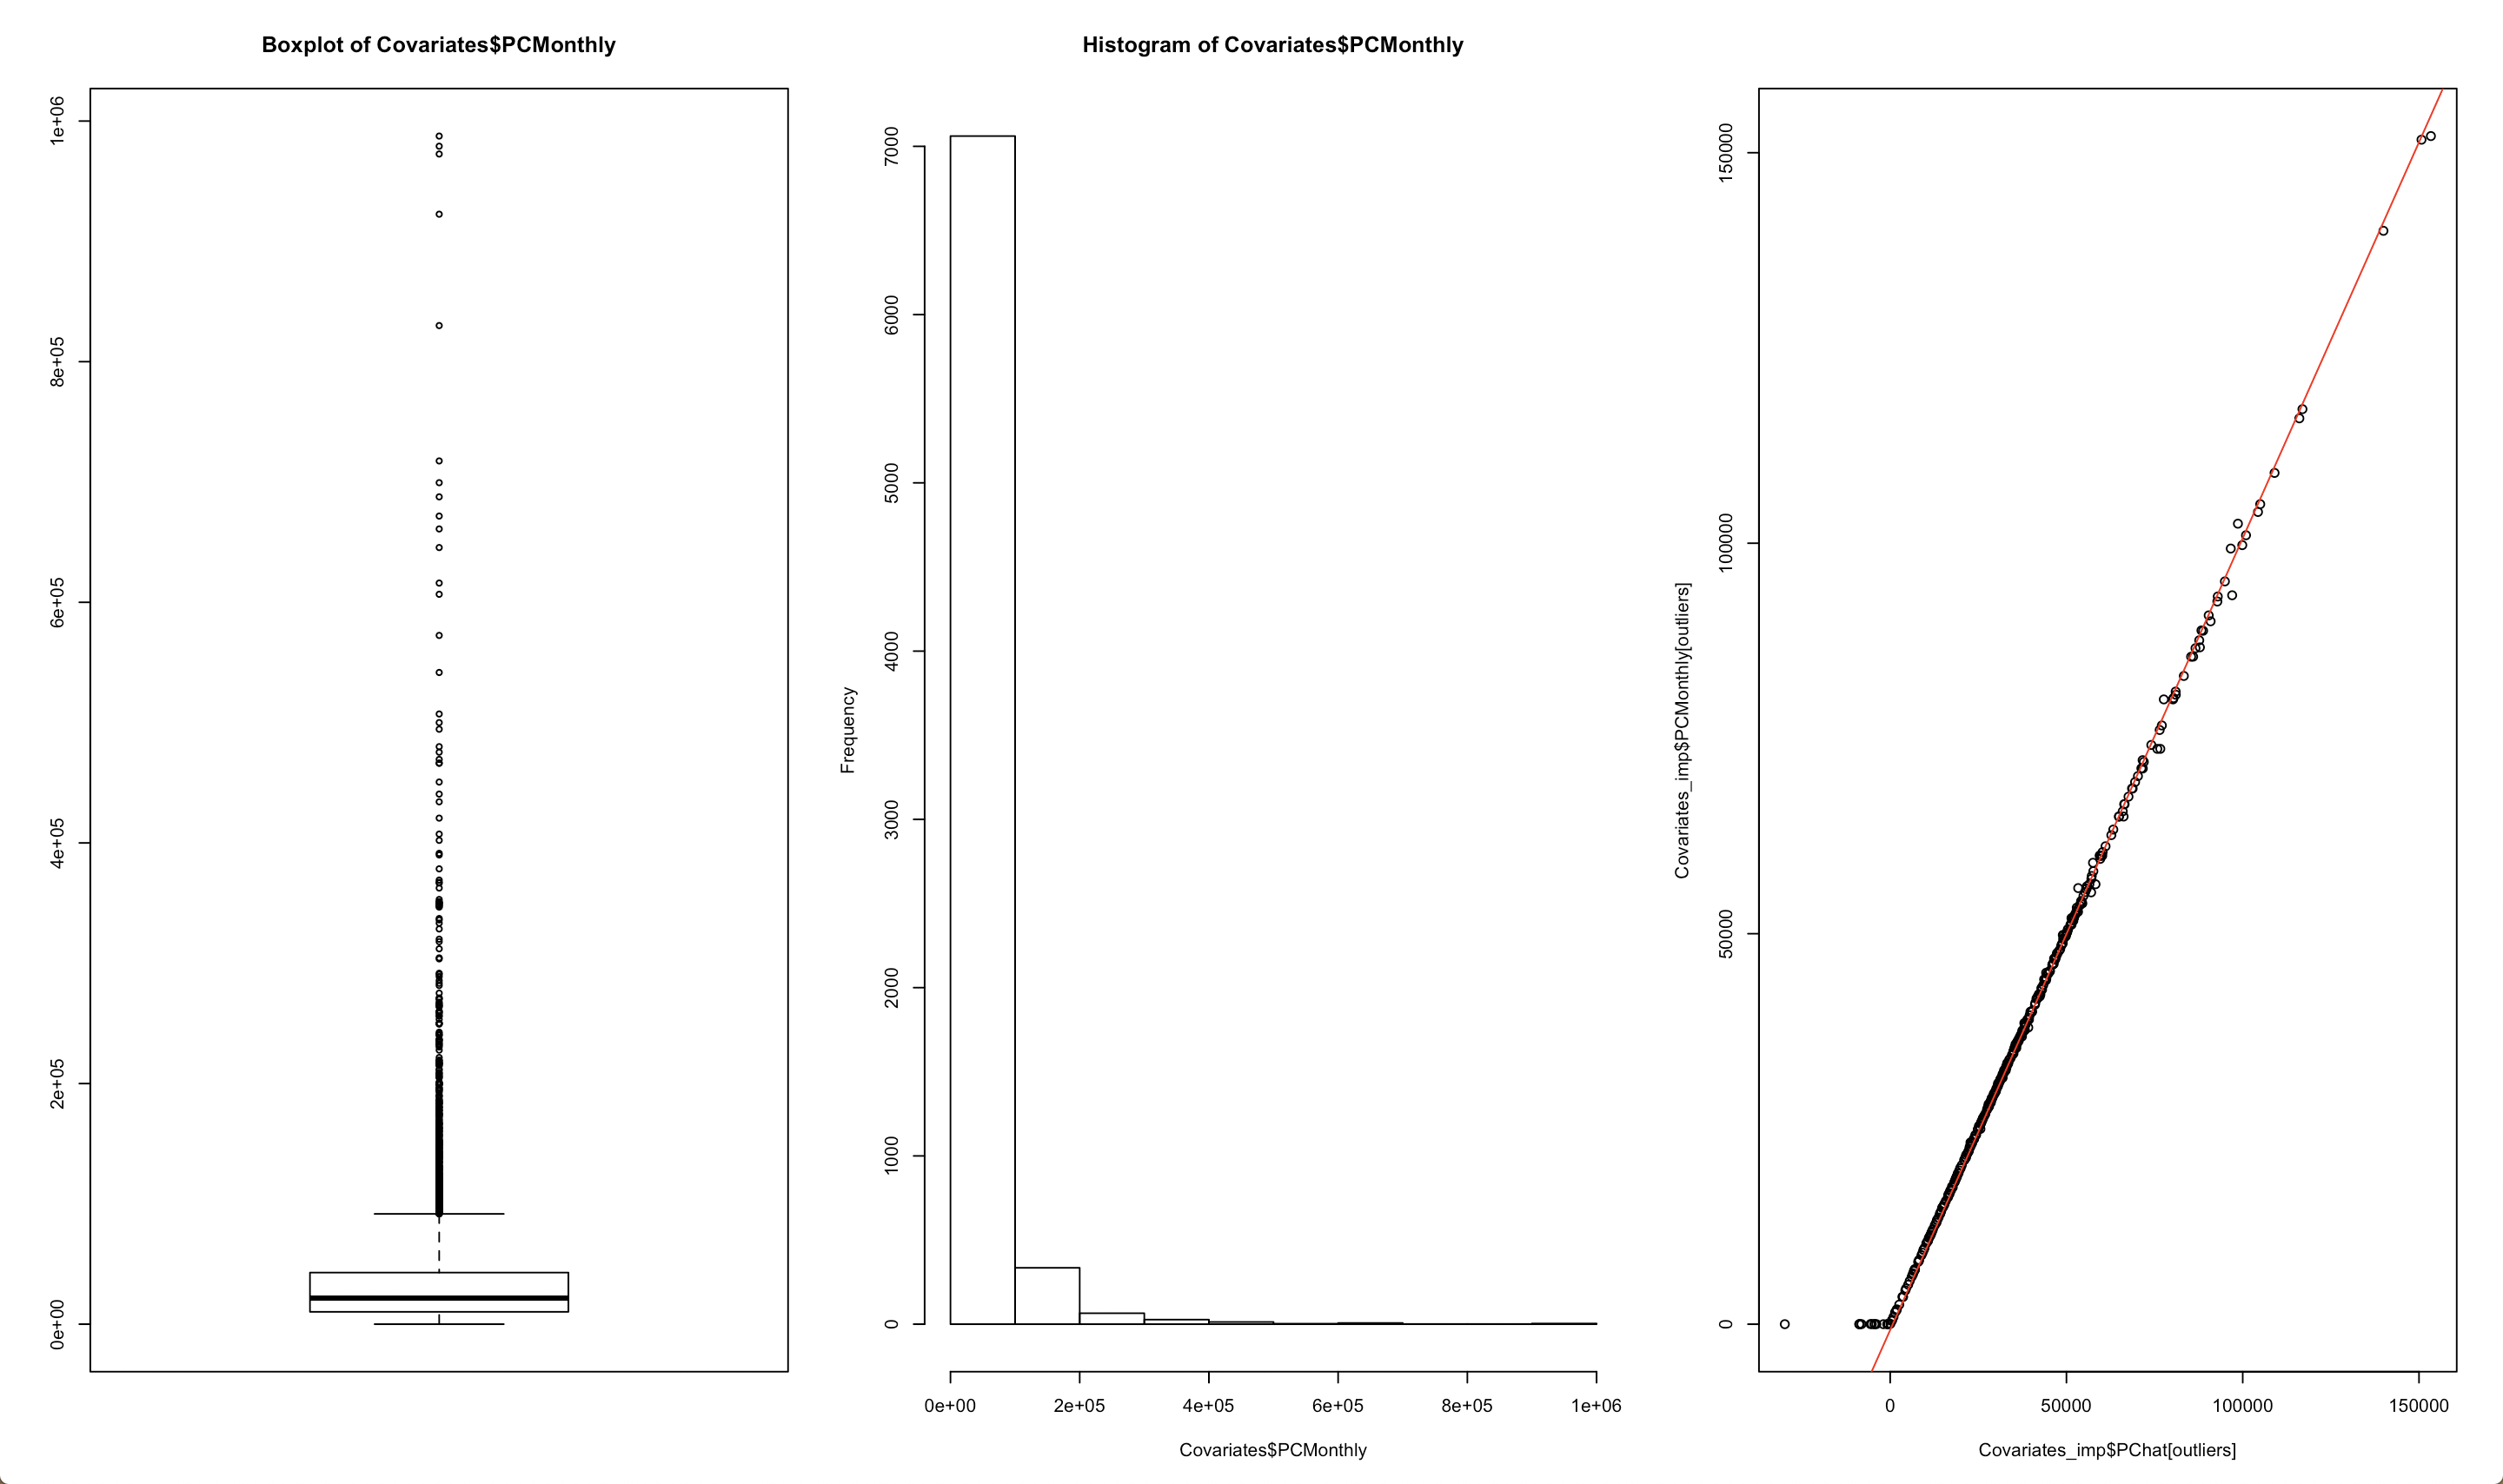
\includegraphics[width=0.5\linewidth]{Pics/10} \caption{Distribución de los ingresos (izquierda y centro) y Relación entre los valores predichos e imputados para los hogares con datos de ingresos faltantes (derecha).}\label{fig:fig10}
\end{figure}

Por último, nótese que si la base de datos contiene hogares que reportaron un ingreso nulo en todo el año, es posible que esos valores se consideren como faltantes porque se asume que la probabilidad de que un hogar no genere ningún tipo de ingreso durante todo un año es bastante baja. Además, los hogares con ingresos superiores a un límite también pueden ser considerados como valores atípicos y luego ser imputados.

\hypertarget{imputaciuxf3n-del-filtro}{%
\subsection{Imputación del filtro}\label{imputaciuxf3n-del-filtro}}

El siguiente paso, luego de haber logrado imputar con éxito las covariables determinantes del gasto, es precisamente utilizarlas para lograr imputar el gasto en bienes o servicios. Por lo general, las encuestas de ingresos y gastos preguntan si el hogar consumió o adquirió cierto bien o servicio específico. En caso de responder afirmativamente, se pregunta por la cantidad de dinero gastado en el bien o servicio y por la cantidad de artículos adquiridos en el periodo de referencia; en caso de responder negativamente, se procede a preguntar por el siguiente bien o servicio. Por supuesto, diferentes artículos tiene diferentes tasas de respuesta en sus filtros. De aquí en adelante, el valor a ser imputado en esta etapa es dicotómico: sí o no. Si el valor imputado hubiera sido no, eso significaría que el hogar no debería tener ningún gasto asociado a ese registro. Debido a la naturaleza del filtro, un modelo de regresión logística es conveniente para modelar la ausencia de respuesta en el filtro. De esta manera, la probabilidad de consumo (o compra) a un artículo \(i\) en particular es \(p_k = Pr(Filtro_i = 1)\) y puede ser estimada por medio del siguiente modelo de regresión logística:

\[
\tilde{p}_k = logit^{-1}(\mathbf{x}_k \hat{\boldsymbol{\beta}}_i) =
\frac{exp(\mathbf{x}_k \hat{\boldsymbol{\beta}}_i)}{1+exp(\mathbf{x}_k \hat{\boldsymbol{\beta}}_i)}
\]

Las covariables incluidas en la matriz \(\mathbf{x}\) podrían ser las mismas utilizados para la imputación de los ingresos y, por supuesto, los ingresos en sí. Es decir, las covariables incluidas serían la composición del hogar, el estado ocupación y fuerza de trabajo de los miembros del hogar, la calidad de la vivienda, la ubicación del hogar y los ingresos del hogar. Asumiendo que los similares valores de \(\tilde p\) producirán valores de filtro similares, podemos ``pedir prestado'' un valor de filtro para imputar el que falta de un vecino con un valor similar de \(\tilde p\). Por lo tanto, el valor imputado del filtro para la unidad \(k\) es dado por \(Filtro_k = Filtro_{l(k)}\); donde \(l(k)\) es el elemento donante, determinado por la minimización de la distancia \(D_{lk} = |\tilde p_k - p_l|\). Se enfatiza en que el donante \(l\) del elemento \(k\) es el elemento en el conjunto \(r_i\) con el valor más pequeño de la distancia \(D_{lk}\).

Por regla general, todo los donantes deben estar en la misma provincia que la unidad con el valor faltante. Por ejemplo, considere el artículo arroz, para el cual algunos hogares no proveyeron ninguna respuesta asociada al filtro de compra. Como este es un artículo de consumo masivo en nuestra región, se supondría que la mayoría de hogares respondiera que efectivamente ha comprado arroz en el periodo de referencia. De esta manera, al utilizar la regresión logística como modelo para la ausencia de respuesta del filtro del arroz, es posible encontrar que la distribución de las probabilidades estimadas de compra de arroz esté sesgada hacia el valor uno y alejada del valor cero, como lo muestra la figura \ref{fig:fig11}. Está claro que la distribución de los valores imputados también debería estar cargada hacia el uno, reflejando la realidad de la compra de un artículo esencial como el arroz.

\begin{figure}
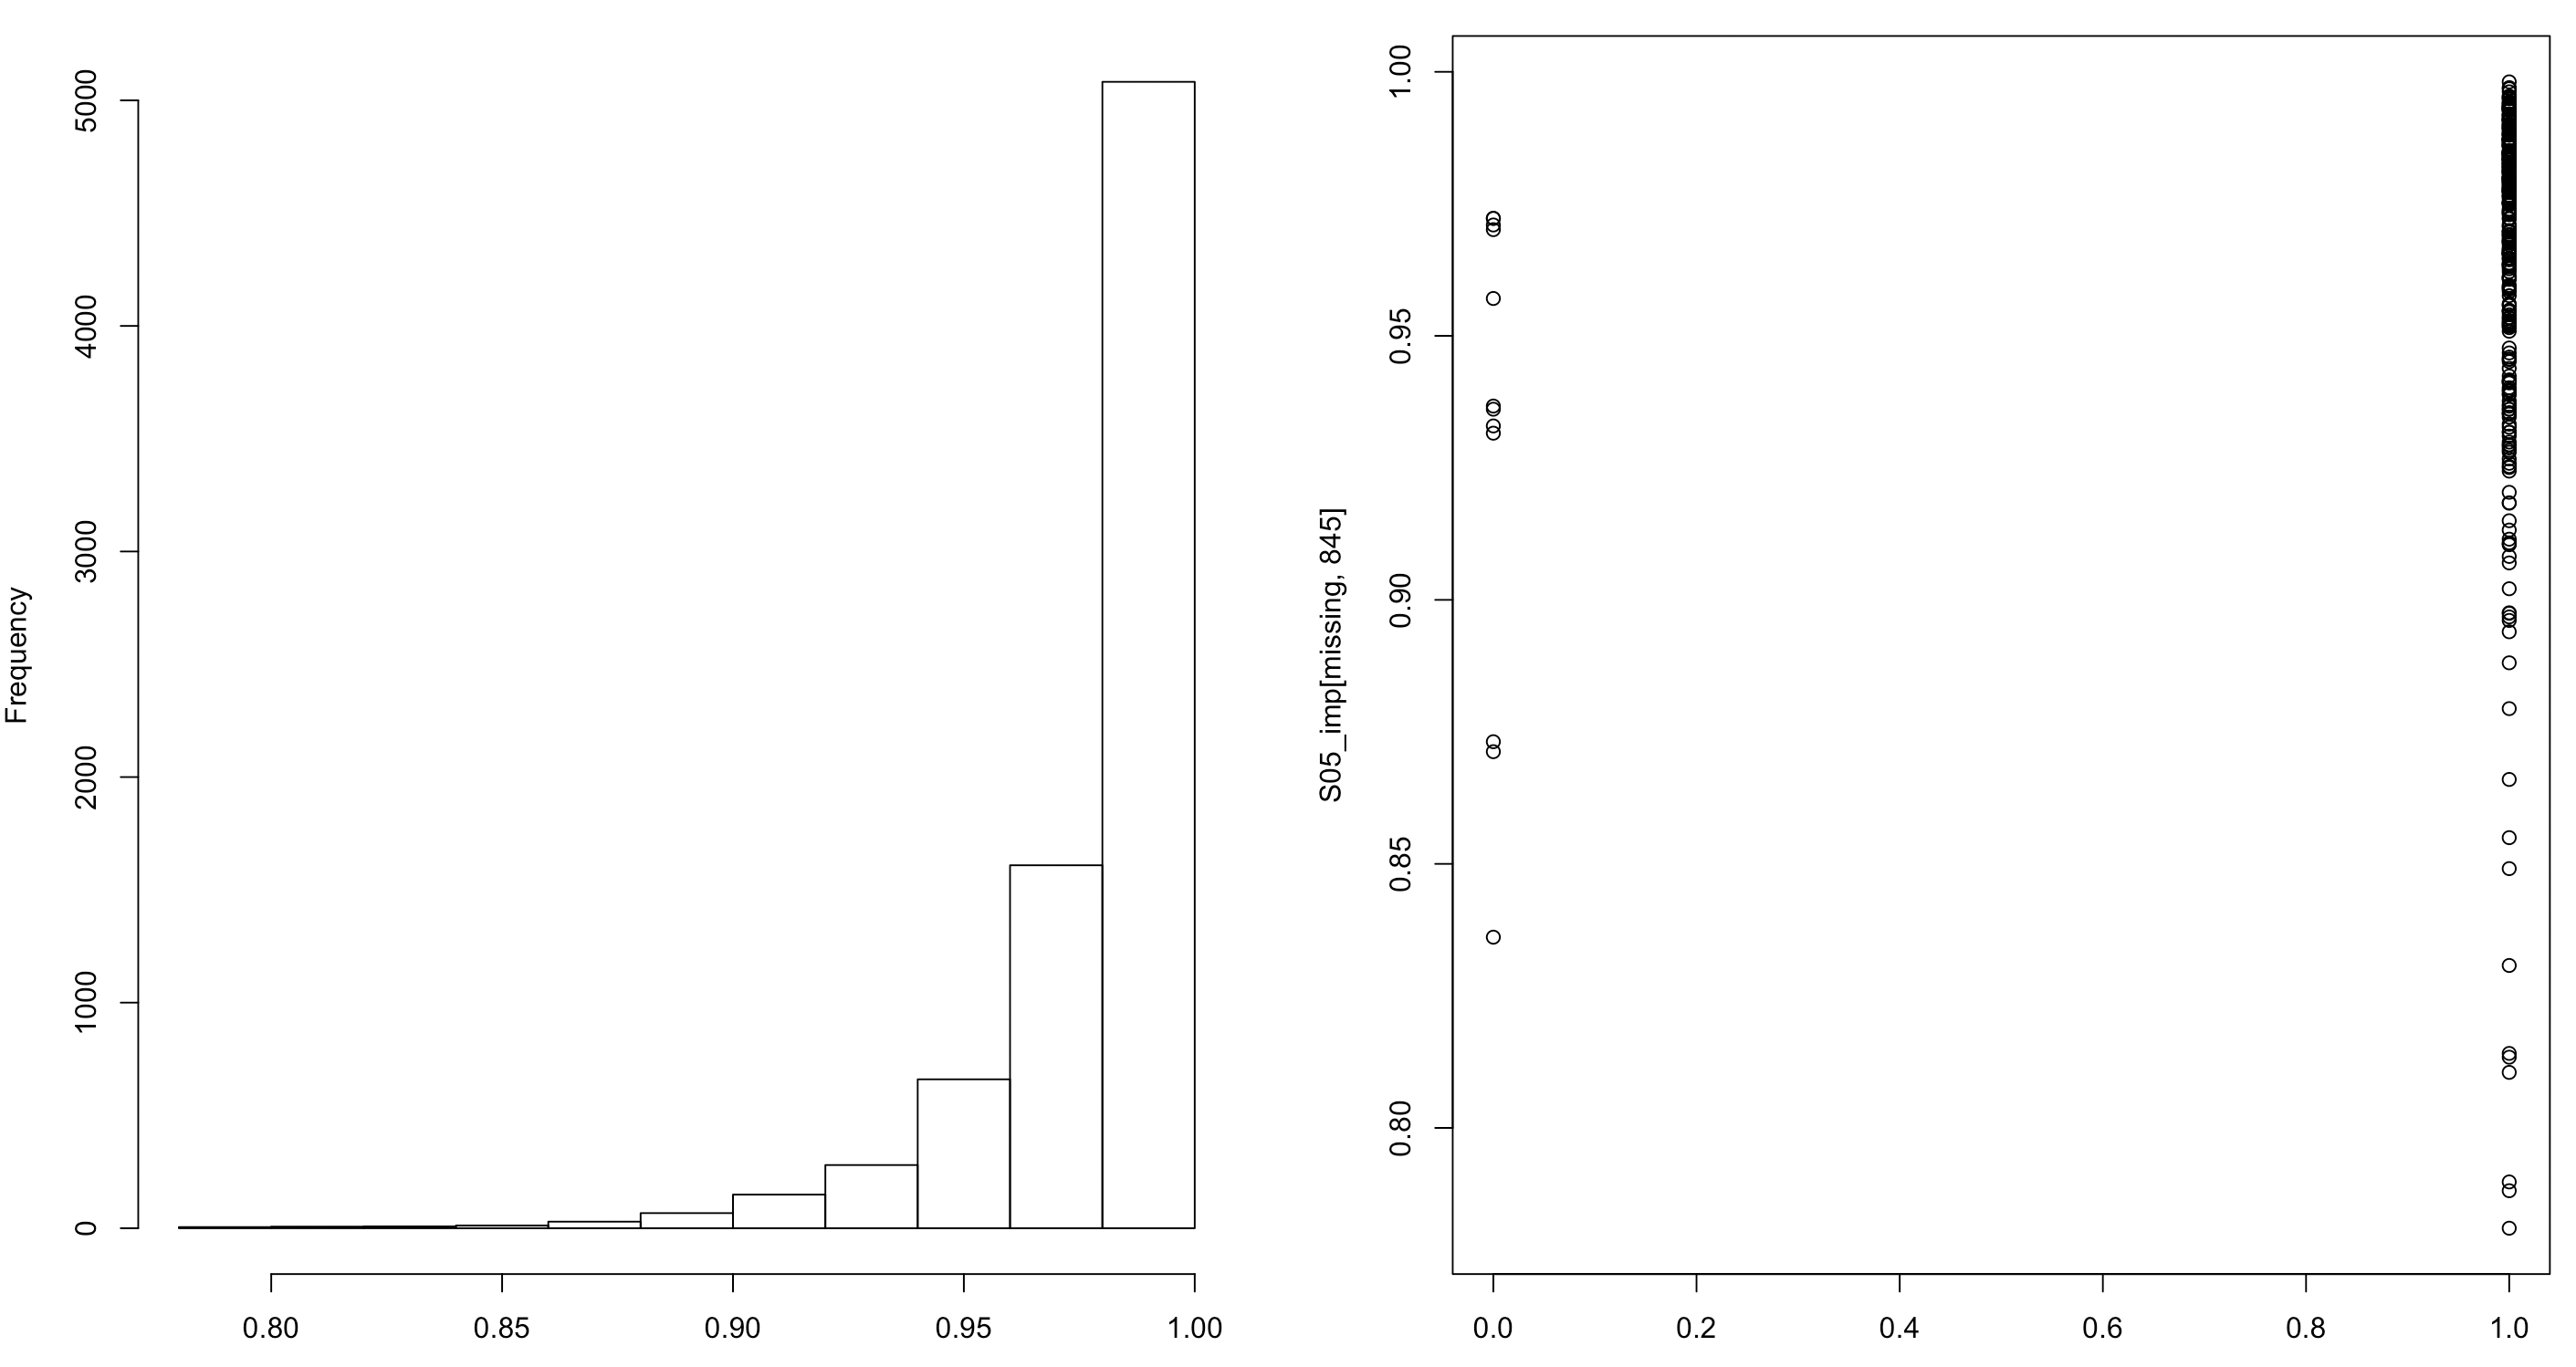
\includegraphics[width=0.5\linewidth]{Pics/11} \caption{Distribución de las probabilidades estimadas de compra de arroz (izquierda) y valores imputados para los hogares con valores faltantes en el filtro (derecha).}\label{fig:fig11}
\end{figure}

Por otro lado, el filtro para algunos artículos de bajo consumo estará más sesgado hacia el valor cero. La figura \ref{fig:fig12} muestra la distribución de las probabilidades estimadas de compra de un artículo de bajo consumo, así como los valores imputados.

\begin{figure}
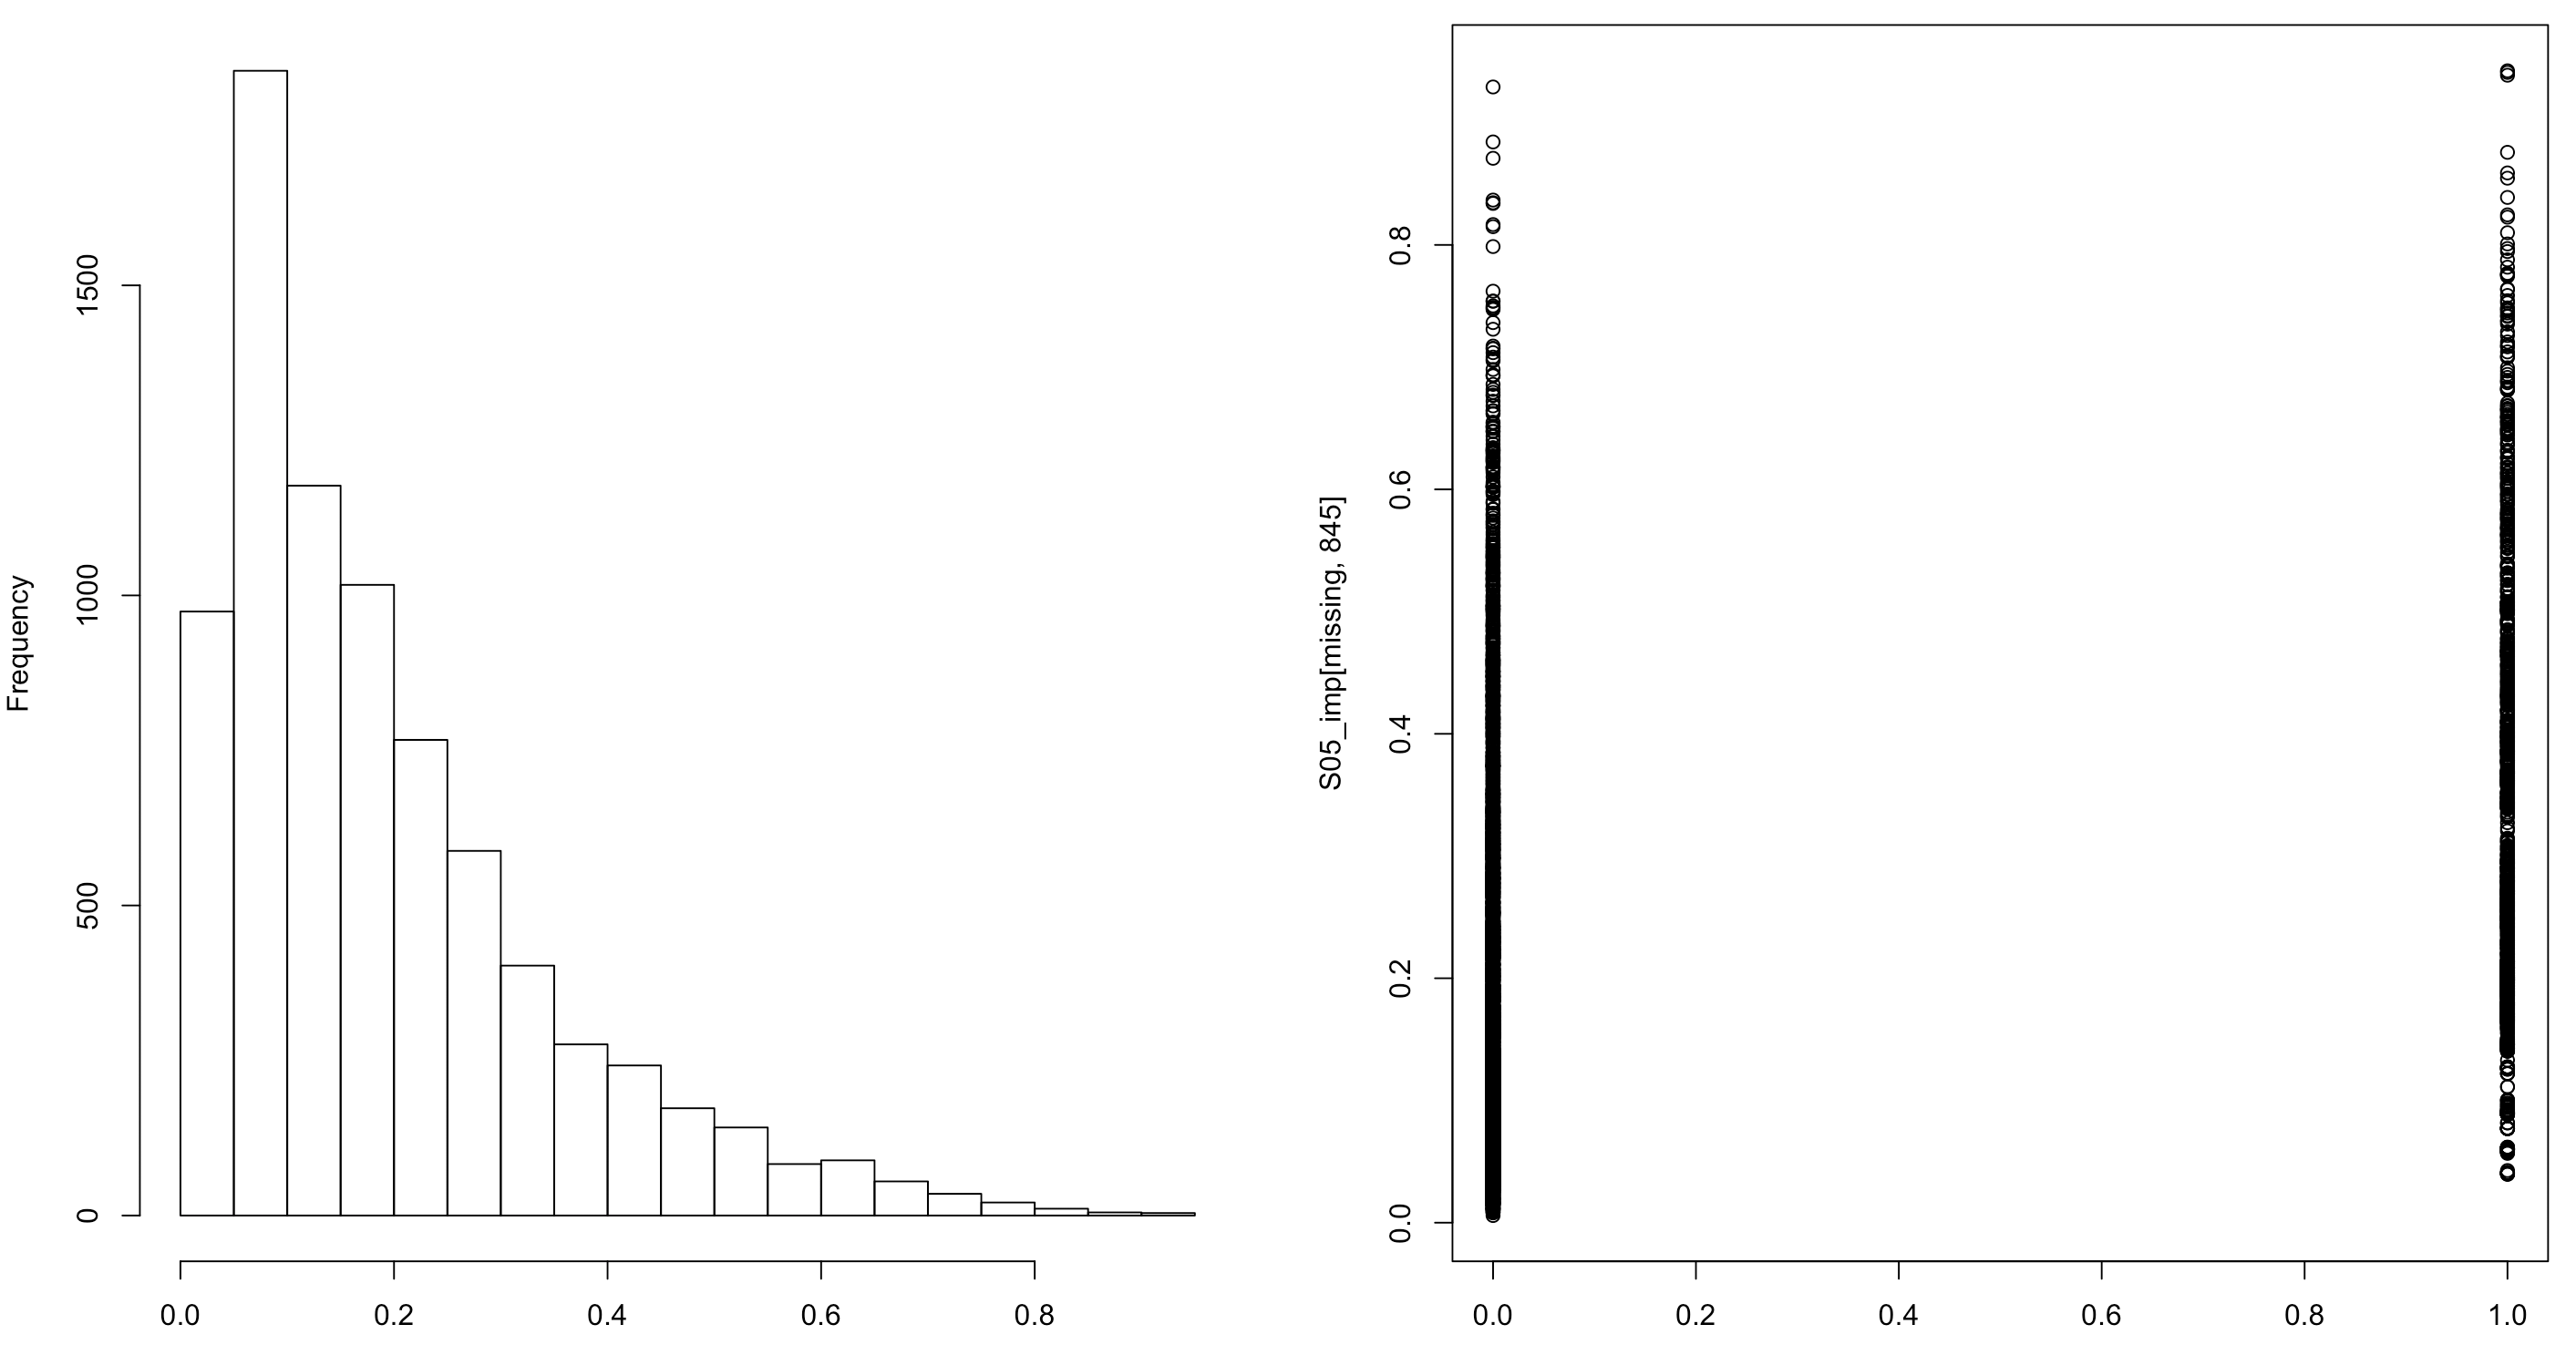
\includegraphics[width=0.5\linewidth]{Pics/12} \caption{Distribución de la probabilidad estimada de compra de un artículo de bajo consumo (izquierda) y sus valores imputados para los hogares que no respondieron el filtro (derecha).}\label{fig:fig12}
\end{figure}

\hypertarget{imputaciuxf3n-del-gasto}{%
\subsection{Imputación del gasto}\label{imputaciuxf3n-del-gasto}}

Éste es el paso final del proceso de imputación y está fuertemente influenciado por los resultados de la imputación de la pregunta de filtro. En este paso, los hogares cuyo valor imputado de filtro es cero automáticamente tendrá un cero imputado como la cantidad de dinero gastado en ese artículo. Es decir, si el resultado de la imputación en el filtro es cero, esto implica directamente que el hogar no compró (o produjo) el artículo en el periodo de referencia, y por tanto la frecuencia de compra, la cantidad que registros comprados y la cantidad de dinero gastado en ese artículo debe ser cero. Las unidades restantes deben tener un valor observado o imputado de uno en el filtro, y por lo tanto los valores faltantes del gasto deben ser imputados.

Observe que el grupo de donantes está restringido a los que tienen un valor de gasto distinto de cero en el artículo específico. Es decir, para aquellas unidades con un valor de filtro distinto de cero, un donante debe ser identificado. Para la imputación del gasto, la técnica del vecino más cercano con el método de regresión puede considerarse en el mismo sentido que fue implementado en la imputación de los ingresos. Por lo tanto, se considera un modelo lineal en donde las covariables incluidas en la matriz \(\mathbf{x}\) son la composición del hogar, el estado de ocupación y fuerza de trabajo, la calidad de la vivienda, la ubicación del hogar y los ingresos.

Volviendo a los ejemplos anteriores, la figura \ref{fig:fig13} muestra la distribución de los gastos imputados en consumo de salmón. Se nota que la cantidad de dinero gastado en este artículo es baja y que la relación entre los valores pronosticados del modelo y los valores imputados es fuertemente lineal.

\begin{figure}
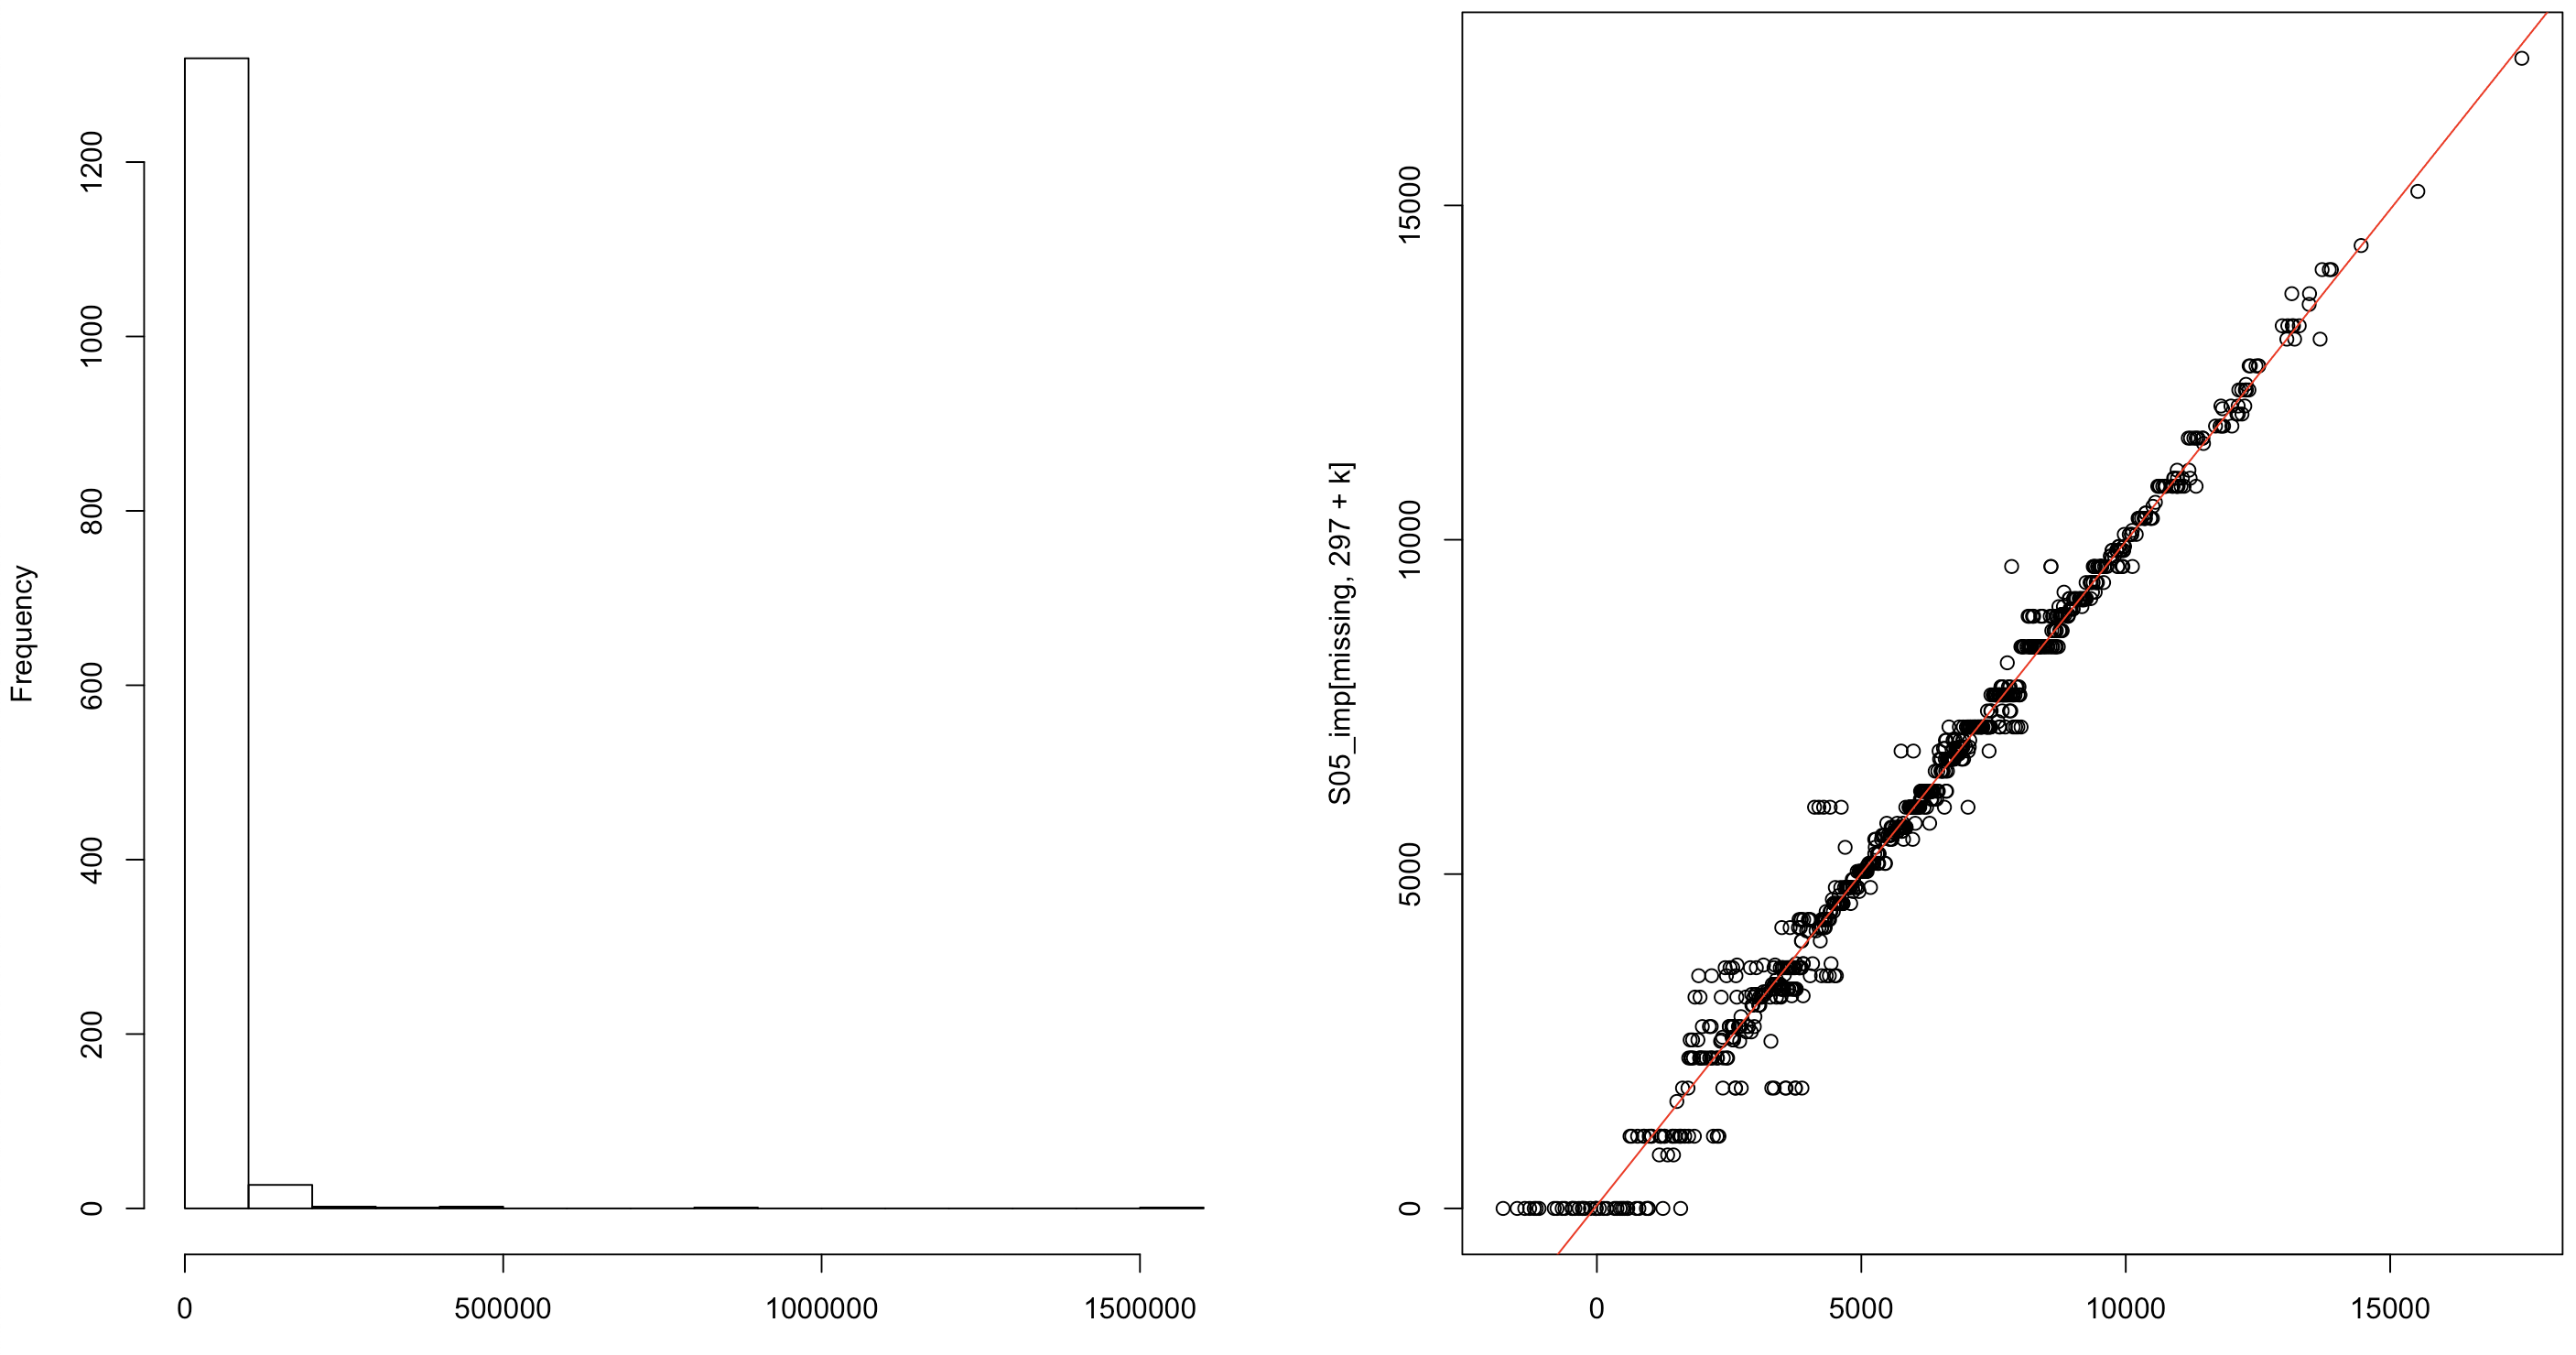
\includegraphics[width=0.5\linewidth]{Pics/13} \caption{Distribución de los gastos imputados sobre el salmón (izquierda) y relación entre los valores predichos e imputados para los hogares con valores faltantes en el gasto (derecha).}\label{fig:fig13}
\end{figure}

\hypertarget{consideraciones-sobre-la-imputaciuxf3n-muxfaltiple}{%
\section{Consideraciones sobre la imputación múltiple}\label{consideraciones-sobre-la-imputaciuxf3n-muxfaltiple}}

Antes de escoger un método particular, es pertinente observar qué efectos conlleva esta escogencia en las propiedades estadísticas de los estimadores en las encuestas de hogares. En cuanto a la imputación múltiple, las propiedades estadísticas de los estimadores deben ser modificadas acordemente. Subestimar la variación de las estimaciones puede ser un error muy grave, puesto que afecta la cobertura nominal de los intervalos de confianza y a su vez influye en las pruebas de hipótesis y en el cálculo de los valores \(p\).

Por ejemplo, suponga que existe una muestra aleatoria \(s\) compuesta por un conjunto de \(n\) datos que relacionan dos variables \(X\), \(Y\), a través del siguiente modelo de regresión simple:

\[
y_k = \beta x_k + \varepsilon_k
\]

En donde los errores tienen distribución normal con \(E(\varepsilon_k) = 0\) y \(Var(\varepsilon_k) = \sigma ^2\) para todo \(k\in s\). Bajo esta perspectiva, suponga que la variable dependiente de interés sólo pudo ser observada para un conjunto de individuos de tamaño \(n_1\), mientras que para los \(n_0\) individuos restantes (es decir, \(n_1 + n_0 = n\)), no existen datos para la variable de interés; además se asume que sí fue posible observar los valores de la covariable \(X\) para todos los individuos en la muestra.

El valor agregado de la imputación múltiple \citep{Rubin_1987} realmente está en la estimación de los errores estándar. No tener en cuenta la naturaleza estocástica de los valores imputados arroja estimaciones de la varianza mucho menores. La idea consiste en generar \(M > 1\) conjuntos de valores para los registros faltantes. Al final, el valor \emph{imputado} corresponderá al promedio de esos \(M\) valores. Por tanto el modelo final de imputación (para los valores faltantes) toma la siguiente forma:

\[\dot{y}_i = \dot{\beta} x_{i_{(missing)}}+ \dot{\varepsilon_i}\]

Para este caso, se consideran dos maneras de realizar la imputación; la primera basada en la esperanza del modelo (sin imputación múltiple) y la segunda basada en la adición del término de error del modelo (imputación múltiple):

\begin{itemize}
\tightlist
\item
  \textbf{Ingenua}: en este escenario, el valor imputado para el registro faltante toma la siguiente forma:
  \[
  \dot{y}_i = \hat\beta x_{i_{(missing)}}
  \]
  Esta clase de imputación carece de aleatoriedad y por tanto, la varianza de \(\beta\) será subestimada.
\item
  \textbf{Múltiple}: en este caso, se tiene en cuenta el término de error en la generación de los valores imputados, tales que
  \[
  \dot{y}_i = \dot{\beta} x_{i_{(missing)}}+ \dot{\varepsilon_i}
  \]
\end{itemize}

Es posible realizar la imputación múltiple de forma frecuentista o bayesiana. Por ejemplo, es posible seleccionar \(M\) muestras \emph{bootstrap}, y para cada una se estiman los parámetros \(\beta\) y \(\sigma\) para generar \(\dot{y}_i\). Al final se promedian los \(M\) valores y se imputa el valor faltante. Por otro lado, teniendo en cuenta el acercamiento bayesiano, se definen las distribuciones posteriores de \(\beta\) y \(\sigma\) para generar \(M\) valores de estos parámetros y por tanto \(M\) valores de \(\dot{y}_i\). De igual manera, al final se promedian los \(M\) valores y se imputa el valor faltante.

Por ejemplo, si el interés es la estimación de un parámetro \(\beta\), entonces la esperanza estimada al utilizar la metodología de imputación múltiple está dada por:

\[
E(\hat{\beta} | Y_{obs}) = E(E(\hat{\beta} | Y_{obs}, Y_{mis}) | Y_{obs})
\]

Esta expresión es estimada por el promedio de las \(M\) estimaciones puntuales de \(\hat{\beta}\) sobre las \(M\) imputaciones, dado por:

\[
\bar{\hat{\beta}} = \frac{1}{M} \sum_{m = 1} ^ M \hat{\beta}_m
\]

Entre tanto, la varianza estimada al utilizar la metodología de imputación múltiple está dada por la siguiente expresión:

\[
V(\hat{\beta} | Y_{obs}) = E(V(\hat{\beta} | Y_{obs}, Y_{mis}) | Y_{obs}) +
V(E(\hat{\beta} | Y_{obs}, Y_{mis}) | Y_{obs}) 
\]

La primera parte de la anterior expresión se estima como el promedio de las varianzas muestrales de \(\hat{\beta}\) sobre las \(M\) imputaciones, dado por:

\[
\bar{U} = \frac{1}{M} \sum_{m = 1} ^ M Var(\hat{\beta})
\]

El segundo término se estima como la varianza muestral de las \(M\) estimaciones puntuales de \(\hat{\beta}\) sobre las \(M\) imputaciones, dada por:
\[
B = \frac{1}{M-1} \sum_{m = 1} ^ M (\hat{\beta}_m - \bar{\hat{\beta}})^2
\]

Además, es necesario tener en cuenta un factor de corrección (puesto que \(M\) es finito). Por tanto, la estimación del segundo término viene dada por la siguiente expresión:

\[
\left(1 + \frac{1}{M}\right) B
\]

Por tanto, la varianza estimada es igual a:

\[
\hat{V}(\hat{\beta} | Y_{obs}) = \bar{U} + \left(1 + \frac{1}{M}\right) B
\]

Por ejemplo, si se quiere realizar mediciones de pobreza utilizando la imputación múltiple es necesario primero establecer un modelo sobre los ingresos \(y_k\) y luego generar \(Q\) posibles valores \(y_k^q \ (q=1, \ldots, Q)\) para cada individuo que no respondió. Luego, utilizando los \(Q\) conjuntos de datos completos, es necesario estimar la siguientes cantidades

\[
\hat{F}_{\alpha}^{q}=\frac{1}{N}\sum_{k\in s} w_k 
\left(\frac{l-y_k}{l}\right)^{\alpha}I(y_k<l) \ \ \ \ \ \ \ \ \ 
q= 1,\ldots, Q.
\]

El estimador final basado en la técnica de imputación múltiple será el promedio simple de las anteriores estimaciones, dado por

\[
\tilde{F}_{\alpha}=\frac{1}{Q}\sum_{q=1}^Q \hat{F}_{\alpha}^{q}
\]

La varianza de esta metodología se puede dividir en dos componentes, el primero correspondiente a la variación dentro de cada conjunto de datos creado, y el segundo correspondiente a la variación entre cada estimación resultante. Por lo tanto, la varianza asociada a \(\tilde{F}_{\alpha}\) es

\[
\hat{V}(\tilde{F}_{\alpha})
= \frac{1}{Q}\sum_{q=1}^Q \hat{V}(\hat{F}_{\alpha}^{q})
+ \left(1+\frac{1}{Q}\right)\frac{1}{Q-1}\sum_{q=1}^Q (\hat{F}_{\alpha}^{q}-\tilde{F}_{\alpha})^2
\]

Una vez que se tienen los conjuntos de datos completos, es posible estimar \(\hat{V}(\hat{F}_{\alpha}^{q})\) utilizando las técnicas del último conglomerado en conjunción con el Jackkinfe. La característica principal del proceso imputación es utilizar la información auxiliar para aproximar con precisión los valores faltantes. De esta forma, las estimaciones poblacionales de los parámetros de interés tendrán sesgo nulo o despreciable y la confiabilidad de la estrategia de muestreo se mantendrá como se planeó en una primera instancia. L siguiente simulación ejemplifica las ventajas de la imputación múltiple.

\hypertarget{simulaciuxf3n-empuxedrica}{%
\subsection{Simulación empírica}\label{simulaciuxf3n-empuxedrica}}

Para ejemplificar los anteriores escenarios, en esta sección se muestran los resultados empíricos de una simulación que asumió un conjunto de \(n = 100\) datos con una pendiente \(\beta = 100\) y con una dispersión de \(\sigma = 2\). A su vez, el conjunto de datos tendrá \(n_0 = 40\) valores faltantes en la variable respuesta. A continuación se muestran las primeras diez filas de esta base de datos simulados. Nótese que las dos primeras columnas corresponden a los valores verdaderos de la covariable y la variable de interés, respectivamente. La tercera columna identifica cuáles de estos valores son faltantes y la cuarta columna representaría la información disponible en la base de datos de la muestra \(s\).

\begin{longtable}[]{@{}cccc@{}}
\caption{Ejemplo de un conjunto de datos con valores faltantes.}\tabularnewline
\toprule()
x & y & faltantes & y (no imputado) \\
\midrule()
\endfirsthead
\toprule()
x & y & faltantes & y (no imputado) \\
\midrule()
\endhead
11 & 991 & Si & NA \\
12 & 1282 & Si & NA \\
12 & 1164 & No & 1164 \\
12 & 1217 & No & 1217 \\
13 & 1325 & No & 1325 \\
11 & 1086 & No & 1086 \\
12 & 1210 & Si & NA \\
13 & 1272 & Si & NA \\
15 & 1459 & Si & NA \\
11 & 1182 & No & 1182 \\
\bottomrule()
\end{longtable}

Con el 40\% de valores faltantes, es necesario realizar una imputación para obtener registros completos en la base de datos. Para este ejemplo, la figura \ref{fig:figim1} relaciona las variables con (izquierda) y sin (derecha) valores faltantes se presentan a continuación.

\begin{figure}
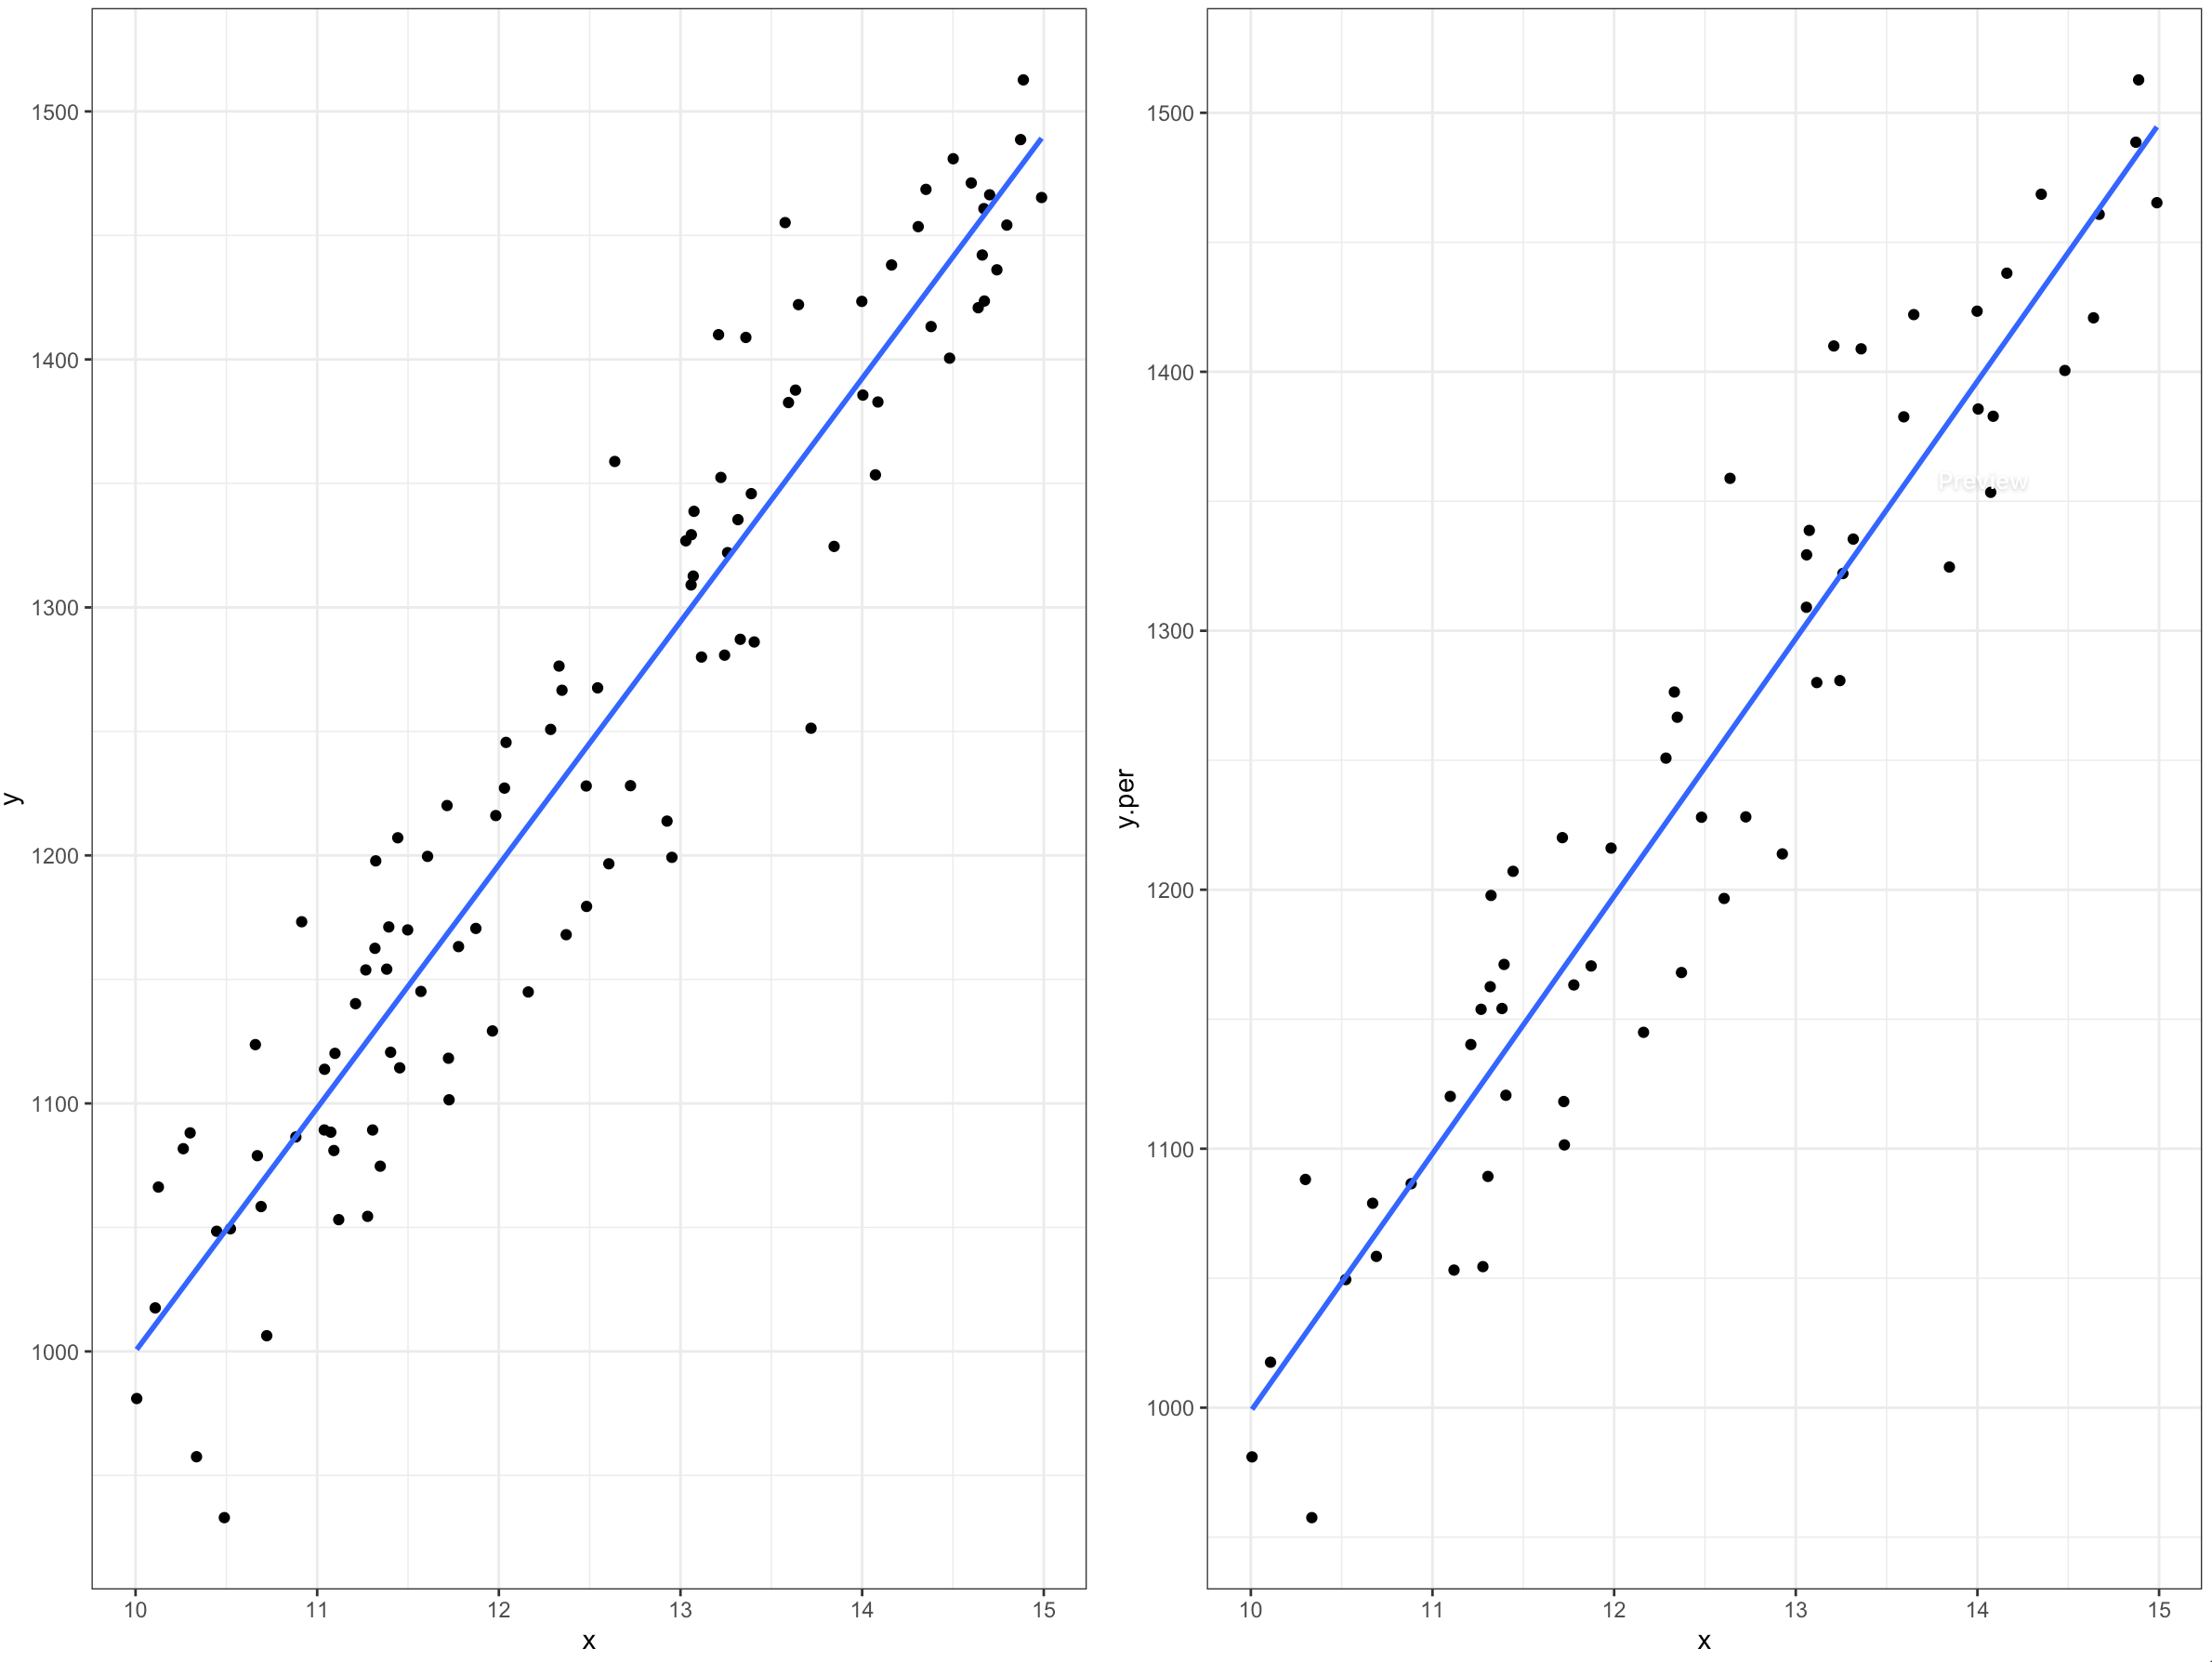
\includegraphics[width=0.5\linewidth]{Pics/im1} \caption{Relación de la variable de interés para los datos completos (izquierda) y con ausencia de valores (derecha).}\label{fig:figim1}
\end{figure}

Al aplicar una imputación ingenua, por ejemplo basada en un modelo de regresión simple, se obtendría un conjunto de datos completo, ejemplificado (solo las primeras diez filas de la base) en la siguiente tabla:

\begin{longtable}[]{@{}cccc@{}}
\caption{Ejemplo de un conjunto de datos con valores imputados ingenuamente.}\tabularnewline
\toprule()
x & y (original) & faltantes & y (imputado) \\
\midrule()
\endfirsthead
\toprule()
x & y (original) & faltantes & y (imputado) \\
\midrule()
\endhead
11 & 991 & Si & 1047 \\
12 & 1282 & Si & 1221 \\
12 & 1164 & No & 1164 \\
12 & 1217 & No & 1217 \\
13 & 1325 & No & 1325 \\
11 & 1086 & No & 1086 \\
12 & 1210 & Si & 1221 \\
13 & 1272 & Si & 1290 \\
15 & 1459 & Si & 1485 \\
11 & 1182 & No & 1182 \\
\bottomrule()
\end{longtable}

En general, usar un enfoque simple no afecta la estimación puntual del parámetro de interés, sino la estimación del error estándar, puesto que la variación natural de los datos se subestima dramáticamente. Por ejemplo, la figura \ref{fig:figim2} muestra que con la imputación simple, \emph{todos} los valores faltantes imputados están sobre la línea de regresión.

\begin{figure}
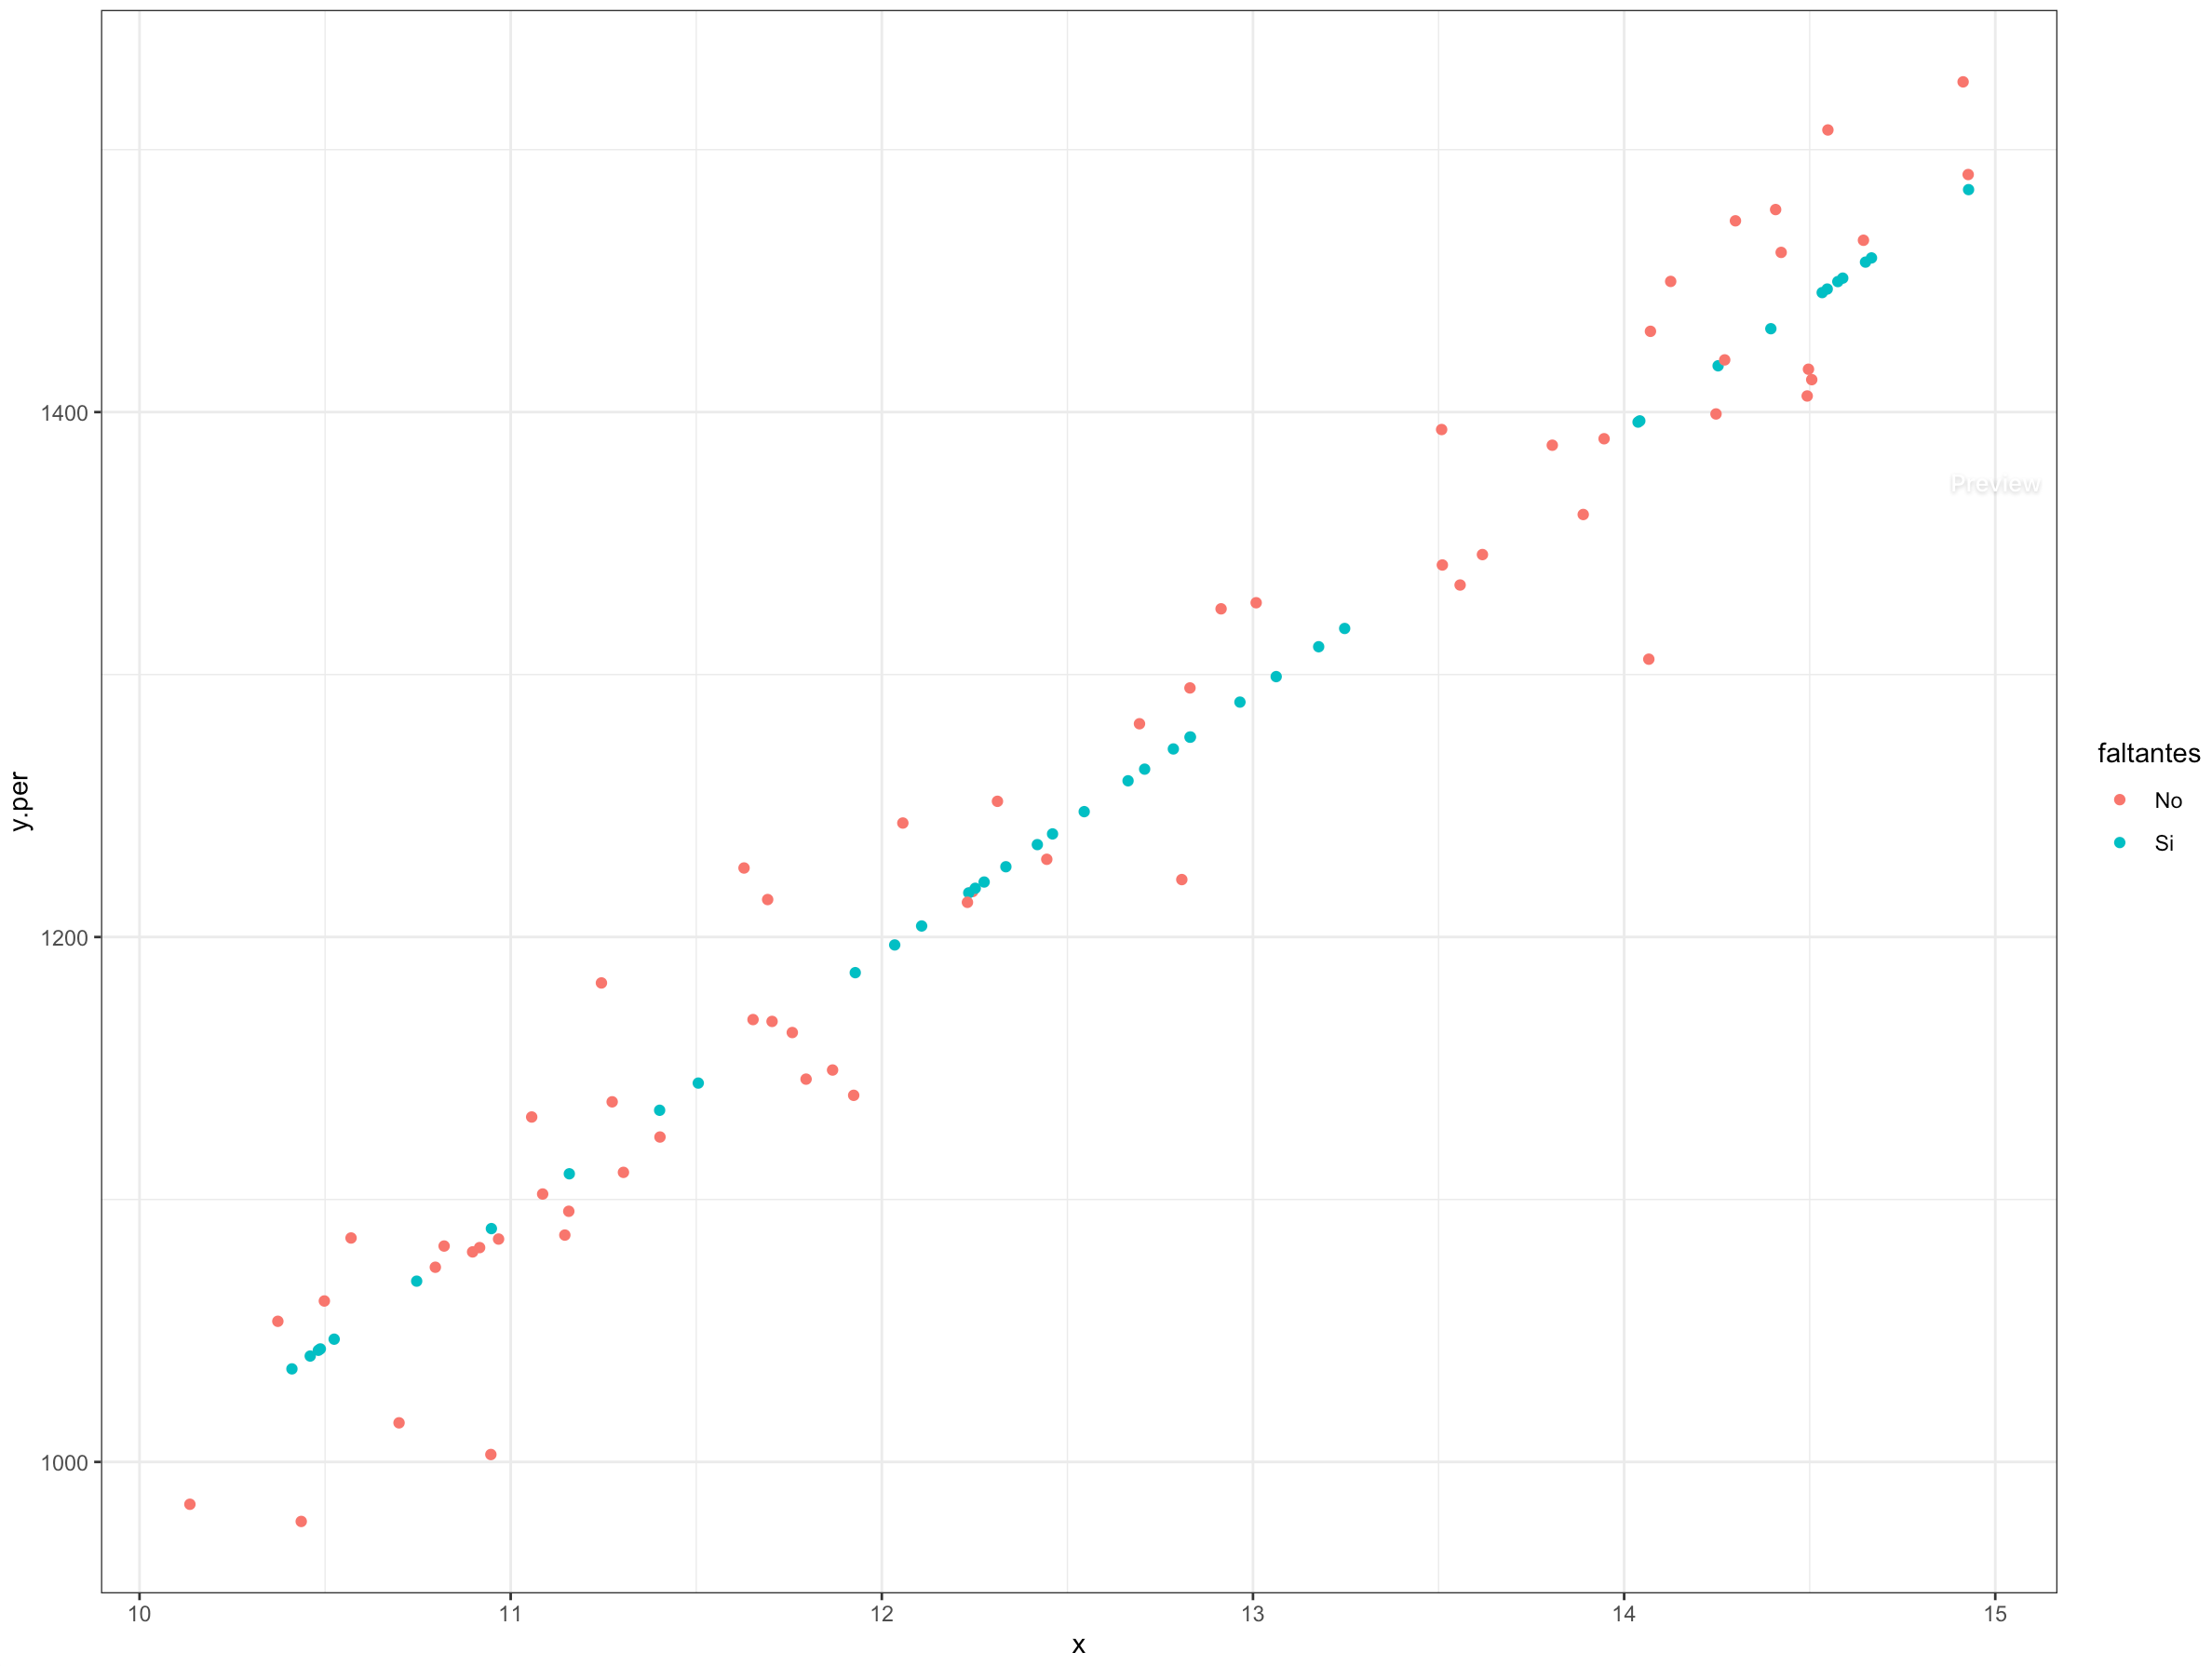
\includegraphics[width=0.5\linewidth]{Pics/im2} \caption{Relación de la variable de interés con la covariable auxiliar para el enfoque de imputación ingenua.}\label{fig:figim2}
\end{figure}

Si se considera la imputación múltiple con el enfoque \emph{bootstrap}, también se obtedrá un conjunto de datos aumentado por cada una de las \(M\) realizaciones que se ejecuten. Por ejemplo, a continuación se ilustra el conjunto de datos obtenido con \(M=3\) realizaciones. Nótese que los valores de la variable de interés cambian en cada realización; estas realizaciones se conocen en la literatura como \emph{valores plausibles}.

\begin{longtable}[]{@{}
  >{\centering\arraybackslash}p{(\columnwidth - 10\tabcolsep) * \real{0.0667}}
  >{\centering\arraybackslash}p{(\columnwidth - 10\tabcolsep) * \real{0.1867}}
  >{\centering\arraybackslash}p{(\columnwidth - 10\tabcolsep) * \real{0.1467}}
  >{\centering\arraybackslash}p{(\columnwidth - 10\tabcolsep) * \real{0.2000}}
  >{\centering\arraybackslash}p{(\columnwidth - 10\tabcolsep) * \real{0.2000}}
  >{\centering\arraybackslash}p{(\columnwidth - 10\tabcolsep) * \real{0.2000}}@{}}
\caption{Ejemplo de un conjunto de datos con múltiples (3) valores imputados.}\tabularnewline
\toprule()
\begin{minipage}[b]{\linewidth}\centering
x
\end{minipage} & \begin{minipage}[b]{\linewidth}\centering
y (original)
\end{minipage} & \begin{minipage}[b]{\linewidth}\centering
faltantes
\end{minipage} & \begin{minipage}[b]{\linewidth}\centering
y1 (imputado)
\end{minipage} & \begin{minipage}[b]{\linewidth}\centering
y2 (imputado)
\end{minipage} & \begin{minipage}[b]{\linewidth}\centering
y3 (imputado)
\end{minipage} \\
\midrule()
\endfirsthead
\toprule()
\begin{minipage}[b]{\linewidth}\centering
x
\end{minipage} & \begin{minipage}[b]{\linewidth}\centering
y (original)
\end{minipage} & \begin{minipage}[b]{\linewidth}\centering
faltantes
\end{minipage} & \begin{minipage}[b]{\linewidth}\centering
y1 (imputado)
\end{minipage} & \begin{minipage}[b]{\linewidth}\centering
y2 (imputado)
\end{minipage} & \begin{minipage}[b]{\linewidth}\centering
y3 (imputado)
\end{minipage} \\
\midrule()
\endhead
11 & 991 & Si & 1047 & 950 & 1040 \\
12 & 1282 & Si & 1221 & 1254 & 1198 \\
12 & 1164 & No & 1164 & 1164 & 1164 \\
12 & 1217 & No & 1217 & 1217 & 1217 \\
13 & 1325 & No & 1325 & 1325 & 1325 \\
11 & 1086 & No & 1086 & 1086 & 1086 \\
12 & 1210 & Si & 1252 & 1199 & 1198 \\
13 & 1272 & Si & 1304 & 1302 & 1292 \\
15 & 1459 & Si & 1485 & 1493 & 1478 \\
11 & 1182 & No & 1182 & 1182 & 1182 \\
\bottomrule()
\end{longtable}

Existe una buena dispersión en los valores imputados y la gráfica \ref{fig:figim3} muestra cómo este enfoque es mucho más realista al considerar la variación natural del fenómeno de interés en los valores imputados.

\begin{figure}
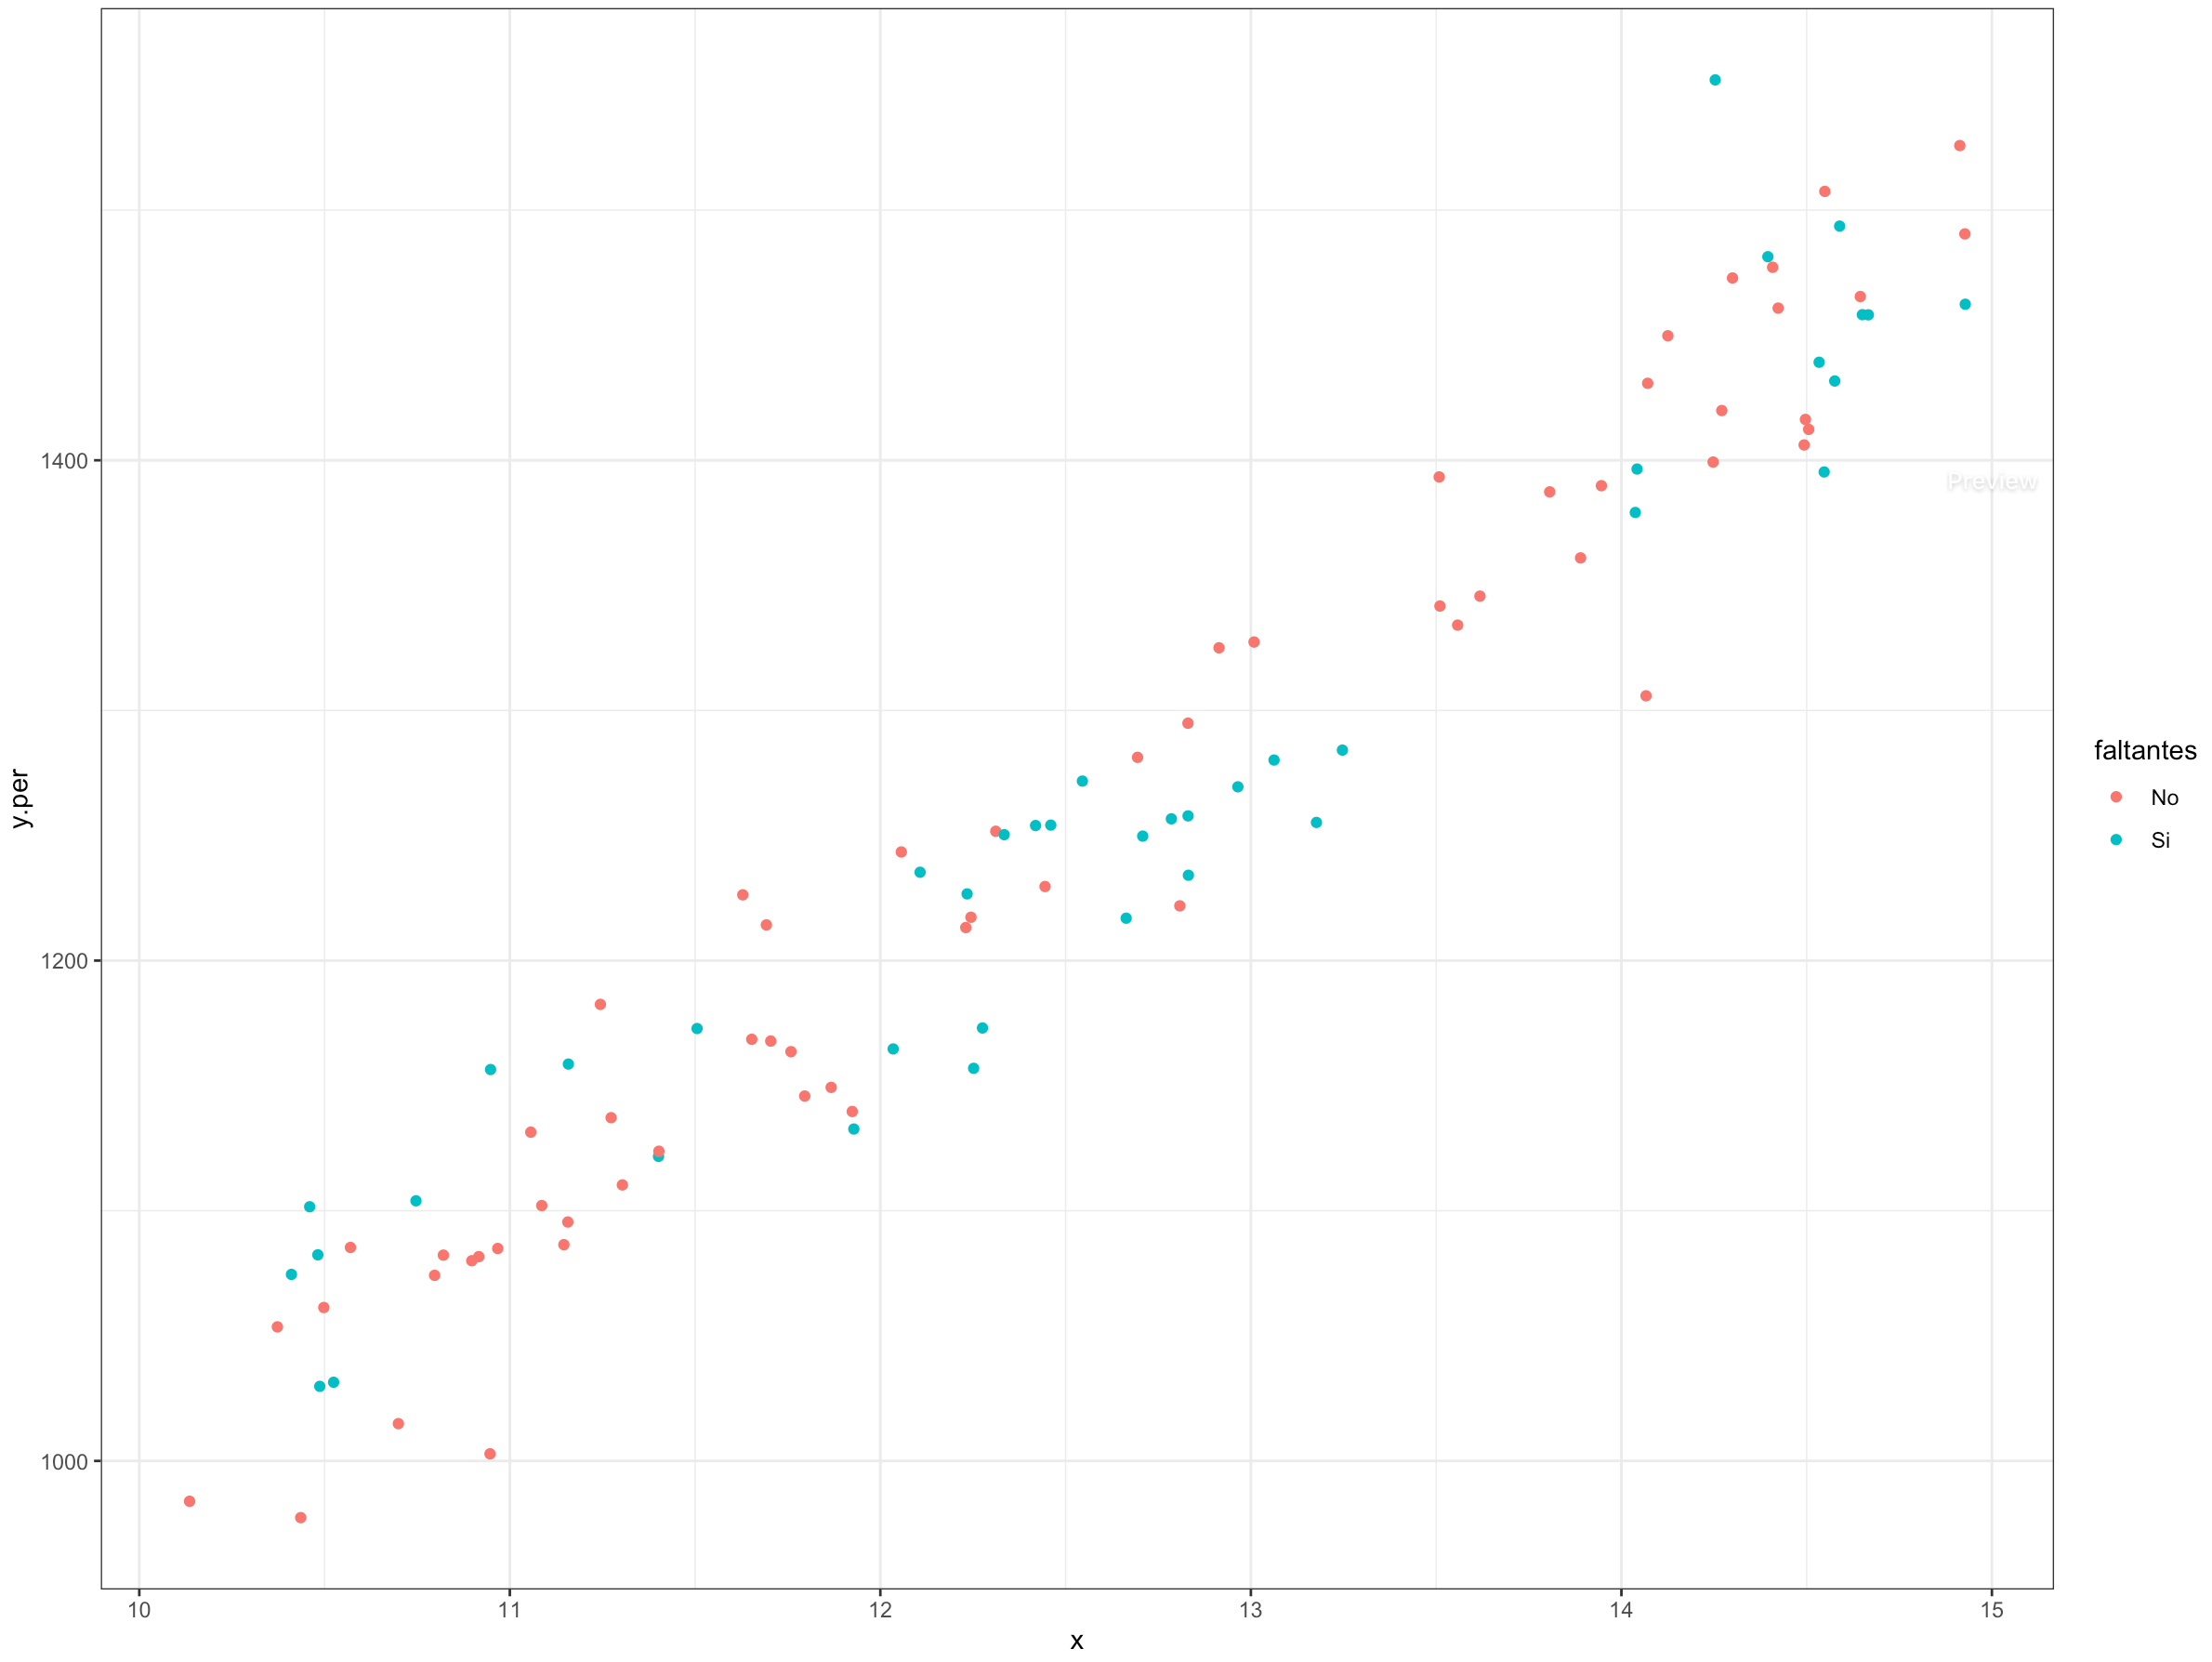
\includegraphics[width=0.5\linewidth]{Pics/im3} \caption{Relación de la variable de interés con la covariable auxiliar para el enfoque de imputación múltiple Bootstrap}\label{fig:figim3}
\end{figure}

Por otro lado, bajo distribuciones previas no informativas, es bien sabido que la distribución posterior de \(\sigma^2\) es:

\[
\sigma^2| y, x  \sim \frac{\sum_{i = 1}^{n_1} (y_i - \hat{\beta} x_i)^2}{\chi ^2_{n_1-1}}
\]

con \(\hat{\beta} = \frac{\sum_{i = 1}^{n_1} x_i y_i}{\sum_{i = 1}^{n_1} x_i^2}\). Asimismo, la distribución posterior de \(\beta\) es:

\[
\beta | \sigma^2, y, x \sim Normal \left(\hat{\beta}, \frac{\sigma^2}{\sum_{i = 1}^{n_1} x_i^2} \right)
\]

Asumiendo el anterior enfoque bayesiano de imputación múltiple, se llega a resultados similares. En ambos casos existe una buena dispersión en los valores imputados, respetando la distribución natural de la característica de interés. La siguiente gráfica así lo demuestra.

En resumen, a partir de esta simulación de Monte Carlo, se concluye rápidamente que imputar de manera determinista puede conllevar a la subestimación de la dispersión de la variable de interés. La siguiente tabla muestra que los tres métodos de imputación arrojaron estimaciones puntuales insesgadas. Sin embargo, el error estándar de la estimación simple es gravemente subestimado. De esta forma, la amplitud de los intervalos de confianza al 95\% inducidos por la estimación simple es inferior al de los otros dos métodos, causando que la cobertura del método simple sea deficiente, pues su nivel nominal en realidad no es del 95\%, sino del 83\%.

\begin{longtable}[]{@{}cccc@{}}
\toprule()
Propiedades & Ingenuo & Bootstrap & Bayesiano \\
\midrule()
\endhead
Esperanza & 100.00 & 100.01 & 100.01 \\
Error estándar & 0.24 & 0.41 & 0.42 \\
Amplitud & 0.96 & 1.60 & 1.66 \\
Cobertura & 0.83 & 0.97 & 0.95 \\
\bottomrule()
\end{longtable}

\hypertarget{detecciuxf3n-de-datos-atuxedpicos}{%
\chapter{Detección de datos atípicos}\label{detecciuxf3n-de-datos-atuxedpicos}}

En esta sección se describen los aspectos teóricos y prácticos de la identificación de valores atípicos en una base de datos completa (incluso con registros que ya han sido imputados), basándose en métodos que han mostrado buenas propiedades en la inferencia de encuestas de hogares. Después de una breve introducción, se presenta un enfoque no exhaustivo del problema de la identificación de valores atípicos, así como la teoría detrás de los métodos y algunos hallazgos empíricos de la imputación de valores atípicos.

Luego de detectar los posibles valores atípicos, el investigador debe enfrentarse al problema de decidir qué hacer con ellos; en general hay tres posible soluciones: mantenerlos en la base de datos final (sin ningún cambio), corregirlos (verificar exhaustivamente en los registros y cuestionarios, encontrar el error en la captura y reemplazarlo por el valor verdadero), o imputarlos (eliminarlos y reemplazarlos por un valor adecuado que no fue provisto por el respondiente). El enfoque de imputación de valores atípicos sigue los mismos principios que los método utilizado para imputar registros en el capítulo anterior. Al final, se recomienda que cuando se encuentren valores atípicos, se marquen para su revisión. Cuando se revisan, es posible encontrar que el valor es simplemente erróneo, debido a algún problema en la captura de los datos datos (error de medición); también es posible que el valor sea improbable y raro, pero que corresponda a un valor válido. En el primer caso el error se corrige (si el valor atípico es erróneo) y las estimaciones se ajustan. Si el valor atípico corresponde a un dato erróneo y no se puede localizar al encuestado, se recomienda imputarlo.

Por tanto, estamos interesados en detectarlos, y en solucionar el problema reemplazando los valores inverosímiles por otros más realistas. Detectar valores atípicos y distinguir aquellos que son errores de aquellos que son inusualmente altos (o bajos) pero valores correctos, es un desafío. Hacer estas
correcciones en los microdatos (es decir, en los datos a nivel del hogar) se suma al desafío. En general, un valor atípico es una observación que está distante de todos las demás observaciones o datos en la variable de interés de la base de datos.

Así como los valores erróneos deben corregirse, eliminarse o imputarse, por otro lado, se deben mantener los valores improbables en el conjunto de datos y se debe tomar una decisión para reducir su impacto en el análisis de la encuesta. Hay que tener en cuenta que existen valores verídicos en las observaciones que, aunque tienen una incidencia baja, deben conservarse en el análisis. Los valores que se apartan de la distribución habitual pueden clasificarse como valores atípicos o como puntos influyentes. El tratamiento de estos valores para el análisis vendrá definido por su clasificación.

\begin{itemize}
\tightlist
\item
  \emph{Valores atípicos representativos}: valores que se han registrado correctamente y representan otras unidades de población con valores similares.
\item
  \emph{Valores atípicos no representativos}: registrados incorrectamente o únicos, lo que significa que no hay otra persona como ellos.
\item
  \emph{Puntos de influencia}: cuando el efecto conjunto del punto de datos atípicos y su respectivo peso muestral tienen un efecto significativo en la inferencia.
\end{itemize}

A menudo, los valores atípicos pueden ser representativos de otros en la población, por lo que siguen siendo importantes y deben permanecer en el conjunto de datos. Al final, el proceso de identificación de valores atípicos se trata de un compromiso entre el sesgo y la varianza. Los valores atípicos pueden tener un gran impacto en los estimadores de ubicación y escala, como la media y la varianza, así como en los estimadores de totales y tamaños de subpoblaciones. Aunque estos estimadores permanecen insesgados, su varianza crece en presencia de valores atípicos.

\hypertarget{algunos-muxe9todos-de-detecciuxf3n-de-valores-extremos}{%
\section{Algunos métodos de detección de valores extremos}\label{algunos-muxe9todos-de-detecciuxf3n-de-valores-extremos}}

\citet{Filzmoser_Gussenbauer_Templ_2016} afirma que en el proceso de entrada de datos se pueden cometer errores. Por ejemplo, la introducción de valores de gasto imposibles, es decir, valores que son demasiado altos o demasiado bajos para ser plausibles. Estos valores extremos pueden tener un impacto significativo en algunos análisis particulares (como por ejemplo en el estudio de indicadores de desigualdad, o ajuste de modelos de regresión) que pueden verse significativamente afectados por un número reducido de valores influyentes en el conjunto de datos. En esta sección se realizará un recorrido no exhaustivo sobre algunos métodos para detectar valores extremos.

\hypertarget{muxe9todo-top-down}{%
\subsection{Método Top-Down}\label{muxe9todo-top-down}}

Suponga que \(y_{(1)}\le\cdots\le y_{(n)}\) denota los valores ordenados de la variable de interés \(y\) en la muestra \(s\). Considerando el total de la variable de interés para todos los elementos en la muestra, se define el porcentaje de contribución acumulado \(P_j\) de la siguiente manera:

\[
P_j=100\times\frac{\sum_{i=j}^n y_{(i)}}{\sum_{k=1}^n y_k}; \ \ \ \ \ \ \ j = 1, \ldots, n.
\]

Grandes cambios entre los valores de \(P_j\) significan posibles valores atípicos. También es posible calcular esta medida incluyendo el peso de muestreo para localizar qué valores ponderados tienen efectos anormalmente grandes.

\[
P_j^*=100\times\frac{\sum_{i=j}^n d_i \ y_{(i)}}{\hat t_{y, \pi}}; \ \ \ \ \ \ \ j = 1, \ldots, n.
\]

\hypertarget{muxe9todo-de-boxplot}{%
\subsection{Método de boxplot}\label{muxe9todo-de-boxplot}}

Uno de los métodos más básicos para identificar valores atípicos es construir un diagrama de caja utilizando la mediana y el rango intercuartílico \((RIC)\) de la variable de interés. En primer lugar, se define su \(RIC = Q_3 - Q_1\) y su mediana como \(m=Q_2\). Por consiguiente, un elemento se marcará como un valor atípico si cae fuera del siguiente intervalo:

\[
(m-c \times RIC,\ m+c \times RIC)
\]
En donde \(c\) es una constante predeterminada por el investigador, usualmente fijada entre 1.5 y 3.

\hypertarget{transformaciuxf3n-de-box-cox}{%
\subsection{Transformación de Box-Cox}\label{transformaciuxf3n-de-box-cox}}

Si la distribución de la variable es sesgada (como usualmente lo son los ingresos y gastos), es útil transformar la distribución para lograr una distribución simétrica antes de determinar los posibles valores atípicos. La transformación de Box-Cox se tiene la siguiente forma:

\[
y(\lambda)=
\left\{
\begin{matrix}\frac{y^\lambda-1}{\lambda},\; si\ \lambda\neq0,\\
log(y),\;si\ \lambda=0
\end{matrix}\right.
\]

En donde \(\lambda\in(-5,5)\). De esta forma, un ordenador iterará entre cada posible valor de \(\lambda\) para encontrar el que mejor reproduzca una distribución normal. Con esta nueva distribución, se puede utilizar el criterio de decisión de boxplot.

\hypertarget{muxe9todo-de-distancia-estandarizada}{%
\subsection{Método de distancia estandarizada}\label{muxe9todo-de-distancia-estandarizada}}

La transformación anterior solo funciona para valores positivos. El siguiente método muestra otra forma de transformar y estandarizar los datos. Suponga que \(z_k=w_ky_k\); si \(m_z\) es una estimación para la ubicación de \(z\), y \(\sigma_z\) es una estimación para la escala de \(z\). Entonces, la distancia estandarizada puede entonces definirse como

\[
\delta_{z_k}=\frac{z_k-m_z}{\sigma_z}
\]

De forma similar al método de boxplot, los registros se clasificaran como valores atípicos si el valor absoluto de \(\delta_{z_k}\) es mayor que un umbral predeterminado (normalmente 3). La media y la varianza de la muestra se pueden utilizar para las estimaciones de ubicación y escala para \(z_k\), pero no son robustas, ya que incluirán los valores atípicos potenciales, lo que a su vez reduce la probabilidad de que se identifiquen correctamente los registros atípicos. Por consiguiente, es posible utilizar estimadores robustos (resistentes a valores atípicos) para \(m_z\) y \(\sigma_z\), como por ejemplo la mediana y el rango intercuartílico de \(z_k\), respectivamente.

\hypertarget{muxe9todo-de-hidiroglou-bertholot}{%
\subsection{Método de Hidiroglou-Bertholot}\label{muxe9todo-de-hidiroglou-bertholot}}

Es posible utilizar una distancia estandarizada para detectar si la relación entre dos variables \(x\) y \(y\) en una unidad de la muestra difiere estructuralmente de las otras unidades en la muestra. Este método utiliza la idea de distancia estandarizada y también incorpora una medida de importancia para el tamaño de la unidad, con el fin de determinar el umbral para considerar un registro como un valor atípico. El algoritmo de identificación sigue los siguientes pasos:

\begin{enumerate}
\def\labelenumi{\arabic{enumi}.}
\tightlist
\item
  Para cada elemento calcular \(r_k=y_k/x_k\) para \(k\in s\).
\item
  Transformar los datos para poder detectar valores atípicos en cualquier extremo de la distribución. Los datos transformados están dados por:
  \[s_k=\left\{\begin{matrix}1-\frac{med(r_k)}{r_k},\;\ si\ 0\le r_k\le m e d(r_k)\\\frac{med(r_k)}{r_k}-1,\;\ en \ otro \ caso\\\end{matrix}\right.\] En donde \(med(r_k)\) corresponde a la mediana de los cocientes definidos en el paso anterior.\\
\item
  Incorporar la magnitud de los datos calculando los efectos \(E_k\) dados por
  \[
  E_k = s_k  \left( \max(x_k,y_k) \right)^\phi
  \]
  El parámetro \(\phi\) proporciona una medida de control para el impacto del tamaño en el efecto.
\item
  A continuación, calcular el primer, segundo y tercer cuartil de los efectos dados por \(E_{Q_1}, \ E_{Q_2}, \ E_{Q_3}\), respectivamente.
\item
  Los rangos intercuartílicos se calculan entonces como
  \[
  d_{Q_1} = \max\left(E_{Q_2} - E_{Q_1}\ , \ |0.5 \times E_{Q_2}|\right)
  \]
  \[
  d_{Q_3} = \max\left(E_{Q_3} - E_{Q_2}\ , \ |0.5 \times E_{Q_2}|\right) 
  \]
\end{enumerate}

Nótese que la cantidad \(|0.5*E_{Q_2}|\) es utilizada para reducir la tendencia a declarar falsos valores atípicos. Por ejemplo, esto ayudaría si la mayoría de los valores estuvieran agrupados alrededor de un valor particular, con unos pocos registros desviándose de él. Por último, los registros son declarados como valores atípicos si el valor de su efecto \(E_k\) queda fuera del intervalo \((E_{Q_2} - c \times d_{Q_1} \ , \ E_{Q_2} + c \times d_{Q_3})\); en donde al igual que en el método de boxplot, \(c\) controla el ancho de la región de aceptación.

\hypertarget{muxe9todo-de-la-distancia-de-mahalanobis}{%
\subsection{Método de la distancia de Mahalanobis}\label{muxe9todo-de-la-distancia-de-mahalanobis}}

Este método tiene en cuenta la estructura multidimensional de los datos observados en todos los registros comunes de un mismo módulo; por ejemplo, en el módulo de ingresos del hogar en una encuesta de hogares, o en el módulo de gastos de una encuesta de presupuestos familiares. En primer lugar, se supone que \(\mathbf{y}_k = (y_{k1}, y_{k2}, \ldots, y_{kQ} )'\) define el vector de valores observados del individuo \(k\) en todas las \(Q\) variables del módulo de interés. Por tanto, la distancia de Mahalanobis para una unidad se puede definir como
\[
MD_k^2=(\mathbf{y}_k-\bar{\mathbf{y}})' \ \mathbf{S}^{-1} \ (\mathbf{y}_k-\bar{\mathbf{y}})
\]

En donde \(\bar{\mathbf{y}}\) y \(\mathbf{S}\) son respectivamente el vector de medias muestrales y la matriz de covarianzas de las \(Q\) variables en el módulo. Si los datos siguen una distribución normal multivariante, se puede demostrar que la distribución de esta distancia es Ji-cuadrado con \(Q\) grados de libertad, \(MD_k^2 \sim \chi_Q^2\). A continuación, las unidades se declaran como potencialmente atípicas si superan el umbral del percentil 0.95 de la distribución \(\chi_{Q}^2\).

\hypertarget{la-distancia-de-cook}{%
\subsection{La distancia de Cook}\label{la-distancia-de-cook}}

Los registros influyentes son valores atípicos que afectan significativamente a los modelos de regresión. Para ubicarlos, es posible utilizar la distancia de Cook, que mide cuánto impacta la unidad \(i\)-ésima en la estimación de la unidad \(j\)-ésima, en un modelo de regresión con \(p\) variables explicativas. Esta medida está dada por la siguiente expresión:

\[
DC_{(i)} = \dfrac{\sum_{\substack{j=1\\ j\neq i}}^{n}(\hat y_j- \hat y_{j(i)})^2}{(p+1) \hat{\sigma}^2} 
\]

En donde \(\hat{\sigma}^2 = \frac{\sum_k (\varepsilon_k - \bar{e})^2}{n-p}\) es la varianza de los residuales del modelo \((\varepsilon_k)\); además, \(\hat y_j\) es la estimación de la \(j\)-ésima unidad en el modelo de regresión ajustado con todos los datos observados, mientras que \(\hat y_{j(i)}\) es la estimación de la \(j\)-ésima unidad cuando se excluye la \(i\)-ésima unidad. Entre más grande sea el valor de la estadística, es más probable que la observación de la unidad \(i\) se considere como un valor influyente. Algunos autores afirman que cualquier valor \(DC_{(i)}\) mayor que uno debe considerarse influyente, mientras que otros afirman que el umbral debe ser \(4/n\) o \(4/(n-p-1)\).

\hypertarget{el-criterio-dfbetas}{%
\subsection{El criterio DFBETAS}\label{el-criterio-dfbetas}}

Por otra parte, el estadístico DFBETAS mide cuánto influye la observación \(i\)-ésima en los estimadores de los coeficientes de regresión en un modelo lineal. La estadística se puede escribir como sigue:

\[
DFBETAS_{j(i)} = \dfrac{b_j-b_{j(i)}}{\sqrt{S^2_{(i)}C_{jj}}} 
\]

En donde \(b_j\) es la estimación para el \(j\)-ésimo coeficiente de regresión, \(b_{j(i)}\) es la estimación calculada sin la observación \(i\)-ésima; además \(S^2_{(i)}\) es la varianza muestral de la variable de interés sin la observación \(i\)-ésima y \(C_{jj}\) es el \(j\)-ésimo elemento de la diagonal de la matriz \((\mathbf x' \mathbf x)\), de dimensión \(n\times n\). Es posible considerar que cualquier cifra cuyo valor absoluto sea mayor o igual que \(2/\sqrt n\) determina que el valor atípico es influyente.

\hypertarget{ejemplo-detecciuxf3n-de-valores-atuxedpicos-en-una-encuesta-de-presupeustos-familiares-y-gastos}{%
\section{Ejemplo: detección de valores atípicos en una encuesta de presupeustos familiares y gastos}\label{ejemplo-detecciuxf3n-de-valores-atuxedpicos-en-una-encuesta-de-presupeustos-familiares-y-gastos}}

En genral, para cualquier tipo de encuesta, a la hora de detectar valores atípicos podría considerarse la estructura multivariante de los datos (relación con otras variables) en la búsqueda de valores atípicos. Para esto se debería elegir un conjunto de covariables de acuerdo con el juicio de los expertos y la desagregación necesaria. A pesar de que en la base de datos existan registros y valores observados para una observación, es posible que, después de la detección de valores atípicos, toda la información de una unidad sea declarada sospechosa. Por ende, una vez que se ha detectado una unidad con valores atípicos potenciales, es posible decidir que todos sus registros sean eliminados (creando deliberadamente una ausencia de respuesta de unidad) de no comprobarse la fiabilidad de la información. Por consiguiente, si se mantiene la unidad, toda su información se declara como confiable y valdrá la pena analizarla. De lo contrario, el registro se eliminará de los datos de la muestra que afectan la estructura del esquema de ponderación. Luego, la unidad se declarará como una unidad eligibles no respondientes (ENR, ver capitulo 10).

Después de decidir acerca de los valores atípicos de la unidad, es necesario detectar los valores atípicos de los registros para las variables específicas de la encuesta. Por ejemplo, en una encuesta de presupuestos familiares, las variables de interés serán los rubros asociados a los ingresos y a los gastos del hogar. En este caso, se sugiere que la variable de interés de una categoría particular se transforme utilizando el enfoque de Box-Cox. Esto se hace porque las distribuciones de ingresos y gastos siempre están sesgadas. Una vez transformados, es posible utilizar las medidas anteriormente mencionadas para decidir acerca de la eliminación del registro. Por ejemplo, si dos o tres de los métodos detectan un registro como un posible valor atípico, entonces se verifica la información sobre ese registro. Si la información del elemento es sospechosa, se debe eliminar y utilizar un enfoque de imputación sobre ese registro.

Siguiendo con el esquema de la encuesta de presupuestos familiares, podría ser conveniente que, a nivel de gasto, la detección de los valores atípicos se realizara, no sobre cada artículo, sino a nivel agregado para cada nivel de la clasificación de consumo (COICOP, \emph{Classification of Individual Consumption According to Purpose}). Además se deben tener en cuenta que, en este tipo de encuestas, los valores nulos para el gasto o consumo de artículos particulares son frecuentes, ya que no se puede esperar que todos los hogares consuman todos los artículos posibles. Estos valores cero se denominan \emph{ceros estructurales}. Por ende, es muy pertinente estudiar y decidir si la metodología de detección de valores atípicos tendrá en cuenta los ceros o no. En general, cuando la incidencia de los ceros es baja no debería existir ningún inconveniente en analizar el conjunto de datos incluyendo estos ceros. Por ende, esta decisión debería ser independiente para cada división.

Para algunos componentes concretos, el número de ceros puede ser bastante alto y los algoritmos de detección de valores atípicos pueden fallar si el número de ceros está por encima de un determinado umbral. Las observaciones podrían incluso convertirse en valores atípicos debido a los ceros cuando se aplican métodos de detección. En este sentido, es necesario contemplar umbrales flexibles para cada división. Por ejemplo, un valor de cero en los gastos de alimentos sería poco realista, pero podría ser cierto para los gastos en ropa de bebé o muebles. Por las anteriores razones, es plausible recomendar la agregación de los componentes del consumo en grandes categorías a nivel de producto/servicio o grupos agregados de productos y servicios.

Un indicador fiable, no solo para medir la desigualdad en el consumo sino también para realizar un seguimiento de los cambios en el proceso de detección de valores atípicos y la imputación posterior, es el coeficiente de Gini. Por ejemplo, considere la siguiente tabla que muestra la presencia de ceros en cada división COICOP junto con el Gini para algunas de las categorías anteriormente mencionadas. Nótese que la incidencia de ceros es mucho menor en la categoría de vivienda que en las categorías de educación o recreación.

\begin{longtable}[]{@{}ccc@{}}
\toprule()
Categoría & Ceros & Gini \\
\midrule()
\endhead
Alimentos & 27 & 36 \\
Alcohol & 4333 & 90 \\
Ropa & 2558 & 78 \\
Vivienda & 5 & 48 \\
Muebles & 85 & 53 \\
Salud & 2746 & 78 \\
Transporte & 616 & 69 \\
TIC & 551 & 62 \\
Recreación & 3538 & 92 \\
Educación & 4802 & 90 \\
Restaurantes & 1421 & 65 \\
Seguros & 4837 & 90 \\
Cuidado personal & 129 & 51 \\
\bottomrule()
\end{longtable}

Esta metodología también se puede aplicar para grupos. La siguiente tabla muestra la presencia de ceros estructurales para algunos artículos de la sección Alimentos. Una vez más, dependiendo del país, sería esperable encontrar una mayor incidencia de ceros en algunos artículos. En este caso particular, nótese que hay una mayor cantidad de ceros en artículos como té o café, que en artículos como cereal, azúcar o leche.

\begin{longtable}[]{@{}ccc@{}}
\toprule()
Artículos & Ceros & Gini \\
\midrule()
\endhead
Cereales & 87 & 37 \\
Carne & 481 & 47 \\
Pescado & 305 & 56 \\
Leche & 290 & 47 \\
Aceites & 482 & 51 \\
Frutas & 981 & 67 \\
Verduras & 188 & 47 \\
Azucares & 290 & 56 \\
Comida procesada & 253 & 43 \\
Jugos & 3650 & 79 \\
Café & 5286 & 86 \\
Té & 4709 & 86 \\
Cacao & 4421 & 78 \\
Agua & 5287 & 86 \\
Refresco & 4859 & 86 \\
Otras bebidas & 3353 & 79 \\
\bottomrule()
\end{longtable}

Como se resaltó anteriormente, para datos muy sesgados, los métodos para la detección de valores atípicos podrían resultar problemáticos, ya que el intervalo en el que los puntos de datos no se consideran valores atípicos es simétrico alrededor de la mediana. Por ejemplo, la figura \ref{fig:figou2} muestra el comportamiento estructural de algunas divisiones, es notable que todas las distribuciones de gasto y consumo en estos conceptos están extremadamente sesgadas.

\begin{figure}
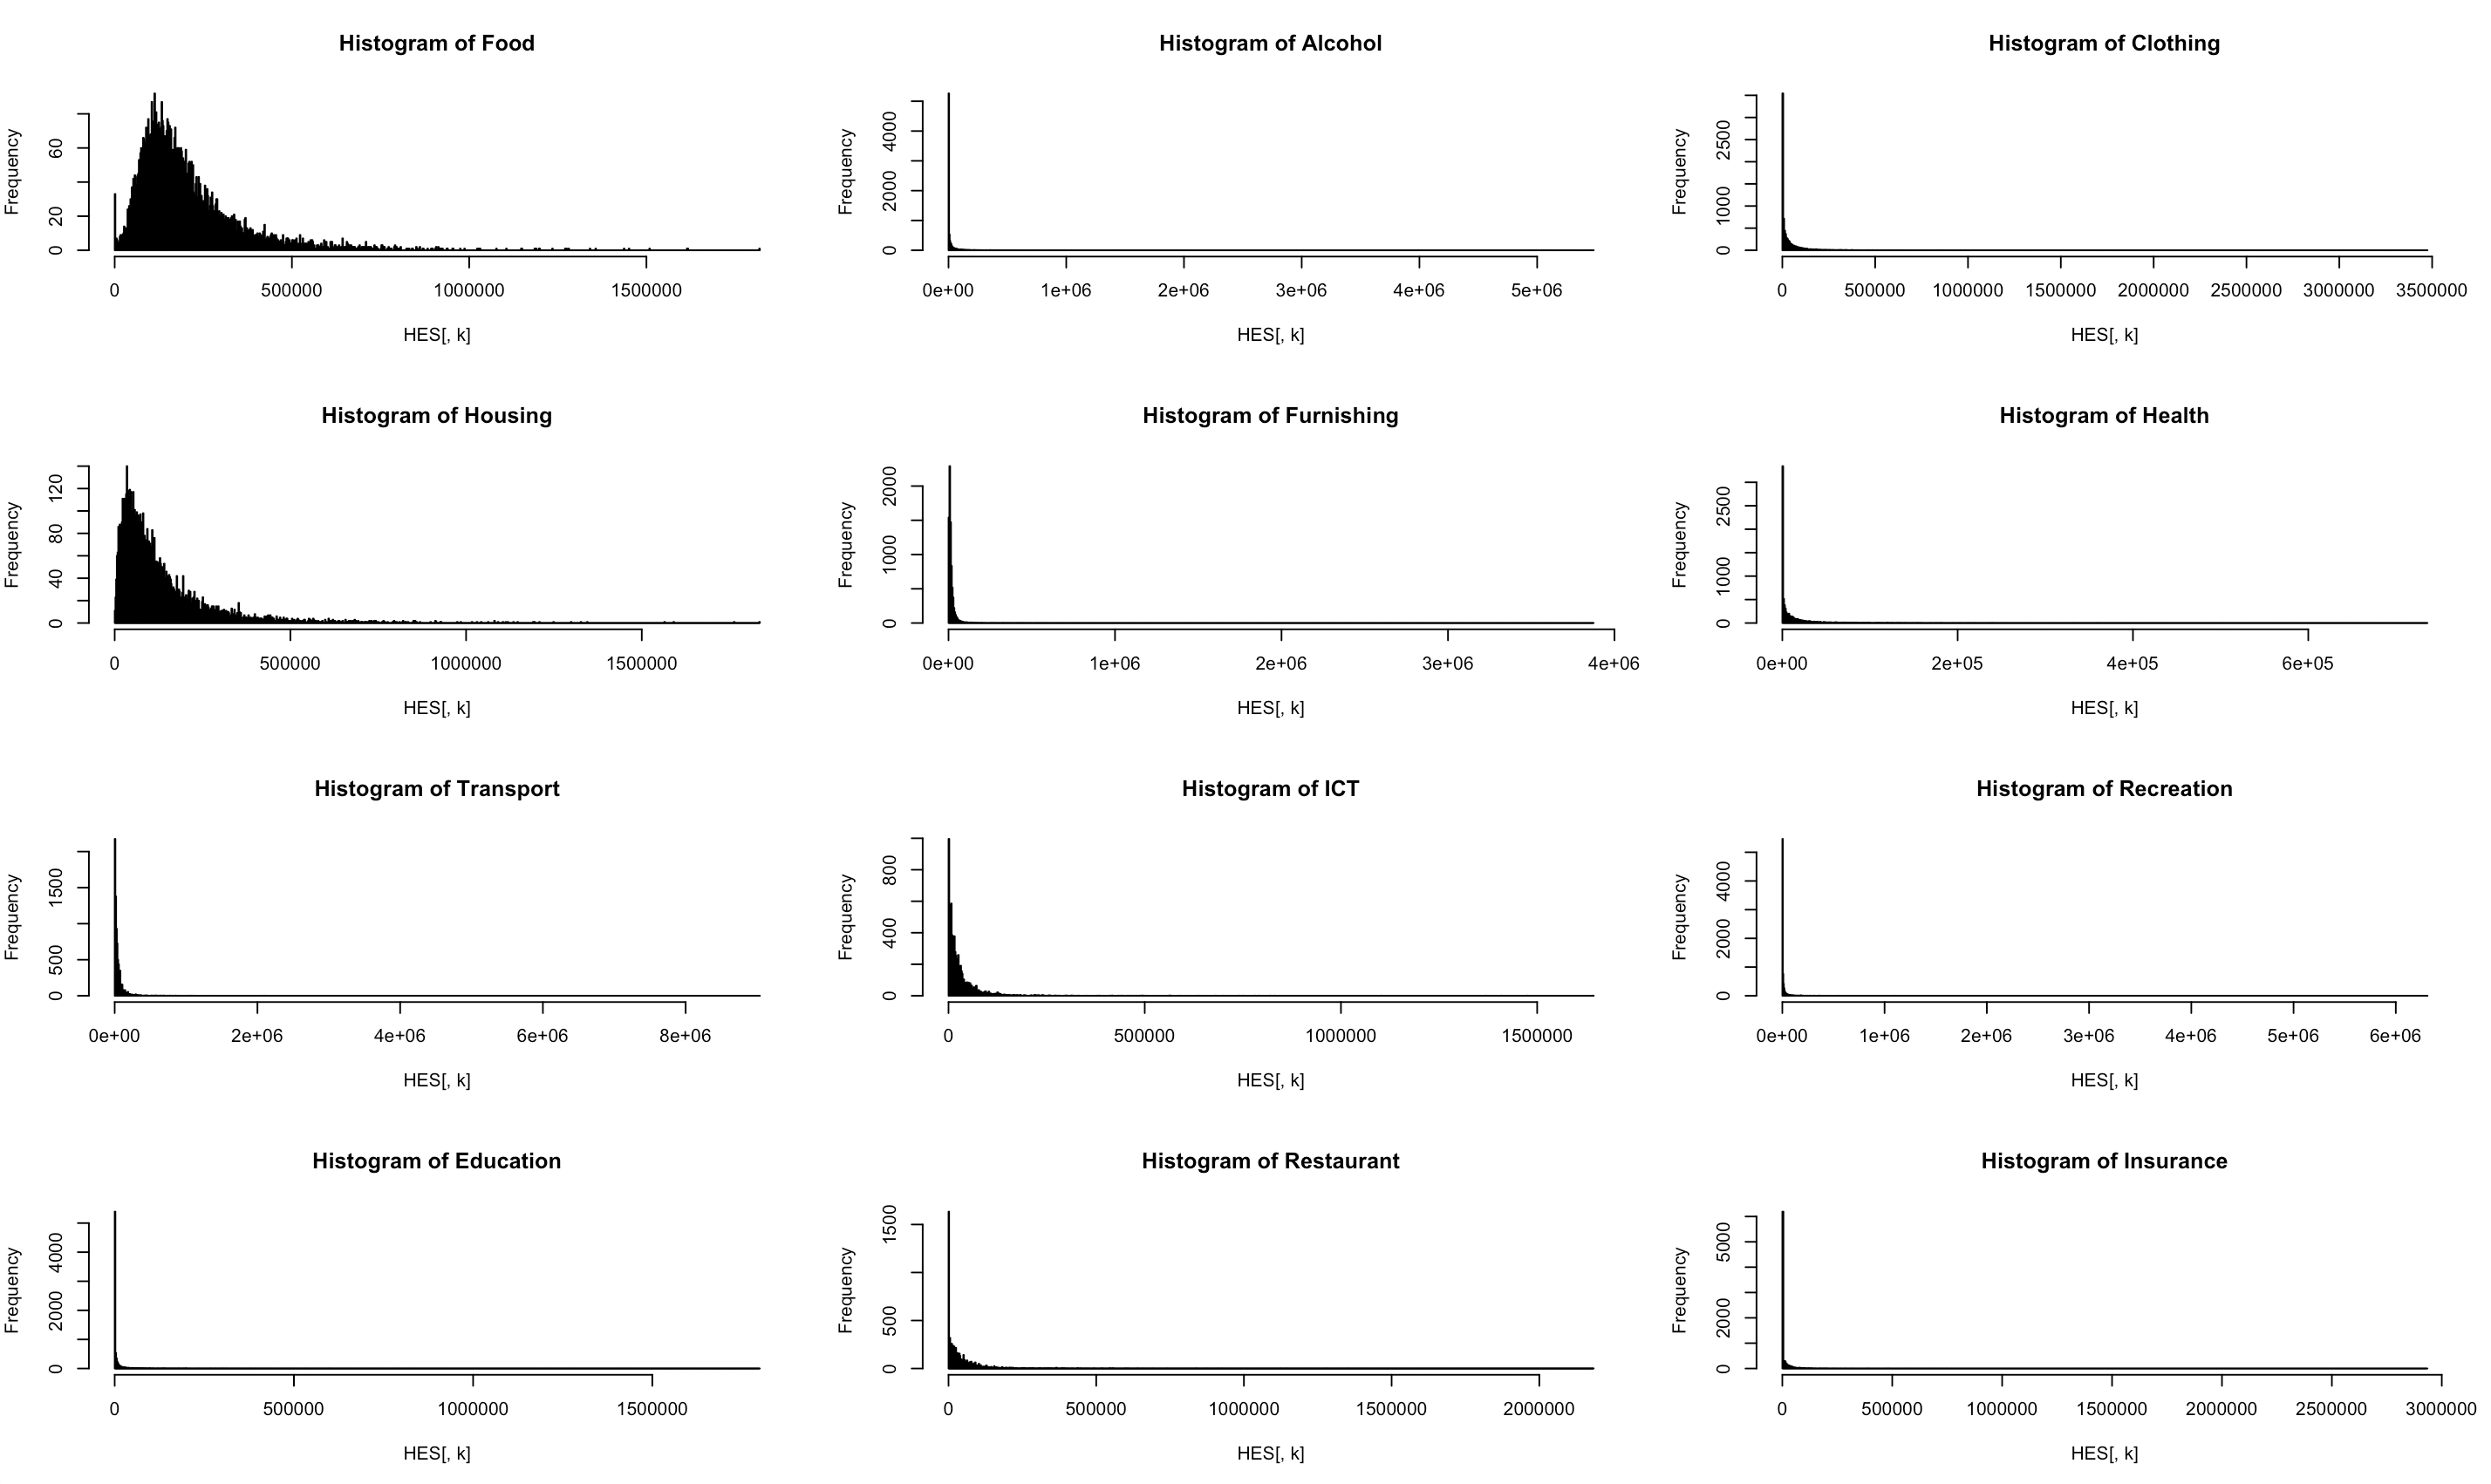
\includegraphics[width=0.5\linewidth]{Pics/ou2} \caption{Distribución del consumo para algunas categorías del gasto.}\label{fig:figou2}
\end{figure}

Para ajustarse a este problema es posible utilizar la transformación de Box-Cox con el fin de obtener una distribución simétrica para los datos antes de determinar los posibles valores atípicos. La figura \ref{fig:figou1} muestra el proceso de iteración de esta metodología en algunas divisiones. La línea vertical en cada gráfica corresponde al mejor valor que podría tomar \(\lambda\) para que los datos se ajusta a una distribución normal.

\begin{figure}
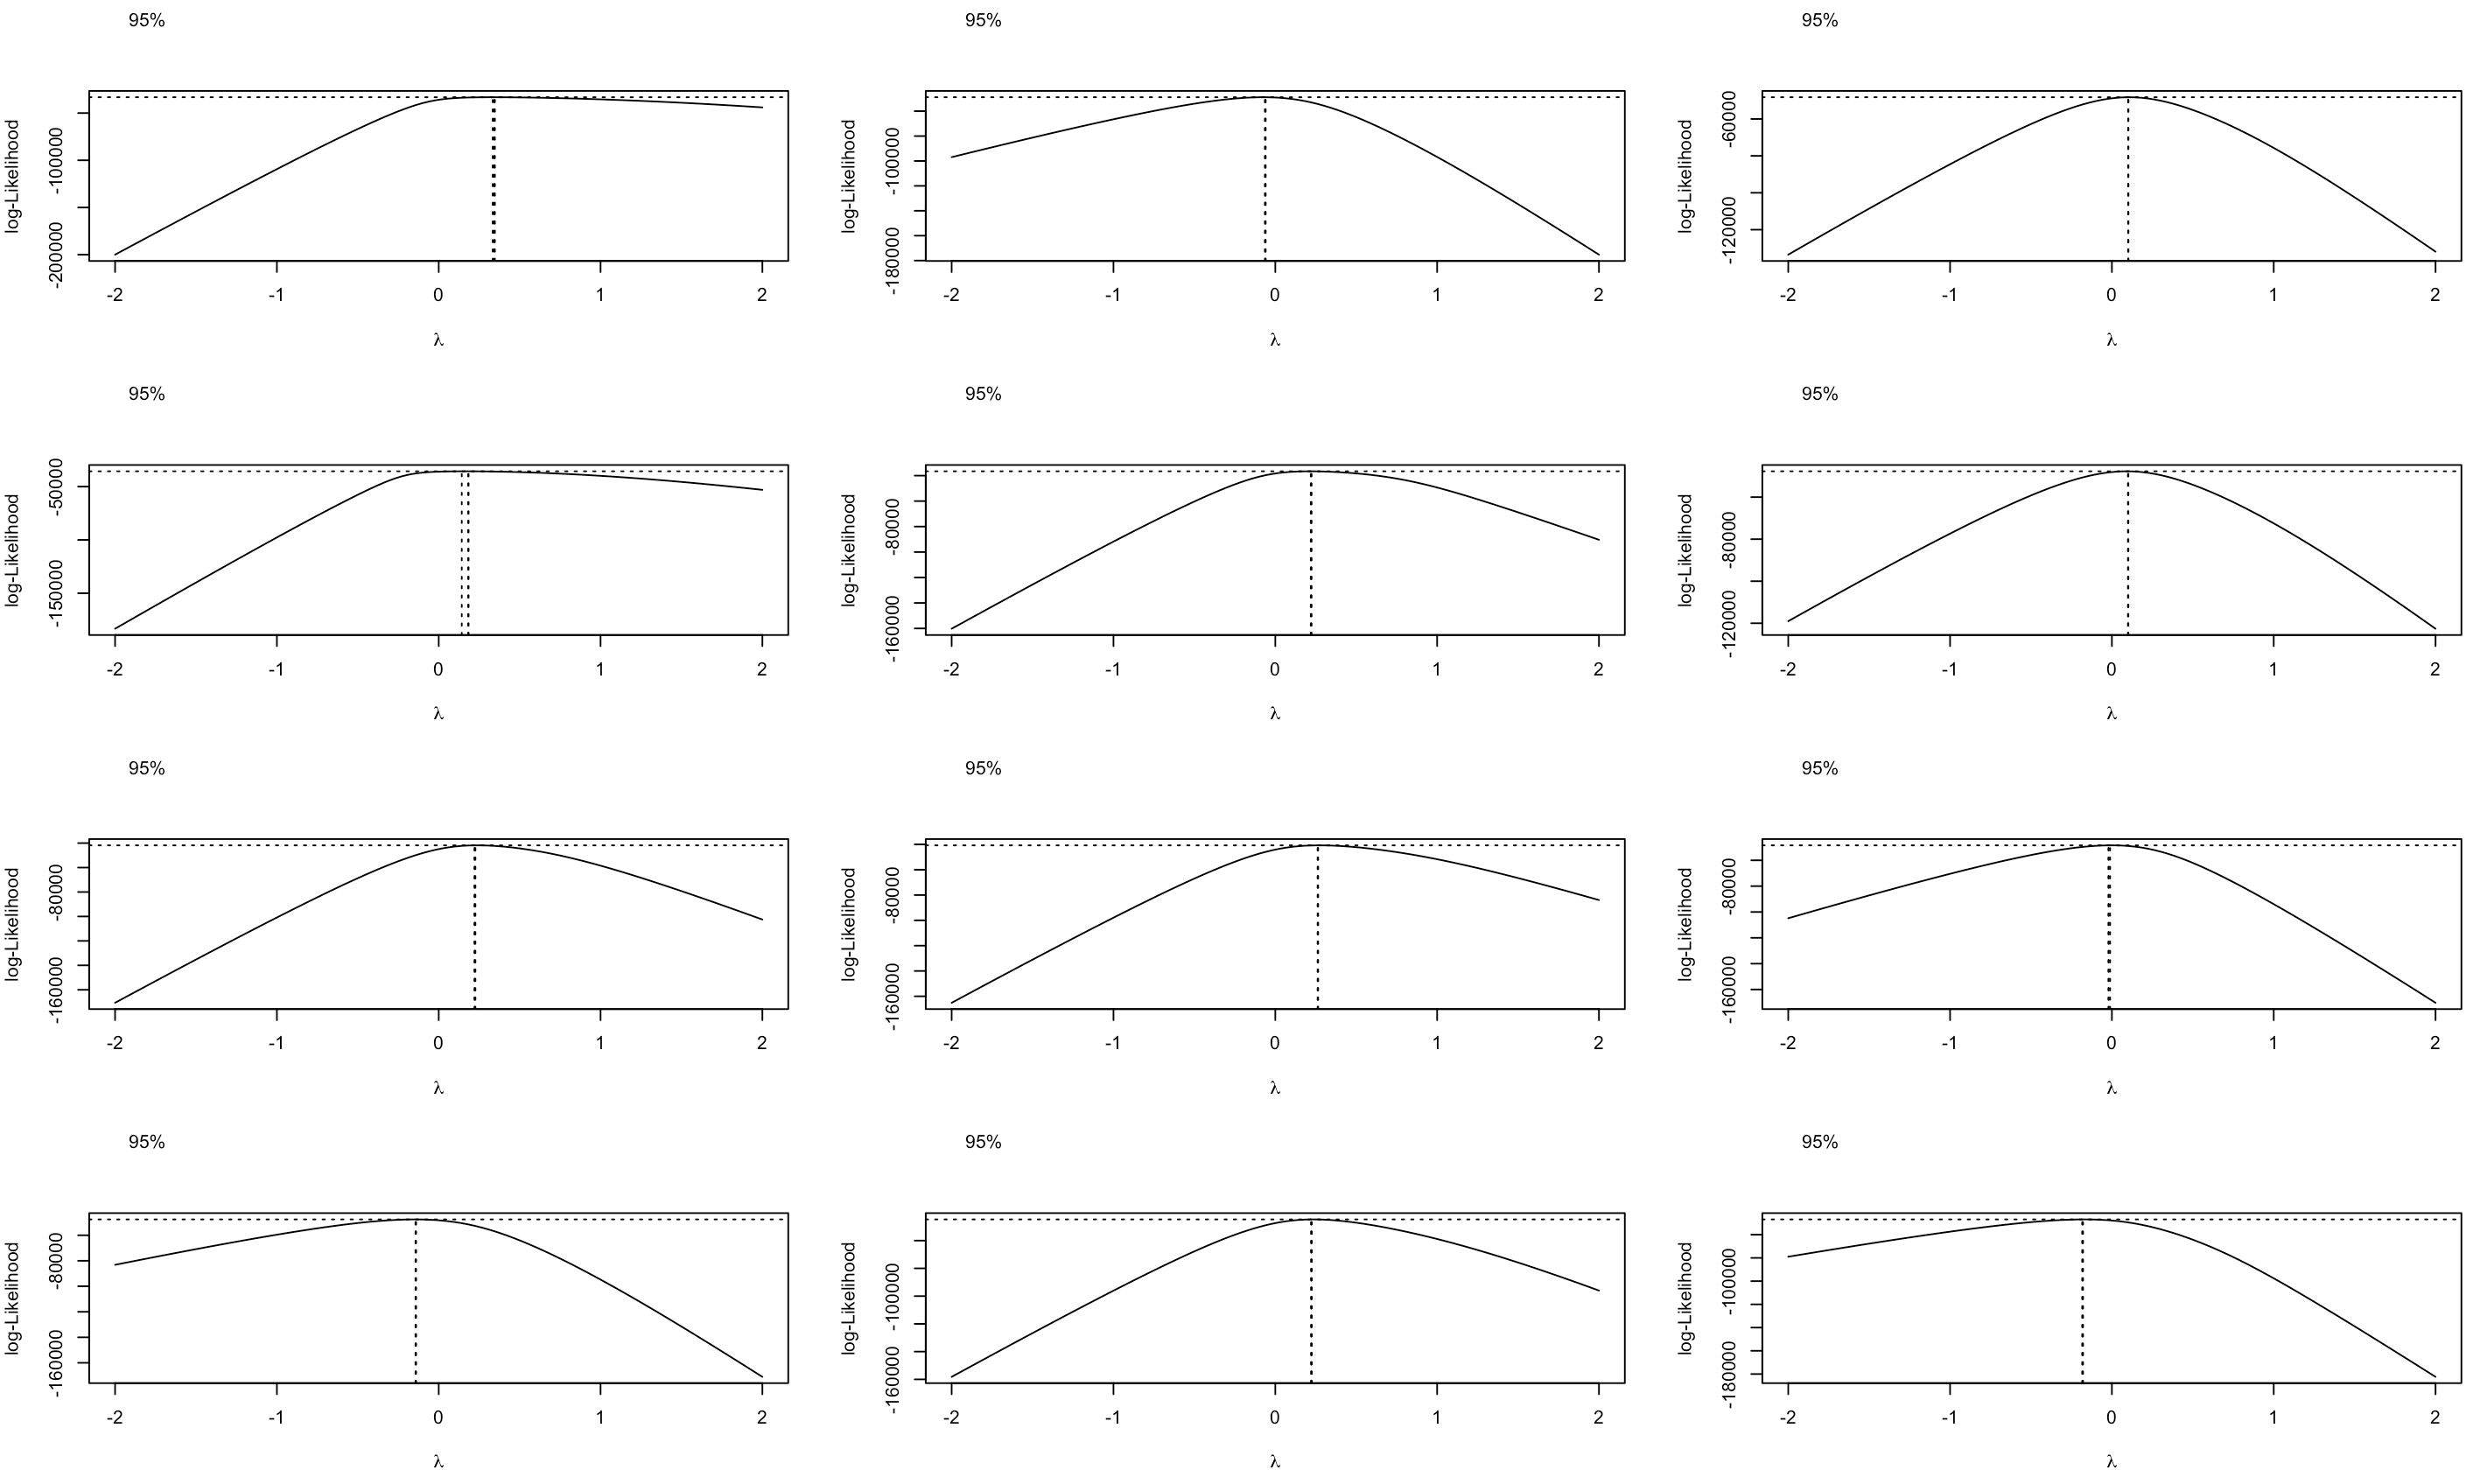
\includegraphics[width=0.5\linewidth]{Pics/ou1} \caption{Valores óptimos para las transformaciones de Box-Cox en algunas categorías del gasto.}\label{fig:figou1}
\end{figure}

Luego de haber transformado apropiadamente los datos, es posible utilizar la metodología de Boxplot, uno de los métodos más básicos (aunque muy poderoso), para identificar valores atípicos. Como se mencionó en la sección anterior, la gráfica mostrará el mínimo de la muestra, el primer cuartil, la mediana, el tercer cuartil y el máximo. La caja va del primer al tercer cuartil (que contiene por definición el 50\% de los datos más internos), así como la mediana que generalmente está marcada por una línea media. Para la aplicación específica de la detección de valores atípicos dentro de las divisiones COICOP es posible que la constante predeterminada \(c\) varíe entre divisiones. Por ejemplo, la siguiente tabla muestra el número de valores atípicos detectados en cada división por este método.

\begin{longtable}[]{@{}cc@{}}
\toprule()
División & Valores atípicos \\
\midrule()
\endhead
Alimentos & 222 \\
Alcohol & 0 \\
Ropa & 0 \\
Vivienda & 87 \\
Muebles & 330 \\
Salud & 0 \\
Transporte & 743 \\
TIC & 668 \\
Recreación & 0 \\
Educación & 0 \\
Restaurantes & 31 \\
Seguros & 0 \\
Cuidado personal & 400 \\
\bottomrule()
\end{longtable}

Por otro lado, también es posible tener en cuenta la relación entre el gasto en cada división y el ingreso reportado por el hogar en la encuesta. En general, no se puede suponer que esta relación es homogénea entre todos los encuestados, máxime si se tiene en cuenta que la selección de las unidades muestrales se hace en todos los grupos socioeconómicos del país. Sin embargo, sí es posible hacer este supuesto dentro de clases homogéneas, como por ejemplo el cruce entre los quintiles (o deciles) del ingreso y las regiones del país. De esta forma, dentro de cada grupo se supondría que la relación entre el gasto y el ingreso es uniforme. Por ejemplo, en la siguiente tabla se muestra el número de valores atípicos detectados en cada división mediante el método Hidiroglou-Bertholot.

\begin{longtable}[]{@{}cc@{}}
\toprule()
División & Valores atípicos \\
\midrule()
\endhead
Alimentos & 74 \\
Alcohol & 141 \\
Ropa & 73 \\
Vivienda & 53 \\
Muebles & 177 \\
Salud & 71 \\
Transporte & 89 \\
TIC & 128 \\
Recreación & 168 \\
Educación & 117 \\
Restaurantes & 48 \\
Seguros & 100 \\
Cuidado personal & 247 \\
\bottomrule()
\end{longtable}

Es necesario tener en cuenta que, como la lógica detrás de estos dos métodos difiere, cada uno identificará un número diferente de valores atípicos. Esto es una ventaja, porque los métodos son complementarios. Por ejemplo, en divisiones como ropa, vivienda, salud, recreación y educación, donde el método Boxplot no encontró ningún valor atípico posible, el método HB sí lo encontró. Es así como, teniendo en cuenta los resultados de estos dos métodos, se puede especificar una regla lógica para asignar una marca a los registros de la base de datos que deban ser revisados por considerarse sospechosos. Por ejemplo, es posible que haya categorías en las que la regla lógica sea una conjunción de los resultados de los métodos, mientras que podría haber otras en las que la regla lógica sea una disyunción entre los resultados.

Al final, se debe imputar cualquier valor que se considere como un valor atípico. Como se vio en los capítulos anteriores, la imputación puede estar apoyada por un enfoque basado en modelos. Por ejemplo, para imputar el gasto percápita anualizado, es posible utilizar el método de regresión con el vecino más cercano, donde se define un modelo lineal para las unidades encuestadas (sin incluir los valores atípicos). Una vez estimados los coeficientes de regresión, se calcula un valor previsto para esas unidades de valores atípicos y se identifica a un solo donante como el hogar cuyo gasto total en esa División está más cerca de la predicción. En la siguiente tabla se presentan algunos resúmenes de la distribución de los gastos a nivel de división antes de imputar los valores atípicos.

\begin{longtable}[]{@{}cccc@{}}
\toprule()
División & Mínimo & Mediana & Máximo \\
\midrule()
\endhead
Alimentos & 0 & 164587 & 1819370 \\
Alcohol & 0 & 0 & 5475960 \\
Ropa & 0 & 8180 & 3474000 \\
Vivienda & 0 & 89040 & 1835500 \\
Muebles & 0 & 10503 & 3871476 \\
Salud & 0 & 2400 & 735180 \\
Transporte & 0 & 24700 & 9038783 \\
TIC & 0 & 16125 & 1642500 \\
Recreación & 0 & 860 & 6307200 \\
Educación & 0 & 0 & 1800000 \\
Restaurante & 0 & 22100 & 2184000 \\
Seguro & 0 & 0 & 2932400 \\
Cuidado personal & 0 & 18540 & 1223734 \\
\bottomrule()
\end{longtable}

Por último, en la tabla que se muestra a continuación se examinan algunos resúmenes sobre la distribución de los gastos a nivel de división habiendo imputado los valores atípicos de forma diferencial y con independencia ne cada división. Se nota cómo la imputación pasa realmente cambia la perspectiva del consumo mínimo y máximo. Esto significa que la detección de valores atípicos se centró en ambos lados de la distribución del gasto.

\begin{longtable}[]{@{}cccc@{}}
\toprule()
División & Mínimo & Mediana & Máximo \\
\midrule()
\endhead
Alimentos & 4560 & 166280 & 1616504 \\
Alcohol & 0 & 0 & 930400 \\
Ropa & 0 & 8250 & 1446532 \\
Vivienda & 3000 & 89280 & 726000 \\
Muebles & 243 & 10730 & 279382 \\
Salud & 0 & 2400 & 654000 \\
Transporte & 60 & 29900 & 365000 \\
TIC & 0 & 16627 & 591000 \\
Recreación & 0 & 867 & 1054100 \\
Educación & 0 & 0 & 494000 \\
Restaurantes & 0 & 22133 & 520000 \\
Seguro & 0 & 0 & 723000 \\
Cuidado personal & 400 & 18855 & 658960 \\
\bottomrule()
\end{longtable}

\hypertarget{agregaciuxf3n-de-encuestas}{%
\chapter{Agregación de encuestas}\label{agregaciuxf3n-de-encuestas}}

Para producir indicadores sociales de forma agregada (anual, semestral o
trimestral), es común recurrir a la agregación de las bases de datos
provenientes de las encuestas de hogares, cuya periodicidad puede suele
ser mensual o trimestral. En esta sección se exploran algunas
estrategias de estimación ligadas al tratamiento de los pesos inducidos
por el diseño de muestreo complejo y al tratamiento de las unidades que
se repiten en algún periodo debido al carácter rotativo de la medición.

Uno de los primeros acercamientos al problema de la estimación conjunta
de indicadores sociales utilizando varios periodos de recolección se
presenta en \citet{Gurney_Daly_1965}, en donde se examina cómo mejorar el
estimador puntual por medio de la correlación natural que se tiene con
periodos anteriores, siguiendo un enfoque inferencial basado en modelos
estocásticos. En este orden de ideas, \citet{Lent_Miller_Duff_1999} definen una
aproximación a un estimador para las distintas clasificaciones de la
fuerza de trabajo que está basado en la optimización de los coeficientes
de un estimador compuesto.

Por su parte, \citet{Fuller_1990} provee una
discusión acerca de los sesgos que se pueden generar en el análisis de
encuestas repetidas debido a errores de medición y revisa detalladamente
algunos modelos estimados con mínimos cuadrados. Además, \citet{Bell_2001}
examina varios acercamientos al problema de estimar indicadores
sociales, específicamente relacionados con la fuerza de trabajo,
provenientes de encuestas de hogares que tienen definido un esquema de
rotación y traslape entre distintos periodos de tiempo.

Asimismo, \citet{Steel_McLaren_2008} revisaron las principales dificultades al
momento de diseñar y analizar encuestas repetidas. Teniendo en cuenta
los patrones de rotación en la estimación de los indicadores de nivel y
de cambio, examinan su efecto en la estrategia de estimación de las
varianzas de los estimadores de interés. Luego, \citet{Lewis_2017} definieron
algunos procedimientos que se deben seguir al momento de combinar dos o
más conjuntos de datos con el propósito de implementar eficientemente
pruebas de significación estadística sobre indicadores de cambio en el
tiempo, además de incrementar el tamaño de muestra para realizar
inferencias de subgrupos poblacionales que están insuficientemente
representados en una sola medición.

\hypertarget{esquemas-de-acumulaciuxf3n-de-muestras}{%
\section{Esquemas de acumulación de muestras}\label{esquemas-de-acumulaciuxf3n-de-muestras}}

Antes de entrar en los detalles técnicos involucrados en este tipo de
procedimientos, tomemos una situación ejemplificante específica para
ilustrar la problemática que se quiere abordad. Para esto, suponga que
un INE en América Latina ha previsto una
nueva forma de análisis de su encuesta de empleo. Con el fin de tener
representatividad a un nivel más desagregado (provincial, por ejemplo),
y para poder realizar una estimación más precisa, ha decidido realizar
una agregación anual de todos los levantamientos de su encuesta de
empleo. Por ejemplo, suponga que en los meses de marzo, junio,
septiembre y diciembre se planean levantamientos trimestrales y que este
esquema considera una representatividad nacional, en el área urbana y
rural, aunque no lo hacía con la representatividad provincial, ni de las
ciudades principales del país. Con la metodología de agregación de
muestras podría ser posible asegurar la representatividad en las
provincias desagregadas por área (urbano o rural).

Los procesos de acumulación de muestras son realizados con frecuencia en
las encuestas continuas con publicación trimestral. Por ejemplo, se
puede planear levantamientos mensuales y acumular tres meses para
realizar la publicación trimestral de la cifra de desempleo. De hecho,
algunos países han decidido publicar cifras mensuales del desempleo
teniendo en cuenta la acumulación de los últimos tres levantamientos, lo
que es conocido cono trimestres móviles. Teniendo en cuenta el diseño
rotativo que muchas encuestas implementan en América Latina, una de las
bondades de estos esquemas de agregación de muestras en los trimestres
móviles es que el panel original se mantiene y además, por diseño, la
misma vivienda no es entrevistada dos veces en el trimestre móvil. En
este tipo de diseños, inclusive es posible que, al final de cada año en
diciembre, se contemple la publicación de un gran agregado anual que
contemple la agregación de los doce meses anteriores. En este escenario
sí existen viviendas que han sido entrevistadas dos o más veces y este
porcentaje, dependiendo del diseño rotativo, puede no ser bajo. Por
ejemplo, en un panel 2(2)2, el diseño rotativo induce un traslape
natural del 50\% entre trimestres.

\citet[capítulos 7 y 8]{Korn_Graubard_1999} proveen un recuento exhaustivo
sobre las opciones de ponderación y otros temas a considerar cuando se
combinan datos a lo largo del tiempo en encuestas complejas. En el caso
de la agregación de muestras se resalta que todas las viviendas que han
sido entrevistadas en más de una ocasión deben pertenecer a la misma UPM
por diseño. Es muy importante que la identificación de las UPM y de los
estratos de muestreo se realice de manera inequívoca y se debe
asegurar que los siguientes principios se cumplan a cabalidad:

\begin{enumerate}
\def\labelenumi{\arabic{enumi}.}
\tightlist
\item
  Cuando se combinan dos o más oleadas del mismo panel es importante
  asegurarse que las UPM sean emparejadas correctamente, de tal forma
  que el software las reconozca como iguales.
\item
  Cuando se combinan dos o más muestras independientes es importante
  asegurarse que las UPM estén codificada de tal forma que el software
  las reconozca como distintas.
\end{enumerate}

Cuando se trata de estimar las varianzas de este tipo de estimadores,
los cálculos analíticos se tornan mucho más complicados.
\citet{Train_Cahoon_Makens_1978} muestran lo complicado que puede ser calcular
las variaciones de los promedios de las estimaciones de múltiples
períodos de tiempo en una encuesta repetida y cómo estos cálculos
dependen en gran manera del patrón de traslape definido en el diseño de
la encuesta. Para las encuestas de población activa, a menudo se utiliza
un enfoque computacional basado en métodos de remuestreo, como
\emph{Jackknife}, \emph{Bootstrap} o \emph{BRR}. Nótese que el uso apropiado de tales
métodos, también dependerá del origen de la encuesta y de sus objetivos.
Por ejemplo, los insumos de aplicación de los métodos serían unos si la
encuesta está orientada a medir el desempleo, y serían otros si la encuesta
está diseñada para estimar los cambios brutos entre dos periodos de
tiempo.

\hypertarget{factores-de-expansiuxf3n-y-estimadores-de-muestreo}{%
\section{Factores de expansión y estimadores de muestreo}\label{factores-de-expansiuxf3n-y-estimadores-de-muestreo}}

Si el investigador está interesado en estimar la tasa de
desempleo anual sobre una encuesta rotativa, que se lleva a durante los cuatro trimestres del año, es posible usar los cuatro conjuntos de datos y unir los trimestres para estimar la tasa de desempleo anual. Una solución
inicial a este problema consiste en agregar las cuatro bases de datos y
dividir los pesos de muestreo de cada periodo por un factor de cuatro.
El anterior procedimiento induce estimadores puntuales aproximadamente
insesgados, aunque las estimaciones de los errores estándar se tornan un
poco más complicadas, puesto que se debe concatenar exhaustivamente las
UPM (o incluso crear unidades de varianza).

Por supuesto, las encuestas que utilizan diseños rotativos, en donde un
hogar es entrevistado en varias ocasiones, deben adjuntar dos clases de
pesos de muestreo: los transversales y los agregados. Los pesos
transversales, discutidos en las secciones anteriores, son aquellos
inducidos por el diseño de muestreo de la encuesta en cada aplicación y
que permiten obtener estimaciones de los parámetros de interés de forma
periódica (mensual, trimestral o semestral). De esta forma, por ejemplo
en una encuesta de fuerza de trabajo, los datos transversales se usarán
para producir estimaciones periódicas de la participación en la fuerza
de trabajo, o de la tasa de pobreza, o de la tasa de desempleo, etc. Por ejemplo, la estimación de la tasa de desempleo usa
un estimador de razón, definido de la siguiente forma

\[\hat\theta=\frac{\sum_s d_ky_k}{\sum_s d_kz_k}\]

En donde, para la persona \(k\)-ésima, \(d_k\) representa su peso de
muestreo, \(y_k\) representa su estado de ocupación (específicamente,
\(y_k=1\) si la persona está desempleada) y \(z_k\) es su estado en la
fuerza de trabajo (específicamente, \(z_k=1\) si la persona pertenece a la
población económicamente activa). Esta estrategia de estimación asume que cada persona
se representa a sí misma y a otras más en la población. Nótese que los
pesos transversales asignados estarán determinados por la probabilidad
de selección de las UPM, la probabilidad de selección del hogar dentro
de la UPM, el ajuste por ausencia de respuesta en ese mismo mes, ajustes
por elegibilidad, calibración, entre otros. Por tales razones, aunadas a
la incorporación de la nueva muestra en un diseño rotativo, además de la
ausencia de respuesta y también por los cambios en el tamaño de la
población de interés, el peso de un individuo puede cambiar de un
periodo a otro. De esta forma, si \(d_k^{t-1}\) y \(d_k^{t}\) representan el
peso de muestreo del individuo \(k\) en los periodos \(t-1\) y \(t\),
respectivamente, es casi seguro que

\[d_k^{t-1} \neq d_k^t\]

Es necesario crear un nuevo conjunto de factores de expansión (pesos
agregados) que soporten la inferencia agregada. Por un lado, nótese que cada factor de expansión en las encuestas mensuales se
define como la cantidad de hogares que el hogar seleccionado representa
en ese periodo de referencia. Por tanto, para mantener esta consistencia
es posible inicializar la construcción de los factores de expansión agregados realizando una modificación proporcional a los pesos originales de los levantamientos mensuales. Por ejemplo, si se quisieran agregar tres meses, para formar una base de datos trimestral, sería necesario definir un factor de expansión trimestral \(d_{k}^+\) que tenga en cuenta la siguiente relación:

\[
\hat{t}_y = \sum_{s1 \cup s2 \cup s3} d_{k}^+ y_k
\propto \sum_{s_1} d_{1k} y_k + \sum_{s_2} d_{2k} y_k + \sum_{s_3} d_{3k} y_k
\]

En donde \(d_{ik}\) es el factor de expansión del mes \(i\)-ésimo \((i = 1,2,3)\). En particular, para la esta agregación trimestral, el factor de expansión mensual de
cada individuo y hogar debe ser multiplicado por el siguiente
ponderador:

\[
a_i = \frac{\sum_{k\in s_i}d_{ik}}{\sum_{i=1}^{3}\sum_{k\in s_i}d_{ik}}; \ \ \ \ \ \ i= 1, 2 ,3.
\]

En donde \(s_i\) representa la muestra de respondientes efectivos en el mes \(i\)-ésimo. De esta forma, los pesos inciciales agregados estarían dados por la siguiente expresión:

\[
d_{ik}^+ = a_i \times d_{ik} ; \ \ \ \ \ \ k\in s_i
\]

De la misma manera, para una agregación anual, el factor de expansión
debe ser modificado de manera proporcional a los pesos originales de los
levantamientos mensuales (o trimestrales) teniendo en cuenta la
siguiente relación

\[
\hat{t}_y = \sum_{s_1 \cup ... \cup s_{12}} d_{k}^+ y_k
\propto 
\sum_{s_1} d_{1k} y_k + \sum_{s_2} d_{2k} y_k + \cdots + \sum_{s_{12}} d_{12k} y_k
\]

Por lo tanto, en la agregación anual el factor de expansión de cada
individuo y hogar debe ser multiplicado por el siguiente ponderador:

\[
b_i = \frac{\sum_{k\in s_i}d_{ik}}{\sum_{i=1}^{12}\sum_{k\in s_i}d_{ik}} ; \ \ \ \ \ \ i= 1, \ldots, 12.
\]

Por consiguiente, los pesos iniciales agregados estarían dados por la siguiente expresión:

\[
d_{ik}^+ = b_i \times d_{ik} ; \ \ \ \ \ \ k\in s_i
\]

La nueva estructura de los factores de expansión debe garantizar que la
suma de los pesos en las bases agregadas esté acorde con la población a
la cual se quiere representar. En términos matemáticos, se debe siempre
verificar que las siguientes relaciones se mantengan en las bases
agregadas:

\[
\sum_{k\in s^3} d_{ik}^+ = \sum_{i=1}^{3}\sum_{s_i} a_i d_{ik} \approx N
\]

En donde \(s^3=s1 \cup s2 \cup s3\) corresponde a la muestra agregada de los tres primeros meses. De la misma manera, en el caso de la agregación anual, también conviene verificar la misma relación; esto es:

\[
\sum_{k\in s^{12}} d_{ik}^+ = \sum_{i=1}^{12}\sum_{s_i} b_i d_{ik} \approx N
\]

En donde \(s^{12}=s_1 \cup ... \cup s_{12}\) corresponde a la muestra agregada anual. Además de las verificaciones sobre los tamaños nacionales, también es recomendable
realizar este mismo proceso en dominios más específicos para verificar
que la ponderación es correcta; por ejemplo, en las principales ciudades
del país, en las áreas rural/urbano, en las provincias, en los grupos de sexo, grupos de edad, entre otros. Una vez que se ha llevado a cabo el proceso de cómputo de
los nuevos pesos agregados en la bases de datos (trimestrales o
anuales) es necesario que se realice nuevamente un proceso de
calibración sobre las variables involucradas en la calibración mensual de los factores de expansión.

Ante la ausencia de proyecciones poblacionales trimestrales o anuales, es posible escoger el mes intermedio o el
promedio de los meses que intervienen en la agregación. Se espera que este ajuste final de los pesos
sea minúsculo y no afecte la estructura de la distribución de los pesos
mensuales puesto que se trata de calibrar unos pesos que originalmente
fueron calibrados en las publicaciones mensuales. Por otro lado, debido
a que este último paso se realiza con propósitos de mantener la
consistencia con las publicaciones, es posible que la calibración se vea
reducida al considerar menos restricciones sobre los totales auxiliares
más relevantes.

Se recalca que las agregaciones deberían contemplar a todas las
viviendas que fueron partícipes de la muestra mensuales en el trimestre
móvil. De la misma forma, las agregaciones anuales deben contemplar las
viviendas que han sido seleccionadas más de una vez (debido al esquema
de rotación del panel) y por ende todas sus mediciones deben aparecer en
la base de datos tantas veces como fueron visitadas.

Para ilustrar el procedimiento, considere una encuesta de hogares continua que mes a mes recolecta información. Suponga que esta encuesta sigue un esquema rotativos trimestral 2(2)2, y que las muestras mensuales son independientes. Es decir que la rotación de los paneles se planeó de manera trimestral y, a su vez, esta muestra es repartida de forma balanceada e independiente en los tres meses que conforman el trimeste. En este caso, las agregaciones trimestrales no deberían
contemplar ninguna vivienda con mediciones repetidas si es que el
esquema de panel no las contempla. Nótese que es necesario realizar el
correspondiente ajuste a los pesos de muestreo sin diferenciar si la
vivienda apareció una vez o fue medida en más de una ocasión.

En el escenario de ejemplo, en la estimación del error de muestreo para
las agregaciones trimestrales se debe considerar que el muestreo es
independiente en los tres meses que componen el trimestre móvil y por
ende la posibilidad de tener viviendas repetidas es casi nula. Nótese
que el estimador para un total en la agregación trimestral tomará la
siguiente forma de sumas mensuales parciales:

\[
\hat{t}_y 
= \sum_{s1} d_{1k}^+ y_k + \sum_{s2} d_{2k}^+ y_k + \sum_{s3} d_{3k}^+ y_k
= \hat{t}_{y}^1 + \hat{t}_{y}^2 + \hat{t}_{y}^3
\]

En donde \(d_{ik}^+ = a_i \times d_{ik}\). En este caso, la varianza del estimador está dada por

\[
Var(\hat{t}_y)
= Var(\hat{t}_{y}^1) + Var(\hat{t}_{y}^2) + Var(\hat{t}_{y}^3)
\]

Sin embargo, en la estimación del error de muestreo para las
agregaciones anuales se debe considerar que el muestreo no es
independiente en los doce meses. En este caso, el estimador de interés
sigue tomando la forma de sumas parciales mensuales:

\[
\hat{t}_y 
= \sum_{i=1}^{12}\sum_{s_i} d_{ik}^+ y_k 
= \sum_{i=1}^{12} \hat{t}_{y}^i
\]

En donde \(d_{ik}^+ = b_i \times d_{ik}\). A diferencia de la agregación trimestral, la varianza de este
estimador está supeditada a las covarianzas que se puedan crear al
visitar las mismas UPM debido al esquema rotativo. Es decir:

\[
Var(\hat{t}_y) 
= \sum_{i=1}^{12} Var(\hat{t}_{y}^i)
+ 2 \sum_{i,j=1}^{12} \sum_{j < i} Cov(\hat{t}_{y}^i, \hat{t}_{y}^j)
\]

\hypertarget{agregaciuxf3n-de-encuestas-con-diferentes-tamauxf1os-de-muestra}{%
\section{Agregación de encuestas con diferentes tamaños de muestra}\label{agregaciuxf3n-de-encuestas-con-diferentes-tamauxf1os-de-muestra}}

En algunos casos, el tamaño de las encuestas puede variar significativamente entre dos meses consecutivos. La pandemia por COVID-19 mostró cómo esta clase de eventos adversos puede afectar gravemente el tamaño de muestra de los levantamientos regulares. Por ejemplo, considere el siguiente esquema trimestral:

\begin{longtable}[]{@{}cccc@{}}
\toprule()
Panel / Mes & M1 & M2 & M3 \\
\midrule()
\endhead
Panel & P1 & P2 & P3 \\
Viviendas & 5000 & 4500 & 2500 \\
Panel & P4 & P5 & P6 \\
Viviendas & 5500 & 5100 & 3000 \\
\bottomrule()
\end{longtable}

En este caso, habiendo evaluado, analizado y ejecutado exhaustivamente los ajustes al factor de expansión, el principio detrás de esta agregación trimestral es intuitivo y simple: \emph{cada elemento dentro de la base de datos agregada se
representa a sí mismo y a una porción de los habitantes del país en
diferentes periodos de tiempo}. Teniendo en cuenta lo anterior, es
necesario notar que en el primer mes los paneles que se utilizan para
producir las cifras oficiales son únicamente el P1 y el P4. De la misma
manera, en el segundo mes se utilizan únicamente el panel P2 y el P5. Suponga también que las cifras oficiales en estos dos primeros meses son representativas de más desagregaciones que las del tercer, en donde participan los paneles P3 y P6, pero con un decremento sustancial en la muestra.

Como se puede notar, esta tabla contiene varios elementos que hay que
tratar con precisión. En particular, el hecho de que la encuesta tenga
levantamientos mensuales en todos los dominios de interés, no
implica que mensualmente se tiene el mismo nivel de representatividad que en el trimestre. De hecho, como se mencionó anteriormente, dada la baja incidencia de entrevistas en el último mes, es muy factible que no exista el mismo nivel de representatividad comparado con los dos primeros meses. Las anteriores características implican que el tratamiento de
los factores de expansión iniciales debe hacerse de forma diferencial.

\citet{Heeringa_West_Berglund_2017} afirman que para evitar el sesgo inducido
por tamaños de muestra pequeños, como el que evidentemente se tiene en
el tercer mes del ejemplo, es posible ajustar los pesos de
muestreo. En particular, cuando los levantamientos tienen este tipo de diferenciación en los tamaños de muestra, se sugiere utilizar la siguiente
expresión para normalizar los pesos de muestreo:

\[
d_{kth}^{+}=\delta_{th} \times d_{kth}
\]

En donde \(d_{kth}\) hace referencia al peso de muestreo del individuo \(k\)
del estrato \(h\) en el mes \(t\) \((t=1, 2, 3)\) y \(\delta_{th}\) es un factor
de ajuste, dependiente del tamaño de muestra, que representa el
porcentaje de individuos observados en el mes \(t\) para el estrato \(h\).
Este factor, propuesto por \citet[p.~131]{Kish_1999} en el contexto de
acumulación de muestras, está dado por la siguiente expresión

\[
\delta_{th} = \frac{n_{th}}{\sum_{t = 1} ^3 n_{th}}
\]

En general, \(h\) podría ser el estrato de muestreo, o de manera más
amplia el dominio de representatividad. Utilizando esta metodología los factores trimestrales tendrían las
siguientes tres propiedades bastante favorables en un sistema de
ponderación agregado.

\begin{enumerate}
\def\labelenumi{\arabic{enumi}.}
\tightlist
\item
  Definen una combinación lineal convexa.
\item
  Mantienen la consistencia con los tamaños por estrato o dominio.
\item
  Su aporte es proporcional al tamaño de muestra mensual.
\item
  Se pueden expresar como un promedio equivalente a través de los estratos o dominios.
\end{enumerate}

La primera propiedad se tiene puesto que
\(\delta_{th} > 0 \ \forall t, \forall h\) y además
\(\sum_{t=1}^3 \delta_{th} = 1\). La segunda propiedad se verifica dado
que, asumiendo que \(s_{h}\) es la muestra del estrato \(h\) a través de
todos los meses, entonces

\[
\sum_{t=1}^3\sum_{k\in s_{h}} d_{kth}^{+}
=\sum_{t=1}^3\sum_{k\in s_h}\delta_{th}\ d_{kth}
=\sum_{t=1}^3\delta_{th}\sum_{k\in s_{th}}\ d_{kth} 
=\sum_{t=1}^3\delta_{th}\hat{N}_h^t 
\cong \sum_{t=1}^3\delta_{th}\hat{N}_h = \hat{N}_h
\]

La tercera propiedad se verifica puesto que la suma de los factores de
expansión trimestrales restringida a un mes y un dominio particular está
ponderada por el factor de ajuste \(\delta\), como se demuestra a
continuación:

\[
\sum_{k\in s_{th}} d_{kth}^{+}=\sum_{k\in s_{th}}\delta_{th}\ d_{kth}
=\delta_{th}\sum_{k\in s_{th}}\ d_{kth} 
=\delta_{th}\hat{N}_h^t
\]

La última propiedad se puede comprobar en la encuesta, verificando que el aporte de los factores trimestrales sea proporcional al tamaño de muestra en cada dominio y en cada mes. Por último, la media de los factores de expansión es casi invariante con
respecto a los meses, restringidos a un dominio específico. En efecto,
note que:

\[
\frac{\sum_{k\in s_{th}} d_{kth}^{+}}{n_{h}}
=\frac{\sum_{k\in s_{th}} \delta_{th} d_{kth}}{n_{h}}
=\frac{\sum_{k\in s_{th}} d_{kth}}{\sum_h n_h}
=\frac{\hat{N}_{th}}{\sum_h n_h}
\cong \frac{\hat{N}_{h}}{\sum_h n_h}
\]

Este comportamiento se observaría en la agregación, verificando que, sin importar el mes, la media de los factores trimestrales sea similar para cada dominio de interés. Las anteriores cuatro propiedades hacen que se cree un mejor sistema de
ponderación agregado puesto que cada individuo en un dominio de interés
tendrá un mismo factor trimestral similar, lo que le dará fuerza al mes
que mayor tamaño de muestra tenga. Por lo anterior, para las cinco
ciudades principales, es de esperar que la agregación induzca
estimadores que colinden con los valores promedio entre los estimadores
puntuales de los tres meses considerados.

La agregación anual consistiría en la extensión de esta metodología
considerando un periodo más extenso de doce meses. En particular, se sugiere utilizar la siguiente expresión para normalizar los pesos de muestreo:

\[
d_{kth}^{+}=\delta_{th}* d_{kth}
\]

En donde \(d_{kth}\) hace referencia al peso de muestreo del individuo \(k\)
del estrato \(h\) en el mes \(t\) \((t=1, \ldots, 12)\) y \(\delta_{th}\)
representa el porcentaje de individuos observados en el mes \(t\) para
el estrato \(h\), dado por

\[
\delta_{th} = \frac{n_{th}}{\sum_{t = 1} ^{12} n_{th}}
\]

\hypertarget{efecto-del-tipo-de-encuesta-en-la-eficiencia-de-los-indicadores}{%
\section{Efecto del tipo de encuesta en la eficiencia de los indicadores}\label{efecto-del-tipo-de-encuesta-en-la-eficiencia-de-los-indicadores}}

Lograr una estimación adecuada del error de muestreo en las
comparaciones de múltiples periodos de tiempo, ya sea con la agregación
de datos o no, debe ser una de las principales tareas del investigador.
Además, dependiendo del parámetro, la naturaleza del error de muestreo
cambia así como el tamaño de muestra requerido para satisfacer las
necesidades de precisión de las estimaciones. A continuación se ilustra con diferentes tipos de parámetros.

\hypertarget{cambios-netos}{%
\subsection{Cambios netos}\label{cambios-netos}}

Considere el cambio neto de la media de la variable de
interés \(y\) en dos periodos de tiempo (\(t_2\) y \(t_1\))

\[
\Delta = \bar{y}_2 - \bar{y}_1
\]

Este parámetro de cambio en los dos periodos de tiempo es estimado de
forma aproximadamente insesgada mediante la siguiente expresión:

\[
\hat{\Delta} = 
\hat{\bar{y}}_2 - \hat{\bar{y}}_1
= \frac{\sum_{k\in s_2}\frac{y_{k}}{\pi_k}}{\sum_{k\in s_2}\frac{1}{\pi_k}} - \frac{\sum_{k\in s_1}\frac{y_{k}}{\pi_k}}{\sum_{k\in s_1}\frac{1}{\pi_k}}
\]

En donde \(s_2\) y \(s_1\) representan las muestras seleccionadas en los
periodos de interés y \(\pi_k\) es la probabilidad de inclusión del
elemento \(k\). La varianza del estimador de cambio se calcula mediante la
siguiente expresión:

\[
Var(\hat{\Delta}) = Var(\hat{\bar{y}}_2) + Var(\hat{\bar{y}}_1) - 2Cov(\hat{\bar{y}}_2, \hat{\bar{y}}_1)
\]

En general, el último término se puede expresar como

\[
2Cov(\hat{\bar{y}}_2, \hat{\bar{y}}_1) = 
2\sqrt{Var(\hat{\bar{y}}_2)}\sqrt{Var(\hat{\bar{y}}_1)}\sqrt{T_2}\sqrt{T_1}R_{12}
\]

En donde \(T_2\) y \(T_1\) representan el porcentaje de muestra común que se
traslapa en ambos levantamientos y \(R_{12}\) representa la correlación de
la variable de interés \(x\) en los periodos observados. Suponiendo que la
variación de la variable de interés es homogénea en ambos periodos \(Var(\hat{\bar{y}}_1) = Var(\hat{\bar{y}}_2) = Var(\hat{\bar{y}})\) y que
el traslape es común por diseño \(T_2 = T_1 = T\), entonces la expresión de la varianza se
reduce de la siguiente manera:

\[
Var(\hat{\Delta}) = 2Var(\hat{\bar{y}}) - 2{Var(\hat{\bar{y}})}TR_{12}
=2Var(\hat{\bar{y}})(1-TR_{12}) 
\]

\citet{Kish_2004} comenta que la varianza de este indicador cambiará de acuerdo al tipo de
encuesta que se elija. En efecto:

\begin{itemize}
\tightlist
\item
  Encuesta repetida: en donde \(T=0\) y
  \[Var(\hat{\Delta}) = 2Var(\hat{\bar{y}})\]
\item
  Encuesta de panel, en donde \(T=1\), \(R_{12} > 0\) y
  \[Var(\hat{\Delta}) = 2Var(\hat{\bar{y}})(1-R_{12})\]
\item
  Encuesta rotativa: en donde \(T\neq 0\), \(R_{12} > 0\) y
  \[Var(\hat{\Delta}) = 2Var(\hat{\bar{y}})(1-TR_{12})\]
\end{itemize}

Además, si se supone que la \emph{correlación es positiva} para la variable de interés en los
dos periodos de tiempo, entonces se tiene la siguiente conclusión:

\[
2Var(\hat{\bar{y}})(1-R_{12}) < 2Var(\hat{\bar{y}})(1-TR_{12}) < 2Var(\hat{\bar{y}})
\]

Es decir que se necesita un tamaño de muestra \emph{menor} para medir los
cambios netos usando un diseño panel que un diseño sin traslape en una encuesta repetida. Un
camino medio es el diseño rotativo.

\hypertarget{promedio-trimestral}{%
\subsection{Promedio trimestral}\label{promedio-trimestral}}

Considere una encuesta continua y mensual en donde se quiere estimar el
promedio trimestral de la variable de interés \(x\) en tres periodos de
tiempo (\(t_3\), \(t_2\) y \(t_1\))

\[
\Theta = \frac{\bar{y}_3 + \bar{y}_2 + \bar{y}_1}{3}
\]

Un estimador del promedio trimestral que es aproximadamente insesgado está dado mediante la siguiente expresión:

\[
\hat{\Theta} = \frac{1}{3} \left( \hat{\bar{y}}_3 + \hat{\bar{y}}_2 + \hat{\bar{y}}_1 \right)
= \frac{1}{3}\left( \frac{\sum_{k\in s_3}\frac{y_{k}}{\pi_k}}{\sum_{k\in s_3}\frac{1}{\pi_k}} + \frac{\sum_{k\in s_2}\frac{y_{k}}{\pi_k}}{\sum_{k\in s_2}\frac{1}{\pi_k}} + \frac{\sum_{k\in s_1}\frac{y_{k}}{\pi_k}}{\sum_{k\in s_1}\frac{1}{\pi_k}} \right)
\]

En donde \(s_3\), \(s_2\) y \(s_1\) representan las muestras seleccionadas en
los periodos de interés y \(\pi_k\) es la probabilidad de inclusión del
elemento \(k\). La varianza del estimador del promedio trimestral se
calcula mediante la siguiente expresión:

\[
\begin{split}
Var(\hat{\Theta}) & = \frac{1}{9}[Var(\hat{\bar{y}}_3) + Var(\hat{\bar{y}}_2) + Var(\hat{\bar{y}}_2) + \\ 
&2Cov(\hat{\bar{y}}_3, \hat{\bar{y}}_2)) + 2Cov(\hat{\bar{y}}_3, \hat{\bar{y}}_1)) + 2Cov(\hat{\bar{y}}_2, \hat{\bar{y}}_1)]
\end{split}
\]

Suponiendo que la variación de la variable de interés es homogénea en
los tres periodos y que el traslape es común por diseño y que los errores
de muestreo son débilmente estacionarios (media y correlación constante) entre dos y tres meses,
entonces la expresión de la varianza se reduce de la siguiente manera:

\[
Var(\hat{\Theta}) = \frac{1}{9} Var(\hat{\bar{y}})[3 + 6TR]
\]

En donde \(R=R_{12}=R_{23}=R_{13}\) es la correlación constante de la variable de interés en dos y tres
meses (asumida homogénea). Nótese que la varianza de este indicador
cambiará de acuerdo al tipo de encuesta que se elija:

\begin{itemize}
\tightlist
\item
  Encuesta repetida: en donde \(T=0\) y
  \[Var(\hat{\Theta}) = \frac{1}{3} Var(\hat{\bar{y}})\]
\item
  Encuesta de panel, en donde \(T=1\), \(R > 0\) y
  \[Var(\hat{\Theta}) = \frac{1}{9} Var(\hat{\bar{y}}) [3+6R]\]
\item
  Encuesta rotativa: en donde \(T\neq 0\), \(R > 0\) y
  \[Var(\hat{\Theta}) = \frac{1}{9} Var(\hat{\bar{y}}) [3+6TR]\]
\end{itemize}

De esta forma, si se supone que la \emph{correlación es positiva} para la
variable en los tres periodos de tiempo, entonces se tiene la siguiente
conclusión:

\[
\frac{1}{9} Var(\hat{\bar{y}}) [3+6R] > \frac{1}{9} Var(\hat{\bar{y}}) [3+6TR] > \frac{1}{3} Var(\hat{\bar{y}})
\]

Es decir que se necesita un tamaño de muestra \emph{mayor} para estimar un
promedio trimestral usando un diseño panel que un diseño sin traslape. De la misma forma, un camino intermedio es el diseño de panel rotativo.

\hypertarget{pruebas-de-hipuxf3tesis-sobre-indicadores-agregados}{%
\section{Pruebas de hipótesis sobre indicadores agregados}\label{pruebas-de-hipuxf3tesis-sobre-indicadores-agregados}}

Para decidir si un cambio en la dinámica de los parámetros de interés es
significativo entre dos periodos de tiempo es necesario llevar a cabo
una prueba de hipótesis. Por ejemplo, tomando en cuenta la dinámica del
mercado de trabajo, es posible realizar comparaciones entre dos
trimestres seguidos o entre dos años consecutivos para conocer, por
ejemplo, si hay un cambio significativo e importante en la reducción de
la desocupación (entre grupos y en distintos periodos del tiempo).

Para realizar comparaciones entre grupos de un mismo corte transversal
(por ejemplo comparar la situación laboral de hombres y mujeres en un
mes específico) es necesario tener en cuenta que el muestreo de la
primera etapa es de UPM y que el tamaño de muestra de hombres y mujeres
es aleatorio. Para realizar comparaciones nacionales o regionales en dos
periodos de tiempo (por ejemplo comparar la situación laboral de un país
entre dos trimestres) es necesario tener en cuenta que el muestreo puede
no ser independiente entre trimestres ni entre años, siendo este el caso
de las encuestas que contemplan diseños de panel rotativo. Considere el
siguiente sistema de hipótesis:

\[
H_0: \theta_2 - \theta_1 = 0 \ \ \ \ vs. \ \ \ \ H_1: \theta_2 - \theta_1 \neq 0
\]

Para llevar a cabo la prueba de hipótesis trabajamos con el siguiente
estimador de diferencias:

\[
\hat{\Delta} = \hat{\theta}_2 - \hat{\theta}_1
\]

La varianza asociada a este estimador está dada por

\[
Var(\hat{\Delta}) 
= Var(\hat{\theta}_2) + Var(\hat{\theta}_1) - 2 Cov(\hat{\theta}_1, \hat{\theta}_2) 
\]

Y por último, el término de covarianza se puede escribir como

\[
Cov(\hat{\theta}_1, \hat{\theta}_2) = \sqrt{Var(\hat{\theta}_1)}\sqrt{Var(\hat{\theta}_2)}\sqrt{T_1}\sqrt{T_2}R_{12}
\]

Existen muchos escenarios de comparación que son de interés cuando se
analizan datos de una encuesta de empleo. Estas comparaciones se hacen
más complejas cuando se incluye en el análisis el diseño de panel de la
encuesta. Sin embargo, cuando se cumple el siguiente principio no habrá
lugar a confusión

\begin{quote}
\emph{A no ser que los dos estimadores puntuales estén compuestos de
observaciones provenientes de un conjunto disyunto de UPM, el término
de covarianza no será nulo.}
\end{quote}

En general, no es posible generalizar la estructura de varianza en una
base de datos agregada, pero tomando como punto de partida los ejemplos
expuestos en el capítulo de tamaño de muestra, se pueden identificar tres escenarios de interés. En primer lugar, al suponer que existe independencia en el muestreo de dos meses consecutivos. En este caso, \(T_1 = T_2 = 0\), luego, el término de la covarianza se anularía. En segundo lugar, en un diseño de panel 2(2)2, si se quiere comparar estimadores nacionales entre trimestres consecutivos o entre el mismo mes de dos años consecutivos, entonces \(T_1 = T_2 \approx 0.5\) y \(R_{12} \neq 0\). En este caso, el término de covarianza sería igual a: \(Cov(\hat{\theta}_1, \hat{\theta}_2) = \frac{1}{2}\sqrt{Var(\hat{\theta}_1)}\sqrt{Var(\hat{\theta}_2)}R_{12}\). Por último, si se quiere comparar estimadores entre subgrupos en un mismo mes, se pueden distinguir dos casos de interés:

\begin{itemize}
\item
  Si no existe independencia en el muestreo de los subgrupos (por ejemplo hombres y mujeres). Por no ser estratos de muestreo, entonces \(T_1 \neq T_2\) y \(R_{12} \neq 0\), y el término de covarianza en este caso sería igual a \(Cov(\hat{\theta}_1, \hat{\theta}_2) = \sqrt{Var(\hat{\theta}_1)}\sqrt{Var(\hat{\theta}_2)}\sqrt{T_1}\sqrt{T_2}R_{12}\).
\item
  Si existe independencia en el muestreo de los subgrupos (por ejemplo dos ciudades principales o dos regiones). Por ser estratos de muestreo \(R_{12} = 0\), y el término de covarianza será nulo.
\end{itemize}

Una vez se ha concluido la estructura de varianza del estimador de
interés, el siguiente paso es definir el estadístico de prueba para determinar si el parámetro ha cambiado entre grupos o a lo largo del tiempo; el cual toma la siguiente expresión:

\[
t = \frac{\hat{\Delta}}{\sqrt{Var(\hat{\Delta})}}
\]

Este estadístico de prueba sigue una distribución \emph{t-student} con \(gl\)
grados de libertad, los cuales están dados por la resta entre el número de UPM
seleccionadas menos el número de estratos de muestreo considerados en la agregación. De
esta forma, se tiene que:

\[
gl = \sum_{h=1}^H (n_{Ih} - 1) = \sum_{h=1}^H n_{Ih} - H = \#UPM - \#Estratos
\]

Los grados de libertad permiten tener una inferencia precisa a medida
que crecen. Por ejemplo, considere por ejemplo el percentil 0.975 para
el cual los valores críticos de la distribución varían con respecto a
sus grados de libertad: \(t_{0.975, 1}=12.7\), \(t_{0.975, 20}=2.08\),
\(t_{0.975, 40}=2.02\), \(t_{0.975, \infty}=1.96\). Los grados de libertad
son determinantes a la hora de hacer inferencias dentro de
subpoblaciones de interés. En este caso los grados de libertad no se
consideran fijos sino variables. \citet{Korn_Graubard_1999} proponen el
siguiente método de cálculo sobre los grados de libertad en
subpoblaciones:

\[
gl_{subpoblación} = \sum_{h=1}^H v_h(n_{Ih} - 1)
\]

En donde \(v_h\) es una variable indicadora que toma el valor uno si el
estrato \(h\) contiene uno o mas casos de las subpoblaciones de interés y
toma el valor cero en otro caso.

\hypertarget{procesamiento-longitudinal-de-las-encuestas-rotativas}{%
\chapter{Procesamiento longitudinal de las encuestas rotativas}\label{procesamiento-longitudinal-de-las-encuestas-rotativas}}

Para algunos INE puede ser necesario contar con una estructura de ponderación longitudinal que le permita a las áreas de análisis producir estadísticas basadas en el seguimiento continuo a los hogares, afianzándose en el esquema de rotación de las encuestas. Para establecer los pasos que se requieren en la creación de un sistema de pesos longitudinales, primero es necesario definir qué es una encuesta longitudinal y más precisamente cómo las encuestas continuas con levantamientos transversales, puede tornarse en encuestas longitudinales.

\citet{Lynn_2009} plantea que una encuesta longitudinal es aquella que recolecta los datos de los mismos elementos muestrales en múltiples ocasiones a través del tiempo. Por ejemplo, una encuesta trimestral con un esquema rotativo 4(1)0 permitiría realizar observaciones continuas en el 25\% de las viviendas durante todo un año. Cuando se requiere la generación de un sistema de ponderación longitudinal es necesario centrar la atención en la estimación del cambio del indicador en dos periodos de tiempo consecutivos, y su correspondiente estimación de la varianza. Cabe resaltar que este proceso debe tener en cuenta que las muestras no son independientes y por lo tanto se debe calcular la varianza de la primera ronda, la varianza de la segunda ronda y la correlación entre las dos rondas de interés. Estos tres componentes deben intervenir en el cálculo de los coeficientes de variación, así como en la determinación del tamaño de muestra en cada ronda.

Asimismo, con el análisis de los datos longitudinales es posible hacer otros tipos de análisis como por ejemplo:

\begin{itemize}
\tightlist
\item
  Inferencia sobre la caracterización de las unidades observacionales que han cambiado de un estatus a otro: desde las bases de datos longitudinales es posible determinar las características de los hogares o personas que han sufrido algún cambio en las variables de interés. Por ejemplo, es posible determinar las características de los hogares que han salido (o entrado) de (a) la pobreza extrema, sin importar si se muestra un cambio neto significativo en el periodo de estudio.
\item
  Inferencia acerca de la estabilidad (o inestabilidad) de características de interés sobre las observaciones longitudinales: combinando varios periodos de seguimiento es posible detectar que algunas unidades observacionales experimentan periodos de estabilidad (o fluctuación) sobre el fenómeno de interés. Por ejemplo, el análisis de este tipo de problemáticas puede propiciar un mejor entendimiento de las situaciones que confluyen para que un hogar entre a la pobreza extrema y se mantenga en ese estado por un periodo determinado.
\item
  Caracterización de los eventos y fenómenos: con las encuestas longitudinales es posible entender a profundidad la duración de los periodos en los que una unidad observacional cambia de un estado a otro y persiste en este último. Por ejemplo, entrar a la pobreza, entrar a la inactividad económica, entrar a la desocupación, abandonar la educación, entre otros.
\item
  Análisis de impactos, efectos y relaciones causales: los datos longitudinales pueden usarse muy efectivamente a la hora de establecer relaciones causales entre una intervención y un fenómeno de interés. Por ejemplo, es posible evaluar la magnitud del impacto que la pandemia por COVID-19 trajo sobre la tasa de desocupación y sus efectos a lo largo del año.
\end{itemize}

\hypertarget{diseuxf1o-de-paneles-rotativos-en-las-encuestas-de-la-regiuxf3n}{%
\section{Diseño de paneles rotativos en las encuestas de la región}\label{diseuxf1o-de-paneles-rotativos-en-las-encuestas-de-la-regiuxf3n}}

Algunas encuestas de hogares en América Latina permiten que un hogar sea visitado en más de una ocasión con el fin de tener estimaciones precisas acerca de los cambios de estado que el hogar o las personas que lo habitan puedan sufrir. Por ejemplo, en las encuestas de fuerza laboral, una persona puede pasar de estar ocupada en un periodo a inactiva en el siguiente periodo. Estos cambios y la dinámica propia que conllevan son de interés para los investigadores y deben ser contemplados desde una perspectiva más amplia en cuanto a su diseño. Nótese que este tipo de variaciones sobre los individuos es captada a través del componente longitudinal de la encuesta, constituido por los respondientes efectivos que fueron observados de forma sistemática en los periodos de interés.

Por ejemplo, considere una encuesta continua de hogares que cuenta con un esquema rotacional 4(0)1, en donde una vivienda es entrevistada durante cuatro trimestres consecutivos, y luego sale del panel definitivamente. Un ejemplo de este tipo de esquemas se presenta en el siguiente cuadro.

\begin{longtable}[]{@{}ccccc@{}}
\caption{\emph{Rotación de páneles para un diseño 4(0)1.}}\tabularnewline
\toprule()
Trimestre & Panel 1 & Panel 2 & Panel 3 & Panel 4 \\
\midrule()
\endfirsthead
\toprule()
Trimestre & Panel 1 & Panel 2 & Panel 3 & Panel 4 \\
\midrule()
\endhead
T1 & \(a_1\) & \(b_1\) & \(c_1\) & \(d_1\) \\
T2 & \(b_1\) & \(c_1\) & \(d_1\) & \(a_2\) \\
T3 & \(c_1\) & \(d_1\) & \(a_2\) & \(b_2\) \\
T4 & \(d_1\) & \(a_2\) & \(b_2\) & \(c_2\) \\
T5 & \(a_2\) & \(b_2\) & \(c_2\) & \(d_2\) \\
T6 & \(b_2\) & \(c_2\) & \(d_2\) & \(a_3\) \\
\bottomrule()
\end{longtable}

Nótese que entre el primer y el segundo periodo de medición hay un traslape del 75\% de hogares. En particular, entre T1 y T2, la muestra se conserva en tres cuartas partes puesto que \(b_1\), \(c_1\) y \(d_1\) se repiten. Esto mismo sucede en cada trimestre del esquema rotacional. Por otro lado, entre el primer y el tercer periodo habrá un traslape del 50\%. Nótese que entre T1 y T3, la mitad de la muestra se conserva puesto que \(c_1\) y \(d_1\) se repiten. Este mismo patrón se encuentra a lo largo del esquema rotacional. Además, entre el primer y el cuarto periodo se tendrá un 25\% de traslape. Nótese, por ejemplo, que entre T1 y T4, \(d_1\) se repite. Finalmente, entre T1 y T5 no se tiene ningún tipo de traslape.

La figura \ref{fig:figel1} ejemplifica tres esquemas longitudinales que pueden ser creados para el año 2019. El primero de ellos (a la izquierda de la figura) representa la combinación del primer y segundo trimestre, que se define a través de la agregación de las dos mediciones en el primer y segundo trimestre de los paneles \(b_1\), \(c_1\) y \(d_1\). El segundo esquema (centro) muestra la combinación de los primeros tres trimestres del año, definidos por los paneles \(c_1\) y \(d_1\). Por último, la base longitudinal anual parte de la combinación de las cuatro mediciones del panel \(d_1\).

\begin{figure}
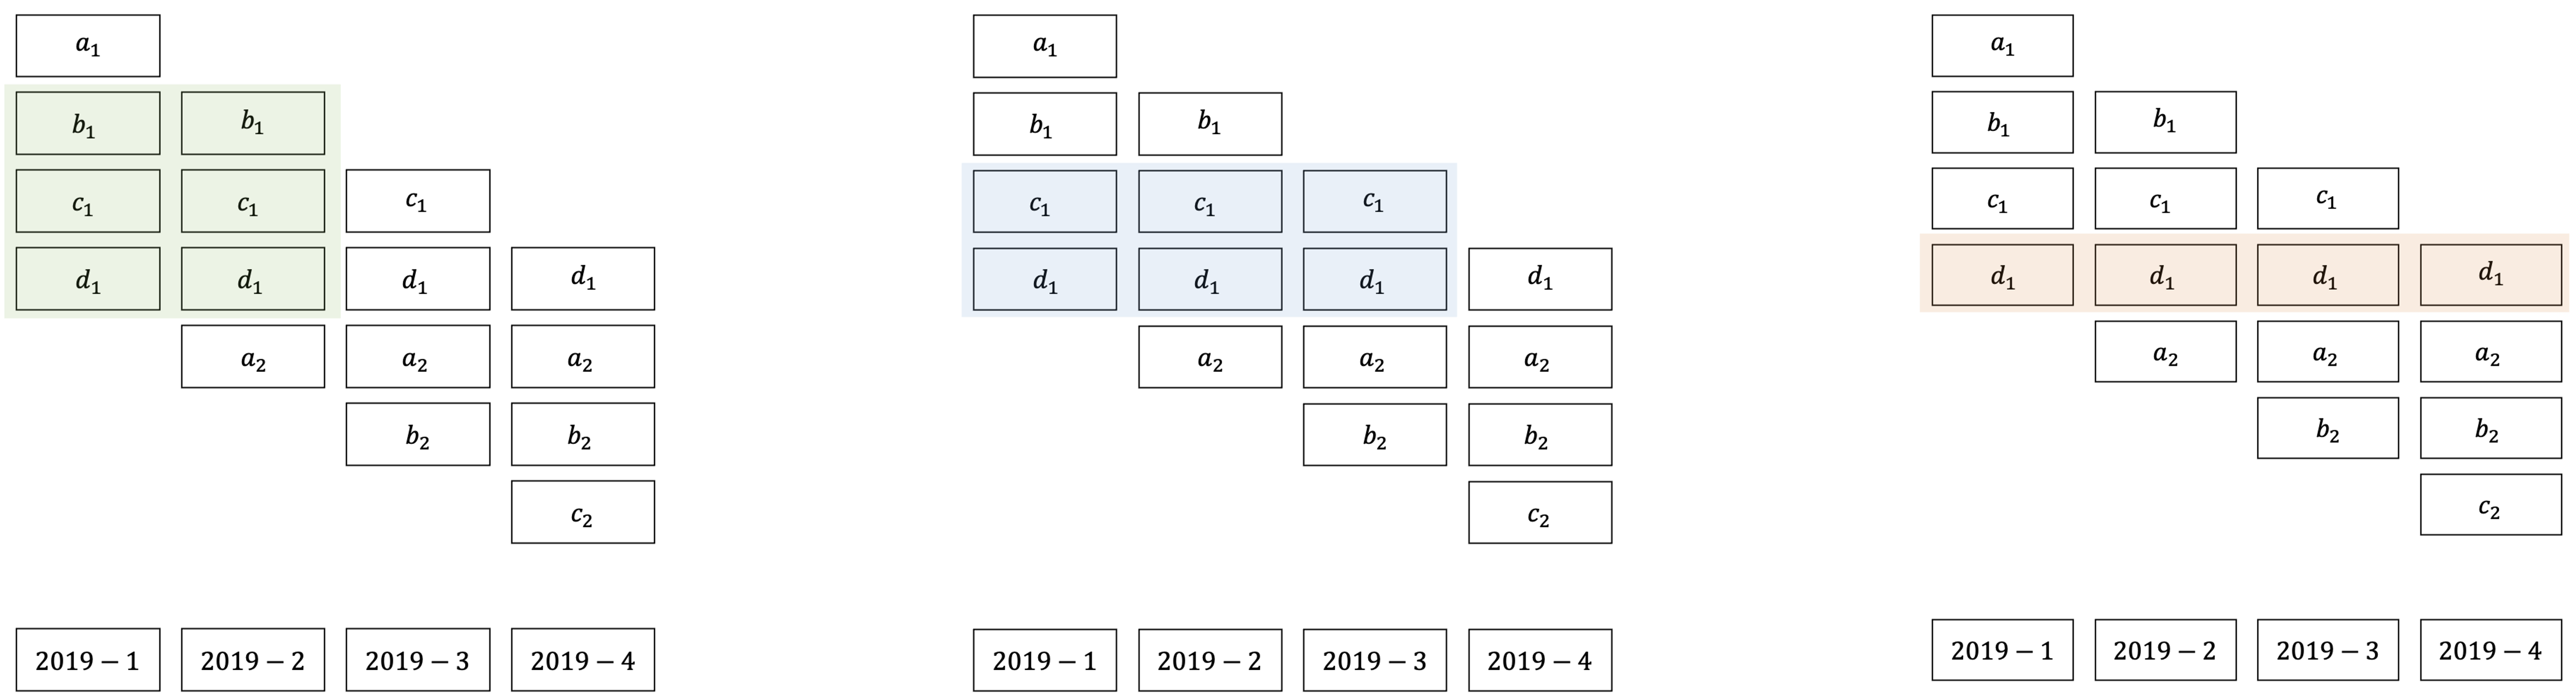
\includegraphics[width=0.5\linewidth]{Pics/el1} \caption{Tres escenarios longitudinales en un esquema rotativo 4(0)1.}\label{fig:figel1}
\end{figure}

Como se mencionó en capítulos anteriores, la pandemia por COVID-19 hizo que el año 2020 fuese un año atípico para los levantamientos de las encuestas de hogares en los INE de la región, puesto que la crisis de salud trajo consigo muchos retos en términos de la consecución de la información primaria. Debido a las restricciones de movilidad que los gobiernos tuvieron que imponer para hacerle frente a la pandemia, en algunos trimestres se optó por replicar el mismo esquema de trimestres anteriores. En nuestro ejemplo, asuma que no se incluyó el 25\% adicional que se tenía planeado, sino que la muestra fue exactamente la misma que en el primer trimestre. Recuérdese además que en casi toda la región, la muestra de hogares se contactó, no de manera presencial, sino telefónica, disminuyendo la tasa de cobertura y de respuesta efectiva.

\begin{longtable}[]{@{}cccccc@{}}
\caption{\emph{Rotación de páneles en el diseño 4(0)1 para 2020.}}\tabularnewline
\toprule()
Año & Trimestre & Panel 1 & Panel 2 & Panel 3 & Panel 4 \\
\midrule()
\endfirsthead
\toprule()
Año & Trimestre & Panel 1 & Panel 2 & Panel 3 & Panel 4 \\
\midrule()
\endhead
2020 & T1 & \(a_1\) & \(b_1\) & \(c_1\) & \(d_1\) \\
& T2 & \(b_1\) & \(c_1\) & \(d_1\) & \(a_2\) \\
& T3 & \(b_1\) & \(c_1\) & \(d_1\) & \(a_2\) \\
& T4 & \(c_1\) & \(d_1\) & \(a_2\) & \(b_2\) \\
\bottomrule()
\end{longtable}

En este ejemplo, el traslape de la muestra de hogares entre el segundo y el tercer trimestre de 2020 fue completo. Además, entre el primer y el tercer trimestre del 2020 hubo un 75\% de traslape; mientras que entre el primer trimestre y el último del 2020 hubo un 50\% de traslape.

\hypertarget{generaciuxf3n-de-bases-longitudinales-para-dos-periodos-consecutivos}{%
\section{Generación de bases longitudinales para dos periodos consecutivos}\label{generaciuxf3n-de-bases-longitudinales-para-dos-periodos-consecutivos}}

El análisis longitudinal de las encuestas de hogares es un insumo valioso en la toma de decisiones puesto que permite proveer una visión complementaria a los fenómenos sociales que no se puede obtener por otros medios. El seguimiento continuo a las unidades de observación no puede ser llevado a cabo en todas las encuestas continuas de la región, sino solamente en aquellas que contemplen esquemas rotativos en su planificación. Dado que en algunas encuestas, se contempla la asignación de la muestra a diferentes grupo de rotación, es posible analizar el comportamiento de los flujos brutos sobre indicadores tan importantes como los relacionados a la situación en la ocupación, la pobreza, entre otros.

En un contexto de estimación de cambios brutos con la definición de tablas de contingencia, \citet{Feinberg_Stasny_1983} asumen que las diferencias entre los pesos de muestreo en dos periodos de tiempo distintos ocurren solamente como resultado de los flujos naturales de entrada y
salida de la población de interés. Por ejemplo, si el individuo es
clasificado como empleado en ambos tiempos y \(w_k^{t-1}=300\) y
\(w_k^{t}=305\), entonces el peso mínimo, 300, se añade a la celda
(Empleado - Empleado) de la tabla de cambios brutos y la diferencia
entre los pesos, 5, se añade a la celda (Fuera - Empleado). Si por el
contrario, \(w_k^{t-1}=305\) y \(w_k^{t}=300\), entonces el peso mínimo,
300, se añade a la celda (Empleado - Empleado) de la tabla de cambios
brutos y la diferencia entre los pesos, 5, se añade a la celda (Empleado
- Fuera). Este enfoque supone que las diferencias entre los pesos están
supeditadas a las fluctuaciones que se puedan presentar en la fuerza de
trabajo.

El objetivo de esta sección es generar pesos longitudinales para todos los individuos pertenecientes a los paneles incumbentes de la muestra original en los dos primeros trimestre del 2020. Siguiendo la metodología de \citet{Verma_Betti_Ghellini}, es necesario seguir un procedimiento secuencial para la creación de los factores de expansión en el panel. En este orden de ideas, primero es necesario crear el conjunto de pesos iniciales (trasnversales en el primer periodo) para luego definir los pesos finales (longitudinales en el primer y segundo periodo). A continuación, se resume el procedimiento:

\begin{enumerate}
\def\labelenumi{\arabic{enumi}.}
\tightlist
\item
  Creación de pesos iniciales: teniendo en cuenta los pormenores del diseño de muestreo de la encuesta que selecciona una muestra de hogares y de personas que son miembros de estos hogares. Las ponderaciones iniciales se definen a partir de los factores de expansión transversales. Este proceso plantea al menos los siguientes pasos:

  \begin{itemize}
  \tightlist
  \item
    Determinación de los pesos básicos con el ajuste de selección de paneles rotativos.
  \item
    Ajuste por ausencia de respuesta y cobertura.
  \end{itemize}
\item
  Generación de los pesos longitudinales: la muestra debe ser modificada y ajustada para que refleje los cambios en la duración del panel para la población objetivo en los dos periodos de interés. En este caso se plantean al menos tres tipos de ajuste:

  \begin{itemize}
  \tightlist
  \item
    Definición de la población longitudinal (supeditada a los hogares que salen y entran en el periodo de referencia).
  \item
    Ausencia de respuesta y pérdidas en la muestra debido a la atrición (ausencia de respuesta en el panel).
  \item
    Calibración de los pesos longitudinales.
  \end{itemize}
\end{enumerate}

El primer paso en la generación de los pesos longitudinales consiste en realizar una consolidación (combinación) de bases de datos, en donde se integren únicamente los periodos de interés. Es decir que este proceso producirá bases de datos de diferentes tamaños para dos, tres o cuatro periodos. En general, se esperaría contar con un mayor número de unidades observacionales en el primer caso (dos periodos) y un número menor de unidades observacionales en el último caso (cuatro periodos). Nótese que en el caso particular del ejemplo (encuesta con un esquema rotativo 4(0)1), no es posible realizar la integración de cinco periodos consecutivos, puesto que el esquema solo define el traslape de hasta cuatro periodos consecutivos.

En general, es necesario asumir que al combinar los paneles y crear una sola base de datos, se está agregando información (puesto que se repiten las mediciones de los individuos pertenecientes a los paneles involucrados), pero al mismo tiempo se reduce el número de unidades observacionales (puesto que el número de individuos en la muestra que coinciden en los periodos de interés necesariamente es menor al número de individuos en la muestra de un corte transversal).

\hypertarget{creaciuxf3n-de-los-pesos-longitudinales-iniciales}{%
\subsection{Creación de los pesos longitudinales iniciales}\label{creaciuxf3n-de-los-pesos-longitudinales-iniciales}}

Este primer paso empieza con la definición de los periodos consecutivos que se utilizarán en la combinación de las bases de datos. Si la combinación se realiza para el año 2020, se debe tener en cuenta que hubo un cambio abrupto que se presentó como respuesta a las restricciones de movilidad que trajo la pandemia, que a su vez configuró un cambio en el modo de recolección (de presencial a telefónico) a partir del segundo trimestre del 2020.

Una vez definidos los periodos de interés, se debe realizar la combinación de las correspondientes bases de datos transversales. Este procedimiento debe tener en cuenta únicamente a las unidades muestrales que respondieron sistemáticamente en cada uno de los periodos de interés. En el escenario de la combinación de dos periodos, si una unidad respondió en ambos periodos será incluida en la base de datos combinada, de lo contrario (si respondió en el primer periodo, pero no en el segundo y viceversa) no será incluida en la base de datos.

\hypertarget{pesos-buxe1sicos}{%
\subsubsection{Pesos básicos}\label{pesos-buxe1sicos}}

La determinación de los pesos iniciales viene supeditada a los pesos básicos ajustados por cobertura \(d_{1, k}\) del procesamiento transversal del primer trimestre que se quiere combinar. Por ejemplo, el primer escenario de la figura anterior resalta que se quiere combinar el primer trimestre con el segundo trimestre del 2020; en este caso se partiría de los pesos básicos ajustados por cobertura del primer trimestre del 2020. En el segundo escenario se combinan el segundo y el tercer trimestre del 2020, por tanto se partiría de los pesos básicos ajustados por cobertura y ausencia de respuesta del segundo trimestre del 2020.

En general, dado que cada panel es representativo del país y, se supone que debe tener las mismas características al momento de la selección, \citet{LaRoche_2003} plantea que los pesos básicos se crean a partir del inverso de la probabilidad de inclusión de los paneles, así:

\[
d_{1, k}^{básico} = \frac{d_{1, k}}{Pr(\text{selección de paneles})}
\]

Al realizar la combinación de los dos primeros trimestres del 2020 en nuestro ejemplo es evidente que hay tres paneles coincidentes y como la muestra transversal contiene cuatro paneles, entonces \(Pr(\text{selección de paneles}) = \frac{3}{4}\). En cambio, por las condiciones asumidas para enfrentar la pandemia, cuando se realiza la combinación del segundo y tercer trimestre en el ejemplo se tiene que \(Pr(\text{selección de paneles}) = \frac{4}{4} = 1\).

Es importante notar que al combinar paneles, la inferencia que se realiza está supeditada al periodo del primer panel. Además, en este paso es indispensable corroborar que la suma de los pesos básicos esté cercana al tamaño de la población que se quiere representar. Es decir, \(\sum_{s^{(1)}} d_{1, k}^{básico} \approxeq N\); en donde \(s^{(1)}\) se define como el conjunto de respondientes en el primer periodo que pertenecen a los paneles coincidentes en la muestra para los periodos combinados.

De la misma forma, la metodología de la
encuesta \emph{Survey of Labour and Income Dynamics} \citep{Naud_2002, LaRoche_2003} plantea que un primer paso para crear los pesos longitudinales es mediante el ajuste por el inverso de la probabilidad de traslape).

\hypertarget{ajuste-por-ausencia-de-respuesta-1}{%
\subsubsection{Ajuste por ausencia de respuesta}\label{ajuste-por-ausencia-de-respuesta-1}}

A continuación, sobre los pesos básicos es necesario realizar un ajuste por ausencia de respuesta, que debería estar supeditado a las covariables disponibles en el marco de muestreo, en registros administrativos o, teniendo en cuenta el diseño de muestreo rotativo, en rondas anteriores de la misma encuesta. En general, es recomendable tener en cuenta el paradigma principal en el manejo de la ausencia de respuesta, el cual indica que respondientes y no respondientes difieren en la mayoría de los casos. Por supuesto, aquellas unidades que no respondieron deberán ser excluidas de la base de datos puesto que su peso de muestreo es nulo; es decir \(d_{1, k}^{básico} = 0, \ \forall k \notin s_r^{(1)}\), en donde el conjunto \(s_r^{(1)}\) representa a las unidades que respondieron la encuesta en el primer periodo de la combinación.

En este esquema, es posible utilizar un enfoque basado en la estimación de las probabilidades de respuesta de cada individuo para ajustar los pesos básicos, para lo cual se necesita establecer una relación entre las unidades que respondieron y que no respondieron con las covariables auxiliares \(\mathbf{x}_{1}\). En otras palabras, es necesario asegurar que las covariables estén disponibles para toda unidad seleccionada en el primer periodo de interés, independientemente de su respuesta final. Para el manejo efectivo de la ausencia de respuesta se consideran las variables dicotómicas \(I_{1, k}\) y \(D_{1, k}\), que indican si el hogar pertenece a la muestra del primer periodo y si respondió a la encuesta, respectivamente. La probabilidad de respuesta estará supeditada al siguiente modelo:

\[
\phi_{1, k} = Pr(D_{1, k} = 1|I_{1, k} = 1) = f(\mathbf{x}_{1}, \boldsymbol\beta)
\]

En la notación anterior, el conjunto de respondientes efectivos se define como aquel al que pertenecen las unidades muestrales que han respondido en el primer periodo de interés; además la función de enlace \(f\), es por lo general no lineal y su escogencia depende del investigador. Por otro lado, si se decide utilizar un modelo de regresión logística, entonces la estimación de las probabilidades de respuesta tendrá la siguiente forma:

\[
\hat{\phi}_{1, k} = \frac{\exp{(\mathbf{x}_{1}' \hat{\boldsymbol\beta})}}{1 +\exp{(\mathbf{x}_{1}' \hat{\boldsymbol\beta})}}
\]

Una vez que se ha modelado la ausencia de respuesta, los pesos básicos son ajustados utilizando el inverso de la probabilidad de respuesta sobre los respondientes efectivos en el primer periodo de interés, así se conforma el primer conjunto de pesos iniciales de las bases de datos longitudinales:

\[
d_{1, k}^{inicial} = \frac{d_{1, k}^{básico}}{\hat{\phi}_{1, k}}
\]

Es posible que, al construir la matriz de covariables para ajustar el modelo de respuesta, existan elementos que no respondieron en el primer periodo y que además no tengan información auxiliar porque su panel rotativo no se traslapa. En este caso, es posible calcular la tasa de respuesta efectiva y utilizarla como valor imputado a la probabilidad de respuesta \(\hat\phi_{1, k}\). También existen unidades que se acaban de incorporar al panel rotativo y por ende no respondieron y no tienen información auxiliar. En este caso, es necesario imputarles el factor de expansión ajustado del hogar al que pertenecen.

Como se mencionó en los capítulos anteriores, es necesario verificar las propiedades de balanceo y soporte común en el modelo de \emph{propensity score}. Se esperaría que la distribución de las probabilidades de respuesta para las combinaciones de los dos trimestres combinados mostraran un buen balance entre respondientes y no respondientes (distribuciones similares) y que el soporte común de la probabilidad de respuesta excluya al cero y al uno.

\hypertarget{creaciuxf3n-de-los-pesos-longitudinales-finales}{%
\subsection{Creación de los pesos longitudinales finales}\label{creaciuxf3n-de-los-pesos-longitudinales-finales}}

En este último paso, después de haber creado lo pesos longitudinales iniciales, se hacen algunos ajustes concernientes al periodo de combinación de las bases longitudinales, a la ausencia de respuesta entre estos periodos, y finalmente se realiza la calibración final para generar los pesos definitivos de la base de datos longitudinal.

\hypertarget{definiciuxf3n-de-la-poblaciuxf3n-longitudinal}{%
\subsubsection{Definición de la población longitudinal}\label{definiciuxf3n-de-la-poblaciuxf3n-longitudinal}}

La población longitudinal está supeditada a todas aquellas unidades que han permanecido en la población de interés entre el primer y el segundo periodo. Por ejemplo, en el caso de la encuesta que ejemplifica este capítulo, la población longitudinal del primer semestre del 2020 serían todas las personas que estuvieron en la población objetivo del primer periodo y que han permanecido en la población hasta el segundo periodo, inclusive.

Por supuesto, es necesario tener en cuenta que entre ambos periodos pueden haber ocurrido cambios en la población, como personas que han dejado de pertenecer a la población objetivo (por diversos motivos como la muerte, reclutamiento, internamiento en alguna institución, migración, entre otros). Siendo así, la población de interés en el segundo periodo sí contiene a las personas que han entrado (nacimientos, migración, licenciamiento de alguna institución, etc.) a conformar la población de interés desde el primer periodo, mientras que la población longitudinal no los contiene.

Es en esta segunda instancia en donde nacen los pesos definitivos y se construye la base longitudinal que será usada para realizar los análisis de interés. En primer lugar, se define la muestra longitudinal \(s^{(2)}\)como aquella constituida por las unidades seleccionadas en ambos periodos de interés para los paneles coincidentes; es decir, por la intersección de las muestras transversales del primer periodo \(s^1\) y el segundo periodo \(s^2\):

\[
s^{(2)} = s^1 \boldsymbol\cap s^2
\]

La muestra \(s^{(2)}\) es representativa de la población longitudinal en los dos periodos combinados. En esta etapa, el factor de expansión longitudinal se define como idéntico al peso resultante de la sección anterior; es decir \(d_{2, k}^{inicial} = d_{1, k}^{inicial}\).

\hypertarget{ausencia-de-respuesta-y-atriciuxf3n}{%
\subsubsection{Ausencia de respuesta y atrición}\label{ausencia-de-respuesta-y-atriciuxf3n}}

La conformación de la base de datos longitudinal parte de los pesos iniciales creados en la sección anterior. Sin embargo, hay que tener en cuenta que existirán unidades que no respondieron en alguno de los periodos de la combinación. En general, se forman tres subconjuntos de no respondientes; el primero conformado por las unidades que sí respondieron en el primer periodo y que no respondieron en el segundo, el segundo definido por las unidades que no respondieron en el primer periodo y que sí respondieron en el segundo, el tercero conformado por las unidades que no respondieron en ninguno de los periodos. En cualquiera de los anteriores casos es necesario identificar estas unidades a las cuales se le asignará un peso longitudinal nulo; es decir

\begin{equation*}
d_{2, k}^{inicial} =
\begin{cases}
d_{1, k}^{inicial}, &\ \forall k \in s_r^{(2)}  \\
0, &\ \forall k \notin s_r^{(2)}
\end{cases}
\end{equation*}

En donde el conjunto \(s_r^{(2)} = s_r^1 \boldsymbol\bigcap s_r^2\) representa a las unidades que respondieron la encuesta en ambos periodos de la combinación, es decir a todas las unidades respondientes en \(s^1\) que a la vez respondieron en \(s^2\). El raciocinio detrás de esta determinación es que, para todo efecto práctico de comparación entre periodos, los diseños de muestreo de las encuestas rotativas en la región inducen relativamente pocas combinaciones.

De la misma forma en que se realizó el ajuste en la sección anterior, es posible utilizar un enfoque basado en la estimación de las probabilidades de respuesta de cada individuo para ajustar los pesos iniciales, para lo cual se requiere de covariables auxiliares \(\mathbf{x}_{2}\) en el segundo periodo. Es así como se consideran las variables dicotómicas \(I_{2, k}\) y \(D_{2, k}\), que indican si la unidad pertenece a la muestra del segundo periodo y si respondió a la encuesta en el segundo periodo, respectivamente. La probabilidad de respuesta estará supeditada al siguiente modelo:

\[
\phi_{2, k} = Pr(D_{2, k} = 1|I_{2, k} = 1) = f(\mathbf{x}_{2}, \boldsymbol\beta)
\]

Una vez que se ha modelado la ausencia de respuesta, los pesos longitudinales son ajustados utilizando el inverso de la probabilidad de respuesta sobre los respondientes efectivos en el primer periodo de interés:

\[
d_{2, k}^{longitudinal} = \frac{d_{2, k}^{inicial}}{\hat{\phi}_{2, k} }
\]

\hypertarget{calibraciuxf3n-de-los-pesos-longitudinales}{%
\subsubsection{Calibración de los pesos longitudinales}\label{calibraciuxf3n-de-los-pesos-longitudinales}}

Luego del ajuste por ausencia de respuesta es aconsejable imponer algunas restricciones sobre los factores de expansión; en particular, se busca que la suma de los pesos reproduzca con exactitud los conteos poblacionales, o las proyecciones demográficas, en el país, en las regiones o departamentos, en los subgrupos de edad y sexo, en las áreas urbana y rural, etc. En general, en las restricciones de la calibración pueden intervenir tanto variables a nivel de individuo como de hogar. Es importante enfatizar que los totales auxiliares usados en la calibración deben representar la población del primer periodo de interés, puesto que, al conformar un panel que no adiciona elementos a lo largo de los periodos de medición, la muestra será representativa únicamente del periodo en cual fue seleccionada. Teniendo en cuenta que las variables de calibración están representadas por el vector \(\mathbf{z}_k\) y que sus totales poblacionales están disponibles en forma de proyecciones poblacionales, entonces este conjunto de restricciones sobre los nuevos pesos longitudinales calibrados \(w_{2, k}^{calibrado}\) se puede escribir como:

\[
\sum_{s_r^{(2)}} w_{2, k}^{calibrado} \  \mathbf{z}_k = \sum_{U} \mathbf{z}_k
\]

Por lo tanto, los pesos finales que deberían incluirse en la base de datos longitudinal de los dos trimestres combinados, estarían dados por \(w_{2, k}^{calibrado}\), los cuales pueden escribirse como sigue:

\[
w_{2, k}^{calibrado} = g_k * d_{2, k}^{longitudinal}
\]

En donde los ponderadores \(g_k\) dependen de la muestra traslapada y representan la cercanía de los pesos finales longitudinales calibrados con los pesos longitudinales sin calibrar. Se esperaría que estos valores estuvieran cercanos, en general, a la unidad.

\hypertarget{generaciuxf3n-de-bases-longitudinales-anuales}{%
\section{Generación de bases longitudinales anuales}\label{generaciuxf3n-de-bases-longitudinales-anuales}}

En esta sección se describen los pasos necesarios para combinar bases de datos longitudinales que permitan hacer seguimiento a la situación de los hogares a lo largo de todo un año. La metodología que se recomienda implementar es una generalización de los pasos descritos en \citet{Verma_Betti_Ghellini}, que define un procedimiento secuencial para la creación de los factores de expansión en el panel. El raciocinio de este procedimiento sigue exactamente los mismos pasos que los mencionados anteriormente en la creación de bases longitudinales para dos periodos consecutivos. Es decir, primero es necesario crear el conjunto de pesos iniciales (transversales en el primer periodo) para luego definir los pesos finales (longitudinales en los cuatro trimestres de todo un año).

El primer paso en la generación de los pesos longitudinales consiste en realizar una consolidación de bases de datos, en donde se combinen únicamente los periodos de interés. Siguiendo con el ejemplo del esquema 4(0)1, correspondería a los cuatro trimestres del año. Para esto, es necesario filtrar cada una de las bases transversales con el identificador del panel de interés. De esta forma se tendrán cuatro bases de datos conteniendo únicamente la información de estos paneles comunes.

La determinación de los pesos iniciales viene supeditada a los pesos básicos ajustados por cobertura \(d_{(1,k)}\) del procesamiento transversal del primer trimestre que se quiere combinar. En general, los pesos básicos se crean a partir del inverso de la probabilidad de inclusión de los paneles; puesto que, al realizar la combinación de los cuatro trimestres en un esquema 4(0)1, es evidente que hay un solo panel coincidente y como la muestra transversal contiene cuatro paneles, entonces \(Pr(\text{selección de paneles}) = 1/4\). En resumen,

\[
d_{(1,k)}^{básico}= \dfrac{d_{(1,k)}}{Pr(\text{selección de paneles})} = 4 \times d_{(1,k)} 
\]

Como se anotó anteriormente, se debe seguir un proceso riguroso de identificación secuencial de respondientes y no respondientes para poder realizar la combinación de las correspondientes bases de datos transversales. Este procedimiento debe tener en cuenta únicamente a las unidades muestrales que respondieron sistemáticamente en cada uno de los periodos de interés. Por lo tanto se sugiere que se sigan los siguientes pasos:

\begin{enumerate}
\def\labelenumi{\arabic{enumi}.}
\tightlist
\item
  Trimestre T1 y T2.

  \begin{itemize}
  \tightlist
  \item
    Identificación de los respondientes en T1 y T2.
  \item
    Identificación de quienes respondieron en T1 pero no en T2.
  \end{itemize}
\item
  Trimestre T1, T2 y T3.

  \begin{itemize}
  \tightlist
  \item
    Identificación de los respondientes en T1, T2 y T3.
  \item
    Identificación de quienes respondieron en T1 y en T2, pero no en T3.
  \end{itemize}
\item
  Trimestre T1, T2, T3 y T4.

  \begin{itemize}
  \tightlist
  \item
    Identificación de los respondientes en T1, T2, T3 y T4.
  \item
    Identificación de quienes respondieron en T1, T2 y en T3, pero no en T4.
  \end{itemize}
\end{enumerate}

En esta instancia se construye la base longitudinal que será usada para realizar los análisis de interés. En primer lugar, se define la muestra longitudinal \(s^{(1234)}\) como aquella constituida por las unidades seleccionadas en ambos periodos de interés para los paneles coincidentes:
\[
s^{(1234)}=s^1 \cap s^2 \cap s^3 \cap s^4
\]

La muestra \(s^{(1234)}\) es representativa de la población longitudinal en los periodos combinados. En esta etapa, el factor de expansión longitudinal inicial se define como idéntico al peso resultante de la sección anterior; es decir

\[
d_{(1234,k)}^{inicial}=d_{(1,k)}^{inicial}
\]

Es necesario identificar las unidades que no respondieron en alguna ocasión para asignarles un peso longitudinal nulo; es decir
\(d_{(1234,k)}^{inicial}=0\) para aquellas unidades \(k \notin s_r^{(1234)}\); en donde el conjunto \(s_r^{(1234)}\) representa a las unidades que respondieron la encuesta en todos los cuatro trimestres de la combinación. Sin embargo, estas unidades que no respondieron en alguna ocasión se utilizarán para ajustar el modelo de \emph{propensity score}, antes de que sean excluidas totalmente de la base de datos (puesto que su peso de muestreo es nulo).

Con base en la identificación de respondientes y no respondientes a lo largo del año, el siguiente paso necesario es realizar el ajuste por ausencia de respuesta, que debería estar supeditado a las covariables disponibles en el marco de muestreo, o en rondas anteriores de la misma encuesta. Como se ha indicado a lo largo de este documento, se recomienda usar un enfoque basado en la estimación de las propensiones de respuesta de cada individuo para ajustar los pesos básicos. La probabilidad de respuesta estará supeditada al siguiente modelo:

\[
\phi_{(1234,k)}=Pr(D_{(1234,k)}=1|I_{(1234,k)}=1)=f(x,\beta)
\]

En la notación anterior, el conjunto de respondientes efectivos se define como aquel al que pertenecen las unidades muestrales que han respondido en todos los periodos de interés. Los pesos básicos son ajustados utilizando el inverso de la probabilidad estimada de respuesta sobre los respondientes efectivos en el primer periodo de interés, así se conforma el primer conjunto de pesos iniciales de las bases de datos longitudinales. Por último, se debe corroborar que la suma de los pesos ajustados por la ausencia de respuesta esté cercana al tamaño de la población que se quiere representar.

Luego del ajuste por ausencia de respuesta, el proceso termina con la calibración final; en donde se imponen algunas restricciones sobre los factores de expansión finales; en particular, se busca que la suma de los pesos reproduzca con exactitud los conteos poblacionales, o las proyecciones demográficas.

Una observación pertinente que debe realizarse es que la base de datos longitudinal representa con exactitud al conjunto de individuos comunes en los periodos de interés; por consiguiente, las estimaciones transversales que se hagan a partir de esta base (por ejemplo, pobreza en un determinado trimestre, entre otras) solo deben tomarse de manera referencial, puesto que no reemplazarán a las estimaciones transversales ya publicadas. Nótese que la población de interés de la encuesta transversal no es la misma que la de la combinación (panel) y por ende, estas estimaciones no coincidirán y no debieran coincidir.

La razón de la creación de las bases de datos longitudinales reside grandemente en la estimación de los flujos brutos, su error de muestreo asociado y sus correspondientes intervalos de confianza. La ganancia en el análisis es muy grande cuando se conocen las estimaciones entre estados de una variable de interés. Por ejemplo, los usuarios de la encuesta pueden estar interesados en analizar el cambio bruto (flujos) entre diferentes estados de la fuerza de trabajo; es decir, aquellos que estaban ocupados en un trimestre T1 cómo se encuentran en el siguiente trimestre T2. Este tipo de análisis se traduce comúnmente en la estimación de matrices de transición, que serán tratadas en el siguiente capítulo.

\hypertarget{anuxe1lisis-de-flujos-brutos}{%
\chapter{Análisis de flujos brutos}\label{anuxe1lisis-de-flujos-brutos}}

Existen ventajas marcadas a la hora de analizar datos que provienen de levantamientos longitudinales. \citet{Lynn_2009} menciona que la más común de ellas es la posibilidad de realizar análisis de los fujos brutos. Con los levantamientos longitudinales es posible establecer el estado de una unidad observacional en varios periodos consecutivos. Esto permite descomponer los cambios netos que uno podría encontrar en las encuestas transversales. Por ejemplo, a partir de los levantamientos transversales (puntuales en un trimestre), en una encuesta con diseño rotativo es posible estimar el cambio en las diferentes clasificaciones del mercado de trabajo, de un periodo a otro. En efecto, usando la parte longitudinal de la encuesta en ambos periodos, es posible descomponer estas clasificaciones. A partir de este análisis es posible identificar si son exactamente los mismos ocupados los que entran al mercado de trabajo en dos ciclos económicos de interés.

Un problema común que se encuentra en este tipo de encuesta es la ausencia de respuesta, que rara vez se puede considerar como aleatoria o ignorable. Si la ausencia de respuesta depende del estado ocupacional (por ejemplo, las tasas de ausencia de respuesta son más altas entre los desempleados), las estimaciones ingenuas de los cambios brutos podrían estar sesgadas. Si el enfoque corrige la ausencia de respuesta pero ignora las complejas características del diseño de muestreo, también habrá problemas de sesgo.

\hypertarget{matrices-de-transiciuxf3n}{%
\section{Matrices de transición}\label{matrices-de-transiciuxf3n}}

La inferencia realizada en la estimación de parámetros mediante encuestas de hogares recae en el diseño de muestreo que se utilizó para seleccionar una muestra de elementos de la población. Por lo general, en términos de la obtención de estadísticas oficiales, el diseño de muestreo utilizado no es simple, puesto que, por la complejidad de la estructura poblacional, es necesario recurrir a técnicas especializadas, que permiten la apropiada consecución de la información en la muestra. En muchas ocasiones, el diseño de muestreo complejo de las encuestas de hogares está supeditado a la estratificación de las unidades cartográficas del marco de muestreo, y a la posterior selección multietápica de unidades de muestreo, usualmente con probabilidades de inclusión desiguales y proporcionales al número de habitantes de las áreas en las que se divide el marco de muestreo.

Después de haber seleccionado una muestra probabilística, es común recurrir a la clasificación de los elementos de la población en diferentes categorías de una o más variables nominales. Dicha clasificación se puede convertir en una tabla de contingencias si se resumen simultáneamente dos variables o, los cambios en el comportamiento de una misma variable en dos periodos de tiempo. Este es el caso de la estimación de los cambios brutos entre diferentes estados de clasificación para dos periodos. En particular, este problema de estimación es fundamental para la implementación de políticas públicas en el mercado laboral.

Como ya se ha discutido a profundidad, muchas encuestas por muestreo a gran escala en la región utilizan diseños del tipo panel rotativo donde los individuos son entrevistados varias veces antes de ser rotados y excluidos fuera de la muestra. Estas encuestas a gran escala son utilizadas para producir estimaciones puntuales en el tiempo de manera continua, mensual y trimestral. Además, su estructura de seguimiento en panel nace de la necesidad de mantener una estructura suavizada en los cambios coyunturales del fenómeno de interés, además de poder reducir costos manteniendo los mismos entrevistados y objetivos por más de una entrevista.

Debido a los efectos de la pandemia de COVID-19 y en particular a las diferentes restricciones de movilidad que se promovieron desde los gobiernos de los países de la región (cuarentenas obligatorias y toques de queda), la forma de recolectar la información en las encuestas de hogares tuvo que ser modificada y se cambiaron abruptamente los levantamientos presenciales por levantamientos telefónicos que indujeron tasas de respuesta bajas que eventualmente indujeron nuevos procesos estadísticos en el ajuste de los factores de expansión con el fin de identificar y eliminar lo posibles sesgos potenciales que pudieron introducirse.

Por ende, es natural contemplar la posibilidad de que para estos tipos de levantamientos la ausencia de respuesta no necesariamente sea completamente aleatoria. De hecho, muy probablemente, la ausencia de respuesta podría depender del estado de clasificación en la ocupación (por ejemplo, que los desempleados conformen la mayoría de no respondientes), y que las estimaciones de los cambios brutos deban contemplar correcciones ante posibles sesgos.

\hypertarget{modelos-de-markov}{%
\section{Modelos de Markov}\label{modelos-de-markov}}

Al considerar el problema de la estimación de los cambios brutos entre dos periodos de tiempo, obtenidos de una investigación sobre la población de interés, y teniendo en cuenta que existe ausencia de respuesta no ignorable, es posible suponer que el resultado de cada entrevista corresponde a la clasificación del respondiente en una de \(G\) posibles categorías excluyentes. Por ende, uno de los objetivos de la investigación podría ser la estimación del cambio bruto entre estas categorías utilizando la información de los individuos que fueron entrevistados en dos periodos de tiempo consecutivos. La siguiente tabla ejemplifica la distribución (no observable) de los flujos brutos en una población.

\begin{longtable}[]{@{}
  >{\raggedright\arraybackslash}p{(\columnwidth - 12\tabcolsep) * \real{0.1429}}
  >{\raggedright\arraybackslash}p{(\columnwidth - 12\tabcolsep) * \real{0.1429}}
  >{\raggedright\arraybackslash}p{(\columnwidth - 12\tabcolsep) * \real{0.1429}}
  >{\raggedright\arraybackslash}p{(\columnwidth - 12\tabcolsep) * \real{0.1429}}
  >{\raggedright\arraybackslash}p{(\columnwidth - 12\tabcolsep) * \real{0.1429}}
  >{\raggedright\arraybackslash}p{(\columnwidth - 12\tabcolsep) * \real{0.1429}}
  >{\raggedright\arraybackslash}p{(\columnwidth - 12\tabcolsep) * \real{0.1429}}@{}}
\caption{Distribución no observable de los flujos brutos en una población.}\tabularnewline
\toprule()
\begin{minipage}[b]{\linewidth}\raggedright
Estado (T1/T2)
\end{minipage} & \begin{minipage}[b]{\linewidth}\raggedright
1
\end{minipage} & \begin{minipage}[b]{\linewidth}\raggedright
2
\end{minipage} & \begin{minipage}[b]{\linewidth}\raggedright
\(\cdots\)
\end{minipage} & \begin{minipage}[b]{\linewidth}\raggedright
j
\end{minipage} & \begin{minipage}[b]{\linewidth}\raggedright
\(\cdots\)
\end{minipage} & \begin{minipage}[b]{\linewidth}\raggedright
G
\end{minipage} \\
\midrule()
\endfirsthead
\toprule()
\begin{minipage}[b]{\linewidth}\raggedright
Estado (T1/T2)
\end{minipage} & \begin{minipage}[b]{\linewidth}\raggedright
1
\end{minipage} & \begin{minipage}[b]{\linewidth}\raggedright
2
\end{minipage} & \begin{minipage}[b]{\linewidth}\raggedright
\(\cdots\)
\end{minipage} & \begin{minipage}[b]{\linewidth}\raggedright
j
\end{minipage} & \begin{minipage}[b]{\linewidth}\raggedright
\(\cdots\)
\end{minipage} & \begin{minipage}[b]{\linewidth}\raggedright
G
\end{minipage} \\
\midrule()
\endhead
1 & \(X_{11}\) & \(X_{12}\) & \(\cdots\) & \(X_{1j}\) & \(\cdots\) & \(X_{1G}\) \\
2 & \(X_{21}\) & \(X_{22}\) & \(\cdots\) & \(X_{2j}\) & \(\cdots\) & \(X_{2G}\) \\
\(\vdots\) & \(\vdots\) & \(\vdots\) & \(\ddots\) & \(\vdots\) & \(\ddots\) & \(\vdots\) \\
i & \(X_{i1}\) & \(X_{i2}\) & \(\cdots\) & \(X_{ij}\) & \(\cdots\) & \(X_{iG}\) \\
\(\vdots\) & \(\vdots\) & \(\vdots\) & \(\ddots\) & \(\vdots\) & \(\ddots\) & \(\vdots\) \\
G & \(X_{G1}\) & \(X_{G2}\) & \(\cdots\) & \(X_{Gj}\) & \(\cdots\) & \(X_{GG}\) \\
\bottomrule()
\end{longtable}

En donde \(X_{ij}\) es el número de unidades en la población finita clasificadas como \(i\) en el tiempo \(t-1\) y \(j\) en el tiempo \(t\) (\(i,j=1,\ldots, G\)). Siguiendo las consideraciones de \citet{Feinberg_Stasny_1983} se asume que los datos son el resultado de un proceso de dos etapas. En la primera etapa (proceso no observable), los individuos son ubicados dentro de las celdas de una matriz \(G\times G\) de acuerdo con las probabilidades de una cadena de Markov, con los siguientes parámetros:

\begin{enumerate}
\def\labelenumi{\arabic{enumi}.}
\tightlist
\item
  \(\eta_i\), la probabilidad inicial de que un individuo esté en el estado \(i\) en el tiempo \(t-1\).
\item
  \(p_{ij}\), la probabilidad de transición desde el estado \(i\) al estado \(j\).
\end{enumerate}

Nótese que en esta primera etapa los parámetros deben cumplir con las siguientes restricciones: \(\sum_i\eta_i=1\) y \(\sum_jp_{ij}=1\) para todo \(i\).

Es claro que, una vez se realice la encuesta y se obtengan los datos de los levantamientos en ambos periodos, los individuos que fueron no respondientes en uno o ambos periodos o fueron incluidos o excluidos de la muestra entre estos dos tiempos no tienen una clasificación definida entre las categorías. De esta forma, se tiene un grupo de individuos con clasificación en ambos tiempos, un grupo de individuos que solo tiene clasificación en uno de los dos tiempos, y un grupo de individuos que no respondieron la encuesta en ningún periodo de tiempo, y por ende nunca fueron clasificados.

Para el primer grupo de individuos que respondieron en los tiempos \(t-1\) y \(t\), los datos de clasificación pueden ser resumidos en una matriz de tamaño \(G\times G\). La información disponible para los individuos que fueron no respondientes para la encuesta del tiempo \(t-1\), pero sí respondieron en el tiempo \(t\), puede ser resumida en un complemento columna; mientras que la información para los individuos que no respondieron en el tiempo \(t\), pero sí respondieron en el tiempo \(t-1\), puede ser resumida en un complemento fila. Finalmente, los individuos que no respondieron en ningún tiempo son incluidos en una única celda de faltantes.

Las anteriores relaciones se ilustran en la siguiente tabla, en donde \(N_{ij}\) (\(i,j=1,\ldots,G\); \(G=4\)) denota el número de individuos respondientes que tienen clasificación \(i\) en el tiempo \(t-1\) y \(j\) en el tiempo \(t\), \(R_i\) denota el número de individuos que fueron no respondientes en el tiempo \(t\) y tienen clasificación \(i\) en el tiempo \(t-1\), \(C_j\) denota el número de individuos que fueron no respondientes en el tiempo \(t-1\) y tuvieron clasificación \(j\) en el tiempo \(t\), y \(M\) denota el número de individuos seleccionados que no respondieron en ningún tiempo. En este estudio particular se consideran cuatro estados de clasificación (ocupados formales, ocupados informales, desocupados, inactivos) - por ende \(G = 4\) - en dos periodos consecutivos de tiempo \(t-1\), primer trimestre del 2020 y \(t\), segundo trimestre del 2020.

\begin{longtable}[]{@{}
  >{\raggedright\arraybackslash}p{(\columnwidth - 10\tabcolsep) * \real{0.2593}}
  >{\raggedright\arraybackslash}p{(\columnwidth - 10\tabcolsep) * \real{0.1235}}
  >{\raggedright\arraybackslash}p{(\columnwidth - 10\tabcolsep) * \real{0.1235}}
  >{\raggedright\arraybackslash}p{(\columnwidth - 10\tabcolsep) * \real{0.1481}}
  >{\raggedright\arraybackslash}p{(\columnwidth - 10\tabcolsep) * \real{0.1235}}
  >{\raggedright\arraybackslash}p{(\columnwidth - 10\tabcolsep) * \real{0.2222}}@{}}
\caption{Distribución observable de los flujos brutos en la población con ausencia de respuesta en ambos periodos.}\tabularnewline
\toprule()
\begin{minipage}[b]{\linewidth}\raggedright
Estado (T1/T2)
\end{minipage} & \begin{minipage}[b]{\linewidth}\raggedright
Formal
\end{minipage} & \begin{minipage}[b]{\linewidth}\raggedright
Informal
\end{minipage} & \begin{minipage}[b]{\linewidth}\raggedright
Desocupado
\end{minipage} & \begin{minipage}[b]{\linewidth}\raggedright
Inactivo
\end{minipage} & \begin{minipage}[b]{\linewidth}\raggedright
Complemento fila
\end{minipage} \\
\midrule()
\endfirsthead
\toprule()
\begin{minipage}[b]{\linewidth}\raggedright
Estado (T1/T2)
\end{minipage} & \begin{minipage}[b]{\linewidth}\raggedright
Formal
\end{minipage} & \begin{minipage}[b]{\linewidth}\raggedright
Informal
\end{minipage} & \begin{minipage}[b]{\linewidth}\raggedright
Desocupado
\end{minipage} & \begin{minipage}[b]{\linewidth}\raggedright
Inactivo
\end{minipage} & \begin{minipage}[b]{\linewidth}\raggedright
Complemento fila
\end{minipage} \\
\midrule()
\endhead
Formal & \(N_{11}\) & \(N_{12}\) & \(N_{13}\) & \(N_{14}\) & \(R_1\) \\
Informal & \(N_{21}\) & \(N_{22}\) & \(N_{23}\) & \(N_{24}\) & \(R_2\) \\
Desocupado & \(N_{31}\) & \(N_{32}\) & \(N_{33}\) & \(N_{34}\) & \(R_3\) \\
Inactivo & \(N_{41}\) & \(N_{42}\) & \(N_{43}\) & \(N_{44}\) & \(R_4\) \\
Complemento columna & \(C_1\) & \(C_2\) & \(C_3\) & \(C_4\) & \(M\) \\
\bottomrule()
\end{longtable}

En la segunda etapa (proceso observable), cada individuo en la celda \(ij\) de la matriz puede ser no respondiente en el tiempo \(t-1\) y perder la clasificación por fila, o ser no respondiente en el tiempo \(t\) y perder la clasificación columna, o bien, ser no respondiente en ambos tiempos y perder ambas clasificaciones. Por ende, se genera una estructura probabilística con los siguientes parámetros:

\begin{enumerate}
\def\labelenumi{\arabic{enumi}.}
\tightlist
\item
  \(\psi(i,j)\), la probabilidad inicial de que un individuo en la celda \(ij\) responda en el tiempo \(t-1\).
\item
  \(\rho_{RR}(i,j)\), la probabilidad de transición de que un individuo en la celda \(ij\) pase de ser respondiente en el tiempo \(t-1\) a ser respondiente en el tiempo \(t\).
\item
  \(\rho_{MM}(i,j)\), la probabilidad de transición de que un individuo en la celda \(ij\) pase de ser no respondiente en el tiempo \(t-1\) a ser no respondiente en el tiempo \(t\).
\end{enumerate}

Como se puede notar las probabilidades del proceso observables dependen del estado de clasificación del individuo. Para estimar todos los parámetros involucrados, se consideraron los siguientes modelos reducidos, explicados a continuación:

\begin{itemize}
\tightlist
\item
  Modelo A: considera que la probabilidad inicial de que un individuo sea respondiente en el tiempo \(t-1\) es la misma para todas las clasificaciones contempladas en la encuesta, es decir \(\psi(i,j)=\psi\). Las probabilidades de transición entre respondientes y entre no respondientes no dependen de la clasificación del individuo en la encuesta, es decir \(\rho_{MM}(i,j)=\rho_{MM}\) y \(\rho_{RR}(i,j)=\rho_{RR}\). Es decir que la probabilidad de tránsito entre respondientes es la misma para formales, informales, inactivos y desocupados; asimismo las probabilidades de respuesta se consideran idénticas para las diferentes clasificaciones.
\item
  Modelo B: considera que la probabilidad inicial de que un individuo sea respondiente en el tiempo \(t-1\) depende de su clasificación en el tiempo \(t-1\), es decir \(\psi(i,j)=\psi(i)\). De la misma manera que en el modelo A, las probabilidades de transición entre respondientes y entre no respondientes no dependerán de la clasificación del individuo en la encuesta, es decir \(\rho_{MM}(i,j)=\rho_{MM}\) y \(\rho_{RR}(i,j)=\rho_{RR}\). Es decir que la probabilidad de respuesta difiere entre formales, informales, inactivos e desocupados; mientras que la probabilidad de tránsito entre respondientes es la misma.
\item
  Modelo C: asume que la probabilidad inicial de que un individuo sea respondiente en el tiempo \(t-1\) es la misma para todas las clasificaciones contempladas en la encuesta, es decir \(\psi(i,j)=\psi\). Sin embargo, las probabilidades de transición entre respondientes y entre no respondientes dependerán de la clasificación del individuo en el periodo \(t-1\); es decir \(\rho_{MM}(i,j)=\rho_{MM}(i)\) y \(\rho_{RR}(i,j)=\rho_{RR}(i)\). Es decir que la probabilidad de tránsito entre respondientes es la misma para formales, informales, inactivos e desocupados; asimismo las probabilidades de transición difieren para las diferentes clasificaciones en el tiempo inicial.
\item
  Modelo D: asume que la probabilidad inicial de que un individuo sea respondiente en el tiempo \(t-1\) es la misma para todas las clasificaciones contempladas en la encuesta, es decir \(\psi(i,j)=\psi\). Sin embargo, las probabilidades de transición entre respondientes y entre no respondientes dependerán de la clasificación del individuo en el periodo \(t\); es decir \(\rho_{MM}(i,j)=\rho_{MM}(j)\) y \(\rho_{RR}(i,j)=\rho_{RR}(j)\). Es decir que la probabilidad de respuesta es la misma para formales, informales, inactivos e desocupados; asimismo la probabilidad de tránsito entre respondientes difiere para las diferentes clasificaciones en el tiempo final.
\end{itemize}

Ampliando las ideas de \citet{Feinberg_Stasny_1983}, \citet{Gutierrez_2014} consideró una metodología de estimación basada en el enfoque de máxima-pseudo verosimilitud para estimar lo anteriores parámetros. El objetivo final del proceso es estimar el número de individuos en las celdas de una tabla de contingencia poblacional donde se clasifican según la situación de la fuerza laboral medida en dos puntos de tiempo diferentes bajo un diseño de muestreo complejo. En resumen, el ajuste de los modelos de ausencia de respuesta puede ser realizado siguiendo los algoritmos de estimación propuestos en \citet{Gutierrez_2014}, y utilizando el paquete computacional \texttt{surf} implementado en el software estadístico \texttt{R} \citep{Jacob_2020}.

\hypertarget{estimaciuxf3n-de-las-matrices-de-transiciuxf3n}{%
\section{Estimación de las matrices de transición}\label{estimaciuxf3n-de-las-matrices-de-transiciuxf3n}}

Considere que se dispone de información sobre la situación laboral de 41274 personas para los dos primeros trimestres del 2020 (año en el que la pandemia por COVID-19 produjo alteraciones importantes en el levantamiento regular de las encuestas y en el mercado de trabajo). La clasificación del estatus ocupacional en la muestra se da en la siguiente tabla; la cual contiene los complementos columna y los complementos fila para las personas que no respondieron en alguno de los dos períodos. Nótese que los valores del complemento fila son mucho mayores que el complemento columna, lo que puede ser causado por la pandemia. Nótese que la suma de todas las entradas de la tabla de clasificación da como resultado el número de personas en la muestra traslapada, es decir 41,274 individuos.

\begin{longtable}[]{@{}
  >{\raggedright\arraybackslash}p{(\columnwidth - 10\tabcolsep) * \real{0.2658}}
  >{\raggedright\arraybackslash}p{(\columnwidth - 10\tabcolsep) * \real{0.1013}}
  >{\raggedright\arraybackslash}p{(\columnwidth - 10\tabcolsep) * \real{0.1266}}
  >{\raggedright\arraybackslash}p{(\columnwidth - 10\tabcolsep) * \real{0.1519}}
  >{\raggedright\arraybackslash}p{(\columnwidth - 10\tabcolsep) * \real{0.1266}}
  >{\raggedright\arraybackslash}p{(\columnwidth - 10\tabcolsep) * \real{0.2278}}@{}}
\caption{Distribución observada de los flujos brutos en la muestra no ponderada con ausencia de respuesta en ambos periodos.}\tabularnewline
\toprule()
\begin{minipage}[b]{\linewidth}\raggedright
Estado (T1/T2)
\end{minipage} & \begin{minipage}[b]{\linewidth}\raggedright
Formal
\end{minipage} & \begin{minipage}[b]{\linewidth}\raggedright
Informal
\end{minipage} & \begin{minipage}[b]{\linewidth}\raggedright
Desocupado
\end{minipage} & \begin{minipage}[b]{\linewidth}\raggedright
Inactivo
\end{minipage} & \begin{minipage}[b]{\linewidth}\raggedright
Complemento fila
\end{minipage} \\
\midrule()
\endfirsthead
\toprule()
\begin{minipage}[b]{\linewidth}\raggedright
Estado (T1/T2)
\end{minipage} & \begin{minipage}[b]{\linewidth}\raggedright
Formal
\end{minipage} & \begin{minipage}[b]{\linewidth}\raggedright
Informal
\end{minipage} & \begin{minipage}[b]{\linewidth}\raggedright
Desocupado
\end{minipage} & \begin{minipage}[b]{\linewidth}\raggedright
Inactivo
\end{minipage} & \begin{minipage}[b]{\linewidth}\raggedright
Complemento fila
\end{minipage} \\
\midrule()
\endhead
Formal & 11483 & 718 & 592 & 1828 & 451 \\
Informal & 703 & 2513 & 495 & 2769 & 198 \\
Desocupado & 191 & 181 & 503 & 794 & 81 \\
Inactivo & 364 & 641 & 388 & 15386 & 382 \\
Complemento columna & 160 & 65 & 48 & 257 & 83 \\
\bottomrule()
\end{longtable}

Como se supone que la muestra proviene de un muestreo complejo sobre la población del país, para utilizar el método de estimación propuesto en esta sección, se necesita primero estimar el tamaño de la población en cada celda de la tabla anterior. Estas estimaciones se dan en la siguiente tabla donde el tamaño de población estimado es 15,597,572.

\begin{longtable}[]{@{}
  >{\raggedright\arraybackslash}p{(\columnwidth - 10\tabcolsep) * \real{0.2530}}
  >{\raggedright\arraybackslash}p{(\columnwidth - 10\tabcolsep) * \real{0.1325}}
  >{\raggedright\arraybackslash}p{(\columnwidth - 10\tabcolsep) * \real{0.1205}}
  >{\raggedright\arraybackslash}p{(\columnwidth - 10\tabcolsep) * \real{0.1446}}
  >{\raggedright\arraybackslash}p{(\columnwidth - 10\tabcolsep) * \real{0.1325}}
  >{\raggedright\arraybackslash}p{(\columnwidth - 10\tabcolsep) * \real{0.2169}}@{}}
\caption{Distribución poblacional estimada de los flujos brutos ausencia de respuesta en ambos periodos.}\tabularnewline
\toprule()
\begin{minipage}[b]{\linewidth}\raggedright
Estado (T1/T2)
\end{minipage} & \begin{minipage}[b]{\linewidth}\raggedright
Formal
\end{minipage} & \begin{minipage}[b]{\linewidth}\raggedright
Informal
\end{minipage} & \begin{minipage}[b]{\linewidth}\raggedright
Desocupado
\end{minipage} & \begin{minipage}[b]{\linewidth}\raggedright
Inactivo
\end{minipage} & \begin{minipage}[b]{\linewidth}\raggedright
Complemento fila
\end{minipage} \\
\midrule()
\endfirsthead
\toprule()
\begin{minipage}[b]{\linewidth}\raggedright
Estado (T1/T2)
\end{minipage} & \begin{minipage}[b]{\linewidth}\raggedright
Formal
\end{minipage} & \begin{minipage}[b]{\linewidth}\raggedright
Informal
\end{minipage} & \begin{minipage}[b]{\linewidth}\raggedright
Desocupado
\end{minipage} & \begin{minipage}[b]{\linewidth}\raggedright
Inactivo
\end{minipage} & \begin{minipage}[b]{\linewidth}\raggedright
Complemento fila
\end{minipage} \\
\midrule()
\endhead
Formal & 3,269,673 & 201,639 & 175,719 & 503,740 & 155,902 \\
Informal & 232,095 & 641,565 & 146,416 & 725,006 & 58,649 \\
Desocupado & 55,243 & 50,337 & 157,642 & 233,597 & 26,695 \\
Inactivo & 102,490 & 161,363 & 98,898 & 4,299,066 & 118,393 \\
Complemento columna & 47,104 & 26,276 & 19,746 & 100,775 & 25,545 \\
\bottomrule()
\end{longtable}

La escogencia del mejor modelo se llevó a cabo utilizando la estadística de ajuste \(\chi^2\), calculada sobre la distancia entre los valores observados y los valores predichos por el modelo. En estos términos, el mejor modelo fue el C, puesto que minimizaba esta distancia con un valor de \(\chi^2 = 0,706\). La distribución nula del estadístico es chi-cuadrado con \(G^2-D\) grados de libertad, con \(D\) indicando el número de parámetros estimados. Para el conjunto de datos considerado en este documento, la siguiente tabla presenta los valores críticos de la distribución nula y los valores del estadístico de prueba para cada modelo. Se concluye que el modelo más apropiado para el conjunto de datos es el modelo C.

\begin{longtable}[]{@{}lllll@{}}
\caption{Ajuste de los cuatros modelos.}\tabularnewline
\toprule()
& Modelo A & Modelo B & Modelo C & Modelo D \\
\midrule()
\endfirsthead
\toprule()
& Modelo A & Modelo B & Modelo C & Modelo D \\
\midrule()
\endhead
Grados de libertad & 7 & 4 & 1 & 1 \\
Valor crítico & 14.07 & 9.49 & 3.84 & 3.84 \\
Valor \(\chi^2_{RS}\) & 15.6706 & 18.3659 & 0.2418 & 3.9137 \\
\bottomrule()
\end{longtable}

Recuérdese que este modelo considera que la probabilidad inicial de que un individuo sea respondiente en el primer trimestre de 2020 es la misma para todas las clasificaciones contempladas en la encuesta, es decir \(\psi(i,j)=\psi\). Sin embargo, las probabilidades de transición entre respondientes y no respondientes dependerán de la clasificación del individuo en el primer trimestre de 2020; es decir \(\rho_{MM}(i,j)=\rho_{MM}(i)\) y \(\rho_{RR}(i,j)=\rho_{RR}(i)\). Bajo estos supuestos, la siguiente tabla ilustra la estimación poblacional, insesgada con respecto al diseño de muestreo complejo de la encuesta, de los cambios brutos para el nivel de ocupación.

\begin{longtable}[]{@{}
  >{\raggedright\arraybackslash}p{(\columnwidth - 8\tabcolsep) * \real{0.1333}}
  >{\raggedright\arraybackslash}p{(\columnwidth - 8\tabcolsep) * \real{0.2333}}
  >{\raggedright\arraybackslash}p{(\columnwidth - 8\tabcolsep) * \real{0.2000}}
  >{\raggedright\arraybackslash}p{(\columnwidth - 8\tabcolsep) * \real{0.2000}}
  >{\raggedright\arraybackslash}p{(\columnwidth - 8\tabcolsep) * \real{0.2333}}@{}}
\caption{Distribución poblacional estimada de los flujos brutos para el proceso no observable (sin ausencia de respuesta) en ambos periodos bajo el modelo C. Los errores estándar se muestran en paréntesis.}\tabularnewline
\toprule()
\begin{minipage}[b]{\linewidth}\raggedright
Estado (T1/T2)
\end{minipage} & \begin{minipage}[b]{\linewidth}\raggedright
Formal
\end{minipage} & \begin{minipage}[b]{\linewidth}\raggedright
Informal
\end{minipage} & \begin{minipage}[b]{\linewidth}\raggedright
Desocupado
\end{minipage} & \begin{minipage}[b]{\linewidth}\raggedright
Inactivo
\end{minipage} \\
\midrule()
\endfirsthead
\toprule()
\begin{minipage}[b]{\linewidth}\raggedright
Estado (T1/T2)
\end{minipage} & \begin{minipage}[b]{\linewidth}\raggedright
Formal
\end{minipage} & \begin{minipage}[b]{\linewidth}\raggedright
Informal
\end{minipage} & \begin{minipage}[b]{\linewidth}\raggedright
Desocupado
\end{minipage} & \begin{minipage}[b]{\linewidth}\raggedright
Inactivo
\end{minipage} \\
\midrule()
\endhead
Formal & 4.627.632 (102.470) & 287.124 (18.979) & 252.084 (20.399) & 713.284 (30.358) \\
Informal & 327.066 (33.292) & 911.996 (45.645) & 210.372 (16.508) & 1.022.351 (50.332) \\
Desocupado & 79.346 (10.592) & 72.944 (8.858) & 230.949 (21.180) & 335.746 (28.023) \\
Inactivo & 143.303 (11.192) & 227.545 (15.849) & 140.923 (10.550) & 6.014.907 (123.559) \\
\bottomrule()
\end{longtable}

El modelo C considera que los parámetros de la primera etapa del proceso (no observable) están definidos como las probabilidades de transición de una clasificación a otra en los periodos de observación. Estas estimaciones definen las matrices de transición laboral, que para los periodos estudiados corresponden a las entradas de la siguiente tabla. En particular se resalta el hecho de que el 12,1\% de los trabajadores formales pasaron directamente a la inactividad; mientras que el cambio fue mayor en los trabajadores informales y en los desocupados, de los cuales el 41,3\% y el 46,6\% pasaron a la inactividad, respectivamente. Además, en los periodos estudiados, el 92,1\% de los individuos inactivos siguió en este estado.

\begin{longtable}[]{@{}
  >{\raggedright\arraybackslash}p{(\columnwidth - 8\tabcolsep) * \real{0.1667}}
  >{\raggedright\arraybackslash}p{(\columnwidth - 8\tabcolsep) * \real{0.2083}}
  >{\raggedright\arraybackslash}p{(\columnwidth - 8\tabcolsep) * \real{0.2083}}
  >{\raggedright\arraybackslash}p{(\columnwidth - 8\tabcolsep) * \real{0.2083}}
  >{\raggedright\arraybackslash}p{(\columnwidth - 8\tabcolsep) * \real{0.2083}}@{}}
\caption{Estimación de las matrices de transición laboral en ambos periodos bajo el modelo C. Los errores estándar se muestran en paréntesis.}\tabularnewline
\toprule()
\begin{minipage}[b]{\linewidth}\raggedright
Estado (T1/T2)
\end{minipage} & \begin{minipage}[b]{\linewidth}\raggedright
Formal
\end{minipage} & \begin{minipage}[b]{\linewidth}\raggedright
Informal
\end{minipage} & \begin{minipage}[b]{\linewidth}\raggedright
Desocupado
\end{minipage} & \begin{minipage}[b]{\linewidth}\raggedright
Inactivo
\end{minipage} \\
\midrule()
\endfirsthead
\toprule()
\begin{minipage}[b]{\linewidth}\raggedright
Estado (T1/T2)
\end{minipage} & \begin{minipage}[b]{\linewidth}\raggedright
Formal
\end{minipage} & \begin{minipage}[b]{\linewidth}\raggedright
Informal
\end{minipage} & \begin{minipage}[b]{\linewidth}\raggedright
Desocupado
\end{minipage} & \begin{minipage}[b]{\linewidth}\raggedright
Inactivo
\end{minipage} \\
\midrule()
\endhead
Formal & 0.787 (0.010) & 0.048 (0.003) & 0.042 (0.003) & 0.121 (0.004) \\
Informal & 0.132 (0.012) & 0.368 (0.013) & 0.085 (0.005) & 0.413 (0.013) \\
Desocupado & 0.110 (0.012) & 0.101 (0.010) & 0.321 (0.021) & 0.466 (0.025) \\
Inactivo & 0.021 (0.001) & 0.034 (0.002) & 0.021 (0.001) & 0.921 (0.010) \\
\bottomrule()
\end{longtable}

Por otro lado, las probabilidades iniciales de clasificación en el primer periodo de interés se encuentran en la siguiente tabla, en la que también se observan las probabilidades de transición de los no respondientes y las probabilidades de transición de los respondientes, diferenciadas por condición de ocupación en el primer trimestre de 2020. Nótese que la probabilidad inicial de respuesta se estimó en \(\hat{\psi}=0.981 (0.002)\) para todas las clasificaciones de la condición de ocupación. Se puede notar que, dado que \(1-\hat{\rho}_{MM}\) indica la probabilidad de que un individuo responda en el segundo trimestre de 2020 dado que no respondió en el primer trimestre de 2020, condicionado a cada condición de ocupación, entonces las personas informales e inactivas son más propensos a no responder en ambos periodos, por lo que habría indicios de un patrón de ausencia de respuesta no ignorable que el modelo ha logrado identificar correctamente.

\begin{longtable}[]{@{}
  >{\raggedright\arraybackslash}p{(\columnwidth - 6\tabcolsep) * \real{0.2535}}
  >{\raggedright\arraybackslash}p{(\columnwidth - 6\tabcolsep) * \real{0.2113}}
  >{\raggedright\arraybackslash}p{(\columnwidth - 6\tabcolsep) * \real{0.2676}}
  >{\raggedright\arraybackslash}p{(\columnwidth - 6\tabcolsep) * \real{0.2676}}@{}}
\caption{Estimación de los demás parámetros del modelo C. Los errores estándar se muestran en paréntesis.}\tabularnewline
\toprule()
\begin{minipage}[b]{\linewidth}\raggedright
Trimestre I-2020
\end{minipage} & \begin{minipage}[b]{\linewidth}\raggedright
\(\hat{\eta}\)
\end{minipage} & \begin{minipage}[b]{\linewidth}\raggedright
\(\hat{\rho}_{RR}\)
\end{minipage} & \begin{minipage}[b]{\linewidth}\raggedright
\(\hat{\rho}_{MM}\)
\end{minipage} \\
\midrule()
\endfirsthead
\toprule()
\begin{minipage}[b]{\linewidth}\raggedright
Trimestre I-2020
\end{minipage} & \begin{minipage}[b]{\linewidth}\raggedright
\(\hat{\eta}\)
\end{minipage} & \begin{minipage}[b]{\linewidth}\raggedright
\(\hat{\rho}_{RR}\)
\end{minipage} & \begin{minipage}[b]{\linewidth}\raggedright
\(\hat{\rho}_{MM}\)
\end{minipage} \\
\midrule()
\endhead
Formal & 0.376 (0.004) & 0.963 (0.004) & 0.304 (0.104) \\
Informal & 0.158 (0.003) & 0.967 (0.004) & 0.000 (0.261) \\
Desocupado & 0.046 (0.002) & 0.949 (0.008) & 0.000 (0.188) \\
Inactivo & 0.418 (0.004) & 0.975 (0.002) & 0.017 (0.086) \\
\bottomrule()
\end{longtable}

Por último, sería deseable establecer si hay diferencias importantes en el impacto que la pandemia causó en el mercado laboral entre hombre y mujeres. Para realizar estas comparaciones se ajustó el modelo C en cada una de las subpoblaciones, encontrando ajustes precisos y satisfactorios con \(\chi^2_{hombres} = 0,350\) y \(\chi^2_{hombres} = 0,470\). La estimación de la probabilidad inicial de respuesta en ambos casos se calculó en \(\hat{\psi}=0.981 (0.002)\), y las estimaciones de las probabilidades \(\hat{\eta}\) y \(\hat{\rho}_{RR}\) no tuvieron cambios significativos entre los grupos. Sin embargo, la estimación de las probabilidades \(\hat{\rho}_{MM}\) mostró diferencias entre hombres y mujeres que fueron clasificados como trabajadores formales y inactivos en el primer trimestre del 2020. En particular, para el grupo de trabajadores formales, \(\hat{\rho}_{MM}^{hombre} = 0,253\), mientras que \(\hat{\rho}_{MM}^{mujer} = 0,331\), lo cual indica que las mujeres formales eran más propensas a no responder en el segundo trimestre de 2020, comparadas con los hombres. Por otro lado, para el grupo de inactivos, \(\hat{\rho}_{MM}^{hombre} = 0,112\), mientras que \(\hat{\rho}_{MM}^{mujer} = 0,000\), lo cual indica que las mujeres desocupadas definitivamente tuvieron una menor probabilidad a no responder en el segundo trimestre de 2020 que los hombres.

La estimación de las matrices de transición para ambos subgrupos poblacionales se muestra en las siguientes tablas. Es importante resaltar que, según las estimaciones resultantes de este análisis, la peor parte se la llevaron las mujeres. Nótese que, para los trabajadores formales, existe una diferencia importante entre hombres y mujeres, siendo los primeros los menos afectados al pasar a la inactividad: 10,2\% para los hombres, 14,5\% para las mujeres. Este mismo fenómeno se presenta con más fuerza en el grupo de los trabajadores informales, en donde el 36,2\% de los hombres pasó a la inactividad, mientras que el 46,9\% de las mujeres pasó a la inactividad. De la misma forma, dentro de los individuos desocupados, un mayor porcentaje de mujeres pasó de la desocupación a la inactividad: 39,2\% de hombres, contra un 53,4\% de mujeres. Finalmente, el porcentaje de personas que siguió en la inactividad es mayor en las mujeres: 90,2\% para los hombres, frenta a un 93,1\% para las mujeres.

\begin{longtable}[]{@{}
  >{\raggedright\arraybackslash}p{(\columnwidth - 8\tabcolsep) * \real{0.1667}}
  >{\raggedright\arraybackslash}p{(\columnwidth - 8\tabcolsep) * \real{0.2083}}
  >{\raggedright\arraybackslash}p{(\columnwidth - 8\tabcolsep) * \real{0.2083}}
  >{\raggedright\arraybackslash}p{(\columnwidth - 8\tabcolsep) * \real{0.2083}}
  >{\raggedright\arraybackslash}p{(\columnwidth - 8\tabcolsep) * \real{0.2083}}@{}}
\caption{Estimación de las matrices de transición laboral para los hombres bajo el modelo C. Los errores estándar se muestran en paréntesis.}\tabularnewline
\toprule()
\begin{minipage}[b]{\linewidth}\raggedright
\(p_{ij}\) (Hombres)
\end{minipage} & \begin{minipage}[b]{\linewidth}\raggedright
Formal
\end{minipage} & \begin{minipage}[b]{\linewidth}\raggedright
Informal
\end{minipage} & \begin{minipage}[b]{\linewidth}\raggedright
Desocupado
\end{minipage} & \begin{minipage}[b]{\linewidth}\raggedright
Inactivo
\end{minipage} \\
\midrule()
\endfirsthead
\toprule()
\begin{minipage}[b]{\linewidth}\raggedright
\(p_{ij}\) (Hombres)
\end{minipage} & \begin{minipage}[b]{\linewidth}\raggedright
Formal
\end{minipage} & \begin{minipage}[b]{\linewidth}\raggedright
Informal
\end{minipage} & \begin{minipage}[b]{\linewidth}\raggedright
Desocupado
\end{minipage} & \begin{minipage}[b]{\linewidth}\raggedright
Inactivo
\end{minipage} \\
\midrule()
\endhead
Formal & 0.791 (0.013) & 0.056 (0.004) & 0.049 (0.005) & 0.102 (0.005) \\
Informal & 0.138 (0.011) & 0.403 (0.018) & 0.095 (0.008) & 0.362 (0.017) \\
Desocupado & 0.146 (0.025) & 0.118 (0.017) & 0.343 (0.031) & 0.392 (0.037) \\
Inactivo & 0.031 (0.004) & 0.036 (0.003) & 0.030 (0.003) & 0.902 (0.021) \\
\bottomrule()
\end{longtable}

\begin{longtable}[]{@{}
  >{\raggedright\arraybackslash}p{(\columnwidth - 8\tabcolsep) * \real{0.1667}}
  >{\raggedright\arraybackslash}p{(\columnwidth - 8\tabcolsep) * \real{0.2083}}
  >{\raggedright\arraybackslash}p{(\columnwidth - 8\tabcolsep) * \real{0.2083}}
  >{\raggedright\arraybackslash}p{(\columnwidth - 8\tabcolsep) * \real{0.2083}}
  >{\raggedright\arraybackslash}p{(\columnwidth - 8\tabcolsep) * \real{0.2083}}@{}}
\caption{Estimación de las matrices de transición laboral para las mujeres bajo el modelo C. Los errores estándar se muestran en paréntesis.}\tabularnewline
\toprule()
\begin{minipage}[b]{\linewidth}\raggedright
\(p_{ij}\) (Mujeres)
\end{minipage} & \begin{minipage}[b]{\linewidth}\raggedright
Formal
\end{minipage} & \begin{minipage}[b]{\linewidth}\raggedright
Informal
\end{minipage} & \begin{minipage}[b]{\linewidth}\raggedright
Desocupado
\end{minipage} & \begin{minipage}[b]{\linewidth}\raggedright
Inactivo
\end{minipage} \\
\midrule()
\endfirsthead
\toprule()
\begin{minipage}[b]{\linewidth}\raggedright
\(p_{ij}\) (Mujeres)
\end{minipage} & \begin{minipage}[b]{\linewidth}\raggedright
Formal
\end{minipage} & \begin{minipage}[b]{\linewidth}\raggedright
Informal
\end{minipage} & \begin{minipage}[b]{\linewidth}\raggedright
Desocupado
\end{minipage} & \begin{minipage}[b]{\linewidth}\raggedright
Inactivo
\end{minipage} \\
\midrule()
\endhead
Formal & 0.781 (0.010) & 0.039 (0.003) & 0.033 (0.003) & 0.145 (0.007) \\
Informal & 0.125 (0.012) & 0.331 (0.017) & 0.073 (0.007) & 0.469 (0.018) \\
Desocupado & 0.078 (0.012) & 0.086 (0.012) & 0.301 (0.028) & 0.534 (0.036) \\
Inactivo & 0.017 (0.001) & 0.034 (0.002) & 0.017 (0.001) & 0.931 (0.013) \\
\bottomrule()
\end{longtable}

\hypertarget{criterios-de-calidad-y-difusiuxf3n}{%
\chapter{Criterios de calidad y difusión}\label{criterios-de-calidad-y-difusiuxf3n}}

Como se ha establecido a lo largo de este documento, las encuestas de hogares de la región tienen un diseño complejo, probabilístico, estratificado, multietápico y con probabilidades de inclusión no uniformes. Por ende, las estimaciones elaboradas a partir de estas operaciones estadísticas están sujetas al error muestral, y se requiere evaluar su validez estadística mediante diversos indicadores de calidad que describen su precisión y confiabilidad y que a su vez alertan al usuario cuando la precisión de la estimación no es confiable. Una vez obtenido el indicador de interés (por ejemplo, la proporción de personas en situación de pobreza y de pobreza extrema), se estiman los intervalos de confianza y otros indicadores de calidad con base en la información sobre el diseño muestral complejo, resumida en el factor de expansión, los estratos y las unidades primarias de muestreo (UPM).

Una gran cantidad de indicadores sociales son estimados a partir de las encuestas de hogares. En esta sección, se plantea la necesidad de generar una metodología de procesamiento de las bases en los INE de la región que le permita a los analistas, investigadores y usuarios de las bases de datos de las encuestas de hogares decidir acerca de la pertinencia de una estimación con base en algunos criterios de calidad que resumen la precisión de las estimaciones. Existen cruces derivados del procesamiento de las bases de datos que no necesariamente deben ser tenidos en cuenta a la hora de tomar decisiones de política pública. La razón por la cual se hace esta afirmación es que simplemente las encuestas no son planeadas con el propósito de ser representativas de todos los posibles procesamientos que se puedan hacer.

Nótese que la implicación entre precisión y diseño va en una sola dirección: \emph{si la precisión es deficiente significa que esta estimación no fue considerada en el diseño de la encuesta.} Sin embargo, es posible encontrar en muchas ocasiones que a pesar de que una estimación no fue considerada inicialmente por el diseño de la encuesta, esta pueda ser considerada como precisa y confiable. En este documento se definen y establecen algunos criterios que son considerados actualmente por algunas oficinas nacionales de estadística, así como por entidades dedicadas a la investigación social.

\hypertarget{medidas-de-calidad}{%
\section{Medidas de calidad}\label{medidas-de-calidad}}

Los criterios que aparecen en esta sección pueden ser tenidos en cuenta para determinar si una estadística debe ser considerada como precisa y confiable.

\hypertarget{intervalos-de-confianza}{%
\subsection{Intervalos de confianza}\label{intervalos-de-confianza}}

En general, la precisión de una estadística se debe estudiar a la luz del intervalo de confianza generado por la medida de probabilidad asociada al diseño de muestreo de la encuesta. Por ejemplo, si el parámetro de interés sobre el cual se busca realizar la inferencia es \(\theta\), y se ha definido una subpoblación de interés, entonces un intervalo del 95\% de confianza sobre esa subpoblación está dado por la siguiente expresión \citep{Heeringa_West_Berglund_2010}:

\[
(\hat\theta - t_{0,975, gl} * se(\hat\theta), \ \ \hat\theta + t_{0,975, gl} * se(\hat\theta))
\]

En donde \(\hat\theta\) es un estimador por muestreo para el parámetro de interés \(\theta\), \(t_{0,975, gl}\) es el percentil 0.975 de una distribución \emph{t-student} con \(gl\) grados de libertad, que están dados por la resta entre el número de UPM seleccionadas menos el número de estratos de muestreo considerados y \(se(\hat\theta)\) es el error estándar de la estimación, definido por la raíz cuadrada de la varianza estimada del estimador; es decir:
\[
se(\hat\theta) = \sqrt{\widehat{Var}(\hat\theta)}
\]

En el caso particular de las proporciones, los intervalos de confianza deben estar contenidos dentro del intervalo \((0, 1)\). Sin embargo, en algunas ocasiones puede ocurrir que el error estándar de una estimación cercana al 0 o al 1 sea demasiado grande y que el límite inferior, o superior del intervalo de confianza sea menor a cero, o mayor a uno, respectivamente. En este caso, es necesario estimar el intervalo de confianza con una variante que permita considerar estas restricciones. Una solución a este problema es considerar una transformación al estimador. De esta manera, si \(\hat{P}\) es una estimación de la proporción, se define la transformación Logit de la proporción.

\[
\hat{L} = \log \left(\dfrac{\hat{P}}{1-\hat{P}} \right) = logit(\hat{P})
\]

Note que la aproximación de Taylor de primer orden para \(\hat{L}\) es:

\[
\hat{L} \cong L(P) + \frac{\partial \hat{L}}{\partial \hat{P}}\biggr\rvert_{\hat{P}=P}(\hat{P}-P) = L(P) + \left( \dfrac{1}{P(1-P)}\right)(\hat{P}-P)
\]

Luego la varianza de \(\hat{L}\) se puede escribir como:
\[
Var(\hat{L}) = AVar(\hat{L}) = \dfrac{Var(\hat{P})}{P^2(1-P)^2}
\]

De esta forma, es posible definir un intervalo de \((1-\alpha)100\%\) de confianza para \(L\) como
\[
\left(\hat{L} - t_{0,975, gl}\sqrt{Var(\hat{L})}, \ \
\hat{L} + t_{0,975, gl}\sqrt{Var(\hat{L})}
\right) =
(\hat{L}_1, \ \ \hat{L}_2)
\]

Finalmente, se tiene que

\[
\hat{P} = logit^{-1}(\hat L) = \dfrac{\exp (\hat{L})}{1+\exp (\hat{L})}
\]

Por tanto, un intervalo de confianza para \(\hat{P}\) está por
\[
\left(logit(\hat{L}_1), \ \ logit(\hat{L}_2)\right) = 
\left(
\dfrac{\exp (\hat{L}_1)}{1+\exp (\hat{L}_1)}, \ \
\dfrac{\exp (\hat{L}_2)}{1+\exp (\hat{L}_2)}
\right) \subseteq (0, 1)
\]

Nótese que en los casos en los que el intervalo de confianza clásico se sale de los límites naturales de la proporción, es recomendable utilizar este último enfoque.

\hypertarget{coeficiente-de-variaciuxf3n}{%
\subsection{Coeficiente de variación}\label{coeficiente-de-variaciuxf3n}}

Esta medida configura un acercamiento al error de muestreo que permite verificar si la inferencia es válida, su definición es como sigue:

\[
CV(\hat\theta) = \frac{se(\hat\theta)}{\hat\theta} = \frac{\sqrt{\widehat{Var}(\hat\theta)}}{\hat\theta}
\]

Esta medida de precisión de las estimaciones se ha consolidado como un estándar de calidad que ha permeado la práctica de los INE en la publicación de estadísticas oficiales. Su uso es transversal puesto que, por su definición, tiene una naturaleza relativa, liberando al usuario de la unidad de medida inducida por la variable de interés. Además, es posible reformular los intervalos de confianza en términos del coeficiente de variación, de la siguiente manera:

\[
\hat\theta \pm t_{0,975, gl} * se(\hat\theta) = \hat\theta  \left(1 \pm t_{0,975, gl} * CV(\hat\theta)\right)
\]

Como lo afirman \citet{Singh_Westlake_Feder_2004}, esta es una medida de fácil interpretación, proporcional a la amplitud del intervalo de confianza, que provee una medida estandarizada y relativa de la precisión alrededor de la estimación puntual, que permite comparar dos estimaciones del mismo indicador en diferentes sub-poblaciones, y además que es utilizada en el diseño y a re-diseño de las encuestas, entre otras cualidades. Por ejemplo, desde el punto de vista teórico, \citet{Sarndal_Swensson_Wretman_2003} expresan que un estadístico puede expresar su opinión de ``que un valor del coeficiente de variación del 2\% es bueno, considerando las restricciones de la encuesta, mientras que un valor del coeficiente de variación de 9\% puede ser considerado inaceptable.'' De esta forma, muchos institutos nacionales de estadística alrededor del mundo han considerado que las precisiones de las estadísticas resultantes de una encuesta estén supeditadas al comportamiento de su coeficiente de variación. En el contexto de la calidad de las estimaciones provenientes de encuestas de hogares, mucho se ha discutido acerca del uso del coeficiente de variación en la validación de la confiabilidad y precisión de las cifras que provienen de estudios por muestreo.

Nótese que, cuando se están estimando proporciones, esta medida tiene algunas consideraciones importantes. En primer lugar, fijar un umbral para el coeficiente de variación tiene una interpretación directa sobre la amplitud relativa del intervalo de confianza. Por ejemplo, si la ONE decide fijar como umbral para el coeficiente de variación un 30\%, esto implica que la amplitud relativa (AR) del intervalo de confianza se fija de forma automática alrededor de 118\%, puesto que:

\[
CV(\hat\theta) = 30\% 
\Rightarrow 
AR = \frac{2*t_{0,975, gl} * se(\hat\theta)}{\hat\theta} \approx 118\%
\]

Por otro lado, como en todo fenómeno dicotómico resumido en un proporción, la varianza y el error estándar de la proporción obtiene su valor máximo en \(P=0,5\). Por lo tanto, en este valor es necesario aumentar el tamaño de muestra para asegurar la precisión definida. A partir de \(P=0,5\), a derecha e izquierda, los fenómenos son simétricos. Por ejemplo, bajo este paradigma, la precisión de una proporción \(P=0,9\), es la misma que la de una proporción \(P=0,1\); de la misma manera, la precisión de una proporción \(P=0,7\), es la misma que la de una proporción \(P=0,3\). Sin embargo, el coeficiente de variación no es una medida simétrica alrededor de \(P=0,5\), como sí lo es la varianza y el error estándar y, por su definición, cuando la proporción es pequeña, el coeficiente de variación tiende a ser muy grande, indicando erróneamente que la precisión es baja.

\hypertarget{coeficiente-de-variaciuxf3n-logaruxedtmico}{%
\subsection{Coeficiente de variación logarítmico}\label{coeficiente-de-variaciuxf3n-logaruxedtmico}}

El coeficiente de variación es una medida que define la precisión de un indicador, pero para el caso de las proporciones no constituye una medida simétrica, como sí lo es el error estándar o la varianza. Por ejemplo, suponga que se está estimando una proporción \(P\), si la estimación del parámetro de interés es muy cercana a cero, sin importar que tan pequeña sea su varianza, el coeficiente de variación será muy grande y no representará la calidad de la estrategia de muestreo. Sin embargo, el coeficiente de variación del complemento de la proporción \((1-P)\) será muy pequeño y confiable. Esto se traduce en una paradoja, puesto que el mismo fenómeno está siendo medido, pero los coeficiente de variación son contradictorios. Debido a lo anterior, las estimaciones que tienen una magnitud pequeña (muy cercana a cero) son automáticamente castigadas por este indicador, incluso si la variabilidad de la cifra es pequeña.

Algunos autores han propuesto la posibilidad de realizar una transformación logarítmica sobre la proporción y utilizar su coeficiente de variación como una medida robusta del error de muestreo en las proporciones cercanas a cero y a uno, que además sea simétrica al rededor de \(P=0,5\), que es donde se maximiza la variabilidad de la proporción \citep{Barnett_Walker_Chromy_Davis_Emrich_Odom_Packer_2003}. Por ende, si \(P\leq 0,5\), se define \(\hat L = -\log( \hat P)\). En este caso, la aproximación de Taylor de primer orden es:

\[
\hat{L} \cong L + \frac{\partial \hat{L}}{\partial \hat{P}}\biggr\rvert_{\hat{P}=P} (\hat{P}-P) = L + \left(\frac{-1}{P}\right)(\hat{P}-P)
\]

Luego, la varianza de \(\hat{L}\) será \(Var(\hat{L})\cong AV(\hat{L}) = \dfrac{Var(\hat{P})}{P^2}\), y por consiguiente el error estándar de la transformación equivaldrá al coeficiente de variación de la proporción, dado por:

\[
SE(\hat{L}) = \sqrt{AVar(\hat{L})} = \dfrac{\sqrt{Var(\hat{P})}}{\hat{P}} = CV(\hat{P}) 
\]

De esta manera, podemos definir una medida de suavizamiento como el coeficiente de variación asociado a la transformación:

\[
CV(\hat{L}) = \dfrac{SE(\hat{L})}{\hat{L}} = \dfrac{CV(\hat{P})}{\hat{L}}
\]

De manera similar, para mantener la simetría, cuando \(P>0,5\) se realiza un ajuste definiendo \(\hat{L} = -\log(1-\hat{P})\). Por lo tanto, para proporciones centrales, los coeficientes de variación de \(\hat{P}\) y \(\hat{L}\) serán comparables, puesto que \(\hat{L}\) toma valores cercanos a uno cuando \(P \in (0,2\ \ ,\ \ 0,8)\), y en este caso el \(CV(\hat{L})\) será similar a \(CV(\hat{P})\).

A continuación se presenta un ejemplo sencillo. Considere una proporción estimada \(\hat{P} = 0.1\%\), con un error estándar \(SE(\hat{P}) = 0.2\%\); por ende, el intervalo de confianza clásico está dado por \((-0.10\%, 0.30\%)\), junto con un coeficiente de variación \(CV(\hat{P}) = 99.70\%\), razón por la cual la cifra no sería publicable en primera instancia. Sin embargo, a partir de la amplitud del intervalo de confianza es fácil observar que esta estimación es buena, informativa y precisa. Por lo tanto, utilizando la transformación logit, el intervalo de confianza de la transformación estaría dado por \((0.01\%, 0.71\%)\) y el \(CV(\hat{L})= \dfrac{CV(\hat{P})}{\hat{L}}=\dfrac{99,7}{-\log(0,001)}\cong 14.5\%\), y por lo tanto se concluye que la cifra sí podría publicarse.

Aún más, este enfoque representa una excelente aproximación al enfoque clásico cuando las proporciones estimadas no son pequeñas. Por ejemplo, considere una proporción estimada del \(\hat{P} = 30\%\), con un con un \(CV(\hat{P}) = 4.83\%\) y un intervalo de confianza clásico dao por \((27.16\%, 32.84\%)\). Utilizando la transformación logit, el intervalo de confianza estaría dado por \((27.24\%, 32.91\%)\) y el coeficiente de variación logit sería de \(CV(\hat{L}) = 4.01\%\).

\begin{figure}
\centering
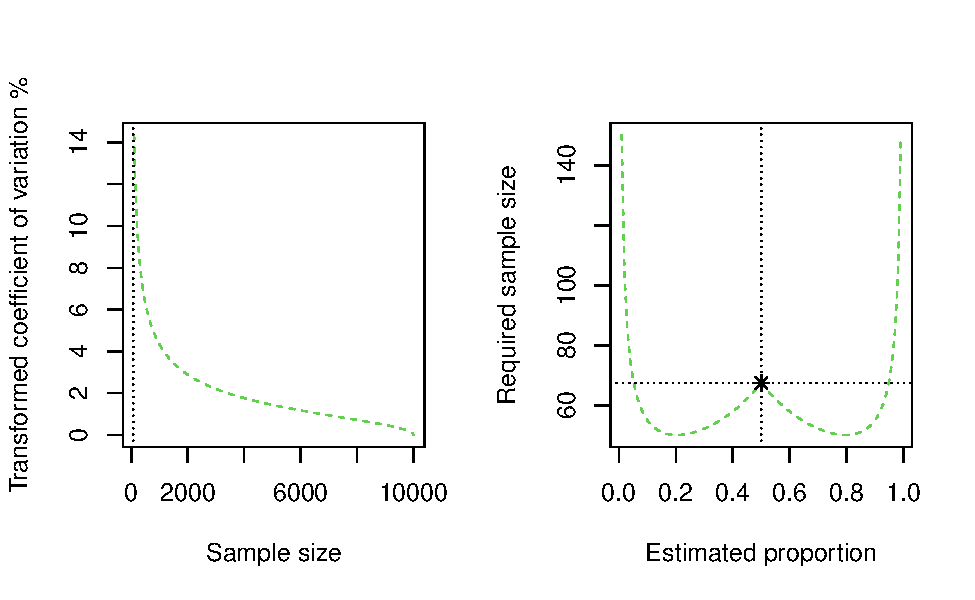
\includegraphics{19Calidad_files/figure-latex/fig1fig-1.pdf}
\caption{\label{fig:fig1fig}Relación entre el tamaño de muestra y la precisión de un indicador utilizando la transformación Logit.}
\end{figure}

La figura \ref{fig:fig1fig} muestra que, al igual que con el coeficiente de variación original, el tamaño de muestra aumentará a medida que se requiera mayor precisión en la estimación; pero a diferencia del coeficiente de variación original, el tamaño de muestra será idéntico para los fenómenos que induzcan proporciones simétricas. Además, el tamaño de muestra necesario para estimar eficientemente una proporción \(P\leq 0.5\) con una precisión mayor a un determinado umbral del coeficiente de variación \(CVE\) es:

\[
n \geq \dfrac{P \ (1-P) \  DEFF}{\frac{P \  (1-P) \ DEFF}{N}+\log^2\ (P) \ P^2 \ CVE^2}
\]

La expresión anterior se obtiene teniendo en cuenta el siguiente desarrollo algebraico. En particular, cuando \(P > 0,5\), se desea que el coeficiente de variación logarítmico sea menor a un umbral \(\delta\) y, por lo tanto, habiendo definido \(S^2 = P\ (1-P) \  DEFF\), se tiene la siguiente implicación.

\[
CV(\hat{L}) \leq \delta 
\Longrightarrow
n \geq \frac{S^2}{\ \delta^2(1-\hat{P})^2\log^2(1-\hat{P}) +\frac{S^2}{N}}
\]

Análogamente, cuando \(P \leq 0.5\), se tiene que

\[
CV(\hat{L}) \leq \delta
\Longrightarrow
n \geq \dfrac{S^2}{\frac{S^2}{N}+\log^2(\hat{P})\hat{P}^2\delta^2}
\]

\hypertarget{el-efecto-de-diseuxf1o-deff}{%
\subsection{El efecto de diseño DEFF}\label{el-efecto-de-diseuxf1o-deff}}

Cuando se selecciona una muestra utilizando un diseño de muestreo complejo es muy improbable que exista independencia entre las observaciones. Además, como el muestreo de las encuestas de hogares es complejo, la distribución de la variable de interés no es la misma para todos los individuos. Por lo anterior, cuando se analizan datos que provienen de encuestas de hogares la inferencia correcta debe tener en cuenta estas grandes desviaciones con respecto al análisis estadístico clásico, que considera muestras aleatorias simples. Por ello, en la mayoría de ocasiones se necesita aumentar el tamaño de muestra para obtener la precisión deseada.

\citet{Lumley_2010} afirma que el efecto del diseño compara la varianza de una media o total con la varianza de un estudio del mismo tamaño utilizando un muestreo aleatorio simple sin reemplazo y que su cálculo será incorrecto si los pesos de muestreo se han re-escalado o no son recíprocos a las probabilidades de inclusión. Además, en \texttt{R} se compara la varianza de la estimación con la varianza de una estimación basada en una muestra aleatoria simple del mismo tamaño que el de la subpoblación. Entonces, por ejemplo, en el muestreo aleatorio estratificado, el efecto de diseño calculado en un estrato será igual a uno.

\hypertarget{tamauxf1o-de-muestra}{%
\subsection{Tamaño de muestra}\label{tamauxf1o-de-muestra}}

El tamaño de muestra afecta de manera indirecta la amplitud del intervalo de confianza, a través del error estándar, que generalmente decrece a medida que el tamaño de muestra se hace más grande. Un adecuado tamaño de muestra garantiza la convergencia en distribución de los estimadores a la distribución teórica de donde se calculan los percentiles en el cálculo del intervalo de confianza. En la fase de diseño, es posible mostrar que el tamaño de muestra requerido para estimar el promedio de una variable de interés en una encuesta de hogares, con un error de muestreo relativo menor a \(\delta \in (0,1)\) y una confianza estadística mayor a \(1-\alpha\), está dado por la siguiente expresión.

\[ 
n \geq \dfrac{S^2_{y}\ DEFF}{\dfrac{\delta^2 \  \bar{y}^2}{z_{1-\alpha/2}^2}+\dfrac{S^2_{y}\ DEFF}{N}}
\]

En donde \(z_{1-\alpha/2}\) es el percentil (\(1- \alpha/2\)) asociado a una distribución normal estándar. Por ejemplo, en un diseño de muestreo en varias etapas, si el valor del coeficiente de correlación intraclase es grande, entonces el valor del efecto de diseño DEFF también lo será y por consiguiente el tamaño de muestra deberá ser más grande. Por ejemplo, al medir ingresos en la región, debido a la realidad económica de los países, es común encontrar que las condiciones de la vivienda está altamente asociado con el ingreso de los individuos. Esto quiere decir que los ingresos no están uniformemente dispersos a través de todos los hogares, y por ende el coeficiente de correlación intraclase será alto. Por otro lado, si lo que se quiere estimar es una proporción \(P\), entonces la expresión apropiada para calcular el tamaño de muestra estará dada por

\[ 
n \geq \dfrac{P\ (1-P)\ DEFF}{\dfrac{\delta^2}{z_{1-\alpha/2}^2 }+\dfrac{P\ (1-P) \ DEFF}{N}}
\]

Como se puede apreciar, el tamaño de muestra es un indicador de la calidad de la encuesta, el cual resulta ser muy importante en la etapa de planeación y diseño. Sin embargo se tiene que considerar que:

\begin{itemize}
\tightlist
\item
  Si el parámetro de interés \textbf{sí} fue tenido en cuenta en la planeación de la encuesta con el propósito de tener representatividad sobre una subpoblación, entonces el tamaño de muestra será apropiado y, por ende, el error de muestreo estará controlado, al igual que el coeficiente de variación, el intervalo de confianza y la precisión de la inferencia será óptima.
\item
  Si el parámetro de interés \textbf{sí} fue tenido en cuenta en la planeación de la encuesta, pero hubo una alta tasa de no respuesta, entonces el tamaño de muestra será mucho menor al planeado inicialmente y, por ende, el error de muestreo será más alto, al igual que el coeficiente de variación, y el intervalo de confianza será muy ancho, haciendo que la precisión de la inferencia no sea apropiada.
\item
  Si el parámetro de interés \textbf{no} fue contemplado en la planeación y diseño de la encuesta de hogares, entonces es posible que el tamaño de muestra sea menor al necesario y, por ende, el error de muestreo será mayor, junto con el coeficiente de variación; por ende, el intervalo de confianza será más amplio y la precisión de la inferencia será deficiente.
\end{itemize}

\hypertarget{tamauxf1o-de-muestra-efectivo}{%
\subsection{Tamaño de muestra efectivo}\label{tamauxf1o-de-muestra-efectivo}}

El principio general detrás de esta medida está supeditado a que en la inferencia propia de las encuestas de hogares con diseños de muestreo complejos no existe una sucesión de variables que sean independientes e idénticamente distribuidas. Por lo tanto, si se piensa en la muestra \((y_1, \ldots, y_n)\) como un vector en el espacio \(n\)-dimensional, el estándar clásico de la teoría estadística asumiría que cada componente del vector puede variar por sí mismo. Sin embargo, debido a la forma jerárquica de la selección de los hogares y a la interrelación de la variable de interés con las UPM, la variabilidad de la inferencia en las encuestas complejas tiene un fuerte componente asociados al mismo conglomerado, por lo que la dimensión final del vector \((y_1, \ldots, y_n)\) es mucho menor que \(n\). De esta forma, se ha definido el tamaño de muestra efectivo \citep[capítulo 6]{United_Nations_2005} como sigue
\[
n_{eff} = \frac{n}{DEFF}
\]

En resumen, el diseño clásico de las encuestas de hogares consiste en seleccionar un conjunto de hogares dentro de una misma UPM y repetir esta estrategia de selección sistemáticamente en todo el país. Por lo tanto, se puede pensar en que, si la variable de interés tiene una alta correlación intraclase, entonces la realidad de las personas y de los hogares dentro de una misma UPM será muy homogénea, tanto que se podría interpretar como que la información estuviese repetida, y que los individuos u hogares de una misma UPM no estuvieran aportando de manera diferenciada. Por lo tanto, debido a los efectos del diseño de muestreo complejo, la cantidad de individuos que están aportando a la inferencia del indicador no es el número de personas, ni el número de hogares en la muestra, sino el tamaño de muestra efectivo \(n_{eff}\), que deflacta los efectos de aglomeración.

\hypertarget{grados-de-libertad}{%
\subsection{Grados de libertad}\label{grados-de-libertad}}

La amplitud del intervalo de confianza de un indicador no sólo está supeditada al error estándar, sino también al percentil de la distribución \(t-student\) con sus correspondientes grados de libertad. De esta manera, entre más grados de libertad se consideren, menor será la amplitud del intervalo y mayor será la precisión de la inferencia. En el caso más general en donde la subpoblación sea toda la población objetivo, los grados de libertad se reducen a la siguiente expresión:

\[
gl = \# UPM - \# Estratos
\]

Los grados de libertad constituyen una medida de cuántas unidades independientes de información se tienen en la inferencia. Nótese que, en el caso extremo de realizar un censo en cada UPM, sin importar el número de individuos que componen el conglomerado, el número de unidades independientes será únicamente el número de UPM seleccionadas en la primera etapa de muestreo puesto que la UPM es la unidad de muestreo que contribuye en mayor medida a la variabilidad de las estimaciones. En las aplicaciones reales de encuestas de hogares, en donde se realiza un submuestreo dentro de la UPM, la variabilidad de la estimación puede verse como la contribución del conglomerado a la gran media, más una contribución (considerada insignificante) de la segunda etapa de muestreo. Nótese la importancia de utilizar la distribución \(t-student\) como base inferencial para la construcción de los intervalos de confianza. Recuérdese además que el percentil 0.975 para la distribución \(t-student\) varía con respecto a sus grados de libertad.

A nivel desagregado, los grados de libertad son determinantes a la hora de hacer inferencias dentro de subpoblaciones de interés. En este caso los grados de libertad no se consideran fijos sino variables. \citet[p.~209]{Korn_Graubard_1999} proponen el siguiente método de cálculo sobre los grados de libertad en una subpoblación \(U_g\):

\[
gl_{g} = \sum_{h=1}^H v_h*(n_{Ih}^g - 1)
\]

En donde \(v_h\) es una variable indicadora que toma el valor uno si el estrato \(h\) contiene uno o mas casos de la subpoblación de interés y toma el valor cero en otro caso, \(n_{Ih}^g\) es el número de unidades primarias de muestreo en el estrato \(h\) \((h=1, \ldots, H)\) con uno o más casos de la subpoblación.

\hypertarget{conteo-de-casos-no-ponderado}{%
\subsection{Conteo de casos no ponderado}\label{conteo-de-casos-no-ponderado}}

El número de casos no ponderados en una muestra es simplemente el conteo de los individuos dentro de la muestra que son afectados por un fenómeno de interés en estudio. Esta cifra está supeditada únicamente a razones y proporciones y tiene un efecto indirecto en la determinación de la precisión del estimador de interés y está determinada por la siguiente expresión.

\[
n_y = \sum_{s}\delta_{k}^y
\]

En donde \(\delta_{k}^y\) es una variable indicadora sobre cada individuo \(k\) de la muestra \(s\) que toma el valor de uno si el individuo está afectado por el fenómeno inducido por la variable de interés \(y\). Nótese que esta es una cantidad aleatoria por definición, y también puede ser calculada en la muestra de un subgrupo poblacional específico \(U_g\), de la siguiente manera:

\[
n_y^g = \sum_{s}z_{g_k}\delta_{k}^y = \sum_{s_g}\delta_{k}^y
\]

Si la incidencia del fenómeno es muy baja (cuando la proporción \(P\) es cercana a cero), tanto el coeficiente de variación original y su transformación logarítmica tendrán magnitudes altas, puesto que:

\[
\lim_{n_y \rightarrow 0} CV(\hat \theta) = 
\lim_{n_y \rightarrow 0} CV(\hat L) = \infty
\]

En muchos países las encuestas de hogares son usadas por las autoridades gubernamentales para asignar recursos a una población potencial. En estos casos, es de particular interés conocer el número de personas que serán susceptible de participar en la repartición de recursos. Por ende, si la estimación de la incidencia total del fenómeno en la población no es precisa, difícilmente se podrá establecer un rubro presupuestal para atender a esta población. Por ejemplo, si la estimación del total de personas afectadas por el fenómeno es del orden de 5\% y su margen de error es 5\%, entonces el coeficiente de variación será de 100\% y el intervalo de confianza de la proporción será \((0 \%, 10 \%)\), demasiado amplio para tomar algún tipo de decisión sobre los recursos públicos de un país. Nótese que esta amplitud se magnifica cuando el número de casos no ponderado no es suficiente.

\hypertarget{criterios-de-calidad-en-subpoblaciones}{%
\section{Criterios de calidad en subpoblaciones}\label{criterios-de-calidad-en-subpoblaciones}}

En esta sección se abordan temáticas referentes al procesamiento apropiado de los indicadores de interés en las subpoblaciones y, habiendo realizado las estimaciones y calculado sus respectivos criterios de calidad, se plantea la utilización de umbrales apropiados para la supresión, revisión o publicación de cifras.

El análisis apropiado de las estadísticas generadas a partir de las encuestas de hogares debe pasar por una definición clara tanto de las subpoblaciones sobre las cuales se quiere realizar la inferencia, como de las variables que generan el indicador de interés. De hecho, como se mostrará más adelante, algunas variables pueden definir una subpoblación y, por ende, es posible que se dé lugar a confusiones. Para aclarar esto, se proponen a continuación algunos ejemplos que permiten dilucidar el cálculo de las medidas de calidad sobre un conjunto no exhaustivo de indicadores de interés.

\textbf{Promedio del ingreso per cápita en el país}

En este caso la variable de interés es una característica continua \(y_k \geq 0 \ \ \ (\forall k \in U)\) definida sobre toda la población del país, mientras que el indicador se escribe como una razón.

\[
\hat {\bar y}_{nacional} = \frac{\hat t_y}{\hat N} =\frac{\sum_h\sum_i\sum_k w_ky_{k}}{\sum_h\sum_i\sum_k w_k}
\]

En donde los subíndices \(h\), \(i\) y \(k\), se refieren a los estratos, las UPM y los individuos, respectivamente. Nótese que la variable que define la población es siempre determinista puesto que \(z_{g_k} = 1\) para todos los individuos que residen en el país, es decir para todos lo individuos de la muestra. En este caso se tiene que los grados de libertad corresponden a todas las UPM menos todos los estratos de la encuesta en el país.

\textbf{Promedio del ingreso per cápita en una ciudad}

En este caso la variable de interés está definida sobre un subgrupo poblacional \(U_g\), correspondiente a la ciudad de interés. El estimador del indicador se escribe como una razón.

\[
\hat {\bar y}_{ciudad}= \frac{\hat t_{y_g}}{\hat N_g} =\frac{\sum_h\sum_i\sum_k w_kz_{g_k}y_{k}}{\sum_h\sum_i\sum_k w_kz_{g_k}}
\]

Nótese que la variable que define la subpoblación es dicotómica dada por

\[ 
z_{g_k}=
\begin{cases}
1, \ \text{Si $k$ reside en la ciudad $U_g$} \\
0, \ \text{en otro caso}
\end{cases}
\]

En este caso el tamaño de muestra es \(n_g = \sum_s z_{g_k}\), es decir el tamaño de muestra de la ciudad; los grados de libertad corresponden a todas las UPM en la ciudad menos todos los estratos en la ciudad.

\textbf{Proporción de personas pobres en el área urbana}

En este ejemplo, el estimador del indicador se escribe como una razón sobre el área urbana \(U_g\).

\[
\hat{P}_{urbano} = \frac{\hat t_{y_g}}{\hat N_g} =\frac{\sum_h\sum_i\sum_k w_kz_{g_k}y_{k}}{\sum_h\sum_i\sum_k w_kz_{g_k}}
\]

En donde \(y_{k}\) es la variable de interés que define una característica dicotómica de la siguiente manera
\[
y_k=
\begin{cases}
1, &\text{si el ingreso per cápita de la persona está por debajo de la línea de pobreza}\\
0, &\text{en otro caso.}
\end{cases}
\]

Las mediciones se realizan sobre la subpoblación definida por la siguiente variable

\[
z_{g_k}=
\begin{cases}
1, &\text{si la persona reside en el área urbana $U_g$}\\
0, &\text{en otro caso.}
\end{cases}
\]

En este caso el tamaño de muestra es \(n_g = \sum_s z_{g_k}\), es decir el tamaño de muestra del área urbana; los grados de libertad corresponden a todas las UPM del área urbana menos todos los estratos del área urbana.

\textbf{Tasa de desocupación nacional}

Este indicador está definido como la división entre el total de personas desocupadas sobre el total de personas activas en la fuerza de trabajo. El estimador del indicador está definido como una razón de dos estimadores de totales poblacionales:

\[
\widehat{TD}_{nacional} =  \frac{\hat t_y}{\hat t_z} =\frac{\sum_h\sum_i\sum_k w_kz_{k}y_{k}}{\sum_h\sum_i\sum_k w_kz_{k}}
\]

En donde la variables de interés toman la siguiente forma
\[
y_{k}=
\begin{cases}
1, &\text{si el individuo es desocupado,}\\
0, &\text{si el individuo no es desocupado,}\\
NA, &\text{si no está en edad de trabajar.}
\end{cases}
\]

Y la variable que define la subpoblación es
\[
z_{k}=
\begin{cases}
1, &\text{si el individuo es activo,}\\
0, &\text{si el individuo es inactivo,}\\
NA, &\text{si el individuo no está en edad de trabajar.}
\end{cases}
\]

En este caso el tamaño de muestra es \(n = \sum_s z_{k}\), es decir el número de personas en la muestra que están en edad de trabajar y son activas. Los grados de libertad corresponden a todas las UPM menos todos los estratos de la encuesta en el país en los que se encontraron hogares con individuos en edad de trabajar y activas. Nótese que estos son los mismos grados de libertad inducidos por la tasa de ocupación. Además, el conteo de casos no ponderado corresponde al número de individuos desocupados en la muestra.

\textbf{Tasa de desocupación masculina en migrantes}

Este indicador está definido como la división entre el total de hombres migrantes desocupados sobre el total de hombres migrantes activos. El estimador del indicador está definido como una razón de dos estimadores de totales poblacionales:

\[
\widehat{TD}_{hombre-migrante} =  \frac{\hat t_{y_g}}{\hat t_{z_g}} =\frac{\sum_h\sum_i\sum_k w_kz_{g_k}y_{k}}{\sum_h\sum_i\sum_k w_kz_{g_k}}
\]

En donde la variables de interés toman la siguiente forma
\[
y_{k}=
\begin{cases}
1, &\text{si el individuo es desocupado,}\\
0, &\text{si el individuo no es desocupado,}\\
NA, &\text{si no está en edad de trabajar.}
\end{cases}
\]

Y la variable que define la subpoblación es
\[
z_{g_k}=
\begin{cases}
1, &\text{si el individuo es activo, hombre y migrante,}\\
0, &\text{si el individuo es inactivo, hombre y migrante}\\
NA, &\text{si el individuo no está en edad de trabajar, o es mujer o es no migrante.}
\end{cases}
\]

En este caso el tamaño de muestra es \(n = \sum_s z_{g_k}\), es decir el número de personas en la muestra que están en edad de trabajar, son hombres migrantes y están activos. El conteo no ponderado de casos corresponde al número de individuos en la muestra que son hombres migrantes y están desocupados. Además, los grados de libertad corresponden a todas las UPM menos todos los estratos de la encuesta en el país en los que se encontraron hogares con hombres migrantes y activos en la fuerza de trabajo.

\hypertarget{secuencia-luxf3gica-para-crear-reglas-de-supresiuxf3n}{%
\section{Secuencia lógica para crear reglas de supresión}\label{secuencia-luxf3gica-para-crear-reglas-de-supresiuxf3n}}

En esta sección se ha querido enfatizar el hecho de que la precisión de una estimación recae directamente en los intervalos de confianza, los cuales pueden ser descompuestos en elementos fundamentales que permiten crear una secuencia lógica de revisión, publicación o supresión de cifras. Nótese que lo anterior se basa en que la longitud de los intervalos de confianza induce la seguridad de que un estimador es o no es preciso. Considere los siguientes ejemplos prácticos:

\begin{itemize}
\tightlist
\item
  La incidencia de la pobreza en un departamento de un país se estimó en \(5,2\)\%, con un intervalo de confianza de (\(5,15\)\%, \(5,25\)\%).
\item
  La tasa de desocupación en el país para los hombres se ubicó en \(7,5\)\%, con un intervalo de confianza de (\(7,1\)\%, \(7,9\)\%); mientras que para las mujeres se ubicó en \(9,2\)\%, con intervalo de confianza de (\(8,8\)\%, \(9,6\)\%).
\item
  La tasa de asistencia neta estudiantil en primaria para el último quintil de ingreso se estimó en \(85\)\%, con un intervalo de confianza de (\(48,2\)\%, \(100,0\)\%).
\end{itemize}

Claramente, en la última situación ejemplificada, el intervalo de confianza no brinda la precisión adecuada para que una Oficina Nacional de Estadística publique esta cifra confiadamente, o para que un gobierno pueda realizar algún tipo de política pública educativa, y mucho menos para estimar los recursos que una de intervención estatal sobre la población de interés. Como se ha descrito a lo largo de este documento, utilizar únicamente el coeficiente de variación como estándar para la supresión de cifras es un criterio que no tiene en cuenta toda las variantes asociadas a la inferencia en un muestreo complejo. A continuación se incorporan algunas recomendaciones internacionales que incorporan otros criterios adicionales a este.

\begin{itemize}
\tightlist
\item
  \textbf{Coeficiente de variación}: \citet{CepalSAe2018} realizó una revisión de las experiencias internacionales, con base en la información publicada en las páginas web de los INE, para determinar cómo son usados los criterios de supresión de información y los umbrales que las oficinas nacionales de estadística definen para la validación de las cifras. Para encuestas de hogares, se encontró que Estados Unidos y los países del Mercosur utilizan un umbral de \(CV > 30\%\), Canadá y México usan como referencia un umbral del \(CV > 25\%\), Chile y Costa Rica utilizan un umbral del \(CV > 20\%\), Ecuador y Perú utilizan un umbral del \(CV > 15\%\), mientras que Colombia usa un umbral del \(CV > 10\%\). De esta forma, cualquier cifra estimada cuyo coeficiente de variación sea mayor al umbral predefinido es suprimida o marcada como una cifra poco confiable.
\item
  \textbf{Tamaño de muestra}: este criterio debe ser considerado como uno de los más importantes a la hora de decidir la ruta de publicación de una cifra, puesto que los desarrollos teóricos en términos de inferencia estadística para encuestas dependen de este término. La cobertura de los intervalos de confianza y la distribución de los estimadores dependen de qué tanto el tamaño de la subpoblación como su tamaño de muestra asociado no sean pequeños. En este espíritu, \citet{Barnett_Walker_Chromy_Davis_Emrich_Odom_Packer_2003} proponen que todas las estimaciones basadas en un tamaño de muestra menor a 100 unidades deberían ser suprimidas o marcadas como no confiables.
\item
  \textbf{Tamaño de muestra efectivo}: al igual que con el anterior criterio, el tamaño de muestra efectivo induce que las aproximaciones teóricas, en términos de convergencia de las distribuciones de los estimadores y la cobertura de los intervalos de confianza, se cumplan. \citet{Hornik_Maklan_Cadell_Prado_Barmada_Jacobsohn_Orwin_Sridharan_Zador_Southwell_etal} consideran que si el tamaño de muestra efectivo no es mayor a 140, entonces la cifra no debería ser considerada para publicación. Por otro lado, teniendo en cuenta el tamaño de muestra inducido por la transformación logarítmica, \citet{Barnett_Walker_Chromy_Davis_Emrich_Odom_Packer_2003} afirman que cuando la proporción se encuentra entre \(0.05\) y \(0.95\), entonces el tamaño de muestra efectivo es máximo cuando \(P = 0,5\), siendo su valor \(n_{eff} = 68\).
\item
  \textbf{Conteo de casos no ponderado}: cuando la incidencia de un fenómeno es muy baja y el diseño de la encuesta no lo tuvo en cuenta, entonces es posible que las estimaciones asociadas a tamaños, totales y proporciones sobre este fenómeno no sean confiables. En particular, para las proporciones es posible restringir las estimaciones tales que \(\hat P <0,001\), pero es más expedito crear una regla a partir del conteo de casos en la muestra. Por ejemplo, \citet{AmericanCommunitySurvey} plantea que si el número de casos no ponderados es menor a 50 unidades entonces la estimación no es publicada.
\item
  \textbf{Grados de libertad}: este criterio apunta a aislar el efecto inflacionario del tamaño de muestra en una encuesta compleja y plantea una aproximación al número de unidades independientes en la inferencia. Además, a medida que crece, la amplitud del intervalo de confianza se estabiliza. \citet{Parker_Talih_Malec_2017} consideran que si los grados de libertad inducidos por la subpoblación son menos de ocho, la cifra debería ser suprimida.
\item
  \textbf{Coeficiente de variación logarítmico}: Esta medida de suavizamiento toma valores altos cuando las proporciones estimadas están demasiado cercanas a cero o a uno. \citet{Barnett_Walker_Chromy_Davis_Emrich_Odom_Packer_2003} proponen que la cifra debe ser suprimida si el coeficiente de variación logarítmico es mayor que 17.5\%.
\end{itemize}

Nótese que los criterios mencionados en este documento no deberían ser aplicados de manera independiente, sino que tendrían que seguir cierta lógica, puesto que es posible, por ejemplo para una variable con poca homogeneidad en las UPM, que con un tamaño de muestra de \(n=90\), se haya estimado un efecto de diseño de \(DEFF=0,5\), lo cual implicaría un tamaño de muestra efectivo de \(n_{eff}=180\). En este caso, si los criterios de supresión se aplicaran de manera independiente, se concluiría que la cifra debería ser suprimida por tener un tamaño de muestra insuficiente, pero a la vez, que la cifra debería ser publicada, por tener un tamaño de muestra efectivo suficiente. Lo anterior, podría llevar a contradicciones por parte de los INE y malas interpretaciones por parte los usuarios finales de los datos.

De manera general, se recomienda que los INE estudien a profundidad sus políticas de supresión, revisión y publicación de cifras en cada una de las encuestas que realiza y, de manera independiente, defina las reglas apropiadas para cada caso y que los criterios de supresión sean plasmados en forma de diagrama de flujo en la documentación de las encuestas. Además, cada encuesta debería considerar un algoritmo de forma particular; es decir, los criterios de supresión no necesariamente deben coincidir para cada operación estadística, aunque sí debiesen acogerse unos mínimos en cada ONE para garantizar la calidad de la estimaciones publicadas provenientes de las encuestas de hogares.

Teniendo en cuenta las particularidades de la región, en este documento se recomienda mantener un umbral del coeficiente de variación \(CV > 20\%\) y del coeficiente de variación logarítmico \(CV(\hat{L}) > 17.5%
\) como generadores de alertas sobre la calidad de la estimación; además se recomienda tener mínimo 14 grados de libertad, los cuales implican al menos 15 UPM que inducirían una convergencia en la distribución del estimador \citep[figura 8.1]{Gutierrez_2016}. A partir de esta cifra es posible continuar el análisis de las recomendaciones con las particularidades de cada encuesta en cada país. Por ejemplo, \# si se espera un mínimo de 15 UPM, y en cada una se seleccionan 12 hogares, entonces la muestra esperada es de 180 hogares, y tomando una tasa de efectividad del 85\%, esta se reduce a \(n < 153\) como generados de alertas. Asimismo, tomando en cuenta un efecto de diseño promedio de 2.5 (calculado según el indicador de interés), se obtendría un tamaño de muestra efectivo de \(n_{eff} = 61\) como generador de alertas. Asimismo, se recomienda mantener el conteo de casos no ponderado en \(n_y < 40\) e inmediatamente generar una alerta sobre todas las cifras que reporten un efecto de diseño \(DEFF < 1\).

Por ejemplo, la figura \ref{fig:figCSj1} muestra una propuesta preliminar, para la estimación de proporciones o razones, en cuanto a los criterios de supresión de cifras. En una primera instancia se realiza la estimación clásica de los parámetros de interés y se genera una tabla que adjunte el cálculo de todos los criterios descritos anteriormente. Luego, dependiendo de la naturaleza del fenómeno investigado, se deben establecer los criterios que se van a tener en cuenta y los umbrales en cada caso. El próximo paso es decidir, para cada cifra de la tabla generada, si se va a publicar o suprimir, y en algunos casos si se revisará la cifra con mayor detenimiento. Por ejemplo, en el diagrama propuesto se definen seis criterios como condiciones necesarias para la publicación inmediata de una cifra; los primeros cuatro, son condiciones necesarias para la revisión temática. Si alguno de los primeros cuatro criterios no se satisface, entonces la cifra es suprimida.

\begin{figure}
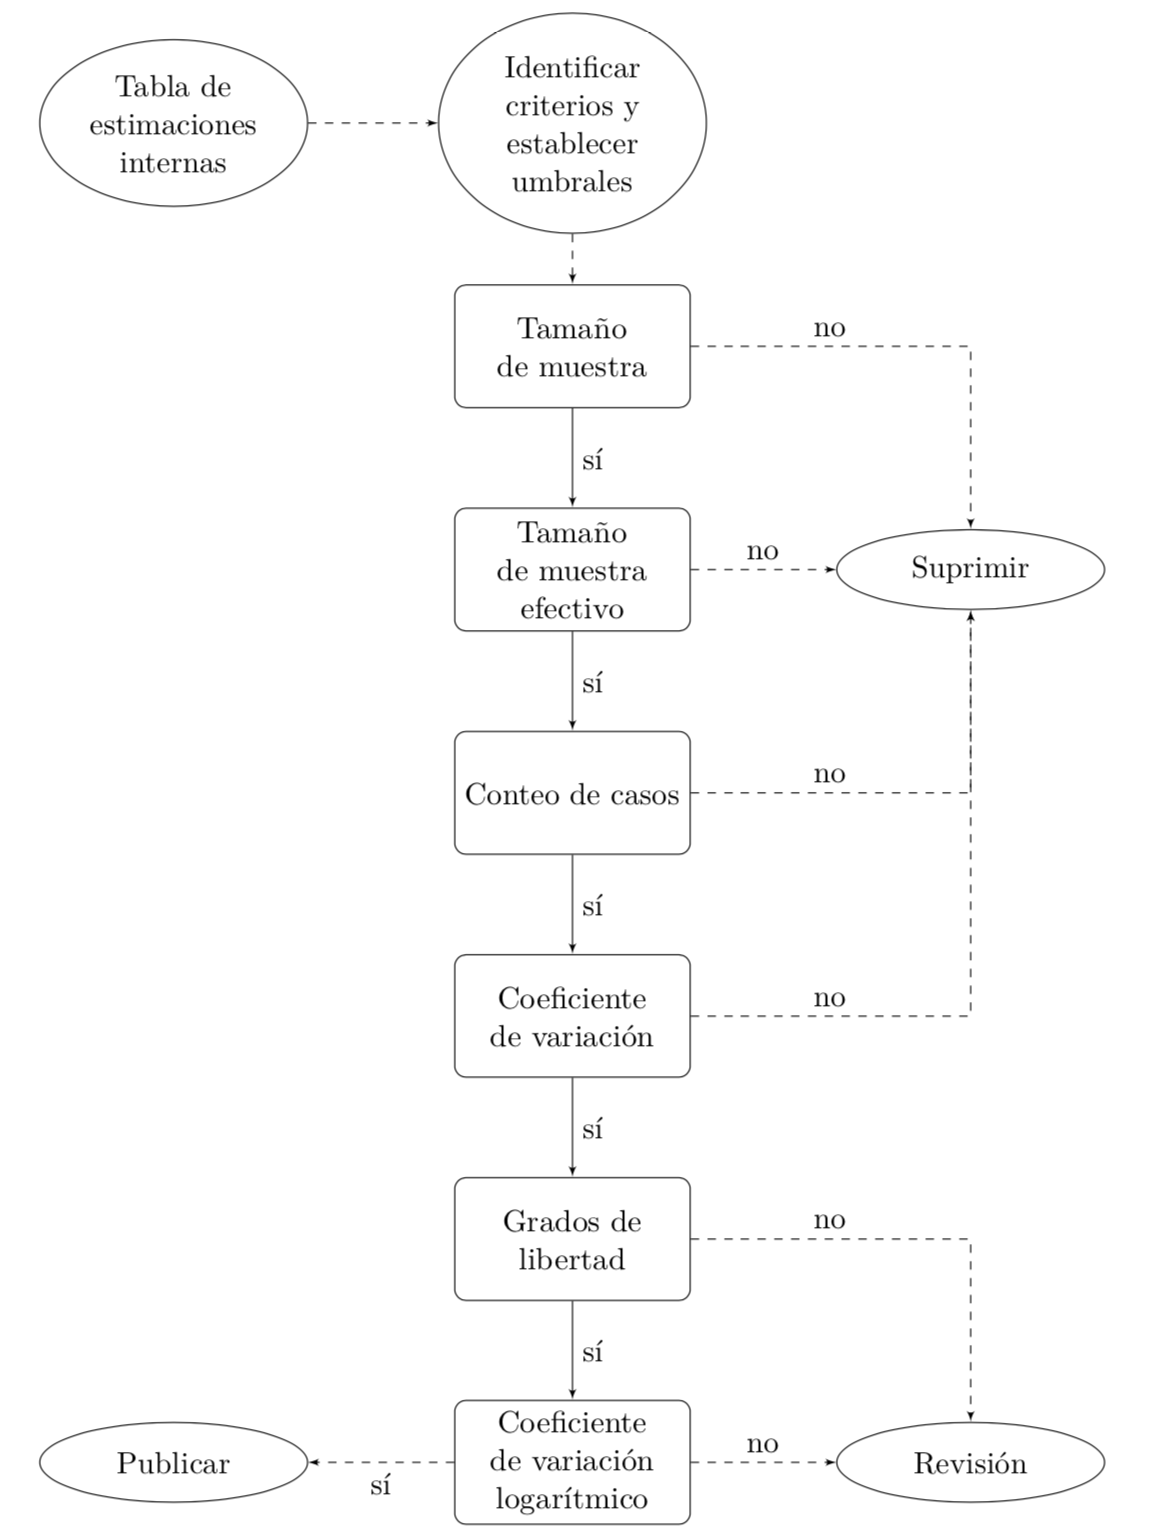
\includegraphics[width=0.5\linewidth]{Pics/CSj1} \caption{Ejemplo de un diagrama de flujo para la publicación, supresión y revisión de estimaciones de proporciones o razones en encuestas de hogares.}\label{fig:figCSj1}
\end{figure}

\hypertarget{comparabilidad-rediseuxf1o-impacto-y-empalme}{%
\chapter{Comparabilidad: rediseño, impacto y empalme}\label{comparabilidad-rediseuxf1o-impacto-y-empalme}}

Entre los objetivos más importantes de las Oficinas Nacionales de Estadística se encuentra el ser garantes de la comparabilidad de las estadísticas oficiales publicadas regularmente. Como se ha visto a los largo de todo este libro, entendemos una estrategia de muestreo como una dupla compuesta por un diseño de muestreo y un estimador. Desde un punto de vista estadístico esta dupla crea una medida de probabilidad discreta que induce las estimaciones de las estadísticas oficiales que serán publicadas y diseminadas por las ONE mediante la realización de las encuestas de hogares. Esta medida de probabilidad no solo induce la estimación puntual del parámetro de interés, sino que a su vez induce una estimación de su varianza y error de muestreo, que a su vez redunda en una inferencia completa y correcta.

La estabilidad en el tiempo de la medida de probabilidad de las encuestas de hogares trae grandes ventajas, pues además de poder realizar comparaciones transversales entre subgrupos poblacionales de interés (región, zona, sexo, edad, escolaridad, discapacidad, etnia, entre muchos otros), será también posible realizar comparaciones temporales de dichos subgrupos. Uno de los ejemplos más ampliamente difundidos son los parámetros del mercado de trabajo (tasa de desocupación, tasa de participación, tasa de informalidad, entre otros), cuya importancia es tal que las ONE disponen de levantamientos continuos para poder estimarlos y diseminar su publicación regularmente (de forma trimestral, o incluso mensual). La comparación temporal de estas cifras permite el planteamiento de políticas públicas oportunas.

Por ende, el cambio de alguno de los componentes de la estrategia de muestreo afectará de alguna manera la comparabilidad de las estadísticas oficiales en algunos puntos del tiempo y, si el efecto es significativo, incluso podrá poner en tela de juicio la idoneidad de la inferencia para la estimación de los parámetros de interés. Por ejemplo, considere que, debido a la coyuntura socioeconómica de un país, efectivamente hay un cambio negativo en el mercado de trabajo en un periodo de interés; pero este cambio no podrá ser debidamente captado si existe algún cambio simultaneo en el diseño de muestreo (que a su vez viene inducido por la forma en que se recolecta la información) o en el estimador de muestreo (debido cualquier cambio en el ajuste a los factores de expansión incluyendo los modelos de ausencia de respuesta y calibraciones).

Por la evolución natural de las encuestas, la adopción de nuevas metodologías de medición, el cambio en la forma de recolección de la información o incluso la adopción de nuevas proyecciones censales por la realización decenal de los censos de población y vivienda, es casi una tarea imposible no realizar ningún cambio en la vida de las encuestas de hogares. En este capítulo describiremos cuál es la mejor manera de realizar estos cambios para minimizar su impacto, cómo medir este efecto en el tiempo y, llegado el caso, cómo hacer comparables las series de tiempo que han sufrido una discontinuidad en un punto del tiempo debido a un cambio en la medida de probabilidad.

\hypertarget{rediseuxf1o-de-las-encuestas}{%
\section{Rediseño de las encuestas}\label{rediseuxf1o-de-las-encuestas}}

Aunque la comparabilidad de las estimaciones es un baluarte fundamental en la diseminación y publicación de las estadísticas oficiales provenientes de las encuestas de hogares, es casi imposible mantener intacta la medida de probabilidad de la inferencia a lo largo del tiempo. Las encuestas de hogares son frecuentemente rediseñadas para reflejar los cambios relacionados con la población de interés. Estos rediseños son necesarios para mantener la eficiencia de la estrategia de muestreo e incorporar mejoras metodológicas optimas. A continuación, se enumeran algunos casos en los que puede existir un cambio que afecte la comparabilidad:

\begin{enumerate}
\def\labelenumi{\arabic{enumi}.}
\tightlist
\item
  \emph{Cambios en la forma de medición de los constructos}; es posible encontrar que la forma en que se miden los constructos cambien a través del tiempo. Por ejemplo, la concepción y definición de las fuentes del ingreso \citep{CEPAL_2018} para mediciones de pobreza monetaria o la actualización de los estándares de la Organización Internacional del Trabajo \citep{ILO_2013} en cuanto a la definición de los indicadores del mercado laboral, son algunos casos en los que los cuestionarios deben sufrir modificaciones para poder tener una inferencia oportuna.
\item
  \emph{Cambios en la definición de las subpoblaciones}; la generación de nuevos estándares sobre la clasificación de las subpoblaciones puede repercutir significativamente en la comparabilidad de las series. Por ejemplo, la adopción de estándares sobre la identificación de razas, etnias o pueblos originarios, además de cambios en la identifiación de migrantes y extranjeros; nuevos estándares sobre identificación de poblaciones con preferencias sexuales y de género diversas; nuevos estándares en la clasificación de las ocupaciones, entre otras.
\item
  \emph{Cambio en la forma de recolección de la información primaria}; con el pasar de los años y la adopción de nuevos procesos tecnológicos en las ONE de la región, es muy probable encontrar que las entrevistas que habitualmente se recolecataban de manera presencial con cuestionarios en papel, poco a poco van migrando a una forma de recolección presencial con dispositivos de captura digitales, e inclusive es posible encontrar cambios más drásticos en los que la recolección puede cambiarse a operativos telefónicos o mixtos. Esta nueva forma de recolección de la información puede traer cambios en la comparabilidad de las series.
\item
  \emph{Cambios en la división territorial del país}; aunque este tipo de cambios no son tan frecuentes, es posible encontrar nuevas definiciones territoriales dentro de los países; por ejemplo, la creación de nuevas divisiones administrativas mayores (regiones, estados o departamentos) y/o menores (municipios, distritos, cantones o provincias). Estos cambios en la división administrativa y territorial de los países pueden redundar en discontinuidades, sobretodo en las estadísticas generadas a nivel subnacional.
\item
  \emph{Cambios debido a la realización de nuevos censos en el país}; la mera realización de los censos puede traer consigo consecuencias inesperadas en la comparabilidad de las series. Por ejemplo:

  \begin{itemize}
  \tightlist
  \item
    La forma en la que se desarrollan los censos tiene una repercusión directa sobre la construcción de los marcos de muestreo, que inducen el diseño de muestreo de la encuesta. Si el censo anterior fue un censo de hecho y el actual es un censo de derecho (o viceversa) la definición y construcción cartográfica de las áreas de enumeración o empadronamiento serán diferentes en su tamaño y composición. Dado que estas áreas son el principal insumo de la creación de las Unidades Primarias de Muestreo, los cambios en la cartografía de los marcos de muestreo serán significativas y acabaran redundando en el quiebre de las series temporales.
  \item
    La actualización de las proyecciones demográficas trae consigo un cambio en los totales de control usados en los estimadores de calibración. Ante un cambio significativo en la población proyectada y la observada en el censo, es muy probable que las estadísticas oficiales de nivel (totales y tamaños, en particular) se vean afectadas por estos cambios y las estadísticas ya no sean comparables, pues se observará un incremento (o decremento) de las proyecciones de la población civil no instucionalizada \citep{BLS_2014}.
  \end{itemize}
\item
  \emph{Mejoras deliberadas}; cualquier otro cambio en la estrategia de muestreo puede traer discrepancias en las series de tiempo. Por ejemplo, una nueva forma de administración del marco de muestreo con nuevos tamaños en las UPM, o la adopción de una nueva estrategia de estratificación socioeconómica de las UPM del marco tendrán un efecto en las cifras. Asimismo, el cambio y mejora en el diseño de muestreo, la adopción de un nuevo estimadores o los cambios realizado en los ajustes de los pesos de muestreo y factores de expansión pueden tener connotaciones inesperadas en la comparabilidad de las cifras.
\end{enumerate}

\hypertarget{el-impacto-de-los-rediseuxf1os}{%
\section{El impacto de los rediseños}\label{el-impacto-de-los-rediseuxf1os}}

Como los rediseños de las encuestas son inevitables, es muy recomendable definir de antemano los cambios que se surtirán y planear un experimento controlado a lo largo de un periodo suficiente de tiempo (por ejemplo, un año para eventos con estacionalidad como las estadísticas del trabajo) en donde la operación estadística transcurra en paralelo con dos acercamientos: el regular (sin cambios) y el nuevo (con los cambios del rediseño). Esta opción implica que la ONE debe tener a su disponibilidad la suficiente cantidad de recursos presupuestales, logísticos y humanos durante el tiempo en el cual transcurran ambos procesos. Por lo anterior, no todas las ONE de la región podrán asumir esta carga y se vuelve una opción inviable. Sin embargo, las autoridades de las ONE deberían realizar todos los esfuerzos posibles para conseguir los recursos suficientes y garantizar que se pueda medir el impacto de los cambios propuestos.

Con base en lo anteriomente mencionado, es necesario tener en cuenta que sin este tipo de experimentos paralelos, será muy difícil medir el verdadero cambio, identificar la fuente de la discontinuidad en la serie y corregir el sesgo generado. Tal como lo afirma \citet{Imbens_Rubin_2015}, la aleatorización es la única forma de conseguir que no existan sesgos de selección en los experimentos controlados y es el único supuesto científicamente aceptado para medir este tipo de efectos. Con esta perspectiva en mente, los experimentos controlados deberán seleccionar aleatoriamente las UPM que participarían en ambas recolecciones. Esto no supone una carga adicional para las ONE, garantes de la aleatorización en las encuestas de hogares.

\citet{Brakel2008} menciona que hay varias posibilidades para llevar a cabo este tipo de experimentos paralelos; por una parte es posible tener dos operaciones estadísticas en campo con el mismo tamaño de muestra, o que la nueva operación tenga un tamaño de muestra menor e inclusive esté restringida a alguna subpoblación de interés. En cualquier caso, son la forma correcta para evitar efectos de confusión. De lo contrario, incluso ante cambios nulos, no se podrá discernir si esto es el resultado de la coyuntura de interés, o del rediseño de la encuesta. La figura \ref{fig:fig201} muestra un ejemplo simulado del resultado esperado de un experimento paralelo. La línea negra representa la serie regular, la linea azul representa la nueva serie con los cambios del rediseño y la distancia entre ambas, representa el impacto del rediseño en cada punto del tiempo.

\begin{figure}
\centering
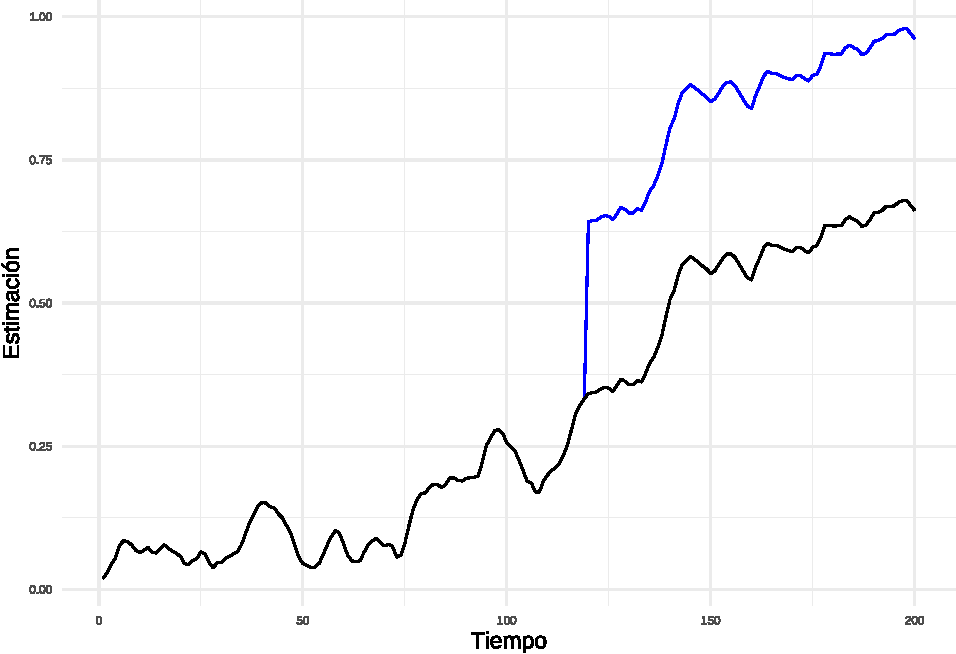
\includegraphics{20Empalme_files/figure-latex/fig201-1.pdf}
\caption{\label{fig:fig201}Series de tiempo para el rediseño de una encuesta. La línea negra representa la serie regular; la línea azul representa la serie nueva. Fuente: elaboración propia.}
\end{figure}

Sin embargo, en algunos casos se hace imposible realizar dos levantamientos paralelos. Un claro ejemplo de este escenario lo tenemos en la pandemia por COVID-19, su efecto en las condiciones socioeconómicas de los hogares y su efecto en el modo de recolección de las encuestas. Como lo afirma \citet{CEPAL_continua}, desde la emergencia sanitaria derivada de la pandemia, las oficinas nacionales de estadística (ONE) tuvieron que interrumpir abruptamente la recopilación de información primaria como parte de muchas de sus operaciones estadísticas, incluidas las encuestas de hogares. A pesar de esto, las ONE pudieron seguir con sus levantamientos migrando de un modo de recolección presencial a telefónico.
Este rediseño repentino (cambio en la metodología de recolección) fue necesario para que se siguieran produciendo cifras de empleo y pobreza, indicadores particularmente importantes en el contexto de la pandemia, dado el profundo impacto que las mismas restricciones de movimiento y cuarentenas tuvieron en la condición de ocupación de las personas de la región y, por ende, en la afectación de sus ingresos. Nótese que en este caso, no fue posible que las ONE pudiesen realizar experimentos paralelos.

\citet{CEPAL_continua} afirma que la pandemia obligó a que los países cambiaran varios aspectos en la metodología del levantamiento y análisis de la información, que pueden ser resumidos a continuación:

\begin{itemize}
\tightlist
\item
  Cambió el modo de levantamiento de presencial a telefónico (o mixto, en algunos casos), así como las definiciones de la estructura de elegibilidad de las viviendas seleccionadas y sus correspondientes códigos de disposición.
\item
  Cambió el esquema de supervisión de los encuestadores y, en algunos casos, se suprimieron las actualizaciones cartográficas del número de hogares particulares en las unidades primarias de muestreo seleccionadas.
\item
  Se introdujo un nuevo esquema de ajuste de factores de expansión, buscando eliminar el sesgo de cobertura (no todos los hogares en los levantamientos anteriores contaron con números telefónicos de contacto) y de ausencia de respuesta (algunos hogares contactados telefónicamente no contestaron el cuestionario).
\item
  Se revisitaron los esquemas de calibración de los factores de expansión y en aras de la flexibilidad de la metodología de estimación se restringió el número de restricciones de calibración.
\end{itemize}

En algunos casos especiales, ante la imposibilidad de ejecutar dos encuestas paralelas, es posible obtener dos series paralelas. Por ejemplo, suponga un cambio en la forma de medición de las estadísticas del mercado de trabajo en un país; en particular, la adopción del estándar CIET 19 \citep{ILO_2013}. En algunos países es posible adoptar este estándar mediante la adición de nuevas preguntas al cuestionario original basado en la CIET 13 \citep{ILO_1982}. Otro caso especial puede deberse a la actualización de las proyecciones de población y los totales de control en los estimadores de calibración. Dado que el cambio solo afecta los procesos computacionales, es posible tener dos series paralelas, sin necesidad de tener dos levantamientos paralelos.

Ya sea que se tenga la posibilidad de contar con dos series en paralelo o no, existirán diferentes métodos que permitirán establecer si existe o no un impacto significativo debido a un cambio en la encuesta. En general, es posible enlistar las siguientes posibilidades:
1. Cuando se tienen las dos series en paralelo es posible cuantificar el impacto a través de estudios de causalidad basado en modelos econométricos.
2. Cuando solo se cuenta con una serie es posible acercarse al efecto del cambio utilizando modelos de series temporales en los que se involucran parámetros que indiquen a partir de qué momento se inició el cambio y su efecto en la serie (análisis de intervenciones).

En ambos casos, es necesario primero realizar este tipo de análisis para cuantificar el efecto del cambio. Luego, si el efecto resulta ser estadísticamente significativo, es necesario realizar el empalme de las series de tiempo que proporcione una serie ajustada comparable con ambas series: la regular y la nueva. Esta se conoce como la serie empalmada.

Por ejemplo, para el caso en el que el indicador de interés sea un total, \citet{Gbur} propone la utilización de un modelo lineal para determinar los efectos del rediseño. Este modelo puede escribirse de la siguiente manera:

\[
\hat \theta_{tdg} = \hat N_{tdg} \ \theta_{td} + \hat N_{tdg} \ \beta_{t} + \varepsilon_{tdg} 
\]

En donde \(\hat \theta_{tdg} = \sum_{k \in s_t} w_{ktg} \ y_{ktg}\) representa la estimación del indicador de interés en el tiempo \(t\) para el dominio \(d\). El subscrito \(g = 1, 2\), solo toma dos valores e indica si la variable de interés fue observada bajo las condiciones del rediseño o no (tratamiento/control). Además, \(\hat N_{tdg} = \sum_{k \in s_t} w_{ktg}\) es la suma de los factores de expansión en el tiempo \(t\), del dominio \(d\) en el tratamiento \(g\). Este modelo relaciona el estimador directo \(\hat \theta_{tdg}\) con el indicador verdadero \(\theta_{tdg}\) y el efecto del rediseño en el tiempo \(y\), denotado por \(\beta_{t}\). Por supuesto, \(\varepsilon_{tdg}\) denota los errores aleatorios con vector de medias nulo y matriz de varianzas \(\boldsymbol V\), cuyas entradas (varianzas y covarianzas) son estimadas a partir de los principios de la estimación directa. Nótese que se supone independencia en la selección de los hogares o personas en cada grupo del tratamiento.

Evidentemente si \(\beta_{t}\) es estadísticamente igual de cero, entonces se afirma que no existe un efecto del rediseño en la serie regular, por ende se garantiza la comparabilidad entre las estimaciones de la serie regular y la serie nueva. Sin emabargo, en caso contrario, es necesario realizar un proceso de empalme de series como los que se especifican en la siguiente sección.

\hypertarget{empalme-de-series-de-tiempo}{%
\section{Empalme de series de tiempo}\label{empalme-de-series-de-tiempo}}

A continuación se realiza un recuento de algunas técnicas que permiten empalmar dos series. Cada uno de los escenarios que se enlistan a continuación deberá ser adoptado a las necesidades de cada ONE y de cada encuesta. En términos de notación, \(\hat \theta^{R}_t\) representa la estimación regular en el tiempo \(t\), \(\hat \theta^{N}_t\) denota la nueva estimación en el tiempo \(t\) y \(\hat \theta^{E}_t\) corresponde a la estimación empalmada en el tiempo \(t\).

\hypertarget{factor-suavizado}{%
\subsection{Factor suavizado}\label{factor-suavizado}}

\citet{DiNatale} presenta el siguiente ajuste que suaviza sistemáticamente el cambio entre la nueva serie en tiempo del rediseño (\(t_b\)) y la serie regular en el punto inmediatamente anterior \(t_b-1\). Es necesario identificar el punto donde ocurrió el cambio \(t_b\), así como el punto que indicará el comienzo del empalme \(t_1\). Luego, se debe calcular el factor de ajuste que representa el cambio (porcentual).
\[
\gamma_t=\left(\frac{\hat \theta^{N}_{t_b}}{\hat \theta^{R}_{t_b-1}} -1\right)  \times \psi_t
\]
Así, suponiendo que \(\psi_t = \frac{t}{t_b-1} \in (0,1)\) es un factor que aumenta a medida que el tiempo se acerca al punto de quiebre \(t_b\), entonces la serie empalmada queda definida como
\[
\hat \theta^{E}_t=\hat \theta^{R}_t* (1+\gamma_t),
\ \ \ \ \ \ \ \ \ \ \ \ \ \ \ \ \ \ \text{con } t=1,2,\cdots,t_b-1.
\]

En la Figura \ref{fig:fig202} es posible observar cómo se empalman las series regular y nueva a partir del ajuste proporcional. Nótese que la estructura de la serie se mantiene integralmente.

\begin{figure}
\centering
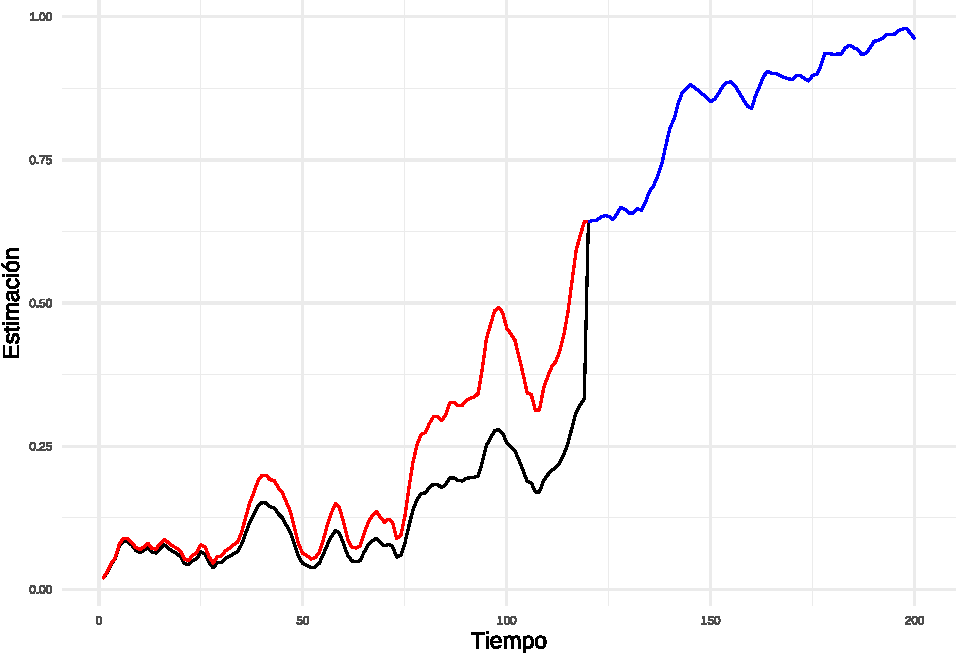
\includegraphics{20Empalme_files/figure-latex/fig202-1.pdf}
\caption{\label{fig:fig202}Empalme de series de tiempo con el método del factor suavizado. La línea negra corresponde a la serie regular; la línea azul representa la serie nueva; la línea roja denota la serie empalmada. Fuente: elaboración propia.}
\end{figure}

\hypertarget{ajuste-sintuxe9tico-aditivo-y-multiplicativo}{%
\subsection{Ajuste sintético aditivo y multiplicativo}\label{ajuste-sintuxe9tico-aditivo-y-multiplicativo}}

En este caso se supone que la serie regular y la serie nueva se observan desde \(t_b\) y que la serie empalmada sigue un ajuste aditivo dado por la siguiente expresión:

\[
\hat \theta^{E}_t=\hat \theta^{R}_t + \left(\hat \theta^{N}_{t_b} - \hat \theta^{R}_{t_b}\right) \times \psi_t
,
\ \ \ \ \ \ \ \ \ \ \ \ \ \ \ \ \ \ \text{con } t=1,2,\cdots,t_b-1.
\]

Este método tiene la desventaja de que la serie empalmada podría producir valores por fuera del rango del indicador de interés; por ejemplo, podria producir valores negativos. Por tanto, para evitar estos inconvenientes, es posible acudir a un empalme sintético multiplicativo, dado a continuación:

\[
\hat \theta^{E}_t=\hat \theta^{R}_t  \left(\dfrac{\hat \theta^{N}_{t_b}}{\hat \theta^{R}_{t_b}}\right)  \times \psi_t 
,
\ \ \ \ \ \ \ \ \ \ \ \ \ \ \ \ \ \ \text{con } t=1,2,\cdots,t_b-1.
\]

\citet{Brakel2008} afirma que con los anteriores métodos la serie empalmada puede ser mayor que uno o menor que cero, lo cual es especialmente contraproducente en el caso de las proporciones y tasas. La Figura \ref{fig:fig203} muestra el empalme de las series usando el ajuste sintético multiplicativo.

\[
\hat \theta^{E}_t=\hat \theta^{R}_t + \left(\hat \theta^{N}_{t_b} - \hat \theta^{R}_{t_b}\right) \times \left( \dfrac{\hat \theta^{R}_t(1-\hat \theta^{R}_t)}{\hat \theta^{R}_{t_b}(1-\hat \theta^{R}_{t_b})}\right) 
,
\ \ \ \ \ \ \ \ \ \ \ \ \ \ \ \ \ \ \text{con } t=1,2,\cdots,t_b-1.
\]

\begin{figure}
\centering
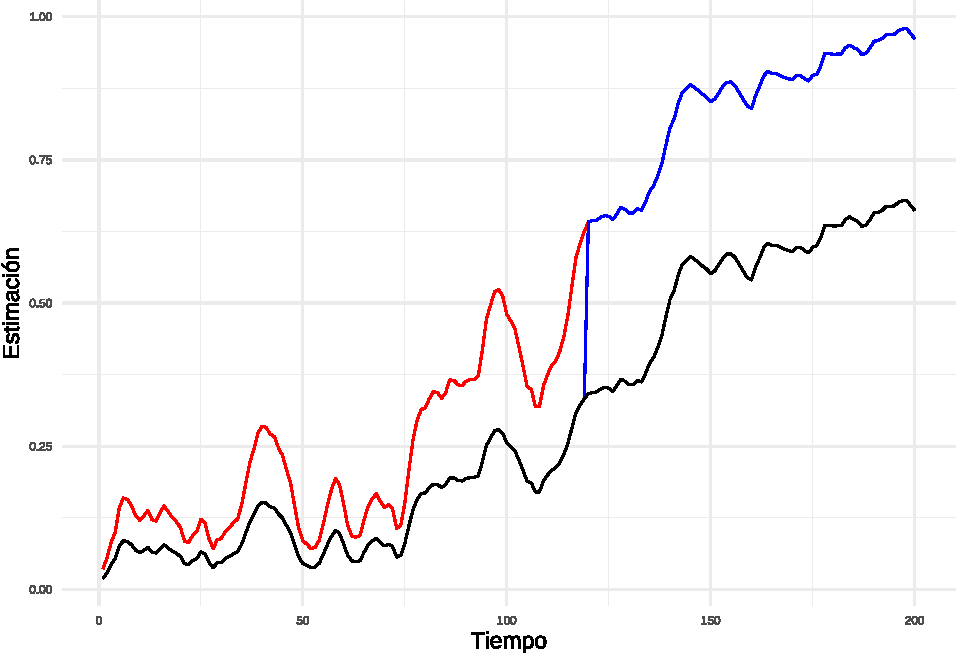
\includegraphics{20Empalme_files/figure-latex/fig203-1.pdf}
\caption{\label{fig:fig203}Empalme de series de tiempo con el ajuste sintético multiplicativo. La línea negra corresponde a la serie regular; la línea azul representa la serie nueva; la línea roja denota la serie empalmada. Fuente: elaboración propia.}
\end{figure}

\hypertarget{modelos-estructurales}{%
\subsection{Modelos estructurales}\label{modelos-estructurales}}

En el caso en el que no se tenga la oportunidad de tener un experimento paralelo y, por lo tanto, se carezca de dos series paralelas, es posible ajustar un modelo estructural de series de tiempo con una intervención justo en el momento del rediseño. Para simplificar la notación, en esta sección se supone que la serie no tiene estacionalidad, ni ciclos; aunque si los tuviera el espíritu del ajuste se mantiene. Por ende, siguiendo a \citet{Brakel2008}, el modelo estructural para la serie está dado por el nivel \(L_t\) más el impacto \(\beta\) en el momento del rediseño \(t_b\) y se escribe de la siguiente manera:

\[
\hat \theta_{t}=L_t+\beta\delta_t+e_t
\]
En donde \(\delta_t\) es una variable indicadora del tiempo en el que se implementó el rediseño en la encuesta

\[
\delta_t =
\begin{cases}
1 & \text{si $t\geq t_b$}\\
0 & \text{si $t< t_b$}
\end{cases}
\]

Además, \(L_t\) es una tendencia estocástica autorregresiva que depende de una pendiente:
\[
\begin{aligned}
L_t & = L_{t-1}+R_{t-1}+w_t \\
R_t & = R_{t-1}+\eta_t
\end{aligned}
\]
Note que \(R_t\) es la pendiente, y \(e_t\), \(w_t\) y \(\eta_t\) son ruidos de las diferentes ecuaciones. Este modelo debe ser escrito en la forma de \textbf{estado-espacio}, para que por medio de la apliccación del filtro de Kalman, se logre la estimación de los parámetros y la extracción de los diferentes componentes de la serie (nivel, pendiente y efecto). El modelo de estado espacio está conformado por las ecuaciones de observación (medición) y estado (transición) que, respectivamente, están dadas por las siguientes expresiones:

\[
\begin{aligned}
\hat \theta_{t}&=Z_t\alpha_t+\epsilon_t\\
\alpha_t&=T\alpha_{t-1}+\omega_t
\end{aligned}
\]
En donde \(\alpha_t\) se conoce como el vector de estado. Para nuestro modelo estructural, \(\alpha_t\) está dado por \(\alpha_t=(L_t, R_t,\beta)'\). De esta forma, la ecuación de transición está definida por:

\[
\alpha_t=\begin{bmatrix}
L_t\\
R_t\\
\beta
\end{bmatrix}=\begin{bmatrix}
1&1&0\\
0&1&0\\
0&0&1
\end{bmatrix}
\begin{bmatrix}
L_{t-1}\\
R_{t-1}\\
\beta
\end{bmatrix}+
\begin{bmatrix}
w_t\\
\eta_t\\
0
\end{bmatrix}
\]

Mientras que la ecuación de medición queda como sigue:

\[
\hat \theta_{t}=\begin{bmatrix}
1&0&\delta_t
\end{bmatrix}\begin{bmatrix}
L_t\\
R_t\\
\beta
\end{bmatrix}+e_t
\]

Para emplamar la serie antes del punto \(t_b\), se toma la serie regular y añadiendo gradualmente el efecto \(\hat{\beta}\). Por ende, la serie empalmada será:

\[
x^{adj,2}_t=
\begin{cases}
x_t+\hat{\beta}*\psi_t&\text{si $t<t_0$}\\
x_t&\text{si no}
\end{cases}
\]

Los resultados de la aplicación del modelo son bastante satisfactorios, puesto que además de extraer la estructura de la serie, el modelo estructural es capaz de estimar correctamente el impacto de la intervención, sin necesidad de tener las dos series en paralelo. La Figura \ref{fig:fig204} muestra el empalme de las series usando este acercamiento. Este tipo de modelos tienen bastantes ventajas metodológicas; por ejemplo, es posible ajustar más de un punto de intervención e incluso es posible incluir intervenciones de todo tipo (efecto en un solo tiempo, el mismo efecto o efecto creciente a partir de un tiempo). También es posible extraer la tendencia para suavizar la serie, la cual puede incluir componentes de estacionalidad o ciclos; además, es posible incluir otras series como covariables (con relaciones cambiantes en el tiempo).

\begin{figure}
\centering
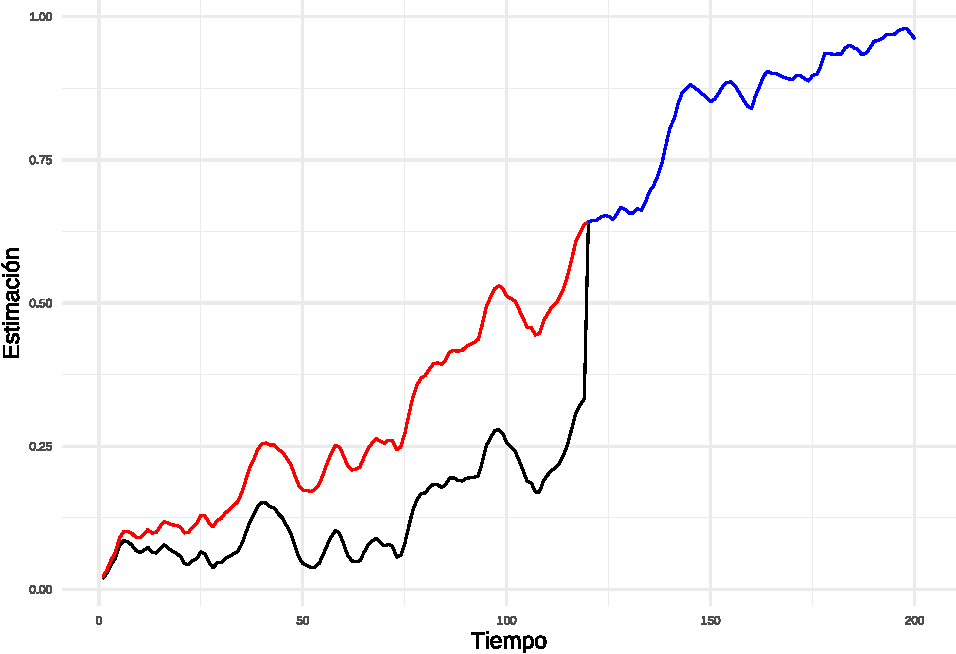
\includegraphics{20Empalme_files/figure-latex/fig204-1.pdf}
\caption{\label{fig:fig204}Empalme de series de tiempo usando un modelo estructural. La línea negra corresponde a la serie regular; la línea azul representa la serie nueva; la línea roja denota la serie empalmada. Fuente: elaboración propia.}
\end{figure}

Por último, en el caso en el que se disponga de ambas series en paralelo, también es posible proponer un modelo estructural bivariado. Asumiendo que las dos series no tienen componente estacional, podemos formular el modelo estructural bivariado para el vector \((\hat \theta^{R}_t,\hat \theta^{N}_t)'\) está dado por:

\[
\begin{aligned}
\hat \theta^{R}_t &= L_t+e_{1,t} \\
\hat \theta^{N}_t &= L_t+\beta\delta_t+e_{2,t}
\end{aligned}
\]

Para este modelo estructural, la ecuación de transición toma la misma forma que en el modelo univariado, mientras que la ecuación de medición queda como:

\[
\begin{bmatrix}\hat \theta^{R}_t\\\hat \theta^{N}_t\end{bmatrix}=\begin{bmatrix}
1&0&0\\
1&0&\delta_t
\end{bmatrix}\begin{bmatrix}
L_t\\
R_t\\
\beta
\end{bmatrix}+e_t
\]

Al igual que en el modelo estructural univariado, los resultados de la aplicación logran extraer la estructura de la serie y estimar correctamente el impacto de la intervención. La Figura \ref{fig:fig205} muestra el empalme de las series usando este acercamiento.

\begin{figure}
\centering
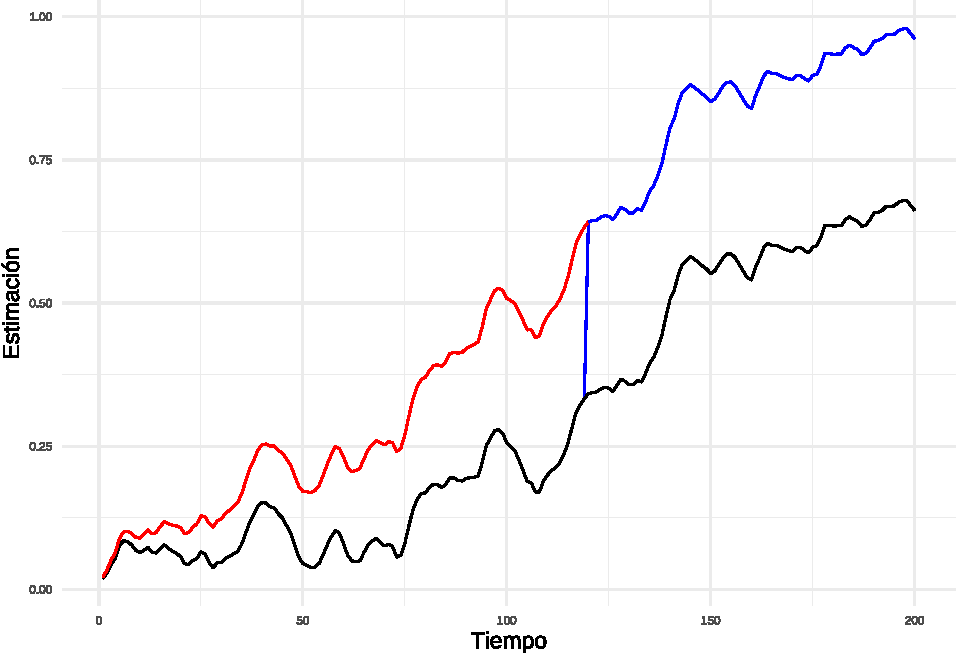
\includegraphics{20Empalme_files/figure-latex/fig205-1.pdf}
\caption{\label{fig:fig205}Empalme de series de tiempo usando un modelo estructural. La línea negra corresponde a la serie regular; la línea azul representa la serie nueva; la línea roja denota la serie empalmada. Fuente: elaboración propia.}
\end{figure}

\hypertarget{appendix-appendix}{%
\appendix}


\hypertarget{una-perspectiva-regional-de-las-encuestas-de-hogares}{%
\chapter{Una perspectiva regional de las encuestas de hogares}\label{una-perspectiva-regional-de-las-encuestas-de-hogares}}

Esta sección presenta una breve descripción del estado de la situación de las encuestas de hogares en la región. Aunque no se pretende hacer un resumen exhaustivo de cada encuesta y de sus componentes metodológicos, el lector podrá enterarse de las características principales de la encuestas de hogares y sus condiciones de aplicación.

Algunas de estas encuestas son estandarizadas por la División de Estadísticas de la CEPAL en su banco de datos de encuestas de hogares, llamado BADEHOG, con el cual se generan estimaciones comparables de indicadores de pobreza y desigualdad año tras año para América Latina \citep{BADEHOG}. Esta iniciativa tuvo su desarrollo principal en la década de los años 90 del siglo pasado, con el fin de recopilar anualmente las encuestas de hogares de 18 países de América Latina. Estas encuestas de hogares tienen la particularidad de que miden el ingreso y se utilizan para estimar pobreza y desigualdad distributiva. Actualmente BADEHOG tiene en su haber encuestas desde 1980 en adelante. BADEHOG constituye un insumo esencial para la creación de indicadores sociales armonizados en América Latina.

\hypertarget{descripciuxf3n-de-algunas-encuestas-por-pauxedses}{%
\section{Descripción de algunas encuestas por países}\label{descripciuxf3n-de-algunas-encuestas-por-pauxedses}}

\hypertarget{argentina}{%
\subsection{Argentina}\label{argentina}}

El Instituto Nacional de Estadística y Censo lleva a cabo de forma trimestral la \emph{Encuesta Permanente de Hogares} la cual permite caracterizar la situación social de los individuos y las familias teniendo en cuenta su inserción en la estructura social y económica \citep{INDEC-AR}. Esta encuesta revela información sobre características demográficas básicas de los miembros del hogar y su situación laboral, ingresos de los individuos, así como sus características educacionales y de migración. También permite caracterizar las viviendas.

Por otro lado, la \emph{Encuesta Nacional de Gastos de los Hogares} proporciona información sobre los hogares argentinos mediante el relevamiento de sus gastos e ingresos. Sus resultados contribuyen con la elaboración de la canasta de bienes y servicios que se utiliza para medir el índice de precios al consumidor, así como aportan información para la estimación de la pobreza y la producción de indicadores de la economía nacional \citep{INDEC-AR2}.

\hypertarget{bolivia}{%
\subsection{Bolivia}\label{bolivia}}

El objetivo principal de la \emph{Encuesta Continua de Empleo} aplicada anualmente por el Instituto Nacional de Estadística es suministrar información sobre las condiciones de vida de los hogares, a partir de la recopilación de información de variables económicas y demográficas de la población para le diseño de programas sociales y formulación, evaluación y seguimiento de las políticas públicas. Dentro de los ejes temáticos que aborda la encuesta se encuentran la estimación de las necesidades básicas insatisfechas, el acceso a los servicios públicos, la caracterización demográfica de los individuos, los desplazamientos de la población en los últimos cinco años, el estado de salud de los miembros del hogar, las características educativas, las condiciones de ocupación, los ingresos percibidos y los gastos del hogar. Esta encuesta permite medir oportunamente los indicadores de pobreza de la población boliviana, así como el acceso a la vivienda, los servicios básicos, la educación, entre otros. Mediante la EH, el INE obtiene estadísticas e indicadores socioeconómicos y demográficos de la población que son necesarias para la formulación, evaluación, monitoreo y seguimiento de las políticas del estado \citep{INE-BO}.

\hypertarget{brasil}{%
\subsection{Brasil}\label{brasil}}

La \emph{Pesquisa Nacional por Amostra de Domicílios} es implementada anualmente por el Instituto Brasileiro de Geografia e Estatística. Esta encuesta tiene como objetivo producir información básica para el estudio de la evolución económica de Brasil y la publicación continua de indicadores demográficos. Los constructos de ingreso, gastos y empleo son evaluados de forma continua, mientras que anualmente se abordan otros módulos de interés. Otros temas adicionales investigados en la encuesta están relacionados con las características de la vivienda, migración de los individuos del hogar, trabajo infantil, fecundidad, salud y seguridad alimentaria, uso de las tecnologías de información, transferencias de renta, uso del tiempo, entre otros \citep{IBGEBR_2017}.

La \emph{Pesquisa de Orçamentos Familiares} tiene como propósito obtener informaciones generales sobre domicilios, familias y personas, hábitos de consumo, gastos y recibos de las familias encuestadas, teniendo como unidad de recolección los domicilios. Permite actualizar la canasta básica de consumo y obtiene nuevas estructuras de ponderación para los índices de precios que componen el Sistema Nacional de Índices de Precios al Consumidor del IBGE y otras instituciones \citep{IBGE-BR2018}

\hypertarget{chile}{%
\subsection{Chile}\label{chile}}

El Ministerio de Desarrollo Social y Familia aplica la \emph{Encuesta de Caracterización Socioeconómica Nacional} de forma bianual y su objetivo es conocer periódicamente la situación de los hogares y de la población, especialmente de aquella en situación de pobreza, con relación a aspectos demográficos, de educación, salud, vivienda, trabajo e ingresos. De esta forma, la encuesta permite estimar la magnitud de la pobreza y la distribución del ingreso; identificar carencias y demandas de la población en las áreas señaladas; y evaluar las distintas brechas que separan a los diferentes segmentos sociales y ámbitos territoriales. Esta encuesta también permite medir la eficacia de los programas sociales que ha implementado el gobierno para la toma de decisiones de política pública. Entre otros, la encuesta se compone de los módulos de registro, que incluye información de identificación de los hogares; educación, que indaga por la situación educacional de los miembros del hogar y la cobertura del sistema educativo; trabajo, que permite conocer la evolución de la situación laboral y ocupacional para formular y evaluar políticas públicas; ingresos, que permite investigar las condiciones de vida de los miembros del hogar; salud, en donde se indaga por la cobertura de los programas públicos \citep{MDS-CL_2015}.

La \emph{Encuesta de Presupuestos Familiares} es una encuesta socioeconómica aplicada a hogares, cuyo propósito es recopilar información sobre gastos en los que estos incurren y los ingresos que perciben en un período de tiempo determinado. La información que recoge la EPF es la base para elaborar la canasta de bienes y servicios con la cual se calcula el Índice de Precios al Consumidor y también se utiliza para actualizar las líneas de pobreza extrema y pobreza empleadas en las estadísticas oficiales de Chile \citep{INE_CL}.

\hypertarget{colombia}{%
\subsection{Colombia}\label{colombia}}

El Departamento Nacional de Estadística aplica la \emph{Gran Encuesta Integrada de Hogares} de forma mensual. Esta encuesta tiene como objetivo general proporcionar información económica básica con énfasis en las características de la fuerza de trabajo. Además indaga por constructos sociales y económicos. Dentro de la temática social, se pregunta por el acceso a la educación formal, condiciones de calidad de vida, ingresos y gastos, trabajo infantil y aspectos de seguridad y convivencia ciudadana. La temática económica indaga aspectos relacionados con industria, comercio, servicios y transporte. El instrumento de recolección de la encuesta está dividido en capítulos que abordan la información relacionada con la vivienda y el hogar, además de hacer un registro de las personas que conforman el hogar y su relación con el jefe de hogar, estableciendo así una caracterización general de la población. Por lo demás también indaga por el acceso a la seguridad social en salud, las características educativas de las población mayor de tres años y clasifica a las personas mayores de 10 años en las categorías establecidas para la fuerza de trabajo \citep{DANE-COL_2017}.

La \emph{Encuesta Nacional de Presupuestos de los Hogares} es una investigación dirigida a los hogares, en la cual se indagan en forma detallada todos los ingresos de los miembros del hogar de 10 años y más (ingresos por trabajo, ingresos de capital, subsidios, transferencias, ingresos ocasionales, etc) así como todos los posibles gastos en que puede incurrir un hogar, captados con diferentes periodicidades (semanal, mensual, trimestral y anual). Dentro de sus objetivos específicos está el obtener información para realizar actualizaciones del IPC, estimar líneas de indigencia y pobreza, caracterizar la distribución del ingreso del hogar con características demográficas, educativas y económicas, etc. \citep{DANE-COL_2018}

\hypertarget{costa-rica}{%
\subsection{Costa Rica}\label{costa-rica}}

La \emph{Encuesta Nacional de Hogares}, llevada a cabo por el Instituto Nacional de Estadística y Censos de forma anual, tiene como objetivo producir estimaciones del nivel de bienestar de la población, especialmente centrados en la conformación del ingreso de los hogares, su distribución y características de los hogares y la población en situación de pobreza. El constructo principal y la motivación de esta encuesta está referido a la pobreza multidimensional y la desigualdad midiendo el ingreso promedio de los hogares por fuente y su distribución, su incidencia y severidad, así como las brechas y perfiles. Esta encuesta permite obtener estas estimaciones a nivel de región y ha incluido algunos módulos especiales de victimización, gasto en los hogares y acceso a la salud \citep{INEC-CR_2017}.

La \emph{Encuesta Nacional de Ingresos y Gastos} de los Hogares proporciona datos económicos de los hogares para conocer las diversas fuentes de ingresos que tienen éstos y cómo distribuyen sus ingresos en la adquisición de los diferentes bienes y servicios. La encuesta suministra gran parte de la información necesaria para estimar la secuencia de cuentas del Sector Hogares, dentro del sistema de Cuentas Nacionales del país. También brinda los datos necesarios para actualizar la canasta de bienes y servicios que componen el Índice de Precios al Consumidor (IPC); entre otros estudios sobre la estructura de gastos de los hogares y la distribución del ingreso \citep{INEC-CR_2018}.

\hypertarget{cuba}{%
\subsection{Cuba}\label{cuba}}

La Oficina Nacional de Estadística e Información aplica anualmente la \emph{Encuesta Nacional de Ocupación} y la \emph{Encuesta de Situación Económica de los Hogares}. Lo objetivos de estas investigaciones se centran en la caracterización de la población en edad de trabajar y su ocupación, así como en obtener indicadores para la toma de decisiones en materia de políticas sociales y económicas \citep{ONE-CU}.

Estas encuestas investigan temas relacionados como las características de las viviendas, la educación en los hogares, las características económicas de los miembros del hogar (para las personas mayores de 15 años), la movilidad laboral y los ingresos en el hogar.

\hypertarget{ecuador}{%
\subsection{Ecuador}\label{ecuador}}

El Instituto Nacional de Estadística y Censos cuenta con el Sistema Integrado de Encuestas a Hogares con el cual se produce información de las características demográficas y económicas de los hogares y personas. Entre otras, el sistema cuenta con la \emph{Encuesta de Empleo, Desempleo y Subempleo en Área Urbana y Rural}, con periodicidad mensual; la \emph{Encuesta Nacional de Ingresos y Gastos de los Hogares Urbanos y Rurales}, con periodicidad quinquenal; y la \emph{Encuesta de Condiciones de Vida}, con periodicidad cuatrienal. Las anteriores encuestas cuentan con temas en común, como condiciones de vivienda, caracterización de los hogares, educación de los miembros del hogar, condición de la actividad económica de los individuos, acceso a servicios públicos e ingreso \citep{INEC-EC}.

Por ejemplo, la \emph{Encuesta de Condiciones de Vida} permite obtener indicadores sobre los niveles de vida y el bienestar de la población relacionando varios factores como educación, salud, pobreza e inequidad para la aplicación de política pública. La ECV 2013 -- 2014 incluye temas nuevos como hábitos, prácticas y uso del tiempo de los hogares, bienestar psicosocial, percepción del nivel de vida, capital social, seguridad ciudadana y retorno migratorio \citep{INEC2-EC}.

\hypertarget{el-salvador}{%
\subsection{El Salvador}\label{el-salvador}}

La \emph{Encuesta de Hogares de Propósitos Múltiples} es implementada anualmente por la Dirección General de Estadística y Censos y su objetivo es generar información estadística relacionada con las condiciones económicas y demográficas de la población con el fin de evaluar y focalizar las políticas públicas del gobierno para elevar el bienestar de la población. Esta encuesta indaga por la información general de los miembros del hogar, su situación educacional (analfabetismo, escolaridad y asistencia), también pregunta por las características de la vivienda y la situación de ocupación de la población Contiene a su vez un módulo de actividad del productor agropecuario que recolecta información acerca de la tenencia de la tierra, superficie cultivada, y la actividad agropecuaria del entrevistado. Por último también pregunta acerca de variables de salud, dinámica de las remesas y los gastos del hogar \citep{DIGESTYC-SV}.

La \emph{Encuesta de Ingresos y Gastos de los Hogares} permite determinar la canasta de mercado para el desarrollo del Índice de Precios al Consumidor (IPC), el consumo privado en las Cuentas Nacionales (CN) y para análisis de bienestar y pobreza. La encuesta también mide la educación, el empleo, las condiciones de la vivienda, la posesión de bienes durables, la construcción y los otros negocios y actividades agrícolas relacionados al hogar \citep{DIGESTYC2-SV}.

\hypertarget{guatemala}{%
\subsection{Guatemala}\label{guatemala}}

El Instituto Nacional de Estadística aplica de manera semestral la \emph{Encuesta Nacional de Empleo e Ingresos}. Los objetivos de esta encuesta son dar seguimiento a un conjunto básico de variables e indicadores del mercado laboral y producir información que permita conocer el comportamiento y evolución del empleo, el desempleo, las características, composición, estructura y funcionamiento del mercado de trabajo. Además de investigar aspectos generales del mercado laboral, esta encuesta indaga las características de informalidad, ocupación y formas de contratación. Tiene un componente de ingresos, así como algunos aspectos demográficos y de educación en los hogares de Guatemala. Algunos cambios recientes han incluido módulos de uso del tiempo y uso de las tecnologías de información \citep{INE-GT}.

La \emph{Encuesta Nacional de Condiciones de Vida} tiene como principal objetivo, conocer y evaluar las condiciones de vida de la población, así como determinar los niveles de pobreza existentes en Guatemala y los factores que los determinan caracterizando a la población pobre t no pobre del país, brindando resultados a nivel nacional, regional y departamental \citep{INE2-GT}.

\hypertarget{honduras}{%
\subsection{Honduras}\label{honduras}}

La \emph{Encuesta Permanente de Hogares de Propósitos Múltiples} es una investigación semestral dirigida por el Instituto Nacional de Estadística de Honduras con el fin de recolectar información sobre las características generales de la población hondureña, en términos de vivienda, tasas de ocupación, desocupación y subempleo, ingreso en los hogares y acceso a las tecnologías de la información \citep{INE-HN}.

La \emph{Encuesta de Condiciones de Vida de los Hogares} es una investigacion de carácter multipropósito que permite conocer los diferentes aspectos y dimensiones del bienestar de los hogares. Incluye, además de los ingresos y gastos de las unidades familiares, un conjunto de variables que describen los niveles de vida de los hogares. En este sentido esta publicación incorpora información sobre: Características de la vivienda, demografía, migración, educación, salud, antropometría, mercado laboral (género, personas con problemas laborales, trabajo infantil y juvenil), ingresos y gasto de los hogares, pobreza y otros temas de importancia \citep{INE2-HN}.

\hypertarget{muxe9xico}{%
\subsection{México}\label{muxe9xico}}

La \emph{Encuesta Nacional de Ocupación y Empleo} aplicada cada dos años por el Instituto Nacional de Estadística y Geografía tiene como objetivo proporcionar un panorama estadístico del comportamiento de los ingresos y gastos de los hogares en cuanto a su monto, procedencia y distribución; adicionalmente, ofrece información sobre las características ocupacionales y demográficas de los integrantes del hogar, así como las características de la infraestructura de la vivienda y el equipamiento del hogar. Además de lo anterior, la encuesta cubre algunos constructos como percepciones y erogaciones financieras y de capital de los hogares y sus integrantes, características de la vivienda, características demográficas de los residentes de la vivienda, condición de actividad y características ocupacionales de los integrantes del hogar de 12 y más años, equipamiento del hogar y acceso a servicios \citep{INEGI-MX}.

La \emph{Encuesta Nacional de Ingresos y Gastos de los Hogares} tiene como objetivo proporcionar un panorama estadístico del comportamiento de los ingresos y gastos de los hogares en cuanto a su monto, procedencia y distribución; adicionalmente, ofrece información sobre las características ocupacionales y sociodemográficas de los integrantes del hogar, así como las características de la infraestructura de la vivienda y el equipamiento del hogar \citep{INEGI2-MX}.

\hypertarget{nicaragua}{%
\subsection{Nicaragua}\label{nicaragua}}

Nicaragua lleva a cabo de forma trimestral la \emph{Encuesta Nacional de Hogares Sobre la Medición de Niveles de Vida}, a través del Instituto Nacional de Información de Desarrollo, cuyo objetivo general es producir información continua sobre características ocupacionales, demográficas y evolución de la pobreza. Esta encuesta indaga exhaustivamente acerca de las características demográficas de todos los miembros del hogar, además de la actividad económica y condición de los individuos en edad de trabajar y sus ingresos. Indaga también por el estado de la vivienda y sus características. Esta encuesta también dispone de las variables necesarias para la construcción de otras medidas de bienestar, como agregado de ingreso, necesidades básicas insatisfechas, etc. \citep{INIDE-NI}.

\hypertarget{panamuxe1}{%
\subsection{Panamá}\label{panamuxe1}}

El Instituto Nacional de Estadística y Censo de Panamá aplica anualmente la \emph{Encuesta de Propósitos Múltiples} cuyos objetivos están encaminados a la producción de estadísticas de empleo e ingresos y a la estimación de la situación del mercado Laboral. Como la principal finalidad de la encuesta es la medición de los cambios del mercado laboral, se indaga por la condición de actividad económica, ocupación, lugar de trabajo e ingresos. También se debe resaltar que la encuesta aborda, de manera no continua, algunos temas relacionados con el acceso a la tecnología, el interés y colaboración con actividades de protección y conservación de los recursos naturales, dinámica de turismo en los hogares, identificación de recibo o envío de remesas y migración (desplazamiento interno y externo de la población durante un intervalo), así como el uso de servicios financieros \citep{INEC-PA}.

La \emph{Encuesta de Ingresos y Gastos de los Hogares} se realiza para actualizar la información de los ingresos de los hogares en panamá y como estos distribuyen los presupuestos para obtener diferentes bienes y servicios. La información recopilada tiene como principales objetivos obtener coeficientes de ponderación y canastas de consumo que serán utilizadas para el cálculo del IPC y la CBFA. Por otra parte permite estructurar la demanda de los hogares en bienes de consumo privado \citep{INEC2-PA}.

\hypertarget{paraguay}{%
\subsection{Paraguay}\label{paraguay}}

La \emph{Encuesta Permanente de Hogares} ejecutada anualmente por la Dirección General de Estadística, Encuestas y Censos tiene como objetivo la generación de indicadores anuales sobre las principales características de las condiciones de vida de la población y sus resultados son utilizados para las estimaciones de pobreza. Algunos de los constructos que investiga esta encuesta se relacionan con las características de las viviendas, educación de los miembros del hogar, salud, empleo e ingresos, condición de ocupación, acceso a programas sociales del gobierno y remesas \citep{DGEEC-PY}.

La \emph{Encuesta de Ingresos y Gastos y de Condiciones de Vida} tiene como principal objetivo actualizar la estructura de la Canasta Básica de Alimentos y la Canasta Total Familiar, cuyos valores constituyen las líneas de pobreza, así como el de caracterizar y analizar las Condiciones de Vida de la Población del Paraguay. Esta información es recopilada a través de cuestionarios que recogen datos acerca de temas de educación, salud, ingresos, actividades independientes no agropecuarias, perfiles de ingresos y de tipo productivo, etc. \citep{DGEEC2-PY}.

\hypertarget{peruxfa}{%
\subsection{Perú}\label{peruxfa}}

La \emph{Encuesta Nacional de Hogares sobre Condiciones de Vida y Pobreza} es una investigación mensual que realiza el Instituto Nacional de Estadística e Informática cuyo objetivo es la obtención de información estadística, social, demográfica y económica, proveniente de los hogares para el cálculo de indicadores para la medición de aspectos económicos y sociales; y conocer y explicar los determinantes o factores causales del comportamiento de dichos aspectos para el diseño, monitoreo y medición de resultados de las políticas públicas. Dentro de los módulos que la encuesta aborda se encuentran la caracterización de la vivienda y el hogar, la educación de los miembros del hogar, así como su estado de salud, la condición de actividad de empleo, ingresos y gastos, acceso a programas sociales, participación ciudadana, así como la percepción de la gobernabilidad y algunos tópicos concernientes al fenómeno de la discriminación \citep{INEI-PE_2016}.

\hypertarget{repuxfablica-dominicana}{%
\subsection{República Dominicana}\label{repuxfablica-dominicana}}

La Oficina Nacional de Estadística cuenta con un Sistema Integrado de Encuestas de Hogares que agrupa, entre otras, a la \emph{Encuesta Nacional de Hogares de Propósitos Múltiples}, con periodicidad anual y la \emph{Encuesta Nacional de Fuerza de Trabajo}, con periodicidad semestral. La primera es una encuesta orientada a recopilar periódicamente datos sobre diferentes temas sociales, económicos y ambientales; mientras que la segunda está orientada a obtener indicadores de la población en edad de trabajar y su ocupación. Algunos de los aspectos principales que evalúa el sistema de encuestas de hogares están relacionados con las condiciones y características de las viviendas y personas, así como con la educación de los miembros del hogar, el acceso a tecnologías de información y algunas características de seguridad ciudadana y convivencia \citep{ONE-DO}.

Por ejemplo, la Encuesta Nacional de Ingresos y Gastos de los Hogares es un estudio estadístico que se realiza generalmente cada 10 años para conocer la distribución del gasto en bienes y servicios de consumo de los hogares, así como los ingresos que éstos obtienen por diferentes fuentes para financiar su consumo. Dentro de sus objetivos se encuentra el obtener información para conocer el nivel y la estructura de los gastos de consumo de los hogares y su distribución en rubros de: alimentos y bebidas no alcohólicas; bebidas alcohólicas, tabaco y estupefacientes; prendas de vestir y calzado; alojamiento, agua, electricidad, gas, y otros combustibles; muebles, artículos para el hogar y para la conservación ordinaria del hogar; salud; transporte; comunicaciones; recreación y cultura; educación; restaurantes y hoteles y, bienes y servicios diversos \citep{ONE2-DO}.

\hypertarget{uruguay}{%
\subsection{Uruguay}\label{uruguay}}

El Instituto Nacional de Estadística aplica mensualmente la \emph{Encuesta Continua de Hogares} que brinda los indicadores oficiales del mercado laboral (actividad, empleo y desempleo) y de ingresos de los hogares y las personas. Además esta encuesta permite estimar la proporción de hogares y personas por debajo de la línea de pobreza y de indigencia de forma anual. El cuestionario de la encuesta indaga por las características de las viviendas y de los hogares, así como las características demográficas de los miembros del hogar y algunas variables de migración, acceso a la salud, educación, alimentación y uso de las tecnologías de información. De la misma forma, la encuesta aborda de manera exhaustiva los constructos de actividad laboral, ingresos y egresos personales y del hogar \citep{INE-UY_2016}.

La \emph{Encuesta de Gastos e Ingresos de los Hogares}, se realiza aproximadamente cada 10 años y permite conocer la realidad económica y social del país. A partir de los resultados obtenidos, se podrá elaborar una canasta actualizada para el Índice de Precios al Consumo (IPC) y también determinar las líneas de indigencia y de pobreza nacionales. Esta es una encuesta muy importante, ya que a partir de los datos brindados, se puede obtener la información de base para elaborar indicadores que interesan a toda la sociedad, como son los de inflación y pobreza \citep{INE2-UY}.

\hypertarget{venezuela}{%
\subsection{Venezuela}\label{venezuela}}

La \emph{Encuesta de Hogares por Muestreo} es una investigación que desarrolla el Instituto Nacional de Estadística con periodicidad semestral. Esta encuesta de propósitos múltiples brinda información sobre la estructura y evolución del mercado de trabajo, así como de las características económicas y demográficas de la población. Algunos de las temáticas más relevantes de esta encuesta se centran en la actividad económica de los miembros del hogar y su estado de empleo, así como la caracterización de las viviendas y de los hogares y algunas variables educativas, que dan origen a indicadores de analfabetismo. Asimismo, la \emph{Encuesta Nacional de Presupuestos Familiares}, es una investigación por muestreo dirigida a los hogares, que tiene por objeto obtener información sobre sus ingresos, egresos, características de las viviendas que habitan, composición de los hogares y otras variables económicas y sociales de sus miembros. Dentro de sus objetivos se encuentra conocer los cambios ocurridos en los patrones de consumo de los hogares, actualizar la canasta de bienes y servicios y las ponderaciones del IPC, etc. \citep{INE-VE}.

\newpage
\blandscape

\begin{longtable}[]{@{}
  >{\raggedright\arraybackslash}p{(\columnwidth - 10\tabcolsep) * \real{0.1507}}
  >{\raggedright\arraybackslash}p{(\columnwidth - 10\tabcolsep) * \real{0.4589}}
  >{\raggedright\arraybackslash}p{(\columnwidth - 10\tabcolsep) * \real{0.0685}}
  >{\raggedright\arraybackslash}p{(\columnwidth - 10\tabcolsep) * \real{0.0959}}
  >{\raggedright\arraybackslash}p{(\columnwidth - 10\tabcolsep) * \real{0.0685}}
  >{\raggedright\arraybackslash}p{(\columnwidth - 10\tabcolsep) * \real{0.1575}}@{}}
\caption{\emph{Características de las algunas encuestas repetidas en América Latina.}}\tabularnewline
\toprule()
\begin{minipage}[b]{\linewidth}\raggedright
País
\end{minipage} & \begin{minipage}[b]{\linewidth}\raggedright
Nombre de la encuesta
\end{minipage} & \begin{minipage}[b]{\linewidth}\raggedright
Tipo
\end{minipage} & \begin{minipage}[b]{\linewidth}\raggedright
Periodicidad
\end{minipage} & \begin{minipage}[b]{\linewidth}\raggedright
Rotación
\end{minipage} & \begin{minipage}[b]{\linewidth}\raggedright
Muestra de viviendas
\end{minipage} \\
\midrule()
\endfirsthead
\toprule()
\begin{minipage}[b]{\linewidth}\raggedright
País
\end{minipage} & \begin{minipage}[b]{\linewidth}\raggedright
Nombre de la encuesta
\end{minipage} & \begin{minipage}[b]{\linewidth}\raggedright
Tipo
\end{minipage} & \begin{minipage}[b]{\linewidth}\raggedright
Periodicidad
\end{minipage} & \begin{minipage}[b]{\linewidth}\raggedright
Rotación
\end{minipage} & \begin{minipage}[b]{\linewidth}\raggedright
Muestra de viviendas
\end{minipage} \\
\midrule()
\endhead
Argentina & Encuesta Permanente de Hogares & Panel & Trimestral & 50\% & 25000 \\
Bolivia & Encuesta Continua de Hogares & Panel & Mensual & 25\% & 10000 \\
Brasil & Pesquisa Nacional por Amostra de Domicilios & Repetida & Anual & - & 115000 \\
Brasil & Pesquisa Nacional por Amostra de Domicilios Continua & Panel & Mensual & 20\% & 70000 \\
Chile & Encuesta de Caracterización Socioeconómica Nacional & Repetida & Bienal & - & 84000 \\
Colombia & Gran Encuesta Integrada de Hogares & Repetida & Mensual & - & 20000 \\
Costa Rica & Encuesta Nacional de Hogares & Repetida & Anual & - & 13000 \\
Cuba & Encuesta Nacional de Ocupación & Panel & Anual & 33\% & 63000 \\
Ecuador & Encuesta de Empleo, Desempleo y Subempleo en Área Urbana y Rural & Panel & Trimestral & 50\% & 16000 \\
El Salvador & Encuesta de Hogares de Propósitos Múltiples & Repetida & Anual & - & 20000 \\
Guatemala & Encuesta Nacional de Empleo e Ingresos & Repetida & Semestral & - & 6000 \\
Honduras & Encuesta Permanente de Hogares de Propósitos Múltiples & Repetida & Semestral & - & 7200 \\
México & Encuesta Nacional de Ingresos y Gastos de los Hogares & Repetida & Bienal & - & 20000 \\
Nicaragua & Encuesta Nacional de Hogares Sobre la Medición de Niveles de Vida & Panel & Trimestral & 20\% & 7500 \\
Panamá & Encuesta de Propósitos Múltiples & Repetida & Anual & - & 15000 \\
Paraguay & Encuesta Permanente de Hogares & Repetida & Anual & 50\% & 6000 \\
Perú & Encuesta Nacional de Hogares sobre Condiciones de Vida y Pobreza & Panel & Anual & 20\% & 32000 \\
República Dominicana & Encuesta Nacional de Hogares de Propósitos Múltiples & Repetida & Anual & - & 34000 \\
República Dominicana & Encuesta Nacional de Fuerza de Trabajo & Panel & Semestral & 25\% & 10000 \\
Uruguay & Encuesta Continua de Hogares & Repetida & Mensual & - & 53000 \\
Venezuela & Encuesta de Hogares por Muestreo & Repetida & Semestral & - & 45000 \\
\bottomrule()
\end{longtable}

\newpage

\begin{longtable}[]{@{}
  >{\raggedright\arraybackslash}p{(\columnwidth - 6\tabcolsep) * \real{0.1864}}
  >{\raggedright\arraybackslash}p{(\columnwidth - 6\tabcolsep) * \real{0.5593}}
  >{\raggedright\arraybackslash}p{(\columnwidth - 6\tabcolsep) * \real{0.0932}}
  >{\raggedright\arraybackslash}p{(\columnwidth - 6\tabcolsep) * \real{0.1610}}@{}}
\caption{\emph{Características de las algunas encuestas transversales en América Latina.}}\tabularnewline
\toprule()
\begin{minipage}[b]{\linewidth}\raggedright
País
\end{minipage} & \begin{minipage}[b]{\linewidth}\raggedright
Nombre
\end{minipage} & \begin{minipage}[b]{\linewidth}\raggedright
Año
\end{minipage} & \begin{minipage}[b]{\linewidth}\raggedright
Tamaño de Muestra
\end{minipage} \\
\midrule()
\endfirsthead
\toprule()
\begin{minipage}[b]{\linewidth}\raggedright
País
\end{minipage} & \begin{minipage}[b]{\linewidth}\raggedright
Nombre
\end{minipage} & \begin{minipage}[b]{\linewidth}\raggedright
Año
\end{minipage} & \begin{minipage}[b]{\linewidth}\raggedright
Tamaño de Muestra
\end{minipage} \\
\midrule()
\endhead
Argentina & Encuesta Nacional de Gastos de los Hogares & 2017-2018 & 45000 \\
Bolivia & Encuesta de Hogares & 2017 & 11136 \\
Brasil & Encuesta de Presupuestos familiares & 2008-2009 & 53154 \\
Chile & VIII Encuesta de Presupuestos Familiares & 2016-2017 & 15239 \\
Colombia & Encuesta Nacional de Presupuestos de los Hogares & 2016-2017 & 87201 \\
Costa Rica & Encuesta Nacional de Ingresos y Gastos de los hogares & 2018-2019 & 9828 \\
Ecuador & Encuesta de Condiciones de Vida & 2013-2014 & 29052 \\
El Salvador & Encuesta de Ingresos y Gastos de Hogares & 2005-2006 & 4576 \\
Guatemala & Encuesta Nacional de Condiciones de Vida & 2014 & 11536 \\
Honduras & Encuesta de Condiciones de Vida de los Hogares & 2004 & 8155 \\
México & Encuesta Nacional de Ingresos y Gastos de los Hogares & 2016 & 81515 \\
Nicaragua & Encuesta Nacional de Hogares sobre Medición de Nivel de Vida & 2014 & 6851 \\
Panamá & Encuesta de Ingresos y Gastos de los Hogares & 2007-2008 & 10152 \\
Paraguay & Encuesta de Ingresos y Gastos de Condiciones de Vida & 2011-2012 & 6000 \\
Perú & Encuesta Nacional de Hogares sobre Condiciones de Vida y Pobreza & 2017 & 36996 \\
República Dominicana & Encuesta Nacional de Ingresos y Gastos de los hogares & 2006-2007 & 8358 \\
Uruguay & Encuesta Nacional de Gastos e Ingresos de los Hogares & 2016-2017 & 7500 \\
Venezuela & IV Encuesta Nacional de Presupuestos Familiares & 2008-2009 & 45768 \\
\bottomrule()
\end{longtable}

\elandscape

\hypertarget{software}{%
\chapter{Software}\label{software}}

El diseño y análisis de la información proveniente de las encuestas de hogares debe contemplar el uso exhaustivo de las herramientas computacionales existentes. Esta sección revisa con detalle las aproximaciones computacionales del software estadístico utilizado para realizar cada uno de los procesos estadísticos que se necesitan para lograr el cometido de la publicación de cifras oficiales con altos niveles de precisión y confiabilidad. En particular, para los siguientes procesos:

\begin{enumerate}
\def\labelenumi{\arabic{enumi}.}
\tightlist
\item
  Selección de muestras acorde al diseño de muestreo definido
\item
  Generación de pesos de muestreo para cada individuo y hogar.
\item
  Modelación de la ausencia de respuesta e imputación estadística.
\item
  Calibración de los pesos de muestreo y ajustes por ausencia de respuesta.
\item
  Estimación de los errores de muestreo para cada indicador de interés en los cuadros de producción estadística.
\item
  Análisis de las relaciones multivariantes entre las variables de la encuesta.
\item
  Modelación de las estimaciones para la predicción del parámetro de interés en dominios pequeños.
\end{enumerate}

\citet[sección 7.8]{United_Nations_2005} muestra la importancia de incluir la estructura del diseño de muestreo complejo en la inferencia que se realiza para la estimación de estadísticas oficiales a partir de encuestas de hogares y advierten con un ejemplo empírico que de no hacerlo, es posible que las estimaciones resultantes sean sesgadas y además sus errores de muestreo se vean subestimados. A continuación se muestran algunos de las características más importantes que los paquetes estadísticos computacionales incorporan en el manejo de datos que provienen de estructuras de muestreo complejas como las encontradas en las encuestas de hogares. Una revisión más exhaustiva y detallada que adjunta sintaxis y código computacional puede encontrarse en \citet[Apéndice A]{Heeringa_West_Berglund_2010}.

En general, estas herramientas computacionales están pensadas para hacer más eficiente el uso de las aproximaciones de varianza en muestras complejas, así como las técnicas de replicación para obtener los estimativos de varianza inducidos por el diseño de muestreo \citep{Westat_2007}. Algunos de estos softwares son de uso libre, aunque la mayoría corresponde a productos licenciados cuya licencia debe ser pagada. En general estos productos, además de proveer estadísticas descriptivas (como medias, totales, proporciones, percentiles y razones), permiten ajustar modelos de regresión lineales y logísticos. Todas las estadísticas resultantes están basadas en el diseño de muestreo de la encuesta.

\hypertarget{r}{%
\section{R}\label{r}}

R es un software de uso libre cuyo uso es cada vez más frecuente en la investigación social, puesto que es muy probable encontrar los más recientes hallazgos científicos programados en este software \citep{R_2019}. Al ser de uso libre, los investigadores pueden subir sus propias colecciones de funciones computacionales al repositorio oficial (\texttt{CRAN}) y ponerlas a disposición de la comunidad. El paquete \texttt{samplesize4surveys} \citep{ss4s} permite determinar el tamaño de muestra de individuos y hogares en encuestas de hogares repetidas, tipo panel y con rotación. Los paquetes \texttt{sampling} \citep{Yves} y \texttt{TeachingSampling} \citep{TS} permiten seleccionar muestras probabilísticas desde los marcos de muestreo bajo un gran variedad de diseños y algoritmos de muestreo. El paquete \texttt{survey} \citep{TL}, una vez que el diseño de muestreo ha sido predefinido mediante la función \texttt{svydesign()}, permite analizar datos provenientes de encuestas de hogares y obtener estimaciones apropiadas de los errores estándar.

\hypertarget{stata}{%
\section{STATA}\label{stata}}

El entorno \texttt{svy} provee un conjunto de herramientas para hacer una inferencia apropiada de las estadísticas oficiales provenientes de encuestas de hogares \citep{STATA_2017}. El comando \texttt{svyset} permite especificar las variables que identifican las características del diseño de muestreo de la encuesta, como los pesos de muestreo, los conglomerados y los estratos. El comando \texttt{svydescribe} proporciona tablas que describen los estratos y las unidades de muestra para una determinada etapa de la encuesta. Una vez cargadas las definiciones del diseño de muestreo, cualquier modelo puede ser estimado y sus estadísticos resultantes estarán basados en el diseño de muestreo de la encuesta. El entorno \texttt{svy} también permite la ejecución de algunos comandos predictivos.

\hypertarget{spss}{%
\section{SPSS}\label{spss}}

El módulo \texttt{complex\ samples} de \texttt{SPSS} \citep{IBM_2017} incorpora la selección de muestras complejas mediante la definición de un esquema de muestreo establecido por el usuario. Luego, es necesario crear un plan de análisis mediante la asignación de variables de diseño, métodos de estimación y tamaños de las unidades de muestreo. Una vez definido el plan de muestreo, el módulo integra la posibilidad de estimar conteos, estadísticas descriptivas y celdas de tablas cruzadas. También es posible realizar estimaciones de razones y de coeficientes de regresión en modelos lineales, junto con las respectivas estadísticas de pruebas de hipótesis. Por último el módulo permite estimar modelos no lineales, como regresiones logísticas, regresiones ordinales o regresiones de Cox.

\hypertarget{sas}{%
\section{SAS}\label{sas}}

Este software estadístico incluye un procedimiento para la selección de muestras probabilísticas llamado \texttt{SURVEYSELECT} que integra los métodos de selección más comunes como muestreo aleatorio simple, muestreo sistemático, muestreo con probabilidad proporcional al tamaño, y algunas herramientas de afijación en los estratos. Para analizar los datos provenientes de muestras complejas se han programado algunos procedimientos \citep{SAS_2017}. \texttt{SURVEYMEANS}, que estima totales, medias, proporciones, y percentiles, junto con sus respectivos errores estándar, límites de los intervalos de confianza y pruebas de hipótesis. \texttt{SURVEYFREQ}, estima las estadísticas descriptivas (como totales y proporciones) de interés en tablas de una y dos vías, brinda las estimaciones del error de muestreo, y realiza un análisis de la bondad del ajuste de las estimaciones, independencia, riesgos y razones de \emph{odds}. \texttt{SURVEYREG} y \texttt{SURVEYLOGISTIC} ajustan modelos de regresión lineal y logísticas, respectivamente. Estos procedimientos estiman los coeficientes de regresión, con sus respectivos errores, y adjunta un análisis exhaustivo de las propiedades de los modelos. Por último, \texttt{SURVEYPHREG} ajusta modelos de riesgos utilizando técnicas de máxima-pseudo verosimilitud.

\hypertarget{referencias}{%
\chapter*{Referencias}\label{referencias}}
\addcontentsline{toc}{chapter}{Referencias}

  \bibliography{CEPAL.bib}

\end{document}
